% Options for packages loaded elsewhere
\PassOptionsToPackage{unicode}{hyperref}
\PassOptionsToPackage{hyphens}{url}
%
\documentclass[
]{book}
\usepackage{amsmath,amssymb}
\usepackage{lmodern}
\usepackage{iftex}
\ifPDFTeX
  \usepackage[T1]{fontenc}
  \usepackage[utf8]{inputenc}
  \usepackage{textcomp} % provide euro and other symbols
\else % if luatex or xetex
  \usepackage{unicode-math}
  \defaultfontfeatures{Scale=MatchLowercase}
  \defaultfontfeatures[\rmfamily]{Ligatures=TeX,Scale=1}
\fi
% Use upquote if available, for straight quotes in verbatim environments
\IfFileExists{upquote.sty}{\usepackage{upquote}}{}
\IfFileExists{microtype.sty}{% use microtype if available
  \usepackage[]{microtype}
  \UseMicrotypeSet[protrusion]{basicmath} % disable protrusion for tt fonts
}{}
\makeatletter
\@ifundefined{KOMAClassName}{% if non-KOMA class
  \IfFileExists{parskip.sty}{%
    \usepackage{parskip}
  }{% else
    \setlength{\parindent}{0pt}
    \setlength{\parskip}{6pt plus 2pt minus 1pt}}
}{% if KOMA class
  \KOMAoptions{parskip=half}}
\makeatother
\usepackage{xcolor}
\usepackage{color}
\usepackage{fancyvrb}
\newcommand{\VerbBar}{|}
\newcommand{\VERB}{\Verb[commandchars=\\\{\}]}
\DefineVerbatimEnvironment{Highlighting}{Verbatim}{commandchars=\\\{\}}
% Add ',fontsize=\small' for more characters per line
\usepackage{framed}
\definecolor{shadecolor}{RGB}{248,248,248}
\newenvironment{Shaded}{\begin{snugshade}}{\end{snugshade}}
\newcommand{\AlertTok}[1]{\textcolor[rgb]{0.94,0.16,0.16}{#1}}
\newcommand{\AnnotationTok}[1]{\textcolor[rgb]{0.56,0.35,0.01}{\textbf{\textit{#1}}}}
\newcommand{\AttributeTok}[1]{\textcolor[rgb]{0.77,0.63,0.00}{#1}}
\newcommand{\BaseNTok}[1]{\textcolor[rgb]{0.00,0.00,0.81}{#1}}
\newcommand{\BuiltInTok}[1]{#1}
\newcommand{\CharTok}[1]{\textcolor[rgb]{0.31,0.60,0.02}{#1}}
\newcommand{\CommentTok}[1]{\textcolor[rgb]{0.56,0.35,0.01}{\textit{#1}}}
\newcommand{\CommentVarTok}[1]{\textcolor[rgb]{0.56,0.35,0.01}{\textbf{\textit{#1}}}}
\newcommand{\ConstantTok}[1]{\textcolor[rgb]{0.00,0.00,0.00}{#1}}
\newcommand{\ControlFlowTok}[1]{\textcolor[rgb]{0.13,0.29,0.53}{\textbf{#1}}}
\newcommand{\DataTypeTok}[1]{\textcolor[rgb]{0.13,0.29,0.53}{#1}}
\newcommand{\DecValTok}[1]{\textcolor[rgb]{0.00,0.00,0.81}{#1}}
\newcommand{\DocumentationTok}[1]{\textcolor[rgb]{0.56,0.35,0.01}{\textbf{\textit{#1}}}}
\newcommand{\ErrorTok}[1]{\textcolor[rgb]{0.64,0.00,0.00}{\textbf{#1}}}
\newcommand{\ExtensionTok}[1]{#1}
\newcommand{\FloatTok}[1]{\textcolor[rgb]{0.00,0.00,0.81}{#1}}
\newcommand{\FunctionTok}[1]{\textcolor[rgb]{0.00,0.00,0.00}{#1}}
\newcommand{\ImportTok}[1]{#1}
\newcommand{\InformationTok}[1]{\textcolor[rgb]{0.56,0.35,0.01}{\textbf{\textit{#1}}}}
\newcommand{\KeywordTok}[1]{\textcolor[rgb]{0.13,0.29,0.53}{\textbf{#1}}}
\newcommand{\NormalTok}[1]{#1}
\newcommand{\OperatorTok}[1]{\textcolor[rgb]{0.81,0.36,0.00}{\textbf{#1}}}
\newcommand{\OtherTok}[1]{\textcolor[rgb]{0.56,0.35,0.01}{#1}}
\newcommand{\PreprocessorTok}[1]{\textcolor[rgb]{0.56,0.35,0.01}{\textit{#1}}}
\newcommand{\RegionMarkerTok}[1]{#1}
\newcommand{\SpecialCharTok}[1]{\textcolor[rgb]{0.00,0.00,0.00}{#1}}
\newcommand{\SpecialStringTok}[1]{\textcolor[rgb]{0.31,0.60,0.02}{#1}}
\newcommand{\StringTok}[1]{\textcolor[rgb]{0.31,0.60,0.02}{#1}}
\newcommand{\VariableTok}[1]{\textcolor[rgb]{0.00,0.00,0.00}{#1}}
\newcommand{\VerbatimStringTok}[1]{\textcolor[rgb]{0.31,0.60,0.02}{#1}}
\newcommand{\WarningTok}[1]{\textcolor[rgb]{0.56,0.35,0.01}{\textbf{\textit{#1}}}}
\usepackage{longtable,booktabs,array}
\usepackage{calc} % for calculating minipage widths
% Correct order of tables after \paragraph or \subparagraph
\usepackage{etoolbox}
\makeatletter
\patchcmd\longtable{\par}{\if@noskipsec\mbox{}\fi\par}{}{}
\makeatother
% Allow footnotes in longtable head/foot
\IfFileExists{footnotehyper.sty}{\usepackage{footnotehyper}}{\usepackage{footnote}}
\makesavenoteenv{longtable}
\usepackage{graphicx}
\makeatletter
\def\maxwidth{\ifdim\Gin@nat@width>\linewidth\linewidth\else\Gin@nat@width\fi}
\def\maxheight{\ifdim\Gin@nat@height>\textheight\textheight\else\Gin@nat@height\fi}
\makeatother
% Scale images if necessary, so that they will not overflow the page
% margins by default, and it is still possible to overwrite the defaults
% using explicit options in \includegraphics[width, height, ...]{}
\setkeys{Gin}{width=\maxwidth,height=\maxheight,keepaspectratio}
% Set default figure placement to htbp
\makeatletter
\def\fps@figure{htbp}
\makeatother
\setlength{\emergencystretch}{3em} % prevent overfull lines
\providecommand{\tightlist}{%
  \setlength{\itemsep}{0pt}\setlength{\parskip}{0pt}}
\setcounter{secnumdepth}{5}
\usepackage{booktabs}
\usepackage{amsthm}
\usepackage[left=2cm,right=2cm,top=2cm,bottom=2cm]{geometry}
\makeatletter
\def\thm@space@setup{%
  \thm@preskip=8pt plus 2pt minus 4pt
  \thm@postskip=\thm@preskip
}
\makeatother
\ifLuaTeX
  \usepackage{selnolig}  % disable illegal ligatures
\fi
\usepackage[]{natbib}
\bibliographystyle{apalike}
\IfFileExists{bookmark.sty}{\usepackage{bookmark}}{\usepackage{hyperref}}
\IfFileExists{xurl.sty}{\usepackage{xurl}}{} % add URL line breaks if available
\urlstyle{same} % disable monospaced font for URLs
\hypersetup{
  pdftitle={User's guide for LTabundR},
  hidelinks,
  pdfcreator={LaTeX via pandoc}}

\title{User's guide for \texttt{LTabundR}}
\author{}
\date{\vspace{-2.5em}}

\begin{document}
\maketitle

{
\setcounter{tocdepth}{1}
\tableofcontents
}
\hypertarget{overview}{%
\chapter*{Overview}\label{overview}}
\addcontentsline{toc}{chapter}{Overview}

The \texttt{R} package \texttt{LTabundR} offers tools that facilitate and standardize design-based line-transect abundance estimation of cetaceans, based on typical workflow used following NOAA Fisheries ship surveys in the central and eastern Pacific (e.g., \href{https://www.google.com/url?q=https://onlinelibrary.wiley.com/doi/10.1111/j.1748-7692.2006.00032.x\&sa=D\&source=docs\&ust=1676392605333708\&usg=AOvVaw07ERYd9m2kJg0LttBFVyil}{Barlow 2006}, \href{https://spo.nmfs.noaa.gov/content/abundance-and-population-density-cetaceans-california-current-ecosystem}{Barlow and Forney 2007}, \href{https://spo.nmfs.noaa.gov/content/fishery-bulletin/abundance-estimates-cetaceans-line-transect-survey-within-us-hawaiian}{Bradford et al.~2017}, \href{https://repository.library.noaa.gov/view/noaa/29004}{Bradford et al.~2021}).

That workflow typically involves four stages:

\textbf{(1) Data processing}

\begin{itemize}
\item
  This step involves reading in \& processing raw \texttt{DAS} files (the files produced by the software \texttt{Wincruz} commonly used during NOAA Fisheries line-transect surveys in the Pacific), breaking effort into discrete segments for variance estimation, correcting group size estimates according to calibration models, and then averaging together group size estimates for each sighting.
\item
  Most importantly, this step standardizes the data structure in a way that all downstream analyses depend upon. The name we will use for this standardized data object is a \texttt{cruz} object.
\item
  The key \texttt{LTabundR} functions you will use in this stage are \texttt{load\_settings()} and \texttt{process\_surveys()}.
\end{itemize}

\textbf{(2) Data exploration}

\begin{itemize}
\item
  This step involves summarizing effort and sightings totals, determining the appropriate truncation distances for each species -- or pool of species -- based on sample sizes, and producing maps.
\item
  The key \texttt{LTabundR} functions in this stage are \texttt{cruz\_explorer()} (a \texttt{Shiny} dashboard for data exploration) and the \texttt{summarize...} functions, such as \texttt{summarize\_species()} and \texttt{summarize\_effort()}.
\end{itemize}

\textbf{(3) Data analysis}

\begin{itemize}
\item
  This step involves estimating Beaufort-specific ``relative'' trackline detection probabilities -- i.e., \emph{g(0)} estimates; estimating density/abundance with detection functions and determining the CV of that estimate; handling stratified analyses; and evaluating if random variation in the encounter rate of a species may be driving differences in abundance estimates over time.
\item
  The key \texttt{LTabundR} functions in this stage are \texttt{g0\_table()} and \texttt{lta()}.
\item
  Most analyses are group-based analyses, but false killer whales (\emph{Pseudorca crassidens}) are analyzed differently using a subgroup-based approach. For this exception, the function \texttt{lta\_subgroup()} will be used.
\end{itemize}

\textbf{(4) Reports \& plots}

\begin{itemize}
\item
  This step produces summary tables of the processed data and line-transect estimates; plots the best-fitting detection function model(s); and plots species-specific abundance estimates (and their CV).
\item
  They key \texttt{LTabundR} functions in this stage are \texttt{lta\_report()}, \texttt{df\_plot()}, and \texttt{lta\_plot()}.
\end{itemize}

This user's guide is structured around these four workflow stages. Those pages are followed by a set of case studies with full-fledged example code. The guide concludes with appendices that offer further details and minutiae on certain aspects of the package.

Throughout this user's guide, we will primarily be using example data from the winter \href{https://repository.library.noaa.gov/view/noaa/47788}{Hawaiian Islands Cetacean Ecosystem and Assessment Survey (WHICEAS)} of 2020, along with the summer-fall HICEAS 2017 data collected within the WHICEAS study area.

\hypertarget{installation}{%
\subsection*{Installation}\label{installation}}
\addcontentsline{toc}{subsection}{Installation}

\textbf{Note: \texttt{BETA} testing only.} This package is currently in \texttt{beta} testing and is not yet ready for widespread use.

The \texttt{LTabundR} package is available on \texttt{GitHub} \href{https://github.com/PIFSC-Protected-Species-Division/LTabundR}{here}. To install directly within \texttt{R}, use the following code:

\begin{Shaded}
\begin{Highlighting}[]
\CommentTok{\# Install \textquotesingle{}devtools\textquotesingle{} package, if needed}
\ControlFlowTok{if}\NormalTok{ (}\SpecialCharTok{!}\FunctionTok{require}\NormalTok{(}\StringTok{\textquotesingle{}devtools\textquotesingle{}}\NormalTok{)) }\FunctionTok{install.packages}\NormalTok{(}\StringTok{\textquotesingle{}devtools\textquotesingle{}}\NormalTok{)}

\CommentTok{\# Increase timeout for download, since there are datasets}
\FunctionTok{options}\NormalTok{(}\AttributeTok{timeout=}\DecValTok{9999999}\NormalTok{)}

\CommentTok{\# Install LTabundR remotely from GitHub}
\NormalTok{devtools}\SpecialCharTok{::}\FunctionTok{install\_github}\NormalTok{(}\StringTok{\textquotesingle{}PIFSC{-}Protected{-}Species{-}Division/LTabundR\textquotesingle{}}\NormalTok{)}
\end{Highlighting}
\end{Shaded}

\begin{Shaded}
\begin{Highlighting}[]
\CommentTok{\# Load into session}
\FunctionTok{library}\NormalTok{(LTabundR)}
\end{Highlighting}
\end{Shaded}

Note that this package contains large built-in datasets and may take several minutes to install.

\hypertarget{credits}{%
\subsection*{Credits}\label{credits}}
\addcontentsline{toc}{subsection}{Credits}

This \texttt{R} package is a consolidation of code developed over many years by many NOAA Fisheries scientists, primarily Jay Barlow, Tim Gerrodette, Jeff Laake, Karin Forney, Amanda Bradford, and Jeff Moore. This package was developed by Eric Keen and Amanda Bradford with support from the \href{https://www.fisheries.noaa.gov/national/population-assessments/national-protected-species-toolbox-initiative}{NOAA Fisheries National Protected Species Toolbox Initiative}.

\hypertarget{settings}{%
\chapter{Settings}\label{settings}}

To customize the way data are processed and included in your analysis, use the \texttt{load\_settings()} function. This function emulates and expands upon the settings file, \texttt{ABUND.INP}, that was used to run \texttt{ABUND7/9} in \texttt{FORTRAN}. \texttt{ABUND7/9} was a program written by Jay Barlow (NOAA Fisheries) to process \texttt{DAS} files.

This function allows you to use `factory defaults' if you don't wish to specify anything special such as strata or study area polygons:

\begin{Shaded}
\begin{Highlighting}[]
\NormalTok{settings }\OtherTok{\textless{}{-}} \FunctionTok{load\_settings}\NormalTok{()}
\end{Highlighting}
\end{Shaded}

If you do not want to use all the defaults, you can provide \texttt{load\_settings()} with custom inputs. The function accepts three arguments:

\begin{itemize}
\item
  \texttt{strata}: dataframe(s) of coordinates
\item
  \texttt{survey}: settings that will apply universally to the analysis
\item
  \texttt{cohorts}: settings that are specific to groups of species. By providing cohort-specific settings, the code for a single analysis becomes simpler and more easily reproduced, since the code only needs to be run once without modification.
\end{itemize}

The output of \texttt{load\_settings()} is a named list with a slot for each of these arguments:

\begin{Shaded}
\begin{Highlighting}[]
\NormalTok{settings }\SpecialCharTok{\%\textgreater{}\%}\NormalTok{ names}
\NormalTok{[}\DecValTok{1}\NormalTok{] }\StringTok{"strata"}  \StringTok{"survey"}  \StringTok{"cohorts"}
\end{Highlighting}
\end{Shaded}

\hypertarget{survey-strata}{%
\section*{Survey strata}\label{survey-strata}}
\addcontentsline{toc}{section}{Survey strata}

Stratum polygons can be provided as a named list of \texttt{data.frame} objects. Each \texttt{data.frame} must have \texttt{Lon} and \texttt{Lat} as the first two columns, providing coordinates in decimal degrees in which West and South coordinates are negative. Other columns are allowed, but the first two need to be \texttt{Lon} and \texttt{Lat}. The name of the slot holding the \texttt{data.frame} will be used as a reference name for the stratum.

Note that if coordinates in your data span the International Date Line (IDL) such that some longitudes are positive and some are negative, during data processing all longitudes will be coerced to negative degrees West. The same transformation will be applied to any survey strata you provide that span the IDL.

If \texttt{strata} is \texttt{NULL}, abundance will not be estimated; only density within the searched area (i.e., the total segment length x effective strip width).

While users are welcome to upload polygons of their own, the package comes with built-in polygons for strata that are commonly used in three NOAA Fisheries study regions: the central and eastern Pacific: the Central North Pacific (CNP, including Hawaii) \ldots{}

\begin{Shaded}
\begin{Highlighting}[]
\FunctionTok{data}\NormalTok{(strata\_cnp) }
\FunctionTok{names}\NormalTok{(strata\_cnp)}
\NormalTok{ [}\DecValTok{1}\NormalTok{] }\StringTok{"HI\_EEZ"}          \StringTok{"OtherCNP"}        \StringTok{"MHI"}             \StringTok{"WHICEAS"}        
\NormalTok{ [}\DecValTok{5}\NormalTok{] }\StringTok{"Spotted\_OU"}      \StringTok{"Spotted\_FI"}      \StringTok{"Spotted\_BI"}      \StringTok{"Bottlenose\_KaNi"}
\NormalTok{ [}\DecValTok{9}\NormalTok{] }\StringTok{"Bottlenose\_OUFI"} \StringTok{"Bottlenose\_BI"}   \StringTok{"NWHI"}           

\CommentTok{\# HI{-}EEZ: U.S. Exclusive Economic Zone around the Hawaiian Islands.}
\CommentTok{\# OtherCNP: Extended Central North Pacific study area.}
\CommentTok{\# MHI: Main Hawaiian Islands survey stratum during HICEAS 2002.}
\CommentTok{\# WHICEAS: Study area for winter HICEAS of 2020.}
\CommentTok{\# Spotted\_OU: Stock boundary for the Oahu population of spotted dolphins.}
\CommentTok{\# Spotted\_FI: Stock boundary for the 4{-}Islands population of spotted dolphins.}
\CommentTok{\# Spotted\_BI: Stock boundary for the Hawaii Island population of spotted dolphins.}
\CommentTok{\# Bottlenose\_KaNi: Stock boundary for the Kauai/Niihau population of bottlenose dolphins.}
\CommentTok{\# Bottlenose\_OUFI: Collective stock boundaries for the adjacent Oahu and 4{-}Islands populations of bottlenose dolphins.}
\CommentTok{\# Bottlenose\_BI: Stock boundary for the Hawaii Island population of bottlenose dolphins.}
\CommentTok{\# NWHI: Stock boundary for the Northwestern Hawaiian Islands population of false killer whales. }
\end{Highlighting}
\end{Shaded}

\ldots the California Current System (CCS) \ldots{}

\begin{Shaded}
\begin{Highlighting}[]
\FunctionTok{data}\NormalTok{(strata\_ccs) }
\FunctionTok{names}\NormalTok{(strata\_ccs)}
\NormalTok{[}\DecValTok{1}\NormalTok{] }\StringTok{"CCS"}         \StringTok{"Southern\_CA"} \StringTok{"Central\_CA"}  \StringTok{"Nothern\_CA"}  \StringTok{"OR\_WA"}      

\CommentTok{\#For more information on these strata, see Barlow (2010).}
\end{Highlighting}
\end{Shaded}

\ldots{} and the Eastern Tropical Pacific (ETP):

\begin{Shaded}
\begin{Highlighting}[]
\FunctionTok{data}\NormalTok{(strata\_etp) }
\FunctionTok{names}\NormalTok{(strata\_etp)}
\NormalTok{ [}\DecValTok{1}\NormalTok{] }\StringTok{"MOPS\_AreaCoreM"}     \StringTok{"MOPS\_AreaIn"}        \StringTok{"MOPS\_AreaIn1"}      
\NormalTok{ [}\DecValTok{4}\NormalTok{] }\StringTok{"MOPS\_AreaIn2"}       \StringTok{"MOPS\_AREAINS"}       \StringTok{"MOPS\_AREAMID"}      
\NormalTok{ [}\DecValTok{7}\NormalTok{] }\StringTok{"MOPS\_AreaMid1"}      \StringTok{"MOPS\_AreaMid2"}      \StringTok{"MOPS\_AreaMOPS"}     
\NormalTok{[}\DecValTok{10}\NormalTok{] }\StringTok{"MOPS\_AREANORS"}      \StringTok{"MOPS\_AreaOuterM"}    \StringTok{"MOPS\_AreaSou"}      
\NormalTok{[}\DecValTok{13}\NormalTok{] }\StringTok{"MOPS\_AREASOUS"}      \StringTok{"MOPS\_AreaSpin"}      \StringTok{"MOPS\_AreaSpinS"}    
\NormalTok{[}\DecValTok{16}\NormalTok{] }\StringTok{"MOPS\_AREAWES"}       \StringTok{"PODS\_93STRAT1"}      \StringTok{"PODS\_93STRAT2"}     
\NormalTok{[}\DecValTok{19}\NormalTok{] }\StringTok{"PODS\_Area92"}        \StringTok{"PODS\_AREA92RS"}      \StringTok{"PODS\_Area92s"}      
\NormalTok{[}\DecValTok{22}\NormalTok{] }\StringTok{"PODS\_AREA93"}        \StringTok{"PODS\_AREA93A"}       \StringTok{"PODS\_AREA93AR"}     
\NormalTok{[}\DecValTok{25}\NormalTok{] }\StringTok{"PODS\_AREA93AS"}      \StringTok{"PODS\_AREA93BR"}      \StringTok{"PODS\_AREA93M"}      
\NormalTok{[}\DecValTok{28}\NormalTok{] }\StringTok{"PODS\_AREA93MS"}      \StringTok{"PODS\_AREA93R"}       \StringTok{"PODS\_AREA93R1"}     
\NormalTok{[}\DecValTok{31}\NormalTok{] }\StringTok{"PODS\_AREA93R2"}      \StringTok{"PODS\_AREA93RS"}      \StringTok{"PODS\_AREA93S"}      
\NormalTok{[}\DecValTok{34}\NormalTok{] }\StringTok{"PODS\_AREANCOR"}      \StringTok{"PODS\_GOCpoly"}       \StringTok{"Pre1986\_Area79ES1"} 
\NormalTok{[}\DecValTok{37}\NormalTok{] }\StringTok{"Pre1986\_Area79ES1s"} \StringTok{"Pre1986\_Area79ES2"}  \StringTok{"Pre1986\_Area79ES2s"}
\NormalTok{[}\DecValTok{40}\NormalTok{] }\StringTok{"Pre1986\_Area79NE1"}  \StringTok{"Pre1986\_Area79NE1s"} \StringTok{"Pre1986\_Area79NE2"} 
\NormalTok{[}\DecValTok{43}\NormalTok{] }\StringTok{"Pre1986\_Area79NE2s"} \StringTok{"Pre1986\_Area79NE3"}  \StringTok{"Pre1986\_Area79NE3s"}
\NormalTok{[}\DecValTok{46}\NormalTok{] }\StringTok{"Pre1986\_AreaCal"}    \StringTok{"Pre1986\_AreaCals"}   \StringTok{"Pre1986\_AreaMid"}   
\NormalTok{[}\DecValTok{49}\NormalTok{] }\StringTok{"Pre1986\_AreaMidS"}   \StringTok{"Pre1986\_AreaNorth"}  \StringTok{"Pre1986\_AreaNorthS"}
\NormalTok{[}\DecValTok{52}\NormalTok{] }\StringTok{"Pre1986\_AreaSouth"}  \StringTok{"Pre1986\_AreaSouthS"} \StringTok{"STAR\_Area98a"}      
\NormalTok{[}\DecValTok{55}\NormalTok{] }\StringTok{"STAR\_Area98b"}       \StringTok{"STAR\_AreaCore"}      \StringTok{"STAR\_AreaCore2"}    
\NormalTok{[}\DecValTok{58}\NormalTok{] }\StringTok{"STAR\_AreaCoreS"}     \StringTok{"STAR\_AreaNCoast"}    \StringTok{"STAR\_AreaNCstS"}    
\NormalTok{[}\DecValTok{61}\NormalTok{] }\StringTok{"STAR\_AreaOuter"}     \StringTok{"STAR\_AreaOuter00"}   \StringTok{"STAR\_AreaSCoast"}   
\NormalTok{[}\DecValTok{64}\NormalTok{] }\StringTok{"STAR\_AreaSCstS"}     \StringTok{"STAR\_AreaSPn"}       \StringTok{"STAR\_AreaSPs"}      
\NormalTok{[}\DecValTok{67}\NormalTok{] }\StringTok{"STAR\_AreaSTAR"}      \StringTok{"STAR\_AreaSTAR2"}     \StringTok{"STAR\_AreaSTARlite"} 
\NormalTok{[}\DecValTok{70}\NormalTok{] }\StringTok{"STAR\_Dcaparea"}     

\CommentTok{\#For more information on these strata, contact \textless{}swfsc.info@noaa.gov\textgreater{} }
\end{Highlighting}
\end{Shaded}

The package includes functions for visualizing and selecting from these strata. See the \protect\hyperlink{stratagallery}{Strata Gallery} appendix.

To create your own geostratum, you would use code like this:

\begin{Shaded}
\begin{Highlighting}[]
\CommentTok{\# Create a dataframe of coordinates}
\CommentTok{\# (this example is a closed rectangle)}
\NormalTok{mine1 }\OtherTok{\textless{}{-}} \FunctionTok{data.frame}\NormalTok{(}\AttributeTok{Lon =} \FunctionTok{c}\NormalTok{(}\SpecialCharTok{{-}}\DecValTok{120}\NormalTok{, }\SpecialCharTok{{-}}\DecValTok{125}\NormalTok{, }\SpecialCharTok{{-}}\DecValTok{125}\NormalTok{, }\SpecialCharTok{{-}}\DecValTok{120}\NormalTok{, }\DecValTok{120}\NormalTok{),}
                           \AttributeTok{Lat =} \FunctionTok{c}\NormalTok{(}\DecValTok{20}\NormalTok{,   }\DecValTok{20}\NormalTok{,   }\DecValTok{40}\NormalTok{,   }\DecValTok{40}\NormalTok{,   }\DecValTok{20}\NormalTok{))}

\CommentTok{\# Make into a list}
\NormalTok{my\_strata }\OtherTok{\textless{}{-}} \FunctionTok{list}\NormalTok{(}\AttributeTok{mine1 =}\NormalTok{ mine1)}

\CommentTok{\# Check it out}
\NormalTok{my\_strata}
\SpecialCharTok{$}\NormalTok{mine1}
\NormalTok{   Lon Lat}
\DecValTok{1} \SpecialCharTok{{-}}\DecValTok{120}  \DecValTok{20}
\DecValTok{2} \SpecialCharTok{{-}}\DecValTok{125}  \DecValTok{20}
\DecValTok{3} \SpecialCharTok{{-}}\DecValTok{125}  \DecValTok{40}
\DecValTok{4} \SpecialCharTok{{-}}\DecValTok{120}  \DecValTok{40}
\DecValTok{5}  \DecValTok{120}  \DecValTok{20}

\CommentTok{\# Supply to load\_settings()}
\NormalTok{my\_settings }\OtherTok{\textless{}{-}} \FunctionTok{load\_settings}\NormalTok{(}\AttributeTok{strata =}\NormalTok{ my\_strata)}
\end{Highlighting}
\end{Shaded}

To keep some of the strata from \texttt{strata\_cnp} then add one of your own design:

\begin{Shaded}
\begin{Highlighting}[]
\CommentTok{\# Subset \textasciigrave{}strata\_cnp\textasciigrave{}:}
\NormalTok{my\_cnp }\OtherTok{\textless{}{-}}\NormalTok{ strata\_cnp[}\FunctionTok{c}\NormalTok{(}\DecValTok{2}\NormalTok{,}\DecValTok{3}\NormalTok{)]}

\CommentTok{\# Check it out}
\NormalTok{my\_cnp }\SpecialCharTok{\%\textgreater{}\%}\NormalTok{ names}
\NormalTok{[}\DecValTok{1}\NormalTok{] }\StringTok{"OtherCNP"} \StringTok{"MHI"}     

\CommentTok{\# Create your new geostratum}
\NormalTok{mine1 }\OtherTok{\textless{}{-}} \FunctionTok{data.frame}\NormalTok{(}\AttributeTok{Lon =} \FunctionTok{c}\NormalTok{(}\SpecialCharTok{{-}}\DecValTok{120}\NormalTok{, }\SpecialCharTok{{-}}\DecValTok{125}\NormalTok{, }\SpecialCharTok{{-}}\DecValTok{125}\NormalTok{, }\SpecialCharTok{{-}}\DecValTok{120}\NormalTok{, }\DecValTok{120}\NormalTok{),}
                           \AttributeTok{Lat =} \FunctionTok{c}\NormalTok{(}\DecValTok{20}\NormalTok{,   }\DecValTok{20}\NormalTok{,   }\DecValTok{40}\NormalTok{,   }\DecValTok{40}\NormalTok{,   }\DecValTok{20}\NormalTok{))}

\CommentTok{\# Assemble your list:}
\NormalTok{my\_strata }\OtherTok{\textless{}{-}} \FunctionTok{c}\NormalTok{(my\_cnp, }\FunctionTok{list}\NormalTok{(}\AttributeTok{mine1 =}\NormalTok{ mine1))}

\CommentTok{\# Check it out}
\NormalTok{my\_strata}
\SpecialCharTok{$}\NormalTok{OtherCNP}
\NormalTok{   Lon   Lat}
\DecValTok{1} \SpecialCharTok{{-}}\DecValTok{131} \FloatTok{40.00}
\DecValTok{2} \SpecialCharTok{{-}}\DecValTok{126} \FloatTok{32.05}
\DecValTok{3} \SpecialCharTok{{-}}\DecValTok{120} \FloatTok{25.00}
\DecValTok{4} \SpecialCharTok{{-}}\DecValTok{120} \SpecialCharTok{{-}}\FloatTok{5.00}
\DecValTok{5} \SpecialCharTok{{-}}\DecValTok{185} \SpecialCharTok{{-}}\FloatTok{5.00}
\DecValTok{6} \SpecialCharTok{{-}}\DecValTok{185} \FloatTok{40.00}
\DecValTok{7} \SpecialCharTok{{-}}\DecValTok{131} \FloatTok{40.00}

\SpecialCharTok{$}\NormalTok{MHI}
\NormalTok{       Lon   Lat}
\DecValTok{1}  \SpecialCharTok{{-}}\FloatTok{156.00} \FloatTok{22.00}
\DecValTok{2}  \SpecialCharTok{{-}}\FloatTok{154.40} \FloatTok{20.60}
\DecValTok{3}  \SpecialCharTok{{-}}\FloatTok{153.50} \FloatTok{19.20}
\DecValTok{4}  \SpecialCharTok{{-}}\FloatTok{154.35} \FloatTok{18.55}
\DecValTok{5}  \SpecialCharTok{{-}}\FloatTok{155.20} \FloatTok{17.75}
\DecValTok{6}  \SpecialCharTok{{-}}\FloatTok{157.00} \FloatTok{18.25}
\DecValTok{7}  \SpecialCharTok{{-}}\FloatTok{157.50} \FloatTok{19.20}
\DecValTok{8}  \SpecialCharTok{{-}}\FloatTok{161.00} \FloatTok{21.84}
\DecValTok{9}  \SpecialCharTok{{-}}\FloatTok{160.00} \FloatTok{23.00}
\DecValTok{10} \SpecialCharTok{{-}}\FloatTok{157.00} \FloatTok{22.50}
\DecValTok{11} \SpecialCharTok{{-}}\FloatTok{156.00} \FloatTok{22.00}

\SpecialCharTok{$}\NormalTok{mine1}
\NormalTok{   Lon Lat}
\DecValTok{1} \SpecialCharTok{{-}}\DecValTok{120}  \DecValTok{20}
\DecValTok{2} \SpecialCharTok{{-}}\DecValTok{125}  \DecValTok{20}
\DecValTok{3} \SpecialCharTok{{-}}\DecValTok{125}  \DecValTok{40}
\DecValTok{4} \SpecialCharTok{{-}}\DecValTok{120}  \DecValTok{40}
\DecValTok{5}  \DecValTok{120}  \DecValTok{20}

\CommentTok{\# Supply to load\_settings()}
\NormalTok{my\_settings }\OtherTok{\textless{}{-}} \FunctionTok{load\_settings}\NormalTok{(}\AttributeTok{strata =}\NormalTok{ my\_strata)}
\end{Highlighting}
\end{Shaded}

\hypertarget{survey-wide-settings}{%
\section*{Survey-wide settings}\label{survey-wide-settings}}
\addcontentsline{toc}{section}{Survey-wide settings}

Survey-wide settings apply universally to all species in the analysis.

\hypertarget{defaults}{%
\subsection*{Defaults}\label{defaults}}
\addcontentsline{toc}{subsection}{Defaults}

\begin{Shaded}
\begin{Highlighting}[]
\NormalTok{settings}\SpecialCharTok{$}\NormalTok{survey}
\SpecialCharTok{$}\NormalTok{out\_handling}
\NormalTok{[}\DecValTok{1}\NormalTok{] }\StringTok{"remove"}

\SpecialCharTok{$}\NormalTok{max\_row\_interval}
\NormalTok{[}\DecValTok{1}\NormalTok{] }\DecValTok{900}

\SpecialCharTok{$}\NormalTok{segment\_method}
\NormalTok{[}\DecValTok{1}\NormalTok{] }\StringTok{"day"}

\SpecialCharTok{$}\NormalTok{segment\_target\_km}
\NormalTok{[}\DecValTok{1}\NormalTok{] }\DecValTok{150}

\SpecialCharTok{$}\NormalTok{segment\_max\_interval}
\NormalTok{[}\DecValTok{1}\NormalTok{] }\DecValTok{48}

\SpecialCharTok{$}\NormalTok{segment\_remainder\_handling}
\NormalTok{[}\DecValTok{1}\NormalTok{] }\StringTok{"segment"}

\SpecialCharTok{$}\NormalTok{ship\_list}
\ConstantTok{NULL}

\SpecialCharTok{$}\NormalTok{species\_codes}
\ConstantTok{NULL}

\SpecialCharTok{$}\NormalTok{group\_size\_coefficients}
\ConstantTok{NULL}

\SpecialCharTok{$}\NormalTok{smear\_angles}
\NormalTok{[}\DecValTok{1}\NormalTok{] }\ConstantTok{FALSE}
\end{Highlighting}
\end{Shaded}

Defaults for the \texttt{survey} argument list are built up efficiently using the function \texttt{load\_survey\_settings()} (see example code at bottom).

\hypertarget{details}{%
\subsection*{Details}\label{details}}
\addcontentsline{toc}{subsection}{Details}

The \texttt{survey\_settings} input accepts a list with any of the following named slots:

\begin{itemize}
\item
  \textbf{\texttt{out\_handling:}} the first slot allows you to specify how data occurring outside of geo-strata should be handled. If this is set to \texttt{"remove"}, those rows will be filtered out of the data early in the process. This reduces memory usage, speeds up processing, and gives you geographic control of how effort and sightings will be summarize. If this is set to \texttt{"stratum"}, those data will be assigned to a fake geo-stratum, named \texttt{"out"}. Effort in the \texttt{"out"} stratum will not be segmentized, but \texttt{"out"} sightings will be processed and retained in the final datasets. This setting might be useful if you want to use \texttt{"out"} data for survey summaries and/or detection function estimation. The default is \texttt{"remove"}, since that saves the most time and memory.
\item
  \textbf{\texttt{max\_row\_interval}:} The maximum alloweable time interval, in seconds, between rows before \texttt{LTabundR} assumes that there has been a break in survey data logging. The default is 900 seconds, or 15 minutes.
\item
  \textbf{\texttt{segment\_method:}} This and the next few slots are devoted to controlling how effort will be ``segmentized'', or chopped into discrete sections for the purposes of estimating the variance of the density/abundance estimates. The two method options are \texttt{"day"} -- all effort within the same Cruise-StudyArea-Stratum-Year-Effort scenario will be binned into segments by calendar date -- and \texttt{"equallength"} -- effort within each unique effort scenario (Cruise-StudyArea-etc.) will be divided into segments of approximately equal length. See the \protect\hyperlink{segmentizing}{Appendix on segmentizing} for details.
\item
  \textbf{\texttt{segment\_target\_km:}} if segmentizing by \texttt{"equallength"}, this field allows you to specify what that target length is, in km.
\item
  \textbf{\texttt{segment\_max\_interval:}} if segmentizing by \texttt{"equallength"}, this setting allows you to specify the time gaps in effort that are allowed to be contained within a single segment. For example, if your goal is a few large segments of equal length (e.g., 150-km segments, for bootstrap estimation of density variance), you are probably willing for discrete periods of effort to be concatenated into a single segment, even if the gaps between effort are as large as 1 or 2 days, in which case you would set \texttt{segment\_max\_interval} to 24 or 48 (hours), respectively. However, if your goal is many smaller segments (e.g., 5-km segments, for habitat modeling), you want to ensure that effort is contiguous so that segment locations can be accurately related to environmental variables, in which case you would set \texttt{segment\_max\_interval} to be very small (e.g., .2 hours, or 12 minutes). Setting this interval to a small number, such as 0.2, also allows the segmentizing function to overlook momentary breaks in effort.
\item
  \textbf{\texttt{segment\_remainder\_handling:}} if segmentizing by \texttt{"equallength"}, periods of effectively-contiguous effort (as specified by \texttt{segment\_max\_interval}) are unlikely to be perfectly divisible by your \texttt{segment\_target\_km}; there is going to be a remainder. You can handle this remainder in three ways: (1) \texttt{"disperse"} allows the function to adjust \texttt{segment\_target\_km} so that there is in fact no remainder, effectively dispersing the remainder evenly across all segments within that period of contiguous effort; (2) \texttt{"append"} asks the function to append the remainder to a randomly selected segment, such that most segments are the target length with the exception of one longer one; or (3) \texttt{"segment"} asks the function to simply place the remainder in its own segment, placed randomly within the period of contiguous effort. This setting also has a second layer of versatility because it can accept a one- or two-element character vector. If a two-element vector is provided (e.g., \texttt{c("append","segment")}), the first element will be used in the event that the remainder is less than or equal to half your \texttt{segment\_target\_km}; if the remainder is more than half that target length, the second element will be used. This feature allows for replication of the segmentizing methods in \href{https://www.int-res.com/abstracts/meps/v413/p163-183/}{Becker et al.~(2010)}.
\end{itemize}

The remaining slots in \texttt{survey\_settings} pertain to various datasets and settings used in data processing:

\begin{itemize}
\item
  \textbf{\texttt{ship\_list:}} A \texttt{data.frame} containing a list of survey numbers and ship names. If not provided the default version, which was current as of the release of \texttt{ABUND9} in 2020, will be used (\texttt{data(ships)}), although note that surveys not included there will not be associated with a ship. Supplied \texttt{data.frames} must match the column naming structure of \texttt{data(ships)}.
\item
  \textbf{\texttt{species\_codes:}} A \texttt{data.frame} containing species codes. This is an optional input, chiefly used to format species names in the reporting stage of the workflow (\texttt{lta\_report()} especially). If missing neither data processing nor line transect analysis will be obstructed. If the user supplies a \texttt{data.frames} it must match the column naming structure of \texttt{data(species\_codes)}.
\item
  \textbf{\texttt{group\_size\_coefficients:}} A \texttt{data.frame} of calibration factors. Find details in the subsection on processing sightings and \protect\hyperlink{ss_calibration}{estimating school size}.
\item
  \textbf{\texttt{smear\_angles:}} If \texttt{TRUE} (the default is \texttt{FALSE}), bearing angles to a group of animals will be ``smeared'' by adding a uniformly distributed random number between -5 and +5 degrees. This has not been used in any recent analyses because observers have not been rounding angles as much as they used to. It was suggested by \href{https://distancesampling.org/whatisds.html\#books}{Buckland et al.~(2001)} as a method for dealing with rounding which is especially influential when rounding to zero places many sightings at zero perpendicular distance.
\end{itemize}

\hypertarget{cohort-specific-settings}{%
\section*{Cohort-specific settings}\label{cohort-specific-settings}}
\addcontentsline{toc}{section}{Cohort-specific settings}

Cohort-specific settings apply only to a group of species. Since you can add as many cohorts to a \texttt{settings} object as you need, this allows you to stage your entire analysis and run your code once without modifying code or creating multiple versions of your code for each analysis of each cohort.

\hypertarget{defaults-1}{%
\subsection*{Defaults}\label{defaults-1}}
\addcontentsline{toc}{subsection}{Defaults}

The default is to use a single cohort for all species:

\begin{Shaded}
\begin{Highlighting}[]
\NormalTok{settings}\SpecialCharTok{$}\NormalTok{cohorts }\SpecialCharTok{\%\textgreater{}\%}\NormalTok{ names}
\NormalTok{[}\DecValTok{1}\NormalTok{] }\StringTok{"default"}
\end{Highlighting}
\end{Shaded}

Default values for the \texttt{default} cohort:

\begin{Shaded}
\begin{Highlighting}[]
\NormalTok{settings}\SpecialCharTok{$}\NormalTok{cohorts}\SpecialCharTok{$}\NormalTok{default}
\SpecialCharTok{$}\NormalTok{id}
\NormalTok{[}\DecValTok{1}\NormalTok{] }\StringTok{"default"}

\SpecialCharTok{$}\NormalTok{species}
\ConstantTok{NULL}

\SpecialCharTok{$}\NormalTok{strata}
\ConstantTok{NULL}

\SpecialCharTok{$}\NormalTok{probable\_species}
\NormalTok{[}\DecValTok{1}\NormalTok{] }\ConstantTok{FALSE}

\SpecialCharTok{$}\NormalTok{sighting\_method}
\NormalTok{[}\DecValTok{1}\NormalTok{] }\DecValTok{0}

\SpecialCharTok{$}\NormalTok{cue\_range}
\NormalTok{[}\DecValTok{1}\NormalTok{] }\DecValTok{0} \DecValTok{1} \DecValTok{2} \DecValTok{3} \DecValTok{4} \DecValTok{5} \DecValTok{6} \DecValTok{7}

\SpecialCharTok{$}\NormalTok{school\_size\_range}
\NormalTok{[}\DecValTok{1}\NormalTok{]     }\DecValTok{0} \DecValTok{10000}

\SpecialCharTok{$}\NormalTok{school\_size\_calibrate}
\NormalTok{[}\DecValTok{1}\NormalTok{] }\ConstantTok{TRUE}

\SpecialCharTok{$}\NormalTok{calibration\_floor}
\NormalTok{[}\DecValTok{1}\NormalTok{] }\DecValTok{0}

\SpecialCharTok{$}\NormalTok{use\_low\_if\_na}
\NormalTok{[}\DecValTok{1}\NormalTok{] }\ConstantTok{FALSE}

\SpecialCharTok{$}\NormalTok{io\_sightings}
\NormalTok{[}\DecValTok{1}\NormalTok{] }\DecValTok{0}

\SpecialCharTok{$}\NormalTok{geometric\_mean\_group}
\NormalTok{[}\DecValTok{1}\NormalTok{] }\ConstantTok{TRUE}

\SpecialCharTok{$}\NormalTok{truncation\_km}
\NormalTok{[}\DecValTok{1}\NormalTok{] }\FloatTok{5.5}

\SpecialCharTok{$}\NormalTok{beaufort\_range}
\NormalTok{[}\DecValTok{1}\NormalTok{] }\DecValTok{0} \DecValTok{1} \DecValTok{2} \DecValTok{3} \DecValTok{4} \DecValTok{5} \DecValTok{6}

\SpecialCharTok{$}\NormalTok{abeam\_sightings}
\NormalTok{[}\DecValTok{1}\NormalTok{] }\ConstantTok{FALSE}

\SpecialCharTok{$}\NormalTok{strata\_overlap\_handling}
\NormalTok{[}\DecValTok{1}\NormalTok{] }\StringTok{"smallest"} \StringTok{"largest"}  \StringTok{"each"}    

\SpecialCharTok{$}\NormalTok{distance\_types}
\NormalTok{[}\DecValTok{1}\NormalTok{] }\StringTok{"S"} \StringTok{"F"} \StringTok{"N"}

\SpecialCharTok{$}\NormalTok{distance\_modes}
\NormalTok{[}\DecValTok{1}\NormalTok{] }\StringTok{"P"} \StringTok{"C"}

\SpecialCharTok{$}\NormalTok{distance\_on\_off}
\NormalTok{[}\DecValTok{1}\NormalTok{] }\ConstantTok{TRUE}
\end{Highlighting}
\end{Shaded}

Defaults for the \texttt{cohorts} argument list are built up efficiently using the function \texttt{load\_cohort\_settings()} (see example code at bottom).

\hypertarget{details-1}{%
\subsection*{Details}\label{details-1}}
\addcontentsline{toc}{subsection}{Details}

The \texttt{cohort\_settings} input accepts a list of any length. Each slot in that list can contain settings for a different cohort. Each cohort list can have any of the following named slots:

\begin{itemize}
\item
  \textbf{\texttt{id:}} An informal identifier for this cohort, to help you keep track of which cohort is which. For example, settings for a cohort of large whales species could be named \texttt{"big\ whales"}; settings for small delphinids and phocoenids could be named \texttt{"small\_odontocetes"}; settings for beaked whales could be named \texttt{"beakers"}.
\item
  \textbf{\texttt{species:}} A character vector of species codes to include in this cohort. If \texttt{NULL} (the default), all species within the survey data will be included. Note that if you specify a vector, all species to be used in modeling a detection function for this cohort must be included here. \textbf{For example,} in Hawaii the bottlenose dolphin is analyzed as part of a multi-species pool along with the rough-toothed dolphin, Risso's dolphin, and pygmy killer whale. However, the bottlenose dolphin has insular populations that need to be differentiated from their pelagic counterpart, which requires some special geostratum handling that behooves the preparation of a dedicated cohort for bottlenose dolphin. Even so, in the \texttt{cohort\_settings} object for the bottlenose dolphin cohort, the species codes for the rough-toothed, Risso's, and pygmy-killer-whale dolphins need to be provided in this \texttt{species} argument. Conversely, in the \texttt{cohort\_settings} object that holds most other species, including the rough-toothed, Risso's, and pygmy-killer-whale dolphins, the bottlenose dolphin's code still needs to be included in this \texttt{species} argument.
\item
  \textbf{\texttt{strata:}} A character vector of geostratum names. These must match the names
  listed in the \texttt{strata} slot of your survey settings (see documentation for \texttt{load\_survey\_settings()}). If \texttt{NULL} (the default), \emph{all} geostrata in your survey settings will be used. This argument is an opportunity to subset the geostrata used for a cohort. \textbf{For example,} as discussed above, certain dolphin species in Hawaiian waters have unique geostrata that apply only to their insular/pelagic populations, and should only have a role in breaking effort segments in the bootstrap variance analysis for these specific species. Those dolphins should be given their own cohort, and those insular/pelagic geostrata should be included in this \texttt{strata} argument. Conversely, all other species should be placed in a separate cohort and only the generic geostrata should be included in this \texttt{strata} argument. See the WHICEAS example below for a demonstration.
\item
  \textbf{\texttt{probable\_species:}} If \texttt{TRUE} (default is \texttt{FALSE}), the ``probable'' species identifications will be used in place of the ``unidentified'' categories.
\item
  \textbf{\texttt{sighting\_method:}} A coded integer which determines which sightings will be included based on how they were first seen. Allowable codes are \texttt{0}=any method, \texttt{1}=with 25X only, \texttt{2}=neither with 25x binoculars nor from the helicopter (i.e., naked eyes and 7x binoculars only). These codes match those used in \texttt{ABUND7/9}.
\item
  \textbf{\texttt{cue\_range:}} Numeric vector of acceptable ``observation cues'' for sightings used in estimates of abundance. (\texttt{0}=this detail is missing in the data, \texttt{1}=associated birds, \texttt{2}=splashes, \texttt{3}=body of the marine mammal, \texttt{4}=associated vessel, \texttt{5}=?, \texttt{6}=blow / spout, \texttt{7}=associated helicopter). These codes match those used in \texttt{ABUND7/9}.
\item
  \textbf{\texttt{school\_size\_range:}} Minimum and maximum group sizes to be included in estimates of abundance. This is the overall group size, not the number of the given species that are present in a mixed-species group.
\item
  \textbf{\texttt{school\_size\_calibrate:}} A logical (\texttt{TRUE} or \texttt{FALSE}) specifying whether or not to carry out group size adjustments according to the calibration table provided in \texttt{survey\$group\_size\_coefficients} (if that table is provided). This setting allows you to toggle the survey-wide setting for certain cohorts. For example, perhaps you want to carry out calibration for a cohort of dolphin species, but not for a cohort of large whales whose group sizes tend to be smaller and easier to estimate accurately.
\item
  \textbf{\texttt{calibration\_floor:}} A numeric indicating the minimum school size estimate for which group size calibration will be attempted. This pertains only to observers who do no have an entry in the \texttt{group\_size\_coefficients} table provided in \texttt{load\_survey\_settings()} (that table has a calibration floor for each observer). The default is 0, meaning that calibration will be attempted for \emph{all} group size estimates, regardless of the raw estimate.
\item
  \textbf{\texttt{use\_low\_if\_na:}} If this setting is \texttt{TRUE}, and an observer(s) does not make a best estimate of group size, mean group size will be calculated from ``low'' estimates. This will be done only if no observer has a ``best'' estimate.
\item
  \textbf{\texttt{io\_sightings:}} A coded integer which specifies how sightings by the independent observer will be handled. Allowable codes, which are inherited from those used in \texttt{ABUND7/9}, are \texttt{"\_1"}=include independent observer sightings wih all other sightings, \texttt{"0"}=ignore sightings by independent observer, \texttt{"1"}=use only sightings made by regular observer team WHEN an independent observer was present, \texttt{"2"}=include only sightings made by the independent observer. IO sightings are typically used only for making g(0) estimates, otherwise IO sightings are usually ignored (code = \texttt{"0"}).
\item
  \textbf{\texttt{geometric\_mean\_group:}} This logical variable specifies whether to use a weighted geometric mean when calculating mean group size. \href{https://repository.library.noaa.gov/view/noaa/25848}{Barlow et al.~(1998)} found that this gave slightly better performance than an arithmetic mean group size for calibrated estimates. Default is \texttt{TRUE}, but a geometric mean will only be calculated if \texttt{group\_size\_coefficients} is not \texttt{NULL}. If \texttt{group\_size\_coefficients} is \texttt{NULL}, then an arithmetic mean will be calculated. (This setting does not apply to subgroup analyses.)
\item
  \textbf{\texttt{truncation\_km:}} Specifies the maximum perpendicular distance for groups that could potentially be included for abundance estimation. This is not the stage at which you set the truncation distance for detection function modeling; it is simply a preliminary cutoff for sightings made at unrealiable detection distances. The default is set at 5.5 km, which is the maximum distance sightings are typically approached (``closing mode'') during NOAA Fisheries surveys.
\item
  \textbf{\texttt{beaufort\_range:}} Vector of Beaufort sea states (integers) that are acceptable in estimating the detection function and density. Beaufort data with a decimal place will be rounded to the nearest integer to evaluate for inclusion.
\item
  \textbf{\texttt{abeam\_sightings:}} = If \texttt{TRUE}, sightings that occur aft of beam (i.e., 90 degrees) are included in estimating the detection function and densities. Default is \texttt{FALSE}: all abeam sightings will be ignored.
\item
  \textbf{\texttt{strata\_overlap\_handling:}} This setting informs how effort is split into segments when surveys cross stratum boundaries, and also which stratum name is assigned to each row of data. Note that the main impact of this setting is on how effort is broken into segments; the assigned stratum name is for display only and will not constrain options for including/excluding strata in analyses farther along in the \texttt{LTabundR} workflow. The default option is \texttt{"smallest"}, which means that effort will always be assigned to the smallest stratum when multiple strata overlap spatially. This is a safe option for surveys with ``nested'' strata (such as the Central North Pacific strata used by NOAA Fisheries; see below).
\end{itemize}

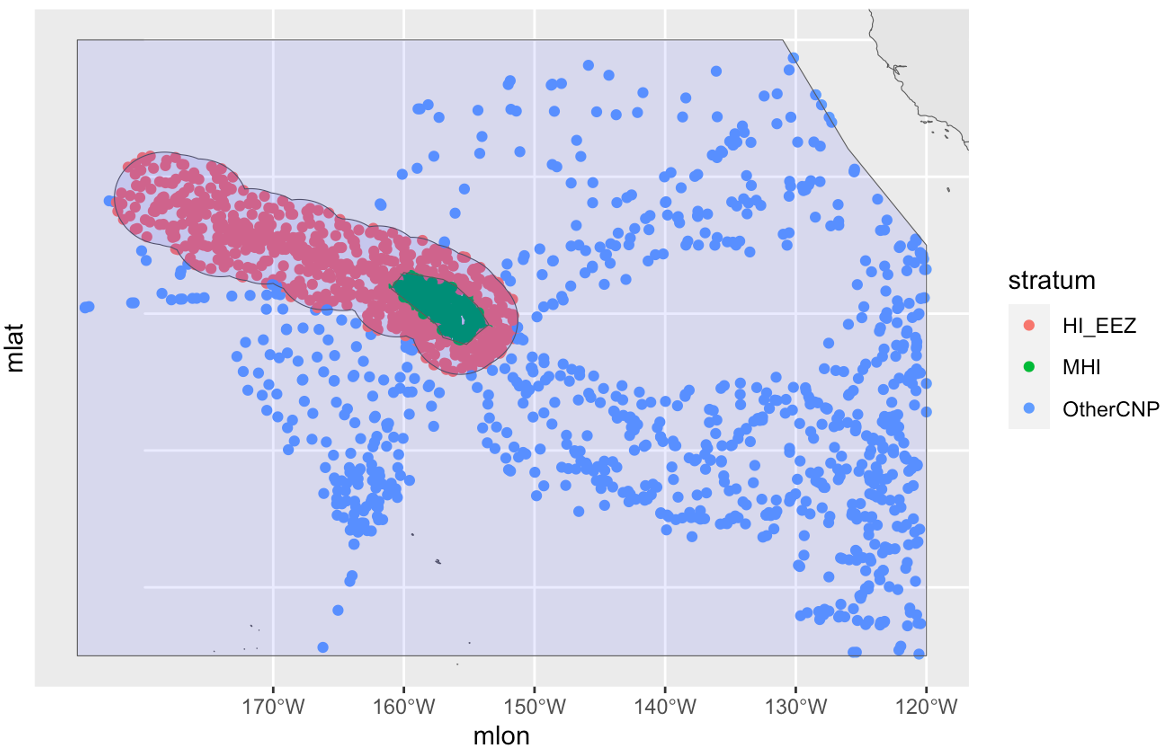
\includegraphics[width=0.75\textwidth,height=\textheight]{img/strata_overlap_hiceas.png}

Another option is \texttt{"each"}in which each time a stratum boundary is crossed the current segment will end and a new segment will begin. Also, stratum assignments for each row of effort will be shown as a concatenation of all the stratum layers overlapping at its position (e.g., ``OtherCNP\&HI\_EEZ''). Note that the \texttt{"each"} option segmentizes effort in the exact same was as \texttt{"smallest"} when strata are fully nested; its main advantage is in dealing with partially overlapping strata (such as strata used in the Marianas archipelago; see below).

The third option is \texttt{"largest"}, in which the largest of overlapping strata is used to assign a stratum name to each row. (We are not sure what use case this would serve, but we offer it as an option for niche analyses.)

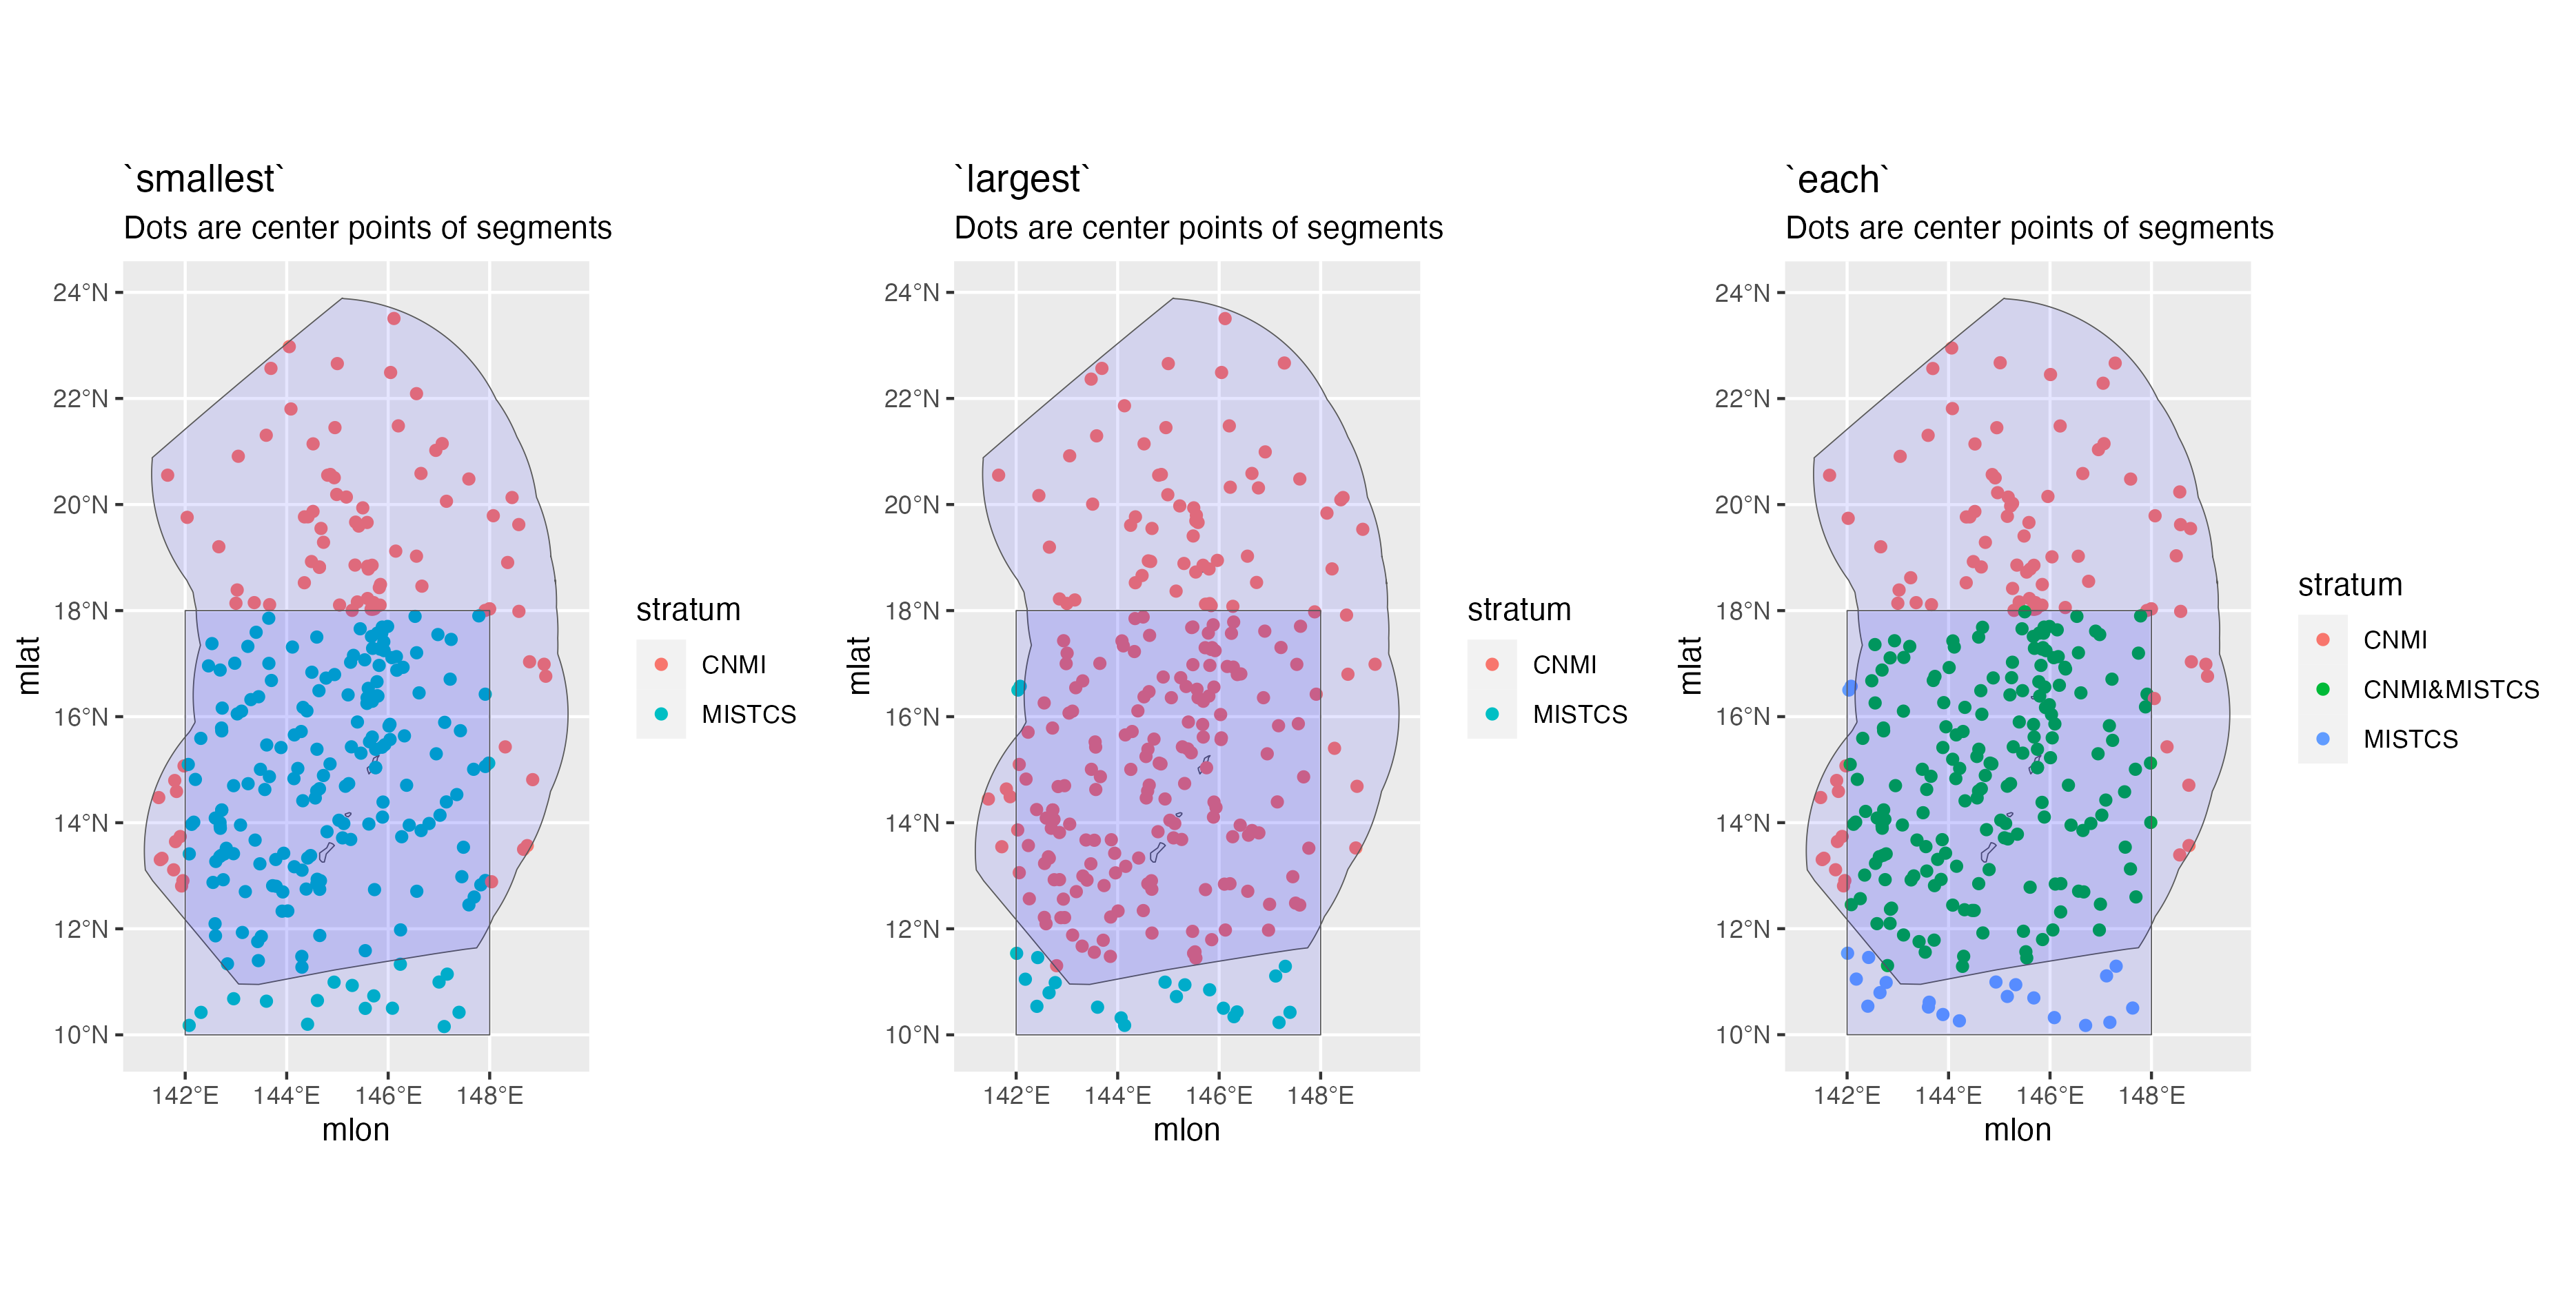
\includegraphics{img/strata_overlap_marianas.png}

\begin{itemize}
\item
  \textbf{\texttt{distance\_types:}} A character vector of the effort types that will be included in detection function estimation and density estimation, and therefore considered in effort segmentizing. Accepted values are \texttt{"S"} (systematic/standard effort), \texttt{"F"} (fine-scale effort), and \texttt{"N"} (non-systematic/non-standard effort, in which systematic protocols are being used but effort is not occurring along design-based transect routes). The default values are \texttt{c("S","F","N")}.
\item
  \textbf{\texttt{distance\_modes:}} The effort modes that will be included in detection function estimation and density estimation, and therefore considered in effort segmentizing. Accepted values are \texttt{"P"} (passing) and \texttt{"C"} (closing), and the default values are \texttt{c("P","C")}.
\item
  \textbf{\texttt{distance\_on\_off:}} The value(s) of \texttt{OnEffort} (On Effort is \texttt{TRUE}, Off Effort is \texttt{FALSE}) that will be included in detection function estimation and density estimation, and therefore considered in effort segmentizing. Default is \texttt{TRUE} only. (We don't expect \texttt{FALSE} or \texttt{c(TRUE,FALSE)} to be used much, if at all, but we make this option available).
\end{itemize}

\hypertarget{example-code}{%
\section*{Example code}\label{example-code}}
\addcontentsline{toc}{section}{Example code}

\hypertarget{use-settings-defaults}{%
\subsection*{Use settings defaults}\label{use-settings-defaults}}
\addcontentsline{toc}{subsection}{Use settings defaults}

No strata or group size calibration.

\begin{Shaded}
\begin{Highlighting}[]
\NormalTok{settings }\OtherTok{\textless{}{-}} \FunctionTok{load\_settings}\NormalTok{()}
\end{Highlighting}
\end{Shaded}

\hypertarget{use-settings-defaults-but-with-strata}{%
\subsection*{Use settings defaults, but with strata}\label{use-settings-defaults-but-with-strata}}
\addcontentsline{toc}{subsection}{Use settings defaults, but with strata}

\begin{Shaded}
\begin{Highlighting}[]
\CommentTok{\# Load strata dataframes}
\FunctionTok{data}\NormalTok{(strata\_cnp)}

\NormalTok{settings }\OtherTok{\textless{}{-}} \FunctionTok{load\_settings}\NormalTok{(}\AttributeTok{strata =}\NormalTok{ strata\_cnp)}
\end{Highlighting}
\end{Shaded}

\hypertarget{customize-survey-but-not-cohorts}{%
\subsection*{Customize survey, but not cohorts}\label{customize-survey-but-not-cohorts}}
\addcontentsline{toc}{subsection}{Customize survey, but not cohorts}

This code will process survey data such that effort segments are 5 km in length, with any effort falling outside of the provided geostrata relegated to a virtual geostratum named \texttt{"out"}. Since a cohort is not specified, the default values will be used.

\begin{Shaded}
\begin{Highlighting}[]
\CommentTok{\# Load built{-}in datasets}
\FunctionTok{data}\NormalTok{(strata\_cnp)}
\FunctionTok{data}\NormalTok{(group\_size\_coefficients)}
\FunctionTok{data}\NormalTok{(ships)}
\FunctionTok{data}\NormalTok{(species\_codes)}

\CommentTok{\# Survey settings}
\NormalTok{survey }\OtherTok{\textless{}{-}} 
  \FunctionTok{load\_survey\_settings}\NormalTok{(}\AttributeTok{out\_handling =} \StringTok{\textquotesingle{}stratum\textquotesingle{}}\NormalTok{,}
                       \AttributeTok{max\_row\_interval =} \DecValTok{700}\NormalTok{,}
                       \AttributeTok{segment\_method =} \StringTok{\textquotesingle{}equallength\textquotesingle{}}\NormalTok{,}
                       \AttributeTok{segment\_target\_km =} \DecValTok{5}\NormalTok{,}
                       \AttributeTok{segment\_max\_interval =}\NormalTok{ .}\DecValTok{3}\NormalTok{,}
                       \AttributeTok{segment\_remainder\_handling =} \FunctionTok{c}\NormalTok{(}\StringTok{\textquotesingle{}append\textquotesingle{}}\NormalTok{,}\StringTok{\textquotesingle{}segment\textquotesingle{}}\NormalTok{),}
                       \AttributeTok{ship\_list =}\NormalTok{ ships,}
                       \AttributeTok{species\_codes =}\NormalTok{ species\_codes,}
                       \AttributeTok{group\_size\_coefficients =}\NormalTok{ group\_size\_coefficients,}
                       \AttributeTok{smear\_angles =} \ConstantTok{FALSE}\NormalTok{)}

\CommentTok{\# Load settings}
\NormalTok{settings }\OtherTok{\textless{}{-}} \FunctionTok{load\_settings}\NormalTok{(}\AttributeTok{strata =}\NormalTok{ strata\_cnp,}
\NormalTok{                          survey)}
\end{Highlighting}
\end{Shaded}

\hypertarget{fully-custom-whiceas-case-study}{%
\subsection*{Fully custom: WHICEAS case study}\label{fully-custom-whiceas-case-study}}
\addcontentsline{toc}{subsection}{Fully custom: WHICEAS case study}

These are the settings we will use in the remainder of the tutorial.

\hypertarget{survey-wide-settings-1}{%
\subsubsection*{Survey-wide settings}\label{survey-wide-settings-1}}
\addcontentsline{toc}{subsubsection}{Survey-wide settings}

To emulate the analysis done in \href{https://repository.library.noaa.gov/view/noaa/47788}{Bradford et al.~(2021)}, we want to process effort with 150-km segments, relegating any remainder to its own segments. We also want to make sure to remove any survey data that falls outside of the geostrata, to ensure that detection functions are regionally specific. We will use the built-in tables for species codes, ship codes, and group size calibration coefficients.

\begin{Shaded}
\begin{Highlighting}[]
\FunctionTok{data}\NormalTok{(species\_codes)}
\FunctionTok{data}\NormalTok{(ships)}
\FunctionTok{data}\NormalTok{(group\_size\_coefficients)}

\NormalTok{survey }\OtherTok{\textless{}{-}} \FunctionTok{load\_survey\_settings}\NormalTok{(}
  \AttributeTok{out\_handling =} \StringTok{\textquotesingle{}remove\textquotesingle{}}\NormalTok{,}
  \AttributeTok{max\_row\_interval =} \ConstantTok{Inf}\NormalTok{,}
  \AttributeTok{segment\_method =} \StringTok{"equallength"}\NormalTok{,}
  \AttributeTok{segment\_target\_km =} \DecValTok{150}\NormalTok{,}
  \AttributeTok{segment\_max\_interval =} \DecValTok{24}\NormalTok{,}
  \AttributeTok{segment\_remainder\_handling =} \FunctionTok{c}\NormalTok{(}\StringTok{"segment"}\NormalTok{),}
  \AttributeTok{ship\_list =}\NormalTok{ ships,}
  \AttributeTok{species\_codes =}\NormalTok{ species\_codes,}
  \AttributeTok{group\_size\_coefficients =}\NormalTok{ group\_size\_coefficients,}
  \AttributeTok{smear\_angles =} \ConstantTok{FALSE}
\NormalTok{)}
\end{Highlighting}
\end{Shaded}

\hypertarget{geostrata}{%
\subsubsection*{Geostrata}\label{geostrata}}
\addcontentsline{toc}{subsubsection}{Geostrata}

We will use the built-in dataset of Central North Pacific geostrata:

\begin{Shaded}
\begin{Highlighting}[]
\FunctionTok{data}\NormalTok{(strata\_cnp)}
\NormalTok{strata\_cnp }\SpecialCharTok{\%\textgreater{}\%}\NormalTok{ names}
\NormalTok{ [}\DecValTok{1}\NormalTok{] }\StringTok{"HI\_EEZ"}          \StringTok{"OtherCNP"}        \StringTok{"MHI"}             \StringTok{"WHICEAS"}        
\NormalTok{ [}\DecValTok{5}\NormalTok{] }\StringTok{"Spotted\_OU"}      \StringTok{"Spotted\_FI"}      \StringTok{"Spotted\_BI"}      \StringTok{"Bottlenose\_KaNi"}
\NormalTok{ [}\DecValTok{9}\NormalTok{] }\StringTok{"Bottlenose\_OUFI"} \StringTok{"Bottlenose\_BI"}   \StringTok{"NWHI"}           
\end{Highlighting}
\end{Shaded}

\hypertarget{species-cohorts}{%
\subsubsection*{Species cohorts}\label{species-cohorts}}
\addcontentsline{toc}{subsubsection}{Species cohorts}

\textbf{Cohort 1: All species}\\
At least one cohort needs to be specified in order to run process survey data, so this first cohort will serve as a `catch-all' for species who do not need special handling. It does not hurt to include \emph{all} species in this catch-all cohort -- except perhaps by increasing the file-size of your processed data by a few kilobytes -- \emph{even if} you will be creating a separate, dedicated cohort for one of these species downstream. Having a catch-all cohort like this serves two purposes: (1) it avoids unforeseen complications if you will be modeling detection functions with multi-species pools, as mentioned above; and (2) it will simplify the code you will use to produce summary statistics of effort and sightings totals, since you will not need to pool together statistics from multiple cohorts.

To build this catch-all cohort, we will not specify any species so that \emph{all} species in the data are included, and we will specify that only the generic geostrata should be used, so that species specific insular stock boundaries are ignored.

Here we show all possible inputs. Most of these match the built-in defaults. Those that do not (there are just 3) are noted with a commented asterisk.

\begin{Shaded}
\begin{Highlighting}[]
\NormalTok{all\_species }\OtherTok{\textless{}{-}} \FunctionTok{load\_cohort\_settings}\NormalTok{(}
  \AttributeTok{id =} \StringTok{"all"}\NormalTok{, }\CommentTok{\# *}
  \AttributeTok{species =} \ConstantTok{NULL}\NormalTok{, }
  \AttributeTok{strata =} \FunctionTok{c}\NormalTok{(}\StringTok{\textquotesingle{}WHICEAS\textquotesingle{}}\NormalTok{, }\StringTok{\textquotesingle{}HI\_EEZ\textquotesingle{}}\NormalTok{, }\StringTok{\textquotesingle{}OtherCNP\textquotesingle{}}\NormalTok{), }\CommentTok{\# *}
  \AttributeTok{probable\_species =} \ConstantTok{FALSE}\NormalTok{,}
  \AttributeTok{sighting\_method =} \DecValTok{0}\NormalTok{,}
  \AttributeTok{cue\_range =} \DecValTok{0}\SpecialCharTok{:}\DecValTok{7}\NormalTok{,}
  \AttributeTok{school\_size\_range =} \FunctionTok{c}\NormalTok{(}\DecValTok{0}\NormalTok{, }\DecValTok{10000}\NormalTok{),}
  \AttributeTok{school\_size\_calibrate =} \ConstantTok{TRUE}\NormalTok{,}
  \AttributeTok{calibration\_floor =} \DecValTok{0}\NormalTok{,}
  \AttributeTok{use\_low\_if\_na =} \ConstantTok{TRUE}\NormalTok{,}
  \AttributeTok{io\_sightings =} \DecValTok{0}\NormalTok{,}
  \AttributeTok{geometric\_mean\_group =} \ConstantTok{TRUE}\NormalTok{,}
  \AttributeTok{truncation\_km =} \FloatTok{7.5}\NormalTok{, }\CommentTok{\# *}
  \AttributeTok{beaufort\_range =} \DecValTok{0}\SpecialCharTok{:}\DecValTok{6}\NormalTok{,}
  \AttributeTok{abeam\_sightings =} \ConstantTok{FALSE}\NormalTok{, }\CommentTok{\# *}
  \AttributeTok{strata\_overlap\_handling =} \FunctionTok{c}\NormalTok{(}\StringTok{"smallest"}\NormalTok{),}
  \AttributeTok{distance\_types =} \FunctionTok{c}\NormalTok{(}\StringTok{\textquotesingle{}S\textquotesingle{}}\NormalTok{,}\StringTok{\textquotesingle{}F\textquotesingle{}}\NormalTok{,}\StringTok{\textquotesingle{}N\textquotesingle{}}\NormalTok{),}
  \AttributeTok{distance\_modes =} \FunctionTok{c}\NormalTok{(}\StringTok{\textquotesingle{}P\textquotesingle{}}\NormalTok{,}\StringTok{\textquotesingle{}C\textquotesingle{}}\NormalTok{),}
  \AttributeTok{distance\_on\_off =} \ConstantTok{TRUE}
\NormalTok{)}
\end{Highlighting}
\end{Shaded}

\textbf{Cohort 2: Bottlenose dolphin}\\
As mentioned above, bottlenose dolphins are going to be analyzed as part of a multi-species pool that includes the rough-toothed dolphin, Risso's dolphin, and pygmy killer whale. Because those species' codes will be needed to model the detection function used in bottlenose dolphin density/abundance estimation, those species codes will be included in this cohort's settings.

Also mentioned above: Hawaii has a pelagic population of bottlenose dolphins as well as several distinct insular stocks. In this case study, we are interested in estimating only the abundance of the pelagic population, which means we will need to include geostrata of the insular stock boundaries in order to make sure the effort and sightings within those insular areas are ignored. That means we will specify the generic geostrata (\texttt{"WHICEAS"}, \texttt{"HI\_EEZ"}, and \texttt{"Other\_CNP"}), as well as the geostrata for the insular stocks.

We can spell out as many any inputs that we wish, but here will only show the inputs that are non-default and/or different from Cohort 1 above.

\begin{Shaded}
\begin{Highlighting}[]
\NormalTok{bottlenose }\OtherTok{\textless{}{-}} \FunctionTok{load\_cohort\_settings}\NormalTok{(}
  \AttributeTok{id =} \StringTok{"bottlenose"}\NormalTok{,}
  \AttributeTok{species =} \FunctionTok{c}\NormalTok{(}\StringTok{\textquotesingle{}015\textquotesingle{}}\NormalTok{, }\StringTok{\textquotesingle{}018\textquotesingle{}}\NormalTok{, }\StringTok{\textquotesingle{}021\textquotesingle{}}\NormalTok{, }\StringTok{\textquotesingle{}032\textquotesingle{}}\NormalTok{),}
  \AttributeTok{strata =} \FunctionTok{c}\NormalTok{(}\StringTok{\textquotesingle{}WHICEAS\textquotesingle{}}\NormalTok{, }\StringTok{\textquotesingle{}HI\_EEZ\textquotesingle{}}\NormalTok{, }\StringTok{\textquotesingle{}OtherCNP\textquotesingle{}}\NormalTok{,}
             \StringTok{\textquotesingle{}Bottlenose\_BI\textquotesingle{}}\NormalTok{, }\StringTok{\textquotesingle{}Bottlenose\_OUFI\textquotesingle{}}\NormalTok{, }\StringTok{\textquotesingle{}Bottlenose\_KaNi\textquotesingle{}}\NormalTok{),}
  \AttributeTok{truncation\_km =} \FloatTok{7.5}\NormalTok{)}
\end{Highlighting}
\end{Shaded}

\textbf{Cohort 3: Pantropical spotted dolphin}\\
Similar to the bottlenose dolphin above, spotted dolphins in Hawaiian waters belong to pelagic stocks as well as insular stocks. We will be estimating density/abundance for the only pelagic stocks here, but we need to include the geostrata for the insular stocks in order to ignore their effort and sightings.

\begin{Shaded}
\begin{Highlighting}[]
\NormalTok{spotted }\OtherTok{\textless{}{-}} \FunctionTok{load\_cohort\_settings}\NormalTok{(}
  \AttributeTok{id =} \StringTok{"spotted"}\NormalTok{,}
  \AttributeTok{species =} \StringTok{\textquotesingle{}002\textquotesingle{}}\NormalTok{,}
  \AttributeTok{strata =} \FunctionTok{c}\NormalTok{(}\StringTok{\textquotesingle{}WHICEAS\textquotesingle{}}\NormalTok{, }\StringTok{\textquotesingle{}HI\_EEZ\textquotesingle{}}\NormalTok{, }\StringTok{\textquotesingle{}OtherCNP\textquotesingle{}}\NormalTok{,}
             \StringTok{\textquotesingle{}Spotted\_OU\textquotesingle{}}\NormalTok{,}\StringTok{\textquotesingle{}Spotted\_FI\textquotesingle{}}\NormalTok{,}\StringTok{\textquotesingle{}Spotted\_BI\textquotesingle{}}\NormalTok{),}
  \AttributeTok{truncation\_km =} \FloatTok{7.5}\NormalTok{)}
\end{Highlighting}
\end{Shaded}

\hypertarget{compile-settings}{%
\subsubsection*{Compile settings}\label{compile-settings}}
\addcontentsline{toc}{subsubsection}{Compile settings}

Finally, we create our \texttt{settings} object, providing \texttt{cohorts} as a list of lists:

\begin{Shaded}
\begin{Highlighting}[]
\NormalTok{settings }\OtherTok{\textless{}{-}} \FunctionTok{load\_settings}\NormalTok{(}\AttributeTok{strata =}\NormalTok{ strata\_cnp,}
                          \AttributeTok{survey =}\NormalTok{ survey,}
                          \AttributeTok{cohorts =} \FunctionTok{list}\NormalTok{(all\_species,}
\NormalTok{                                         bottlenose,}
\NormalTok{                                         spotted))}
\end{Highlighting}
\end{Shaded}

Save this \texttt{settings} object locally, to use in downstream scripts:

\begin{Shaded}
\begin{Highlighting}[]
\FunctionTok{save}\NormalTok{(settings, }\AttributeTok{file=}\StringTok{\textquotesingle{}whiceas\_settings.RData\textquotesingle{}}\NormalTok{)}
\end{Highlighting}
\end{Shaded}

\hypertarget{das}{%
\chapter{DAS editing}\label{das}}

The \texttt{LTabundR} package includes several functions that facilitate the exploration of \texttt{DAS} files of \texttt{WinCruz} survey data, as well as a function that allows you to apply ``edits'' to the survey data in a reproducible way (i.e., using code, without modifying the actual data file).

\hypertarget{reviewing-a-das-file}{%
\section*{\texorpdfstring{Reviewing a \texttt{DAS} file}{Reviewing a DAS file}}\label{reviewing-a-das-file}}
\addcontentsline{toc}{section}{Reviewing a \texttt{DAS} file}

\hypertarget{das_readtext}{%
\subsection*{\texorpdfstring{\texttt{das\_readtext()}}{das\_readtext()}}\label{das_readtext}}
\addcontentsline{toc}{subsection}{\texttt{das\_readtext()}}

The \texttt{swfscDAS} package has functions for reading in a \texttt{DAS} file and parsing it into columns of fixed-width text. To complement those functions, \texttt{LTabundR} includes the function \texttt{das\_readtext()}, which reads in a \texttt{DAS} file without applying any column parsing, so that the data can be read in its true raw format.

\begin{Shaded}
\begin{Highlighting}[]
\CommentTok{\# Local path to DAS file}
\NormalTok{das\_file }\OtherTok{\textless{}{-}} \StringTok{\textquotesingle{}data/surveys/CenPac1986{-}2020\_Final\_alb.das\textquotesingle{}}

\NormalTok{das }\OtherTok{\textless{}{-}} \FunctionTok{das\_readtext}\NormalTok{(das\_file)}
\NormalTok{das}\SpecialCharTok{$}\NormalTok{das }\SpecialCharTok{\%\textgreater{}\%} \FunctionTok{head}\NormalTok{(}\DecValTok{20}\NormalTok{)}
\NormalTok{ [}\DecValTok{1}\NormalTok{] }\StringTok{"  1B 1805   073086 N31:57.   W116:57.    989"}                                   
\NormalTok{ [}\DecValTok{2}\NormalTok{] }\StringTok{"  1S 1805   073086 N31:57.   W116:57.     01  004    6    4  300 1.77  1.5"}     
\NormalTok{ [}\DecValTok{3}\NormalTok{] }\StringTok{"  2A 1805   073086 N31:57.   W116:57.     01 15.0         N  099"}               
\NormalTok{ [}\DecValTok{4}\NormalTok{] }\StringTok{"   1                                     004 0001 0001 0001  100  000  000  000"}
\NormalTok{ [}\DecValTok{5}\NormalTok{] }\StringTok{"  1S 0610   073186 N30:05.   W116:04.     01  004    3    4  340 5.00  0.1"}     
\NormalTok{ [}\DecValTok{6}\NormalTok{] }\StringTok{"  2A 0610   073186 N30:05.   W116:04.     01 18.3         N  005"}               
\NormalTok{ [}\DecValTok{7}\NormalTok{] }\StringTok{"   1                                     004 0150 0175 0125  100  000  000  000"}
\NormalTok{ [}\DecValTok{8}\NormalTok{] }\StringTok{"  3B.1311   073186 N29:46.   W115:52.    989              N"}                    
\NormalTok{ [}\DecValTok{9}\NormalTok{] }\StringTok{"  4R.1311   073186 N29:46.   W115:52.      N"}                                   
\NormalTok{[}\DecValTok{10}\NormalTok{] }\StringTok{"  5P.1311   073186 N29:46.   W115:52.    022  031  056"}                         
\NormalTok{[}\DecValTok{11}\NormalTok{] }\StringTok{"  6V.1311   073186 N29:46.   W115:52.      4           16.1"}                    
\NormalTok{[}\DecValTok{12}\NormalTok{] }\StringTok{"  7N.1311   073186 N29:46.   W115:52.    167 10.5"}                              
\NormalTok{[}\DecValTok{13}\NormalTok{] }\StringTok{"  8W.1311   073186 N29:46.   W115:52.      2"}                                   
\NormalTok{[}\DecValTok{14}\NormalTok{] }\StringTok{"  9V.1329   073186 N29:43.   W115:51.      5           16.1"}                    
\NormalTok{[}\DecValTok{15}\NormalTok{] }\StringTok{" 10P.1404   073186 N29:37.   W115:50.    004  056  062"}                         
\NormalTok{[}\DecValTok{16}\NormalTok{] }\StringTok{" 11V.1404   073186 N29:37.   W115:50.      5           18.3"}                    
\NormalTok{[}\DecValTok{17}\NormalTok{] }\StringTok{" 12S.1406   073186 N29:37.   W115:50.     02  004    3    4  355  1.4  1.8"}     
\NormalTok{[}\DecValTok{18}\NormalTok{] }\StringTok{" 13A.1406   073186 N29:37.   W115:50.     02 18.3         Y  005"}               
\NormalTok{[}\DecValTok{19}\NormalTok{] }\StringTok{"   1                                     022 0030 0100 0020  100  000  000  000"}
\NormalTok{[}\DecValTok{20}\NormalTok{] }\StringTok{"   2                                     004 0250 0300 0200  100  000  000  000"}
\end{Highlighting}
\end{Shaded}

To follow along, this data file can be downloaded \href{https://raw.githubusercontent.com/emk-noaa/LTAvignette/main/data/surveys/CenPac1986-2020_Final_alb.das?token=GHSAT0AAAAAACFPESQVLR7DOE4I3UD4UJ2YZGRILEQ}{here}.

\hypertarget{das_inspector}{%
\subsection*{\texorpdfstring{\texttt{das\_inspector()}}{das\_inspector()}}\label{das_inspector}}
\addcontentsline{toc}{subsection}{\texttt{das\_inspector()}}

We also provide a function, \texttt{das\_inspector()}, that allows you to explore a \texttt{DAS} file within an interactive \texttt{Shiny} app. This app can also be used to find, prepare, and preview coded edits to the \texttt{DAS} data.

\begin{Shaded}
\begin{Highlighting}[]
\FunctionTok{das\_inspector}\NormalTok{(das\_file)}
\end{Highlighting}
\end{Shaded}

In this app, you specify the rows and `columns' (i.e., character indices) that will be affected by your edit, the edit you want to apply, and the type of edit it will be (see next subsection). You then ``save'' that edit with the click of a button, and when you close the app your log of staged edits will be returned as a \texttt{list}. You can then pass this list of edits to \texttt{das\_editor()} (next subsection on this page), or as an argument within \texttt{process\_surveys()} (next page).

\hypertarget{staging-edits}{%
\section*{Staging edits}\label{staging-edits}}
\addcontentsline{toc}{section}{Staging edits}

The \texttt{das\_editor()} function allows you to apply edits to a \texttt{DAS} file without modifiyng the original data. You supply edits to this function as a set of instructions saved within a \texttt{list} object. You can prepare these instructions manually or use the \texttt{das\_inspector()} function above to get help. The \texttt{das\_editor()} function then loops through each edit, applies them to a local version of the data, and returns that modified data to the user. This allows survey data to be modified reproducibly before being processed with \texttt{LTabundR::process\_surveys()} without touching the original \texttt{DAS} data files or requiring analysts to duplicate files and make one-off modifications manually.

We expect it would be rare for a user to call \texttt{das\_editor()} directly; instead, they would supply their edits as an argument in \texttt{process\_surveys()}, and that function will call \texttt{das\_editor()} internally to amend the survey data before it is processed (this is discussed on the next page).

Note that there is no limit to the number of edits that can be provided in a single \texttt{list}, and they can be provided in any order. The \texttt{das\_editor()} function will sort the edits by \texttt{DAS} file and by edit type, and then apply edits in increasing order of ``disruption'', i.e., text replacements first, then moving rows of data (no net change in number of rows), then copying-pasting, inserting, and deleting.

The \texttt{das\_editor()} function can currently handle 6 types of edits, which we shall demonstrate below.

\hypertarget{types-of-editing}{%
\subsection*{Types of editing}\label{types-of-editing}}
\addcontentsline{toc}{subsection}{Types of editing}

To demonstrate the types of editing actions that can be achieved through \texttt{das\_editor()}, we will use the \texttt{DAS} file from the 2020 WHICEAS survey (you can download \href{https://raw.githubusercontent.com/emk-noaa/LTAvignette/main/data/surveys/HICEASwinter2020.das?token=GHSAT0AAAAAACFPESQVZWKAJE3NCRQBC4SCZGRJNLA}{here}).

\begin{Shaded}
\begin{Highlighting}[]
\CommentTok{\# Local path to das\_file}
\NormalTok{das\_file }\OtherTok{\textless{}{-}} \StringTok{"data/surveys/HICEASwinter2020.das"}
\NormalTok{das }\OtherTok{\textless{}{-}} \FunctionTok{das\_readtext}\NormalTok{(das\_file)}
\end{Highlighting}
\end{Shaded}

\hypertarget{verbatim-text-replacement}{%
\subsubsection*{Verbatim text replacement}\label{verbatim-text-replacement}}
\addcontentsline{toc}{subsubsection}{Verbatim text replacement}

The \texttt{edit} will be interpreted verbatim as text that will replace the specified data.

\begin{Shaded}
\begin{Highlighting}[]
\NormalTok{edits }\OtherTok{\textless{}{-}} \FunctionTok{list}\NormalTok{(}\FunctionTok{list}\NormalTok{(}\AttributeTok{das\_file =}\NormalTok{ das\_file, }
                   \AttributeTok{type =} \StringTok{\textquotesingle{}text\textquotesingle{}}\NormalTok{,}
                   \AttributeTok{rows =} \DecValTok{10}\SpecialCharTok{:}\DecValTok{15}\NormalTok{, }
                   \AttributeTok{chars =} \DecValTok{20}\SpecialCharTok{:}\DecValTok{39}\NormalTok{, }
                   \AttributeTok{edit =} \StringTok{\textquotesingle{}lat, lon\textquotesingle{}}\NormalTok{))}
\end{Highlighting}
\end{Shaded}

Here is what this edit log object will look like:

\begin{Shaded}
\begin{Highlighting}[]
\NormalTok{edits}
\NormalTok{[[}\DecValTok{1}\NormalTok{]]}
\NormalTok{[[}\DecValTok{1}\NormalTok{]]}\SpecialCharTok{$}\NormalTok{das\_file}
\NormalTok{[}\DecValTok{1}\NormalTok{] }\StringTok{"data/surveys/HICEASwinter2020.das"}

\NormalTok{[[}\DecValTok{1}\NormalTok{]]}\SpecialCharTok{$}\NormalTok{type}
\NormalTok{[}\DecValTok{1}\NormalTok{] }\StringTok{"text"}

\NormalTok{[[}\DecValTok{1}\NormalTok{]]}\SpecialCharTok{$}\NormalTok{rows}
\NormalTok{[}\DecValTok{1}\NormalTok{] }\DecValTok{10} \DecValTok{11} \DecValTok{12} \DecValTok{13} \DecValTok{14} \DecValTok{15}

\NormalTok{[[}\DecValTok{1}\NormalTok{]]}\SpecialCharTok{$}\NormalTok{chars}
\NormalTok{ [}\DecValTok{1}\NormalTok{] }\DecValTok{20} \DecValTok{21} \DecValTok{22} \DecValTok{23} \DecValTok{24} \DecValTok{25} \DecValTok{26} \DecValTok{27} \DecValTok{28} \DecValTok{29} \DecValTok{30} \DecValTok{31} \DecValTok{32} \DecValTok{33} \DecValTok{34} \DecValTok{35} \DecValTok{36} \DecValTok{37} \DecValTok{38} \DecValTok{39}

\NormalTok{[[}\DecValTok{1}\NormalTok{]]}\SpecialCharTok{$}\NormalTok{edit}
\NormalTok{[}\DecValTok{1}\NormalTok{] }\StringTok{"lat, lon"}
\end{Highlighting}
\end{Shaded}

And here is the effect it will have:

\begin{Shaded}
\begin{Highlighting}[]
\CommentTok{\# Before}
\NormalTok{das}\SpecialCharTok{$}\NormalTok{das[}\DecValTok{9}\SpecialCharTok{:}\DecValTok{16}\NormalTok{]}
\NormalTok{[}\DecValTok{1}\NormalTok{] }\StringTok{"009* 072752 011920 N21:50.58 W159:46.26"}                         
\NormalTok{[}\DecValTok{2}\NormalTok{] }\StringTok{"010* 072952 011920 N21:50.91 W159:46.33"}                         
\NormalTok{[}\DecValTok{3}\NormalTok{] }\StringTok{"011B.073111 011920 N21:51.12 W159:46.36 2001    C  {-}10    N"}     
\NormalTok{[}\DecValTok{4}\NormalTok{] }\StringTok{"012R.073111 011920 N21:51.12 W159:46.36    F"}                    
\NormalTok{[}\DecValTok{5}\NormalTok{] }\StringTok{"013P.073111 011920 N21:51.12 W159:46.36  126  307  238     "}     
\NormalTok{[}\DecValTok{6}\NormalTok{] }\StringTok{"014V.073111 011920 N21:51.12 W159:46.36    4   06  120      15.0"}
\NormalTok{[}\DecValTok{7}\NormalTok{] }\StringTok{"015N.073111 011920 N21:51.12 W159:46.36  350 09.9"}               
\NormalTok{[}\DecValTok{8}\NormalTok{] }\StringTok{"016W.073111 011920 N21:51.12 W159:46.36    5            120  6.0"}

\CommentTok{\# After}
\NormalTok{dase }\OtherTok{\textless{}{-}} \FunctionTok{das\_editor}\NormalTok{(edits)}
\NormalTok{Applying edits to DAS file}\SpecialCharTok{:}\NormalTok{ data}\SpecialCharTok{/}\NormalTok{surveys}\SpecialCharTok{/}\NormalTok{HICEASwinter2020.das}
\SpecialCharTok{{-}{-}{-}}\NormalTok{ verbatim}\SpecialCharTok{/}\ControlFlowTok{function}\NormalTok{ text replacements ...}
\SpecialCharTok{{-}{-}{-}} \SpecialCharTok{{-}{-}{-}}\NormalTok{ working on edit }\DecValTok{1}\NormalTok{ ...}
\NormalTok{dase}\SpecialCharTok{$}\NormalTok{das[[}\DecValTok{1}\NormalTok{]]}\SpecialCharTok{$}\NormalTok{das}\SpecialCharTok{$}\NormalTok{das[}\DecValTok{9}\SpecialCharTok{:}\DecValTok{16}\NormalTok{]}
\NormalTok{[}\DecValTok{1}\NormalTok{] }\StringTok{"009* 072752 011920 N21:50.58 W159:46.26"}                         
\NormalTok{[}\DecValTok{2}\NormalTok{] }\StringTok{"010* 072952 011920 lat, lon"}                                     
\NormalTok{[}\DecValTok{3}\NormalTok{] }\StringTok{"011B.073111 011920 lat, lon 2001    C  {-}10    N"}                 
\NormalTok{[}\DecValTok{4}\NormalTok{] }\StringTok{"012R.073111 011920 lat, lon    F"}                                
\NormalTok{[}\DecValTok{5}\NormalTok{] }\StringTok{"013P.073111 011920 lat, lon  126  307  238     "}                 
\NormalTok{[}\DecValTok{6}\NormalTok{] }\StringTok{"014V.073111 011920 lat, lon    4   06  120      15.0"}            
\NormalTok{[}\DecValTok{7}\NormalTok{] }\StringTok{"015N.073111 011920 lat, lon  350 09.9"}                           
\NormalTok{[}\DecValTok{8}\NormalTok{] }\StringTok{"016W.073111 011920 N21:51.12 W159:46.36    5            120  6.0"}
\end{Highlighting}
\end{Shaded}

\hypertarget{function-based-text-replacement}{%
\subsubsection*{Function-based text replacement}\label{function-based-text-replacement}}
\addcontentsline{toc}{subsubsection}{Function-based text replacement}

The \texttt{edit} will be evaluated as a function that is applied to the specified characters in each of \texttt{rows}.

\begin{Shaded}
\begin{Highlighting}[]
\NormalTok{edits }\OtherTok{\textless{}{-}} \FunctionTok{list}\NormalTok{(}\FunctionTok{list}\NormalTok{(}\AttributeTok{das\_file =}\NormalTok{ das\_file, }
                   \AttributeTok{type =} \StringTok{\textquotesingle{}function\textquotesingle{}}\NormalTok{,}
                   \AttributeTok{rows =} \DecValTok{10}\SpecialCharTok{:}\DecValTok{15}\NormalTok{, }
                   \AttributeTok{chars =} \DecValTok{20}\SpecialCharTok{:}\DecValTok{39}\NormalTok{, }
                   \AttributeTok{edit =} \StringTok{\textquotesingle{}tolower\textquotesingle{}}\NormalTok{))}

\CommentTok{\# Before}
\NormalTok{das}\SpecialCharTok{$}\NormalTok{das[}\DecValTok{9}\SpecialCharTok{:}\DecValTok{16}\NormalTok{]}
\NormalTok{[}\DecValTok{1}\NormalTok{] }\StringTok{"009* 072752 011920 N21:50.58 W159:46.26"}                         
\NormalTok{[}\DecValTok{2}\NormalTok{] }\StringTok{"010* 072952 011920 N21:50.91 W159:46.33"}                         
\NormalTok{[}\DecValTok{3}\NormalTok{] }\StringTok{"011B.073111 011920 N21:51.12 W159:46.36 2001    C  {-}10    N"}     
\NormalTok{[}\DecValTok{4}\NormalTok{] }\StringTok{"012R.073111 011920 N21:51.12 W159:46.36    F"}                    
\NormalTok{[}\DecValTok{5}\NormalTok{] }\StringTok{"013P.073111 011920 N21:51.12 W159:46.36  126  307  238     "}     
\NormalTok{[}\DecValTok{6}\NormalTok{] }\StringTok{"014V.073111 011920 N21:51.12 W159:46.36    4   06  120      15.0"}
\NormalTok{[}\DecValTok{7}\NormalTok{] }\StringTok{"015N.073111 011920 N21:51.12 W159:46.36  350 09.9"}               
\NormalTok{[}\DecValTok{8}\NormalTok{] }\StringTok{"016W.073111 011920 N21:51.12 W159:46.36    5            120  6.0"}

\CommentTok{\# After}
\NormalTok{dase }\OtherTok{\textless{}{-}} \FunctionTok{das\_editor}\NormalTok{(edits)}
\NormalTok{Applying edits to DAS file}\SpecialCharTok{:}\NormalTok{ data}\SpecialCharTok{/}\NormalTok{surveys}\SpecialCharTok{/}\NormalTok{HICEASwinter2020.das}
\SpecialCharTok{{-}{-}{-}}\NormalTok{ verbatim}\SpecialCharTok{/}\ControlFlowTok{function}\NormalTok{ text replacements ...}
\SpecialCharTok{{-}{-}{-}} \SpecialCharTok{{-}{-}{-}}\NormalTok{ working on edit }\DecValTok{1}\NormalTok{ ...}
\NormalTok{dase}\SpecialCharTok{$}\NormalTok{das[[}\DecValTok{1}\NormalTok{]]}\SpecialCharTok{$}\NormalTok{das}\SpecialCharTok{$}\NormalTok{das[}\DecValTok{9}\SpecialCharTok{:}\DecValTok{16}\NormalTok{]}
\NormalTok{[}\DecValTok{1}\NormalTok{] }\StringTok{"009* 072752 011920 N21:50.58 W159:46.26"}                         
\NormalTok{[}\DecValTok{2}\NormalTok{] }\StringTok{"010* 072952 011920 n21:50.91 w159:46.33"}                         
\NormalTok{[}\DecValTok{3}\NormalTok{] }\StringTok{"011B.073111 011920 n21:51.12 w159:46.36 2001    C  {-}10    N"}     
\NormalTok{[}\DecValTok{4}\NormalTok{] }\StringTok{"012R.073111 011920 n21:51.12 w159:46.36    F"}                    
\NormalTok{[}\DecValTok{5}\NormalTok{] }\StringTok{"013P.073111 011920 n21:51.12 w159:46.36  126  307  238     "}     
\NormalTok{[}\DecValTok{6}\NormalTok{] }\StringTok{"014V.073111 011920 n21:51.12 w159:46.36    4   06  120      15.0"}
\NormalTok{[}\DecValTok{7}\NormalTok{] }\StringTok{"015N.073111 011920 n21:51.12 w159:46.36  350 09.9"}               
\NormalTok{[}\DecValTok{8}\NormalTok{] }\StringTok{"016W.073111 011920 N21:51.12 W159:46.36    5            120  6.0"}
\end{Highlighting}
\end{Shaded}

A special application of this form of editing is adjusting timestamps using the \texttt{LTabundR} function \texttt{das\_time()}. In this next example, we subtract an hour from the first 5 rows of timestamps:

\begin{Shaded}
\begin{Highlighting}[]
\NormalTok{edits }\OtherTok{\textless{}{-}} \FunctionTok{list}\NormalTok{(}\FunctionTok{list}\NormalTok{(}\AttributeTok{das\_file =}\NormalTok{ das\_file, }
                   \AttributeTok{type =} \StringTok{\textquotesingle{}function\textquotesingle{}}\NormalTok{,}
                   \AttributeTok{rows =} \DecValTok{1}\SpecialCharTok{:}\DecValTok{5}\NormalTok{, }
                   \AttributeTok{chars =} \DecValTok{6}\SpecialCharTok{:}\DecValTok{40}\NormalTok{, }
                   \AttributeTok{edit =} \StringTok{\textquotesingle{}function(x)\{das\_time(x, tz\_adjust = {-}1)$dt\}\textquotesingle{}}\NormalTok{))}

\CommentTok{\# Before}
\NormalTok{das}\SpecialCharTok{$}\NormalTok{das[}\DecValTok{1}\SpecialCharTok{:}\DecValTok{6}\NormalTok{]}
\NormalTok{[}\DecValTok{1}\NormalTok{] }\StringTok{"001* 071152 011920 N21:47.99 W159:45.91"}
\NormalTok{[}\DecValTok{2}\NormalTok{] }\StringTok{"002* 071352 011920 N21:48.31 W159:45.94"}
\NormalTok{[}\DecValTok{3}\NormalTok{] }\StringTok{"003* 071552 011920 N21:48.63 W159:45.97"}
\NormalTok{[}\DecValTok{4}\NormalTok{] }\StringTok{"004* 071752 011920 N21:48.95 W159:46.01"}
\NormalTok{[}\DecValTok{5}\NormalTok{] }\StringTok{"005* 071952 011920 N21:49.28 W159:46.04"}
\NormalTok{[}\DecValTok{6}\NormalTok{] }\StringTok{"006* 072152 011920 N21:49.60 W159:46.08"}

\CommentTok{\# After}
\NormalTok{dase }\OtherTok{\textless{}{-}} \FunctionTok{das\_editor}\NormalTok{(edits)}
\NormalTok{Applying edits to DAS file}\SpecialCharTok{:}\NormalTok{ data}\SpecialCharTok{/}\NormalTok{surveys}\SpecialCharTok{/}\NormalTok{HICEASwinter2020.das}
\SpecialCharTok{{-}{-}{-}}\NormalTok{ verbatim}\SpecialCharTok{/}\ControlFlowTok{function}\NormalTok{ text replacements ...}
\SpecialCharTok{{-}{-}{-}} \SpecialCharTok{{-}{-}{-}}\NormalTok{ working on edit }\DecValTok{1}\NormalTok{ ...}
\NormalTok{dase}\SpecialCharTok{$}\NormalTok{das[[}\DecValTok{1}\NormalTok{]]}\SpecialCharTok{$}\NormalTok{das}\SpecialCharTok{$}\NormalTok{das[}\DecValTok{1}\SpecialCharTok{:}\DecValTok{6}\NormalTok{]}
\NormalTok{[}\DecValTok{1}\NormalTok{] }\StringTok{"001* 061152 011920 N21:47.99 W159:45.91"}
\NormalTok{[}\DecValTok{2}\NormalTok{] }\StringTok{"002* 061352 011920 N21:48.31 W159:45.94"}
\NormalTok{[}\DecValTok{3}\NormalTok{] }\StringTok{"003* 061552 011920 N21:48.63 W159:45.97"}
\NormalTok{[}\DecValTok{4}\NormalTok{] }\StringTok{"004* 061752 011920 N21:48.95 W159:46.01"}
\NormalTok{[}\DecValTok{5}\NormalTok{] }\StringTok{"005* 061952 011920 N21:49.28 W159:46.04"}
\NormalTok{[}\DecValTok{6}\NormalTok{] }\StringTok{"006* 072152 011920 N21:49.60 W159:46.08"}
\end{Highlighting}
\end{Shaded}

In the event that a survey was conducted using UTC timestamps instead of local time, you can adjust each timestamp according to its actual timezone as determined from its corresponding lat/long coordinates. Let's say the first 5 timestamps were collected in UTC by accident. The following code could correct that mistake:

\begin{Shaded}
\begin{Highlighting}[]
\NormalTok{edits }\OtherTok{\textless{}{-}} \FunctionTok{list}\NormalTok{(}\FunctionTok{list}\NormalTok{(}\AttributeTok{das\_file =}\NormalTok{ das\_file, }
                   \AttributeTok{type =} \StringTok{\textquotesingle{}function\textquotesingle{}}\NormalTok{,}
                   \AttributeTok{rows =} \DecValTok{1}\SpecialCharTok{:}\DecValTok{5}\NormalTok{, }
                   \AttributeTok{chars =} \DecValTok{6}\SpecialCharTok{:}\DecValTok{40}\NormalTok{, }
                   \AttributeTok{edit =} \StringTok{\textquotesingle{}function(x)\{das\_time(x, tz\_adjust = "from utc")$dt\}\textquotesingle{}}\NormalTok{))}

\CommentTok{\# Before}
\NormalTok{das}\SpecialCharTok{$}\NormalTok{das[}\DecValTok{1}\SpecialCharTok{:}\DecValTok{6}\NormalTok{]}
\NormalTok{[}\DecValTok{1}\NormalTok{] }\StringTok{"001* 071152 011920 N21:47.99 W159:45.91"}
\NormalTok{[}\DecValTok{2}\NormalTok{] }\StringTok{"002* 071352 011920 N21:48.31 W159:45.94"}
\NormalTok{[}\DecValTok{3}\NormalTok{] }\StringTok{"003* 071552 011920 N21:48.63 W159:45.97"}
\NormalTok{[}\DecValTok{4}\NormalTok{] }\StringTok{"004* 071752 011920 N21:48.95 W159:46.01"}
\NormalTok{[}\DecValTok{5}\NormalTok{] }\StringTok{"005* 071952 011920 N21:49.28 W159:46.04"}
\NormalTok{[}\DecValTok{6}\NormalTok{] }\StringTok{"006* 072152 011920 N21:49.60 W159:46.08"}

\CommentTok{\# After}
\NormalTok{dase }\OtherTok{\textless{}{-}} \FunctionTok{das\_editor}\NormalTok{(edits)}
\NormalTok{Applying edits to DAS file}\SpecialCharTok{:}\NormalTok{ data}\SpecialCharTok{/}\NormalTok{surveys}\SpecialCharTok{/}\NormalTok{HICEASwinter2020.das}
\SpecialCharTok{{-}{-}{-}}\NormalTok{ verbatim}\SpecialCharTok{/}\ControlFlowTok{function}\NormalTok{ text replacements ...}
\SpecialCharTok{{-}{-}{-}} \SpecialCharTok{{-}{-}{-}}\NormalTok{ working on edit }\DecValTok{1}\NormalTok{ ...}
\NormalTok{dase}\SpecialCharTok{$}\NormalTok{das[[}\DecValTok{1}\NormalTok{]]}\SpecialCharTok{$}\NormalTok{das}\SpecialCharTok{$}\NormalTok{das[}\DecValTok{1}\SpecialCharTok{:}\DecValTok{6}\NormalTok{]}
\NormalTok{[}\DecValTok{1}\NormalTok{] }\StringTok{"001* 201152 011820 N21:47.99 W159:45.91"}
\NormalTok{[}\DecValTok{2}\NormalTok{] }\StringTok{"002* 201352 011820 N21:48.31 W159:45.94"}
\NormalTok{[}\DecValTok{3}\NormalTok{] }\StringTok{"003* 201552 011820 N21:48.63 W159:45.97"}
\NormalTok{[}\DecValTok{4}\NormalTok{] }\StringTok{"004* 201752 011820 N21:48.95 W159:46.01"}
\NormalTok{[}\DecValTok{5}\NormalTok{] }\StringTok{"005* 201952 011820 N21:49.28 W159:46.04"}
\NormalTok{[}\DecValTok{6}\NormalTok{] }\StringTok{"006* 072152 011920 N21:49.60 W159:46.08"}
\end{Highlighting}
\end{Shaded}

\hypertarget{moving-data}{%
\subsubsection*{Moving data}\label{moving-data}}
\addcontentsline{toc}{subsubsection}{Moving data}

The \texttt{rows} will be deleted from their current location and pasted immediately below the row number specified by \texttt{edit}. The moved rows will be given the same date, time, latitude, and longitude, as the \texttt{edit} row.

\begin{Shaded}
\begin{Highlighting}[]
\NormalTok{edits }\OtherTok{\textless{}{-}} \FunctionTok{list}\NormalTok{(}\FunctionTok{list}\NormalTok{(}\AttributeTok{das\_file =}\NormalTok{ das\_file, }
                    \AttributeTok{type =} \StringTok{\textquotesingle{}move\textquotesingle{}}\NormalTok{,}
                    \AttributeTok{rows =} \DecValTok{10}\NormalTok{, }
                    \AttributeTok{chars =} \ConstantTok{NULL}\NormalTok{, }
                    \AttributeTok{edit =} \DecValTok{15}\NormalTok{))}

\CommentTok{\# Before}
\NormalTok{das}\SpecialCharTok{$}\NormalTok{das[}\DecValTok{9}\SpecialCharTok{:}\DecValTok{16}\NormalTok{]}
\NormalTok{[}\DecValTok{1}\NormalTok{] }\StringTok{"009* 072752 011920 N21:50.58 W159:46.26"}                         
\NormalTok{[}\DecValTok{2}\NormalTok{] }\StringTok{"010* 072952 011920 N21:50.91 W159:46.33"}                         
\NormalTok{[}\DecValTok{3}\NormalTok{] }\StringTok{"011B.073111 011920 N21:51.12 W159:46.36 2001    C  {-}10    N"}     
\NormalTok{[}\DecValTok{4}\NormalTok{] }\StringTok{"012R.073111 011920 N21:51.12 W159:46.36    F"}                    
\NormalTok{[}\DecValTok{5}\NormalTok{] }\StringTok{"013P.073111 011920 N21:51.12 W159:46.36  126  307  238     "}     
\NormalTok{[}\DecValTok{6}\NormalTok{] }\StringTok{"014V.073111 011920 N21:51.12 W159:46.36    4   06  120      15.0"}
\NormalTok{[}\DecValTok{7}\NormalTok{] }\StringTok{"015N.073111 011920 N21:51.12 W159:46.36  350 09.9"}               
\NormalTok{[}\DecValTok{8}\NormalTok{] }\StringTok{"016W.073111 011920 N21:51.12 W159:46.36    5            120  6.0"}

\CommentTok{\# After}
\NormalTok{dase }\OtherTok{\textless{}{-}} \FunctionTok{das\_editor}\NormalTok{(edits)}
\NormalTok{Applying edits to DAS file}\SpecialCharTok{:}\NormalTok{ data}\SpecialCharTok{/}\NormalTok{surveys}\SpecialCharTok{/}\NormalTok{HICEASwinter2020.das}
\SpecialCharTok{{-}{-}{-}}\NormalTok{ move, copy}\SpecialCharTok{/}\NormalTok{paste, insertion, and deletion events ...}
\SpecialCharTok{{-}{-}{-}} \SpecialCharTok{{-}{-}{-}}\NormalTok{ working on edit }\DecValTok{1}\NormalTok{ ...}
\NormalTok{dase}\SpecialCharTok{$}\NormalTok{das[[}\DecValTok{1}\NormalTok{]]}\SpecialCharTok{$}\NormalTok{das}\SpecialCharTok{$}\NormalTok{das[}\DecValTok{9}\SpecialCharTok{:}\DecValTok{16}\NormalTok{]}
\NormalTok{[}\DecValTok{1}\NormalTok{] }\StringTok{"009* 072752 011920 N21:50.58 W159:46.26"}                         
\NormalTok{[}\DecValTok{2}\NormalTok{] }\StringTok{"011B.073111 011920 N21:51.12 W159:46.36 2001    C  {-}10    N"}     
\NormalTok{[}\DecValTok{3}\NormalTok{] }\StringTok{"012R.073111 011920 N21:51.12 W159:46.36    F"}                    
\NormalTok{[}\DecValTok{4}\NormalTok{] }\StringTok{"013P.073111 011920 N21:51.12 W159:46.36  126  307  238     "}     
\NormalTok{[}\DecValTok{5}\NormalTok{] }\StringTok{"014V.073111 011920 N21:51.12 W159:46.36    4   06  120      15.0"}
\NormalTok{[}\DecValTok{6}\NormalTok{] }\StringTok{"015N.073111 011920 N21:51.12 W159:46.36  350 09.9"}               
\NormalTok{[}\DecValTok{7}\NormalTok{] }\StringTok{"010* 073111 011920 N21:51.12 W159:46.36"}                         
\NormalTok{[}\DecValTok{8}\NormalTok{] }\StringTok{"016W.073111 011920 N21:51.12 W159:46.36    5            120  6.0"}
\end{Highlighting}
\end{Shaded}

\hypertarget{copying-pasting-data}{%
\subsubsection*{Copying \& pasting data}\label{copying-pasting-data}}
\addcontentsline{toc}{subsubsection}{Copying \& pasting data}

The \texttt{rows} will be copied from their current location and pasted immediately below the row number specified by \texttt{edit}. The pasted \texttt{rows} will be given the same date, time, latitude, and longitude, as the \texttt{edit} row.

\begin{Shaded}
\begin{Highlighting}[]
\NormalTok{edits }\OtherTok{\textless{}{-}} \FunctionTok{list}\NormalTok{(}\FunctionTok{list}\NormalTok{(}\AttributeTok{das\_file =}\NormalTok{ das\_file, }
                   \AttributeTok{type =} \StringTok{\textquotesingle{}copy\textquotesingle{}}\NormalTok{,}
                   \AttributeTok{rows =} \DecValTok{10}\NormalTok{, }
                   \AttributeTok{edit =} \DecValTok{15}\NormalTok{))}

\CommentTok{\# Before}
\NormalTok{das}\SpecialCharTok{$}\NormalTok{das[}\DecValTok{9}\SpecialCharTok{:}\DecValTok{17}\NormalTok{]}
\NormalTok{[}\DecValTok{1}\NormalTok{] }\StringTok{"009* 072752 011920 N21:50.58 W159:46.26"}                         
\NormalTok{[}\DecValTok{2}\NormalTok{] }\StringTok{"010* 072952 011920 N21:50.91 W159:46.33"}                         
\NormalTok{[}\DecValTok{3}\NormalTok{] }\StringTok{"011B.073111 011920 N21:51.12 W159:46.36 2001    C  {-}10    N"}     
\NormalTok{[}\DecValTok{4}\NormalTok{] }\StringTok{"012R.073111 011920 N21:51.12 W159:46.36    F"}                    
\NormalTok{[}\DecValTok{5}\NormalTok{] }\StringTok{"013P.073111 011920 N21:51.12 W159:46.36  126  307  238     "}     
\NormalTok{[}\DecValTok{6}\NormalTok{] }\StringTok{"014V.073111 011920 N21:51.12 W159:46.36    4   06  120      15.0"}
\NormalTok{[}\DecValTok{7}\NormalTok{] }\StringTok{"015N.073111 011920 N21:51.12 W159:46.36  350 09.9"}               
\NormalTok{[}\DecValTok{8}\NormalTok{] }\StringTok{"016W.073111 011920 N21:51.12 W159:46.36    5            120  6.0"}
\NormalTok{[}\DecValTok{9}\NormalTok{] }\StringTok{"017*.073152 011920 N21:51.24 W159:46.39"}                         

\CommentTok{\# After}
\NormalTok{dase }\OtherTok{\textless{}{-}} \FunctionTok{das\_editor}\NormalTok{(edits)}
\NormalTok{Applying edits to DAS file}\SpecialCharTok{:}\NormalTok{ data}\SpecialCharTok{/}\NormalTok{surveys}\SpecialCharTok{/}\NormalTok{HICEASwinter2020.das}
\SpecialCharTok{{-}{-}{-}}\NormalTok{ move, copy}\SpecialCharTok{/}\NormalTok{paste, insertion, and deletion events ...}
\SpecialCharTok{{-}{-}{-}} \SpecialCharTok{{-}{-}{-}}\NormalTok{ working on edit }\DecValTok{1}\NormalTok{ ...}
\NormalTok{dase}\SpecialCharTok{$}\NormalTok{das[[}\DecValTok{1}\NormalTok{]]}\SpecialCharTok{$}\NormalTok{das}\SpecialCharTok{$}\NormalTok{das[}\DecValTok{9}\SpecialCharTok{:}\DecValTok{17}\NormalTok{]}
\NormalTok{[}\DecValTok{1}\NormalTok{] }\StringTok{"009* 072752 011920 N21:50.58 W159:46.26"}                         
\NormalTok{[}\DecValTok{2}\NormalTok{] }\StringTok{"010* 072952 011920 N21:50.91 W159:46.33"}                         
\NormalTok{[}\DecValTok{3}\NormalTok{] }\StringTok{"011B.073111 011920 N21:51.12 W159:46.36 2001    C  {-}10    N"}     
\NormalTok{[}\DecValTok{4}\NormalTok{] }\StringTok{"012R.073111 011920 N21:51.12 W159:46.36    F"}                    
\NormalTok{[}\DecValTok{5}\NormalTok{] }\StringTok{"013P.073111 011920 N21:51.12 W159:46.36  126  307  238     "}     
\NormalTok{[}\DecValTok{6}\NormalTok{] }\StringTok{"014V.073111 011920 N21:51.12 W159:46.36    4   06  120      15.0"}
\NormalTok{[}\DecValTok{7}\NormalTok{] }\StringTok{"015N.073111 011920 N21:51.12 W159:46.36  350 09.9"}               
\NormalTok{[}\DecValTok{8}\NormalTok{] }\StringTok{"010* 073111 011920 N21:51.12 W159:46.36"}                         
\NormalTok{[}\DecValTok{9}\NormalTok{] }\StringTok{"016W.073111 011920 N21:51.12 W159:46.36    5            120  6.0"}
\end{Highlighting}
\end{Shaded}

\hypertarget{inserting-data}{%
\subsubsection*{Inserting data}\label{inserting-data}}
\addcontentsline{toc}{subsubsection}{Inserting data}

The text provided in edit will be inserted verbatim immediately below the first of the rows provided.

\begin{Shaded}
\begin{Highlighting}[]
\NormalTok{edits }\OtherTok{\textless{}{-}} \FunctionTok{list}\NormalTok{(}\FunctionTok{list}\NormalTok{(}\AttributeTok{das\_file =}\NormalTok{ das\_file, }
                   \AttributeTok{type =} \StringTok{\textquotesingle{}insert\textquotesingle{}}\NormalTok{,}
                   \AttributeTok{rows =} \DecValTok{10}\NormalTok{, }
                   \AttributeTok{edit =} \StringTok{"SEQ* HHMMSS MMDDYY NDG:MI.NT WDEG:MI.NT"}\NormalTok{))}
\CommentTok{\# Before}
\NormalTok{das}\SpecialCharTok{$}\NormalTok{das[}\DecValTok{9}\SpecialCharTok{:}\DecValTok{16}\NormalTok{]}
\NormalTok{[}\DecValTok{1}\NormalTok{] }\StringTok{"009* 072752 011920 N21:50.58 W159:46.26"}                         
\NormalTok{[}\DecValTok{2}\NormalTok{] }\StringTok{"010* 072952 011920 N21:50.91 W159:46.33"}                         
\NormalTok{[}\DecValTok{3}\NormalTok{] }\StringTok{"011B.073111 011920 N21:51.12 W159:46.36 2001    C  {-}10    N"}     
\NormalTok{[}\DecValTok{4}\NormalTok{] }\StringTok{"012R.073111 011920 N21:51.12 W159:46.36    F"}                    
\NormalTok{[}\DecValTok{5}\NormalTok{] }\StringTok{"013P.073111 011920 N21:51.12 W159:46.36  126  307  238     "}     
\NormalTok{[}\DecValTok{6}\NormalTok{] }\StringTok{"014V.073111 011920 N21:51.12 W159:46.36    4   06  120      15.0"}
\NormalTok{[}\DecValTok{7}\NormalTok{] }\StringTok{"015N.073111 011920 N21:51.12 W159:46.36  350 09.9"}               
\NormalTok{[}\DecValTok{8}\NormalTok{] }\StringTok{"016W.073111 011920 N21:51.12 W159:46.36    5            120  6.0"}

\CommentTok{\# After}
\NormalTok{dase }\OtherTok{\textless{}{-}} \FunctionTok{das\_editor}\NormalTok{(edits)}
\NormalTok{Applying edits to DAS file}\SpecialCharTok{:}\NormalTok{ data}\SpecialCharTok{/}\NormalTok{surveys}\SpecialCharTok{/}\NormalTok{HICEASwinter2020.das}
\SpecialCharTok{{-}{-}{-}}\NormalTok{ move, copy}\SpecialCharTok{/}\NormalTok{paste, insertion, and deletion events ...}
\SpecialCharTok{{-}{-}{-}} \SpecialCharTok{{-}{-}{-}}\NormalTok{ working on edit }\DecValTok{1}\NormalTok{ ...}
\NormalTok{dase}\SpecialCharTok{$}\NormalTok{das[[}\DecValTok{1}\NormalTok{]]}\SpecialCharTok{$}\NormalTok{das}\SpecialCharTok{$}\NormalTok{das[}\DecValTok{9}\SpecialCharTok{:}\DecValTok{16}\NormalTok{]}
\NormalTok{[}\DecValTok{1}\NormalTok{] }\StringTok{"009* 072752 011920 N21:50.58 W159:46.26"}                         
\NormalTok{[}\DecValTok{2}\NormalTok{] }\StringTok{"010* 072952 011920 N21:50.91 W159:46.33"}                         
\NormalTok{[}\DecValTok{3}\NormalTok{] }\StringTok{"SEQ* HHMMSS MMDDYY NDG:MI.NT WDEG:MI.NT"}                         
\NormalTok{[}\DecValTok{4}\NormalTok{] }\StringTok{"011B.073111 011920 N21:51.12 W159:46.36 2001    C  {-}10    N"}     
\NormalTok{[}\DecValTok{5}\NormalTok{] }\StringTok{"012R.073111 011920 N21:51.12 W159:46.36    F"}                    
\NormalTok{[}\DecValTok{6}\NormalTok{] }\StringTok{"013P.073111 011920 N21:51.12 W159:46.36  126  307  238     "}     
\NormalTok{[}\DecValTok{7}\NormalTok{] }\StringTok{"014V.073111 011920 N21:51.12 W159:46.36    4   06  120      15.0"}
\NormalTok{[}\DecValTok{8}\NormalTok{] }\StringTok{"015N.073111 011920 N21:51.12 W159:46.36  350 09.9"}               
\end{Highlighting}
\end{Shaded}

\hypertarget{deleting-data}{%
\subsubsection*{Deleting data}\label{deleting-data}}
\addcontentsline{toc}{subsubsection}{Deleting data}

The specified \texttt{rows} will be deleted.

\begin{Shaded}
\begin{Highlighting}[]
\NormalTok{edits }\OtherTok{\textless{}{-}} \FunctionTok{list}\NormalTok{(}\FunctionTok{list}\NormalTok{(}\AttributeTok{das\_file =}\NormalTok{ das\_file, }
                   \AttributeTok{type =} \StringTok{\textquotesingle{}delete\textquotesingle{}}\NormalTok{,}
                   \AttributeTok{rows =} \DecValTok{10}\NormalTok{))}

\CommentTok{\# Before}
\NormalTok{das}\SpecialCharTok{$}\NormalTok{das[}\DecValTok{9}\SpecialCharTok{:}\DecValTok{16}\NormalTok{]}

\CommentTok{\# After}
\NormalTok{dase }\OtherTok{\textless{}{-}} \FunctionTok{das\_editor}\NormalTok{(edits)}
\NormalTok{dase}\SpecialCharTok{$}\NormalTok{das[[}\DecValTok{1}\NormalTok{]]}\SpecialCharTok{$}\NormalTok{das}\SpecialCharTok{$}\NormalTok{das[}\DecValTok{9}\SpecialCharTok{:}\DecValTok{16}\NormalTok{]}
\end{Highlighting}
\end{Shaded}

\hypertarget{actual-edits}{%
\subsection*{Actual edits}\label{actual-edits}}
\addcontentsline{toc}{subsection}{Actual edits}

The above examples were silly demonstrations of the types of edits that can be handled by \texttt{das\_editor()}. Here we show the preparation of four edits that we will actually use when we process surveys on the next page.

These edits will be applied to the following \texttt{DAS} file of survey data from 1986-2020:

\begin{Shaded}
\begin{Highlighting}[]
\CommentTok{\# Local path to das\_file}
\NormalTok{das\_file }\OtherTok{\textless{}{-}} \StringTok{\textquotesingle{}data/surveys/CenPac1986{-}2020\_Final\_alb.das\textquotesingle{}}
\NormalTok{das }\OtherTok{\textless{}{-}} \FunctionTok{das\_readtext}\NormalTok{(das\_file)}
\end{Highlighting}
\end{Shaded}

\hypertarget{cruise-1607-sighting-55}{%
\subsubsection*{Cruise 1607 sighting 55}\label{cruise-1607-sighting-55}}
\addcontentsline{toc}{subsubsection}{Cruise 1607 sighting 55}

This sighting, at sequence ID \texttt{032} below, currently triggers errors in \texttt{swfscDAS} due to a manually entered \texttt{R} event a few lines above that does not have the \texttt{P} (observer positions) event that typically follows it. Without tht \texttt{P} entry, the observer positions of the sighting are unknown.

\begin{Shaded}
\begin{Highlighting}[]
\NormalTok{das[}\DecValTok{128111}\SpecialCharTok{:}\DecValTok{128125}\NormalTok{,] }
\NormalTok{ [}\DecValTok{1}\NormalTok{] }\StringTok{"022P 120643 041597 N37:00.08 W151:55.47  143  091  005"}                                   
\NormalTok{ [}\DecValTok{2}\NormalTok{] }\StringTok{"023C 120643 041597 N37:00.08 W151:55.47 both right and left on 7x and naked eye"}          
\NormalTok{ [}\DecValTok{3}\NormalTok{] }\StringTok{"024N 120643 041597 N37:00.08 W151:55.47  075 08.0"}                                        
\NormalTok{ [}\DecValTok{4}\NormalTok{] }\StringTok{"025W 120643 041597 N37:00.08 W151:55.47    1            310  6.0"}                         
\NormalTok{ [}\DecValTok{5}\NormalTok{] }\StringTok{"026C 120916 041597 N37:00.33 W151:55.18 both right and left on 7x and naked eye"}          
\NormalTok{ [}\DecValTok{6}\NormalTok{] }\StringTok{"027* 121120 041597 N37:00.45 W151:54.85"}                                                  
\NormalTok{ [}\DecValTok{7}\NormalTok{] }\StringTok{"028C 121933 041597 N37:00.75 W151:53.50 both right and left back on 25x"}                  
\NormalTok{ [}\DecValTok{8}\NormalTok{] }\StringTok{"   R.121933 041597 N37:00.75 W151:53.50    S"}                                             
\NormalTok{ [}\DecValTok{9}\NormalTok{] }\StringTok{"029*.122120 041597 N37:00.81 W151:53.22"}                                                  
\NormalTok{[}\DecValTok{10}\NormalTok{] }\StringTok{"030V.122120 041597 N37:00.81 W151:53.22    4   07  320      21.0"}                         
\NormalTok{[}\DecValTok{11}\NormalTok{] }\StringTok{"031C.122946 041597 N37:01.12 W151:51.77 wind speed appears lower than bridge speed, 10{-}15"}
\NormalTok{[}\DecValTok{12}\NormalTok{] }\StringTok{"032S.123023 041597 N37:01.14 W151:51.70  055  005    3    4  058  4.0  0.8"}               
\NormalTok{[}\DecValTok{13}\NormalTok{] }\StringTok{"033A.123023 041597 N37:01.14 W151:51.70  055         N    N  022"}                         
\NormalTok{[}\DecValTok{14}\NormalTok{] }\StringTok{"   1                                     005 0002 0002 0002  100"}                         
\NormalTok{[}\DecValTok{15}\NormalTok{] }\StringTok{"034C.123120 041597 N37:01.17 W151:51.51  remained on effort after sighting"}               
\end{Highlighting}
\end{Shaded}

(Note that we used \texttt{das\_inspector()} to get the row numbers for this region of the data.)

To fix this, we can stage an edit that copies the \texttt{P} line that occurs minutes earlier and pastes that line just below the rogue \texttt{R} line.

\begin{Shaded}
\begin{Highlighting}[]
\NormalTok{edit\_1607\_55 }\OtherTok{\textless{}{-}} 
  \FunctionTok{list}\NormalTok{(}\AttributeTok{das\_file =}\NormalTok{ das\_file,}
       \AttributeTok{type =} \StringTok{\textquotesingle{}copy\textquotesingle{}}\NormalTok{,}
       \AttributeTok{rows =} \DecValTok{128111}\NormalTok{,}
       \AttributeTok{chars =} \ConstantTok{NULL}\NormalTok{,}
       \AttributeTok{edit =} \DecValTok{128118}\NormalTok{)}
\end{Highlighting}
\end{Shaded}

Here is what this change will look like:

\begin{Shaded}
\begin{Highlighting}[]
\NormalTok{dase }\OtherTok{\textless{}{-}} \FunctionTok{das\_editor}\NormalTok{(}\FunctionTok{list}\NormalTok{(edit\_1607\_55))}
\NormalTok{Applying edits to DAS file}\SpecialCharTok{:}\NormalTok{ data}\SpecialCharTok{/}\NormalTok{surveys}\SpecialCharTok{/}\NormalTok{CenPac1986}\SpecialCharTok{{-}}\NormalTok{2020\_Final\_alb.das}
\SpecialCharTok{{-}{-}{-}}\NormalTok{ move, copy}\SpecialCharTok{/}\NormalTok{paste, insertion, and deletion events ...}
\SpecialCharTok{{-}{-}{-}} \SpecialCharTok{{-}{-}{-}}\NormalTok{ working on edit }\DecValTok{1}\NormalTok{ ...}
\NormalTok{dase}\SpecialCharTok{$}\NormalTok{das[[}\DecValTok{1}\NormalTok{]]}\SpecialCharTok{$}\NormalTok{das}\SpecialCharTok{$}\NormalTok{das[}\DecValTok{128111}\SpecialCharTok{:}\DecValTok{128123}\NormalTok{]}
\NormalTok{ [}\DecValTok{1}\NormalTok{] }\StringTok{"022P 120643 041597 N37:00.08 W151:55.47  143  091  005"}                                   
\NormalTok{ [}\DecValTok{2}\NormalTok{] }\StringTok{"023C 120643 041597 N37:00.08 W151:55.47 both right and left on 7x and naked eye"}          
\NormalTok{ [}\DecValTok{3}\NormalTok{] }\StringTok{"024N 120643 041597 N37:00.08 W151:55.47  075 08.0"}                                        
\NormalTok{ [}\DecValTok{4}\NormalTok{] }\StringTok{"025W 120643 041597 N37:00.08 W151:55.47    1            310  6.0"}                         
\NormalTok{ [}\DecValTok{5}\NormalTok{] }\StringTok{"026C 120916 041597 N37:00.33 W151:55.18 both right and left on 7x and naked eye"}          
\NormalTok{ [}\DecValTok{6}\NormalTok{] }\StringTok{"027* 121120 041597 N37:00.45 W151:54.85"}                                                  
\NormalTok{ [}\DecValTok{7}\NormalTok{] }\StringTok{"028C 121933 041597 N37:00.75 W151:53.50 both right and left back on 25x"}                  
\NormalTok{ [}\DecValTok{8}\NormalTok{] }\StringTok{"   R.121933 041597 N37:00.75 W151:53.50    S"}                                             
\NormalTok{ [}\DecValTok{9}\NormalTok{] }\StringTok{"022P 121933 041597 N37:00.75 W151:53.50  143  091  005"}                                   
\NormalTok{[}\DecValTok{10}\NormalTok{] }\StringTok{"029*.122120 041597 N37:00.81 W151:53.22"}                                                  
\NormalTok{[}\DecValTok{11}\NormalTok{] }\StringTok{"030V.122120 041597 N37:00.81 W151:53.22    4   07  320      21.0"}                         
\NormalTok{[}\DecValTok{12}\NormalTok{] }\StringTok{"031C.122946 041597 N37:01.12 W151:51.77 wind speed appears lower than bridge speed, 10{-}15"}
\NormalTok{[}\DecValTok{13}\NormalTok{] }\StringTok{"032S.123023 041597 N37:01.14 W151:51.70  055  005    3    4  058  4.0  0.8"}               
\end{Highlighting}
\end{Shaded}

\hypertarget{cruise-1607-sighting-68}{%
\subsubsection*{Cruise 1607 sighting 68}\label{cruise-1607-sighting-68}}
\addcontentsline{toc}{subsubsection}{Cruise 1607 sighting 68}

This sighting faces a similar issue: a rogue \texttt{R} event without the follow-up \texttt{P} event. This case is also missing the follow-up \texttt{V} event (viewing conditions).

\begin{Shaded}
\begin{Highlighting}[]
\NormalTok{das[}\DecValTok{129980}\SpecialCharTok{:}\DecValTok{129993}\NormalTok{,] }
\NormalTok{ [}\DecValTok{1}\NormalTok{] }\StringTok{"012* 065738 042797 N31:03.98 W136:03.60"}                                                              
\NormalTok{ [}\DecValTok{2}\NormalTok{] }\StringTok{"013C 065944 042797 N31:04.25 W136:03.55 Both observers on 7X since going ON EFFORT this morning.  JP."}
\NormalTok{ [}\DecValTok{3}\NormalTok{] }\StringTok{"014P 070118 042797 N31:04.43 W136:03.51  091  005  148"}                                               
\NormalTok{ [}\DecValTok{4}\NormalTok{] }\StringTok{"015V 070118 042797 N31:04.43 W136:03.51    5   06  320      20.0"}                                     
\NormalTok{ [}\DecValTok{5}\NormalTok{] }\StringTok{"016N 070118 042797 N31:04.43 W136:03.51  010 08.0"}                                                    
\NormalTok{ [}\DecValTok{6}\NormalTok{] }\StringTok{"017W 070118 042797 N31:04.43 W136:03.51    1   02   03  035  6.0"}                                     
\NormalTok{ [}\DecValTok{7}\NormalTok{] }\StringTok{"018C 070257 042797 N31:04.65 W136:03.47 This rotation is now on the 25X"}                              
\NormalTok{ [}\DecValTok{8}\NormalTok{] }\StringTok{"   R.070257 042797 N31:04.65 W136:03.47    S"}                                                         
\NormalTok{ [}\DecValTok{9}\NormalTok{] }\StringTok{"019*.070738 042797 N31:05.25 W136:03.36"}                                                              
\NormalTok{[}\DecValTok{10}\NormalTok{] }\StringTok{"020S.071601 042797 N31:06.34 W136:03.16  068  148    3    4  028  1.8  1.5"}                           
\NormalTok{[}\DecValTok{11}\NormalTok{] }\StringTok{"021A.071601 042797 N31:06.34 W136:03.16  068         N    N  037"}                                     
\NormalTok{[}\DecValTok{12}\NormalTok{] }\StringTok{"   1                                     091 0009 0011 0008  100"}                                     
\NormalTok{[}\DecValTok{13}\NormalTok{] }\StringTok{"   2                                     005 0014 0015 0012  100"}                                     
\NormalTok{[}\DecValTok{14}\NormalTok{] }\StringTok{"   3                                     148 0018 0023 0015  100"}                                     
\end{Highlighting}
\end{Shaded}

To fix this we will stage a similar edit, this time copying and pasting two rows (\texttt{P} and \texttt{V} events) below the rogue \texttt{R} event:

\begin{Shaded}
\begin{Highlighting}[]
\NormalTok{edit\_1607\_68 }\OtherTok{\textless{}{-}} 
  \FunctionTok{list}\NormalTok{(}\AttributeTok{das\_file =}\NormalTok{ das\_file, }
       \AttributeTok{type =} \StringTok{\textquotesingle{}copy\textquotesingle{}}\NormalTok{,}
       \AttributeTok{rows =} \FunctionTok{c}\NormalTok{(}\DecValTok{129982}\NormalTok{, }\DecValTok{129983}\NormalTok{ , }\DecValTok{129985}\NormalTok{),}
       \AttributeTok{chars =} \ConstantTok{NULL}\NormalTok{,}
       \AttributeTok{edit =} \DecValTok{129987}\NormalTok{)}
\end{Highlighting}
\end{Shaded}

Preview of change:

\begin{Shaded}
\begin{Highlighting}[]
\NormalTok{dase }\OtherTok{\textless{}{-}} \FunctionTok{das\_editor}\NormalTok{(}\FunctionTok{list}\NormalTok{(edit\_1607\_68))}
\NormalTok{Applying edits to DAS file}\SpecialCharTok{:}\NormalTok{ data}\SpecialCharTok{/}\NormalTok{surveys}\SpecialCharTok{/}\NormalTok{CenPac1986}\SpecialCharTok{{-}}\NormalTok{2020\_Final\_alb.das}
\SpecialCharTok{{-}{-}{-}}\NormalTok{ move, copy}\SpecialCharTok{/}\NormalTok{paste, insertion, and deletion events ...}
\SpecialCharTok{{-}{-}{-}} \SpecialCharTok{{-}{-}{-}}\NormalTok{ working on edit }\DecValTok{1}\NormalTok{ ...}
\NormalTok{dase}\SpecialCharTok{$}\NormalTok{das[[}\DecValTok{1}\NormalTok{]]}\SpecialCharTok{$}\NormalTok{das}\SpecialCharTok{$}\NormalTok{das[}\DecValTok{129982}\SpecialCharTok{:}\DecValTok{129995}\NormalTok{]}
\NormalTok{ [}\DecValTok{1}\NormalTok{] }\StringTok{"014P 070118 042797 N31:04.43 W136:03.51  091  005  148"}                    
\NormalTok{ [}\DecValTok{2}\NormalTok{] }\StringTok{"015V 070118 042797 N31:04.43 W136:03.51    5   06  320      20.0"}          
\NormalTok{ [}\DecValTok{3}\NormalTok{] }\StringTok{"016N 070118 042797 N31:04.43 W136:03.51  010 08.0"}                         
\NormalTok{ [}\DecValTok{4}\NormalTok{] }\StringTok{"017W 070118 042797 N31:04.43 W136:03.51    1   02   03  035  6.0"}          
\NormalTok{ [}\DecValTok{5}\NormalTok{] }\StringTok{"018C 070257 042797 N31:04.65 W136:03.47 This rotation is now on the 25X"}   
\NormalTok{ [}\DecValTok{6}\NormalTok{] }\StringTok{"   R.070257 042797 N31:04.65 W136:03.47    S"}                              
\NormalTok{ [}\DecValTok{7}\NormalTok{] }\StringTok{"014P 070257 042797 N31:04.65 W136:03.47  091  005  148"}                    
\NormalTok{ [}\DecValTok{8}\NormalTok{] }\StringTok{"015V 070257 042797 N31:04.65 W136:03.47    5   06  320      20.0"}          
\NormalTok{ [}\DecValTok{9}\NormalTok{] }\StringTok{"017W 070257 042797 N31:04.65 W136:03.47    1   02   03  035  6.0"}          
\NormalTok{[}\DecValTok{10}\NormalTok{] }\StringTok{"019*.070738 042797 N31:05.25 W136:03.36"}                                   
\NormalTok{[}\DecValTok{11}\NormalTok{] }\StringTok{"020S.071601 042797 N31:06.34 W136:03.16  068  148    3    4  028  1.8  1.5"}
\NormalTok{[}\DecValTok{12}\NormalTok{] }\StringTok{"021A.071601 042797 N31:06.34 W136:03.16  068         N    N  037"}          
\NormalTok{[}\DecValTok{13}\NormalTok{] }\StringTok{"   1                                     091 0009 0011 0008  100"}          
\NormalTok{[}\DecValTok{14}\NormalTok{] }\StringTok{"   2                                     005 0014 0015 0012  100"}          
\end{Highlighting}
\end{Shaded}

\hypertarget{cruise-1621-sighting-245}{%
\subsubsection*{Cruise 1621 sighting 245}\label{cruise-1621-sighting-245}}
\addcontentsline{toc}{subsubsection}{Cruise 1621 sighting 245}

This is another case of a rogue \texttt{R} event, again missing both the requisite \texttt{P} and the \texttt{V} post-\texttt{R} events.

\begin{Shaded}
\begin{Highlighting}[]
\NormalTok{das[}\DecValTok{271930}\SpecialCharTok{:}\DecValTok{271939}\NormalTok{,] }
\NormalTok{ [}\DecValTok{1}\NormalTok{] }\StringTok{"036E 085345 103002 N20:22.56 W160:02.21    U"}                                        
\NormalTok{ [}\DecValTok{2}\NormalTok{] }\StringTok{"037R.085346 103002 N20:22.56 W160:02.21    S"}                                        
\NormalTok{ [}\DecValTok{3}\NormalTok{] }\StringTok{"038P.085346 103002 N20:22.56 W160:02.21  126  224  200"}                              
\NormalTok{ [}\DecValTok{4}\NormalTok{] }\StringTok{"039V.085346 103002 N20:22.56 W160:02.21    5   07  000      21.0"}                    
\NormalTok{ [}\DecValTok{5}\NormalTok{] }\StringTok{"040N.085346 103002 N20:22.56 W160:02.21  285 09.7"}                                   
\NormalTok{ [}\DecValTok{6}\NormalTok{] }\StringTok{"041W.085346 103002 N20:22.56 W160:02.21    1   06   02  045  6.0"}                    
\NormalTok{ [}\DecValTok{7}\NormalTok{] }\StringTok{"042E 085352 103002 N20:22.56 W160:02.22    U"}                                        
\NormalTok{ [}\DecValTok{8}\NormalTok{] }\StringTok{"043R.085354 103002 N20:22.57 W160:02.23    S"}                                        
\NormalTok{ [}\DecValTok{9}\NormalTok{] }\StringTok{"048S.085359 103002 N20:22.57 W160:02.24  245  200    3    4  057 11.0 0.35  270  2.0"}
\NormalTok{[}\DecValTok{10}\NormalTok{] }\StringTok{"049A.085359 103002 N20:22.57 W160:02.24  245         N    N  015"}                    
\end{Highlighting}
\end{Shaded}

Staged edit:

\begin{Shaded}
\begin{Highlighting}[]
\NormalTok{edit\_1621\_245 }\OtherTok{\textless{}{-}} 
  \FunctionTok{list}\NormalTok{(}\AttributeTok{das\_file =}\NormalTok{ das\_file, }
       \AttributeTok{type =} \StringTok{\textquotesingle{}copy\textquotesingle{}}\NormalTok{,}
       \AttributeTok{rows =} \DecValTok{271932}\SpecialCharTok{:}\DecValTok{271933}\NormalTok{,}
       \AttributeTok{chars =} \ConstantTok{NULL}\NormalTok{,}
       \AttributeTok{edit =} \DecValTok{271937}\NormalTok{)}
\end{Highlighting}
\end{Shaded}

Preview of change:

\begin{Shaded}
\begin{Highlighting}[]
\NormalTok{dase }\OtherTok{\textless{}{-}} \FunctionTok{das\_editor}\NormalTok{(}\FunctionTok{list}\NormalTok{(edit\_1621\_245))}
\NormalTok{Applying edits to DAS file}\SpecialCharTok{:}\NormalTok{ data}\SpecialCharTok{/}\NormalTok{surveys}\SpecialCharTok{/}\NormalTok{CenPac1986}\SpecialCharTok{{-}}\NormalTok{2020\_Final\_alb.das}
\SpecialCharTok{{-}{-}{-}}\NormalTok{ move, copy}\SpecialCharTok{/}\NormalTok{paste, insertion, and deletion events ...}
\SpecialCharTok{{-}{-}{-}} \SpecialCharTok{{-}{-}{-}}\NormalTok{ working on edit }\DecValTok{1}\NormalTok{ ...}
\NormalTok{dase}\SpecialCharTok{$}\NormalTok{das[[}\DecValTok{1}\NormalTok{]]}\SpecialCharTok{$}\NormalTok{das}\SpecialCharTok{$}\NormalTok{das[}\DecValTok{271930}\SpecialCharTok{:}\DecValTok{271941}\NormalTok{]}
\NormalTok{ [}\DecValTok{1}\NormalTok{] }\StringTok{"036E 085345 103002 N20:22.56 W160:02.21    U"}                                        
\NormalTok{ [}\DecValTok{2}\NormalTok{] }\StringTok{"037R.085346 103002 N20:22.56 W160:02.21    S"}                                        
\NormalTok{ [}\DecValTok{3}\NormalTok{] }\StringTok{"038P.085346 103002 N20:22.56 W160:02.21  126  224  200"}                              
\NormalTok{ [}\DecValTok{4}\NormalTok{] }\StringTok{"039V.085346 103002 N20:22.56 W160:02.21    5   07  000      21.0"}                    
\NormalTok{ [}\DecValTok{5}\NormalTok{] }\StringTok{"040N.085346 103002 N20:22.56 W160:02.21  285 09.7"}                                   
\NormalTok{ [}\DecValTok{6}\NormalTok{] }\StringTok{"041W.085346 103002 N20:22.56 W160:02.21    1   06   02  045  6.0"}                    
\NormalTok{ [}\DecValTok{7}\NormalTok{] }\StringTok{"042E 085352 103002 N20:22.56 W160:02.22    U"}                                        
\NormalTok{ [}\DecValTok{8}\NormalTok{] }\StringTok{"043R.085354 103002 N20:22.57 W160:02.23    S"}                                        
\NormalTok{ [}\DecValTok{9}\NormalTok{] }\StringTok{"038P.085354 103002 N20:22.57 W160:02.23  126  224  200"}                              
\NormalTok{[}\DecValTok{10}\NormalTok{] }\StringTok{"039V.085354 103002 N20:22.57 W160:02.23    5   07  000      21.0"}                    
\NormalTok{[}\DecValTok{11}\NormalTok{] }\StringTok{"048S.085359 103002 N20:22.57 W160:02.24  245  200    3    4  057 11.0 0.35  270  2.0"}
\NormalTok{[}\DecValTok{12}\NormalTok{] }\StringTok{"049A.085359 103002 N20:22.57 W160:02.24  245         N    N  015"}                    
\end{Highlighting}
\end{Shaded}

\hypertarget{timestamp-issues-with-cruise-1004}{%
\subsubsection*{Timestamp issues with Cruise 1004}\label{timestamp-issues-with-cruise-1004}}
\addcontentsline{toc}{subsubsection}{Timestamp issues with Cruise 1004}

This edit will correct for the fact that all of Cruise 1004 was conducted using UTC timestamps instead of local timestamps.

\begin{Shaded}
\begin{Highlighting}[]
\NormalTok{edit\_1004\_utc }\OtherTok{\textless{}{-}} 
  \FunctionTok{list}\NormalTok{(}\AttributeTok{das\_file =}\NormalTok{ das\_file, }
       \AttributeTok{type =} \StringTok{\textquotesingle{}function\textquotesingle{}}\NormalTok{,}
       \AttributeTok{rows =} \DecValTok{433327}\SpecialCharTok{:}\DecValTok{437665}\NormalTok{, }
       \AttributeTok{chars =} \DecValTok{6}\SpecialCharTok{:}\DecValTok{39}\NormalTok{, }
       \AttributeTok{edit =} \StringTok{\textquotesingle{}function(x)\{das\_time(x, tz\_adjust = "from utc")$dt\}\textquotesingle{}}\NormalTok{)}
\end{Highlighting}
\end{Shaded}

\begin{Shaded}
\begin{Highlighting}[]
\CommentTok{\# Before}
\NormalTok{das}\SpecialCharTok{$}\NormalTok{das[}\DecValTok{433326}\SpecialCharTok{:}\DecValTok{433330}\NormalTok{] }\CommentTok{\# beginning of cruise}
\NormalTok{[}\DecValTok{1}\NormalTok{] }\StringTok{"229* 181728 020510 N13:14.49 E145:00.34"}
\NormalTok{[}\DecValTok{2}\NormalTok{] }\StringTok{"001* 201109 041910 N13:35.01 E145:59.35"}
\NormalTok{[}\DecValTok{3}\NormalTok{] }\StringTok{"002* 201309 041910 N13:35.03 E145:59.42"}
\NormalTok{[}\DecValTok{4}\NormalTok{] }\StringTok{"003* 201509 041910 N13:35.08 E145:59.54"}
\NormalTok{[}\DecValTok{5}\NormalTok{] }\StringTok{"004* 201709 041910 N13:35.13 E145:59.70"}
\NormalTok{das}\SpecialCharTok{$}\NormalTok{das[}\DecValTok{437664}\SpecialCharTok{:}\DecValTok{437667}\NormalTok{] }\CommentTok{\# end of cruise}
\NormalTok{[}\DecValTok{1}\NormalTok{] }\StringTok{"431* 044625 050410 N21:15.78 W158:53.32"}
\NormalTok{[}\DecValTok{2}\NormalTok{] }\StringTok{"432* 044825 050410 N21:16.05 W158:53.31"}
\NormalTok{[}\DecValTok{3}\NormalTok{] }\StringTok{"001* 144327 080410 N32:39.39 W117:13.60"}
\NormalTok{[}\DecValTok{4}\NormalTok{] }\StringTok{"002* 144827 080410 N32:38.58 W117:13.49"}
\end{Highlighting}
\end{Shaded}

\begin{Shaded}
\begin{Highlighting}[]
\NormalTok{dase }\OtherTok{\textless{}{-}} \FunctionTok{das\_editor}\NormalTok{(}\FunctionTok{list}\NormalTok{(edit\_1004\_utc))}
\end{Highlighting}
\end{Shaded}

\begin{Shaded}
\begin{Highlighting}[]
\CommentTok{\# After}
\NormalTok{dase}\SpecialCharTok{$}\NormalTok{das[[}\DecValTok{1}\NormalTok{]]}\SpecialCharTok{$}\NormalTok{das}\SpecialCharTok{$}\NormalTok{das[}\DecValTok{433326}\SpecialCharTok{:}\DecValTok{433330}\NormalTok{]}
\NormalTok{[}\DecValTok{1}\NormalTok{] }\StringTok{"229* 181728 020510 N13:14.49 E145:00.34"}
\NormalTok{[}\DecValTok{2}\NormalTok{] }\StringTok{"001* 061109 042010 N13:35.01 E145:59.35"}
\NormalTok{[}\DecValTok{3}\NormalTok{] }\StringTok{"002* 061309 042010 N13:35.03 E145:59.42"}
\NormalTok{[}\DecValTok{4}\NormalTok{] }\StringTok{"003* 061509 042010 N13:35.08 E145:59.54"}
\NormalTok{[}\DecValTok{5}\NormalTok{] }\StringTok{"004* 061709 042010 N13:35.13 E145:59.70"}
\NormalTok{dase}\SpecialCharTok{$}\NormalTok{das[[}\DecValTok{1}\NormalTok{]]}\SpecialCharTok{$}\NormalTok{das}\SpecialCharTok{$}\NormalTok{das[}\DecValTok{437664}\SpecialCharTok{:}\DecValTok{437667}\NormalTok{]}
\NormalTok{[}\DecValTok{1}\NormalTok{] }\StringTok{"431* 184625 050310 N21:15.78 W158:53.32"}
\NormalTok{[}\DecValTok{2}\NormalTok{] }\StringTok{"432* 184825 050310 N21:16.05 W158:53.31"}
\NormalTok{[}\DecValTok{3}\NormalTok{] }\StringTok{"001* 074327 080410 N32:39.39 W117:13.60"}
\NormalTok{[}\DecValTok{4}\NormalTok{] }\StringTok{"002* 144827 080410 N32:38.58 W117:13.49"}
\end{Highlighting}
\end{Shaded}

Note that this type of edit can be dangerous, however, since ships can cross time zone boundaries mid-day, potentially repeating timestamps and giving the appearance that the \texttt{DAS} data is out of chronological order, which may bring about consequences for data processing that are difficult to predict.

This type of edit is also time-consuming; since the time zone needs to be calculated in each \texttt{DAS} row individually, this edit could take \textgreater20 minutes to process. An expedited (and safer) approximation of this edit would be to simply adjust the timezone by the GMT offset for Guam (UTC + 10 hours).

\begin{Shaded}
\begin{Highlighting}[]
\NormalTok{edit\_1004\_gmt10 }\OtherTok{\textless{}{-}} 
  \FunctionTok{list}\NormalTok{(}\AttributeTok{das\_file =}\NormalTok{ das\_file, }
       \AttributeTok{type =} \StringTok{\textquotesingle{}function\textquotesingle{}}\NormalTok{,}
       \AttributeTok{rows =} \DecValTok{433327}\SpecialCharTok{:}\DecValTok{437665}\NormalTok{, }
       \AttributeTok{chars =} \DecValTok{6}\SpecialCharTok{:}\DecValTok{39}\NormalTok{, }
       \AttributeTok{edit =} \StringTok{\textquotesingle{}function(x)\{das\_time(x, tz\_adjust = 10)$dt\}\textquotesingle{}}\NormalTok{)}

\NormalTok{dase }\OtherTok{\textless{}{-}} \FunctionTok{das\_editor}\NormalTok{(}\FunctionTok{list}\NormalTok{(edit\_1004\_gmt10))}
\NormalTok{Applying edits to DAS file}\SpecialCharTok{:}\NormalTok{ data}\SpecialCharTok{/}\NormalTok{surveys}\SpecialCharTok{/}\NormalTok{CenPac1986}\SpecialCharTok{{-}}\NormalTok{2020\_Final\_alb.das}
\SpecialCharTok{{-}{-}{-}}\NormalTok{ verbatim}\SpecialCharTok{/}\ControlFlowTok{function}\NormalTok{ text replacements ...}
\SpecialCharTok{{-}{-}{-}} \SpecialCharTok{{-}{-}{-}}\NormalTok{ working on edit }\DecValTok{1}\NormalTok{ ...}

\NormalTok{dase}\SpecialCharTok{$}\NormalTok{das[[}\DecValTok{1}\NormalTok{]]}\SpecialCharTok{$}\NormalTok{das}\SpecialCharTok{$}\NormalTok{das[}\DecValTok{433326}\SpecialCharTok{:}\DecValTok{433330}\NormalTok{]}
\NormalTok{[}\DecValTok{1}\NormalTok{] }\StringTok{"229* 181728 020510 N13:14.49 E145:00.34"}
\NormalTok{[}\DecValTok{2}\NormalTok{] }\StringTok{"001* 061109 042010 N13:35.01 E145:59.35"}
\NormalTok{[}\DecValTok{3}\NormalTok{] }\StringTok{"002* 061309 042010 N13:35.03 E145:59.42"}
\NormalTok{[}\DecValTok{4}\NormalTok{] }\StringTok{"003* 061509 042010 N13:35.08 E145:59.54"}
\NormalTok{[}\DecValTok{5}\NormalTok{] }\StringTok{"004* 061709 042010 N13:35.13 E145:59.70"}
\NormalTok{dase}\SpecialCharTok{$}\NormalTok{das[[}\DecValTok{1}\NormalTok{]]}\SpecialCharTok{$}\NormalTok{das}\SpecialCharTok{$}\NormalTok{das[}\DecValTok{437664}\SpecialCharTok{:}\DecValTok{437667}\NormalTok{]}
\NormalTok{[}\DecValTok{1}\NormalTok{] }\StringTok{"431* 144625 050410 N21:15.78 W158:53.32"}
\NormalTok{[}\DecValTok{2}\NormalTok{] }\StringTok{"432* 144825 050410 N21:16.05 W158:53.31"}
\NormalTok{[}\DecValTok{3}\NormalTok{] }\StringTok{"001* 144327 080410 N32:39.39 W117:13.60"}
\NormalTok{[}\DecValTok{4}\NormalTok{] }\StringTok{"002* 144827 080410 N32:38.58 W117:13.49"}
\end{Highlighting}
\end{Shaded}

\hypertarget{combining-and-saving-edits}{%
\subsubsection*{Combining and saving edits}\label{combining-and-saving-edits}}
\addcontentsline{toc}{subsubsection}{Combining and saving edits}

Finally, we will collect these edits into a single \texttt{list} and save them for use during survey processing (next page).

\begin{Shaded}
\begin{Highlighting}[]
\CommentTok{\# Combine}
\NormalTok{edits }\OtherTok{\textless{}{-}} \FunctionTok{list}\NormalTok{(edit\_1607\_55,}
\NormalTok{              edit\_1607\_68,}
\NormalTok{              edit\_1621\_245,}
              \CommentTok{\#edit\_1004\_utc,}
\NormalTok{              edit\_1004\_gmt10)}

\CommentTok{\# Save}
\FunctionTok{saveRDS}\NormalTok{(edits,}\AttributeTok{file=}\StringTok{\textquotesingle{}cnp\_1986\_2020\_edits.RData\textquotesingle{}}\NormalTok{)}
\end{Highlighting}
\end{Shaded}

\hypertarget{processing}{%
\chapter{Data processing}\label{processing}}

In our WHICEAS case study example, we are interested in estimating density/abundance for 2017 and 2020 only, but we want to use surveys from previous years to help model species detection functions. We will therefore be using a dataset of NOAA Fisheries surveys in the Central North Pacific from 1986 to 2020.

\begin{Shaded}
\begin{Highlighting}[]
\CommentTok{\# Local path to DAS file}
\NormalTok{das\_file }\OtherTok{\textless{}{-}} \StringTok{\textquotesingle{}data/surveys/CenPac1986{-}2020\_Final\_alb.das\textquotesingle{}}
\end{Highlighting}
\end{Shaded}

To follow along, this data file can be downloaded \href{https://raw.githubusercontent.com/emk-noaa/LTAvignette/main/data/surveys/CenPac1986-2020_Final_alb.das?token=GHSAT0AAAAAACFPESQVLR7DOE4I3UD4UJ2YZGRILEQ}{here}.

You can process your survey data using a single function, \textbf{\texttt{process\_surveys()}}, which takes two primary arguments: the filepath(s) to your \texttt{DAS} survey data, and your \texttt{settings} object. For example:

\begin{Shaded}
\begin{Highlighting}[]
\NormalTok{cruz }\OtherTok{\textless{}{-}} \FunctionTok{process\_surveys}\NormalTok{(das\_file, }
\NormalTok{                        settings)}
\end{Highlighting}
\end{Shaded}

That single command will convert your raw \texttt{DAS} data to a ``\texttt{cruz}'' object, a list of polished datasets that are prepared to be passed to subsequent analyses.

In our case we will use a third argument to apply edits to the \texttt{DAS} data before processing (see previous page for details on those edits):

\begin{Shaded}
\begin{Highlighting}[]
\NormalTok{edits }\OtherTok{\textless{}{-}} \FunctionTok{readRDS}\NormalTok{(}\StringTok{\textquotesingle{}cnp\_1986\_2020\_edits.RData\textquotesingle{}}\NormalTok{)}

\NormalTok{cruz }\OtherTok{\textless{}{-}} \FunctionTok{process\_surveys}\NormalTok{(das\_file, }
\NormalTok{                        settings,}
\NormalTok{                        edits)}
\end{Highlighting}
\end{Shaded}

\hypertarget{behind-the-scenes}{%
\section*{Behind the scenes}\label{behind-the-scenes}}
\addcontentsline{toc}{section}{Behind the scenes}

The \texttt{process\_surveys()} function is a wrapper for several discrete stages of data formatting/processing. Behind the scenes, each of those stages is carried out using a specific \texttt{LTabundR} function. The remainder of this page is a detailed step-by-step explanation of the data processing that occurs when you call \texttt{process\_surveys()}.

\hypertarget{edit-cruise-data}{%
\subsection*{Edit cruise data}\label{edit-cruise-data}}
\addcontentsline{toc}{subsection}{Edit cruise data}

If the \texttt{edits} input argument is supplied to \texttt{process\_surveys()}, temporary copies of the \texttt{DAS} file(s) are made and edited before processing. This step is discussed on the previous page.

\hypertarget{bring-in-cruise-data}{%
\subsection*{Bring in cruise data}\label{bring-in-cruise-data}}
\addcontentsline{toc}{subsection}{Bring in cruise data}

Read in and process your \texttt{.DAS} file using the functions in Sam Woodward's \texttt{swfscDAS} package. To do so quickly, we built a wrapper function that makes this quick and easy:

\begin{Shaded}
\begin{Highlighting}[]
\NormalTok{das }\OtherTok{\textless{}{-}} \FunctionTok{das\_load}\NormalTok{(das\_file, }
                \AttributeTok{perform\_checks =} \ConstantTok{TRUE}\NormalTok{,}
                \AttributeTok{print\_glimpse =} \ConstantTok{TRUE}\NormalTok{)}
\end{Highlighting}
\end{Shaded}

\hypertarget{process-strata}{%
\subsection*{Process strata}\label{process-strata}}
\addcontentsline{toc}{subsection}{Process strata}

Run the following function to add strata and study-area information to each row of \texttt{DAS} data:

\begin{Shaded}
\begin{Highlighting}[]
\NormalTok{das\_strata }\OtherTok{\textless{}{-}} \FunctionTok{process\_strata}\NormalTok{(das, settings)}
\end{Highlighting}
\end{Shaded}

This function loops through each stratum \texttt{data.frame} you have provided it in \texttt{settings\$strata}, formats the stratum, and asks whether each DAS row occurs within it. For each stratum, a column named \texttt{stratum\_\textless{}StratumName\textgreater{}} is added to the \texttt{das} object; each row in this column is \texttt{TRUE} (included) or \texttt{FALSE}.

\hypertarget{format-das-data-into-a-cruz-object}{%
\subsection*{\texorpdfstring{Format \texttt{DAS} data into a \texttt{cruz} object}{Format DAS data into a cruz object}}\label{format-das-data-into-a-cruz-object}}
\addcontentsline{toc}{subsection}{Format \texttt{DAS} data into a \texttt{cruz} object}

The function \texttt{das\_format()} takes care of some final formatting and initiates the \texttt{cruz} object data structure.

\begin{Shaded}
\begin{Highlighting}[]
\NormalTok{cruz }\OtherTok{\textless{}{-}} \FunctionTok{das\_format}\NormalTok{(das\_strata, }\AttributeTok{verbose=}\ConstantTok{TRUE}\NormalTok{)}
\end{Highlighting}
\end{Shaded}

This function (1) removes rows with invalid Cruise numbers, times, or locations; (ii) calculates the distance, in km, between each row of data; (iii) adds a \texttt{ship} column to the dataset, with initials for the ship corresponding to each cruise; (iv) creates a new list, \texttt{cohorts}, which copies the cruise data for each cohort specified in your settings; and (v) adds a \texttt{stratum} column to the data in each cohort. That column specifies
a single stratum assignment for each row of \texttt{DAS} data in the event of overlapping strata, based upon the cohort setting \texttt{stratum\_overlap\_handling}.

\hypertarget{the-cruz-object}{%
\subsection*{\texorpdfstring{The \texttt{cruz} object}{The cruz object}}\label{the-cruz-object}}
\addcontentsline{toc}{subsection}{The \texttt{cruz} object}

The function \texttt{das\_format()} returns a list, which we have saved in an object named \texttt{cruz}, with several slots:

\begin{Shaded}
\begin{Highlighting}[]
\NormalTok{cruz }\SpecialCharTok{\%\textgreater{}\%}\NormalTok{ names}
\NormalTok{[}\DecValTok{1}\NormalTok{] }\StringTok{"settings"} \StringTok{"strata"}   \StringTok{"cohorts"} 
\end{Highlighting}
\end{Shaded}

The slots \texttt{strata} and \texttt{study\_area} provide the area, in square km, of each polygon being used:

\begin{Shaded}
\begin{Highlighting}[]
\NormalTok{cruz}\SpecialCharTok{$}\NormalTok{strata}
\NormalTok{           stratum         area}
\DecValTok{1}\NormalTok{           HI\_EEZ  }\FloatTok{2474595.769}
\DecValTok{2}\NormalTok{         OtherCNP }\FloatTok{34215265.219}
\DecValTok{3}\NormalTok{              MHI   }\FloatTok{212033.063}
\DecValTok{4}\NormalTok{          WHICEAS   }\FloatTok{402948.734}
\DecValTok{5}\NormalTok{       Spotted\_OU     }\FloatTok{5102.666}
\DecValTok{6}\NormalTok{       Spotted\_FI    }\FloatTok{10509.869}
\DecValTok{7}\NormalTok{       Spotted\_BI    }\FloatTok{39454.720}
\DecValTok{8}\NormalTok{  Bottlenose\_KaNi     }\FloatTok{2755.024}
\DecValTok{9}\NormalTok{  Bottlenose\_OUFI    }\FloatTok{14417.035}
\DecValTok{10}\NormalTok{   Bottlenose\_BI     }\FloatTok{4668.072}
\DecValTok{11}\NormalTok{            NWHI   }\FloatTok{449375.569}
\end{Highlighting}
\end{Shaded}

The slot \texttt{cohorts} is itself a list with one slot for each cohort. The slots are named using the \texttt{id} cohort setting.

\begin{Shaded}
\begin{Highlighting}[]
\NormalTok{cruz}\SpecialCharTok{$}\NormalTok{cohorts }\SpecialCharTok{\%\textgreater{}\%}\NormalTok{ names}
\NormalTok{[}\DecValTok{1}\NormalTok{] }\StringTok{"all"}        \StringTok{"bottlenose"} \StringTok{"spotted"}   
\end{Highlighting}
\end{Shaded}

Each cohort slot has a copy of the \texttt{DAS} data with a new \texttt{stratum} column, which contains a stratum assignment tailored to its cohort-specific settings. For instance, the \texttt{all} cohort, whose \texttt{stratum\_overlap\_handling} is set to \texttt{"smallest"}, assigns the smallest stratum in the event of overlapping or nested strata:

\begin{Shaded}
\begin{Highlighting}[]
\NormalTok{cruz}\SpecialCharTok{$}\NormalTok{cohorts}\SpecialCharTok{$}\NormalTok{all}\SpecialCharTok{$}\NormalTok{stratum }\SpecialCharTok{\%\textgreater{}\%} \FunctionTok{table}\NormalTok{(}\AttributeTok{useNA=}\StringTok{\textquotesingle{}ifany\textquotesingle{}}\NormalTok{)}
\NormalTok{.}
\NormalTok{  HI\_EEZ OtherCNP  WHICEAS }
  \DecValTok{117715}   \DecValTok{126248}    \DecValTok{85669} 
\end{Highlighting}
\end{Shaded}

Since the \texttt{bottlenose} cohort uses a different subset of geostrata, its distribution of stratum assignments will also differ:

\begin{Shaded}
\begin{Highlighting}[]
\NormalTok{cruz}\SpecialCharTok{$}\NormalTok{cohorts}\SpecialCharTok{$}\NormalTok{bottlenose}\SpecialCharTok{$}\NormalTok{stratum }\SpecialCharTok{\%\textgreater{}\%} \FunctionTok{table}\NormalTok{(}\AttributeTok{useNA=}\StringTok{\textquotesingle{}ifany\textquotesingle{}}\NormalTok{)}
\NormalTok{.}
\NormalTok{  Bottlenose\_BI Bottlenose\_KaNi Bottlenose\_OUFI          HI\_EEZ        OtherCNP }
           \DecValTok{3415}            \DecValTok{1495}            \DecValTok{6862}          \DecValTok{117715}          \DecValTok{126248} 
\NormalTok{        WHICEAS }
          \DecValTok{73897} 
\end{Highlighting}
\end{Shaded}

This list, with these three primary slots, will be referred to from hereon as a \texttt{cruz} object.

\hypertarget{segmentize-the-data}{%
\subsection*{Segmentize the data}\label{segmentize-the-data}}
\addcontentsline{toc}{subsection}{Segmentize the data}

To allocate survey data into discrete `effort segments', which are used in variance estimation in subsequent steps, run the function \texttt{segmentize()}. This process is controlled by both survey-wide and cohort-specific \protect\hypertarget{settings}{}{settings}, which are now carried in a slot within the \texttt{cruz} object. The process is outlined in detail in the \protect\hyperlink{segmentizing}{Appendix on Segmentizing}.

\begin{Shaded}
\begin{Highlighting}[]
\NormalTok{cruz }\OtherTok{\textless{}{-}} \FunctionTok{segmentize}\NormalTok{(cruz, }\AttributeTok{verbose=}\ConstantTok{FALSE}\NormalTok{)}
\end{Highlighting}
\end{Shaded}

This function does not change the high-level structure of the \texttt{cruz} object \ldots{}

\begin{Shaded}
\begin{Highlighting}[]
\NormalTok{cruz }\SpecialCharTok{\%\textgreater{}\%}\NormalTok{ names}
\NormalTok{[}\DecValTok{1}\NormalTok{] }\StringTok{"settings"} \StringTok{"strata"}   \StringTok{"cohorts"} 
\end{Highlighting}
\end{Shaded}

\ldots{} or the cohort names in the \texttt{cohorts} slot:

\begin{Shaded}
\begin{Highlighting}[]
\NormalTok{cruz}\SpecialCharTok{$}\NormalTok{cohorts }\SpecialCharTok{\%\textgreater{}\%}\NormalTok{ names}
\NormalTok{[}\DecValTok{1}\NormalTok{] }\StringTok{"all"}        \StringTok{"bottlenose"} \StringTok{"spotted"}   
\end{Highlighting}
\end{Shaded}

For each \texttt{cohorts} slot, the list structure is the same:

\begin{Shaded}
\begin{Highlighting}[]
\NormalTok{cruz}\SpecialCharTok{$}\NormalTok{cohorts}\SpecialCharTok{$}\NormalTok{all }\SpecialCharTok{\%\textgreater{}\%}\NormalTok{ names}
\NormalTok{[}\DecValTok{1}\NormalTok{] }\StringTok{"segments"} \StringTok{"das"}     

\NormalTok{cruz}\SpecialCharTok{$}\NormalTok{cohorts}\SpecialCharTok{$}\NormalTok{bottlenose }\SpecialCharTok{\%\textgreater{}\%}\NormalTok{ names}
\NormalTok{[}\DecValTok{1}\NormalTok{] }\StringTok{"segments"} \StringTok{"das"}     

\NormalTok{cruz}\SpecialCharTok{$}\NormalTok{cohorts}\SpecialCharTok{$}\NormalTok{spotted }\SpecialCharTok{\%\textgreater{}\%}\NormalTok{ names}
\NormalTok{[}\DecValTok{1}\NormalTok{] }\StringTok{"segments"} \StringTok{"das"}     
\end{Highlighting}
\end{Shaded}

The \texttt{segments} slot contains summary data for each effort segment, including start/mid/end coordinates, average conditions, and segment distance:

\begin{Shaded}
\begin{Highlighting}[]
\NormalTok{cruz}\SpecialCharTok{$}\NormalTok{cohorts}\SpecialCharTok{$}\NormalTok{all}\SpecialCharTok{$}\NormalTok{segments }\SpecialCharTok{\%\textgreater{}\%}\NormalTok{ glimpse}
\NormalTok{Rows}\SpecialCharTok{:} \DecValTok{1}\NormalTok{,}\DecValTok{890}
\NormalTok{Columns}\SpecialCharTok{:} \DecValTok{37}
\SpecialCharTok{$}\NormalTok{ Cruise       }\SpecialCharTok{\textless{}}\NormalTok{dbl}\SpecialCharTok{\textgreater{}} \DecValTok{901}\NormalTok{, }\DecValTok{901}\NormalTok{, }\DecValTok{901}\NormalTok{, }\DecValTok{901}\NormalTok{, }\DecValTok{901}\NormalTok{, }\DecValTok{901}\NormalTok{, }\DecValTok{901}\NormalTok{, }\DecValTok{901}\NormalTok{, }\DecValTok{901}\NormalTok{, }\DecValTok{901}\NormalTok{, }\DecValTok{901}\NormalTok{, }\DecValTok{90}\SpecialCharTok{\textasciitilde{}}
\ErrorTok{$}\NormalTok{ ship         }\SpecialCharTok{\textless{}}\NormalTok{chr}\SpecialCharTok{\textgreater{}} \StringTok{"Mc2"}\NormalTok{, }\StringTok{"Mc2"}\NormalTok{, }\StringTok{"Mc2"}\NormalTok{, }\StringTok{"Mc2"}\NormalTok{, }\StringTok{"Mc2"}\NormalTok{, }\StringTok{"Mc2"}\NormalTok{, }\StringTok{"Mc2"}\NormalTok{, }\StringTok{"Mc2"}\NormalTok{, }\StringTok{"\textasciitilde{}}
\StringTok{$ stratum      \textless{}chr\textgreater{} "}\NormalTok{WHICEAS}\StringTok{", "}\NormalTok{WHICEAS}\StringTok{", "}\NormalTok{WHICEAS}\StringTok{", "}\NormalTok{WHICEAS}\StringTok{", "}\NormalTok{WHICEAS}\StringTok{", "}\NormalTok{W}\SpecialCharTok{\textasciitilde{}}
\ErrorTok{$}\NormalTok{ seg\_id       }\SpecialCharTok{\textless{}}\NormalTok{int}\SpecialCharTok{\textgreater{}} \DecValTok{1}\NormalTok{, }\DecValTok{2}\NormalTok{, }\DecValTok{3}\NormalTok{, }\DecValTok{4}\NormalTok{, }\DecValTok{5}\NormalTok{, }\DecValTok{6}\NormalTok{, }\DecValTok{7}\NormalTok{, }\DecValTok{8}\NormalTok{, }\DecValTok{9}\NormalTok{, }\DecValTok{10}\NormalTok{, }\DecValTok{11}\NormalTok{, }\DecValTok{12}\NormalTok{, }\DecValTok{13}\NormalTok{, }\DecValTok{14}\NormalTok{, }\DecValTok{15}\NormalTok{, }\DecValTok{16}\NormalTok{, }\DecValTok{17}\SpecialCharTok{\textasciitilde{}}
\ErrorTok{$}\NormalTok{ yday         }\SpecialCharTok{\textless{}}\NormalTok{dbl}\SpecialCharTok{\textgreater{}} \DecValTok{37}\NormalTok{, }\DecValTok{41}\NormalTok{, }\DecValTok{41}\NormalTok{, }\DecValTok{44}\NormalTok{, }\DecValTok{49}\NormalTok{, }\DecValTok{51}\NormalTok{, }\DecValTok{37}\NormalTok{, }\DecValTok{37}\NormalTok{, }\DecValTok{41}\NormalTok{, }\DecValTok{43}\NormalTok{, }\DecValTok{46}\NormalTok{, }\DecValTok{47}\NormalTok{, }\DecValTok{48}\NormalTok{, }\DecValTok{37}\NormalTok{, }\DecValTok{3}\SpecialCharTok{\textasciitilde{}}
\ErrorTok{$}\NormalTok{ dist         }\SpecialCharTok{\textless{}}\NormalTok{dbl}\SpecialCharTok{\textgreater{}} \FloatTok{149.851072}\NormalTok{, }\FloatTok{3.848268}\NormalTok{, }\FloatTok{149.477608}\NormalTok{, }\FloatTok{150.656675}\NormalTok{, }\FloatTok{16.254889}\NormalTok{, }\SpecialCharTok{\textasciitilde{}}
\ErrorTok{$}\NormalTok{ lat1         }\SpecialCharTok{\textless{}}\NormalTok{dbl}\SpecialCharTok{\textgreater{}} \FloatTok{21.99817}\NormalTok{, }\FloatTok{21.14833}\NormalTok{, }\FloatTok{21.14817}\NormalTok{, }\FloatTok{19.19833}\NormalTok{, }\FloatTok{20.40850}\NormalTok{, }\FloatTok{21.4130}\SpecialCharTok{\textasciitilde{}}
\ErrorTok{$}\NormalTok{ lon1         }\SpecialCharTok{\textless{}}\NormalTok{dbl}\SpecialCharTok{\textgreater{}} \SpecialCharTok{{-}}\FloatTok{159.1487}\NormalTok{, }\SpecialCharTok{{-}}\FloatTok{158.0103}\NormalTok{, }\SpecialCharTok{{-}}\FloatTok{158.0943}\NormalTok{, }\SpecialCharTok{{-}}\FloatTok{156.0760}\NormalTok{, }\SpecialCharTok{{-}}\FloatTok{156.1288}\NormalTok{, }\SpecialCharTok{{-}}\DecValTok{1}\SpecialCharTok{\textasciitilde{}}
\ErrorTok{$}\NormalTok{ DateTime1    }\SpecialCharTok{\textless{}}\NormalTok{dttm}\SpecialCharTok{\textgreater{}} \DecValTok{2009{-}02{-}06} \DecValTok{07}\SpecialCharTok{:}\DecValTok{33}\SpecialCharTok{:}\DecValTok{52}\NormalTok{, }\DecValTok{2009{-}02{-}10} \DecValTok{09}\SpecialCharTok{:}\DecValTok{41}\SpecialCharTok{:}\DecValTok{09}\NormalTok{, }\DecValTok{2009{-}02{-}10} \DecValTok{10}\SpecialCharTok{:}\ErrorTok{\textasciitilde{}}
\ErrorTok{$}\NormalTok{ timestamp1   }\SpecialCharTok{\textless{}}\NormalTok{dbl}\SpecialCharTok{\textgreater{}} \DecValTok{1233905632}\NormalTok{, }\DecValTok{1234258869}\NormalTok{, }\DecValTok{1234262132}\NormalTok{, }\DecValTok{1234548006}\NormalTok{, }\DecValTok{123498100}\SpecialCharTok{\textasciitilde{}}
\ErrorTok{$}\NormalTok{ lat2         }\SpecialCharTok{\textless{}}\NormalTok{dbl}\SpecialCharTok{\textgreater{}} \FloatTok{21.14850}\NormalTok{, }\FloatTok{21.14967}\NormalTok{, }\FloatTok{19.19783}\NormalTok{, }\FloatTok{20.40850}\NormalTok{, }\FloatTok{21.41083}\NormalTok{, }\FloatTok{21.6810}\SpecialCharTok{\textasciitilde{}}
\ErrorTok{$}\NormalTok{ lon2         }\SpecialCharTok{\textless{}}\NormalTok{dbl}\SpecialCharTok{\textgreater{}} \SpecialCharTok{{-}}\FloatTok{158.0097}\NormalTok{, }\SpecialCharTok{{-}}\FloatTok{158.0918}\NormalTok{, }\SpecialCharTok{{-}}\FloatTok{156.0758}\NormalTok{, }\SpecialCharTok{{-}}\FloatTok{156.1288}\NormalTok{, }\SpecialCharTok{{-}}\FloatTok{157.2680}\NormalTok{, }\SpecialCharTok{{-}}\DecValTok{1}\SpecialCharTok{\textasciitilde{}}
\ErrorTok{$}\NormalTok{ DateTime2    }\SpecialCharTok{\textless{}}\NormalTok{dttm}\SpecialCharTok{\textgreater{}} \DecValTok{2009{-}02{-}10} \DecValTok{09}\SpecialCharTok{:}\DecValTok{40}\SpecialCharTok{:}\DecValTok{54}\NormalTok{, }\DecValTok{2009{-}02{-}10} \DecValTok{10}\SpecialCharTok{:}\DecValTok{33}\SpecialCharTok{:}\DecValTok{32}\NormalTok{, }\DecValTok{2009{-}02{-}13} \DecValTok{17}\SpecialCharTok{:}\ErrorTok{\textasciitilde{}}
\ErrorTok{$}\NormalTok{ timestamp2   }\SpecialCharTok{\textless{}}\NormalTok{dbl}\SpecialCharTok{\textgreater{}} \DecValTok{1234258854}\NormalTok{, }\DecValTok{1234262012}\NormalTok{, }\DecValTok{1234547957}\NormalTok{, }\DecValTok{1234981000}\NormalTok{, }\DecValTok{123514077}\SpecialCharTok{\textasciitilde{}}
\ErrorTok{$}\NormalTok{ mlat         }\SpecialCharTok{\textless{}}\NormalTok{dbl}\SpecialCharTok{\textgreater{}} \FloatTok{19.57617}\NormalTok{, }\FloatTok{21.16417}\NormalTok{, }\FloatTok{21.33983}\NormalTok{, }\FloatTok{19.80333}\NormalTok{, }\FloatTok{21.40417}\NormalTok{, }\FloatTok{21.9613}\SpecialCharTok{\textasciitilde{}}
\ErrorTok{$}\NormalTok{ mlon         }\SpecialCharTok{\textless{}}\NormalTok{dbl}\SpecialCharTok{\textgreater{}} \SpecialCharTok{{-}}\FloatTok{156.0153}\NormalTok{, }\SpecialCharTok{{-}}\FloatTok{158.0875}\NormalTok{, }\SpecialCharTok{{-}}\FloatTok{160.2627}\NormalTok{, }\SpecialCharTok{{-}}\FloatTok{155.0388}\NormalTok{, }\SpecialCharTok{{-}}\FloatTok{157.2693}\NormalTok{, }\SpecialCharTok{{-}}\DecValTok{1}\SpecialCharTok{\textasciitilde{}}
\ErrorTok{$}\NormalTok{ mDateTime    }\SpecialCharTok{\textless{}}\NormalTok{dttm}\SpecialCharTok{\textgreater{}} \DecValTok{2009{-}02{-}08} \DecValTok{07}\SpecialCharTok{:}\DecValTok{57}\SpecialCharTok{:}\DecValTok{43}\NormalTok{, }\DecValTok{2009{-}02{-}10} \DecValTok{10}\SpecialCharTok{:}\DecValTok{13}\SpecialCharTok{:}\DecValTok{32}\NormalTok{, }\DecValTok{2009{-}02{-}11} \DecValTok{11}\SpecialCharTok{:}\ErrorTok{\textasciitilde{}}
\ErrorTok{$}\NormalTok{ mtimestamp   }\SpecialCharTok{\textless{}}\NormalTok{dbl}\SpecialCharTok{\textgreater{}} \DecValTok{1233905632}\NormalTok{, }\DecValTok{1234258869}\NormalTok{, }\DecValTok{1234262132}\NormalTok{, }\DecValTok{1234548006}\NormalTok{, }\DecValTok{123498100}\SpecialCharTok{\textasciitilde{}}
\ErrorTok{$}\NormalTok{ use          }\SpecialCharTok{\textless{}}\NormalTok{lgl}\SpecialCharTok{\textgreater{}} \ConstantTok{FALSE}\NormalTok{, }\ConstantTok{FALSE}\NormalTok{, }\ConstantTok{FALSE}\NormalTok{, }\ConstantTok{FALSE}\NormalTok{, }\ConstantTok{FALSE}\NormalTok{, }\ConstantTok{FALSE}\NormalTok{, }\ConstantTok{TRUE}\NormalTok{, }\ConstantTok{TRUE}\NormalTok{, TRU}\SpecialCharTok{\textasciitilde{}}
\ErrorTok{$}\NormalTok{ Mode         }\SpecialCharTok{\textless{}}\NormalTok{chr}\SpecialCharTok{\textgreater{}} \StringTok{"C"}\NormalTok{, }\StringTok{"C"}\NormalTok{, }\StringTok{"C"}\NormalTok{, }\StringTok{"C"}\NormalTok{, }\StringTok{"C"}\NormalTok{, }\StringTok{"C"}\NormalTok{, }\StringTok{"C"}\NormalTok{, }\StringTok{"C"}\NormalTok{, }\StringTok{"C"}\NormalTok{, }\StringTok{"C"}\NormalTok{, }\StringTok{"C"}\NormalTok{, }\StringTok{"C\textasciitilde{}}
\StringTok{$ EffType      \textless{}chr\textgreater{} NA, "}\NormalTok{N}\StringTok{", "}\NormalTok{S}\StringTok{", "}\NormalTok{S}\StringTok{", "}\NormalTok{S}\StringTok{", "}\NormalTok{S}\StringTok{", "}\NormalTok{N}\StringTok{", "}\NormalTok{N}\StringTok{", "}\NormalTok{N}\StringTok{", "}\NormalTok{N}\StringTok{", "}\NormalTok{N}\StringTok{", "}\NormalTok{N}\StringTok{"\textasciitilde{}}
\StringTok{$ OnEffort     \textless{}lgl\textgreater{} TRUE, FALSE, FALSE, FALSE, FALSE, FALSE, TRUE, TRUE, TRUE\textasciitilde{}}
\StringTok{$ ESWsides     \textless{}dbl\textgreater{} NA, 2, 2, 2, 2, 2, 2, 2, 2, 2, 2, 2, 2, 2, 2, 2, 2, 2, 2,\textasciitilde{}}
\StringTok{$ year         \textless{}dbl\textgreater{} 2009, 2009, 2009, 2009, 2009, 2009, 2009, 2009, 2009, 200\textasciitilde{}}
\StringTok{$ month        \textless{}dbl\textgreater{} 2, 2, 2, 2, 2, 2, 2, 2, 2, 2, 2, 2, 2, 2, 2, 2, 2, 2, 2, \textasciitilde{}}
\StringTok{$ day          \textless{}int\textgreater{} 6, 10, 10, 13, 18, 20, 6, 6, 10, 12, 15, 16, 17, 6, 7, 7,\textasciitilde{}}
\StringTok{$ min\_line     \textless{}int\textgreater{} 424489, 425732, 425764, 426976, 428376, 428554, 424728, 4\textasciitilde{}}
\StringTok{$ max\_line     \textless{}int\textgreater{} 425731, 425763, 426975, 428375, 428553, 429845, 424824, 4\textasciitilde{}}
\StringTok{$ n\_rows       \textless{}int\textgreater{} 588, 21, 611, 611, 82, 476, 74, 31, 51, 211, 62, 22, 95, \textasciitilde{}}
\StringTok{$ avgBft       \textless{}dbl\textgreater{} 3.937522, 2.000000, 2.693855, 4.236977, 5.650836, 5.42778\textasciitilde{}}
\StringTok{$ avgSwellHght \textless{}dbl\textgreater{} 3.665611, 2.000000, 2.990173, 4.295680, 6.000000, 5.91794\textasciitilde{}}
\StringTok{$ avgHorizSun  \textless{}dbl\textgreater{} 5.476773, 7.386038, 5.251324, 7.670550, 7.650836, 4.41183\textasciitilde{}}
\StringTok{$ avgVertSun   \textless{}dbl\textgreater{} 1.510175, 2.806981, 1.581961, 1.660281, 1.000000, 1.56607\textasciitilde{}}
\StringTok{$ avgGlare     \textless{}dbl\textgreater{} 0.01104594, 0.00000000, 0.24616396, 0.11466734, 0.0000000\textasciitilde{}}
\StringTok{$ avgVis       \textless{}dbl\textgreater{} 6.707940, 6.500000, 5.839215, 5.630527, 6.500000, 5.76905\textasciitilde{}}
\StringTok{$ avgCourse    \textless{}dbl\textgreater{} 182.5003, 244.8516, 149.4506, 204.8376, 284.8100, 147.147\textasciitilde{}}
\StringTok{$ avgSpdKt     \textless{}dbl\textgreater{} 8.296386, 7.427145, 9.226427, 9.395206, 9.681004, 9.17516\textasciitilde{}}
\end{Highlighting}
\end{Shaded}

\begin{Shaded}
\begin{Highlighting}[]
\CommentTok{\# Number of segments}
\NormalTok{cruz}\SpecialCharTok{$}\NormalTok{cohorts}\SpecialCharTok{$}\NormalTok{all}\SpecialCharTok{$}\NormalTok{segments }\SpecialCharTok{\%\textgreater{}\%}\NormalTok{ nrow}
\NormalTok{[}\DecValTok{1}\NormalTok{] }\DecValTok{1890}

\CommentTok{\# Segment length distribution}
\NormalTok{x }\OtherTok{\textless{}{-}}\NormalTok{ cruz}\SpecialCharTok{$}\NormalTok{cohorts}\SpecialCharTok{$}\NormalTok{all}\SpecialCharTok{$}\NormalTok{segments}\SpecialCharTok{$}\NormalTok{dist}
\FunctionTok{hist}\NormalTok{(x,}
     \AttributeTok{breaks =} \FunctionTok{seq}\NormalTok{(}\DecValTok{0}\NormalTok{,}\FunctionTok{ceiling}\NormalTok{(}\FunctionTok{max}\NormalTok{(x, }\AttributeTok{na.rm=}\ConstantTok{TRUE}\NormalTok{)),}\AttributeTok{by=}\DecValTok{1}\NormalTok{),}
     \AttributeTok{xlab=}\StringTok{\textquotesingle{}Segment lengths (km)\textquotesingle{}}\NormalTok{,}
     \AttributeTok{main=}\FunctionTok{paste0}\NormalTok{(}\StringTok{\textquotesingle{}Target km: \textquotesingle{}}\NormalTok{,settings}\SpecialCharTok{$}\NormalTok{survey}\SpecialCharTok{$}\NormalTok{segment\_target\_km))}
\end{Highlighting}
\end{Shaded}

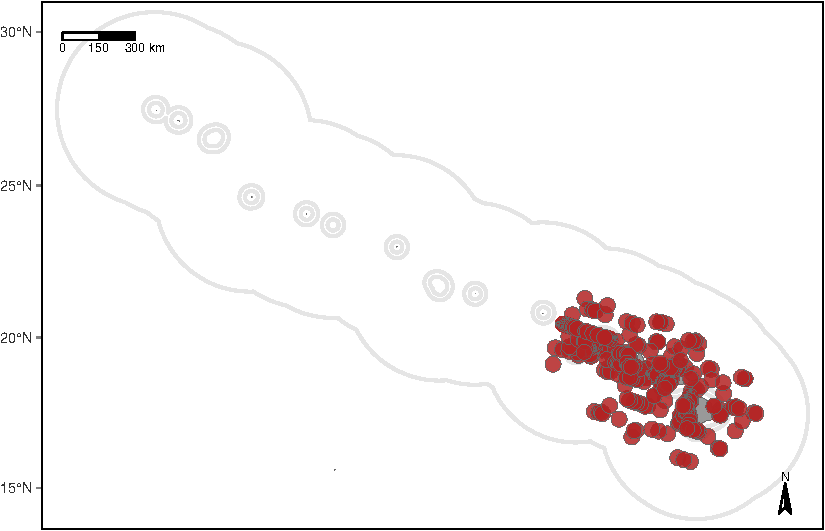
\includegraphics{figures/unnamed-chunk-77-1.pdf}

And the \texttt{das} slot holds the original \texttt{data.frame} of \texttt{DAS} data, modified slightly: the column \texttt{OnEffort} has been modified according to Beaufort range conditions, and the column \texttt{seg\_id} indicates which segment the event occurs within.

\begin{Shaded}
\begin{Highlighting}[]
\NormalTok{cruz}\SpecialCharTok{$}\NormalTok{cohorts}\SpecialCharTok{$}\NormalTok{all}\SpecialCharTok{$}\NormalTok{das }\SpecialCharTok{\%\textgreater{}\%}\NormalTok{ names}
\NormalTok{ [}\DecValTok{1}\NormalTok{] }\StringTok{"Event"}            \StringTok{"DateTime"}         \StringTok{"Lat"}              \StringTok{"Lon"}             
\NormalTok{ [}\DecValTok{5}\NormalTok{] }\StringTok{"OnEffort"}         \StringTok{"Cruise"}           \StringTok{"Mode"}             \StringTok{"OffsetGMT"}       
\NormalTok{ [}\DecValTok{9}\NormalTok{] }\StringTok{"EffType"}          \StringTok{"ESWsides"}         \StringTok{"Course"}           \StringTok{"SpdKt"}           
\NormalTok{[}\DecValTok{13}\NormalTok{] }\StringTok{"Bft"}              \StringTok{"SwellHght"}        \StringTok{"WindSpdKt"}        \StringTok{"RainFog"}         
\NormalTok{[}\DecValTok{17}\NormalTok{] }\StringTok{"HorizSun"}         \StringTok{"VertSun"}          \StringTok{"Glare"}            \StringTok{"Vis"}             
\NormalTok{[}\DecValTok{21}\NormalTok{] }\StringTok{"ObsL"}             \StringTok{"Rec"}              \StringTok{"ObsR"}             \StringTok{"ObsInd"}          
\NormalTok{[}\DecValTok{25}\NormalTok{] }\StringTok{"Data1"}            \StringTok{"Data2"}            \StringTok{"Data3"}            \StringTok{"Data4"}           
\NormalTok{[}\DecValTok{29}\NormalTok{] }\StringTok{"Data5"}            \StringTok{"Data6"}            \StringTok{"Data7"}            \StringTok{"Data8"}           
\NormalTok{[}\DecValTok{33}\NormalTok{] }\StringTok{"Data9"}            \StringTok{"Data10"}           \StringTok{"Data11"}           \StringTok{"Data12"}          
\NormalTok{[}\DecValTok{37}\NormalTok{] }\StringTok{"EffortDot"}        \StringTok{"EventNum"}         \StringTok{"file\_das"}         \StringTok{"line\_num"}        
\NormalTok{[}\DecValTok{41}\NormalTok{] }\StringTok{"stratum\_HI\_EEZ"}   \StringTok{"stratum\_OtherCNP"} \StringTok{"stratum\_WHICEAS"}  \StringTok{"year"}            
\NormalTok{[}\DecValTok{45}\NormalTok{] }\StringTok{"month"}            \StringTok{"day"}              \StringTok{"yday"}             \StringTok{"km\_int"}          
\NormalTok{[}\DecValTok{49}\NormalTok{] }\StringTok{"km\_cum"}           \StringTok{"ship"}             \StringTok{"stratum"}          \StringTok{"seg\_id"}          
\NormalTok{[}\DecValTok{53}\NormalTok{] }\StringTok{"use"}             
\end{Highlighting}
\end{Shaded}

The \texttt{segmentize()} function and its associated settings were designed to give researchers full control over how data are segmented, be it for design-based density analysis (which tend to use long segments of 100 km or more and allow for non-contiguous effort to be included in the same segment) or for habitat modeling (which tend to use short segments of 5 - 10 km and disallow non-contiguous effort to be pooled into the same segment). To demonstrate that versatility, checkout the \protect\hyperlink{segmentizing}{appendix on segmentizing}.

\hypertarget{process-sightings}{%
\subsection*{Process sightings}\label{process-sightings}}
\addcontentsline{toc}{subsection}{Process sightings}

To process sightings for each cohort of species, use the function \texttt{process\_sightings()}. This function has three basic steps: for each cohort, the function (1) prepares a sightings table using the function \texttt{das\_sight()} from \texttt{swfscDAS}; (2) filters those sightings to species codes specified for the cohort in your \texttt{settings} input; and (3) evaluates each of those sightings, asking if each should be included in the analysis according to your \texttt{settings}.

\begin{Shaded}
\begin{Highlighting}[]
\NormalTok{cruz }\OtherTok{\textless{}{-}} \FunctionTok{process\_sightings}\NormalTok{(cruz)}
\end{Highlighting}
\end{Shaded}

The function produces a formatted dataset and adds it to a new \texttt{sightings} slot.

\begin{Shaded}
\begin{Highlighting}[]
\NormalTok{cruz}\SpecialCharTok{$}\NormalTok{cohorts}\SpecialCharTok{$}\NormalTok{all }\SpecialCharTok{\%\textgreater{}\%}\NormalTok{ names}
\NormalTok{[}\DecValTok{1}\NormalTok{] }\StringTok{"segments"}  \StringTok{"das"}       \StringTok{"sightings"}

\NormalTok{cruz}\SpecialCharTok{$}\NormalTok{cohorts}\SpecialCharTok{$}\NormalTok{bottlenose }\SpecialCharTok{\%\textgreater{}\%}\NormalTok{ names}
\NormalTok{[}\DecValTok{1}\NormalTok{] }\StringTok{"segments"}  \StringTok{"das"}       \StringTok{"sightings"}

\NormalTok{cruz}\SpecialCharTok{$}\NormalTok{cohorts}\SpecialCharTok{$}\NormalTok{spotted }\SpecialCharTok{\%\textgreater{}\%}\NormalTok{ names}
\NormalTok{[}\DecValTok{1}\NormalTok{] }\StringTok{"segments"}  \StringTok{"das"}       \StringTok{"sightings"}
\end{Highlighting}
\end{Shaded}

Note that the \texttt{sightings} table has a column named \texttt{included} (\texttt{TRUE} = yes, use it in the analysis). Any sightings that do not meet the inclusion criteria as specified in your settings will be \texttt{included\ =\ FALSE}, but they won't be removed from the data.

The \texttt{sightings} table also has a new column, \texttt{ss\_valid},
indicating whether or not the group size estimate for this sighting
is valid and appropriate for use in abundance estimation and detection function fitting
when group size is used as a covariate.

Since the sightings in each cohort are processed slightly differently according to the cohort's specific settings -- most importantly the species that will be included -- you should expect different numbers of included/excluded sightings in each cohort dataset:

\begin{Shaded}
\begin{Highlighting}[]
\NormalTok{cruz}\SpecialCharTok{$}\NormalTok{cohorts}\SpecialCharTok{$}\NormalTok{all}\SpecialCharTok{$}\NormalTok{sightings}\SpecialCharTok{$}\NormalTok{included }\SpecialCharTok{\%\textgreater{}\%}\NormalTok{ table}
\NormalTok{.}
\ConstantTok{FALSE}  \ConstantTok{TRUE} 
  \DecValTok{810}  \DecValTok{3124} 

\NormalTok{cruz}\SpecialCharTok{$}\NormalTok{cohorts}\SpecialCharTok{$}\NormalTok{bottlenose}\SpecialCharTok{$}\NormalTok{sightings}\SpecialCharTok{$}\NormalTok{included }\SpecialCharTok{\%\textgreater{}\%}\NormalTok{ table}
\NormalTok{.}
\ConstantTok{FALSE}  \ConstantTok{TRUE} 
  \DecValTok{114}   \DecValTok{409} 
\end{Highlighting}
\end{Shaded}

When this function's \texttt{verbose} argument is \texttt{TRUE} (the default), a message is printed each time a sighting does not meet the inclusion criteria.

\hypertarget{sightings-data-structure}{%
\subsubsection*{Sightings data structure}\label{sightings-data-structure}}
\addcontentsline{toc}{subsubsection}{Sightings data structure}

The \texttt{sightings} table has many other variables:

\begin{Shaded}
\begin{Highlighting}[]
\NormalTok{cruz}\SpecialCharTok{$}\NormalTok{cohorts}\SpecialCharTok{$}\NormalTok{all}\SpecialCharTok{$}\NormalTok{sightings }\SpecialCharTok{\%\textgreater{}\%}\NormalTok{ names}
\NormalTok{ [}\DecValTok{1}\NormalTok{] }\StringTok{"Event"}            \StringTok{"DateTime"}         \StringTok{"Lat"}              \StringTok{"Lon"}             
\NormalTok{ [}\DecValTok{5}\NormalTok{] }\StringTok{"OnEffort"}         \StringTok{"Cruise"}           \StringTok{"Mode"}             \StringTok{"OffsetGMT"}       
\NormalTok{ [}\DecValTok{9}\NormalTok{] }\StringTok{"EffType"}          \StringTok{"ESWsides"}         \StringTok{"Course"}           \StringTok{"SpdKt"}           
\NormalTok{[}\DecValTok{13}\NormalTok{] }\StringTok{"Bft"}              \StringTok{"SwellHght"}        \StringTok{"WindSpdKt"}        \StringTok{"RainFog"}         
\NormalTok{[}\DecValTok{17}\NormalTok{] }\StringTok{"HorizSun"}         \StringTok{"VertSun"}          \StringTok{"Glare"}            \StringTok{"Vis"}             
\NormalTok{[}\DecValTok{21}\NormalTok{] }\StringTok{"ObsL"}             \StringTok{"Rec"}              \StringTok{"ObsR"}             \StringTok{"ObsInd"}          
\NormalTok{[}\DecValTok{25}\NormalTok{] }\StringTok{"EffortDot"}        \StringTok{"EventNum"}         \StringTok{"file\_das"}         \StringTok{"line\_num"}        
\NormalTok{[}\DecValTok{29}\NormalTok{] }\StringTok{"stratum\_HI\_EEZ"}   \StringTok{"stratum\_OtherCNP"} \StringTok{"stratum\_WHICEAS"}  \StringTok{"year"}            
\NormalTok{[}\DecValTok{33}\NormalTok{] }\StringTok{"month"}            \StringTok{"day"}              \StringTok{"yday"}             \StringTok{"km\_int"}          
\NormalTok{[}\DecValTok{37}\NormalTok{] }\StringTok{"km\_cum"}           \StringTok{"ship"}             \StringTok{"stratum"}          \StringTok{"seg\_id"}          
\NormalTok{[}\DecValTok{41}\NormalTok{] }\StringTok{"use"}              \StringTok{"SightNo"}          \StringTok{"Subgroup"}         \StringTok{"SightNoDaily"}    
\NormalTok{[}\DecValTok{45}\NormalTok{] }\StringTok{"Obs"}              \StringTok{"ObsStd"}           \StringTok{"Bearing"}          \StringTok{"Reticle"}         
\NormalTok{[}\DecValTok{49}\NormalTok{] }\StringTok{"DistNm"}           \StringTok{"Cue"}              \StringTok{"Method"}           \StringTok{"Photos"}          
\NormalTok{[}\DecValTok{53}\NormalTok{] }\StringTok{"Birds"}            \StringTok{"CalibSchool"}      \StringTok{"PhotosAerial"}     \StringTok{"Biopsy"}          
\NormalTok{[}\DecValTok{57}\NormalTok{] }\StringTok{"CourseSchool"}     \StringTok{"TurtleSp"}         \StringTok{"TurtleGs"}         \StringTok{"TurtleJFR"}       
\NormalTok{[}\DecValTok{61}\NormalTok{] }\StringTok{"TurtleAge"}        \StringTok{"TurtleCapt"}       \StringTok{"PinnipedSp"}       \StringTok{"PinnipedGs"}      
\NormalTok{[}\DecValTok{65}\NormalTok{] }\StringTok{"BoatType"}         \StringTok{"BoatGs"}           \StringTok{"PerpDistKm"}       \StringTok{"species"}         
\NormalTok{[}\DecValTok{69}\NormalTok{] }\StringTok{"best"}             \StringTok{"low"}              \StringTok{"high"}             \StringTok{"prob"}            
\NormalTok{[}\DecValTok{73}\NormalTok{] }\StringTok{"mixed"}            \StringTok{"ss\_tot"}           \StringTok{"lnsstot"}          \StringTok{"ss\_percent"}      
\NormalTok{[}\DecValTok{77}\NormalTok{] }\StringTok{"n\_sp"}             \StringTok{"n\_obs"}            \StringTok{"n\_best"}           \StringTok{"n\_low"}           
\NormalTok{[}\DecValTok{81}\NormalTok{] }\StringTok{"n\_high"}           \StringTok{"calibr"}           \StringTok{"ss\_valid"}         \StringTok{"mixed\_max"}       
\NormalTok{[}\DecValTok{85}\NormalTok{] }\StringTok{"spp\_max"}          \StringTok{"included"}        
\end{Highlighting}
\end{Shaded}

Columns 42 onwards correspond to sightings information. Columns of note:

\begin{itemize}
\item
  \texttt{species} contains the species code. There is only one species-code per row (i.e, multi-species sightings have been expanded to multiple rows).
\item
  \texttt{best}, \texttt{low}, and \texttt{high} contain the refined group size estimates, averaged across observers and calibrated according to the cohort's settings specifications. For multi-species sightings, these numbers represent the number of individuals for the single species represented in the row (i.e., the original group size estimate has been scaled by the percentage attritbuted to this species).
\item
  The columns following those group size estimates (\texttt{prob} through \texttt{spp\_max}) detail how group sizes were estimated: \texttt{prob} indicates whether probable species codes were accepted; \texttt{mixed} indicates whether this species' sighting is part of a mixed-species sighting; \texttt{n\_sp} provides the number of species occurring in this sighitng; \texttt{n\_obs} gives the number of observers who contributed group size estimates; \texttt{n\_best} through \texttt{n\_high} gives the number of valid group size estimates given; and \texttt{calibr} indicates whether or not calibration was attempted for this sighting based on the settings (see next section); \texttt{mixed\_max} indicates whether this species was the most abundant in the sighting (if multi-species); \texttt{spp\_max} indicates the species code for the most abundant species in the sighting (if multi-species).
\item
  As explained above, the final column, \texttt{included}, indicates whether this species should be included in the analysis.
\end{itemize}

Here is a glimpse of the data:

\begin{Shaded}
\begin{Highlighting}[]
\NormalTok{cruz}\SpecialCharTok{$}\NormalTok{cohorts}\SpecialCharTok{$}\NormalTok{all}\SpecialCharTok{$}\NormalTok{sightings }\SpecialCharTok{\%\textgreater{}\%}\NormalTok{ glimpse}
\NormalTok{Rows}\SpecialCharTok{:} \DecValTok{3}\NormalTok{,}\DecValTok{934}
\NormalTok{Columns}\SpecialCharTok{:} \DecValTok{86}
\SpecialCharTok{$}\NormalTok{ Event            }\SpecialCharTok{\textless{}}\NormalTok{chr}\SpecialCharTok{\textgreater{}} \StringTok{"S"}\NormalTok{, }\StringTok{"S"}\NormalTok{, }\StringTok{"S"}\NormalTok{, }\StringTok{"S"}\NormalTok{, }\StringTok{"S"}\NormalTok{, }\StringTok{"S"}\NormalTok{, }\StringTok{"S"}\NormalTok{, }\StringTok{"S"}\NormalTok{, }\StringTok{"S"}\NormalTok{, }\StringTok{"S"}\NormalTok{, }\StringTok{"S"}\SpecialCharTok{\textasciitilde{}}
\ErrorTok{$}\NormalTok{ DateTime         }\SpecialCharTok{\textless{}}\NormalTok{dttm}\SpecialCharTok{\textgreater{}} \DecValTok{1986{-}11{-}26} \DecValTok{09}\SpecialCharTok{:}\DecValTok{00}\SpecialCharTok{:}\DecValTok{00}\NormalTok{, }\DecValTok{1986{-}11{-}26} \DecValTok{14}\SpecialCharTok{:}\DecValTok{40}\SpecialCharTok{:}\DecValTok{00}\NormalTok{, }\DecValTok{1986{-}11{-}26}\SpecialCharTok{\textasciitilde{}}
\ErrorTok{$}\NormalTok{ Lat              }\SpecialCharTok{\textless{}}\NormalTok{dbl}\SpecialCharTok{\textgreater{}} \FloatTok{4.983333}\NormalTok{, }\FloatTok{5.616667}\NormalTok{, }\FloatTok{5.866667}\NormalTok{, }\FloatTok{7.050000}\NormalTok{, }\FloatTok{7.466667}\NormalTok{, }\FloatTok{9.4}\SpecialCharTok{\textasciitilde{}}
\ErrorTok{$}\NormalTok{ Lon              }\SpecialCharTok{\textless{}}\NormalTok{dbl}\SpecialCharTok{\textgreater{}} \SpecialCharTok{{-}}\FloatTok{120.9500}\NormalTok{, }\SpecialCharTok{{-}}\FloatTok{121.6667}\NormalTok{, }\SpecialCharTok{{-}}\FloatTok{121.9833}\NormalTok{, }\SpecialCharTok{{-}}\FloatTok{123.5000}\NormalTok{, }\SpecialCharTok{{-}}\FloatTok{123.9167}\SpecialCharTok{\textasciitilde{}}
\ErrorTok{$}\NormalTok{ OnEffort         }\SpecialCharTok{\textless{}}\NormalTok{lgl}\SpecialCharTok{\textgreater{}} \ConstantTok{TRUE}\NormalTok{, }\ConstantTok{TRUE}\NormalTok{, }\ConstantTok{TRUE}\NormalTok{, }\ConstantTok{TRUE}\NormalTok{, }\ConstantTok{TRUE}\NormalTok{, }\ConstantTok{TRUE}\NormalTok{, }\ConstantTok{TRUE}\NormalTok{, }\ConstantTok{TRUE}\NormalTok{, }\ConstantTok{TRUE}\NormalTok{,}\SpecialCharTok{\textasciitilde{}}
\ErrorTok{$}\NormalTok{ Cruise           }\SpecialCharTok{\textless{}}\NormalTok{dbl}\SpecialCharTok{\textgreater{}} \DecValTok{989}\NormalTok{, }\DecValTok{989}\NormalTok{, }\DecValTok{989}\NormalTok{, }\DecValTok{989}\NormalTok{, }\DecValTok{989}\NormalTok{, }\DecValTok{989}\NormalTok{, }\DecValTok{989}\NormalTok{, }\DecValTok{989}\NormalTok{, }\DecValTok{989}\NormalTok{, }\DecValTok{989}\NormalTok{, }\DecValTok{989}\SpecialCharTok{\textasciitilde{}}
\ErrorTok{$}\NormalTok{ Mode             }\SpecialCharTok{\textless{}}\NormalTok{chr}\SpecialCharTok{\textgreater{}} \StringTok{"C"}\NormalTok{, }\StringTok{"C"}\NormalTok{, }\StringTok{"C"}\NormalTok{, }\StringTok{"C"}\NormalTok{, }\StringTok{"C"}\NormalTok{, }\StringTok{"C"}\NormalTok{, }\StringTok{"C"}\NormalTok{, }\StringTok{"C"}\NormalTok{, }\StringTok{"C"}\NormalTok{, }\StringTok{"C"}\NormalTok{, }\StringTok{"C"}\SpecialCharTok{\textasciitilde{}}
\ErrorTok{$}\NormalTok{ OffsetGMT        }\SpecialCharTok{\textless{}}\NormalTok{int}\SpecialCharTok{\textgreater{}} \ConstantTok{NA}\NormalTok{, }\ConstantTok{NA}\NormalTok{, }\ConstantTok{NA}\NormalTok{, }\ConstantTok{NA}\NormalTok{, }\ConstantTok{NA}\NormalTok{, }\ConstantTok{NA}\NormalTok{, }\ConstantTok{NA}\NormalTok{, }\ConstantTok{NA}\NormalTok{, }\ConstantTok{NA}\NormalTok{, }\ConstantTok{NA}\NormalTok{, }\ConstantTok{NA}\NormalTok{, }\ConstantTok{NA}\NormalTok{, }\ConstantTok{NA}\NormalTok{, N}\SpecialCharTok{\textasciitilde{}}
\ErrorTok{$}\NormalTok{ EffType          }\SpecialCharTok{\textless{}}\NormalTok{chr}\SpecialCharTok{\textgreater{}} \StringTok{"S"}\NormalTok{, }\StringTok{"S"}\NormalTok{, }\StringTok{"S"}\NormalTok{, }\StringTok{"S"}\NormalTok{, }\StringTok{"S"}\NormalTok{, }\StringTok{"S"}\NormalTok{, }\StringTok{"S"}\NormalTok{, }\StringTok{"S"}\NormalTok{, }\StringTok{"S"}\NormalTok{, }\StringTok{"S"}\NormalTok{, }\StringTok{"S"}\SpecialCharTok{\textasciitilde{}}
\ErrorTok{$}\NormalTok{ ESWsides         }\SpecialCharTok{\textless{}}\NormalTok{dbl}\SpecialCharTok{\textgreater{}} \DecValTok{2}\NormalTok{, }\DecValTok{2}\NormalTok{, }\DecValTok{2}\NormalTok{, }\DecValTok{2}\NormalTok{, }\DecValTok{2}\NormalTok{, }\DecValTok{2}\NormalTok{, }\DecValTok{2}\NormalTok{, }\DecValTok{2}\NormalTok{, }\DecValTok{2}\NormalTok{, }\DecValTok{2}\NormalTok{, }\DecValTok{2}\NormalTok{, }\DecValTok{2}\NormalTok{, }\DecValTok{2}\NormalTok{, }\DecValTok{2}\NormalTok{, }\DecValTok{2}\NormalTok{, }\DecValTok{2}\NormalTok{, }\DecValTok{2}\NormalTok{, }\DecValTok{2}\NormalTok{,}\SpecialCharTok{\textasciitilde{}}
\ErrorTok{$}\NormalTok{ Course           }\SpecialCharTok{\textless{}}\NormalTok{dbl}\SpecialCharTok{\textgreater{}} \DecValTok{310}\NormalTok{, }\DecValTok{316}\NormalTok{, }\DecValTok{313}\NormalTok{, }\DecValTok{310}\NormalTok{, }\DecValTok{310}\NormalTok{, }\DecValTok{305}\NormalTok{, }\DecValTok{305}\NormalTok{, }\DecValTok{305}\NormalTok{, }\DecValTok{305}\NormalTok{, }\DecValTok{305}\NormalTok{, }\DecValTok{305}\SpecialCharTok{\textasciitilde{}}
\ErrorTok{$}\NormalTok{ SpdKt            }\SpecialCharTok{\textless{}}\NormalTok{dbl}\SpecialCharTok{\textgreater{}} \FloatTok{10.2}\NormalTok{, }\FloatTok{9.9}\NormalTok{, }\FloatTok{9.6}\NormalTok{, }\FloatTok{10.2}\NormalTok{, }\FloatTok{10.3}\NormalTok{, }\FloatTok{9.8}\NormalTok{, }\FloatTok{9.8}\NormalTok{, }\FloatTok{9.6}\NormalTok{, }\FloatTok{10.1}\NormalTok{, }\FloatTok{10.1}\SpecialCharTok{\textasciitilde{}}
\ErrorTok{$}\NormalTok{ Bft              }\SpecialCharTok{\textless{}}\NormalTok{dbl}\SpecialCharTok{\textgreater{}} \DecValTok{4}\NormalTok{, }\DecValTok{4}\NormalTok{, }\DecValTok{4}\NormalTok{, }\DecValTok{3}\NormalTok{, }\DecValTok{3}\NormalTok{, }\DecValTok{2}\NormalTok{, }\DecValTok{2}\NormalTok{, }\DecValTok{2}\NormalTok{, }\DecValTok{1}\NormalTok{, }\DecValTok{1}\NormalTok{, }\DecValTok{1}\NormalTok{, }\DecValTok{4}\NormalTok{, }\DecValTok{5}\NormalTok{, }\DecValTok{4}\NormalTok{, }\DecValTok{4}\NormalTok{, }\DecValTok{3}\NormalTok{, }\DecValTok{1}\NormalTok{, }\DecValTok{2}\NormalTok{,}\SpecialCharTok{\textasciitilde{}}
\ErrorTok{$}\NormalTok{ SwellHght        }\SpecialCharTok{\textless{}}\NormalTok{dbl}\SpecialCharTok{\textgreater{}} \ConstantTok{NA}\NormalTok{, }\ConstantTok{NA}\NormalTok{, }\ConstantTok{NA}\NormalTok{, }\ConstantTok{NA}\NormalTok{, }\ConstantTok{NA}\NormalTok{, }\ConstantTok{NA}\NormalTok{, }\ConstantTok{NA}\NormalTok{, }\ConstantTok{NA}\NormalTok{, }\ConstantTok{NA}\NormalTok{, }\ConstantTok{NA}\NormalTok{, }\ConstantTok{NA}\NormalTok{, }\ConstantTok{NA}\NormalTok{, }\ConstantTok{NA}\NormalTok{, N}\SpecialCharTok{\textasciitilde{}}
\ErrorTok{$}\NormalTok{ WindSpdKt        }\SpecialCharTok{\textless{}}\NormalTok{dbl}\SpecialCharTok{\textgreater{}} \ConstantTok{NA}\NormalTok{, }\ConstantTok{NA}\NormalTok{, }\ConstantTok{NA}\NormalTok{, }\ConstantTok{NA}\NormalTok{, }\ConstantTok{NA}\NormalTok{, }\ConstantTok{NA}\NormalTok{, }\ConstantTok{NA}\NormalTok{, }\ConstantTok{NA}\NormalTok{, }\ConstantTok{NA}\NormalTok{, }\ConstantTok{NA}\NormalTok{, }\ConstantTok{NA}\NormalTok{, }\ConstantTok{NA}\NormalTok{, }\ConstantTok{NA}\NormalTok{, N}\SpecialCharTok{\textasciitilde{}}
\ErrorTok{$}\NormalTok{ RainFog          }\SpecialCharTok{\textless{}}\NormalTok{dbl}\SpecialCharTok{\textgreater{}} \DecValTok{1}\NormalTok{, }\DecValTok{1}\NormalTok{, }\DecValTok{1}\NormalTok{, }\DecValTok{1}\NormalTok{, }\DecValTok{1}\NormalTok{, }\DecValTok{1}\NormalTok{, }\DecValTok{1}\NormalTok{, }\DecValTok{1}\NormalTok{, }\DecValTok{1}\NormalTok{, }\DecValTok{1}\NormalTok{, }\DecValTok{1}\NormalTok{, }\DecValTok{1}\NormalTok{, }\DecValTok{1}\NormalTok{, }\DecValTok{1}\NormalTok{, }\DecValTok{1}\NormalTok{, }\DecValTok{1}\NormalTok{, }\DecValTok{1}\NormalTok{, }\DecValTok{1}\NormalTok{,}\SpecialCharTok{\textasciitilde{}}
\ErrorTok{$}\NormalTok{ HorizSun         }\SpecialCharTok{\textless{}}\NormalTok{dbl}\SpecialCharTok{\textgreater{}} \DecValTok{6}\NormalTok{, }\DecValTok{9}\NormalTok{, }\DecValTok{10}\NormalTok{, }\ConstantTok{NA}\NormalTok{, }\DecValTok{7}\NormalTok{, }\DecValTok{5}\NormalTok{, }\DecValTok{5}\NormalTok{, }\DecValTok{7}\NormalTok{, }\DecValTok{8}\NormalTok{, }\DecValTok{8}\NormalTok{, }\DecValTok{8}\NormalTok{, }\DecValTok{3}\NormalTok{, }\DecValTok{5}\NormalTok{, }\ConstantTok{NA}\NormalTok{, }\DecValTok{4}\NormalTok{, }\ConstantTok{NA}\NormalTok{, N}\SpecialCharTok{\textasciitilde{}}
\ErrorTok{$}\NormalTok{ VertSun          }\SpecialCharTok{\textless{}}\NormalTok{dbl}\SpecialCharTok{\textgreater{}} \DecValTok{2}\NormalTok{, }\DecValTok{1}\NormalTok{, }\DecValTok{3}\NormalTok{, }\ConstantTok{NA}\NormalTok{, }\DecValTok{1}\NormalTok{, }\DecValTok{3}\NormalTok{, }\DecValTok{3}\NormalTok{, }\DecValTok{1}\NormalTok{, }\DecValTok{1}\NormalTok{, }\DecValTok{1}\NormalTok{, }\DecValTok{1}\NormalTok{, }\DecValTok{2}\NormalTok{, }\DecValTok{1}\NormalTok{, }\ConstantTok{NA}\NormalTok{, }\DecValTok{1}\NormalTok{, }\ConstantTok{NA}\NormalTok{, }\ConstantTok{NA}\SpecialCharTok{\textasciitilde{}}
\ErrorTok{$}\NormalTok{ Glare            }\SpecialCharTok{\textless{}}\NormalTok{lgl}\SpecialCharTok{\textgreater{}} \ConstantTok{FALSE}\NormalTok{, }\ConstantTok{FALSE}\NormalTok{, }\ConstantTok{FALSE}\NormalTok{, }\ConstantTok{NA}\NormalTok{, }\ConstantTok{FALSE}\NormalTok{, }\ConstantTok{FALSE}\NormalTok{, }\ConstantTok{FALSE}\NormalTok{, }\ConstantTok{FALSE}\NormalTok{, }\SpecialCharTok{\textasciitilde{}}
\ErrorTok{$}\NormalTok{ Vis              }\SpecialCharTok{\textless{}}\NormalTok{dbl}\SpecialCharTok{\textgreater{}} \ConstantTok{NA}\NormalTok{, }\ConstantTok{NA}\NormalTok{, }\ConstantTok{NA}\NormalTok{, }\ConstantTok{NA}\NormalTok{, }\ConstantTok{NA}\NormalTok{, }\ConstantTok{NA}\NormalTok{, }\ConstantTok{NA}\NormalTok{, }\ConstantTok{NA}\NormalTok{, }\ConstantTok{NA}\NormalTok{, }\ConstantTok{NA}\NormalTok{, }\ConstantTok{NA}\NormalTok{, }\ConstantTok{NA}\NormalTok{, }\ConstantTok{NA}\NormalTok{, N}\SpecialCharTok{\textasciitilde{}}
\ErrorTok{$}\NormalTok{ ObsL             }\SpecialCharTok{\textless{}}\NormalTok{chr}\SpecialCharTok{\textgreater{}} \StringTok{"004"}\NormalTok{, }\StringTok{"022"}\NormalTok{, }\StringTok{"056"}\NormalTok{, }\StringTok{"056"}\NormalTok{, }\StringTok{"004"}\NormalTok{, }\StringTok{"031"}\NormalTok{, }\StringTok{"031"}\NormalTok{, }\StringTok{"004\textasciitilde{}}
\StringTok{$ Rec              \textless{}chr\textgreater{} "}\DecValTok{056}\StringTok{", "}\DecValTok{031}\StringTok{", "}\DecValTok{062}\StringTok{", "}\DecValTok{062}\StringTok{", "}\DecValTok{056}\StringTok{", "}\DecValTok{022}\StringTok{", "}\DecValTok{022}\StringTok{", "}\DecValTok{056}\SpecialCharTok{\textasciitilde{}}
\ErrorTok{$}\NormalTok{ ObsR             }\SpecialCharTok{\textless{}}\NormalTok{chr}\SpecialCharTok{\textgreater{}} \StringTok{"062"}\NormalTok{, }\StringTok{"057"}\NormalTok{, }\StringTok{"004"}\NormalTok{, }\StringTok{"004"}\NormalTok{, }\StringTok{"062"}\NormalTok{, }\StringTok{"057"}\NormalTok{, }\StringTok{"057"}\NormalTok{, }\StringTok{"062\textasciitilde{}}
\StringTok{$ ObsInd           \textless{}chr\textgreater{} NA, NA, NA, NA, NA, NA, NA, NA, NA, NA, NA, NA, NA, N\textasciitilde{}}
\StringTok{$ EffortDot        \textless{}lgl\textgreater{} TRUE, TRUE, TRUE, TRUE, TRUE, TRUE, TRUE, TRUE, TRUE,\textasciitilde{}}
\StringTok{$ EventNum         \textless{}chr\textgreater{} "}\DecValTok{18}\StringTok{", "}\DecValTok{43}\StringTok{", "}\DecValTok{59}\StringTok{", "}\DecValTok{9}\StringTok{", "}\DecValTok{32}\StringTok{", "}\DecValTok{10}\StringTok{", "}\DecValTok{10}\StringTok{", "}\DecValTok{22}\StringTok{", "}\DecValTok{34}\StringTok{", \textasciitilde{}}
\StringTok{$ file\_das         \textless{}chr\textgreater{} "}\NormalTok{CenPac1986}\SpecialCharTok{{-}}\NormalTok{2020\_Final\_alb.das}\StringTok{", "}\NormalTok{CenPac1986}\SpecialCharTok{{-}}\NormalTok{2020\_Fin}\SpecialCharTok{\textasciitilde{}}
\ErrorTok{$}\NormalTok{ line\_num         }\SpecialCharTok{\textless{}}\NormalTok{int}\SpecialCharTok{\textgreater{}} \DecValTok{10295}\NormalTok{, }\DecValTok{10321}\NormalTok{, }\DecValTok{10340}\NormalTok{, }\DecValTok{10358}\NormalTok{, }\DecValTok{10384}\NormalTok{, }\DecValTok{10451}\NormalTok{, }\DecValTok{10451}\NormalTok{, }\DecValTok{1046}\SpecialCharTok{\textasciitilde{}}
\ErrorTok{$}\NormalTok{ stratum\_HI\_EEZ   }\SpecialCharTok{\textless{}}\NormalTok{lgl}\SpecialCharTok{\textgreater{}} \ConstantTok{FALSE}\NormalTok{, }\ConstantTok{FALSE}\NormalTok{, }\ConstantTok{FALSE}\NormalTok{, }\ConstantTok{FALSE}\NormalTok{, }\ConstantTok{FALSE}\NormalTok{, }\ConstantTok{FALSE}\NormalTok{, }\ConstantTok{FALSE}\NormalTok{, FALS}\SpecialCharTok{\textasciitilde{}}
\ErrorTok{$}\NormalTok{ stratum\_OtherCNP }\SpecialCharTok{\textless{}}\NormalTok{lgl}\SpecialCharTok{\textgreater{}} \ConstantTok{TRUE}\NormalTok{, }\ConstantTok{TRUE}\NormalTok{, }\ConstantTok{TRUE}\NormalTok{, }\ConstantTok{TRUE}\NormalTok{, }\ConstantTok{TRUE}\NormalTok{, }\ConstantTok{TRUE}\NormalTok{, }\ConstantTok{TRUE}\NormalTok{, }\ConstantTok{TRUE}\NormalTok{, }\ConstantTok{TRUE}\NormalTok{,}\SpecialCharTok{\textasciitilde{}}
\ErrorTok{$}\NormalTok{ stratum\_WHICEAS  }\SpecialCharTok{\textless{}}\NormalTok{lgl}\SpecialCharTok{\textgreater{}} \ConstantTok{FALSE}\NormalTok{, }\ConstantTok{FALSE}\NormalTok{, }\ConstantTok{FALSE}\NormalTok{, }\ConstantTok{FALSE}\NormalTok{, }\ConstantTok{FALSE}\NormalTok{, }\ConstantTok{FALSE}\NormalTok{, }\ConstantTok{FALSE}\NormalTok{, FALS}\SpecialCharTok{\textasciitilde{}}
\ErrorTok{$}\NormalTok{ year             }\SpecialCharTok{\textless{}}\NormalTok{dbl}\SpecialCharTok{\textgreater{}} \DecValTok{1986}\NormalTok{, }\DecValTok{1986}\NormalTok{, }\DecValTok{1986}\NormalTok{, }\DecValTok{1986}\NormalTok{, }\DecValTok{1986}\NormalTok{, }\DecValTok{1986}\NormalTok{, }\DecValTok{1986}\NormalTok{, }\DecValTok{1986}\NormalTok{, }\DecValTok{1986}\NormalTok{,}\SpecialCharTok{\textasciitilde{}}
\ErrorTok{$}\NormalTok{ month            }\SpecialCharTok{\textless{}}\NormalTok{dbl}\SpecialCharTok{\textgreater{}} \DecValTok{11}\NormalTok{, }\DecValTok{11}\NormalTok{, }\DecValTok{11}\NormalTok{, }\DecValTok{11}\NormalTok{, }\DecValTok{11}\NormalTok{, }\DecValTok{11}\NormalTok{, }\DecValTok{11}\NormalTok{, }\DecValTok{11}\NormalTok{, }\DecValTok{11}\NormalTok{, }\DecValTok{11}\NormalTok{, }\DecValTok{11}\NormalTok{, }\DecValTok{11}\NormalTok{, }\DecValTok{11}\NormalTok{, }\DecValTok{1}\SpecialCharTok{\textasciitilde{}}
\ErrorTok{$}\NormalTok{ day              }\SpecialCharTok{\textless{}}\NormalTok{int}\SpecialCharTok{\textgreater{}} \DecValTok{26}\NormalTok{, }\DecValTok{26}\NormalTok{, }\DecValTok{26}\NormalTok{, }\DecValTok{27}\NormalTok{, }\DecValTok{27}\NormalTok{, }\DecValTok{28}\NormalTok{, }\DecValTok{28}\NormalTok{, }\DecValTok{28}\NormalTok{, }\DecValTok{28}\NormalTok{, }\DecValTok{28}\NormalTok{, }\DecValTok{28}\NormalTok{, }\DecValTok{29}\NormalTok{, }\DecValTok{29}\NormalTok{, }\DecValTok{3}\SpecialCharTok{\textasciitilde{}}
\ErrorTok{$}\NormalTok{ yday             }\SpecialCharTok{\textless{}}\NormalTok{dbl}\SpecialCharTok{\textgreater{}} \DecValTok{330}\NormalTok{, }\DecValTok{330}\NormalTok{, }\DecValTok{330}\NormalTok{, }\DecValTok{331}\NormalTok{, }\DecValTok{331}\NormalTok{, }\DecValTok{332}\NormalTok{, }\DecValTok{332}\NormalTok{, }\DecValTok{332}\NormalTok{, }\DecValTok{332}\NormalTok{, }\DecValTok{332}\NormalTok{, }\DecValTok{332}\SpecialCharTok{\textasciitilde{}}
\ErrorTok{$}\NormalTok{ km\_int           }\SpecialCharTok{\textless{}}\NormalTok{dbl}\SpecialCharTok{\textgreater{}} \DecValTok{0}\NormalTok{, }\DecValTok{0}\NormalTok{, }\DecValTok{0}\NormalTok{, }\DecValTok{0}\NormalTok{, }\DecValTok{0}\NormalTok{, }\DecValTok{0}\NormalTok{, }\DecValTok{0}\NormalTok{, }\DecValTok{0}\NormalTok{, }\DecValTok{0}\NormalTok{, }\DecValTok{0}\NormalTok{, }\DecValTok{0}\NormalTok{, }\DecValTok{0}\NormalTok{, }\DecValTok{0}\NormalTok{, }\DecValTok{0}\NormalTok{, }\DecValTok{0}\NormalTok{, }\DecValTok{0}\NormalTok{, }\DecValTok{0}\NormalTok{, }\DecValTok{0}\NormalTok{,}\SpecialCharTok{\textasciitilde{}}
\ErrorTok{$}\NormalTok{ km\_cum           }\SpecialCharTok{\textless{}}\NormalTok{dbl}\SpecialCharTok{\textgreater{}} \FloatTok{64.38787}\NormalTok{, }\FloatTok{172.92124}\NormalTok{, }\FloatTok{221.24918}\NormalTok{, }\FloatTok{248.23899}\NormalTok{, }\FloatTok{317.83407}\NormalTok{,}\SpecialCharTok{\textasciitilde{}}
\ErrorTok{$}\NormalTok{ ship             }\SpecialCharTok{\textless{}}\NormalTok{chr}\SpecialCharTok{\textgreater{}} \StringTok{"DSJ"}\NormalTok{, }\StringTok{"DSJ"}\NormalTok{, }\StringTok{"DSJ"}\NormalTok{, }\StringTok{"DSJ"}\NormalTok{, }\StringTok{"DSJ"}\NormalTok{, }\StringTok{"DSJ"}\NormalTok{, }\StringTok{"DSJ"}\NormalTok{, }\StringTok{"DSJ\textasciitilde{}}
\StringTok{$ stratum          \textless{}chr\textgreater{} "}\NormalTok{OtherCNP}\StringTok{", "}\NormalTok{OtherCNP}\StringTok{", "}\NormalTok{OtherCNP}\StringTok{", "}\NormalTok{OtherCNP}\StringTok{", "}\NormalTok{Othe}\SpecialCharTok{\textasciitilde{}}
\ErrorTok{$}\NormalTok{ seg\_id           }\SpecialCharTok{\textless{}}\NormalTok{int}\SpecialCharTok{\textgreater{}} \DecValTok{34}\NormalTok{, }\DecValTok{35}\NormalTok{, }\DecValTok{35}\NormalTok{, }\DecValTok{35}\NormalTok{, }\DecValTok{36}\NormalTok{, }\DecValTok{37}\NormalTok{, }\DecValTok{37}\NormalTok{, }\DecValTok{37}\NormalTok{, }\DecValTok{37}\NormalTok{, }\DecValTok{37}\NormalTok{, }\DecValTok{29}\NormalTok{, }\DecValTok{38}\NormalTok{, }\DecValTok{38}\NormalTok{, }\DecValTok{3}\SpecialCharTok{\textasciitilde{}}
\ErrorTok{$}\NormalTok{ use              }\SpecialCharTok{\textless{}}\NormalTok{lgl}\SpecialCharTok{\textgreater{}} \ConstantTok{TRUE}\NormalTok{, }\ConstantTok{TRUE}\NormalTok{, }\ConstantTok{TRUE}\NormalTok{, }\ConstantTok{TRUE}\NormalTok{, }\ConstantTok{TRUE}\NormalTok{, }\ConstantTok{TRUE}\NormalTok{, }\ConstantTok{TRUE}\NormalTok{, }\ConstantTok{TRUE}\NormalTok{, }\ConstantTok{TRUE}\NormalTok{,}\SpecialCharTok{\textasciitilde{}}
\ErrorTok{$}\NormalTok{ SightNo          }\SpecialCharTok{\textless{}}\NormalTok{chr}\SpecialCharTok{\textgreater{}} \StringTok{"01"}\NormalTok{, }\StringTok{"02"}\NormalTok{, }\StringTok{"03"}\NormalTok{, }\StringTok{"01"}\NormalTok{, }\StringTok{"02"}\NormalTok{, }\StringTok{"01"}\NormalTok{, }\StringTok{"01"}\NormalTok{, }\StringTok{"02"}\NormalTok{, }\StringTok{"03"}\NormalTok{,}\SpecialCharTok{\textasciitilde{}}
\ErrorTok{$}\NormalTok{ Subgroup         }\SpecialCharTok{\textless{}}\NormalTok{chr}\SpecialCharTok{\textgreater{}} \ConstantTok{NA}\NormalTok{, }\ConstantTok{NA}\NormalTok{, }\ConstantTok{NA}\NormalTok{, }\ConstantTok{NA}\NormalTok{, }\ConstantTok{NA}\NormalTok{, }\ConstantTok{NA}\NormalTok{, }\ConstantTok{NA}\NormalTok{, }\ConstantTok{NA}\NormalTok{, }\ConstantTok{NA}\NormalTok{, }\ConstantTok{NA}\NormalTok{, }\ConstantTok{NA}\NormalTok{, }\ConstantTok{NA}\NormalTok{, }\ConstantTok{NA}\NormalTok{, N}\SpecialCharTok{\textasciitilde{}}
\ErrorTok{$}\NormalTok{ SightNoDaily     }\SpecialCharTok{\textless{}}\NormalTok{chr}\SpecialCharTok{\textgreater{}} \StringTok{"19861126\_1"}\NormalTok{, }\StringTok{"19861126\_2"}\NormalTok{, }\StringTok{"19861126\_3"}\NormalTok{, }\StringTok{"19861127\_1\textasciitilde{}}
\StringTok{$ Obs              \textless{}chr\textgreater{} "}\DecValTok{004}\StringTok{", "}\DecValTok{057}\StringTok{", "}\DecValTok{004}\StringTok{", "}\DecValTok{056}\StringTok{", "}\DecValTok{004}\StringTok{", "}\DecValTok{031}\StringTok{", "}\DecValTok{031}\StringTok{", "}\DecValTok{004}\SpecialCharTok{\textasciitilde{}}
\ErrorTok{$}\NormalTok{ ObsStd           }\SpecialCharTok{\textless{}}\NormalTok{lgl}\SpecialCharTok{\textgreater{}} \ConstantTok{TRUE}\NormalTok{, }\ConstantTok{TRUE}\NormalTok{, }\ConstantTok{TRUE}\NormalTok{, }\ConstantTok{TRUE}\NormalTok{, }\ConstantTok{TRUE}\NormalTok{, }\ConstantTok{TRUE}\NormalTok{, }\ConstantTok{TRUE}\NormalTok{, }\ConstantTok{TRUE}\NormalTok{, }\ConstantTok{TRUE}\NormalTok{,}\SpecialCharTok{\textasciitilde{}}
\ErrorTok{$}\NormalTok{ Bearing          }\SpecialCharTok{\textless{}}\NormalTok{dbl}\SpecialCharTok{\textgreater{}} \DecValTok{335}\NormalTok{, }\DecValTok{354}\NormalTok{, }\DecValTok{336}\NormalTok{, }\DecValTok{18}\NormalTok{, }\DecValTok{332}\NormalTok{, }\DecValTok{333}\NormalTok{, }\DecValTok{333}\NormalTok{, }\DecValTok{6}\NormalTok{, }\DecValTok{312}\NormalTok{, }\DecValTok{312}\NormalTok{, }\DecValTok{38}\NormalTok{, }\DecValTok{80}\SpecialCharTok{\textasciitilde{}}
\ErrorTok{$}\NormalTok{ Reticle          }\SpecialCharTok{\textless{}}\NormalTok{dbl}\SpecialCharTok{\textgreater{}} \FloatTok{8.41}\NormalTok{, }\FloatTok{3.88}\NormalTok{, }\FloatTok{0.50}\NormalTok{, }\FloatTok{11.40}\NormalTok{, }\FloatTok{0.80}\NormalTok{, }\FloatTok{0.30}\NormalTok{, }\FloatTok{0.30}\NormalTok{, }\FloatTok{2.98}\NormalTok{, }\FloatTok{0.40}\SpecialCharTok{\textasciitilde{}}
\ErrorTok{$}\NormalTok{ DistNm           }\SpecialCharTok{\textless{}}\NormalTok{dbl}\SpecialCharTok{\textgreater{}} \FloatTok{0.4}\NormalTok{, }\FloatTok{0.8}\NormalTok{, }\FloatTok{3.2}\NormalTok{, }\FloatTok{0.3}\NormalTok{, }\FloatTok{2.5}\NormalTok{, }\FloatTok{3.8}\NormalTok{, }\FloatTok{3.8}\NormalTok{, }\FloatTok{1.0}\NormalTok{, }\FloatTok{3.5}\NormalTok{, }\FloatTok{3.5}\NormalTok{, }\FloatTok{7.0}\SpecialCharTok{\textasciitilde{}}
\ErrorTok{$}\NormalTok{ Cue              }\SpecialCharTok{\textless{}}\NormalTok{dbl}\SpecialCharTok{\textgreater{}} \DecValTok{3}\NormalTok{, }\DecValTok{3}\NormalTok{, }\DecValTok{2}\NormalTok{, }\DecValTok{2}\NormalTok{, }\DecValTok{3}\NormalTok{, }\DecValTok{3}\NormalTok{, }\DecValTok{3}\NormalTok{, }\DecValTok{3}\NormalTok{, }\DecValTok{2}\NormalTok{, }\DecValTok{2}\NormalTok{, }\DecValTok{3}\NormalTok{, }\DecValTok{3}\NormalTok{, }\DecValTok{6}\NormalTok{, }\DecValTok{6}\NormalTok{, }\DecValTok{3}\NormalTok{, }\DecValTok{2}\NormalTok{, }\DecValTok{3}\NormalTok{, }\DecValTok{2}\NormalTok{,}\SpecialCharTok{\textasciitilde{}}
\ErrorTok{$}\NormalTok{ Method           }\SpecialCharTok{\textless{}}\NormalTok{dbl}\SpecialCharTok{\textgreater{}} \DecValTok{4}\NormalTok{, }\DecValTok{4}\NormalTok{, }\DecValTok{4}\NormalTok{, }\DecValTok{4}\NormalTok{, }\DecValTok{4}\NormalTok{, }\DecValTok{4}\NormalTok{, }\DecValTok{4}\NormalTok{, }\DecValTok{4}\NormalTok{, }\DecValTok{4}\NormalTok{, }\DecValTok{4}\NormalTok{, }\DecValTok{4}\NormalTok{, }\DecValTok{4}\NormalTok{, }\DecValTok{4}\NormalTok{, }\DecValTok{4}\NormalTok{, }\DecValTok{4}\NormalTok{, }\DecValTok{4}\NormalTok{, }\DecValTok{4}\NormalTok{, }\DecValTok{4}\NormalTok{,}\SpecialCharTok{\textasciitilde{}}
\ErrorTok{$}\NormalTok{ Photos           }\SpecialCharTok{\textless{}}\NormalTok{chr}\SpecialCharTok{\textgreater{}} \ConstantTok{NA}\NormalTok{, }\ConstantTok{NA}\NormalTok{, }\ConstantTok{NA}\NormalTok{, }\ConstantTok{NA}\NormalTok{, }\ConstantTok{NA}\NormalTok{, }\ConstantTok{NA}\NormalTok{, }\ConstantTok{NA}\NormalTok{, }\ConstantTok{NA}\NormalTok{, }\ConstantTok{NA}\NormalTok{, }\ConstantTok{NA}\NormalTok{, }\ConstantTok{NA}\NormalTok{, }\ConstantTok{NA}\NormalTok{, }\ConstantTok{NA}\NormalTok{, N}\SpecialCharTok{\textasciitilde{}}
\ErrorTok{$}\NormalTok{ Birds            }\SpecialCharTok{\textless{}}\NormalTok{chr}\SpecialCharTok{\textgreater{}} \StringTok{"N"}\NormalTok{, }\StringTok{"N"}\NormalTok{, }\StringTok{"N"}\NormalTok{, }\StringTok{"N"}\NormalTok{, }\StringTok{"N"}\NormalTok{, }\StringTok{"Y"}\NormalTok{, }\StringTok{"Y"}\NormalTok{, }\StringTok{"N"}\NormalTok{, }\StringTok{"Y"}\NormalTok{, }\StringTok{"Y"}\NormalTok{, }\StringTok{"N"}\SpecialCharTok{\textasciitilde{}}
\ErrorTok{$}\NormalTok{ CalibSchool      }\SpecialCharTok{\textless{}}\NormalTok{chr}\SpecialCharTok{\textgreater{}} \ConstantTok{NA}\NormalTok{, }\ConstantTok{NA}\NormalTok{, }\ConstantTok{NA}\NormalTok{, }\ConstantTok{NA}\NormalTok{, }\ConstantTok{NA}\NormalTok{, }\ConstantTok{NA}\NormalTok{, }\ConstantTok{NA}\NormalTok{, }\ConstantTok{NA}\NormalTok{, }\ConstantTok{NA}\NormalTok{, }\ConstantTok{NA}\NormalTok{, }\ConstantTok{NA}\NormalTok{, }\ConstantTok{NA}\NormalTok{, }\ConstantTok{NA}\NormalTok{, N}\SpecialCharTok{\textasciitilde{}}
\ErrorTok{$}\NormalTok{ PhotosAerial     }\SpecialCharTok{\textless{}}\NormalTok{chr}\SpecialCharTok{\textgreater{}} \ConstantTok{NA}\NormalTok{, }\ConstantTok{NA}\NormalTok{, }\ConstantTok{NA}\NormalTok{, }\ConstantTok{NA}\NormalTok{, }\ConstantTok{NA}\NormalTok{, }\ConstantTok{NA}\NormalTok{, }\ConstantTok{NA}\NormalTok{, }\ConstantTok{NA}\NormalTok{, }\ConstantTok{NA}\NormalTok{, }\ConstantTok{NA}\NormalTok{, }\ConstantTok{NA}\NormalTok{, }\ConstantTok{NA}\NormalTok{, }\ConstantTok{NA}\NormalTok{, N}\SpecialCharTok{\textasciitilde{}}
\ErrorTok{$}\NormalTok{ Biopsy           }\SpecialCharTok{\textless{}}\NormalTok{chr}\SpecialCharTok{\textgreater{}} \ConstantTok{NA}\NormalTok{, }\ConstantTok{NA}\NormalTok{, }\ConstantTok{NA}\NormalTok{, }\ConstantTok{NA}\NormalTok{, }\ConstantTok{NA}\NormalTok{, }\ConstantTok{NA}\NormalTok{, }\ConstantTok{NA}\NormalTok{, }\ConstantTok{NA}\NormalTok{, }\ConstantTok{NA}\NormalTok{, }\ConstantTok{NA}\NormalTok{, }\ConstantTok{NA}\NormalTok{, }\ConstantTok{NA}\NormalTok{, }\ConstantTok{NA}\NormalTok{, N}\SpecialCharTok{\textasciitilde{}}
\ErrorTok{$}\NormalTok{ CourseSchool     }\SpecialCharTok{\textless{}}\NormalTok{dbl}\SpecialCharTok{\textgreater{}} \ConstantTok{NA}\NormalTok{, }\ConstantTok{NA}\NormalTok{, }\ConstantTok{NA}\NormalTok{, }\ConstantTok{NA}\NormalTok{, }\ConstantTok{NA}\NormalTok{, }\ConstantTok{NA}\NormalTok{, }\ConstantTok{NA}\NormalTok{, }\ConstantTok{NA}\NormalTok{, }\ConstantTok{NA}\NormalTok{, }\ConstantTok{NA}\NormalTok{, }\ConstantTok{NA}\NormalTok{, }\ConstantTok{NA}\NormalTok{, }\ConstantTok{NA}\NormalTok{, N}\SpecialCharTok{\textasciitilde{}}
\ErrorTok{$}\NormalTok{ TurtleSp         }\SpecialCharTok{\textless{}}\NormalTok{chr}\SpecialCharTok{\textgreater{}} \ConstantTok{NA}\NormalTok{, }\ConstantTok{NA}\NormalTok{, }\ConstantTok{NA}\NormalTok{, }\ConstantTok{NA}\NormalTok{, }\ConstantTok{NA}\NormalTok{, }\ConstantTok{NA}\NormalTok{, }\ConstantTok{NA}\NormalTok{, }\ConstantTok{NA}\NormalTok{, }\ConstantTok{NA}\NormalTok{, }\ConstantTok{NA}\NormalTok{, }\ConstantTok{NA}\NormalTok{, }\ConstantTok{NA}\NormalTok{, }\ConstantTok{NA}\NormalTok{, N}\SpecialCharTok{\textasciitilde{}}
\ErrorTok{$}\NormalTok{ TurtleGs         }\SpecialCharTok{\textless{}}\NormalTok{dbl}\SpecialCharTok{\textgreater{}} \ConstantTok{NA}\NormalTok{, }\ConstantTok{NA}\NormalTok{, }\ConstantTok{NA}\NormalTok{, }\ConstantTok{NA}\NormalTok{, }\ConstantTok{NA}\NormalTok{, }\ConstantTok{NA}\NormalTok{, }\ConstantTok{NA}\NormalTok{, }\ConstantTok{NA}\NormalTok{, }\ConstantTok{NA}\NormalTok{, }\ConstantTok{NA}\NormalTok{, }\ConstantTok{NA}\NormalTok{, }\ConstantTok{NA}\NormalTok{, }\ConstantTok{NA}\NormalTok{, N}\SpecialCharTok{\textasciitilde{}}
\ErrorTok{$}\NormalTok{ TurtleJFR        }\SpecialCharTok{\textless{}}\NormalTok{chr}\SpecialCharTok{\textgreater{}} \ConstantTok{NA}\NormalTok{, }\ConstantTok{NA}\NormalTok{, }\ConstantTok{NA}\NormalTok{, }\ConstantTok{NA}\NormalTok{, }\ConstantTok{NA}\NormalTok{, }\ConstantTok{NA}\NormalTok{, }\ConstantTok{NA}\NormalTok{, }\ConstantTok{NA}\NormalTok{, }\ConstantTok{NA}\NormalTok{, }\ConstantTok{NA}\NormalTok{, }\ConstantTok{NA}\NormalTok{, }\ConstantTok{NA}\NormalTok{, }\ConstantTok{NA}\NormalTok{, N}\SpecialCharTok{\textasciitilde{}}
\ErrorTok{$}\NormalTok{ TurtleAge        }\SpecialCharTok{\textless{}}\NormalTok{chr}\SpecialCharTok{\textgreater{}} \ConstantTok{NA}\NormalTok{, }\ConstantTok{NA}\NormalTok{, }\ConstantTok{NA}\NormalTok{, }\ConstantTok{NA}\NormalTok{, }\ConstantTok{NA}\NormalTok{, }\ConstantTok{NA}\NormalTok{, }\ConstantTok{NA}\NormalTok{, }\ConstantTok{NA}\NormalTok{, }\ConstantTok{NA}\NormalTok{, }\ConstantTok{NA}\NormalTok{, }\ConstantTok{NA}\NormalTok{, }\ConstantTok{NA}\NormalTok{, }\ConstantTok{NA}\NormalTok{, N}\SpecialCharTok{\textasciitilde{}}
\ErrorTok{$}\NormalTok{ TurtleCapt       }\SpecialCharTok{\textless{}}\NormalTok{chr}\SpecialCharTok{\textgreater{}} \ConstantTok{NA}\NormalTok{, }\ConstantTok{NA}\NormalTok{, }\ConstantTok{NA}\NormalTok{, }\ConstantTok{NA}\NormalTok{, }\ConstantTok{NA}\NormalTok{, }\ConstantTok{NA}\NormalTok{, }\ConstantTok{NA}\NormalTok{, }\ConstantTok{NA}\NormalTok{, }\ConstantTok{NA}\NormalTok{, }\ConstantTok{NA}\NormalTok{, }\ConstantTok{NA}\NormalTok{, }\ConstantTok{NA}\NormalTok{, }\ConstantTok{NA}\NormalTok{, N}\SpecialCharTok{\textasciitilde{}}
\ErrorTok{$}\NormalTok{ PinnipedSp       }\SpecialCharTok{\textless{}}\NormalTok{chr}\SpecialCharTok{\textgreater{}} \ConstantTok{NA}\NormalTok{, }\ConstantTok{NA}\NormalTok{, }\ConstantTok{NA}\NormalTok{, }\ConstantTok{NA}\NormalTok{, }\ConstantTok{NA}\NormalTok{, }\ConstantTok{NA}\NormalTok{, }\ConstantTok{NA}\NormalTok{, }\ConstantTok{NA}\NormalTok{, }\ConstantTok{NA}\NormalTok{, }\ConstantTok{NA}\NormalTok{, }\ConstantTok{NA}\NormalTok{, }\ConstantTok{NA}\NormalTok{, }\ConstantTok{NA}\NormalTok{, N}\SpecialCharTok{\textasciitilde{}}
\ErrorTok{$}\NormalTok{ PinnipedGs       }\SpecialCharTok{\textless{}}\NormalTok{dbl}\SpecialCharTok{\textgreater{}} \ConstantTok{NA}\NormalTok{, }\ConstantTok{NA}\NormalTok{, }\ConstantTok{NA}\NormalTok{, }\ConstantTok{NA}\NormalTok{, }\ConstantTok{NA}\NormalTok{, }\ConstantTok{NA}\NormalTok{, }\ConstantTok{NA}\NormalTok{, }\ConstantTok{NA}\NormalTok{, }\ConstantTok{NA}\NormalTok{, }\ConstantTok{NA}\NormalTok{, }\ConstantTok{NA}\NormalTok{, }\ConstantTok{NA}\NormalTok{, }\ConstantTok{NA}\NormalTok{, N}\SpecialCharTok{\textasciitilde{}}
\ErrorTok{$}\NormalTok{ BoatType         }\SpecialCharTok{\textless{}}\NormalTok{chr}\SpecialCharTok{\textgreater{}} \ConstantTok{NA}\NormalTok{, }\ConstantTok{NA}\NormalTok{, }\ConstantTok{NA}\NormalTok{, }\ConstantTok{NA}\NormalTok{, }\ConstantTok{NA}\NormalTok{, }\ConstantTok{NA}\NormalTok{, }\ConstantTok{NA}\NormalTok{, }\ConstantTok{NA}\NormalTok{, }\ConstantTok{NA}\NormalTok{, }\ConstantTok{NA}\NormalTok{, }\ConstantTok{NA}\NormalTok{, }\ConstantTok{NA}\NormalTok{, }\ConstantTok{NA}\NormalTok{, N}\SpecialCharTok{\textasciitilde{}}
\ErrorTok{$}\NormalTok{ BoatGs           }\SpecialCharTok{\textless{}}\NormalTok{dbl}\SpecialCharTok{\textgreater{}} \ConstantTok{NA}\NormalTok{, }\ConstantTok{NA}\NormalTok{, }\ConstantTok{NA}\NormalTok{, }\ConstantTok{NA}\NormalTok{, }\ConstantTok{NA}\NormalTok{, }\ConstantTok{NA}\NormalTok{, }\ConstantTok{NA}\NormalTok{, }\ConstantTok{NA}\NormalTok{, }\ConstantTok{NA}\NormalTok{, }\ConstantTok{NA}\NormalTok{, }\ConstantTok{NA}\NormalTok{, }\ConstantTok{NA}\NormalTok{, }\ConstantTok{NA}\NormalTok{, N}\SpecialCharTok{\textasciitilde{}}
\ErrorTok{$}\NormalTok{ PerpDistKm       }\SpecialCharTok{\textless{}}\NormalTok{dbl}\SpecialCharTok{\textgreater{}} \FloatTok{0.3130756}\NormalTok{, }\FloatTok{0.1548694}\NormalTok{, }\FloatTok{2.4104840}\NormalTok{, }\FloatTok{0.1716898}\NormalTok{, }\FloatTok{2.1736533}\SpecialCharTok{\textasciitilde{}}
\ErrorTok{$}\NormalTok{ species          }\SpecialCharTok{\textless{}}\NormalTok{chr}\SpecialCharTok{\textgreater{}} \StringTok{"049"}\NormalTok{, }\StringTok{"015"}\NormalTok{, }\StringTok{"077"}\NormalTok{, }\StringTok{"002"}\NormalTok{, }\StringTok{"002"}\NormalTok{, }\StringTok{"033"}\NormalTok{, }\StringTok{"018"}\NormalTok{, }\StringTok{"037\textasciitilde{}}
\StringTok{$ best             \textless{}dbl\textgreater{} 2.318841, 8.843199, 4.637681, 27.517262, 21.826776, 3\textasciitilde{}}
\StringTok{$ low              \textless{}dbl\textgreater{} 2.000000, 6.253644, 4.637681, 17.139473, 14.144886, 1\textasciitilde{}}
\StringTok{$ high             \textless{}dbl\textgreater{} 2.000000, 10.711798, NA, 35.140620, 27.788449, 45.560\textasciitilde{}}
\StringTok{$ prob             \textless{}lgl\textgreater{} FALSE, FALSE, FALSE, FALSE, FALSE, FALSE, FALSE, FALS\textasciitilde{}}
\StringTok{$ mixed            \textless{}lgl\textgreater{} FALSE, FALSE, FALSE, FALSE, FALSE, TRUE, TRUE, FALSE,\textasciitilde{}}
\StringTok{$ ss\_tot           \textless{}dbl\textgreater{} 2.318841, 8.843199, 4.637681, 27.517262, 21.826776, 3\textasciitilde{}}
\StringTok{$ lnsstot          \textless{}dbl\textgreater{} 0.8410673, 2.1796487, 1.5342145, 3.3148135, 3.0831375\textasciitilde{}}
\StringTok{$ ss\_percent       \textless{}dbl\textgreater{} 1.0000000, 1.0000000, 1.0000000, 1.0000000, 1.0000000\textasciitilde{}}
\StringTok{$ n\_sp             \textless{}dbl\textgreater{} 1, 1, 1, 1, 1, 2, 2, 1, 2, 2, 1, 1, 1, 1, 1, 1, 1, 1,\textasciitilde{}}
\StringTok{$ n\_obs            \textless{}int\textgreater{} 1, 3, 1, 3, 3, 3, 3, 5, 5, 5, 1, 1, 3, 4, 2, 2, 2, 5,\textasciitilde{}}
\StringTok{$ n\_best           \textless{}int\textgreater{} 1, 2, 0, 3, 3, 1, 1, 4, 5, 5, 0, 1, 3, 3, 1, 2, 2, 4,\textasciitilde{}}
\StringTok{$ n\_low            \textless{}int\textgreater{} 1, 3, 1, 3, 3, 3, 3, 5, 5, 5, 1, 1, 3, 4, 2, 2, 2, 5,\textasciitilde{}}
\StringTok{$ n\_high           \textless{}int\textgreater{} 1, 2, 0, 3, 3, 1, 1, 4, 5, 5, 0, 1, 3, 3, 1, 2, 2, 4,\textasciitilde{}}
\StringTok{$ calibr           \textless{}lgl\textgreater{} TRUE, TRUE, TRUE, TRUE, TRUE, TRUE, TRUE, TRUE, TRUE,\textasciitilde{}}
\StringTok{$ ss\_valid         \textless{}lgl\textgreater{} TRUE, TRUE, TRUE, TRUE, TRUE, TRUE, TRUE, TRUE, TRUE,\textasciitilde{}}
\StringTok{$ mixed\_max        \textless{}lgl\textgreater{} TRUE, TRUE, TRUE, TRUE, TRUE, TRUE, FALSE, TRUE, FALS\textasciitilde{}}
\StringTok{$ spp\_max          \textless{}chr\textgreater{} "}\DecValTok{049}\StringTok{", "}\DecValTok{015}\StringTok{", "}\DecValTok{077}\StringTok{", "}\DecValTok{002}\StringTok{", "}\DecValTok{002}\StringTok{", "}\DecValTok{033}\StringTok{", "}\DecValTok{033}\StringTok{", "}\DecValTok{037}\SpecialCharTok{\textasciitilde{}}
\ErrorTok{$}\NormalTok{ included         }\SpecialCharTok{\textless{}}\NormalTok{lgl}\SpecialCharTok{\textgreater{}} \ConstantTok{TRUE}\NormalTok{, }\ConstantTok{TRUE}\NormalTok{, }\ConstantTok{TRUE}\NormalTok{, }\ConstantTok{TRUE}\NormalTok{, }\ConstantTok{TRUE}\NormalTok{, }\ConstantTok{TRUE}\NormalTok{, }\ConstantTok{TRUE}\NormalTok{, }\ConstantTok{TRUE}\NormalTok{, }\ConstantTok{TRUE}\NormalTok{,}\SpecialCharTok{\textasciitilde{}}
\end{Highlighting}
\end{Shaded}

Note that the \texttt{process\_sightings()} function draws upon \texttt{cruz\$settings} for inclusion criteria, but some of those settings can be overridden with the function's manual inputs if you want to explore your options (see below).

\hypertarget{ss_calibration}{%
\subsubsection*{Group size estimates}\label{ss_calibration}}
\addcontentsline{toc}{subsubsection}{Group size estimates}

In the settings we are using in this tutorial, group size estimates are adjusted using the calibration models from \href{https://repository.library.noaa.gov/view/noaa/25848}{Barlow et al.~(1998)} (their analysis is refined slightly and further explained in \href{https://www.academia.edu/download/45586682/lj_02_08.pdf}{Gerrodette et al.~(2002)}). These calibration corrections are observer-specific. Most observers tend to underestimate group size and their estimates are adjusted up; others tend to overestimate and their estimates are adjusted down. Some observers do not have calibration coefficients, and for them a generic adjustment (upwards, by dividing estimates by 0.8625) is used. In \texttt{LTabundR}, each observer's estimate is calibrated, then all observer estimates are averaged. To do that averaging, our \texttt{settings} specify that we shall use a geometric weighted mean, instead of an arithmetic mean, that weights school size estimates from multiple observers according to the variance of their calibration coefficients.

Here are our current best estimates of group size:

\begin{Shaded}
\begin{Highlighting}[]
\NormalTok{cruz}\SpecialCharTok{$}\NormalTok{cohorts}\SpecialCharTok{$}\NormalTok{all}\SpecialCharTok{$}\NormalTok{sightings}\SpecialCharTok{$}\NormalTok{best }\SpecialCharTok{\%\textgreater{}\%} \FunctionTok{head}\NormalTok{(}\DecValTok{20}\NormalTok{)}
\NormalTok{ [}\DecValTok{1}\NormalTok{]   }\FloatTok{2.318841}   \FloatTok{8.843199}   \FloatTok{4.637681}  \FloatTok{27.517262}  \FloatTok{21.826776}  \FloatTok{31.713333}
\NormalTok{ [}\DecValTok{7}\NormalTok{]   }\FloatTok{3.786667}   \FloatTok{3.478261}  \FloatTok{21.284389} \FloatTok{221.965766}   \FloatTok{2.318841}   \FloatTok{1.159420}
\NormalTok{[}\DecValTok{13}\NormalTok{]  }\FloatTok{13.758964}   \FloatTok{6.242983}  \FloatTok{16.940000}  \FloatTok{18.247174}   \FloatTok{1.159420}  \FloatTok{38.004297}
\NormalTok{[}\DecValTok{19}\NormalTok{]  }\FloatTok{35.000000}  \FloatTok{16.596526}
\end{Highlighting}
\end{Shaded}

Let's compare those estimates to unadjusted ones, in which calibration (and therefore weighted geometric mean) is turned off:

\begin{Shaded}
\begin{Highlighting}[]
\NormalTok{cruz\_demo }\OtherTok{\textless{}{-}} \FunctionTok{process\_sightings}\NormalTok{(cruz, }
                               \AttributeTok{calibrate =} \ConstantTok{FALSE}\NormalTok{,}
                               \AttributeTok{verbose =} \ConstantTok{FALSE}\NormalTok{)}
\end{Highlighting}
\end{Shaded}

\begin{Shaded}
\begin{Highlighting}[]
\NormalTok{cruz\_demo}\SpecialCharTok{$}\NormalTok{cohorts}\SpecialCharTok{$}\NormalTok{all}\SpecialCharTok{$}\NormalTok{sightings}\SpecialCharTok{$}\NormalTok{best }\SpecialCharTok{\%\textgreater{}\%} \FunctionTok{head}\NormalTok{(}\DecValTok{20}\NormalTok{)}
\NormalTok{ [}\DecValTok{1}\NormalTok{]   }\FloatTok{2.000000}   \FloatTok{8.485281}   \FloatTok{4.000000}  \FloatTok{21.897596}  \FloatTok{16.570558}  \FloatTok{23.226667}
\NormalTok{ [}\DecValTok{7}\NormalTok{]   }\FloatTok{2.773333}   \FloatTok{3.000000}  \FloatTok{20.885620} \FloatTok{217.807182}   \FloatTok{2.000000}   \FloatTok{1.000000}
\NormalTok{[}\DecValTok{13}\NormalTok{]  }\FloatTok{11.744603}   \FloatTok{5.517848}  \FloatTok{12.000000}  \FloatTok{15.000000}   \FloatTok{1.000000}  \FloatTok{38.985490}
\NormalTok{[}\DecValTok{19}\NormalTok{]  }\FloatTok{35.000000}  \FloatTok{14.642958}
\end{Highlighting}
\end{Shaded}

You can also carry out calibration corrections without using a geometric weighted mean (the arithmetic mean will be used instead):

\begin{Shaded}
\begin{Highlighting}[]
\NormalTok{cruz\_demo }\OtherTok{\textless{}{-}} \FunctionTok{process\_sightings}\NormalTok{(cruz, }
                               \AttributeTok{calibrate =} \ConstantTok{TRUE}\NormalTok{,}
                               \AttributeTok{geometric\_mean =} \ConstantTok{FALSE}\NormalTok{,}
                               \AttributeTok{verbose =} \ConstantTok{FALSE}\NormalTok{)}
\end{Highlighting}
\end{Shaded}

\begin{Shaded}
\begin{Highlighting}[]
\NormalTok{cruz\_demo}\SpecialCharTok{$}\NormalTok{cohorts}\SpecialCharTok{$}\NormalTok{all}\SpecialCharTok{$}\NormalTok{sightings}\SpecialCharTok{$}\NormalTok{best }\SpecialCharTok{\%\textgreater{}\%} \FunctionTok{head}\NormalTok{(}\DecValTok{20}\NormalTok{)}
\NormalTok{ [}\DecValTok{1}\NormalTok{]   }\FloatTok{2.318841}   \FloatTok{9.217391}   \FloatTok{4.637681}  \FloatTok{27.866184}  \FloatTok{22.455556}  \FloatTok{31.713333}
\NormalTok{ [}\DecValTok{7}\NormalTok{]   }\FloatTok{3.786667}   \FloatTok{3.478261}  \FloatTok{24.139715} \FloatTok{251.742745}   \FloatTok{2.318841}   \FloatTok{1.159420}
\NormalTok{[}\DecValTok{13}\NormalTok{]  }\FloatTok{13.744928}   \FloatTok{6.198068}  \FloatTok{16.940000}  \FloatTok{18.095652}   \FloatTok{1.159420}  \FloatTok{46.792494}
\NormalTok{[}\DecValTok{19}\NormalTok{]  }\FloatTok{35.000000}  \FloatTok{17.131014}
\end{Highlighting}
\end{Shaded}

Note that when \texttt{geometric\_mean\ =\ TRUE} but calibration is not carried out, the simple geometric mean is calculated instead of the \emph{weighted} geometric mean, since the weights are the variance estimates from the calibration routine.

Also note that group size calibration is only carried out if \texttt{settings\$group\_size\_calibration} is not \texttt{NULL}. However, even when calibration coefficients \emph{are} provided, it is possible to specify that calibration should only be carried out for raw estimates above a minimum threshold (see cohort setting \texttt{calibration\_floor}, whose default is \texttt{0}), since observers may be unlikely to mis-estimate the group size of a lone whale or pair. For observers who have calibration coefficients in the \texttt{settings\$group\_size\_coefficients} table, that minimum is specified for each observer individually. For observers not in that table, calibration will only be applied to raw group size estimates above \texttt{settings\$cohorts{[}{[}i{]}{]}\$calibration\_floor} or above.

\hypertarget{subgroups}{%
\subsubsection*{Subgroup size estimates}\label{subgroups}}
\addcontentsline{toc}{subsubsection}{Subgroup size estimates}

After sightings data are processed, the \texttt{process\_surveys()} function calls the subroutine \texttt{process\_subgroups()} to find and calculate subgroup group size estimates for false killer whales (or other species that may have been recorded using the subgroup functionality in \texttt{WinCruz}), if any occur in the \texttt{DAS} data (Event code ``\texttt{G}'').

\begin{Shaded}
\begin{Highlighting}[]
\NormalTok{cruz }\OtherTok{\textless{}{-}} \FunctionTok{process\_subgroups}\NormalTok{(cruz) }
\end{Highlighting}
\end{Shaded}

If subgroups are found, a \texttt{subgroups} slot is added to the analysis list for a cohort.

\begin{Shaded}
\begin{Highlighting}[]
\NormalTok{cruz}\SpecialCharTok{$}\NormalTok{cohorts}\SpecialCharTok{$}\NormalTok{all }\SpecialCharTok{\%\textgreater{}\%}\NormalTok{ names}
\NormalTok{[}\DecValTok{1}\NormalTok{] }\StringTok{"segments"}  \StringTok{"das"}       \StringTok{"sightings"} \StringTok{"subgroups"}
\end{Highlighting}
\end{Shaded}

This \texttt{subgroups} slot holds a list with three dataframes: \texttt{events} (each row is a group size estimate for a single subgroup during a single phase of the false killer whale protocol (if applicable) within a single sighting; this is effectively the raw data); \texttt{subgroups} (each row is a single subgroup for a single protocol phase, with all group size estimates averaged together (both arithmetically and geometrically); and \texttt{sightings} (each row is a ``group'' size estimate for a single sighting during a single protocol, with all subgroup group sizes summed together). Note for false killer whales this ``group'' size estimate is not likely to represent actual group size because groups can be spread out over tens of kilometers, and it is not expected that every subgroup is detected during each protocol phase.

\begin{Shaded}
\begin{Highlighting}[]
\NormalTok{cruz}\SpecialCharTok{$}\NormalTok{cohorts}\SpecialCharTok{$}\NormalTok{all}\SpecialCharTok{$}\NormalTok{subgroups }\SpecialCharTok{\%\textgreater{}\%}\NormalTok{ names}
\NormalTok{[}\DecValTok{1}\NormalTok{] }\StringTok{"sightings"} \StringTok{"subgroups"} \StringTok{"events"}   
\end{Highlighting}
\end{Shaded}

For a detailed example, see the \protect\hyperlink{subgroups}{vignette page on subgroup analysis} using data on Central North Pacific false killer whales.

\hypertarget{review}{%
\section*{Review}\label{review}}
\addcontentsline{toc}{section}{Review}

By the end of this process, you have a single data object, \texttt{cruz}, with all the data you need to move forward into the next stages of mapping and analysis.

The \texttt{LTabundR} function \texttt{cruz\_structure()} provides a synopsis of the data structure:

\begin{Shaded}
\begin{Highlighting}[]
\FunctionTok{cruz\_structure}\NormalTok{(cruz)}
\StringTok{"cruz"}\NormalTok{ list structure }\SpecialCharTok{==}\ErrorTok{======================}

\ErrorTok{$}\NormalTok{settings}
         \SpecialCharTok{$}\NormalTok{strata }\SpecialCharTok{{-}{-}{-}}\NormalTok{ with }\DecValTok{11}\NormalTok{ polygon coordinate sets}
         \SpecialCharTok{$}\NormalTok{survey }\SpecialCharTok{{-}{-}{-}}\NormalTok{ with }\DecValTok{10}\NormalTok{ input arguments}
         \SpecialCharTok{$}\NormalTok{cohorts }\SpecialCharTok{{-}{-}{-}}\NormalTok{ with }\DecValTok{3}\NormalTok{ cohorts specified, each with }\DecValTok{19}\NormalTok{ input arguments}

\SpecialCharTok{$}\NormalTok{strata}
\NormalTok{       ... containing a summary dataframe of }\DecValTok{11}\NormalTok{ geostrata and their spatial areas}
\NormalTok{       ... geostratum names}\SpecialCharTok{:}
\NormalTok{           HI\_EEZ, OtherCNP, MHI, WHICEAS, Spotted\_OU, Spotted\_FI, Spotted\_BI, Bottlenose\_KaNi, Bottlenose\_OUFI, Bottlenose\_BI, NWHI}

\SpecialCharTok{$}\NormalTok{cohorts}

        \SpecialCharTok{$}\NormalTok{all}
\NormalTok{            geostrata}\SpecialCharTok{:}\NormalTok{ WHICEAS, HI\_EEZ, OtherCNP}
            \SpecialCharTok{$}\NormalTok{segments  }\SpecialCharTok{{-}{-}{-}}\NormalTok{ with }\DecValTok{1890} \FunctionTok{segments}\NormalTok{ (}\AttributeTok{median =} \FloatTok{149.3}\NormalTok{ km)}
            \SpecialCharTok{$}\NormalTok{das       }\SpecialCharTok{{-}{-}{-}}\NormalTok{ with }\DecValTok{329632}\NormalTok{ data rows}
            \SpecialCharTok{$}\NormalTok{sightings }\SpecialCharTok{{-}{-}{-}}\NormalTok{ with }\DecValTok{3934}\NormalTok{ detections}
            \SpecialCharTok{$}\NormalTok{subgroups }\SpecialCharTok{{-}{-}{-}}\NormalTok{ with }\DecValTok{255}\NormalTok{ subgroups, }\DecValTok{49}\NormalTok{ sightings, and }\DecValTok{389}\NormalTok{ events}

        \SpecialCharTok{$}\NormalTok{bottlenose}
\NormalTok{            geostrata}\SpecialCharTok{:}\NormalTok{ WHICEAS, HI\_EEZ, OtherCNP, Bottlenose\_BI, Bottlenose\_OUFI, Bottlenose\_KaNi}
            \SpecialCharTok{$}\NormalTok{segments  }\SpecialCharTok{{-}{-}{-}}\NormalTok{ with }\DecValTok{2049} \FunctionTok{segments}\NormalTok{ (}\AttributeTok{median =} \FloatTok{148.6}\NormalTok{ km)}
            \SpecialCharTok{$}\NormalTok{das       }\SpecialCharTok{{-}{-}{-}}\NormalTok{ with }\DecValTok{329632}\NormalTok{ data rows}
            \SpecialCharTok{$}\NormalTok{sightings }\SpecialCharTok{{-}{-}{-}}\NormalTok{ with }\DecValTok{523}\NormalTok{ detections}

        \SpecialCharTok{$}\NormalTok{spotted}
\NormalTok{            geostrata}\SpecialCharTok{:}\NormalTok{ WHICEAS, HI\_EEZ, OtherCNP, Spotted\_OU, Spotted\_FI, Spotted\_BI}
            \SpecialCharTok{$}\NormalTok{segments  }\SpecialCharTok{{-}{-}{-}}\NormalTok{ with }\DecValTok{2057} \FunctionTok{segments}\NormalTok{ (}\AttributeTok{median =} \FloatTok{148.5}\NormalTok{ km)}
            \SpecialCharTok{$}\NormalTok{das       }\SpecialCharTok{{-}{-}{-}}\NormalTok{ with }\DecValTok{329632}\NormalTok{ data rows}
            \SpecialCharTok{$}\NormalTok{sightings }\SpecialCharTok{{-}{-}{-}}\NormalTok{ with }\DecValTok{527}\NormalTok{ detections}
\end{Highlighting}
\end{Shaded}

Each species-specific cohort has its own list under \texttt{cruz\$cohorts}, and each of these cohorts has the same list structure:

\begin{itemize}
\item
  \texttt{segments} is a summary table of segments.
\item
  \texttt{das} is the raw \texttt{DAS} data, modified with \texttt{seg\_id} to associate each row with a segment.
\item
  \texttt{sightings} is a dataframe of sightings processed according to this cohort's settings.
\item
  \texttt{subgroups} (if any subgroup data exist in your survey) is a list with subgroup details.
\end{itemize}

In each of these \texttt{data.frame}'s, there are three critically important columns to keep in mind:

\begin{itemize}
\item
  \textbf{\texttt{seg\_id}}: this column is used to indicate the segment ID that a row of data belongs to.
\item
  \textbf{\texttt{use}}: this column indicates whether a row of effort should be used in the line-transect analysis. Every row of data within a single segment will have the same \texttt{use} value.
\item
  \textbf{\texttt{included}}: this column occurs in the \texttt{sightings} dataframe only. It indicates whether the sightings should be included in line-transect analysis based on the specified settings. Any sighting with \texttt{use\ ==\ FALSE} will also have \texttt{included\ ==\ FALSE}, but it \emph{is} possible for sightings to have \texttt{use\ ==\ TRUE} with \texttt{included\ ==\ FALSE}. For example, if the setting \texttt{abeam\_sightings} is set to \texttt{FALSE}, a sighting with a bearing angle beyond the ship's beam can be excluded from the analysis (\texttt{included\ ==\ FALSE}) even though the effort segment it occurs within will still be used (\texttt{use\ ==\ TRUE}).
\end{itemize}

Finally, let's save this \texttt{cruz} object locally, to use in downstream scripts:

\begin{Shaded}
\begin{Highlighting}[]
\FunctionTok{save}\NormalTok{(cruz, }\AttributeTok{file=}\StringTok{\textquotesingle{}whiceas\_cruz.RData\textquotesingle{}}\NormalTok{)}
\end{Highlighting}
\end{Shaded}

\hypertarget{validation}{%
\section*{Validation}\label{validation}}
\addcontentsline{toc}{section}{Validation}

To validate these \texttt{LTabundR} functions, we can compare its output to that of \texttt{ABUND9}, written by Jay Barlow (NOAA Fisheries). First, we bring in the \texttt{ABUND9} output files for the same \texttt{DAS} data:

\begin{Shaded}
\begin{Highlighting}[]
\CommentTok{\# Local paths to these files}
\NormalTok{SIGHTS }\OtherTok{\textless{}{-}} \FunctionTok{read.csv}\NormalTok{(}\StringTok{\textquotesingle{}data/SIGHTS.csv\textquotesingle{}}\NormalTok{)}
\NormalTok{EFFORT }\OtherTok{\textless{}{-}} \FunctionTok{read.csv}\NormalTok{(}\StringTok{\textquotesingle{}data/EFFORT.csv\textquotesingle{}}\NormalTok{)}
\end{Highlighting}
\end{Shaded}

You may download these files here: \href{https://raw.githubusercontent.com/emk-noaa/LTAvignette/main/data/SIGHTS.csv?token=GHSAT0AAAAAACFPESQVEDYQZ5I77WTDK2WIZGRKVMA}{\texttt{SIGHTS.csv}} and \href{https://raw.githubusercontent.com/emk-noaa/LTAvignette/main/data/EFFORT.csv?token=GHSAT0AAAAAACFPESQVOUD6HRSILDUWOFF2ZGRKU6A}{\texttt{EFFORT.csv}}.

\hypertarget{sightings}{%
\subsection*{Sightings}\label{sightings}}
\addcontentsline{toc}{subsection}{Sightings}

Pivot and format the \texttt{ABUND} \texttt{SIGHTS} data\ldots{}

\begin{Shaded}
\begin{Highlighting}[]
\NormalTok{abund }\OtherTok{\textless{}{-}}
\NormalTok{  SIGHTS }\SpecialCharTok{\%\textgreater{}\%}
\NormalTok{  tidyr}\SpecialCharTok{::}\FunctionTok{pivot\_longer}\NormalTok{(}\AttributeTok{cols =} \DecValTok{31}\SpecialCharTok{:}\DecValTok{101}\NormalTok{,}
                      \AttributeTok{names\_to =} \StringTok{\textquotesingle{}species\textquotesingle{}}\NormalTok{,}
                      \AttributeTok{values\_to =} \StringTok{\textquotesingle{}best\textquotesingle{}}\NormalTok{) }\SpecialCharTok{\%\textgreater{}\%}
  \FunctionTok{filter}\NormalTok{(best }\SpecialCharTok{\textgreater{}} \DecValTok{0}\NormalTok{) }\SpecialCharTok{\%\textgreater{}\%}
  \FunctionTok{mutate}\NormalTok{(}\AttributeTok{Region =} \FunctionTok{gsub}\NormalTok{(}\StringTok{\textquotesingle{} \textquotesingle{}}\NormalTok{,}\StringTok{\textquotesingle{}\textquotesingle{}}\NormalTok{,Region)) }\SpecialCharTok{\%\textgreater{}\%}
  \FunctionTok{mutate}\NormalTok{(}\AttributeTok{DateTime =} \FunctionTok{paste0}\NormalTok{(Yr,}\StringTok{\textquotesingle{}{-}\textquotesingle{}}\NormalTok{,Mo,}\StringTok{\textquotesingle{}{-}\textquotesingle{}}\NormalTok{,Da,}\StringTok{\textquotesingle{} \textquotesingle{}}\NormalTok{,Hr,}\StringTok{\textquotesingle{}:\textquotesingle{}}\NormalTok{,Min))}
\end{Highlighting}
\end{Shaded}

\ldots then summarize counts of species within each cruise:

\begin{Shaded}
\begin{Highlighting}[]
\NormalTok{abund\_summ }\OtherTok{\textless{}{-}}
\NormalTok{  abund }\SpecialCharTok{\%\textgreater{}\%}
  \FunctionTok{group\_by}\NormalTok{(}\AttributeTok{cruise =}\NormalTok{ CruzNo, species) }\SpecialCharTok{\%\textgreater{}\%}
  \FunctionTok{summarize}\NormalTok{(}\AttributeTok{ntot\_abund =} \FunctionTok{n}\NormalTok{(),}
            \AttributeTok{nsys\_abund =} \FunctionTok{length}\NormalTok{(}\FunctionTok{which}\NormalTok{(}\SpecialCharTok{!}\NormalTok{ Region }\SpecialCharTok{\%in\%} \FunctionTok{c}\NormalTok{(}\StringTok{\textquotesingle{}NONE\textquotesingle{}}\NormalTok{, }
                                                      \StringTok{\textquotesingle{}Off{-}Transect\textquotesingle{}}\NormalTok{) }\SpecialCharTok{\&} 
\NormalTok{                                        EffortSeg }\SpecialCharTok{\textgreater{}} \DecValTok{0}\NormalTok{))) }\SpecialCharTok{\%\textgreater{}\%}
  \FunctionTok{mutate}\NormalTok{(}\AttributeTok{species =} \FunctionTok{gsub}\NormalTok{(}\StringTok{\textquotesingle{}SP\textquotesingle{}}\NormalTok{,}\StringTok{\textquotesingle{}\textquotesingle{}}\NormalTok{,species))}
\end{Highlighting}
\end{Shaded}

Then do the same for \texttt{LTabundR} output:

\begin{Shaded}
\begin{Highlighting}[]
\NormalTok{ltabundr }\OtherTok{\textless{}{-}} 
\NormalTok{  cruz}\SpecialCharTok{$}\NormalTok{cohorts}\SpecialCharTok{$}\NormalTok{all}\SpecialCharTok{$}\NormalTok{sightings }\SpecialCharTok{\%\textgreater{}\%} 
  \CommentTok{\# Filter out species that ABUND ignored based on its INP file}
  \FunctionTok{filter}\NormalTok{(}\SpecialCharTok{!}\NormalTok{species }\SpecialCharTok{\%in\%} \FunctionTok{c}\NormalTok{(}\StringTok{\textquotesingle{}CU\textquotesingle{}}\NormalTok{, }\StringTok{\textquotesingle{}PU\textquotesingle{}}\NormalTok{))}
  
\NormalTok{ltabundr\_summ }\OtherTok{\textless{}{-}}
\NormalTok{  ltabundr }\SpecialCharTok{\%\textgreater{}\%}
  \FunctionTok{filter}\NormalTok{(OnEffort }\SpecialCharTok{==} \ConstantTok{TRUE}\NormalTok{) }\SpecialCharTok{\%\textgreater{}\%} 
  \FunctionTok{group\_by}\NormalTok{(}\AttributeTok{cruise =}\NormalTok{ Cruise, species) }\SpecialCharTok{\%\textgreater{}\%}
  \FunctionTok{summarize}\NormalTok{(}\AttributeTok{ntot\_ltabundr =} \FunctionTok{n}\NormalTok{(),}
            \AttributeTok{nsys\_ltabundr =} \FunctionTok{length}\NormalTok{(}\FunctionTok{which}\NormalTok{(included }\SpecialCharTok{==} \ConstantTok{TRUE} \SpecialCharTok{\&} 
\NormalTok{                                           EffType }\SpecialCharTok{\%in\%} \FunctionTok{c}\NormalTok{(}\StringTok{\textquotesingle{}S\textquotesingle{}}\NormalTok{,}\StringTok{\textquotesingle{}F\textquotesingle{}}\NormalTok{))))}
\end{Highlighting}
\end{Shaded}

Now join these two datasets by cruise and species code:

\begin{Shaded}
\begin{Highlighting}[]
\NormalTok{mr }\OtherTok{\textless{}{-}} \FunctionTok{full\_join}\NormalTok{(abund\_summ, ltabundr\_summ, }\AttributeTok{by=}\FunctionTok{c}\NormalTok{(}\StringTok{\textquotesingle{}cruise\textquotesingle{}}\NormalTok{, }\StringTok{\textquotesingle{}species\textquotesingle{}}\NormalTok{))}

\NormalTok{mr }\SpecialCharTok{\%\textgreater{}\%}\NormalTok{ head}
\CommentTok{\# A tibble: 6 x 6}
\CommentTok{\# Groups:   cruise [1]}
\NormalTok{  cruise species ntot\_abund nsys\_abund ntot\_ltabundr nsys\_ltabundr}
   \SpecialCharTok{\textless{}}\NormalTok{dbl}\SpecialCharTok{\textgreater{}} \ErrorTok{\textless{}}\NormalTok{chr}\SpecialCharTok{\textgreater{}}        \ErrorTok{\textless{}}\NormalTok{int}\SpecialCharTok{\textgreater{}}      \ErrorTok{\textless{}}\NormalTok{int}\SpecialCharTok{\textgreater{}}         \ErrorTok{\textless{}}\NormalTok{int}\SpecialCharTok{\textgreater{}}         \ErrorTok{\textless{}}\NormalTok{int}\SpecialCharTok{\textgreater{}}
\DecValTok{1}    \DecValTok{901} \DecValTok{002}              \DecValTok{3}          \DecValTok{2}             \DecValTok{3}             \DecValTok{2}
\DecValTok{2}    \DecValTok{901} \DecValTok{013}              \DecValTok{4}          \DecValTok{4}             \DecValTok{4}             \DecValTok{4}
\DecValTok{3}    \DecValTok{901} \DecValTok{015}              \DecValTok{2}          \DecValTok{1}             \DecValTok{2}             \DecValTok{1}
\DecValTok{4}    \DecValTok{901} \DecValTok{018}              \DecValTok{2}          \DecValTok{1}             \DecValTok{2}             \DecValTok{1}
\DecValTok{5}    \DecValTok{901} \DecValTok{031}              \DecValTok{1}          \DecValTok{1}             \DecValTok{1}             \DecValTok{1}
\DecValTok{6}    \DecValTok{901} \DecValTok{032}              \DecValTok{2}          \DecValTok{0}             \DecValTok{2}             \DecValTok{0}
\end{Highlighting}
\end{Shaded}

Compare the total On-Effort sightings in both outputs:

\begin{Shaded}
\begin{Highlighting}[]
\NormalTok{mr}\SpecialCharTok{$}\NormalTok{ntot\_abund }\SpecialCharTok{\%\textgreater{}\%} \FunctionTok{sum}\NormalTok{(}\AttributeTok{na.rm=}\ConstantTok{TRUE}\NormalTok{)}
\NormalTok{[}\DecValTok{1}\NormalTok{] }\DecValTok{3223}
\NormalTok{mr}\SpecialCharTok{$}\NormalTok{ntot\_ltabundr }\SpecialCharTok{\%\textgreater{}\%} \FunctionTok{sum}\NormalTok{(}\AttributeTok{na.rm=}\ConstantTok{TRUE}\NormalTok{)}
\NormalTok{[}\DecValTok{1}\NormalTok{] }\DecValTok{3225}
\end{Highlighting}
\end{Shaded}

Compare total sightings valid for use in density estimation (\texttt{EffType} \texttt{"S"} or \texttt{"F"} only, as well as other criteria such as Bft 0 - 6):

\begin{Shaded}
\begin{Highlighting}[]
\NormalTok{mr}\SpecialCharTok{$}\NormalTok{nsys\_abund }\SpecialCharTok{\%\textgreater{}\%} \FunctionTok{sum}\NormalTok{(}\AttributeTok{na.rm=}\ConstantTok{TRUE}\NormalTok{)}
\NormalTok{[}\DecValTok{1}\NormalTok{] }\DecValTok{2478}
\NormalTok{mr}\SpecialCharTok{$}\NormalTok{nsys\_ltabundr }\SpecialCharTok{\%\textgreater{}\%} \FunctionTok{sum}\NormalTok{(}\AttributeTok{na.rm=}\ConstantTok{TRUE}\NormalTok{)}
\NormalTok{[}\DecValTok{1}\NormalTok{] }\DecValTok{2474}
\end{Highlighting}
\end{Shaded}

Let's find the rows with discrepancies in sighting counts:

\begin{Shaded}
\begin{Highlighting}[]
\NormalTok{bads }\OtherTok{\textless{}{-}} \FunctionTok{which}\NormalTok{(mr}\SpecialCharTok{$}\NormalTok{nsys\_abund }\SpecialCharTok{!=}\NormalTok{ mr}\SpecialCharTok{$}\NormalTok{nsys\_ltabundr }\SpecialCharTok{|} 
\NormalTok{              mr}\SpecialCharTok{$}\NormalTok{ntot\_abund }\SpecialCharTok{!=}\NormalTok{ mr}\SpecialCharTok{$}\NormalTok{ntot\_ltabundr }\SpecialCharTok{|} 
              \FunctionTok{is.na}\NormalTok{(mr}\SpecialCharTok{$}\NormalTok{ntot\_abund) }\SpecialCharTok{|} 
              \FunctionTok{is.na}\NormalTok{(mr}\SpecialCharTok{$}\NormalTok{ntot\_ltabundr) }\SpecialCharTok{|} 
              \FunctionTok{is.na}\NormalTok{(mr}\SpecialCharTok{$}\NormalTok{nsys\_abund) }\SpecialCharTok{|} 
              \FunctionTok{is.na}\NormalTok{(mr}\SpecialCharTok{$}\NormalTok{nsys\_ltabundr))}
\NormalTok{bads }\SpecialCharTok{\%\textgreater{}\%}\NormalTok{ length}
\NormalTok{[}\DecValTok{1}\NormalTok{] }\DecValTok{9}
\end{Highlighting}
\end{Shaded}

Let's look at those rows in the joined dataframe:

\begin{Shaded}
\begin{Highlighting}[]
\NormalTok{mr[bads, ]}
\CommentTok{\# A tibble: 9 x 6}
\CommentTok{\# Groups:   cruise [6]}
\NormalTok{  cruise species ntot\_abund nsys\_abund ntot\_ltabundr nsys\_ltabundr}
   \SpecialCharTok{\textless{}}\NormalTok{dbl}\SpecialCharTok{\textgreater{}} \ErrorTok{\textless{}}\NormalTok{chr}\SpecialCharTok{\textgreater{}}        \ErrorTok{\textless{}}\NormalTok{int}\SpecialCharTok{\textgreater{}}      \ErrorTok{\textless{}}\NormalTok{int}\SpecialCharTok{\textgreater{}}         \ErrorTok{\textless{}}\NormalTok{int}\SpecialCharTok{\textgreater{}}         \ErrorTok{\textless{}}\NormalTok{int}\SpecialCharTok{\textgreater{}}
\DecValTok{1}   \DecValTok{1004} \DecValTok{002}              \DecValTok{3}          \DecValTok{2}             \DecValTok{2}             \DecValTok{1}
\DecValTok{2}   \DecValTok{1004} \DecValTok{046}              \DecValTok{4}          \DecValTok{4}             \DecValTok{3}             \DecValTok{3}
\DecValTok{3}   \DecValTok{1203} \DecValTok{015}              \DecValTok{1}          \DecValTok{0}             \DecValTok{2}             \DecValTok{0}
\DecValTok{4}   \DecValTok{1203} \DecValTok{049}              \DecValTok{1}          \DecValTok{1}             \DecValTok{2}             \DecValTok{1}
\DecValTok{5}   \DecValTok{1607} \DecValTok{022}              \DecValTok{8}          \DecValTok{8}             \DecValTok{8}             \DecValTok{7}
\DecValTok{6}   \DecValTok{1607} \DecValTok{037}              \DecValTok{3}          \DecValTok{3}             \DecValTok{3}             \DecValTok{2}
\DecValTok{7}   \DecValTok{1621} \DecValTok{015}              \DecValTok{7}          \DecValTok{7}             \DecValTok{7}             \DecValTok{6}
\DecValTok{8}   \DecValTok{1165} \DecValTok{047}             \ConstantTok{NA}         \ConstantTok{NA}             \DecValTok{1}             \DecValTok{1}
\DecValTok{9}   \DecValTok{1631} \DecValTok{003}             \ConstantTok{NA}         \ConstantTok{NA}             \DecValTok{1}             \DecValTok{0}
\end{Highlighting}
\end{Shaded}

To investigate these 4 discrepancies, we will write a helper function that returns sightings details from both outputs for a given cruise-species:

\begin{Shaded}
\begin{Highlighting}[]
\NormalTok{sight\_compare }\OtherTok{\textless{}{-}} \ControlFlowTok{function}\NormalTok{(abund, ltabundr, cruise, spp)\{}
  \FunctionTok{message}\NormalTok{(}\StringTok{\textquotesingle{}ABUND:\textquotesingle{}}\NormalTok{)}
\NormalTok{  abund }\SpecialCharTok{\%\textgreater{}\%}
    \FunctionTok{filter}\NormalTok{(CruzNo }\SpecialCharTok{==}\NormalTok{ cruise, species }\SpecialCharTok{==} \FunctionTok{paste0}\NormalTok{(}\StringTok{\textquotesingle{}SP\textquotesingle{}}\NormalTok{,spp)) }\SpecialCharTok{\%\textgreater{}\%}
    \FunctionTok{select}\NormalTok{(}\DecValTok{5}\NormalTok{, }\DecValTok{34}\NormalTok{, }\DecValTok{26}\NormalTok{, }\DecValTok{29}\NormalTok{, }\DecValTok{33}\NormalTok{, }\DecValTok{3}\NormalTok{) }\SpecialCharTok{\%\textgreater{}\%}
    \FunctionTok{mutate}\NormalTok{(}\AttributeTok{use\_sit =}\NormalTok{ EffortSeg }\SpecialCharTok{!=} \DecValTok{0}\NormalTok{) }\SpecialCharTok{\%\textgreater{}\%}
    \FunctionTok{select}\NormalTok{(}\SpecialCharTok{{-}}\NormalTok{EffortSeg) }\SpecialCharTok{\%\textgreater{}\%}
    \FunctionTok{arrange}\NormalTok{(}\FunctionTok{desc}\NormalTok{(use\_sit)) }\SpecialCharTok{\%\textgreater{}\%}
\NormalTok{    print}

\NormalTok{  abund }\SpecialCharTok{\%\textgreater{}\%}
    \FunctionTok{filter}\NormalTok{(CruzNo }\SpecialCharTok{==} \DecValTok{1631}\NormalTok{) }\SpecialCharTok{\%\textgreater{}\%} \FunctionTok{pull}\NormalTok{(species) }\SpecialCharTok{\%\textgreater{}\%}\NormalTok{ table}
  
  
  \FunctionTok{message}\NormalTok{(}\StringTok{\textquotesingle{}}\SpecialCharTok{\textbackslash{}n}\StringTok{LTabundR:\textquotesingle{}}\NormalTok{)}
\NormalTok{  ltabundr }\SpecialCharTok{\%\textgreater{}\%}
    \FunctionTok{filter}\NormalTok{(Cruise }\SpecialCharTok{==}\NormalTok{ cruise, species }\SpecialCharTok{==}\NormalTok{ spp) }\SpecialCharTok{\%\textgreater{}\%}
    \FunctionTok{select}\NormalTok{(}\DecValTok{6}\NormalTok{, }\DecValTok{2}\NormalTok{, }\DecValTok{13}\NormalTok{, }\DecValTok{73}\NormalTok{, }\DecValTok{69}\NormalTok{, }\DecValTok{5}\NormalTok{, }\DecValTok{9}\NormalTok{, }\DecValTok{41}\NormalTok{, }\DecValTok{86}\NormalTok{) }\SpecialCharTok{\%\textgreater{}\%}
    \FunctionTok{rename}\NormalTok{(}\AttributeTok{use\_sit =}\NormalTok{ included, }\AttributeTok{use\_effort =}\NormalTok{ use) }\SpecialCharTok{\%\textgreater{}\%}
    \FunctionTok{arrange}\NormalTok{(}\FunctionTok{desc}\NormalTok{(use\_effort)) }\SpecialCharTok{\%\textgreater{}\%}
\NormalTok{    tibble }\SpecialCharTok{\%\textgreater{}\%}\NormalTok{ print}
\NormalTok{\}}
\end{Highlighting}
\end{Shaded}

\hypertarget{discrepancies}{%
\subsubsection*{Discrepancies}\label{discrepancies}}
\addcontentsline{toc}{subsubsection}{Discrepancies}

\hypertarget{cruise-1203-species-015}{%
\paragraph*{Cruise 1203, Species 015}\label{cruise-1203-species-015}}
\addcontentsline{toc}{paragraph}{Cruise 1203, Species 015}

In this case, \texttt{LTabundR} has a non-systematic sighting that \texttt{ABUND} has ignored.

\begin{Shaded}
\begin{Highlighting}[]
\FunctionTok{sight\_compare}\NormalTok{(abund, ltabundr, }\DecValTok{1203}\NormalTok{, }\StringTok{\textquotesingle{}015\textquotesingle{}}\NormalTok{)}
\NormalTok{ABUND}\SpecialCharTok{:}
\CommentTok{\# A tibble: 1 x 6}
\NormalTok{  CruzNo DateTime        Beauf Mixed  best use\_sit}
   \SpecialCharTok{\textless{}}\NormalTok{int}\SpecialCharTok{\textgreater{}} \ErrorTok{\textless{}}\NormalTok{chr}\SpecialCharTok{\textgreater{}}           \ErrorTok{\textless{}}\NormalTok{int}\SpecialCharTok{\textgreater{}} \ErrorTok{\textless{}}\NormalTok{chr}\SpecialCharTok{\textgreater{}} \ErrorTok{\textless{}}\NormalTok{dbl}\SpecialCharTok{\textgreater{}} \ErrorTok{\textless{}}\NormalTok{lgl}\SpecialCharTok{\textgreater{}}  
\DecValTok{1}   \DecValTok{1203} \DecValTok{2012{-}5{-}16} \DecValTok{11}\SpecialCharTok{:}\DecValTok{58}     \DecValTok{4} \StringTok{" F"}   \FloatTok{74.9} \ConstantTok{TRUE}   

\NormalTok{LTabundR}\SpecialCharTok{:}
\CommentTok{\# A tibble: 2 x 9}
\NormalTok{  Cruise DateTime              Bft mixed  best OnEffort EffType use\_effort}
   \SpecialCharTok{\textless{}}\NormalTok{dbl}\SpecialCharTok{\textgreater{}} \ErrorTok{\textless{}}\NormalTok{dttm}\SpecialCharTok{\textgreater{}}              \ErrorTok{\textless{}}\NormalTok{dbl}\SpecialCharTok{\textgreater{}} \ErrorTok{\textless{}}\NormalTok{lgl}\SpecialCharTok{\textgreater{}} \ErrorTok{\textless{}}\NormalTok{dbl}\SpecialCharTok{\textgreater{}} \ErrorTok{\textless{}}\NormalTok{lgl}\SpecialCharTok{\textgreater{}}    \ErrorTok{\textless{}}\NormalTok{chr}\SpecialCharTok{\textgreater{}}   \ErrorTok{\textless{}}\NormalTok{lgl}\SpecialCharTok{\textgreater{}}     
\DecValTok{1}   \DecValTok{1203} \DecValTok{2012{-}05{-}13} \DecValTok{13}\SpecialCharTok{:}\DecValTok{19}\SpecialCharTok{:}\DecValTok{44}     \DecValTok{5} \ConstantTok{TRUE}    \DecValTok{1}   \ConstantTok{TRUE}\NormalTok{     N       }\ConstantTok{TRUE}      
\DecValTok{2}   \DecValTok{1203} \DecValTok{2012{-}05{-}16} \DecValTok{11}\SpecialCharTok{:}\DecValTok{58}\SpecialCharTok{:}\DecValTok{30}     \DecValTok{4} \ConstantTok{FALSE}  \FloatTok{74.9} \ConstantTok{TRUE}\NormalTok{     N       }\ConstantTok{TRUE}      
\CommentTok{\# i 1 more variable: use\_sit \textless{}lgl\textgreater{}}
\end{Highlighting}
\end{Shaded}

Looking at the sighting details from \texttt{LTabundR} \ldots{}

\begin{Shaded}
\begin{Highlighting}[]
\NormalTok{(ltabundr }\SpecialCharTok{\%\textgreater{}\%} \FunctionTok{filter}\NormalTok{(Cruise }\SpecialCharTok{==} \DecValTok{1203}\NormalTok{, species }\SpecialCharTok{==} \StringTok{\textquotesingle{}015\textquotesingle{}}\NormalTok{))[}\DecValTok{1}\NormalTok{,]}
\NormalTok{  Event            DateTime      Lat       Lon OnEffort Cruise Mode OffsetGMT}
\DecValTok{1}\NormalTok{     S }\DecValTok{2012{-}05{-}13} \DecValTok{13}\SpecialCharTok{:}\DecValTok{19}\SpecialCharTok{:}\DecValTok{44} \FloatTok{11.96733} \SpecialCharTok{{-}}\FloatTok{161.1727}     \ConstantTok{TRUE}   \DecValTok{1203}\NormalTok{    C       }\SpecialCharTok{{-}}\DecValTok{10}
\NormalTok{  EffType ESWsides Course SpdKt Bft SwellHght WindSpdKt RainFog HorizSun}
\DecValTok{1}\NormalTok{       N        }\DecValTok{2}     \DecValTok{18}   \FloatTok{9.2}   \DecValTok{5}         \DecValTok{6}        \DecValTok{21}       \DecValTok{5}       \DecValTok{12}
\NormalTok{  VertSun Glare Vis ObsL Rec ObsR ObsInd EffortDot EventNum}
\DecValTok{1}      \DecValTok{12} \ConstantTok{FALSE}   \DecValTok{6}  \DecValTok{073} \DecValTok{235}  \DecValTok{280}   \SpecialCharTok{\textless{}}\ConstantTok{NA}\SpecialCharTok{\textgreater{}}      \ConstantTok{TRUE}      \DecValTok{268}
\NormalTok{                       file\_das line\_num stratum\_HI\_EEZ stratum\_OtherCNP}
\DecValTok{1}\NormalTok{ CenPac1986}\SpecialCharTok{{-}}\NormalTok{2020\_Final\_alb.das   }\DecValTok{493021}          \ConstantTok{FALSE}             \ConstantTok{TRUE}
\NormalTok{  stratum\_WHICEAS year month day yday km\_int   km\_cum ship  stratum seg\_id  use}
\DecValTok{1}           \ConstantTok{FALSE} \DecValTok{2012}     \DecValTok{5}  \DecValTok{13}  \DecValTok{134}      \DecValTok{0} \FloatTok{171109.1}\NormalTok{  OES OtherCNP    }\DecValTok{276} \ConstantTok{TRUE}
\NormalTok{  SightNo Subgroup SightNoDaily Obs ObsStd Bearing Reticle DistNm Cue Method}
\DecValTok{1}     \DecValTok{069}     \SpecialCharTok{\textless{}}\ConstantTok{NA}\SpecialCharTok{\textgreater{}}\NormalTok{ 20120513\_123 }\DecValTok{235}   \ConstantTok{TRUE}      \DecValTok{90}      \ConstantTok{NA}    \FloatTok{0.1}   \DecValTok{3}      \DecValTok{1}
\NormalTok{  Photos Birds CalibSchool PhotosAerial Biopsy CourseSchool TurtleSp TurtleGs}
\DecValTok{1}\NormalTok{      Y     Y           N            N      N           }\ConstantTok{NA}     \SpecialCharTok{\textless{}}\ConstantTok{NA}\SpecialCharTok{\textgreater{}}       \ConstantTok{NA}
\NormalTok{  TurtleJFR TurtleAge TurtleCapt PinnipedSp PinnipedGs BoatType BoatGs}
\DecValTok{1}      \SpecialCharTok{\textless{}}\ConstantTok{NA}\SpecialCharTok{\textgreater{}}      \ErrorTok{\textless{}}\ConstantTok{NA}\SpecialCharTok{\textgreater{}}       \ErrorTok{\textless{}}\ConstantTok{NA}\SpecialCharTok{\textgreater{}}       \ErrorTok{\textless{}}\ConstantTok{NA}\SpecialCharTok{\textgreater{}}         \ConstantTok{NA}     \SpecialCharTok{\textless{}}\ConstantTok{NA}\SpecialCharTok{\textgreater{}}     \ConstantTok{NA}
\NormalTok{  PerpDistKm species best low high  prob mixed   ss\_tot lnsstot ss\_percent n\_sp}
\DecValTok{1}     \FloatTok{0.1852}     \DecValTok{015}    \DecValTok{1} \ConstantTok{NaN}  \ConstantTok{NaN} \ConstantTok{FALSE}  \ConstantTok{TRUE} \FloatTok{6.956522} \FloatTok{1.93968}        \ConstantTok{NaN}    \DecValTok{2}
\NormalTok{  n\_obs n\_best n\_low n\_high calibr ss\_valid mixed\_max spp\_max included}
\DecValTok{1}     \DecValTok{1}      \DecValTok{1}     \DecValTok{1}      \DecValTok{1}   \ConstantTok{TRUE}    \ConstantTok{FALSE}     \ConstantTok{FALSE}    \SpecialCharTok{\textless{}}\ConstantTok{NA}\SpecialCharTok{\textgreater{}}     \ConstantTok{TRUE}
\end{Highlighting}
\end{Shaded}

According to \texttt{ABUND}, this sighting is not mixed-species, but \texttt{LTabundR} says it is. Looking at the raw \texttt{DAS}\ldots{}

\begin{Shaded}
\begin{Highlighting}[]
\NormalTok{das\_file }\OtherTok{\textless{}{-}} \StringTok{\textquotesingle{}data/surveys/CenPac1986{-}2020\_Final\_alb.das\textquotesingle{}}
\NormalTok{das }\OtherTok{\textless{}{-}} \FunctionTok{das\_readtext}\NormalTok{(das\_file)}
\NormalTok{i }\OtherTok{\textless{}{-}} \FunctionTok{which}\NormalTok{(}\FunctionTok{substr}\NormalTok{(das}\SpecialCharTok{$}\NormalTok{das, }\DecValTok{6}\NormalTok{, }\DecValTok{18}\NormalTok{) }\SpecialCharTok{==} \StringTok{\textquotesingle{}131944 051312\textquotesingle{}}\NormalTok{)}
\NormalTok{das}\SpecialCharTok{$}\NormalTok{das[i]}
\NormalTok{[}\DecValTok{1}\NormalTok{] }\StringTok{"268S.131944 051312 N11:58.04 W161:10.36  069  235    3    1  090      0.10              N    N    N"}                                             
\NormalTok{[}\DecValTok{2}\NormalTok{] }\StringTok{"269A.131944 051312 N11:58.04 W161:10.36  069         Y    Y  033  015    "}                                                                       
\NormalTok{[}\DecValTok{3}\NormalTok{] }\StringTok{"269C.131944 051312 N11:58.04 W161:10.36  Overall estimate for full group{-} never saw all at once.  {-}EMO"}                                          
\NormalTok{[}\DecValTok{4}\NormalTok{] }\StringTok{"268G.131944 051312 N11:58.04 W161:10.36  069    A  235    1  090      0.10 "}                                                                     
\NormalTok{[}\DecValTok{5}\NormalTok{] }\StringTok{"269A.131944 051312 N11:58.04 W161:10.36  069         Y    Y  033  015"}                                                                           
\NormalTok{[}\DecValTok{6}\NormalTok{] }\StringTok{"269C.131944 051312 N11:58.04 W161:10.36  begin PC protool, first sighting is subgroup \textquotesingle{}A\textquotesingle{}, acoustics already tracking        "}                   
\NormalTok{[}\DecValTok{7}\NormalTok{] }\StringTok{"269C.131944 051312 N11:58.04 W161:10.36  photos taken during sighting indicate Steno (015) present. Not seen or estimated during sighting.  {-}EMO"}
\end{Highlighting}
\end{Shaded}

We see that this was a sighting of false killer whales during which species \texttt{015} was picked up during photo-ID. In the absence of a percent composition estimate for this sighting, it was ignored by \texttt{ABUND}.

\hypertarget{cruise-1203-species-049}{%
\paragraph*{Cruise 1203, Species 049}\label{cruise-1203-species-049}}
\addcontentsline{toc}{paragraph}{Cruise 1203, Species 049}

In this case, \texttt{LTabundR} has a non-systematic sighting that \texttt{ABUND} has ignored.

\begin{Shaded}
\begin{Highlighting}[]
\FunctionTok{sight\_compare}\NormalTok{(abund, ltabundr, }\DecValTok{1203}\NormalTok{, }\StringTok{\textquotesingle{}049\textquotesingle{}}\NormalTok{)}
\NormalTok{ABUND}\SpecialCharTok{:}
\CommentTok{\# A tibble: 1 x 6}
\NormalTok{  CruzNo DateTime       Beauf Mixed  best use\_sit}
   \SpecialCharTok{\textless{}}\NormalTok{int}\SpecialCharTok{\textgreater{}} \ErrorTok{\textless{}}\NormalTok{chr}\SpecialCharTok{\textgreater{}}          \ErrorTok{\textless{}}\NormalTok{int}\SpecialCharTok{\textgreater{}} \ErrorTok{\textless{}}\NormalTok{chr}\SpecialCharTok{\textgreater{}} \ErrorTok{\textless{}}\NormalTok{dbl}\SpecialCharTok{\textgreater{}} \ErrorTok{\textless{}}\NormalTok{lgl}\SpecialCharTok{\textgreater{}}  
\DecValTok{1}   \DecValTok{1203} \DecValTok{2012{-}5{-}3} \DecValTok{14}\SpecialCharTok{:}\DecValTok{21}     \DecValTok{6} \StringTok{" F"}   \FloatTok{1.16} \ConstantTok{TRUE}   

\NormalTok{LTabundR}\SpecialCharTok{:}
\CommentTok{\# A tibble: 2 x 9}
\NormalTok{  Cruise DateTime              Bft mixed  best OnEffort EffType use\_effort}
   \SpecialCharTok{\textless{}}\NormalTok{dbl}\SpecialCharTok{\textgreater{}} \ErrorTok{\textless{}}\NormalTok{dttm}\SpecialCharTok{\textgreater{}}              \ErrorTok{\textless{}}\NormalTok{dbl}\SpecialCharTok{\textgreater{}} \ErrorTok{\textless{}}\NormalTok{lgl}\SpecialCharTok{\textgreater{}} \ErrorTok{\textless{}}\NormalTok{dbl}\SpecialCharTok{\textgreater{}} \ErrorTok{\textless{}}\NormalTok{lgl}\SpecialCharTok{\textgreater{}}    \ErrorTok{\textless{}}\NormalTok{chr}\SpecialCharTok{\textgreater{}}   \ErrorTok{\textless{}}\NormalTok{lgl}\SpecialCharTok{\textgreater{}}     
\DecValTok{1}   \DecValTok{1203} \DecValTok{2012{-}05{-}03} \DecValTok{14}\SpecialCharTok{:}\DecValTok{21}\SpecialCharTok{:}\DecValTok{40}     \DecValTok{6} \ConstantTok{FALSE}  \FloatTok{1.16} \ConstantTok{TRUE}\NormalTok{     S       }\ConstantTok{TRUE}      
\DecValTok{2}   \DecValTok{1203} \DecValTok{2012{-}05{-}07} \DecValTok{10}\SpecialCharTok{:}\DecValTok{54}\SpecialCharTok{:}\DecValTok{09}     \DecValTok{7} \ConstantTok{FALSE}  \DecValTok{1}    \ConstantTok{TRUE}\NormalTok{     N       }\ConstantTok{FALSE}     
\CommentTok{\# i 1 more variable: use\_sit \textless{}lgl\textgreater{}}
\end{Highlighting}
\end{Shaded}

Looking at the sighting details from \texttt{LTabundR} \ldots{}

\begin{Shaded}
\begin{Highlighting}[]
\NormalTok{(ltabundr }\SpecialCharTok{\%\textgreater{}\%} \FunctionTok{filter}\NormalTok{(Cruise }\SpecialCharTok{==} \DecValTok{1203}\NormalTok{, species }\SpecialCharTok{==} \StringTok{\textquotesingle{}049\textquotesingle{}}\NormalTok{))[}\DecValTok{2}\NormalTok{,]}
\NormalTok{  Event            DateTime      Lat       Lon OnEffort Cruise Mode OffsetGMT}
\DecValTok{2}\NormalTok{     S }\DecValTok{2012{-}05{-}07} \DecValTok{10}\SpecialCharTok{:}\DecValTok{54}\SpecialCharTok{:}\DecValTok{09} \FloatTok{5.960333} \SpecialCharTok{{-}}\FloatTok{162.1255}     \ConstantTok{TRUE}   \DecValTok{1203}\NormalTok{    C       }\SpecialCharTok{{-}}\DecValTok{10}
\NormalTok{  EffType ESWsides Course SpdKt Bft SwellHght WindSpdKt RainFog HorizSun}
\DecValTok{2}\NormalTok{       N        }\DecValTok{2}    \DecValTok{269}   \FloatTok{8.8}   \DecValTok{7}         \DecValTok{9}        \DecValTok{30}       \DecValTok{5}        \DecValTok{5}
\NormalTok{  VertSun Glare Vis ObsL Rec ObsR ObsInd EffortDot EventNum}
\DecValTok{2}       \DecValTok{1} \ConstantTok{FALSE} \FloatTok{4.5}  \DecValTok{238} \DecValTok{328}  \DecValTok{073}   \SpecialCharTok{\textless{}}\ConstantTok{NA}\SpecialCharTok{\textgreater{}}      \ConstantTok{TRUE}      \DecValTok{145}
\NormalTok{                       file\_das line\_num stratum\_HI\_EEZ stratum\_OtherCNP}
\DecValTok{2}\NormalTok{ CenPac1986}\SpecialCharTok{{-}}\NormalTok{2020\_Final\_alb.das   }\DecValTok{489954}          \ConstantTok{FALSE}             \ConstantTok{TRUE}
\NormalTok{  stratum\_WHICEAS year month day yday km\_int   km\_cum ship  stratum seg\_id}
\DecValTok{2}           \ConstantTok{FALSE} \DecValTok{2012}     \DecValTok{5}   \DecValTok{7}  \DecValTok{128}      \DecValTok{0} \FloatTok{170008.1}\NormalTok{  OES OtherCNP    }\DecValTok{268}
\NormalTok{    use SightNo Subgroup SightNoDaily Obs ObsStd Bearing Reticle DistNm Cue}
\DecValTok{2} \ConstantTok{FALSE}     \DecValTok{052}     \SpecialCharTok{\textless{}}\ConstantTok{NA}\SpecialCharTok{\textgreater{}}\NormalTok{ 20120507\_103 }\DecValTok{238}   \ConstantTok{TRUE}     \DecValTok{310}      \DecValTok{10}   \FloatTok{0.52}   \DecValTok{3}
\NormalTok{  Method Photos Birds CalibSchool PhotosAerial Biopsy CourseSchool TurtleSp}
\DecValTok{2}      \DecValTok{4}\NormalTok{      N     N           N            N      N           }\ConstantTok{NA}     \SpecialCharTok{\textless{}}\ConstantTok{NA}\SpecialCharTok{\textgreater{}}
\NormalTok{  TurtleGs TurtleJFR TurtleAge TurtleCapt PinnipedSp PinnipedGs BoatType BoatGs}
\DecValTok{2}       \ConstantTok{NA}      \SpecialCharTok{\textless{}}\ConstantTok{NA}\SpecialCharTok{\textgreater{}}      \ErrorTok{\textless{}}\ConstantTok{NA}\SpecialCharTok{\textgreater{}}       \ErrorTok{\textless{}}\ConstantTok{NA}\SpecialCharTok{\textgreater{}}       \ErrorTok{\textless{}}\ConstantTok{NA}\SpecialCharTok{\textgreater{}}         \ConstantTok{NA}     \SpecialCharTok{\textless{}}\ConstantTok{NA}\SpecialCharTok{\textgreater{}}     \ConstantTok{NA}
\NormalTok{  PerpDistKm species best low high  prob mixed ss\_tot lnsstot ss\_percent n\_sp}
\DecValTok{2}  \FloatTok{0.7377314}     \DecValTok{049}    \DecValTok{1}   \DecValTok{1}    \DecValTok{1} \ConstantTok{FALSE} \ConstantTok{FALSE}      \DecValTok{1}       \DecValTok{0}          \DecValTok{1}    \DecValTok{1}
\NormalTok{  n\_obs n\_best n\_low n\_high calibr ss\_valid mixed\_max spp\_max included}
\DecValTok{2}     \DecValTok{1}      \DecValTok{1}     \DecValTok{1}      \DecValTok{1}   \ConstantTok{TRUE}     \ConstantTok{TRUE}      \ConstantTok{TRUE}     \DecValTok{049}    \ConstantTok{FALSE}
\end{Highlighting}
\end{Shaded}

This is a sighting of a single Ziphiid whale. It appears to be squarely within the geostratum:

\begin{Shaded}
\begin{Highlighting}[]
\NormalTok{cruzi }\OtherTok{\textless{}{-}} \FunctionTok{filter\_cruz}\NormalTok{(cruz, }\AttributeTok{spp=}\StringTok{\textquotesingle{}047\textquotesingle{}}\NormalTok{, }\AttributeTok{years =} \DecValTok{1988}\NormalTok{)}
\FunctionTok{map\_cruz}\NormalTok{(cruzi)}
\end{Highlighting}
\end{Shaded}

Loooking at the raw \texttt{DAS} data \ldots{}

\begin{Shaded}
\begin{Highlighting}[]
\NormalTok{i }\OtherTok{\textless{}{-}} \FunctionTok{which}\NormalTok{(}\FunctionTok{substr}\NormalTok{(das}\SpecialCharTok{$}\NormalTok{das, }\DecValTok{6}\NormalTok{, }\DecValTok{18}\NormalTok{) }\SpecialCharTok{==} \StringTok{\textquotesingle{}105409 050712\textquotesingle{}}\NormalTok{)}
\NormalTok{das}\SpecialCharTok{$}\NormalTok{das[(i[}\DecValTok{1}\NormalTok{] }\SpecialCharTok{{-}} \DecValTok{10}\NormalTok{)}\SpecialCharTok{:}\NormalTok{(i[}\DecValTok{1}\NormalTok{] }\SpecialCharTok{+} \DecValTok{3}\NormalTok{)]}
\NormalTok{ [}\DecValTok{1}\NormalTok{] }\StringTok{"135V.104143 050712 N05:57.61 W162:05.66    7   09  070      30.0"}                                   
\NormalTok{ [}\DecValTok{2}\NormalTok{] }\StringTok{"136N.104143 050712 N05:57.61 W162:05.66  272 09.3"}                                                  
\NormalTok{ [}\DecValTok{3}\NormalTok{] }\StringTok{"137W.104143 050712 N05:57.61 W162:05.66    5   05   01  050  4.5"}                                   
\NormalTok{ [}\DecValTok{4}\NormalTok{] }\StringTok{"138*.104234 050712 N05:57.62 W162:05.79"}                                                            
\NormalTok{ [}\DecValTok{5}\NormalTok{] }\StringTok{"139*.104434 050712 N05:57.62 W162:06.09"}                                                            
\NormalTok{ [}\DecValTok{6}\NormalTok{] }\StringTok{"140*.104634 050712 N05:57.63 W162:06.39"}                                                            
\NormalTok{ [}\DecValTok{7}\NormalTok{] }\StringTok{"141N.104713 050712 N05:57.63 W162:06.49  269 08.8"}                                                  
\NormalTok{ [}\DecValTok{8}\NormalTok{] }\StringTok{"142*.104834 050712 N05:57.63 W162:06.69"}                                                            
\NormalTok{ [}\DecValTok{9}\NormalTok{] }\StringTok{"143*.105034 050712 N05:57.63 W162:06.99"}                                                            
\NormalTok{[}\DecValTok{10}\NormalTok{] }\StringTok{"144*.105234 050712 N05:57.63 W162:07.29"}                                                            
\NormalTok{[}\DecValTok{11}\NormalTok{] }\StringTok{"145S.105409 050712 N05:57.62 W162:07.53  052  238    3    4  310 10.0 0.52              N    N    N"}
\NormalTok{[}\DecValTok{12}\NormalTok{] }\StringTok{"146A.105409 050712 N05:57.62 W162:07.53  052         N    N  049               "}                    
\NormalTok{[}\DecValTok{13}\NormalTok{] }\StringTok{"   1                                     238    1    1    1  100"}                                   
\NormalTok{[}\DecValTok{14}\NormalTok{] }\StringTok{"147*.105434 050712 N05:57.62 W162:07.59"}                                                            
\end{Highlighting}
\end{Shaded}

It is not clear why \texttt{ABUND} did not include this sighting as non-systematic.

\hypertarget{cruise-1165-species-047}{%
\paragraph*{Cruise 1165, Species 047}\label{cruise-1165-species-047}}
\addcontentsline{toc}{paragraph}{Cruise 1165, Species 047}

In this case, \texttt{LTabundR} has a \emph{systematic} sighting of a pygmy sperm whale, whereas \texttt{ABUND} does not have anything.

\begin{Shaded}
\begin{Highlighting}[]
\FunctionTok{sight\_compare}\NormalTok{(abund, ltabundr, }\DecValTok{1165}\NormalTok{, }\StringTok{\textquotesingle{}047\textquotesingle{}}\NormalTok{)}
\NormalTok{ABUND}\SpecialCharTok{:}
\CommentTok{\# A tibble: 0 x 6}
\CommentTok{\# i 6 variables: CruzNo \textless{}int\textgreater{}, DateTime \textless{}chr\textgreater{}, Beauf \textless{}int\textgreater{}, Mixed \textless{}chr\textgreater{},}
\CommentTok{\#   best \textless{}dbl\textgreater{}, use\_sit \textless{}lgl\textgreater{}}

\NormalTok{LTabundR}\SpecialCharTok{:}
\CommentTok{\# A tibble: 1 x 9}
\NormalTok{  Cruise DateTime              Bft mixed  best OnEffort EffType use\_effort}
   \SpecialCharTok{\textless{}}\NormalTok{dbl}\SpecialCharTok{\textgreater{}} \ErrorTok{\textless{}}\NormalTok{dttm}\SpecialCharTok{\textgreater{}}              \ErrorTok{\textless{}}\NormalTok{dbl}\SpecialCharTok{\textgreater{}} \ErrorTok{\textless{}}\NormalTok{lgl}\SpecialCharTok{\textgreater{}} \ErrorTok{\textless{}}\NormalTok{dbl}\SpecialCharTok{\textgreater{}} \ErrorTok{\textless{}}\NormalTok{lgl}\SpecialCharTok{\textgreater{}}    \ErrorTok{\textless{}}\NormalTok{chr}\SpecialCharTok{\textgreater{}}   \ErrorTok{\textless{}}\NormalTok{lgl}\SpecialCharTok{\textgreater{}}     
\DecValTok{1}   \DecValTok{1165} \DecValTok{1988{-}07{-}30} \DecValTok{19}\SpecialCharTok{:}\DecValTok{28}\SpecialCharTok{:}\DecValTok{00}     \DecValTok{0} \ConstantTok{FALSE}  \FloatTok{1.16} \ConstantTok{TRUE}\NormalTok{     S       }\ConstantTok{TRUE}      
\CommentTok{\# i 1 more variable: use\_sit \textless{}lgl\textgreater{}}
\NormalTok{(ltabundr }\SpecialCharTok{\%\textgreater{}\%} \FunctionTok{filter}\NormalTok{(Cruise }\SpecialCharTok{==} \DecValTok{1165}\NormalTok{, species }\SpecialCharTok{==} \StringTok{\textquotesingle{}047\textquotesingle{}}\NormalTok{))[}\DecValTok{1}\NormalTok{,]}
\NormalTok{  Event            DateTime  Lat       Lon OnEffort Cruise Mode OffsetGMT}
\DecValTok{1}\NormalTok{     S }\DecValTok{1988{-}07{-}30} \DecValTok{19}\SpecialCharTok{:}\DecValTok{28}\SpecialCharTok{:}\DecValTok{00} \FloatTok{26.3} \SpecialCharTok{{-}}\FloatTok{121.1167}     \ConstantTok{TRUE}   \DecValTok{1165}\NormalTok{    C        }\ConstantTok{NA}
\NormalTok{  EffType ESWsides Course SpdKt Bft SwellHght WindSpdKt RainFog HorizSun}
\DecValTok{1}\NormalTok{       S        }\DecValTok{2}    \DecValTok{163}  \FloatTok{10.5}   \DecValTok{0}        \ConstantTok{NA}        \ConstantTok{NA}       \DecValTok{1}       \ConstantTok{NA}
\NormalTok{  VertSun Glare Vis ObsL Rec ObsR ObsInd EffortDot EventNum}
\DecValTok{1}      \ConstantTok{NA}    \ConstantTok{NA}  \ConstantTok{NA}  \DecValTok{038} \DecValTok{068}  \DecValTok{051}   \SpecialCharTok{\textless{}}\ConstantTok{NA}\SpecialCharTok{\textgreater{}}      \ConstantTok{TRUE}       \DecValTok{92}
\NormalTok{                       file\_das line\_num stratum\_HI\_EEZ stratum\_OtherCNP}
\DecValTok{1}\NormalTok{ CenPac1986}\SpecialCharTok{{-}}\NormalTok{2020\_Final\_alb.das    }\DecValTok{50173}          \ConstantTok{FALSE}             \ConstantTok{TRUE}
\NormalTok{  stratum\_WHICEAS year month day yday km\_int   km\_cum ship  stratum seg\_id  use}
\DecValTok{1}           \ConstantTok{FALSE} \DecValTok{1988}     \DecValTok{7}  \DecValTok{30}  \DecValTok{212}      \DecValTok{0} \FloatTok{13618.39}\NormalTok{  MAC OtherCNP    }\DecValTok{237} \ConstantTok{TRUE}
\NormalTok{  SightNo Subgroup SightNoDaily Obs ObsStd Bearing Reticle DistNm Cue Method}
\DecValTok{1}      \DecValTok{07}     \SpecialCharTok{\textless{}}\ConstantTok{NA}\SpecialCharTok{\textgreater{}}\NormalTok{   19880730\_9 }\DecValTok{051}   \ConstantTok{TRUE}      \DecValTok{45}    \FloatTok{3.38}    \FloatTok{0.9}   \DecValTok{3}      \DecValTok{4}
\NormalTok{  Photos Birds CalibSchool PhotosAerial Biopsy CourseSchool TurtleSp TurtleGs}
\DecValTok{1}   \SpecialCharTok{\textless{}}\ConstantTok{NA}\SpecialCharTok{\textgreater{}}\NormalTok{     N        }\SpecialCharTok{\textless{}}\ConstantTok{NA}\SpecialCharTok{\textgreater{}}         \ErrorTok{\textless{}}\ConstantTok{NA}\SpecialCharTok{\textgreater{}}   \ErrorTok{\textless{}}\ConstantTok{NA}\SpecialCharTok{\textgreater{}}           \ConstantTok{NA}     \SpecialCharTok{\textless{}}\ConstantTok{NA}\SpecialCharTok{\textgreater{}}       \ConstantTok{NA}
\NormalTok{  TurtleJFR TurtleAge TurtleCapt PinnipedSp PinnipedGs BoatType BoatGs}
\DecValTok{1}      \SpecialCharTok{\textless{}}\ConstantTok{NA}\SpecialCharTok{\textgreater{}}      \ErrorTok{\textless{}}\ConstantTok{NA}\SpecialCharTok{\textgreater{}}       \ErrorTok{\textless{}}\ConstantTok{NA}\SpecialCharTok{\textgreater{}}       \ErrorTok{\textless{}}\ConstantTok{NA}\SpecialCharTok{\textgreater{}}         \ConstantTok{NA}     \SpecialCharTok{\textless{}}\ConstantTok{NA}\SpecialCharTok{\textgreater{}}     \ConstantTok{NA}
\NormalTok{  PerpDistKm species    best low     high  prob mixed  ss\_tot   lnsstot}
\DecValTok{1}   \FloatTok{1.178606}     \DecValTok{047} \FloatTok{1.15942}   \DecValTok{1} \FloatTok{1.259921} \ConstantTok{FALSE} \ConstantTok{FALSE} \FloatTok{1.15942} \FloatTok{0.1479201}
\NormalTok{  ss\_percent n\_sp n\_obs n\_best n\_low n\_high calibr ss\_valid mixed\_max spp\_max}
\DecValTok{1}          \DecValTok{1}    \DecValTok{1}     \DecValTok{3}      \DecValTok{3}     \DecValTok{3}      \DecValTok{3}   \ConstantTok{TRUE}     \ConstantTok{TRUE}      \ConstantTok{TRUE}     \DecValTok{047}
\NormalTok{  included}
\DecValTok{1}     \ConstantTok{TRUE}
\end{Highlighting}
\end{Shaded}

To investigate this sighting, we can filter our \texttt{cruz} object and take a look at a map of this sighting:

\begin{Shaded}
\begin{Highlighting}[]
\NormalTok{cruzi }\OtherTok{\textless{}{-}} \FunctionTok{filter\_cruz}\NormalTok{(cruz, }\AttributeTok{spp=}\StringTok{\textquotesingle{}047\textquotesingle{}}\NormalTok{, }\AttributeTok{years =} \DecValTok{1988}\NormalTok{)}
\FunctionTok{map\_cruz}\NormalTok{(cruzi)}
\end{Highlighting}
\end{Shaded}

Using that map we see that this sighting occurred \emph{just inside} of the \texttt{OtherCNP} geostratum. It is likely that the point-in-polygon subroutines inside \texttt{ABUND9} decided that this sighting was out of the study area, and therefore excluded it. The subroutines used by \texttt{LTabundR}, which are based in the \texttt{R} package \texttt{sf}, should not be wrong in this case.

\hypertarget{cruise-1631-species-003}{%
\paragraph*{Cruise 1631, Species 003}\label{cruise-1631-species-003}}
\addcontentsline{toc}{paragraph}{Cruise 1631, Species 003}

In this case, there was a non-systematic sighting of species 003 that was found by \texttt{LTabundR} but not by \texttt{ABUND}.

\begin{Shaded}
\begin{Highlighting}[]
\FunctionTok{sight\_compare}\NormalTok{(abund, ltabundr, }\DecValTok{1631}\NormalTok{, }\StringTok{\textquotesingle{}003\textquotesingle{}}\NormalTok{)}
\NormalTok{ABUND}\SpecialCharTok{:}
\CommentTok{\# A tibble: 0 x 6}
\CommentTok{\# i 6 variables: CruzNo \textless{}int\textgreater{}, DateTime \textless{}chr\textgreater{}, Beauf \textless{}int\textgreater{}, Mixed \textless{}chr\textgreater{},}
\CommentTok{\#   best \textless{}dbl\textgreater{}, use\_sit \textless{}lgl\textgreater{}}

\NormalTok{LTabundR}\SpecialCharTok{:}
\CommentTok{\# A tibble: 1 x 9}
\NormalTok{  Cruise DateTime              Bft mixed  best OnEffort EffType use\_effort}
   \SpecialCharTok{\textless{}}\NormalTok{dbl}\SpecialCharTok{\textgreater{}} \ErrorTok{\textless{}}\NormalTok{dttm}\SpecialCharTok{\textgreater{}}              \ErrorTok{\textless{}}\NormalTok{dbl}\SpecialCharTok{\textgreater{}} \ErrorTok{\textless{}}\NormalTok{lgl}\SpecialCharTok{\textgreater{}} \ErrorTok{\textless{}}\NormalTok{dbl}\SpecialCharTok{\textgreater{}} \ErrorTok{\textless{}}\NormalTok{lgl}\SpecialCharTok{\textgreater{}}    \ErrorTok{\textless{}}\NormalTok{chr}\SpecialCharTok{\textgreater{}}   \ErrorTok{\textless{}}\NormalTok{lgl}\SpecialCharTok{\textgreater{}}     
\DecValTok{1}   \DecValTok{1631} \DecValTok{2006{-}09{-}02} \DecValTok{07}\SpecialCharTok{:}\DecValTok{35}\SpecialCharTok{:}\DecValTok{14}     \DecValTok{5} \ConstantTok{TRUE}      \DecValTok{1} \ConstantTok{TRUE}\NormalTok{     N       }\ConstantTok{TRUE}      
\CommentTok{\# i 1 more variable: use\_sit \textless{}lgl\textgreater{}}
\NormalTok{(ltabundr }\SpecialCharTok{\%\textgreater{}\%} \FunctionTok{filter}\NormalTok{(Cruise }\SpecialCharTok{==} \DecValTok{1631}\NormalTok{, species }\SpecialCharTok{==} \StringTok{\textquotesingle{}003\textquotesingle{}}\NormalTok{))}
\NormalTok{  Event            DateTime      Lat       Lon OnEffort Cruise Mode OffsetGMT}
\DecValTok{1}\NormalTok{     S }\DecValTok{2006{-}09{-}02} \DecValTok{07}\SpecialCharTok{:}\DecValTok{35}\SpecialCharTok{:}\DecValTok{14} \FloatTok{19.28883} \SpecialCharTok{{-}}\FloatTok{156.8227}     \ConstantTok{TRUE}   \DecValTok{1631}\NormalTok{    P        }\DecValTok{10}
\NormalTok{  EffType ESWsides Course SpdKt Bft SwellHght WindSpdKt RainFog HorizSun}
\DecValTok{1}\NormalTok{       N        }\DecValTok{2}    \DecValTok{155}    \DecValTok{10}   \DecValTok{5}         \DecValTok{4}        \DecValTok{18}       \DecValTok{1}       \DecValTok{10}
\NormalTok{  VertSun Glare Vis ObsL Rec ObsR ObsInd EffortDot EventNum}
\DecValTok{1}       \DecValTok{2} \ConstantTok{FALSE}   \DecValTok{7}  \DecValTok{073} \DecValTok{196}  \DecValTok{197}   \SpecialCharTok{\textless{}}\ConstantTok{NA}\SpecialCharTok{\textgreater{}}      \ConstantTok{TRUE}      \DecValTok{026}
\NormalTok{                       file\_das line\_num stratum\_HI\_EEZ stratum\_OtherCNP}
\DecValTok{1}\NormalTok{ CenPac1986}\SpecialCharTok{{-}}\NormalTok{2020\_Final\_alb.das   }\DecValTok{405216}           \ConstantTok{TRUE}             \ConstantTok{TRUE}
\NormalTok{  stratum\_WHICEAS year month day yday km\_int   km\_cum ship stratum seg\_id  use}
\DecValTok{1}            \ConstantTok{TRUE} \DecValTok{2006}     \DecValTok{9}   \DecValTok{2}  \DecValTok{245}      \DecValTok{0} \FloatTok{124035.2}\NormalTok{  Mc2 WHICEAS   }\DecValTok{1275} \ConstantTok{TRUE}
\NormalTok{  SightNo Subgroup SightNoDaily Obs ObsStd Bearing Reticle DistNm Cue Method}
\DecValTok{1}     \DecValTok{090}     \SpecialCharTok{\textless{}}\ConstantTok{NA}\SpecialCharTok{\textgreater{}}\NormalTok{  20060902\_38 }\DecValTok{197}   \ConstantTok{TRUE}      \DecValTok{59}     \FloatTok{0.3}   \FloatTok{4.12}   \DecValTok{2}      \DecValTok{4}
\NormalTok{  Photos Birds CalibSchool PhotosAerial Biopsy CourseSchool TurtleSp TurtleGs}
\DecValTok{1}\NormalTok{      N     N        }\SpecialCharTok{\textless{}}\ConstantTok{NA}\SpecialCharTok{\textgreater{}}         \ErrorTok{\textless{}}\ConstantTok{NA}\SpecialCharTok{\textgreater{}}   \ErrorTok{\textless{}}\ConstantTok{NA}\SpecialCharTok{\textgreater{}}           \ConstantTok{NA}     \SpecialCharTok{\textless{}}\ConstantTok{NA}\SpecialCharTok{\textgreater{}}       \ConstantTok{NA}
\NormalTok{  TurtleJFR TurtleAge TurtleCapt PinnipedSp PinnipedGs BoatType BoatGs}
\DecValTok{1}      \SpecialCharTok{\textless{}}\ConstantTok{NA}\SpecialCharTok{\textgreater{}}      \ErrorTok{\textless{}}\ConstantTok{NA}\SpecialCharTok{\textgreater{}}       \ErrorTok{\textless{}}\ConstantTok{NA}\SpecialCharTok{\textgreater{}}       \ErrorTok{\textless{}}\ConstantTok{NA}\SpecialCharTok{\textgreater{}}         \ConstantTok{NA}     \SpecialCharTok{\textless{}}\ConstantTok{NA}\SpecialCharTok{\textgreater{}}     \ConstantTok{NA}
\NormalTok{  PerpDistKm species best low high  prob mixed   ss\_tot  lnsstot ss\_percent}
\DecValTok{1}   \FloatTok{6.540392}     \DecValTok{003}    \DecValTok{1} \ConstantTok{NaN}   \ConstantTok{NA} \ConstantTok{FALSE}  \ConstantTok{TRUE} \FloatTok{3.478261} \FloatTok{1.246532}        \ConstantTok{NaN}
\NormalTok{  n\_sp n\_obs n\_best n\_low n\_high calibr ss\_valid mixed\_max spp\_max included}
\DecValTok{1}    \DecValTok{2}     \DecValTok{1}      \DecValTok{0}     \DecValTok{1}      \DecValTok{0}   \ConstantTok{TRUE}    \ConstantTok{FALSE}     \ConstantTok{FALSE}    \SpecialCharTok{\textless{}}\ConstantTok{NA}\SpecialCharTok{\textgreater{}}     \ConstantTok{TRUE}
\end{Highlighting}
\end{Shaded}

The map indicates that this is not a geostratum boundary issue:

\begin{Shaded}
\begin{Highlighting}[]
\NormalTok{cruzi }\OtherTok{\textless{}{-}} \FunctionTok{filter\_cruz}\NormalTok{(cruz, }\AttributeTok{spp=}\StringTok{\textquotesingle{}003\textquotesingle{}}\NormalTok{, }\AttributeTok{years =} \DecValTok{2006}\NormalTok{)}
\FunctionTok{map\_cruz}\NormalTok{(cruzi)}
\end{Highlighting}
\end{Shaded}

Looking at the raw \texttt{DAS} data \ldots{}

\begin{Shaded}
\begin{Highlighting}[]
\NormalTok{das}\SpecialCharTok{$}\NormalTok{das[}\DecValTok{405190}\SpecialCharTok{:}\DecValTok{405220}\NormalTok{]}
\NormalTok{ [}\DecValTok{1}\NormalTok{] }\StringTok{"   C 120000 090106                      In transit to study area Sep 1. A.J. 10/18/06."}
\NormalTok{ [}\DecValTok{2}\NormalTok{] }\StringTok{"001B.061813 090206 N19:28.97 W156:55.51 1631    p   10    Y"}                           
\NormalTok{ [}\DecValTok{3}\NormalTok{] }\StringTok{"002R.061813 090206 N19:28.97 W156:55.51    N"}                                          
\NormalTok{ [}\DecValTok{4}\NormalTok{] }\StringTok{"003P.061813 090206 N19:28.97 W156:55.51  197  007  277"}                                
\NormalTok{ [}\DecValTok{5}\NormalTok{] }\StringTok{"004V.061813 090206 N19:28.97 W156:55.51    5   04  150      18.0"}                      
\NormalTok{ [}\DecValTok{6}\NormalTok{] }\StringTok{"005N.061813 090206 N19:28.97 W156:55.51  154 10.4"}                                     
\NormalTok{ [}\DecValTok{7}\NormalTok{] }\StringTok{"006W.061813 090206 N19:28.97 W156:55.51    1   10   03  032  7.0"}                      
\NormalTok{ [}\DecValTok{8}\NormalTok{] }\StringTok{"007C.061823 090206 N19:28.94 W156:55.50"}                                               
\NormalTok{ [}\DecValTok{9}\NormalTok{] }\StringTok{"008*.062019 090206 N19:28.63 W156:55.33"}                                               
\NormalTok{[}\DecValTok{10}\NormalTok{] }\StringTok{"009*.063019 090206 N19:27.12 W156:54.53"}                                               
\NormalTok{[}\DecValTok{11}\NormalTok{] }\StringTok{"010P.063950 090206 N19:25.68 W156:53.75  196  197  007"}                                
\NormalTok{[}\DecValTok{12}\NormalTok{] }\StringTok{"011C.063950 090206 N19:25.68 W156:53.75"}                                               
\NormalTok{[}\DecValTok{13}\NormalTok{] }\StringTok{"012V.063950 090206 N19:25.68 W156:53.75    5   04  150      18.0"}                      
\NormalTok{[}\DecValTok{14}\NormalTok{] }\StringTok{"013N.063950 090206 N19:25.68 W156:53.75  151 10.1"}                                     
\NormalTok{[}\DecValTok{15}\NormalTok{] }\StringTok{"014W.063950 090206 N19:25.68 W156:53.75    1   10   03  032  7.0"}                      
\NormalTok{[}\DecValTok{16}\NormalTok{] }\StringTok{"015*.064019 090206 N19:25.61 W156:53.71"}                                               
\NormalTok{[}\DecValTok{17}\NormalTok{] }\StringTok{"016N.064253 090206 N19:25.22 W156:53.50  153 10.3"}                                     
\NormalTok{[}\DecValTok{18}\NormalTok{] }\StringTok{"017*.065019 090206 N19:24.11 W156:52.90"}                                               
\NormalTok{[}\DecValTok{19}\NormalTok{] }\StringTok{"018*.070019 090206 N19:22.62 W156:52.11"}                                               
\NormalTok{[}\DecValTok{20}\NormalTok{] }\StringTok{"019*.071019 090206 N19:21.10 W156:51.30"}                                               
\NormalTok{[}\DecValTok{21}\NormalTok{] }\StringTok{"020*.072019 090206 N19:19.59 W156:50.53"}                                               
\NormalTok{[}\DecValTok{22}\NormalTok{] }\StringTok{"021P.072113 090206 N19:19.46 W156:50.45  073  196  197"}                                
\NormalTok{[}\DecValTok{23}\NormalTok{] }\StringTok{"022V.072113 090206 N19:19.46 W156:50.45    5   04  150      18.0"}                      
\NormalTok{[}\DecValTok{24}\NormalTok{] }\StringTok{"023N.072113 090206 N19:19.46 W156:50.45  155 10.0"}                                     
\NormalTok{[}\DecValTok{25}\NormalTok{] }\StringTok{"024W.072113 090206 N19:19.46 W156:50.45    1   10   02  032  7.0"}                      
\NormalTok{[}\DecValTok{26}\NormalTok{] }\StringTok{"025*.073019 090206 N19:18.09 W156:49.75"}                                               
\NormalTok{[}\DecValTok{27}\NormalTok{] }\StringTok{"026S.073514 090206 N19:17.33 W156:49.36  090  197    2    4  059  0.3 4.12  013"}       
\NormalTok{[}\DecValTok{28}\NormalTok{] }\StringTok{"027A.073514 090206 N19:17.33 W156:49.36  090         N    N  177  003"}                 
\NormalTok{[}\DecValTok{29}\NormalTok{] }\StringTok{"   1                                     197              3"}                           
\NormalTok{[}\DecValTok{30}\NormalTok{] }\StringTok{"028*.074019 090206 N19:16.53 W156:48.94"}                                               
\NormalTok{[}\DecValTok{31}\NormalTok{] }\StringTok{"029V.074337 090206 N19:16.01 W156:48.67    4   04  150      12.0"}                      
\end{Highlighting}
\end{Shaded}

It appears that this was a multi-species sighting, but no species percentages. In the absence of a percent composition estimate for this sighting, it was ignored by \texttt{ABUND}.

\hypertarget{group-sizes}{%
\subsection*{Group sizes}\label{group-sizes}}
\addcontentsline{toc}{subsection}{Group sizes}

\begin{Shaded}
\begin{Highlighting}[]
\CommentTok{\# Format ABUND}
\NormalTok{abund }\OtherTok{\textless{}{-}} 
\NormalTok{  SIGHTS }\SpecialCharTok{\%\textgreater{}\%} 
\NormalTok{  tidyr}\SpecialCharTok{::}\FunctionTok{pivot\_longer}\NormalTok{(}\AttributeTok{cols =} \DecValTok{31}\SpecialCharTok{:}\DecValTok{101}\NormalTok{,}
                      \AttributeTok{names\_to =} \StringTok{\textquotesingle{}species\textquotesingle{}}\NormalTok{,}
                      \AttributeTok{values\_to =} \StringTok{\textquotesingle{}best\textquotesingle{}}\NormalTok{) }\SpecialCharTok{\%\textgreater{}\%}
  \FunctionTok{mutate}\NormalTok{(}\AttributeTok{Region =} \FunctionTok{gsub}\NormalTok{(}\StringTok{\textquotesingle{} \textquotesingle{}}\NormalTok{,}\StringTok{\textquotesingle{}\textquotesingle{}}\NormalTok{,Region)) }\SpecialCharTok{\%\textgreater{}\%}
  \FunctionTok{filter}\NormalTok{(best }\SpecialCharTok{\textgreater{}} \DecValTok{0}\NormalTok{,}
         \SpecialCharTok{!}\NormalTok{ Region }\SpecialCharTok{\%in\%} \FunctionTok{c}\NormalTok{(}\StringTok{\textquotesingle{}NONE\textquotesingle{}}\NormalTok{, }\StringTok{\textquotesingle{}Off{-}Transect\textquotesingle{}}\NormalTok{),}
\NormalTok{         EffortSeg }\SpecialCharTok{\textgreater{}} \DecValTok{0}\NormalTok{) }\SpecialCharTok{\%\textgreater{}\%} 
  \FunctionTok{select}\NormalTok{(}\AttributeTok{Cruise =}\NormalTok{ CruzNo, TotSS, LnTotSS, species, best) }\SpecialCharTok{\%\textgreater{}\%} 
  \FunctionTok{mutate}\NormalTok{(}\AttributeTok{Software=}\StringTok{\textquotesingle{}ABUND9\textquotesingle{}}\NormalTok{)}

\CommentTok{\# Format LTabundR}
\NormalTok{ltabundr }\OtherTok{\textless{}{-}} 
\NormalTok{  cruz}\SpecialCharTok{$}\NormalTok{cohorts}\SpecialCharTok{$}\NormalTok{all}\SpecialCharTok{$}\NormalTok{sightings }\SpecialCharTok{\%\textgreater{}\%} 
  \FunctionTok{filter}\NormalTok{(OnEffort }\SpecialCharTok{==} \ConstantTok{TRUE}\NormalTok{, }
\NormalTok{         included }\SpecialCharTok{==} \ConstantTok{TRUE}\NormalTok{, }
\NormalTok{         EffType }\SpecialCharTok{\%in\%} \FunctionTok{c}\NormalTok{(}\StringTok{\textquotesingle{}S\textquotesingle{}}\NormalTok{, }\StringTok{\textquotesingle{}F\textquotesingle{}}\NormalTok{)) }\SpecialCharTok{\%\textgreater{}\%} 
  \FunctionTok{select}\NormalTok{(Cruise, }\AttributeTok{TotSS =}\NormalTok{ ss\_tot, }\AttributeTok{LnTotSS =}\NormalTok{ lnsstot, species, best) }\SpecialCharTok{\%\textgreater{}\%} 
  \FunctionTok{mutate}\NormalTok{(}\AttributeTok{Software=}\StringTok{\textquotesingle{}LTabundR\textquotesingle{}}\NormalTok{)}

\CommentTok{\# Combine the datasets}
\NormalTok{ss }\OtherTok{\textless{}{-}} \FunctionTok{rbind}\NormalTok{(abund, ltabundr)}

\CommentTok{\# Plot the datasets}
\FunctionTok{ggplot}\NormalTok{(ss,}
       \FunctionTok{aes}\NormalTok{(}\AttributeTok{x=}\NormalTok{best, }
           \AttributeTok{y=}\FunctionTok{factor}\NormalTok{(Cruise), }
           \AttributeTok{col=}\NormalTok{Software, }
           \AttributeTok{pch=}\NormalTok{Software)) }\SpecialCharTok{+} 
      \FunctionTok{geom\_point}\NormalTok{(}\AttributeTok{position=}\NormalTok{ggstance}\SpecialCharTok{::}\FunctionTok{position\_dodgev}\NormalTok{(}\AttributeTok{height=}\FloatTok{0.5}\NormalTok{),}
                 \AttributeTok{alpha=}\NormalTok{.}\DecValTok{6}\NormalTok{) }\SpecialCharTok{+}
      \FunctionTok{scale\_x\_continuous}\NormalTok{(}\AttributeTok{trans=}\StringTok{\textquotesingle{}log\textquotesingle{}}\NormalTok{, }\AttributeTok{breaks=}\FunctionTok{c}\NormalTok{(}\DecValTok{1}\NormalTok{,}\DecValTok{2}\NormalTok{, }\DecValTok{5}\NormalTok{,}\DecValTok{10}\NormalTok{,}\DecValTok{25}\NormalTok{,}\DecValTok{50}\NormalTok{,}\DecValTok{100}\NormalTok{,}\DecValTok{500}\NormalTok{,}\DecValTok{1000}\NormalTok{,}\DecValTok{2500}\NormalTok{,}\DecValTok{5000}\NormalTok{)) }\SpecialCharTok{+}
      \FunctionTok{xlab}\NormalTok{(}\StringTok{\textquotesingle{}log Estimated School Size\textquotesingle{}}\NormalTok{) }\SpecialCharTok{+}
      \FunctionTok{ylab}\NormalTok{(}\StringTok{\textquotesingle{}Cruise\textquotesingle{}}\NormalTok{) }\SpecialCharTok{+} 
  \FunctionTok{theme\_light}\NormalTok{()}
\end{Highlighting}
\end{Shaded}

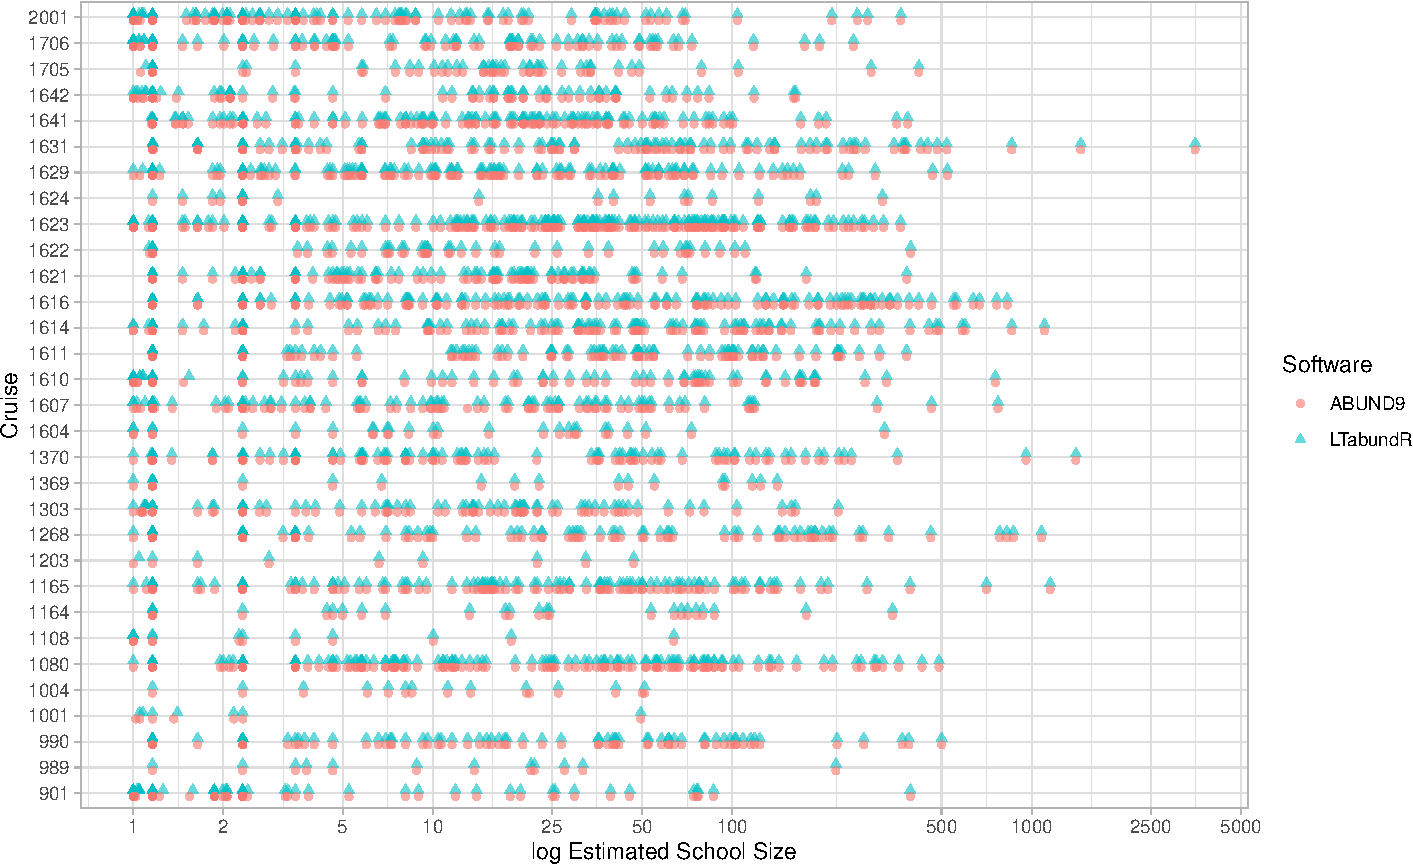
\includegraphics{figures/unnamed-chunk-125-1.pdf}

\hypertarget{effort}{%
\subsection*{Effort}\label{effort}}
\addcontentsline{toc}{subsection}{Effort}

\begin{Shaded}
\begin{Highlighting}[]
\CommentTok{\# Format ABUND}
\NormalTok{abund }\OtherTok{\textless{}{-}} 
\NormalTok{  EFFORT }\SpecialCharTok{\%\textgreater{}\%} 
  \FunctionTok{mutate}\NormalTok{(}\AttributeTok{Region =} \FunctionTok{gsub}\NormalTok{(}\StringTok{\textquotesingle{} \textquotesingle{}}\NormalTok{,}\StringTok{\textquotesingle{}\textquotesingle{}}\NormalTok{,Region)) }\SpecialCharTok{\%\textgreater{}\%}
  \FunctionTok{mutate}\NormalTok{(}\AttributeTok{dt =} \FunctionTok{paste0}\NormalTok{(Yr,}
\NormalTok{                     stringr}\SpecialCharTok{::}\FunctionTok{str\_pad}\NormalTok{(Mo, }\AttributeTok{width=}\DecValTok{2}\NormalTok{, }\AttributeTok{pad=}\StringTok{\textquotesingle{}0\textquotesingle{}}\NormalTok{, }\AttributeTok{side=}\StringTok{\textquotesingle{}left\textquotesingle{}}\NormalTok{),}
\NormalTok{                     stringr}\SpecialCharTok{::}\FunctionTok{str\_pad}\NormalTok{(Da, }\AttributeTok{width=}\DecValTok{2}\NormalTok{, }\AttributeTok{pad=}\StringTok{\textquotesingle{}0\textquotesingle{}}\NormalTok{, }\AttributeTok{side=}\StringTok{\textquotesingle{}left\textquotesingle{}}\NormalTok{))) }\SpecialCharTok{\%\textgreater{}\%} 
  \FunctionTok{filter}\NormalTok{(}\SpecialCharTok{!}\NormalTok{ Region }\SpecialCharTok{\%in\%} \FunctionTok{c}\NormalTok{(}\StringTok{\textquotesingle{}NONE\textquotesingle{}}\NormalTok{, }\StringTok{\textquotesingle{}Off{-}Transect\textquotesingle{}}\NormalTok{),}
\NormalTok{         EffortSeg }\SpecialCharTok{\textgreater{}} \DecValTok{0}\NormalTok{) }\SpecialCharTok{\%\textgreater{}\%} 
  \FunctionTok{select}\NormalTok{(}\AttributeTok{Cruise =}\NormalTok{ CruzNo, }\AttributeTok{Date =}\NormalTok{ dt, }\AttributeTok{km =}\NormalTok{ length) }\SpecialCharTok{\%\textgreater{}\%} 
  \FunctionTok{mutate}\NormalTok{(}\AttributeTok{software =} \StringTok{\textquotesingle{}ABUND9\textquotesingle{}}\NormalTok{)}
  
\CommentTok{\# Format LTabundR}
\NormalTok{ltabundr }\OtherTok{\textless{}{-}} 
\NormalTok{  cruz}\SpecialCharTok{$}\NormalTok{cohorts}\SpecialCharTok{$}\NormalTok{all}\SpecialCharTok{$}\NormalTok{segments }\SpecialCharTok{\%\textgreater{}\%} 
  \FunctionTok{mutate}\NormalTok{(}\AttributeTok{dt =} \FunctionTok{gsub}\NormalTok{(}\StringTok{\textquotesingle{}{-}\textquotesingle{}}\NormalTok{,}\StringTok{\textquotesingle{}\textquotesingle{}}\NormalTok{,}\FunctionTok{substr}\NormalTok{(DateTime1, }\DecValTok{1}\NormalTok{,}\DecValTok{10}\NormalTok{))) }\SpecialCharTok{\%\textgreater{}\%} 
  \FunctionTok{filter}\NormalTok{(OnEffort }\SpecialCharTok{==} \ConstantTok{TRUE}\NormalTok{, }
\NormalTok{         use }\SpecialCharTok{==} \ConstantTok{TRUE}\NormalTok{, }
\NormalTok{         EffType }\SpecialCharTok{\%in\%} \FunctionTok{c}\NormalTok{(}\StringTok{\textquotesingle{}S\textquotesingle{}}\NormalTok{, }\StringTok{\textquotesingle{}F\textquotesingle{}}\NormalTok{)) }\SpecialCharTok{\%\textgreater{}\%} 
  \FunctionTok{select}\NormalTok{(Cruise, }\AttributeTok{Date =}\NormalTok{ dt, }\AttributeTok{km =}\NormalTok{ dist) }\SpecialCharTok{\%\textgreater{}\%} 
  \FunctionTok{mutate}\NormalTok{(}\AttributeTok{software =} \StringTok{\textquotesingle{}LTabundR\textquotesingle{}}\NormalTok{)}
  
\CommentTok{\# Join the datasets}
\NormalTok{eff }\OtherTok{\textless{}{-}} 
  \FunctionTok{rbind}\NormalTok{(abund, ltabundr) }\SpecialCharTok{\%\textgreater{}\%} 
  \FunctionTok{group\_by}\NormalTok{(Cruise) }\SpecialCharTok{\%\textgreater{}\%} 
  \FunctionTok{mutate}\NormalTok{(}\AttributeTok{km =} \FunctionTok{round}\NormalTok{(km)) }\SpecialCharTok{\%\textgreater{}\%} 
  \FunctionTok{summarize}\NormalTok{(}\AttributeTok{km\_abund =} \FunctionTok{sum}\NormalTok{(km[software }\SpecialCharTok{==} \StringTok{\textquotesingle{}ABUND9\textquotesingle{}}\NormalTok{]),}
            \AttributeTok{km\_ltabundr =} \FunctionTok{sum}\NormalTok{(km[software }\SpecialCharTok{==} \StringTok{\textquotesingle{}LTabundR\textquotesingle{}}\NormalTok{]))}

\CommentTok{\# Plot}
\NormalTok{p }\OtherTok{\textless{}{-}} 
  \FunctionTok{ggplot}\NormalTok{(eff, }\FunctionTok{aes}\NormalTok{(}\AttributeTok{x =}\NormalTok{ km\_abund, }\AttributeTok{y =}\NormalTok{ km\_ltabundr, }\AttributeTok{col=}\FunctionTok{factor}\NormalTok{(Cruise))) }\SpecialCharTok{+}
  \FunctionTok{geom\_abline}\NormalTok{(}\AttributeTok{slope=}\DecValTok{1}\NormalTok{, }\AttributeTok{intercept=}\DecValTok{0}\NormalTok{, }\AttributeTok{lty=}\DecValTok{3}\NormalTok{) }\SpecialCharTok{+} 
  \FunctionTok{geom\_point}\NormalTok{(}\AttributeTok{alpha=}\NormalTok{.}\DecValTok{6}\NormalTok{) }\SpecialCharTok{+} 
  \FunctionTok{ylab}\NormalTok{(}\StringTok{\textquotesingle{}LTabundR\textquotesingle{}}\NormalTok{) }\SpecialCharTok{+} \FunctionTok{xlab}\NormalTok{(}\StringTok{\textquotesingle{}ABUND9\textquotesingle{}}\NormalTok{) }\SpecialCharTok{+} 
  \FunctionTok{scale\_x\_continuous}\NormalTok{(}\AttributeTok{breaks =} \FunctionTok{seq}\NormalTok{(}\DecValTok{0}\NormalTok{, }\DecValTok{15000}\NormalTok{, }\AttributeTok{by=}\DecValTok{2500}\NormalTok{)) }\SpecialCharTok{+} 
  \FunctionTok{scale\_y\_continuous}\NormalTok{(}\AttributeTok{breaks =} \FunctionTok{seq}\NormalTok{(}\DecValTok{0}\NormalTok{, }\DecValTok{15000}\NormalTok{, }\AttributeTok{by=}\DecValTok{2500}\NormalTok{)) }\SpecialCharTok{+} 
  \FunctionTok{labs}\NormalTok{(}\AttributeTok{title=}\StringTok{\textquotesingle{}Systematic effort per cruise\textquotesingle{}}\NormalTok{, }\AttributeTok{col=}\StringTok{\textquotesingle{}Cruise\textquotesingle{}}\NormalTok{) }\SpecialCharTok{+} 
  \FunctionTok{theme\_light}\NormalTok{()}

\CommentTok{\# Make it interactive}
\FunctionTok{ggplotly}\NormalTok{(p)}
\end{Highlighting}
\end{Shaded}

\hypertarget{part-data-exploration}{%
\part{Data exploration}\label{part-data-exploration}}

\hypertarget{maps}{%
\chapter{Maps}\label{maps}}

To build a flexible system for mapping cruise data, we have the following functions:

\hypertarget{publishable-maps}{%
\section*{Publishable maps}\label{publishable-maps}}
\addcontentsline{toc}{section}{Publishable maps}

\hypertarget{base-maps}{%
\subsection*{Base maps}\label{base-maps}}
\addcontentsline{toc}{subsection}{Base maps}

Begin with a basic map, including EEZ borders:

\begin{Shaded}
\begin{Highlighting}[]
\NormalTok{m }\OtherTok{\textless{}{-}} \FunctionTok{map\_base}\NormalTok{(}\AttributeTok{region=}\StringTok{\textquotesingle{}cnp\textquotesingle{}}\NormalTok{)}
\NormalTok{m}
\end{Highlighting}
\end{Shaded}

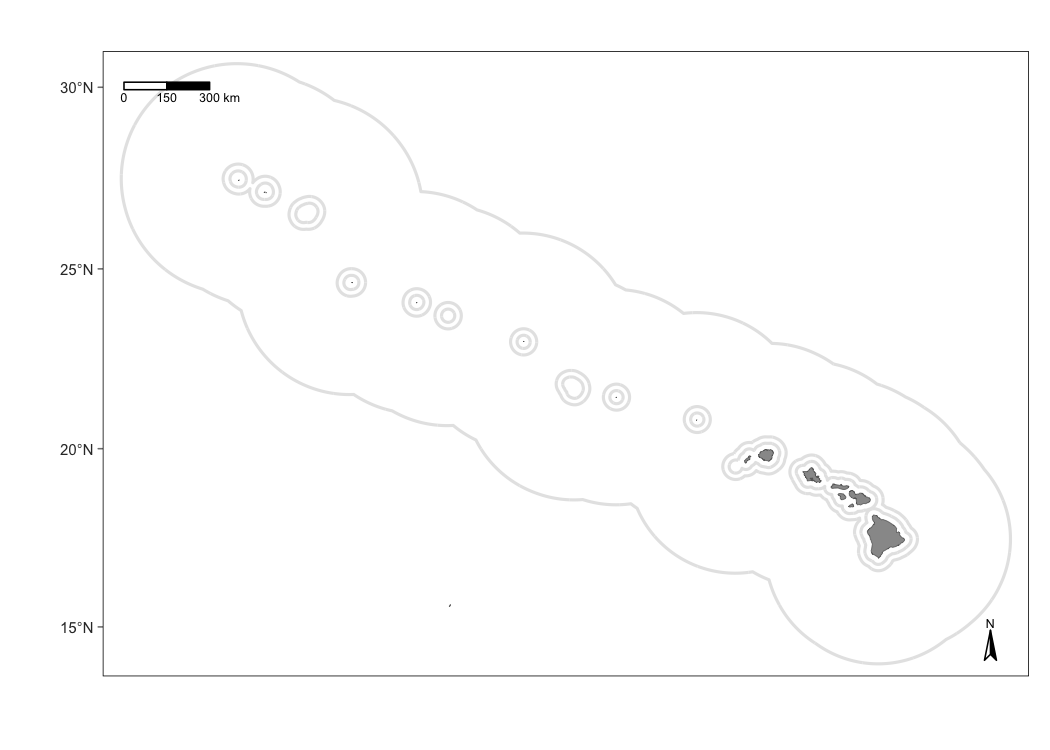
\includegraphics[width=0.95\textwidth,height=\textheight]{img/map_cnp.png}

We also have a base map for the California Current \ldots{}

\begin{Shaded}
\begin{Highlighting}[]
\NormalTok{m }\OtherTok{\textless{}{-}} \FunctionTok{map\_base}\NormalTok{(}\AttributeTok{region=}\StringTok{\textquotesingle{}ccs\textquotesingle{}}\NormalTok{)}
\NormalTok{m}
\end{Highlighting}
\end{Shaded}

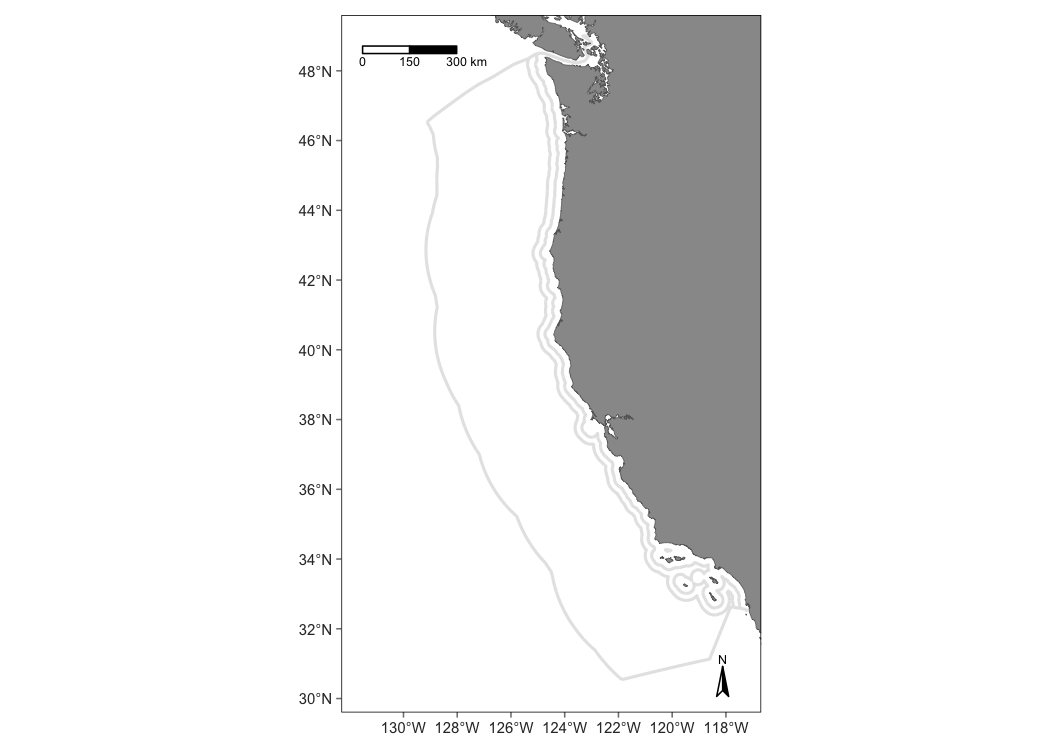
\includegraphics[width=0.95\textwidth,height=\textheight]{img/map_ccs.png}

And the ETP:

\begin{Shaded}
\begin{Highlighting}[]
\NormalTok{m }\OtherTok{\textless{}{-}} \FunctionTok{map\_base}\NormalTok{(}\AttributeTok{region=}\StringTok{\textquotesingle{}etp\textquotesingle{}}\NormalTok{)}
\NormalTok{m}
\end{Highlighting}
\end{Shaded}

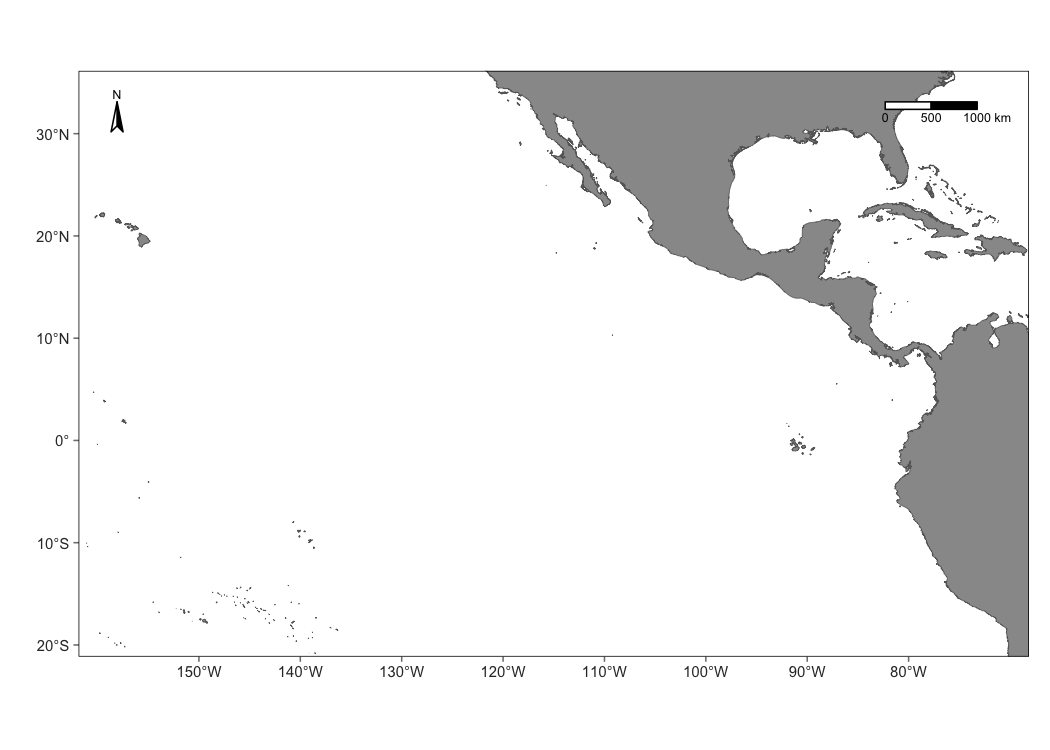
\includegraphics[width=0.95\textwidth,height=\textheight]{img/map_etp.png}

\hypertarget{add-strata}{%
\subsection*{Add strata}\label{add-strata}}
\addcontentsline{toc}{subsection}{Add strata}

Add your research strata to your map:

\begin{Shaded}
\begin{Highlighting}[]
\NormalTok{m }\OtherTok{\textless{}{-}} \FunctionTok{map\_base}\NormalTok{(}\AttributeTok{region=}\StringTok{\textquotesingle{}cnp\textquotesingle{}}\NormalTok{)}
\end{Highlighting}
\end{Shaded}

\begin{Shaded}
\begin{Highlighting}[]
\NormalTok{m1 }\OtherTok{\textless{}{-}} \FunctionTok{map\_strata}\NormalTok{(m,}
\NormalTok{                cruz\_1720}\SpecialCharTok{$}\NormalTok{settings, }
                \AttributeTok{region=}\StringTok{\textquotesingle{}cnp\textquotesingle{}}\NormalTok{)}
\end{Highlighting}
\end{Shaded}

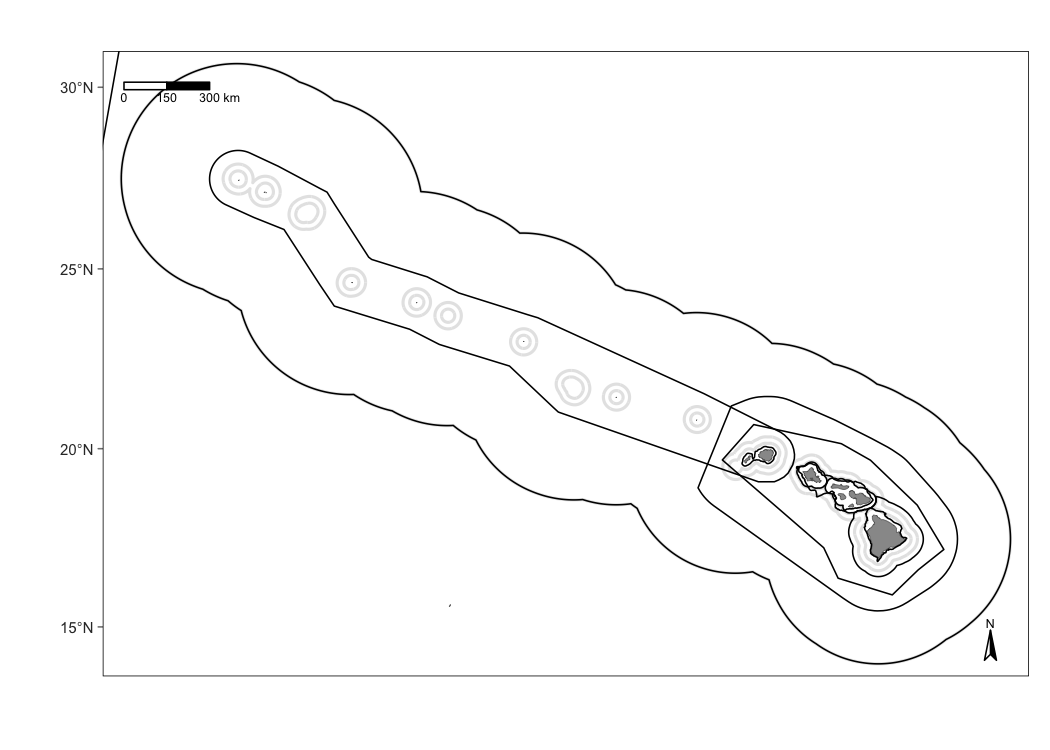
\includegraphics[width=0.95\textwidth,height=\textheight]{img/map_cnp_strata.png}

\hypertarget{add-survey-tracks}{%
\subsection*{Add survey tracks}\label{add-survey-tracks}}
\addcontentsline{toc}{subsection}{Add survey tracks}

\begin{Shaded}
\begin{Highlighting}[]
\NormalTok{m1 }\OtherTok{\textless{}{-}} \FunctionTok{map\_effort}\NormalTok{(m, cruz\_1720)}
\NormalTok{m1}
\end{Highlighting}
\end{Shaded}

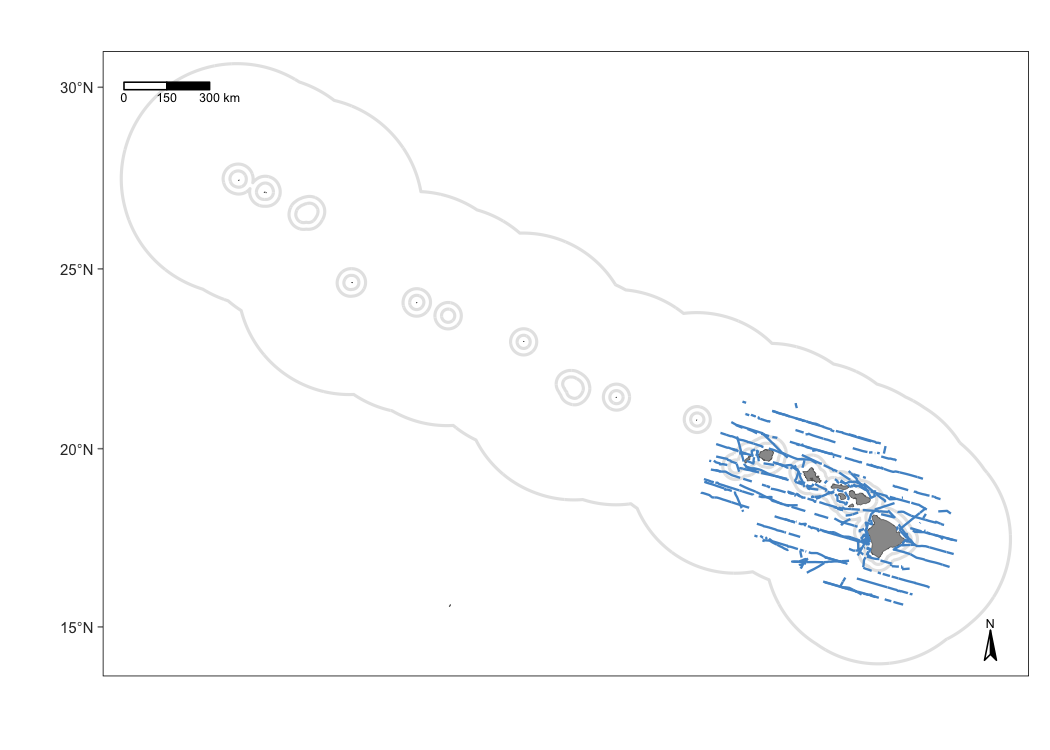
\includegraphics[width=0.95\textwidth,height=\textheight]{img/map_tracks.png}

The defaults of \texttt{map\_effort()} assume, for simplicity, that you want to see the segments to be included in density estimation for the first cohort specified in your settings. You can adjust this and other defaults using the function arguments.

\hypertarget{customizing-effort}{%
\subsubsection*{Customizing effort}\label{customizing-effort}}
\addcontentsline{toc}{subsubsection}{Customizing effort}

\hypertarget{inputs}{%
\paragraph*{Inputs}\label{inputs}}
\addcontentsline{toc}{paragraph}{Inputs}

This map changes survey track thickness and color.

\begin{Shaded}
\begin{Highlighting}[]
\NormalTok{m1 }\OtherTok{\textless{}{-}} \FunctionTok{map\_effort}\NormalTok{(m, }
\NormalTok{                cruz\_1720,}
                \AttributeTok{effort\_color=}\StringTok{\textquotesingle{}firebrick\textquotesingle{}}\NormalTok{,}
                \AttributeTok{effort\_stroke=}\FloatTok{2.5}\NormalTok{,}
                \AttributeTok{effort\_linetype=}\DecValTok{1}\NormalTok{,)}
\end{Highlighting}
\end{Shaded}

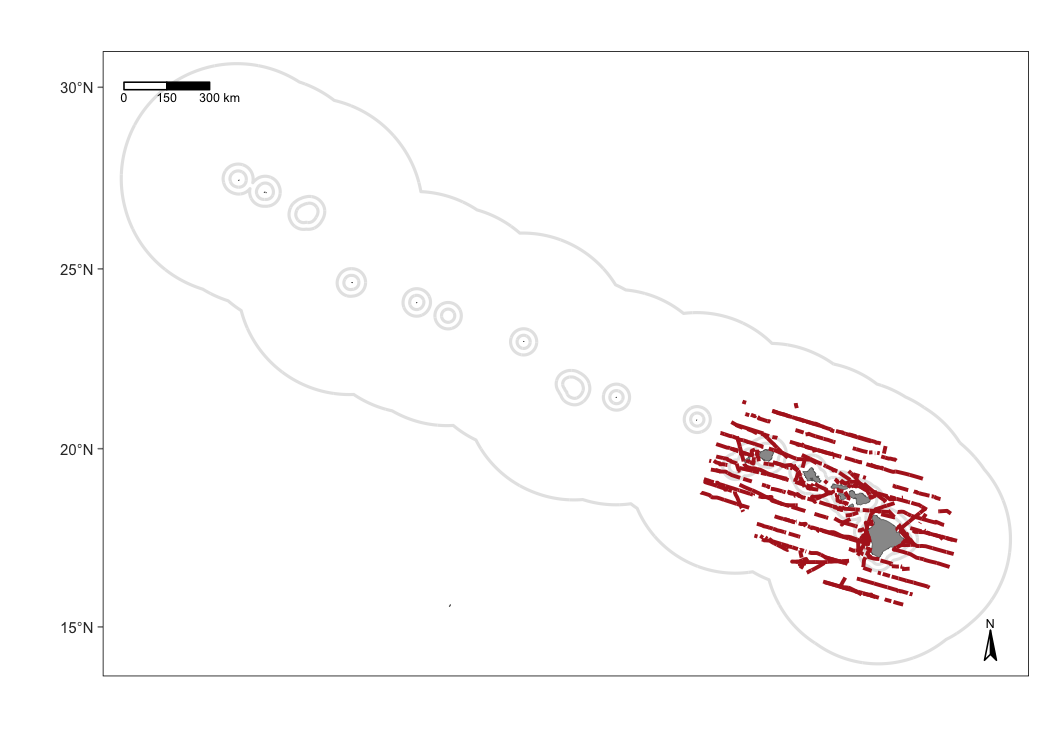
\includegraphics[width=0.95\textwidth,height=\textheight]{img/map_tracks2.png}

\hypertarget{color-code-conditions}{%
\paragraph*{Color-code conditions}\label{color-code-conditions}}
\addcontentsline{toc}{paragraph}{Color-code conditions}

Your second customization option is to add format variables to the \texttt{segments} slot of the cohort of interest in the \texttt{cruz} object. This gives you full control of line color, thickness, and line-type according to whatever specifications you wish to set, e.g., color-coding by effort type or Beaufort sea state.

This is possible because the function \texttt{map\_effort()} looks for the variables \texttt{col} (line color), \texttt{lwd} (line thickness or stroke), and \texttt{lty} (line type) in the columns of \texttt{cruz\$segments}. If these columns exist, the values therein will be used instead of the function defaults.

For example, color-code by Beaufort scale:

\begin{Shaded}
\begin{Highlighting}[]
\CommentTok{\# Save copy of segments to modify}
\NormalTok{cruzi }\OtherTok{\textless{}{-}}\NormalTok{ cruz\_1720}
\NormalTok{segments }\OtherTok{\textless{}{-}}\NormalTok{ cruzi}\SpecialCharTok{$}\NormalTok{cohorts}\SpecialCharTok{$}\NormalTok{all}\SpecialCharTok{$}\NormalTok{segments}

\CommentTok{\# Add column \textasciigrave{}col\textasciigrave{}: color code by BFT sea state}
\NormalTok{bft\_colors }\OtherTok{\textless{}{-}} \FunctionTok{c}\NormalTok{(}\StringTok{\textquotesingle{}steelblue4\textquotesingle{}}\NormalTok{,}\StringTok{\textquotesingle{}steelblue2\textquotesingle{}}\NormalTok{,}\StringTok{\textquotesingle{}cadetblue1\textquotesingle{}}\NormalTok{,}\StringTok{\textquotesingle{}grey\textquotesingle{}}\NormalTok{)}
\NormalTok{segments}\SpecialCharTok{$}\NormalTok{col }\OtherTok{\textless{}{-}}\NormalTok{ bft\_colors[}\DecValTok{4}\NormalTok{]}
\NormalTok{segments}\SpecialCharTok{$}\NormalTok{col[ segments}\SpecialCharTok{$}\NormalTok{avgBft }\SpecialCharTok{\textless{}=} \DecValTok{7}\NormalTok{ ] }\OtherTok{\textless{}{-}}\NormalTok{ bft\_colors[}\DecValTok{3}\NormalTok{] }\CommentTok{\# bft 5 +}
\NormalTok{segments}\SpecialCharTok{$}\NormalTok{col[ segments}\SpecialCharTok{$}\NormalTok{avgBft }\SpecialCharTok{\textless{}=} \DecValTok{4}\NormalTok{ ] }\OtherTok{\textless{}{-}}\NormalTok{ bft\_colors[}\DecValTok{2}\NormalTok{] }\CommentTok{\# bft 3 {-} 4}
\NormalTok{segments}\SpecialCharTok{$}\NormalTok{col[ segments}\SpecialCharTok{$}\NormalTok{avgBft }\SpecialCharTok{\textless{}=} \DecValTok{2}\NormalTok{ ] }\OtherTok{\textless{}{-}}\NormalTok{ bft\_colors[}\DecValTok{1}\NormalTok{] }\CommentTok{\# bft 0 {-}2}

\CommentTok{\# Update sub\_segments slot in \textasciigrave{}cruz\textasciigrave{} object}
\NormalTok{cruzi}\SpecialCharTok{$}\NormalTok{cohorts}\SpecialCharTok{$}\NormalTok{all}\SpecialCharTok{$}\NormalTok{segments }\OtherTok{\textless{}{-}}\NormalTok{ segments}

\CommentTok{\# Update map }
\NormalTok{m\_custom2 }\OtherTok{\textless{}{-}} \FunctionTok{map\_effort}\NormalTok{(m, cruzi)}

\CommentTok{\# Add legend using native functions from mapping package \textasciigrave{}tmap\textasciigrave{}}
\NormalTok{m\_custom2 }\OtherTok{\textless{}{-}} 
\NormalTok{  m\_custom2 }\SpecialCharTok{+} 
\NormalTok{  tmap}\SpecialCharTok{::}\FunctionTok{tm\_add\_legend}\NormalTok{(}\StringTok{\textquotesingle{}line\textquotesingle{}}\NormalTok{, }
                        \AttributeTok{col =}\NormalTok{ bft\_colors,}
                        \AttributeTok{lwd =} \DecValTok{3}\NormalTok{,}
                        \AttributeTok{labels =} \FunctionTok{c}\NormalTok{(}\StringTok{\textquotesingle{} 0 {-} 2\textquotesingle{}}\NormalTok{, }
                                   \StringTok{\textquotesingle{} 3 {-} 4\textquotesingle{}}\NormalTok{, }
                                   \StringTok{\textquotesingle{} 5 +\textquotesingle{}}\NormalTok{, }
                                   \StringTok{\textquotesingle{} no data\textquotesingle{}}\NormalTok{),}
                         \AttributeTok{title=}\StringTok{"Beaufort sea state"}\NormalTok{) }\SpecialCharTok{+}
\NormalTok{  tmap}\SpecialCharTok{::}\FunctionTok{tm\_layout}\NormalTok{(}\AttributeTok{legend.position=}\FunctionTok{c}\NormalTok{(}\StringTok{\textquotesingle{}left\textquotesingle{}}\NormalTok{,}\StringTok{\textquotesingle{}bottom\textquotesingle{}}\NormalTok{))}

\CommentTok{\# Show map}
\NormalTok{m\_custom2}
\end{Highlighting}
\end{Shaded}

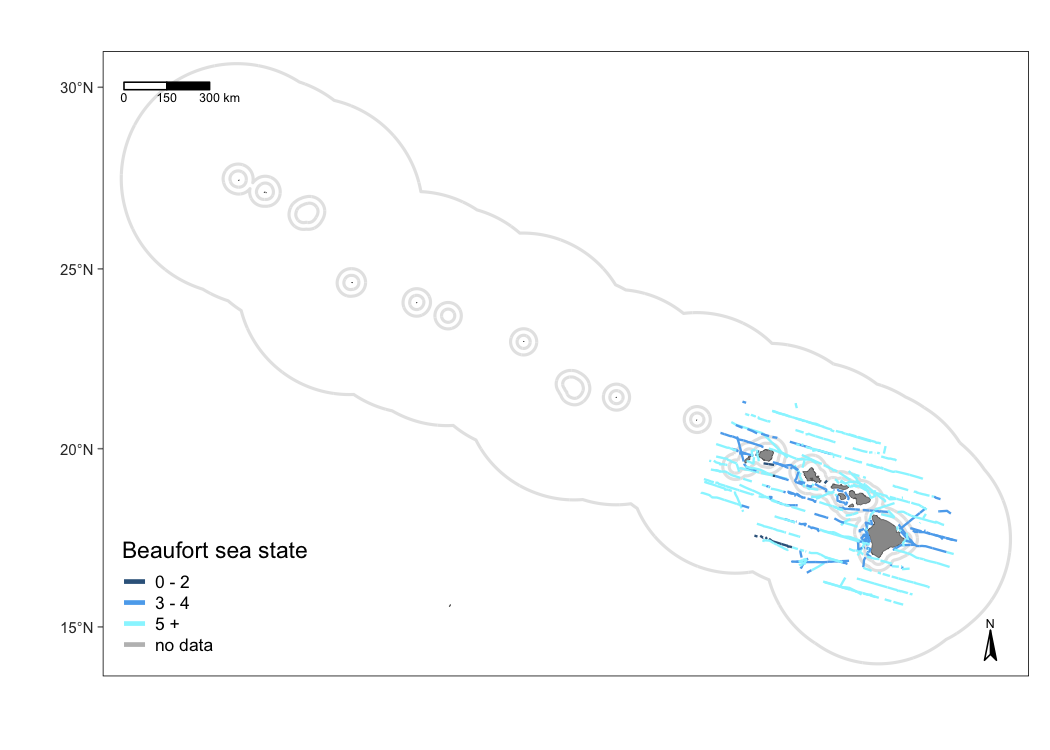
\includegraphics[width=0.95\textwidth,height=\textheight]{img/map_tracks3.png}

\hypertarget{add-sightings}{%
\subsection*{Add sightings}\label{add-sightings}}
\addcontentsline{toc}{subsection}{Add sightings}

Use the function \texttt{map\_sightings()} to add sightings to your map:

\begin{Shaded}
\begin{Highlighting}[]
\NormalTok{m1 }\OtherTok{\textless{}{-}} \FunctionTok{map\_sightings}\NormalTok{(m, cruz\_1720)}
\end{Highlighting}
\end{Shaded}

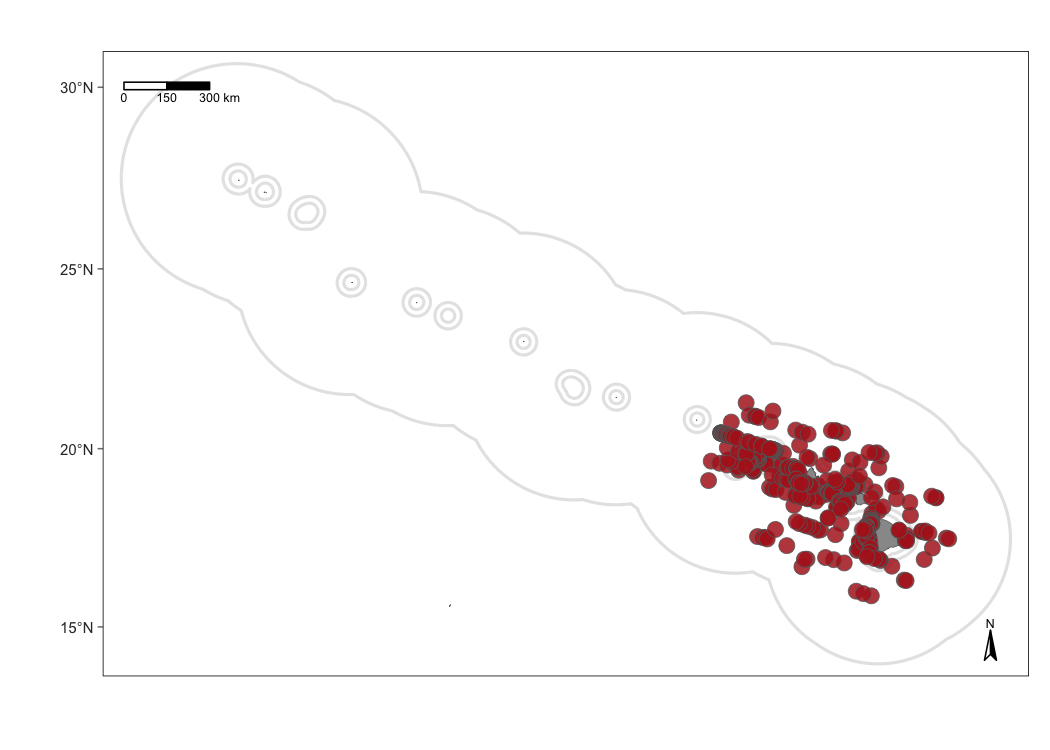
\includegraphics[width=0.95\textwidth,height=\textheight]{img/map_sits.png}

\hypertarget{customizing-sightings}{%
\subsubsection*{Customizing sightings}\label{customizing-sightings}}
\addcontentsline{toc}{subsubsection}{Customizing sightings}

To demonstrate some of the customization options, consider this map that shows sightings of false killer whales with custom dot color, shape, and size:

\begin{Shaded}
\begin{Highlighting}[]
\NormalTok{m1 }\OtherTok{\textless{}{-}} \FunctionTok{map\_sightings}\NormalTok{(m,}
\NormalTok{                    cruz\_1720,}
                    \AttributeTok{include\_species =} \StringTok{\textquotesingle{}033\textquotesingle{}}\NormalTok{,}
                    \AttributeTok{color\_base =} \StringTok{\textquotesingle{}purple\textquotesingle{}}\NormalTok{,}
                    \AttributeTok{shape\_base =} \DecValTok{18}\NormalTok{,}
                    \AttributeTok{size\_base =} \DecValTok{1}\NormalTok{)}
\end{Highlighting}
\end{Shaded}

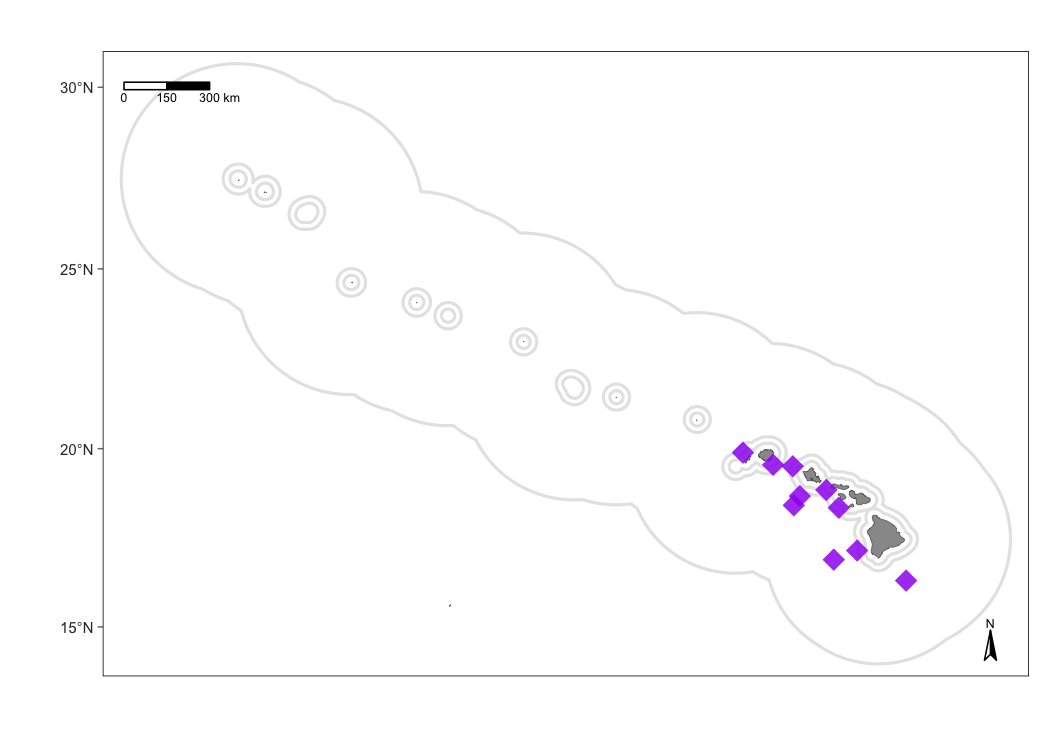
\includegraphics[width=0.95\textwidth,height=\textheight]{img/map_sits2.png}

Next is a map of humpback whales and sperm whales, color-coded by species and shape-coded by whether or not the sighting will be included in the analysis:

\begin{Shaded}
\begin{Highlighting}[]
\NormalTok{m1 }\OtherTok{\textless{}{-}} \FunctionTok{map\_sightings}\NormalTok{(m, }
\NormalTok{                   cruz\_1720,}
                   \AttributeTok{include\_species =} \FunctionTok{c}\NormalTok{(}\StringTok{\textquotesingle{}076\textquotesingle{}}\NormalTok{,}\StringTok{\textquotesingle{}046\textquotesingle{}}\NormalTok{),}
                   \AttributeTok{color\_code =} \ConstantTok{TRUE}\NormalTok{,}
                   \AttributeTok{shape\_code =} \ConstantTok{TRUE}\NormalTok{)}
\end{Highlighting}
\end{Shaded}

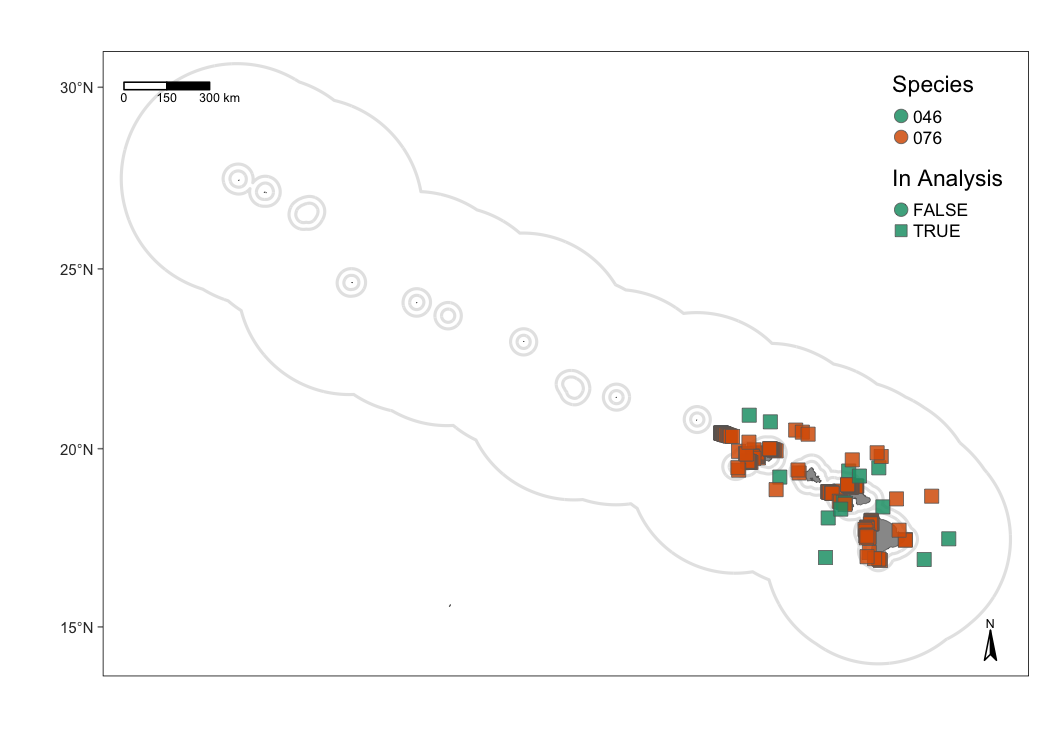
\includegraphics[width=0.95\textwidth,height=\textheight]{img/map_sits3.png}

\hypertarget{overview-1}{%
\subsection*{Overview}\label{overview-1}}
\addcontentsline{toc}{subsection}{Overview}

Here is an overview of the steps needed to map strata, survey tracks, and sightings all together:

\begin{Shaded}
\begin{Highlighting}[]
\NormalTok{m }\OtherTok{\textless{}{-}} \FunctionTok{map\_base}\NormalTok{(}\StringTok{\textquotesingle{}cnp\textquotesingle{}}\NormalTok{) }
\NormalTok{m }\OtherTok{\textless{}{-}} \FunctionTok{map\_strata}\NormalTok{(m, cruz\_1720}\SpecialCharTok{$}\NormalTok{settings)}
\NormalTok{m }\OtherTok{\textless{}{-}} \FunctionTok{map\_effort}\NormalTok{(m, cruz\_1720)}
\NormalTok{m }\OtherTok{\textless{}{-}} \FunctionTok{map\_sightings}\NormalTok{(m, cruz\_1720, }\AttributeTok{size\_base=}\NormalTok{.}\DecValTok{4}\NormalTok{)}
\NormalTok{m }
\end{Highlighting}
\end{Shaded}

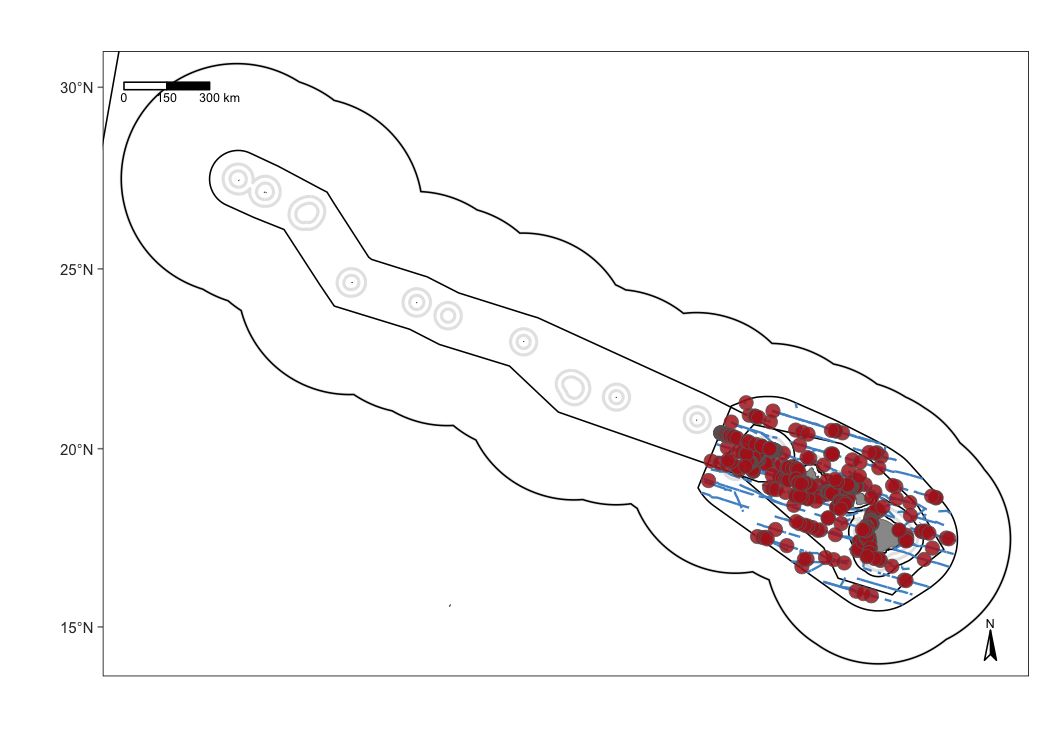
\includegraphics[width=0.95\textwidth,height=\textheight]{img/map_overview.png}

\hypertarget{interactive-maps}{%
\section*{Interactive maps}\label{interactive-maps}}
\addcontentsline{toc}{section}{Interactive maps}

\texttt{LTabundR} also has an interactive map function, which maps survey data using the \texttt{leaflet} package.

\begin{Shaded}
\begin{Highlighting}[]
 \FunctionTok{map\_cruz}\NormalTok{(cruz\_1720,}
          \AttributeTok{cohort=}\DecValTok{1}\NormalTok{,}
          \AttributeTok{eez\_show=}\ConstantTok{FALSE}\NormalTok{,}
          \AttributeTok{strata\_show=}\ConstantTok{FALSE}\NormalTok{,}
          \AttributeTok{effort\_show=}\ConstantTok{TRUE}\NormalTok{,}
          \AttributeTok{effort\_resolution=}\DecValTok{1}\NormalTok{,}
          \AttributeTok{sightings\_show=}\ConstantTok{TRUE}\NormalTok{,}
          \AttributeTok{sightings\_color =} \StringTok{\textquotesingle{}firebrick\textquotesingle{}}\NormalTok{,}
          \AttributeTok{verbose=}\ConstantTok{FALSE}\NormalTok{)}
\end{Highlighting}
\end{Shaded}

Note that you can also click on sightings and tracklines to see their details. Refer to the documentation for this function (\texttt{?map\_cruz}) to see all the options available for stylizing these maps.

\hypertarget{interactive-dashboard}{%
\section*{Interactive dashboard}\label{interactive-dashboard}}
\addcontentsline{toc}{section}{Interactive dashboard}

Finally, note that \texttt{LTabundR} comes with an interactive data explorer app (a \texttt{Shiny} app) for filtering survey data according to effort scenario and species code, toggling \texttt{map\_cruz()} settings, and reviewing summary tables of effort and sightings (including inspection of truncation distances).

\begin{Shaded}
\begin{Highlighting}[]
\FunctionTok{cruz\_explorer}\NormalTok{(cruz)}
\end{Highlighting}
\end{Shaded}

\emph{Screenshots from this app:}

~\\

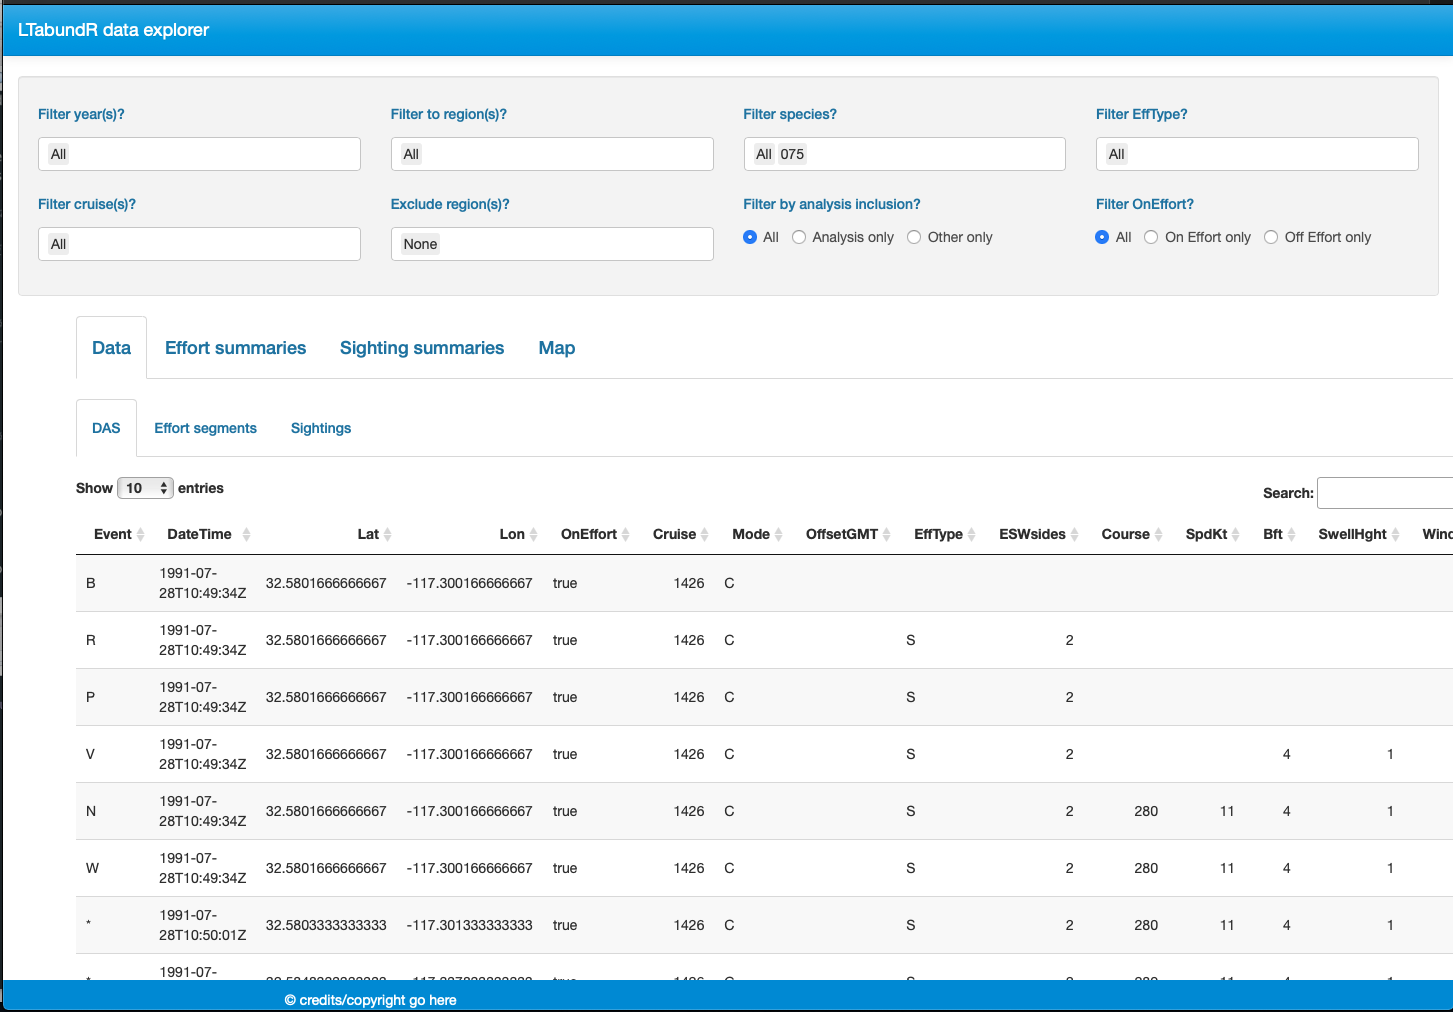
\includegraphics[width=0.85\textwidth,height=\textheight]{img/app-1.png}
~\\
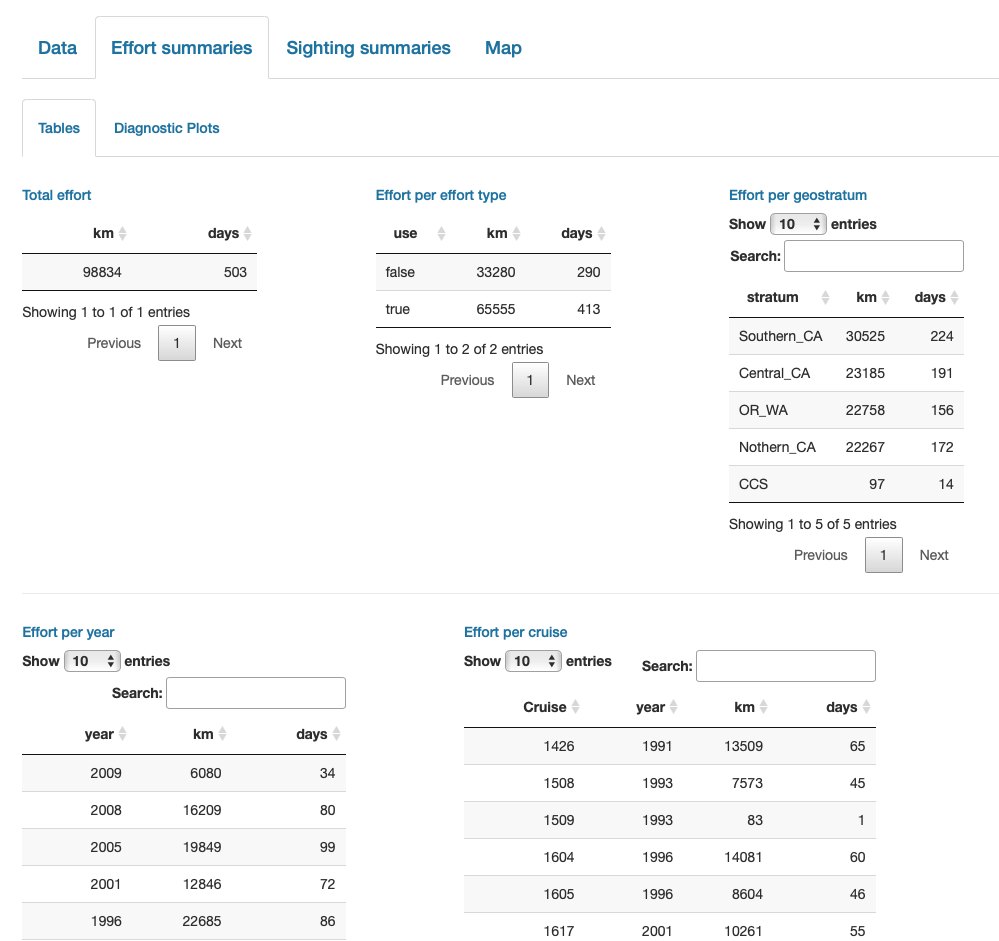
\includegraphics[width=0.85\textwidth,height=\textheight]{img/app-2.png}
~\\
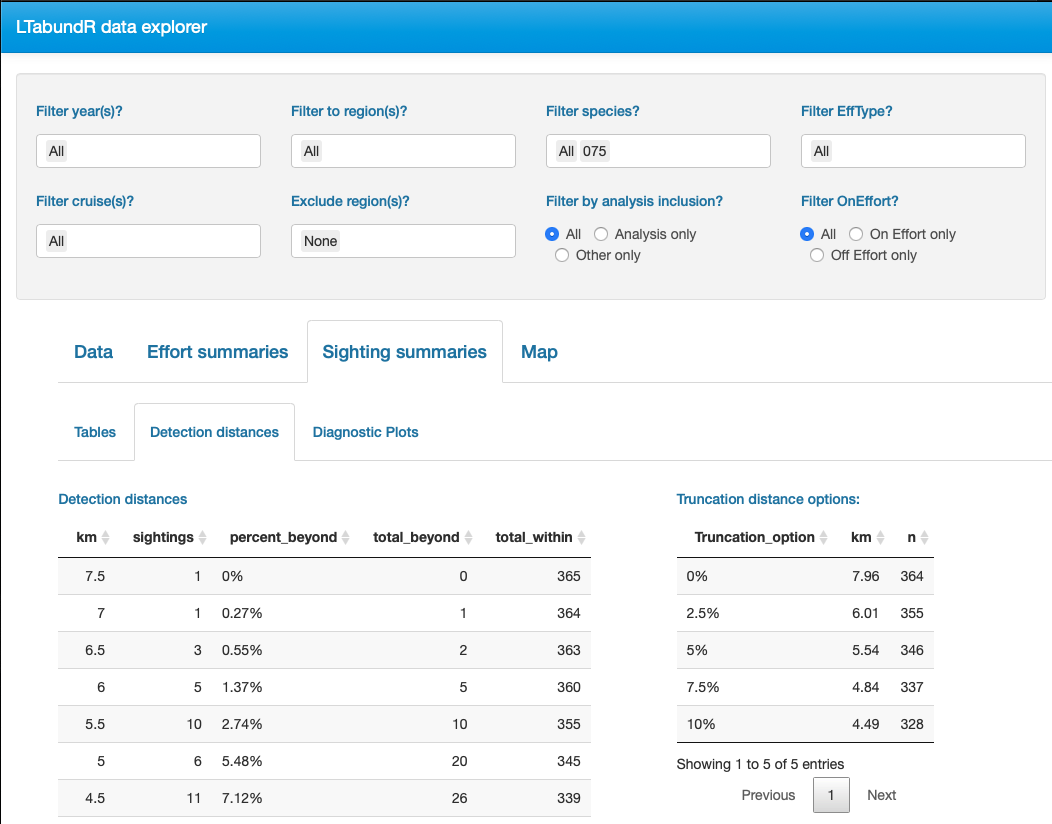
\includegraphics[width=0.85\textwidth,height=\textheight]{img/app-3.png}
~\\
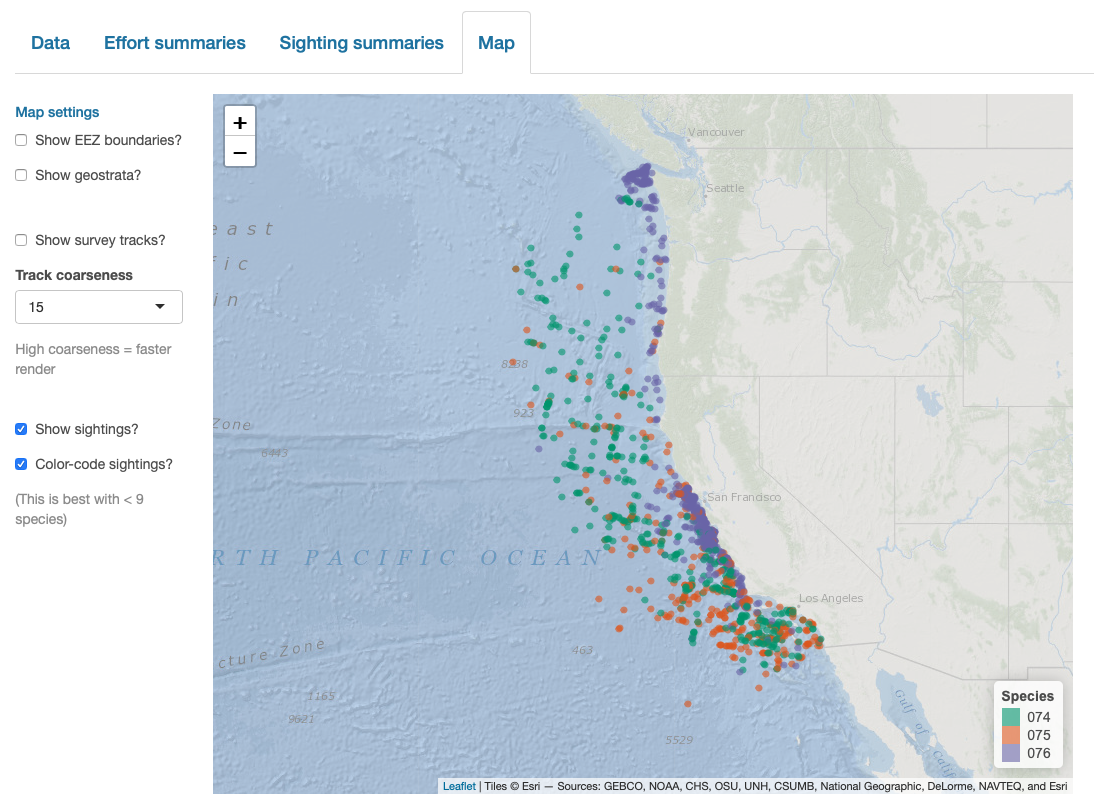
\includegraphics[width=0.85\textwidth,height=\textheight]{img/app-4.png}
~\\
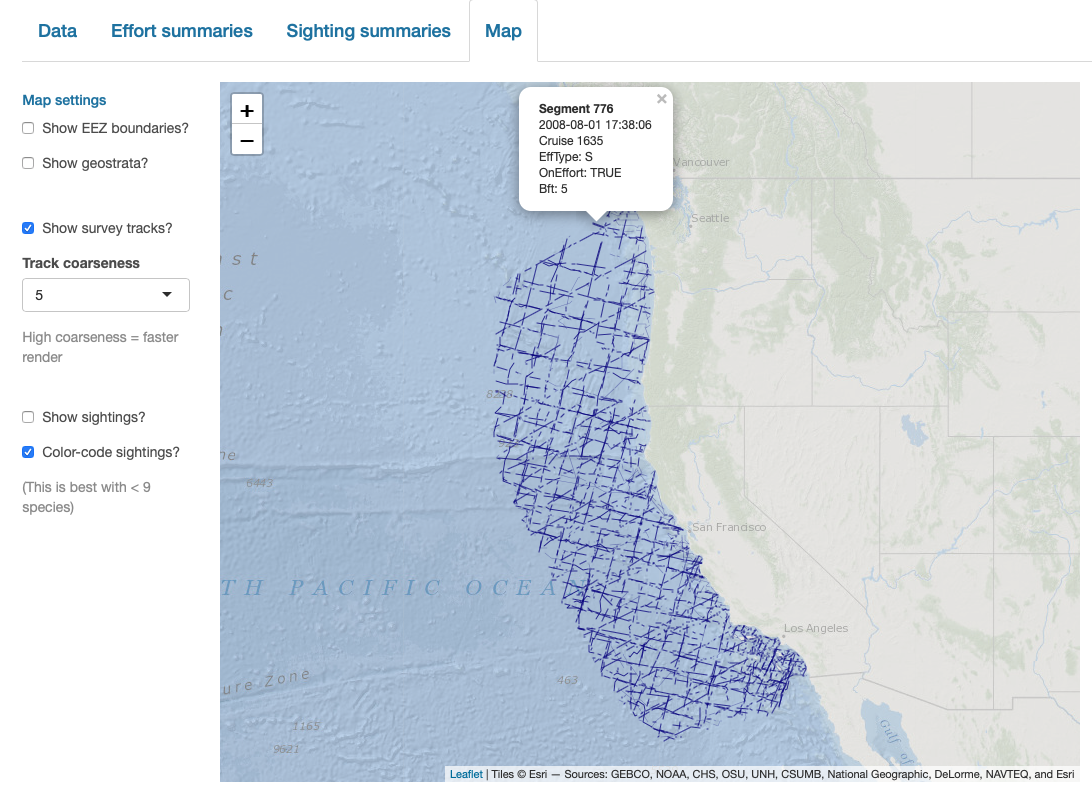
\includegraphics[width=0.85\textwidth,height=\textheight]{img/app-5.png}

\hypertarget{filter}{%
\chapter{Filter \& combine surveys}\label{filter}}

You may soon encounter the need to filter a processed \texttt{cruz} object to only certain years, regions, or cruise numbers. You may also need to combine one processed \texttt{cruz} object with another.

Here we will continue with the \texttt{cruz} object we created on the previous page. As a reminder, here is the data structure of that object:

\begin{Shaded}
\begin{Highlighting}[]
\FunctionTok{cruz\_structure}\NormalTok{(cruz)}
\StringTok{"cruz"}\NormalTok{ list structure }\SpecialCharTok{==}\ErrorTok{======================}

\ErrorTok{$}\NormalTok{settings}
         \SpecialCharTok{$}\NormalTok{strata }\SpecialCharTok{{-}{-}{-}}\NormalTok{ with }\DecValTok{11}\NormalTok{ polygon coordinate sets}
         \SpecialCharTok{$}\NormalTok{survey }\SpecialCharTok{{-}{-}{-}}\NormalTok{ with }\DecValTok{10}\NormalTok{ input arguments}
         \SpecialCharTok{$}\NormalTok{cohorts }\SpecialCharTok{{-}{-}{-}}\NormalTok{ with }\DecValTok{3}\NormalTok{ cohorts specified, each with }\DecValTok{19}\NormalTok{ input arguments}

\SpecialCharTok{$}\NormalTok{strata}
\NormalTok{       ... containing a summary dataframe of }\DecValTok{11}\NormalTok{ geostrata and their spatial areas}
\NormalTok{       ... geostratum names}\SpecialCharTok{:}
\NormalTok{           HI\_EEZ, OtherCNP, MHI, WHICEAS, Spotted\_OU, Spotted\_FI, Spotted\_BI, Bottlenose\_KaNi, Bottlenose\_OUFI, Bottlenose\_BI, NWHI}

\SpecialCharTok{$}\NormalTok{cohorts}

        \SpecialCharTok{$}\NormalTok{all}
\NormalTok{            geostrata}\SpecialCharTok{:}\NormalTok{ WHICEAS, HI\_EEZ, OtherCNP}
            \SpecialCharTok{$}\NormalTok{segments  }\SpecialCharTok{{-}{-}{-}}\NormalTok{ with }\DecValTok{1890} \FunctionTok{segments}\NormalTok{ (}\AttributeTok{median =} \FloatTok{149.3}\NormalTok{ km)}
            \SpecialCharTok{$}\NormalTok{das       }\SpecialCharTok{{-}{-}{-}}\NormalTok{ with }\DecValTok{329632}\NormalTok{ data rows}
            \SpecialCharTok{$}\NormalTok{sightings }\SpecialCharTok{{-}{-}{-}}\NormalTok{ with }\DecValTok{3934}\NormalTok{ detections}
            \SpecialCharTok{$}\NormalTok{subgroups }\SpecialCharTok{{-}{-}{-}}\NormalTok{ with }\DecValTok{255}\NormalTok{ subgroups, }\DecValTok{49}\NormalTok{ sightings, and }\DecValTok{389}\NormalTok{ events}

        \SpecialCharTok{$}\NormalTok{bottlenose}
\NormalTok{            geostrata}\SpecialCharTok{:}\NormalTok{ WHICEAS, HI\_EEZ, OtherCNP, Bottlenose\_BI, Bottlenose\_OUFI, Bottlenose\_KaNi}
            \SpecialCharTok{$}\NormalTok{segments  }\SpecialCharTok{{-}{-}{-}}\NormalTok{ with }\DecValTok{2049} \FunctionTok{segments}\NormalTok{ (}\AttributeTok{median =} \FloatTok{148.6}\NormalTok{ km)}
            \SpecialCharTok{$}\NormalTok{das       }\SpecialCharTok{{-}{-}{-}}\NormalTok{ with }\DecValTok{329632}\NormalTok{ data rows}
            \SpecialCharTok{$}\NormalTok{sightings }\SpecialCharTok{{-}{-}{-}}\NormalTok{ with }\DecValTok{523}\NormalTok{ detections}

        \SpecialCharTok{$}\NormalTok{spotted}
\NormalTok{            geostrata}\SpecialCharTok{:}\NormalTok{ WHICEAS, HI\_EEZ, OtherCNP, Spotted\_OU, Spotted\_FI, Spotted\_BI}
            \SpecialCharTok{$}\NormalTok{segments  }\SpecialCharTok{{-}{-}{-}}\NormalTok{ with }\DecValTok{2057} \FunctionTok{segments}\NormalTok{ (}\AttributeTok{median =} \FloatTok{148.5}\NormalTok{ km)}
            \SpecialCharTok{$}\NormalTok{das       }\SpecialCharTok{{-}{-}{-}}\NormalTok{ with }\DecValTok{329632}\NormalTok{ data rows}
            \SpecialCharTok{$}\NormalTok{sightings }\SpecialCharTok{{-}{-}{-}}\NormalTok{ with }\DecValTok{527}\NormalTok{ detections}
\end{Highlighting}
\end{Shaded}

\hypertarget{filter-1}{%
\section*{Filter}\label{filter-1}}
\addcontentsline{toc}{section}{Filter}

\texttt{LTabundR} lets you filter a \texttt{cruz} object using the function \texttt{filter\_cruz()}.

For example, in our WHICEAS case study, we processed surveys from 1986 - 2020, which we needed to do to model our detection functions, but our interest for mapping is specifically valid effort in 2017 and 2020 only, and only within the \texttt{"WHICEAS"} geostratum.

\begin{Shaded}
\begin{Highlighting}[]
\NormalTok{cruz\_1720 }\OtherTok{\textless{}{-}} 
  \FunctionTok{filter\_cruz}\NormalTok{(cruz,}
              \AttributeTok{analysis\_only =} \ConstantTok{TRUE}\NormalTok{,}
              \AttributeTok{years =} \FunctionTok{c}\NormalTok{(}\DecValTok{2017}\NormalTok{, }\DecValTok{2020}\NormalTok{),}
              \AttributeTok{regions =} \StringTok{\textquotesingle{}WHICEAS\textquotesingle{}}\NormalTok{)}
\end{Highlighting}
\end{Shaded}

We will use this filtered \texttt{cruz} object for mapping \& sightings summaries downstream.

\begin{Shaded}
\begin{Highlighting}[]
\FunctionTok{save}\NormalTok{(cruz\_1720,}\AttributeTok{file=}\StringTok{\textquotesingle{}whiceas\_cruz\_1720.RData\textquotesingle{}}\NormalTok{)}
\end{Highlighting}
\end{Shaded}

Note that \texttt{filter\_cruz()} has many other filter options. See \texttt{?filter\_cruz()} for details.

\hypertarget{combine}{%
\section*{Combine}\label{combine}}
\addcontentsline{toc}{section}{Combine}

Say you have two processed \texttt{cruz} objects: one containing survey effort from the Hawaiian EEZ (\texttt{HI\_EEZ}) geostratum area only, and one containing survey effort from everywhere else that does \emph{not} include \texttt{HI\_EEZ} effort.

Let's make those fake datasets right now, using \texttt{filter\_cruz()}:

\textbf{Hawaiian EEZ-only data:}

\begin{Shaded}
\begin{Highlighting}[]
\NormalTok{cruz\_hi }\OtherTok{\textless{}{-}} \FunctionTok{filter\_cruz}\NormalTok{(cruz, }
                            \AttributeTok{regions =} \StringTok{\textquotesingle{}HI\_EEZ\textquotesingle{}}\NormalTok{, }
                            \AttributeTok{verbose =} \ConstantTok{FALSE}\NormalTok{)}
\end{Highlighting}
\end{Shaded}

\textbf{Pelagic Hawaiian EEZ - only data:}

\begin{Shaded}
\begin{Highlighting}[]
\NormalTok{cruz\_other }\OtherTok{\textless{}{-}} \FunctionTok{filter\_cruz}\NormalTok{(cruz, }
                           \AttributeTok{not\_regions =} \StringTok{\textquotesingle{}HI\_EEZ\textquotesingle{}}\NormalTok{, }
                           \AttributeTok{verbose =} \ConstantTok{FALSE}\NormalTok{)}
\end{Highlighting}
\end{Shaded}

Say you want to combine these datasets together in order to reconstruct the equivalent of our original \texttt{cruz} object. You can do this with the \texttt{LTabundR} function, \texttt{cruz\_combine()}.

\begin{Shaded}
\begin{Highlighting}[]
\CommentTok{\# Make a list of cruz objects}
\NormalTok{cruzes }\OtherTok{\textless{}{-}} \FunctionTok{list}\NormalTok{(cruz\_hi, cruz\_other)}

\CommentTok{\# Now combine}
\NormalTok{cruz\_demo }\OtherTok{\textless{}{-}} \FunctionTok{cruz\_combine}\NormalTok{(cruzes)}
\end{Highlighting}
\end{Shaded}

Re-constituted data structure:

\begin{Shaded}
\begin{Highlighting}[]
\FunctionTok{cruz\_structure}\NormalTok{(cruz\_demo)}
\StringTok{"cruz"}\NormalTok{ list structure }\SpecialCharTok{==}\ErrorTok{======================}

\ErrorTok{$}\NormalTok{settings}
         \SpecialCharTok{$}\NormalTok{strata }\SpecialCharTok{{-}{-}{-}}\NormalTok{ with }\DecValTok{11}\NormalTok{ polygon coordinate sets}
         \SpecialCharTok{$}\NormalTok{survey }\SpecialCharTok{{-}{-}{-}}\NormalTok{ with }\DecValTok{10}\NormalTok{ input arguments}
         \SpecialCharTok{$}\NormalTok{cohorts }\SpecialCharTok{{-}{-}{-}}\NormalTok{ with }\DecValTok{3}\NormalTok{ cohorts specified, each with }\DecValTok{19}\NormalTok{ input arguments}

\SpecialCharTok{$}\NormalTok{strata}
\NormalTok{       ... containing a summary dataframe of }\DecValTok{11}\NormalTok{ geostrata and their spatial areas}
\NormalTok{       ... geostratum names}\SpecialCharTok{:}
\NormalTok{           HI\_EEZ, OtherCNP, MHI, WHICEAS, Spotted\_OU, Spotted\_FI, Spotted\_BI, Bottlenose\_KaNi, Bottlenose\_OUFI, Bottlenose\_BI, NWHI}

\SpecialCharTok{$}\NormalTok{cohorts}

        \SpecialCharTok{$}\NormalTok{all}
\NormalTok{            geostrata}\SpecialCharTok{:}\NormalTok{ WHICEAS, HI\_EEZ, OtherCNP}
            \SpecialCharTok{$}\NormalTok{segments  }\SpecialCharTok{{-}{-}{-}}\NormalTok{ with }\DecValTok{1890} \FunctionTok{segments}\NormalTok{ (}\AttributeTok{median =} \FloatTok{149.3}\NormalTok{ km)}
            \SpecialCharTok{$}\NormalTok{das       }\SpecialCharTok{{-}{-}{-}}\NormalTok{ with }\DecValTok{329632}\NormalTok{ data rows}
            \SpecialCharTok{$}\NormalTok{sightings }\SpecialCharTok{{-}{-}{-}}\NormalTok{ with }\DecValTok{3934}\NormalTok{ detections}
            \SpecialCharTok{$}\NormalTok{subgroups }\SpecialCharTok{{-}{-}{-}}\NormalTok{ with }\DecValTok{237}\NormalTok{ subgroups, }\DecValTok{39}\NormalTok{ sightings, and }\DecValTok{345}\NormalTok{ events}

        \SpecialCharTok{$}\NormalTok{bottlenose}
\NormalTok{            geostrata}\SpecialCharTok{:}\NormalTok{ WHICEAS, HI\_EEZ, OtherCNP, Bottlenose\_BI, Bottlenose\_OUFI, Bottlenose\_KaNi}
            \SpecialCharTok{$}\NormalTok{segments  }\SpecialCharTok{{-}{-}{-}}\NormalTok{ with }\DecValTok{2049} \FunctionTok{segments}\NormalTok{ (}\AttributeTok{median =} \FloatTok{148.6}\NormalTok{ km)}
            \SpecialCharTok{$}\NormalTok{das       }\SpecialCharTok{{-}{-}{-}}\NormalTok{ with }\DecValTok{329632}\NormalTok{ data rows}
            \SpecialCharTok{$}\NormalTok{sightings }\SpecialCharTok{{-}{-}{-}}\NormalTok{ with }\DecValTok{523}\NormalTok{ detections}

        \SpecialCharTok{$}\NormalTok{spotted}
\NormalTok{            geostrata}\SpecialCharTok{:}\NormalTok{ WHICEAS, HI\_EEZ, OtherCNP, Spotted\_OU, Spotted\_FI, Spotted\_BI}
            \SpecialCharTok{$}\NormalTok{segments  }\SpecialCharTok{{-}{-}{-}}\NormalTok{ with }\DecValTok{2057} \FunctionTok{segments}\NormalTok{ (}\AttributeTok{median =} \FloatTok{148.5}\NormalTok{ km)}
            \SpecialCharTok{$}\NormalTok{das       }\SpecialCharTok{{-}{-}{-}}\NormalTok{ with }\DecValTok{329632}\NormalTok{ data rows}
            \SpecialCharTok{$}\NormalTok{sightings }\SpecialCharTok{{-}{-}{-}}\NormalTok{ with }\DecValTok{527}\NormalTok{ detections}
\end{Highlighting}
\end{Shaded}

\hypertarget{summarize}{%
\chapter{Summarize survey}\label{summarize}}

Here we will summarize the 2017 \& 2020 survey data we prepared on the previous page.

\begin{Shaded}
\begin{Highlighting}[]
\FunctionTok{load}\NormalTok{(}\StringTok{\textquotesingle{}whiceas\_cruz\_1720.RData\textquotesingle{}}\NormalTok{)}
\end{Highlighting}
\end{Shaded}

\hypertarget{summarize-effort}{%
\section*{Summarize effort}\label{summarize-effort}}
\addcontentsline{toc}{section}{Summarize effort}

The \texttt{summarize\_effort()} functions builds tables with total kilometers and days surveyed.

\begin{Shaded}
\begin{Highlighting}[]
\NormalTok{effort }\OtherTok{\textless{}{-}} \FunctionTok{summarize\_effort}\NormalTok{(cruz\_1720,}
                           \AttributeTok{cohort=}\DecValTok{1}\NormalTok{)}
\end{Highlighting}
\end{Shaded}

This function summarizes effort in several default tables:

\begin{Shaded}
\begin{Highlighting}[]
\NormalTok{effort }\SpecialCharTok{\%\textgreater{}\%}  \FunctionTok{names}\NormalTok{()}
\NormalTok{[}\DecValTok{1}\NormalTok{] }\StringTok{"total"}            \StringTok{"total\_by\_cruise"}  \StringTok{"total\_by\_year"}    \StringTok{"total\_by\_effort"} 
\NormalTok{[}\DecValTok{5}\NormalTok{] }\StringTok{"total\_by\_stratum"}
\end{Highlighting}
\end{Shaded}

\hypertarget{total-surveyed}{%
\subsubsection*{Total surveyed}\label{total-surveyed}}
\addcontentsline{toc}{subsubsection}{Total surveyed}

The slot \texttt{\$total} provides the grand total distance and unique dates surveyed:

\begin{Shaded}
\begin{Highlighting}[]
\FunctionTok{library}\NormalTok{(DT)}

\NormalTok{effort}\SpecialCharTok{$}\NormalTok{total }\SpecialCharTok{\%\textgreater{}\%} 
\NormalTok{  DT}\SpecialCharTok{::}\FunctionTok{datatable}\NormalTok{(}\AttributeTok{options=}\FunctionTok{list}\NormalTok{(}\AttributeTok{initComplete =}\NormalTok{ htmlwidgets}\SpecialCharTok{::}\FunctionTok{JS}\NormalTok{(}
          \StringTok{"function(settings, json) \{$(this.api().table().container()).css(\{\textquotesingle{}font{-}size\textquotesingle{}: \textquotesingle{}9pt\textquotesingle{}\});\}"}\NormalTok{)}
\NormalTok{       )) }
\end{Highlighting}
\end{Shaded}

\hypertarget{total-surveyed-by-effort}{%
\subsubsection*{Total surveyed by effort}\label{total-surveyed-by-effort}}
\addcontentsline{toc}{subsubsection}{Total surveyed by effort}

The slot \texttt{\$total\_by\_effort} provides the total distance and days surveyed, grouped by segments that will be included in the analysis and those that won't:

\hypertarget{total-surveyed-by-stratum}{%
\subsubsection*{Total surveyed by stratum}\label{total-surveyed-by-stratum}}
\addcontentsline{toc}{subsubsection}{Total surveyed by stratum}

The slot \texttt{\$total\_by\_stratum} provides the total distance and days surveyed within each stratum, again grouped by segments that will be included in the analysis and those that won't:

\hypertarget{summarize-by-beaufort}{%
\section*{Summarize by Beaufort}\label{summarize-by-beaufort}}
\addcontentsline{toc}{section}{Summarize by Beaufort}

\begin{Shaded}
\begin{Highlighting}[]
\NormalTok{bft }\OtherTok{\textless{}{-}} \FunctionTok{summarize\_bft}\NormalTok{(cruz\_1720, }\AttributeTok{cohort=}\DecValTok{1}\NormalTok{)}
\end{Highlighting}
\end{Shaded}

This function summarizes effort by Beaufort in four default tables:

\begin{Shaded}
\begin{Highlighting}[]
\NormalTok{bft }\SpecialCharTok{\%\textgreater{}\%}  \FunctionTok{names}\NormalTok{()}
\NormalTok{[}\DecValTok{1}\NormalTok{] }\StringTok{"overall"}    \StringTok{"by\_year"}    \StringTok{"by\_stratum"} \StringTok{"details"}   
\end{Highlighting}
\end{Shaded}

\hypertarget{simple-overall-breakdown}{%
\subsection*{Simple overall breakdown}\label{simple-overall-breakdown}}
\addcontentsline{toc}{subsection}{Simple overall breakdown}

The slot \texttt{\$overall} provides the total effort -- and proportion of effort -- occurring in each Beaufort state:

\hypertarget{breakdown-by-year}{%
\subsection*{Breakdown by year}\label{breakdown-by-year}}
\addcontentsline{toc}{subsection}{Breakdown by year}

The slot \texttt{\$by\_year} provides the above for each year separately:

\hypertarget{breakdown-by-stratum}{%
\subsection*{Breakdown by stratum}\label{breakdown-by-stratum}}
\addcontentsline{toc}{subsection}{Breakdown by stratum}

The slot \texttt{\$by\_stratum} provides the above for each geostratum separately:

\hypertarget{detailed-breakdown}{%
\subsection*{Detailed breakdown}\label{detailed-breakdown}}
\addcontentsline{toc}{subsection}{Detailed breakdown}

The slot \texttt{\$details} provides the above for each cruise-year-study area-geostratum combination within the data:

\hypertarget{summarize-sightings}{%
\section*{Summarize sightings}\label{summarize-sightings}}
\addcontentsline{toc}{section}{Summarize sightings}

The \texttt{summarize\_sightings()} function builds tables summarizing the sightings within each cohort-analysis. (Eventually, we may want to include an option to merge all sightings from all cohort-analyses into a single table.)

\begin{Shaded}
\begin{Highlighting}[]
\NormalTok{sightings }\OtherTok{\textless{}{-}} \FunctionTok{summarize\_sightings}\NormalTok{(cruz\_1720,}
                                 \AttributeTok{cohort=}\DecValTok{1}\NormalTok{)}
\end{Highlighting}
\end{Shaded}

This function summarizes sightings in four default tables:

\begin{Shaded}
\begin{Highlighting}[]
\NormalTok{sightings }\SpecialCharTok{\%\textgreater{}\%}  \FunctionTok{names}\NormalTok{()}
\NormalTok{[}\DecValTok{1}\NormalTok{] }\StringTok{"simple\_totals"}           \StringTok{"analysis\_totals"}        
\NormalTok{[}\DecValTok{3}\NormalTok{] }\StringTok{"stratum\_simple\_totals"}   \StringTok{"stratum\_analysis\_totals"}
\end{Highlighting}
\end{Shaded}

\hypertarget{simple-species-totals}{%
\subsubsection*{Simple species totals}\label{simple-species-totals}}
\addcontentsline{toc}{subsubsection}{Simple species totals}

The slot \texttt{\$simple\_totals} includes all sightings, even if they will not be inluded in analysis:

\hypertarget{analysis-totals}{%
\subsubsection*{Analysis totals}\label{analysis-totals}}
\addcontentsline{toc}{subsubsection}{Analysis totals}

The slot \texttt{\$analysis\_totals} only includes sightings that meet all inclusion criteria for the analysis:

\hypertarget{simple-totals-for-each-stratum}{%
\subsubsection*{Simple totals for each stratum}\label{simple-totals-for-each-stratum}}
\addcontentsline{toc}{subsubsection}{Simple totals for each stratum}

The slot \texttt{\$stratum\_simple\_totals} splits the first table (simple species totals) so that sightings are tallied for each geo-stratum separately:

\hypertarget{analysis-totals-for-each-stratum}{%
\subsubsection*{Analysis totals for each stratum}\label{analysis-totals-for-each-stratum}}
\addcontentsline{toc}{subsubsection}{Analysis totals for each stratum}

The slot \texttt{\$stratum\_analysis\_totals} splits the second table (analysis totals for each species) so that sightings are tallied for each geo-stratum separately:

\hypertarget{summarize-certain-species}{%
\section*{Summarize certain species}\label{summarize-certain-species}}
\addcontentsline{toc}{section}{Summarize certain species}

To deep-dive into details for a ceratin species (or group of species), use the function \texttt{summarize\_species()}.

\begin{Shaded}
\begin{Highlighting}[]
\NormalTok{species }\OtherTok{\textless{}{-}} \FunctionTok{summarize\_species}\NormalTok{(}\AttributeTok{spp=}\StringTok{\textquotesingle{}046\textquotesingle{}}\NormalTok{, cruz\_1720)}
\end{Highlighting}
\end{Shaded}

This functions a list with a variety of summaries:

\begin{Shaded}
\begin{Highlighting}[]
\NormalTok{species }\SpecialCharTok{\%\textgreater{}\%}\NormalTok{ names}
\NormalTok{ [}\DecValTok{1}\NormalTok{] }\StringTok{"species"}             \StringTok{"n\_total"}             \StringTok{"n\_analysis"}         
\NormalTok{ [}\DecValTok{4}\NormalTok{] }\StringTok{"school\_size"}         \StringTok{"yearly\_total"}        \StringTok{"yearly\_analysis"}    
\NormalTok{ [}\DecValTok{7}\NormalTok{] }\StringTok{"regional\_total"}      \StringTok{"regional\_analysis"}   \StringTok{"detection\_distances"}
\NormalTok{[}\DecValTok{10}\NormalTok{] }\StringTok{"sightings"}          
\end{Highlighting}
\end{Shaded}

The slots \texttt{\$n\_total} and \texttt{\$n\_analysis} provide the total number of sightings and the number eligible for inclusion in the analysis:

\begin{Shaded}
\begin{Highlighting}[]
\NormalTok{species}\SpecialCharTok{$}\NormalTok{n\_total}
\NormalTok{[}\DecValTok{1}\NormalTok{] }\DecValTok{14}
\NormalTok{species}\SpecialCharTok{$}\NormalTok{n\_analysis}
\NormalTok{[}\DecValTok{1}\NormalTok{] }\DecValTok{14}
\end{Highlighting}
\end{Shaded}

\hypertarget{school-size-details}{%
\subsubsection*{School size details}\label{school-size-details}}
\addcontentsline{toc}{subsubsection}{School size details}

This table only includes the sightings eligible for analysis:

\hypertarget{annual-summaries-all-sightings}{%
\subsubsection*{Annual summaries (all sightings)}\label{annual-summaries-all-sightings}}
\addcontentsline{toc}{subsubsection}{Annual summaries (all sightings)}

\hypertarget{annual-summaries-analysis-only}{%
\subsubsection*{Annual summaries (analysis only)}\label{annual-summaries-analysis-only}}
\addcontentsline{toc}{subsubsection}{Annual summaries (analysis only)}

\hypertarget{regional-summaries-all-sightings}{%
\subsubsection*{Regional summaries (all sightings)}\label{regional-summaries-all-sightings}}
\addcontentsline{toc}{subsubsection}{Regional summaries (all sightings)}

\hypertarget{regional-summaries-analysis-only}{%
\subsubsection*{Regional summaries (analysis only)}\label{regional-summaries-analysis-only}}
\addcontentsline{toc}{subsubsection}{Regional summaries (analysis only)}

\hypertarget{detection-distances}{%
\subsubsection*{Detection distances}\label{detection-distances}}
\addcontentsline{toc}{subsubsection}{Detection distances}

This table can be used to determine the best truncation distance to use, based on the
percent truncation you wish and the number of sightings available at each option.

\hypertarget{all-sightings-data}{%
\subsubsection*{All sightings data}\label{all-sightings-data}}
\addcontentsline{toc}{subsubsection}{All sightings data}

Finally, this last slot holds a dataframe of all sightings data for the specified species:

\hypertarget{cruz_explorer}{%
\section*{\texorpdfstring{\texttt{cruz\_explorer()}}{cruz\_explorer()}}\label{cruz_explorer}}
\addcontentsline{toc}{section}{\texttt{cruz\_explorer()}}

Note that all of these summary tables can be viewed interactively using the function \texttt{cruz\_explorer()},
which allows you to efficiently subset the data according to various filters.

\begin{Shaded}
\begin{Highlighting}[]
\FunctionTok{cruz\_explorer}\NormalTok{(cruz\_1720)}
\end{Highlighting}
\end{Shaded}

\hypertarget{part-data-analysis}{%
\part{Data analysis}\label{part-data-analysis}}

\hypertarget{g0}{%
\chapter{Estimating g(0)}\label{g0}}

\textbf{Detection function models assume \emph{g(0)} is 1.0.}\\
In distance sampling, a ``detection function'' is fit to the your sighting distances to reflect the fact that animals farther out are more difficult to detect. That detection function is a model of how the probability of detection declines with increasing distance from your survey trackline. The equations for detection function models are all constructed to assume that the probability of detecting an animal on your trackline (distance = 0 km) is 1.0 -- you never miss an animal on your trackline. This trackline detection probability is referred to as \emph{g(0)}.

\textbf{In reality, though, it almost never is -- and it greatly impacts results.}\\
When searching for marine mammals at sea, even some of those occurring directly on your survey trackline will be missed. Real \emph{g(0)} is actually less than 1.0. This technicality makes a big difference: if \emph{g(0)} is actually 0.5, the assumption that \emph{g(0)} is 1.0 will underestimate animal abundance by 50\%. Some animals, such as pygmy and dwarf sperm whales (Genus \emph{Kogia}), are very cryptic and easily missed, and thus likely have a true \emph{g(0)} below 0.1. This means that estimates assuming their \emph{g(0)} is still 1.0 will underestimate true abundance by 90\%! Moreover, \emph{all} species -- whether you are a pygmy sperm whale or a blue whale -- become easier to miss when sighting conditions deteriorate (e.g., Beaufort sea states 4 - 6).

\textbf{Therefore, \emph{g(0)} must be estimated then used to scale the detection function.}\\
So \emph{g(0)} matters, and the assumption of most detection functions that \emph{g(0)} = 1.0 is nearly always wrong. Luckily, there is a way to handle this that avoids constructing new detection function equations or estimating even more parameters during the detection function fitting process: we use an estimate of \emph{g(0)} to scale the detection function. Say the detection function predicts that the probability of detection is 1.0, 0.8, and 0.6 at distances 0 km, 1 km, and 2km, respectively. If \emph{g(0)} is actually 0.5, then we can scale the detection function so that those respective predictions are now 0.5, 0.4, and 0.3.

Estimating \emph{g(0)} for a survey generally involves four steps:

\begin{itemize}
\item
  First, you estimate \emph{g(0)} in perfect conditions (i.e., Beaufort sea state 0).
\item
  Second, you scale that estimate downward to approximate \emph{g(0)} when conditions are less than ideal (i.e., a separate \emph{g(0)} estimate for each Beaufort sea state from 1 to 6). This is known as the \emph{relative trackline probability}, or \emph{relative g(0)}, or most simply: \emph{Rg(0)}.
\item
  Third, you determine the weighted average value of \emph{g(0)} for your particular survey, based on the proportional distribution of effort in each sea state. You pass this single value to your line-transect analysis functions.
\item
  Fourth, you need to determine the CV of your weighted estimate of \emph{g(0)}. This isn't straightforward, because you first need to simulate a new distribution for the weighted \emph{g(0)} estimate, from which you then calculate the CV.
\end{itemize}

The first of these steps is typically the biggest lift analytically, and very few studies provide absolute estimates of g(0) for their species of interest. Doing so involves Bayesian simulations and special field methods (see \href{https://www.taylorfrancis.com/chapters/edit/10.1201/9781003211167-19/trackline-detection-probability-long-diving-whales-jay-barlow}{this example} from Jay Barlow, NOAA-NFMFS Southwest Fisheries Science Center).

Instead, most studies assume that the absolute \emph{g(0)} is in fact 1.0 -- even though it's not -- and proceed directly to the second step -- \emph{relative} trackline probability, \emph{Rg(0)}. This is more common because it can be estimated directly from the survey data, thanks to an approached developed in Barlow (2015), ``Inferring trackline detection probabilities, g(0), for cetaceans from apparent densities in different survey conditions'' (\href{https://onlinelibrary.wiley.com/doi/abs/10.1111/mms.12205?casa_token=BuVMa8KCgQUAAAAA:iXIQxWBCnMaWWNlNTSQ5EC2LYmodDYGHs0r-pgIPNxOCLRZzf8xXZ3vDUOlUCZRptmDsztr0Hh4}{\emph{Marine Mammal Science}}).

\hypertarget{relative-g0}{%
\section*{\texorpdfstring{Relative \texttt{g(0)}}{Relative g(0)}}\label{relative-g0}}
\addcontentsline{toc}{section}{Relative \texttt{g(0)}}

\hypertarget{archived-rg0-estimates}{%
\subsection*{\texorpdfstring{Archived \emph{Rg(0)} estimates}{Archived Rg(0) estimates}}\label{archived-rg0-estimates}}
\addcontentsline{toc}{subsection}{Archived \emph{Rg(0)} estimates}

As of 2022, most northeast Pacific NOAA-NMFS studies still use the \emph{Rg(0)} estimates from Barlow (2015), which are based on NOAA-NMFS cruises from 1986 to 2010. \texttt{LTabundR} includes Barlow's results in a built-in dataset.

\begin{Shaded}
\begin{Highlighting}[]
\FunctionTok{data}\NormalTok{(barlow\_2015)}
\end{Highlighting}
\end{Shaded}

Here is the top of this dataset, in which each row is a \emph{Rg(0)} estimate for a single species - Beaufort sea state scenario.

\begin{Shaded}
\begin{Highlighting}[]
\NormalTok{barlow\_2015 }\SpecialCharTok{\%\textgreater{}\%} \FunctionTok{head}\NormalTok{(}\DecValTok{12}\NormalTok{)}
\NormalTok{                    title             scientific              spp truncation}
\DecValTok{1}\NormalTok{           Delphinus spp              Delphinus      }\DecValTok{005{-}016{-}017}        \FloatTok{5.5}
\DecValTok{2}\NormalTok{           Delphinus spp              Delphinus      }\DecValTok{005{-}016{-}017}        \FloatTok{5.5}
\DecValTok{3}\NormalTok{           Delphinus spp              Delphinus      }\DecValTok{005{-}016{-}017}        \FloatTok{5.5}
\DecValTok{4}\NormalTok{           Delphinus spp              Delphinus      }\DecValTok{005{-}016{-}017}        \FloatTok{5.5}
\DecValTok{5}\NormalTok{           Delphinus spp              Delphinus      }\DecValTok{005{-}016{-}017}        \FloatTok{5.5}
\DecValTok{6}\NormalTok{           Delphinus spp              Delphinus      }\DecValTok{005{-}016{-}017}        \FloatTok{5.5}
\DecValTok{7}\NormalTok{           Delphinus spp              Delphinus      }\DecValTok{005{-}016{-}017}        \FloatTok{5.5}
\DecValTok{8}\NormalTok{  Stenella attenuata ssp Stenella attenuata ssp }\DecValTok{002{-}006{-}089}\NormalTok{,}\SpecialCharTok{{-}}\DecValTok{090}        \FloatTok{5.5}
\DecValTok{9}\NormalTok{  Stenella attenuata ssp Stenella attenuata ssp }\DecValTok{002{-}006{-}089}\NormalTok{,}\SpecialCharTok{{-}}\DecValTok{090}        \FloatTok{5.5}
\DecValTok{10}\NormalTok{ Stenella attenuata ssp Stenella attenuata ssp }\DecValTok{002{-}006{-}089}\NormalTok{,}\SpecialCharTok{{-}}\DecValTok{090}        \FloatTok{5.5}
\DecValTok{11}\NormalTok{ Stenella attenuata ssp Stenella attenuata ssp }\DecValTok{002{-}006{-}089}\NormalTok{,}\SpecialCharTok{{-}}\DecValTok{090}        \FloatTok{5.5}
\DecValTok{12}\NormalTok{ Stenella attenuata ssp Stenella attenuata ssp }\DecValTok{002{-}006{-}089}\NormalTok{,}\SpecialCharTok{{-}}\DecValTok{090}        \FloatTok{5.5}
\NormalTok{   pooling regions bft   Rg0 Rg0\_CV}
\DecValTok{1}\NormalTok{     none    none   }\DecValTok{0} \FloatTok{1.000}   \FloatTok{0.00}
\DecValTok{2}\NormalTok{     none    none   }\DecValTok{1} \FloatTok{1.000}   \FloatTok{0.00}
\DecValTok{3}\NormalTok{     none    none   }\DecValTok{2} \FloatTok{0.940}   \FloatTok{0.25}
\DecValTok{4}\NormalTok{     none    none   }\DecValTok{3} \FloatTok{0.722}   \FloatTok{0.25}
\DecValTok{5}\NormalTok{     none    none   }\DecValTok{4} \FloatTok{0.485}   \FloatTok{0.14}
\DecValTok{6}\NormalTok{     none    none   }\DecValTok{5} \FloatTok{0.394}   \FloatTok{0.20}
\DecValTok{7}\NormalTok{     none    none   }\DecValTok{6} \FloatTok{0.404}   \FloatTok{0.50}
\DecValTok{8}\NormalTok{     none    none   }\DecValTok{0} \FloatTok{1.000}   \FloatTok{0.00}
\DecValTok{9}\NormalTok{     none    none   }\DecValTok{1} \FloatTok{0.728}   \FloatTok{0.03}
\DecValTok{10}\NormalTok{    none    none   }\DecValTok{2} \FloatTok{0.531}   \FloatTok{0.06}
\DecValTok{11}\NormalTok{    none    none   }\DecValTok{3} \FloatTok{0.386}   \FloatTok{0.09}
\DecValTok{12}\NormalTok{    none    none   }\DecValTok{4} \FloatTok{0.282}   \FloatTok{0.12}
\end{Highlighting}
\end{Shaded}

This dataset includes \emph{Rg(0)} estimates for the following species:

\begin{Shaded}
\begin{Highlighting}[]
\NormalTok{barlow\_2015}\SpecialCharTok{$}\NormalTok{title }\SpecialCharTok{\%\textgreater{}\%}\NormalTok{ unique}
\NormalTok{ [}\DecValTok{1}\NormalTok{] }\StringTok{"Delphinus spp"}               \StringTok{"Stenella attenuata ssp"}     
\NormalTok{ [}\DecValTok{3}\NormalTok{] }\StringTok{"Stenella longirostris ssp"}   \StringTok{"Striped dolphin"}            
\NormalTok{ [}\DecValTok{5}\NormalTok{] }\StringTok{"Rough{-}toothed dolphin"}       \StringTok{"Bottlenose dolphin"}         
\NormalTok{ [}\DecValTok{7}\NormalTok{] }\StringTok{"Risso\textquotesingle{}s dolphin"}             \StringTok{"Short{-}finned pilot whale"}   
\NormalTok{ [}\DecValTok{9}\NormalTok{] }\StringTok{"Killer whale"}                \StringTok{"Sperm whale"}                
\NormalTok{[}\DecValTok{11}\NormalTok{] }\StringTok{"Kogia spp"}                   \StringTok{"Cuvier\textquotesingle{}s beaked whale"}      
\NormalTok{[}\DecValTok{13}\NormalTok{] }\StringTok{"Mesoplodon spp"}              \StringTok{"Dall\textquotesingle{}s porpoise"}            
\NormalTok{[}\DecValTok{15}\NormalTok{] }\StringTok{"Minke whale"}                 \StringTok{"Sei/Bryde\textquotesingle{}s"}                
\NormalTok{[}\DecValTok{17}\NormalTok{] }\StringTok{"Fin whale"}                   \StringTok{"Blue whale"}                 
\NormalTok{[}\DecValTok{19}\NormalTok{] }\StringTok{"Humpback whale"}              \StringTok{"Unidentified dolphin"}       
\NormalTok{[}\DecValTok{21}\NormalTok{] }\StringTok{"Unidentified cetacean"}       \StringTok{"Pacific white{-}sided dolphin"}
\NormalTok{[}\DecValTok{23}\NormalTok{] }\StringTok{"Pygmy killer whale"}         
\end{Highlighting}
\end{Shaded}

If your study species -- or one with similar detectability -- can be found on this list, then you can take this \texttt{data.frame} of \emph{Rg(0)} values and move on to the next step.

Note that if you do not have a large survey dataset, this may be the only option available to you. Estimating new \emph{Rg(0)} values requires a large number of sightings (i.e., hundreds) across many Beaufort states.

\hypertarget{new-rg0-estimates}{%
\subsection*{\texorpdfstring{New \emph{Rg(0)} estimates}{New Rg(0) estimates}}\label{new-rg0-estimates}}
\addcontentsline{toc}{subsection}{New \emph{Rg(0)} estimates}

\texttt{LTabundR} includes a function, \texttt{g0\_model()}, which you can use to apply the Barlow (2015) modeling methods to generate new estimates of \emph{Rg(0)} based on your own survey data.

To do this, you first need a \texttt{cruz} object in which effort has been split into short segments (5 - 10 km). If you want to work with NOAA-NMFS \emph{WinCruz} data from the Pacific, you can use a built-in dataset of 1986 - 2020 surveys that is processed specifically for use in \emph{Rg(0)} estimation:

\begin{Shaded}
\begin{Highlighting}[]
\FunctionTok{data}\NormalTok{(}\StringTok{"noaa\_10km\_1986\_2020"}\NormalTok{)}
\end{Highlighting}
\end{Shaded}

To use this dataset in \emph{R(0)} estimation, we first filter it to systematic effort within sea states 0 - 6:

\begin{Shaded}
\begin{Highlighting}[]
\NormalTok{cruzi }\OtherTok{\textless{}{-}} \FunctionTok{filter\_cruz}\NormalTok{(noaa\_10km\_1986\_2020,}
                     \AttributeTok{analysis\_only =} \ConstantTok{TRUE}\NormalTok{,}
                     \AttributeTok{eff\_types =} \StringTok{\textquotesingle{}S\textquotesingle{}}\NormalTok{,}
                     \AttributeTok{bft\_range =} \DecValTok{0}\SpecialCharTok{:}\DecValTok{6}\NormalTok{,}
                     \AttributeTok{on\_off =} \ConstantTok{TRUE}\NormalTok{)}
\end{Highlighting}
\end{Shaded}

You can then estimate \texttt{Rg(0)} for each Beaufort sea state using the function \texttt{g0\_model()}. For example, the code for striped dolphin (\emph{Stenella coeruleoalba}) is as follows:

\begin{Shaded}
\begin{Highlighting}[]
\NormalTok{rg0 }\OtherTok{\textless{}{-}} \FunctionTok{g0\_model}\NormalTok{(}\AttributeTok{spp =} \StringTok{\textquotesingle{}013\textquotesingle{}}\NormalTok{,}
                \AttributeTok{truncation\_distance =} \FloatTok{5.5}\NormalTok{,}
                \AttributeTok{cruz =}\NormalTok{ cruzi,}
                \AttributeTok{pool\_bft =} \ConstantTok{NULL}\NormalTok{,}
                \AttributeTok{jackknife\_fraction =}\NormalTok{ .}\DecValTok{1}\NormalTok{)}
\end{Highlighting}
\end{Shaded}

The \texttt{jackknife\_fraction} input indicates that standard error and CV will be estimated using an iterative jackknife procedure in which 10\% of the data is removed in each iteration. Find more details on this process using the function documentation, \texttt{?g0\_model()}.

The input \texttt{pool\_bft} provides a way to specify that low Beaufort sea states, which are typically rare in open-ocean surveys, should be pooled. This step may be needed in order to achieve a monotonic decline in the \texttt{g(0)\ \textasciitilde{}\ Bft} relationship for some species, but the default is \texttt{NULL}, i.e., no pooling. If \texttt{pool\_bft} is the character string \texttt{"01"}, Beaufort states 1 will be pooled into state 0. If \texttt{pool\_bft} is the character string \texttt{"012"}, Beaufort states 1 and 2 will be pooled into state 0. We recommend beginning with \texttt{NULL} then modifying this if needed, based on the output.

The chief result of this function is a \texttt{\$summary} table:

\begin{Shaded}
\begin{Highlighting}[]
\NormalTok{rg0}\SpecialCharTok{$}\NormalTok{summary}
\NormalTok{  bft       Rg0      ESW  n     Rg0\_SE    Rg0\_CV     ESW\_SE}
\DecValTok{1}   \DecValTok{0} \FloatTok{1.0000000} \FloatTok{3.968033} \DecValTok{10} \FloatTok{0.00000000} \FloatTok{0.0000000} \FloatTok{0.16288323}
\DecValTok{2}   \DecValTok{1} \FloatTok{0.9574903} \FloatTok{3.724726} \DecValTok{10} \FloatTok{0.10437256} \FloatTok{0.1090064} \FloatTok{0.13458164}
\DecValTok{3}   \DecValTok{2} \FloatTok{0.8507491} \FloatTok{3.460165} \DecValTok{10} \FloatTok{0.16075534} \FloatTok{0.1889574} \FloatTok{0.10190113}
\DecValTok{4}   \DecValTok{3} \FloatTok{0.6374127} \FloatTok{3.180650} \DecValTok{10} \FloatTok{0.13055026} \FloatTok{0.2048128} \FloatTok{0.06967222}
\DecValTok{5}   \DecValTok{4} \FloatTok{0.4649322} \FloatTok{2.898497} \DecValTok{10} \FloatTok{0.08508186} \FloatTok{0.1829984} \FloatTok{0.05699997}
\DecValTok{6}   \DecValTok{5} \FloatTok{0.4238391} \FloatTok{2.624881} \DecValTok{10} \FloatTok{0.07858997} \FloatTok{0.1854241} \FloatTok{0.07451945}
\DecValTok{7}   \DecValTok{6} \FloatTok{0.4534225} \FloatTok{2.370146} \DecValTok{10} \FloatTok{0.10177148} \FloatTok{0.2244517} \FloatTok{0.10268952}
\end{Highlighting}
\end{Shaded}

The model predicts that \emph{Rg(0)} declines rapidly with deteriorating sea state:

\begin{Shaded}
\begin{Highlighting}[]
\FunctionTok{plot}\NormalTok{(Rg0 }\SpecialCharTok{\textasciitilde{}}\NormalTok{ bft, }\AttributeTok{data =}\NormalTok{ rg0}\SpecialCharTok{$}\NormalTok{summary, }
     \AttributeTok{ylim=}\FunctionTok{c}\NormalTok{(}\DecValTok{0}\NormalTok{,}\DecValTok{1}\NormalTok{), }\AttributeTok{type=}\StringTok{\textquotesingle{}o\textquotesingle{}}\NormalTok{, }\AttributeTok{pch=}\DecValTok{16}\NormalTok{)}
\FunctionTok{abline}\NormalTok{(}\AttributeTok{h=}\FunctionTok{seq}\NormalTok{(}\DecValTok{0}\NormalTok{,}\DecValTok{1}\NormalTok{,}\AttributeTok{by=}\NormalTok{.}\DecValTok{1}\NormalTok{), }
       \AttributeTok{col=}\StringTok{\textquotesingle{}grey85\textquotesingle{}}\NormalTok{, }\AttributeTok{lty=}\DecValTok{3}\NormalTok{)}
\end{Highlighting}
\end{Shaded}

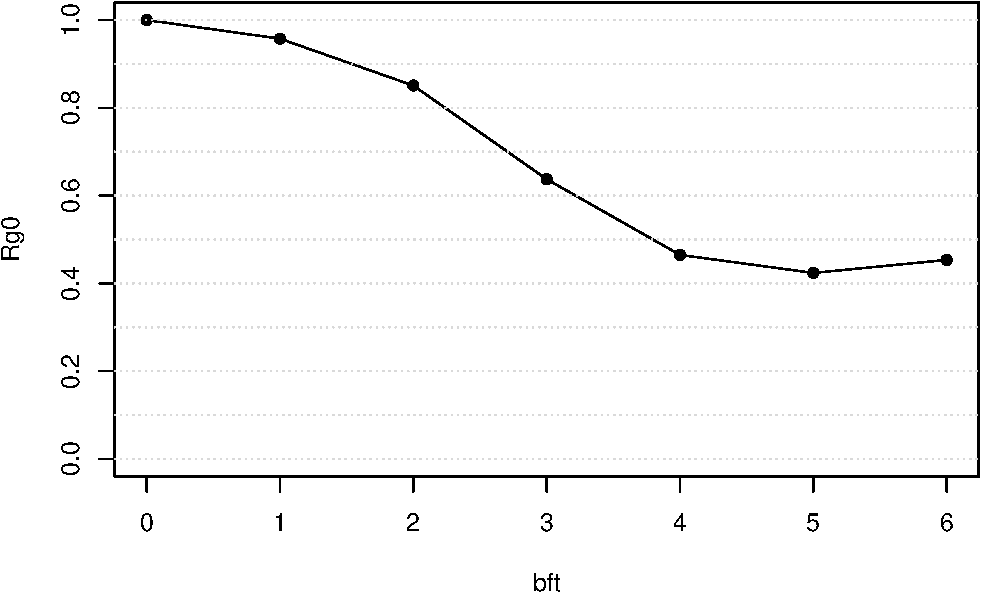
\includegraphics{figures/unnamed-chunk-202-1.pdf}

In addition to the summary above, this function returns various details, including the details of the Generalized Additive Model (GAM) (for both the estimate and the jackknifed datasets), and the raw sightings and segments used in the model.

\begin{verbatim}
[1] "Rg0"       "gam"       "jackknife" "summary"   "sightings" "segments" 
\end{verbatim}

To produce these estimates efficiently for many species, you can use the wrapper function \texttt{g0\_table()}, as follows. First you build a list of parameters for each species/species group:

\begin{Shaded}
\begin{Highlighting}[]
\NormalTok{species }\OtherTok{\textless{}{-}} \FunctionTok{list}\NormalTok{(}
  \FunctionTok{list}\NormalTok{(}\AttributeTok{spp =} \FunctionTok{c}\NormalTok{(}\StringTok{\textquotesingle{}005\textquotesingle{}}\NormalTok{, }\StringTok{\textquotesingle{}016\textquotesingle{}}\NormalTok{, }\StringTok{\textquotesingle{}017\textquotesingle{}}\NormalTok{),}
       \AttributeTok{title =} \StringTok{\textquotesingle{}Delphinus spp\textquotesingle{}}\NormalTok{,}
       \AttributeTok{truncation =} \FloatTok{5.5}\NormalTok{),}
  \FunctionTok{list}\NormalTok{(}\AttributeTok{spp =} \StringTok{\textquotesingle{}021\textquotesingle{}}\NormalTok{,}
       \AttributeTok{title =} \StringTok{"Risso\textquotesingle{}s dolphin"}\NormalTok{,}
       \AttributeTok{truncation =} \FloatTok{5.5}\NormalTok{, }
       \AttributeTok{pool\_bft =} \StringTok{\textquotesingle{}12\textquotesingle{}}\NormalTok{),}
  \FunctionTok{list}\NormalTok{(}\AttributeTok{spp =} \StringTok{\textquotesingle{}046\textquotesingle{}}\NormalTok{,}
       \AttributeTok{title =} \StringTok{\textquotesingle{}Sperm whale\textquotesingle{}}\NormalTok{,}
       \AttributeTok{truncation =} \FloatTok{5.5}\NormalTok{),}
  \FunctionTok{list}\NormalTok{(}\AttributeTok{spp =} \FunctionTok{c}\NormalTok{(}\StringTok{\textquotesingle{}047\textquotesingle{}}\NormalTok{, }\StringTok{\textquotesingle{}048\textquotesingle{}}\NormalTok{, }\StringTok{\textquotesingle{}080\textquotesingle{}}\NormalTok{),}
       \AttributeTok{title =} \StringTok{\textquotesingle{}Kogia spp\textquotesingle{}}\NormalTok{,}
       \AttributeTok{truncation =} \FloatTok{4.0}\NormalTok{),}
  \FunctionTok{list}\NormalTok{(}\AttributeTok{spp =} \StringTok{\textquotesingle{}061\textquotesingle{}}\NormalTok{,}
       \AttributeTok{title =} \StringTok{"Cuvier\textquotesingle{}s beaked whale"}\NormalTok{,}
       \AttributeTok{truncation =} \FloatTok{4.0}\NormalTok{),}
  \FunctionTok{list}\NormalTok{(}\AttributeTok{spp =} \StringTok{\textquotesingle{}074\textquotesingle{}}\NormalTok{,}
       \AttributeTok{title =} \StringTok{\textquotesingle{}Fin whale\textquotesingle{}}\NormalTok{,}
       \AttributeTok{truncation =} \FloatTok{5.5}\NormalTok{,}
       \AttributeTok{regions =} \StringTok{\textquotesingle{}CCS\textquotesingle{}}\NormalTok{))}
\end{Highlighting}
\end{Shaded}

\begin{itemize}
\item
  Note that we used shorter truncation distances for cryptic species.
\item
  Note also that we had to pool Beaufort sea states 0-2 for Risso's dolphins in order to maintain a monotonic decline in the \emph{Rg(0)} \textasciitilde{} Beaufort curve.
\item
  Note also that we limited the geostrata used to model the fin whale \emph{Rg(0)} curve to the California Current System (`CCS', after Barlow 2015), so that zero-inflated segments did not confound the model.
\end{itemize}

We then pass this species list to \texttt{g0\_table()}. In this example, we are only estimating the \emph{Rg(0)} relationship, without conducting jackknife estimation:

\begin{Shaded}
\begin{Highlighting}[]
\NormalTok{rg0s }\OtherTok{\textless{}{-}} \FunctionTok{g0\_table}\NormalTok{(cruzi,}
\NormalTok{               species,}
               \AttributeTok{eff\_types =} \StringTok{\textquotesingle{}S\textquotesingle{}}\NormalTok{,}
               \AttributeTok{jackknife\_fraction =} \ConstantTok{NULL}\NormalTok{)}
\end{Highlighting}
\end{Shaded}

Now plot the result using a dedicated \texttt{LTabundR} function:

\begin{Shaded}
\begin{Highlighting}[]
\FunctionTok{g0\_plot}\NormalTok{(rg0s, }\AttributeTok{panes=}\DecValTok{1}\NormalTok{)}
\end{Highlighting}
\end{Shaded}

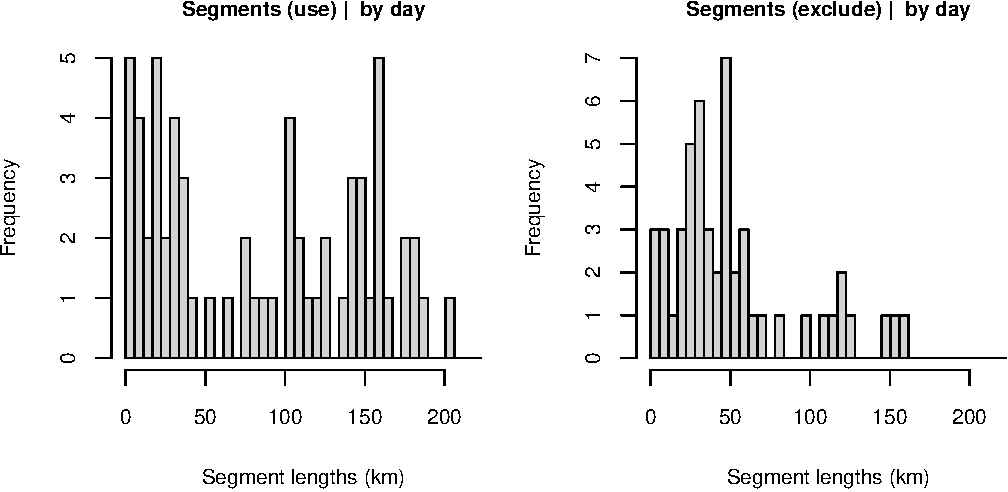
\includegraphics{figures/unnamed-chunk-208-1.pdf}

\hypertarget{weighted-average-g0}{%
\section*{\texorpdfstring{Weighted average \texttt{g(0)}}{Weighted average g(0)}}\label{weighted-average-g0}}
\addcontentsline{toc}{section}{Weighted average \texttt{g(0)}}

Since \texttt{g(0)} clearly depends upon survey conditions, and since each survey is carried out in a specific sequence of conditions, a unique, weighted \texttt{g(0)} value must be estimated for each species in each geostratum and year of interest.

This will be done automatically by the line-transect analysis functions coming up (see \texttt{LTabundR::lta()}), meaning you only need a table of \emph{Rg(0)} values in order to proceed to the next step. But you can also calculate weighted \emph{g(0)} values separately as an isolated analysis, which we show below.

Let's say we want to estimate the average \texttt{g(0)} for striped dolphins during the WHICEAS survey years of 2017 and 2020. From above, we have an estimate of the \emph{Rg(0)} and its CV for each Beaufort state:

\begin{Shaded}
\begin{Highlighting}[]
\NormalTok{rg0}\SpecialCharTok{$}\NormalTok{summary }\SpecialCharTok{\%\textgreater{}\%} \FunctionTok{select}\NormalTok{(bft, Rg0, Rg0\_CV)}
\NormalTok{  bft       Rg0    Rg0\_CV}
\DecValTok{1}   \DecValTok{0} \FloatTok{1.0000000} \FloatTok{0.0000000}
\DecValTok{2}   \DecValTok{1} \FloatTok{0.9574903} \FloatTok{0.1090064}
\DecValTok{3}   \DecValTok{2} \FloatTok{0.8507491} \FloatTok{0.1889574}
\DecValTok{4}   \DecValTok{3} \FloatTok{0.6374127} \FloatTok{0.2048128}
\DecValTok{5}   \DecValTok{4} \FloatTok{0.4649322} \FloatTok{0.1829984}
\DecValTok{6}   \DecValTok{5} \FloatTok{0.4238391} \FloatTok{0.1854241}
\DecValTok{7}   \DecValTok{6} \FloatTok{0.4534225} \FloatTok{0.2244517}
\end{Highlighting}
\end{Shaded}

We also have a processed \texttt{cruz} object with 2017 data:

\begin{Shaded}
\begin{Highlighting}[]
\FunctionTok{load}\NormalTok{(}\StringTok{\textquotesingle{}whiceas\_cruz\_1720.RData\textquotesingle{}}\NormalTok{)}
\NormalTok{cruz\_17 }\OtherTok{\textless{}{-}} \FunctionTok{filter\_cruz}\NormalTok{(cruz\_1720, }\AttributeTok{years =} \DecValTok{2017}\NormalTok{, }\AttributeTok{verbose=}\ConstantTok{FALSE}\NormalTok{)}
\end{Highlighting}
\end{Shaded}

To view the distribution of effort in this WHICEAS 2017 across sea states, we can use the function \texttt{summarize\_bft()}:

\begin{Shaded}
\begin{Highlighting}[]
\FunctionTok{summarize\_bft}\NormalTok{(cruz\_17)}\SpecialCharTok{$}\NormalTok{overall}
\CommentTok{\# A tibble: 6 x 3}
\NormalTok{   bftr    km   prop}
  \SpecialCharTok{\textless{}}\NormalTok{dbl}\SpecialCharTok{\textgreater{}} \ErrorTok{\textless{}}\NormalTok{dbl}\SpecialCharTok{\textgreater{}}  \ErrorTok{\textless{}}\NormalTok{dbl}\SpecialCharTok{\textgreater{}}
\DecValTok{1}     \DecValTok{1}  \FloatTok{130.} \FloatTok{0.0200}
\DecValTok{2}     \DecValTok{2}  \FloatTok{583.} \FloatTok{0.0897}
\DecValTok{3}     \DecValTok{3}  \FloatTok{901.} \FloatTok{0.139} 
\DecValTok{4}     \DecValTok{4} \FloatTok{2140.} \FloatTok{0.329} 
\DecValTok{5}     \DecValTok{5} \FloatTok{1873.} \FloatTok{0.288} 
\DecValTok{6}     \DecValTok{6}  \FloatTok{875.} \FloatTok{0.135} 
\end{Highlighting}
\end{Shaded}

We then use the function \texttt{g0\_weighted\_var()} to compute the weighted \emph{Rg(0)} for our survey as well as its CV. This function carries out an automated optimization routine to simulate a new distribution for the weighted \emph{g(0)}, which is then used to estimate the weighted CV.

\begin{Shaded}
\begin{Highlighting}[]
\NormalTok{weighted\_g0\_2017 }\OtherTok{\textless{}{-}} 
  \FunctionTok{g0\_weighted}\NormalTok{(}\AttributeTok{Rg0 =}\NormalTok{ rg0}\SpecialCharTok{$}\NormalTok{summary}\SpecialCharTok{$}\NormalTok{Rg0,}
              \AttributeTok{Rg0\_cv =}\NormalTok{ rg0}\SpecialCharTok{$}\NormalTok{summary}\SpecialCharTok{$}\NormalTok{Rg0\_CV, }
              \AttributeTok{cruz =}\NormalTok{ cruz\_17)}
\end{Highlighting}
\end{Shaded}

The result:

\begin{Shaded}
\begin{Highlighting}[]
\NormalTok{weighted\_g0\_2017}\SpecialCharTok{$}\NormalTok{g0[}\DecValTok{1}\SpecialCharTok{:}\DecValTok{2}\NormalTok{]}
\NormalTok{  wt.mean wt.cv}
\DecValTok{1}   \FloatTok{0.526} \FloatTok{0.188}
\end{Highlighting}
\end{Shaded}

Now let's do the same for WHICEAS 2020 and compare the weighted \emph{g(0)} estimate:

\begin{Shaded}
\begin{Highlighting}[]
\CommentTok{\# Filter to 2020}
\NormalTok{cruz\_20 }\OtherTok{\textless{}{-}} \FunctionTok{filter\_cruz}\NormalTok{(cruz\_1720, }\AttributeTok{years =} \DecValTok{2020}\NormalTok{, }\AttributeTok{verbose=}\ConstantTok{FALSE}\NormalTok{)}

\CommentTok{\# Summarize Bft effort}
\FunctionTok{summarize\_bft}\NormalTok{(cruz\_20)}\SpecialCharTok{$}\NormalTok{overall}
\CommentTok{\# A tibble: 6 x 3}
\NormalTok{   bftr     km   prop}
  \SpecialCharTok{\textless{}}\NormalTok{dbl}\SpecialCharTok{\textgreater{}}  \ErrorTok{\textless{}}\NormalTok{dbl}\SpecialCharTok{\textgreater{}}  \ErrorTok{\textless{}}\NormalTok{dbl}\SpecialCharTok{\textgreater{}}
\DecValTok{1}     \DecValTok{1}   \FloatTok{88.2} \FloatTok{0.0165}
\DecValTok{2}     \DecValTok{2}  \FloatTok{262.}  \FloatTok{0.0490}
\DecValTok{3}     \DecValTok{3}  \FloatTok{434.}  \FloatTok{0.0813}
\DecValTok{4}     \DecValTok{4} \FloatTok{1482.}  \FloatTok{0.278} 
\DecValTok{5}     \DecValTok{5} \FloatTok{2004.}  \FloatTok{0.376} 
\DecValTok{6}     \DecValTok{6} \FloatTok{1067.}  \FloatTok{0.200} 
\end{Highlighting}
\end{Shaded}

Note that conditions were a bit worse in 2020 compared to 2017. We therefore expect the weighted \emph{g(0)} estimate to be lower:

\begin{Shaded}
\begin{Highlighting}[]
\NormalTok{weighted\_g0\_2020 }\OtherTok{\textless{}{-}} 
  \FunctionTok{g0\_weighted}\NormalTok{(}\AttributeTok{Rg0 =}\NormalTok{ rg0}\SpecialCharTok{$}\NormalTok{summary}\SpecialCharTok{$}\NormalTok{Rg0,}
              \AttributeTok{Rg0\_cv =}\NormalTok{ rg0}\SpecialCharTok{$}\NormalTok{summary}\SpecialCharTok{$}\NormalTok{Rg0\_CV, }
              \AttributeTok{cruz =}\NormalTok{ cruz\_20)}
\end{Highlighting}
\end{Shaded}

The result:

\begin{Shaded}
\begin{Highlighting}[]
\NormalTok{weighted\_g0\_2020}\SpecialCharTok{$}\NormalTok{g0[}\DecValTok{1}\SpecialCharTok{:}\DecValTok{2}\NormalTok{]}
\NormalTok{  wt.mean wt.cv}
\DecValTok{1}   \FloatTok{0.494}  \FloatTok{0.19}
\end{Highlighting}
\end{Shaded}

Confirmed: weighted \emph{g(0)} for 2020 is slightly lower than in 2017, due to generally worse survey conditions. These year-specific estimates should prevent those different conditions from impacting their respective abundance estimates.

\hypertarget{lta}{%
\chapter{Line-transect analysis}\label{lta}}

We use line-transect analysis to produce estimates of animal density and/or abundance based upon surveys. The main \texttt{LTabundR} function for conducting line-transect analysis is \texttt{lta()}, which calls for four primary arguments in addition to your \texttt{cruz} object:

\begin{Shaded}
\begin{Highlighting}[]
\FunctionTok{lta}\NormalTok{(cruz,}
\NormalTok{    Rg0,}
\NormalTok{    fit\_filters,}
\NormalTok{    df\_settings,}
\NormalTok{    estimates)}
\end{Highlighting}
\end{Shaded}

Below we explain each of these inputs, discuss other optional inputs, and explore the results produced by \texttt{lta()}.

\hypertarget{key-inputs}{%
\section*{Key inputs}\label{key-inputs}}
\addcontentsline{toc}{section}{Key inputs}

\hypertarget{cruz}{%
\subsection*{\texorpdfstring{\texttt{cruz}}{cruz}}\label{cruz}}
\addcontentsline{toc}{subsection}{\texttt{cruz}}

This is the \texttt{cruz} object you have generated with \texttt{process\_surveys()}. Before running \texttt{lta()}, ensure that this \texttt{cruz} object is filtered only to the years, regions, and sighting conditions you would like to use for detection function fitting. Filter your cruz object with full flexibility using \texttt{LTabundR::filter\_cruz()}. Note that filtering for detection function fitting is typically less stringent than filtering for downstream steps for abundance estimation, since as many sightings are included as possible to combat low sample sizes, as long as sightings were observed using standard methods in an unbiased search pattern, and as long as you do not expect detectability to vary across years and regions.

Here we will work with a version of the 1986-2020 Central North Pacific survey data we processed a few pages back. This version is included as a built-in dataset within \texttt{LTabundR}:

\begin{Shaded}
\begin{Highlighting}[]
\FunctionTok{load}\NormalTok{(}\StringTok{\textquotesingle{}whiceas\_cruz.RData\textquotesingle{}}\NormalTok{)}
\end{Highlighting}
\end{Shaded}

As it is provided, this dataset does not need any filtering.

We will use these data to estimate the abundance of striped dolphins (\emph{Stenella coeruleoalba}), Fraser's dolphins (\emph{Lagenodelphis hosei}), and Melon-headed whales (\emph{Preponocephala electra}) within the WHICEAS study area in 2017 and 2020. We will group these three species into a `species pool' in order to gain a sufficient sample size for fitting a detection function. We will then use ``Species'' as a covariate within the detection function model, along with other variables including Beaufort Sea State, ship name, and log-transformed school size.

\hypertarget{rg0}{%
\subsection*{\texorpdfstring{\texttt{Rg0}}{Rg0}}\label{rg0}}
\addcontentsline{toc}{subsection}{\texttt{Rg0}}

The result of \texttt{LTabundR::g0\_model()}, which is a \texttt{data.frame} with Relative trackline detection probabilities, \emph{Rg(0)}, for each species in each Beaufort sea state. See \texttt{LTabundR} dataset \texttt{data("g0\_results")}, used below, as an example.

This is an \emph{optional} input. If not provided, \emph{g(0)} will be assumed to 1.0, and its CV will be assumed to be 0. Alternatively, you can manually specify values for \emph{g(0)} and its CV in the \texttt{estimates} argument below.

Here we will use a \texttt{data.frame} of \emph{Rg(0)} estimates based on the same survey years, 1986 - 2020, which has been provided as a built-in dataset:

\begin{Shaded}
\begin{Highlighting}[]
\FunctionTok{data}\NormalTok{(}\StringTok{"g0\_results"}\NormalTok{)}
\NormalTok{Rg0 }\OtherTok{\textless{}{-}}\NormalTok{ g0\_results}
\end{Highlighting}
\end{Shaded}

\hypertarget{fit_filters}{%
\subsection*{\texorpdfstring{\texttt{fit\_filters}}{fit\_filters}}\label{fit_filters}}
\addcontentsline{toc}{subsection}{\texttt{fit\_filters}}

The \texttt{fit\_filters} input specifies how to filter the data before fitting the detection function. It accepts a named list, which in our example will look like this:

\begin{Shaded}
\begin{Highlighting}[]
\NormalTok{fit\_filters }\OtherTok{=} \FunctionTok{list}\NormalTok{(}\AttributeTok{spp =} \FunctionTok{c}\NormalTok{(}\StringTok{\textquotesingle{}013\textquotesingle{}}\NormalTok{, }\StringTok{\textquotesingle{}026\textquotesingle{}}\NormalTok{, }\StringTok{\textquotesingle{}031\textquotesingle{}}\NormalTok{), }
                   \AttributeTok{pool =} \StringTok{\textquotesingle{}Multi{-}species pool 1\textquotesingle{}}\NormalTok{,}
                   \AttributeTok{cohort =} \StringTok{\textquotesingle{}all\textquotesingle{}}\NormalTok{,}
                   \AttributeTok{truncation\_distance =} \DecValTok{5}\NormalTok{,}
                   \AttributeTok{other\_species =} \StringTok{\textquotesingle{}remove\textquotesingle{}}\NormalTok{)}
\end{Highlighting}
\end{Shaded}

\begin{itemize}
\item
  \textbf{\texttt{spp}}: A character vector of species codes. Using multiple species codes may be useful when you have low sample sizes for a cohort of similar species.
\item
  \textbf{\texttt{cohort}}: The cohort containing these species, provided as a name or a number indicating which slot in \texttt{cruz\$cohorts} should be referenced.
\item
  \textbf{\texttt{truncation\_distance}}: The truncation distance to apply during model fitting.
\end{itemize}

\emph{The remaining inputs are optional (i.e., they all have defaults):}

\begin{itemize}
\item
  \textbf{\texttt{pool}}: A character string, providing a title for this species pool. If not specified, the species codes used will be concatenated to produce a title automatically.
\item
  \textbf{\texttt{other\_species}}: A character vector with four recognized values:

  \begin{itemize}
  \tightlist
  \item
    If \texttt{"apply"} (the default if not specified), the species code will be changed to \texttt{"Other"} for sightings in which the species was in a mixed-species school but was not the species with the largest percentage of the total school size. In those cases, the species was not as relevant to the detection of the school as the other species were, which may bias the detection function. This creates a factor level for the detection function to use (when \texttt{"species"} is a covariate) to distinguish between cue-relevant species that are within the specified pool and those that are not.
  \item
    The second option for \texttt{other\_species} is \texttt{"ignore"}, which does \textbf{not} reassign species codes to \texttt{"Other"}, and ignores whether the species of interest held the plurality for a mixed species detection.
  \item
    The third option is \texttt{"remove"}: any species re-assigned to \texttt{"Other"} will be removed before the detection function is fit; this can be useful if only a small number of species are re-assigned to \texttt{"Other"}, which would then obviate \texttt{species} as a viable covariate (since the sample size of all \texttt{species} levels would be unlikely to exceed \texttt{df\_settings\$covariates\_n\_per\_level} -- see below).
  \item
    The fourth and final option is \texttt{coerce}, which forces \emph{all} species codes to \texttt{"Other"} for the purposes of detection function fitting and abundance estimation. This is effectively the same as removing `species' from the list of covariates, but this option can be a convenience if you want to quickly toggle the use of \texttt{species} as a covariate for a specific species pool, and/or produce abundance estimates for unidentified taxa (e.g., an `Unidentified dolphins' species pool that includes multiple species codes).
  \end{itemize}
\end{itemize}

~

\hypertarget{df_settings}{%
\subsection*{\texorpdfstring{\texttt{df\_settings}}{df\_settings}}\label{df_settings}}
\addcontentsline{toc}{subsection}{\texttt{df\_settings}}

The \texttt{df\_settings} input specifies how to fit a detection function to the filtered data. It accepts a named list, which in our example will look like this:

\begin{Shaded}
\begin{Highlighting}[]
\NormalTok{df\_settings }\OtherTok{=} \FunctionTok{list}\NormalTok{(}\AttributeTok{covariates =} \FunctionTok{c}\NormalTok{(}\StringTok{\textquotesingle{}bft\textquotesingle{}}\NormalTok{,}\StringTok{\textquotesingle{}lnsstot\textquotesingle{}}\NormalTok{,}\StringTok{\textquotesingle{}cruise\textquotesingle{}}\NormalTok{,}\StringTok{\textquotesingle{}year\textquotesingle{}}\NormalTok{,}\StringTok{\textquotesingle{}ship\textquotesingle{}}\NormalTok{,}\StringTok{\textquotesingle{}species\textquotesingle{}}\NormalTok{),}
                   \AttributeTok{covariates\_factor =} \FunctionTok{c}\NormalTok{(}\ConstantTok{FALSE}\NormalTok{, }\ConstantTok{FALSE}\NormalTok{, }\ConstantTok{TRUE}\NormalTok{, }\ConstantTok{TRUE}\NormalTok{, }\ConstantTok{TRUE}\NormalTok{, }\ConstantTok{TRUE}\NormalTok{),}
                   \AttributeTok{covariates\_levels =} \DecValTok{2}\NormalTok{,}
                   \AttributeTok{covariates\_n\_per\_level =} \DecValTok{10}\NormalTok{,}
                   \AttributeTok{detection\_function\_base =} \StringTok{\textquotesingle{}hn\textquotesingle{}}\NormalTok{,}
                   \AttributeTok{base\_model =} \StringTok{\textquotesingle{}\textasciitilde{}1\textquotesingle{}}\NormalTok{,}
                   \AttributeTok{delta\_aic =} \DecValTok{2}\NormalTok{)}
\end{Highlighting}
\end{Shaded}

\emph{(Note that all of these inputs have defaults, and are therefore optional.)}

\begin{itemize}
\item
  \textbf{\texttt{covariates}} Covariates you wish to include as candidates in detection function models, provided as a character vector. The covariates must match columns existing within \texttt{cruz\$cohorts\$\textless{}cohort\_name\textgreater{}\$sightings}. Note that the function will ignore case, coercing all covariates to lowercase. Default: no covariates.
\item
  \textbf{\texttt{covariates\_factor}} A Boolean vector, which must be the same length as \texttt{covariates}, indicating whether each covariate should be treated as a factor instead of a numeric. Default: \texttt{NULL}.
\item
  \textbf{\texttt{covariates\_levels}} The minimum number of levels a factor covariate must have in order to be included as an eligible covariate. Default: \texttt{2}.
\item
  \textbf{\texttt{covariates\_n\_per\_level}} The minimum number of observations within each level of a factor covariate. If this condition is not met, the covariate is excluded from the candidates. Default: \texttt{10}.
\item
  \textbf{\texttt{detection\_function\_base}} The base key for the detection function, provided as a character vector. Accepted values are \texttt{"hn"} (half-normal key, the default, which exhibits greater stability when fitting to cetacean survey data; Gerrogette and Forcada 2005), \texttt{"hr"} (hazard-rate), or \texttt{c("hn",\ "hr)}, which will loop through both keys and attempt model fitting.
\item
  \textbf{\texttt{base\_model}} The initial model formula, upon which to build using candidate covariates. If not provided by the user, the default is \texttt{"\textasciitilde{}\ 1"}.
\item
  \textbf{\texttt{delta\_aic}} The AIC difference between the model yielding the lowest AIC and other candidate models, used to define the best-fitting models. Typically, AIC differences of less than 2 (the default) indicate effectively equal model performance. If this value is not zero, then model averaging will be done: if multiple models are within \texttt{delta\_aic} of the model with the lowest AIC, all ``best'' models will be used in subsequent steps and their results will be averaged. See \texttt{Details} below.
\end{itemize}

\hypertarget{estimates}{%
\subsection*{\texorpdfstring{\texttt{estimates}}{estimates}}\label{estimates}}
\addcontentsline{toc}{subsection}{\texttt{estimates}}

The \texttt{estimates} input specifies which estimates of density and abundance to produce based on the fitted detection function. This input accepts a list of sub-lists, which in our example will look something like this:

\begin{Shaded}
\begin{Highlighting}[]
\NormalTok{estimates }\OtherTok{\textless{}{-}} \FunctionTok{list}\NormalTok{(}\FunctionTok{list}\NormalTok{(}\AttributeTok{spp =} \StringTok{\textquotesingle{}013\textquotesingle{}}\NormalTok{,}
                       \AttributeTok{title =} \StringTok{\textquotesingle{}Striped dolphin\textquotesingle{}}\NormalTok{,}
                       \AttributeTok{years =} \DecValTok{2017}\NormalTok{,}
                       \AttributeTok{regions =} \StringTok{\textquotesingle{}WHICEAS\textquotesingle{}}\NormalTok{))}
\end{Highlighting}
\end{Shaded}

This example shows only a single sub-list, specifying how to generate a density/abundance estimate for striped dolphins (species code 013) within the ``WHICEAS'' geostratum for 2017.

\begin{itemize}
\item
  \textbf{\texttt{spp}}: A character vector of species codes.
\item
  \textbf{\texttt{title}}: A title for this abundance estimate, given as a character vector, ' e.g., \texttt{"Striped\ dolphin\ -\ pelagic"}. If left blank, the species code(s) will be concatenated to use as a title.
\item
  \textbf{\texttt{years}}: A numeric vector of years, used to filter data to include only effort/sightings from these years.
\item
  \textbf{\texttt{regions}}: A character vector of geostratum names, used to filter the data. Any segment or sighting occurring within \emph{any} (but \emph{not} necessarily all) of the provided \texttt{regions} will be returned. This holds true for nested regions: for example, in analyses from the Central North Pacific, in which the Hawaii EEZ geostratum (\texttt{"HI-EEZ"}) is nested within the larger geostratum representing the entire CNP study area (\texttt{"OtherCNP"}), an input of \texttt{regions\ =\ "OtherCNP"} will return segments/sightings \emph{both} inside the Hawaii EEZ \emph{and} outside of it.
\end{itemize}

You also have the option of manually specifying other filters \& arguments. Each of these sub-lists accepts the following named slots:

\begin{itemize}
\item
  \textbf{\texttt{cruises}}: An optional numeric vector of cruise numbers, used to filter data to include effort/sighting from only certain cruises. Ignored if \texttt{NULL.}
\item
  \textbf{\texttt{regions\_remove}}: A character vector of geostratum names, similar to above. Any segment or sighting occurring within any of these \texttt{not\_regions} will \textbf{not} be returned. Using the example above, if \texttt{regions\ =\ "OtherCNP"} and \texttt{not\_regions\ =\ "HI-EEZ"}, only segments occuring within \texttt{OtherCNP} \emph{and} outside of \texttt{HI-EEZ} will be returned. This can be particularly useful for abundance estimates for pelagic stock that exclude nested insular stocks.
\item
  \textbf{\texttt{g0}}: If left as the default \texttt{NULL}, the \texttt{lta()} function will automatically estimate the weighted trackline detection probability \emph{(g0)} according to the distribution of Beaufort sea states contained within the survey years/regions for which density/abundance is being estimated (this is done using the \texttt{LTabundR} function \texttt{g0\_weighted()}). This will only be done if the \texttt{Rg0} input above is not \texttt{NULL}; if it is and you do not provide \emph{g(0)} values here, \texttt{g0} will be coerced to equal 1. To coerce \texttt{g(0)} to a certain value of your own choosing, you can provide a numeric vector of length 1 or 2. If length 1, this value represents \emph{g(0)} for all schools regardless of size. If length 2, these values represent \emph{g(0)} for small and large school sizes, as defined by \texttt{g0\_threshold} below.
\item
  \textbf{\texttt{g0\_cv}}: Similar to g0 above: if left \texttt{NULL}, the CV of the \texttt{g(0)} estimate will be automatically estimated based on weighted survey conditions. Alternatively, you can manually specify a CV here, using a numeric vector of length 1 or 2. If you do not specify a value and \texttt{Rg0} input is NULL, \texttt{g0\_cv} will be coerced to equal 0.
\item
  \textbf{\texttt{g0\_threshold}}: The school size threshold between small and large groups.
\item
  \textbf{\texttt{alt\_g0\_spp}}: An alternate species code to use to draw Relative \emph{g(0)} values from the \texttt{Rg0} input. This is useful in the event that \emph{Rg(0)} was not estimated for the species whose density/abundance you are estimating, but there is a similarly detectable species whose \emph{Rg(0)} parameters have been estimated.
\item
  \textbf{\texttt{combine\_g0}}: A Boolean, with default \texttt{FALSE}. If \texttt{TRUE}, weighted \emph{g0} estimates will be produced separately for each species code provided (specifically, for each unique row in the \texttt{Rg0} table that is found after filtering by the species codes you provide in this estimate), \emph{THEN} average those estimates together. This can be useful when you do not have a \emph{Rg(0)} estimates for a certain species, but you can approximate \emph{g0} by averaging together estimates from multiple species (e.g., averaging together weighted \emph{g(0)} from across rorqual species in order to get a weighted \emph{g(0)} estimate for `Unidentified rorquals').
\item
  \textbf{\texttt{region\_title}}: An optional character vector indicating the title you would like to give to the region pertaining to this estimate. This can be useful if you have a complicated assemblage of regions you are combining and/or removing. If not supplied, the function will automatically generate a \texttt{region\_title} based on \texttt{regions} and \texttt{regions\_remove}.
\item
  \textbf{\texttt{forced\_effort}}: If this is a single numeric value instead of \texttt{NULL} (\texttt{NULL} is the default), this value will be used as the survey effort, in km, in a brute-force method; this same value will be used for every year and region. This is only helpful if you are looking for a relatively easy way to compare results from your own analysis to another (e.g., comparing \texttt{LTabundR} results to reports from NOAA reports prior to 2021, in which effort was calculated slightly differently).
\item
  \textbf{\texttt{area}}: If this is a single numeric value instead of \texttt{NULL} (\texttt{NULL} is the default), this value will be used as the area of the region in which abundance is being estimated, in square km, in a brute-force approach. If left \texttt{NULL}, the function will calculate the final area of the survey area resulting from the regions and regions\_remove filters above.
\item
  \textbf{\texttt{remove\_land}}: A Boolean, with default \texttt{TRUE}, indicating whether or not land area should be removed from the survey area before calculating its area for abundance estimation. This term is only referenced if area is not specified manually.
\end{itemize}

Here is the full \texttt{estimates} list for all the species-year-geostratum combinations for which we want to estimate density/abundance:

\begin{Shaded}
\begin{Highlighting}[]
\NormalTok{estimates }\OtherTok{\textless{}{-}} \FunctionTok{list}\NormalTok{(}
    \FunctionTok{list}\NormalTok{(}\AttributeTok{spp =} \StringTok{\textquotesingle{}013\textquotesingle{}}\NormalTok{,}
         \AttributeTok{title =} \StringTok{\textquotesingle{}Striped dolphin\textquotesingle{}}\NormalTok{,}
         \AttributeTok{years =} \DecValTok{2017}\NormalTok{,}
         \AttributeTok{regions =} \StringTok{\textquotesingle{}WHICEAS\textquotesingle{}}\NormalTok{),}
    \FunctionTok{list}\NormalTok{(}\AttributeTok{spp =} \StringTok{\textquotesingle{}013\textquotesingle{}}\NormalTok{,}
         \AttributeTok{title =} \StringTok{\textquotesingle{}Striped dolphin\textquotesingle{}}\NormalTok{,}
         \AttributeTok{years =} \DecValTok{2020}\NormalTok{,}
         \AttributeTok{regions =} \StringTok{\textquotesingle{}WHICEAS\textquotesingle{}}\NormalTok{),}
    \FunctionTok{list}\NormalTok{(}\AttributeTok{spp =} \StringTok{\textquotesingle{}026\textquotesingle{}}\NormalTok{,}
         \AttributeTok{title =} \StringTok{\textquotesingle{}Frasers dolphin\textquotesingle{}}\NormalTok{,}
         \AttributeTok{years =} \DecValTok{2017}\NormalTok{,}
         \AttributeTok{regions =} \StringTok{\textquotesingle{}WHICEAS\textquotesingle{}}\NormalTok{),}
    \FunctionTok{list}\NormalTok{(}\AttributeTok{spp =} \StringTok{\textquotesingle{}026\textquotesingle{}}\NormalTok{,}
         \AttributeTok{title =} \StringTok{\textquotesingle{}Frasers dolphin\textquotesingle{}}\NormalTok{,}
         \AttributeTok{years =} \DecValTok{2020}\NormalTok{,}
         \AttributeTok{regions =} \StringTok{\textquotesingle{}WHICEAS\textquotesingle{}}\NormalTok{),}
    \FunctionTok{list}\NormalTok{(}\AttributeTok{spp =} \StringTok{\textquotesingle{}031\textquotesingle{}}\NormalTok{,}
         \AttributeTok{title =} \StringTok{\textquotesingle{}Melon{-}headed whale\textquotesingle{}}\NormalTok{,}
         \AttributeTok{years =} \DecValTok{2017}\NormalTok{,}
         \AttributeTok{regions =} \StringTok{\textquotesingle{}WHICEAS\textquotesingle{}}\NormalTok{),}
    \FunctionTok{list}\NormalTok{(}\AttributeTok{spp =} \StringTok{\textquotesingle{}031\textquotesingle{}}\NormalTok{,}
         \AttributeTok{title =} \StringTok{\textquotesingle{}Melon{-}headed whale\textquotesingle{}}\NormalTok{,}
         \AttributeTok{years =} \DecValTok{2020}\NormalTok{,}
         \AttributeTok{regions =} \StringTok{\textquotesingle{}WHICEAS\textquotesingle{}}\NormalTok{))}
\end{Highlighting}
\end{Shaded}

Each of these sub-lists specifies the details for a single estimate of density/abundance, making it possible to produce multiple estimates from the same detection function model. Generally, there needs to be a sub-list for each species-region-year combination of interest.

You can imagine that building up these sub-lists can get tedious. It can also introduce the possibility of error or inconsistencies across estimates of multiple species. To address that issue, \texttt{LTabundR} includes the function \texttt{lta\_estimates()}, which makes your code for preparing an \texttt{estimates} object much more efficient. That function is demonstrated in the Case Studies chapters.

Quickly review results:

\begin{Shaded}
\begin{Highlighting}[]
\NormalTok{results}\SpecialCharTok{$}\NormalTok{estimate}
\NormalTok{               title species    Region     Area year segments       km}
\DecValTok{1}\NormalTok{    Striped dolphin     }\DecValTok{013}\NormalTok{ (WHICEAS) }\FloatTok{402948.7} \DecValTok{2017}       \DecValTok{29} \FloatTok{3040.009}
\DecValTok{2}\NormalTok{    Striped dolphin     }\DecValTok{013}\NormalTok{ (WHICEAS) }\FloatTok{402948.7} \DecValTok{2020}       \DecValTok{34} \FloatTok{4585.386}
\DecValTok{3}\NormalTok{    Frasers dolphin     }\DecValTok{026}\NormalTok{ (WHICEAS) }\FloatTok{402948.7} \DecValTok{2017}       \DecValTok{29} \FloatTok{3040.009}
\DecValTok{4}\NormalTok{    Frasers dolphin     }\DecValTok{026}\NormalTok{ (WHICEAS) }\FloatTok{402948.7} \DecValTok{2020}       \DecValTok{34} \FloatTok{4585.386}
\DecValTok{5}\NormalTok{ Melon}\SpecialCharTok{{-}}\NormalTok{headed whale     }\DecValTok{031}\NormalTok{ (WHICEAS) }\FloatTok{402948.7} \DecValTok{2017}       \DecValTok{29} \FloatTok{3040.009}
\DecValTok{6}\NormalTok{ Melon}\SpecialCharTok{{-}}\NormalTok{headed whale     }\DecValTok{031}\NormalTok{ (WHICEAS) }\FloatTok{402948.7} \DecValTok{2020}       \DecValTok{34} \FloatTok{4585.386}
\NormalTok{  Area\_covered ESW\_mean n g0\_est  ER\_clusters   D\_clusters N\_clusters size\_mean}
\DecValTok{1}    \FloatTok{11003.442} \FloatTok{3.619543} \DecValTok{3}  \FloatTok{0.388} \FloatTok{0.0009868393} \FloatTok{0.0003538356}  \FloatTok{142.57760}  \FloatTok{31.95079}
\DecValTok{2}    \FloatTok{16960.781} \FloatTok{3.698878} \DecValTok{3}  \FloatTok{0.364} \FloatTok{0.0006542525} \FloatTok{0.0002447343}   \FloatTok{98.61536}  \FloatTok{53.95865}
\DecValTok{3}           \ConstantTok{NA}       \ConstantTok{NA} \DecValTok{0}  \FloatTok{0.341} \FloatTok{0.0000000000} \FloatTok{0.0000000000}    \FloatTok{0.00000}        \ConstantTok{NA}
\DecValTok{4}    \FloatTok{16897.976} \FloatTok{3.685181} \DecValTok{2}  \FloatTok{0.313} \FloatTok{0.0004361683} \FloatTok{0.0001896659}   \FloatTok{76.42563} \FloatTok{132.51143}
\DecValTok{5}     \FloatTok{9538.118} \FloatTok{3.137530} \DecValTok{2}  \FloatTok{0.425} \FloatTok{0.0006578929} \FloatTok{0.0002482908}  \FloatTok{100.04846} \FloatTok{185.98103}
\DecValTok{6}    \FloatTok{15957.100} \FloatTok{3.479991} \DecValTok{3}  \FloatTok{0.393} \FloatTok{0.0006542525} \FloatTok{0.0002414466}   \FloatTok{97.29061} \FloatTok{226.13289}
\NormalTok{      size\_sd         ER          D         N}
\DecValTok{1}   \FloatTok{0.5780968} \FloatTok{0.03153029} \FloatTok{0.01131967}  \FloatTok{4561.247}
\DecValTok{2}   \FloatTok{2.7402089} \FloatTok{0.03530258} \FloatTok{0.01319739}  \FloatTok{5317.873}
\DecValTok{3}          \ConstantTok{NA} \FloatTok{0.00000000} \FloatTok{0.00000000}     \FloatTok{0.000}
\DecValTok{4} \FloatTok{182.1747087} \FloatTok{0.05779729} \FloatTok{0.02376260}  \FloatTok{9575.109}
\DecValTok{5}  \FloatTok{96.4369707} \FloatTok{0.12235559} \FloatTok{0.04481712} \FloatTok{18059.002}
\DecValTok{6} \FloatTok{175.5620746} \FloatTok{0.14794801} \FloatTok{0.05687956} \FloatTok{22919.545}
\end{Highlighting}
\end{Shaded}

More details on the \texttt{lta()} output are provided below.

\hypertarget{variance-estimation}{%
\section*{Variance estimation}\label{variance-estimation}}
\addcontentsline{toc}{section}{Variance estimation}

By default, the \texttt{lta()} function produces a single estimate of the detection function and a single estimate of density/abundance estimate for each sub-list within \texttt{estimates()}. However, you can obtain the coefficient of variation (CV) of those estimates by activating the function's bootstrap variance estimation feature. To do this, add \texttt{bootstraps} as an input specifying a large number of iterations (1,000 iterations is standard, but we suggest first testing your code with 5 - 10 bootstraps before committing; the function typically requires \textasciitilde1 hour per 100 bootstraps.).

For the purposes of example only, we will just use 10 bootstrap iterations here:

\begin{Shaded}
\begin{Highlighting}[]
\NormalTok{results }\OtherTok{\textless{}{-}} \FunctionTok{lta}\NormalTok{(cruz, Rg0,}
\NormalTok{               fit\_filters, df\_settings, estimates,}
               \AttributeTok{bootstraps =} \DecValTok{10}\NormalTok{)}
\end{Highlighting}
\end{Shaded}

This command will first produce official estimates of the detection function and density/abundance, then it will repeat the analysis for the number of iterations you have specified. In each iteration, survey segments are re-sampled according to standard bootstrap variance estimation methods (see more details below, in ``Behind the Scenes'').

\hypertarget{other-inputs}{%
\section*{Other inputs}\label{other-inputs}}
\addcontentsline{toc}{section}{Other inputs}

There are a few other optional input arguments that lend further control over the \texttt{lta()} procedure.

\begin{Shaded}
\begin{Highlighting}[]
\FunctionTok{lta}\NormalTok{(cruz,}
\NormalTok{    Rg0,}
\NormalTok{    fit\_filters,}
\NormalTok{    df\_settings,}
\NormalTok{    estimates,}
    \AttributeTok{use\_g0 =} \ConstantTok{TRUE}\NormalTok{,}
    \AttributeTok{ss\_correction =} \DecValTok{1}\NormalTok{,}
    \AttributeTok{bootstraps =} \DecValTok{10}
    \AttributeTok{toplot =} \ConstantTok{TRUE}\NormalTok{,}
    \AttributeTok{verbose =} \ConstantTok{TRUE}\NormalTok{,)}
\end{Highlighting}
\end{Shaded}

\begin{itemize}
\item
  \textbf{\texttt{use\_g0}}: A Boolean, with default \texttt{TRUE}, indicating whether or not to use custom \texttt{g(0)} value(s). If \texttt{FALSE}, the assumed \texttt{g(0)} value will be 1. This is an easy way to toggle on-and-off automated \emph{g(0)} estimation and/or ignore manually supplied \emph{g(0)} values.
\item
  \textbf{\texttt{ss\_correction}}: Should a correction be applied to school sizes? School sizes will be scaled by this number. The default, \texttt{1}, means no changes will occur.
\item
  \textbf{\texttt{toplot}}: A Boolean, with default \texttt{TRUE}, indicating whether detection function plots (\texttt{Distance::plot.ds()}) should be displayed as the candidate models are tested.
\item
  \textbf{\texttt{verbose}}: A Boolean, with default \texttt{TRUE}, indicating whether or not updates should be printed to the Console.
\end{itemize}

\hypertarget{output}{%
\section*{Output}\label{output}}
\addcontentsline{toc}{section}{Output}

\hypertarget{during-processing}{%
\subsection*{During processing}\label{during-processing}}
\addcontentsline{toc}{subsection}{During processing}

While \texttt{lta()} is running, it will print things to the Console (if \texttt{verbose} is \texttt{TRUE}), plot diagnostic plots of how the study area is being calculated (if \texttt{toplot} is \texttt{TRUE}), and plot detection function model candidates (if \texttt{toplot} is \texttt{TRUE}). To demonstrate this, we will run the estimate for striped dolphins in 2017 only, without variance bootstrapping. To expedite processing, we will manually supply \emph{g(0)} values from Bradford et al.~(2021) (this saves about 3 minutes per estimate):

\begin{Shaded}
\begin{Highlighting}[]
\NormalTok{new\_estimates }\OtherTok{\textless{}{-}} \FunctionTok{list}\NormalTok{(}
    \FunctionTok{list}\NormalTok{(}\AttributeTok{spp =} \StringTok{\textquotesingle{}013\textquotesingle{}}\NormalTok{,}
         \AttributeTok{title =} \StringTok{\textquotesingle{}Striped dolphin\textquotesingle{}}\NormalTok{,}
         \AttributeTok{years =} \DecValTok{2017}\NormalTok{,}
         \AttributeTok{regions =} \StringTok{\textquotesingle{}WHICEAS\textquotesingle{}}\NormalTok{,}
         \AttributeTok{g0 =} \FloatTok{0.35}\NormalTok{, }\AttributeTok{g0\_cv =} \FloatTok{0.19}\NormalTok{))}

\CommentTok{\# Run it:}
\NormalTok{demo }\OtherTok{\textless{}{-}} \FunctionTok{lta}\NormalTok{(cruz, Rg0, fit\_filters, df\_settings, new\_estimates)}
\end{Highlighting}
\end{Shaded}

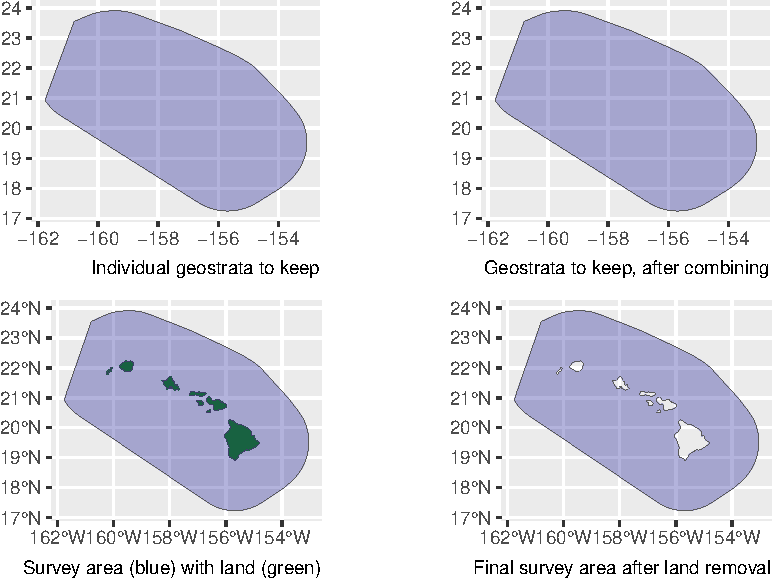
\includegraphics{figures/unnamed-chunk-237-1.pdf}

\begin{verbatim}
    Cruise            DateTime SightNoDaily line_num species Bft  lnsstot
41    1164 1988-08-08 08:05:00   19880808_9    41585     026  NA 6.856462
72    1268 1989-08-23 17:45:00  19890823_12    60352     013  NA 2.995732
82    1268 1989-11-25 06:10:00  19891125_22    66719     013  NA 4.716132
387   2001 2020-01-26 07:51:40 20200126_129   609065     013  NA 3.676782
    Cruise            DateTime SightNoDaily line_num species best ss_valid
334   1604 2016-07-07 07:15:57 20160707_105   512744   Other    1    FALSE
\end{verbatim}

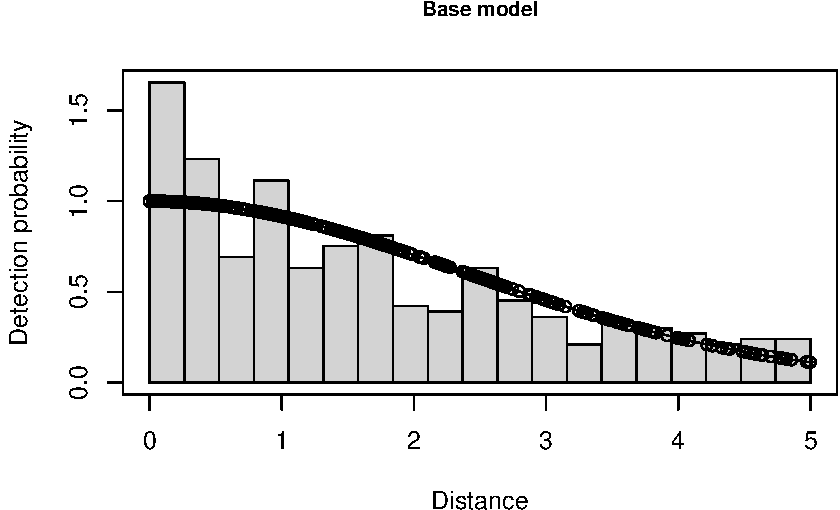
\includegraphics{figures/unnamed-chunk-237-2.pdf} 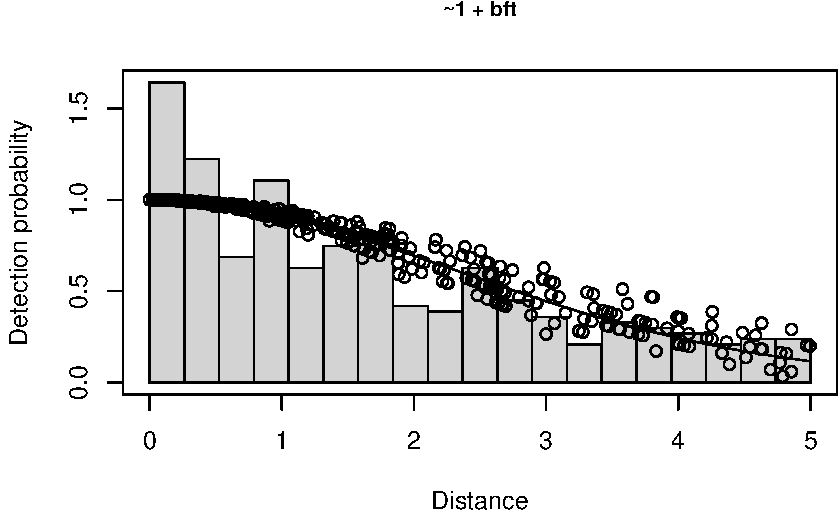
\includegraphics{figures/unnamed-chunk-237-3.pdf} 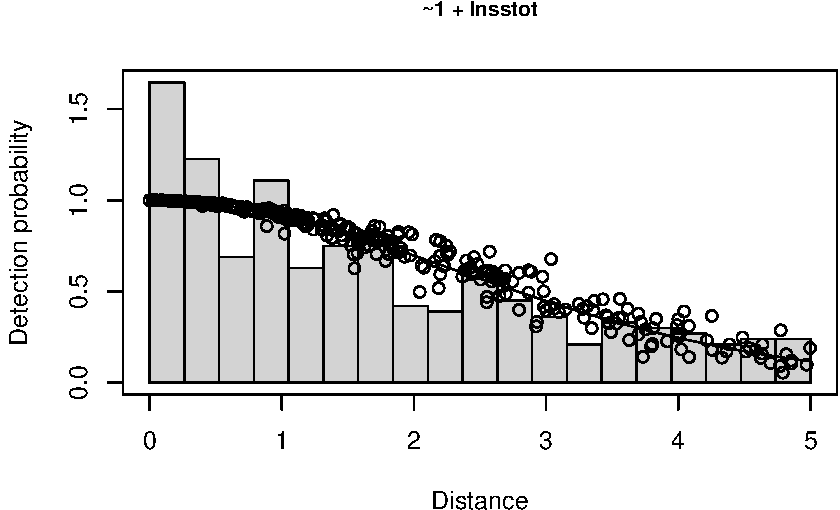
\includegraphics{figures/unnamed-chunk-237-4.pdf} 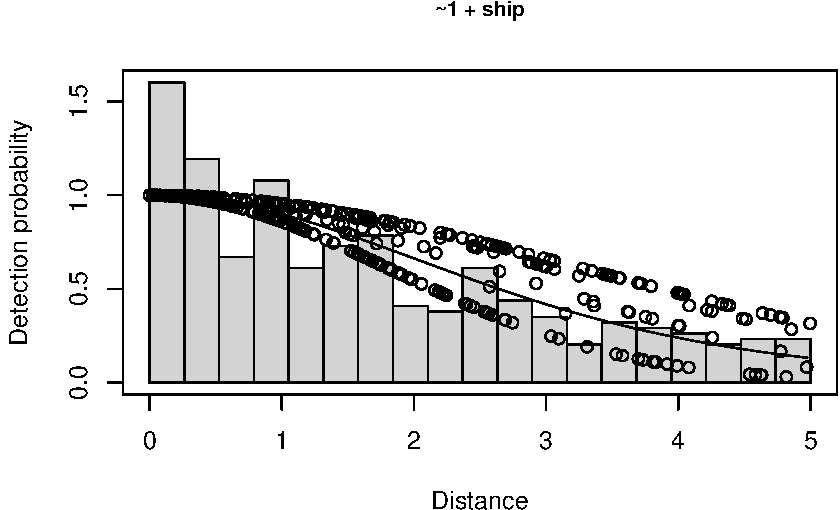
\includegraphics{figures/unnamed-chunk-237-5.pdf} 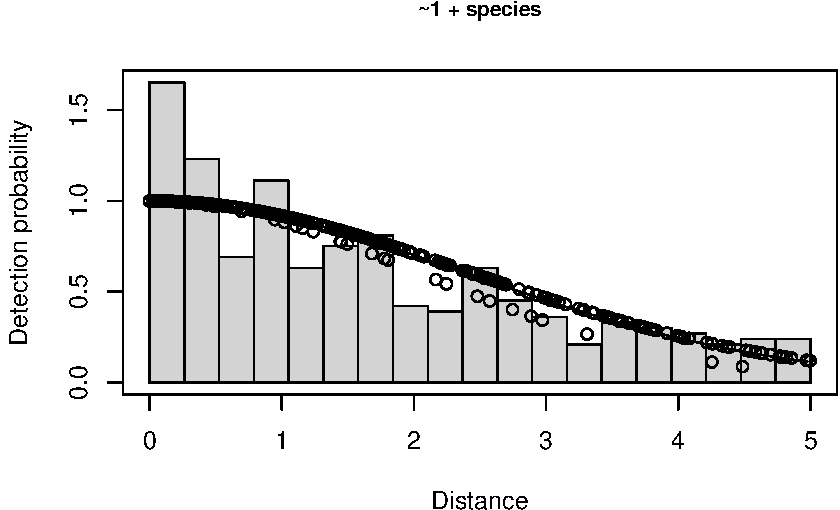
\includegraphics{figures/unnamed-chunk-237-6.pdf} 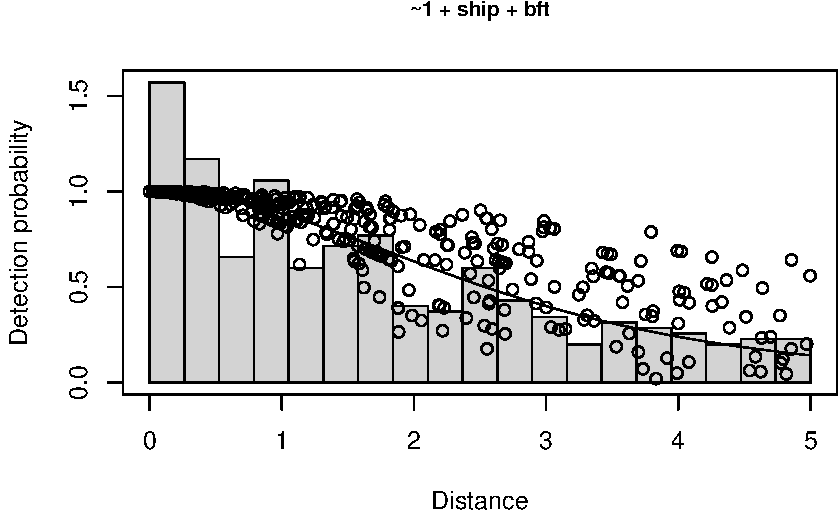
\includegraphics{figures/unnamed-chunk-237-7.pdf} 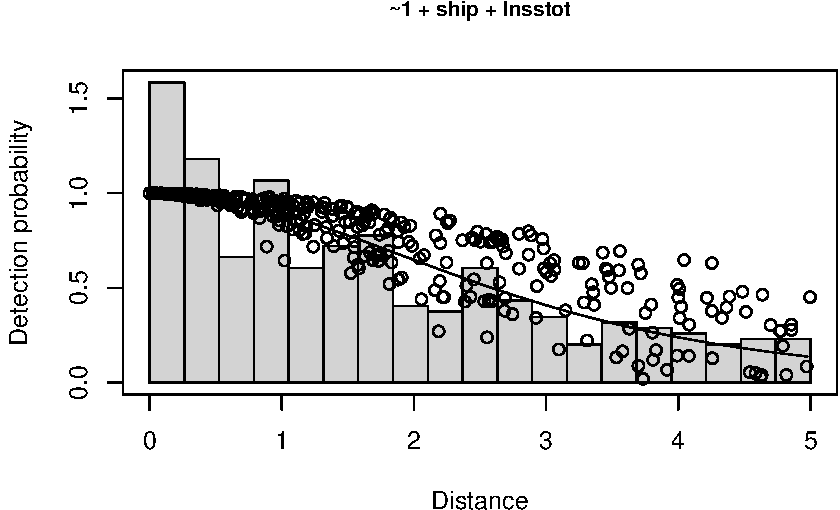
\includegraphics{figures/unnamed-chunk-237-8.pdf} 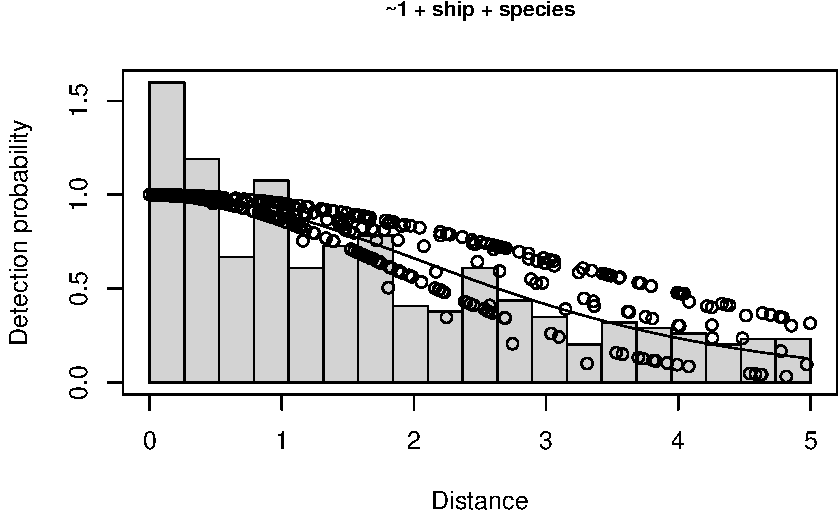
\includegraphics{figures/unnamed-chunk-237-9.pdf} 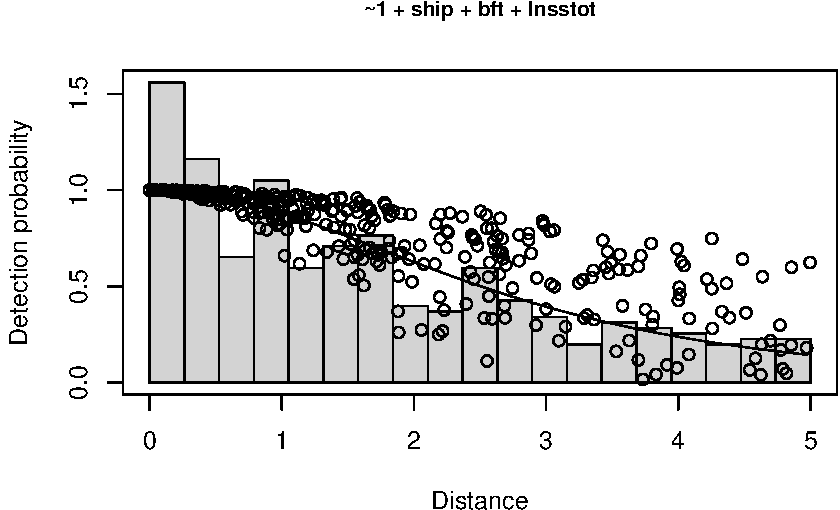
\includegraphics{figures/unnamed-chunk-237-10.pdf} 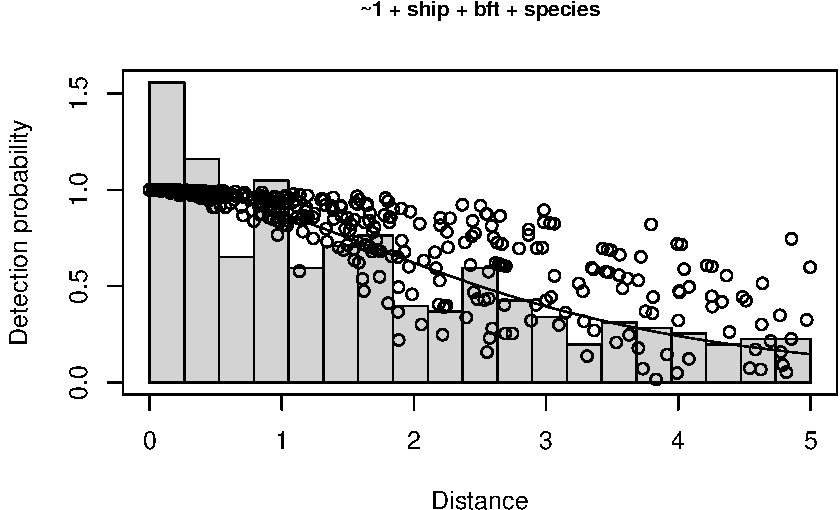
\includegraphics{figures/unnamed-chunk-237-11.pdf} 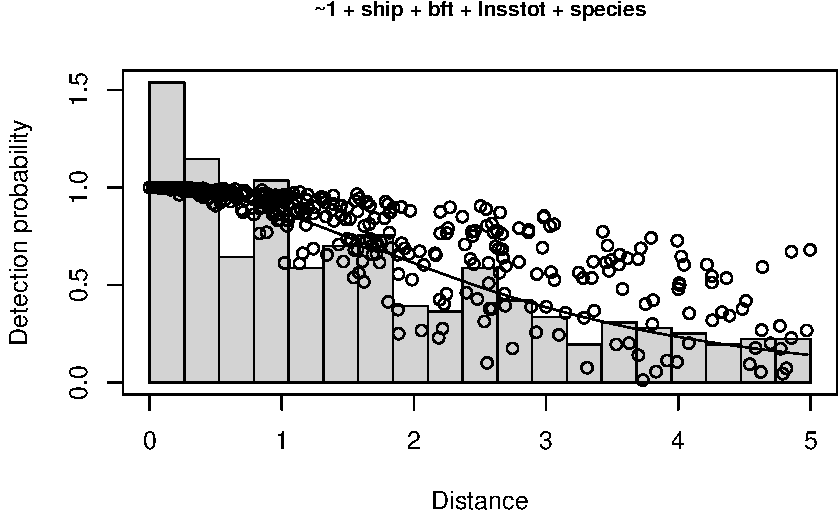
\includegraphics{figures/unnamed-chunk-237-12.pdf}

Additionally, windows will appear showing details for the detection function models and details of the density/abundance estimate.

\hypertarget{outputs}{%
\subsection*{Outputs}\label{outputs}}
\addcontentsline{toc}{subsection}{Outputs}

The \texttt{lta()} function returns a list of objects. To demonstrate this output, we will pull back in the dataset representing the result of the analysis above, for all three species in both years (with 5 bootstrap iterations):

This list of results has five slots:

\begin{Shaded}
\begin{Highlighting}[]
\FunctionTok{names}\NormalTok{(results)}
\NormalTok{[}\DecValTok{1}\NormalTok{] }\StringTok{"pool"}      \StringTok{"inputs"}    \StringTok{"estimate"}  \StringTok{"df"}        \StringTok{"bootstrap"}
\end{Highlighting}
\end{Shaded}

\begin{enumerate}
\def\labelenumi{(\arabic{enumi})}
\item
  \textbf{\texttt{pool}}: The species pool pertaining to these estimates.
\item
  \textbf{\texttt{inputs}}: A list of the inputs used to produce these estimates.
\item
  \textbf{\texttt{estimate}}: A table of density/abundance estimates for each species/region/year combination specified in the \texttt{estimates} input.
\end{enumerate}

\begin{Shaded}
\begin{Highlighting}[]
\NormalTok{results}\SpecialCharTok{$}\NormalTok{estimate}
\NormalTok{               title species    Region     Area year segments       km}
\DecValTok{1}\NormalTok{    Striped dolphin     }\DecValTok{013}\NormalTok{ (WHICEAS) }\FloatTok{402948.7} \DecValTok{2017}       \DecValTok{29} \FloatTok{3040.009}
\DecValTok{2}\NormalTok{    Striped dolphin     }\DecValTok{013}\NormalTok{ (WHICEAS) }\FloatTok{402948.7} \DecValTok{2020}       \DecValTok{34} \FloatTok{4585.386}
\DecValTok{3}\NormalTok{    Frasers dolphin     }\DecValTok{026}\NormalTok{ (WHICEAS) }\FloatTok{402948.7} \DecValTok{2017}       \DecValTok{29} \FloatTok{3040.009}
\DecValTok{4}\NormalTok{    Frasers dolphin     }\DecValTok{026}\NormalTok{ (WHICEAS) }\FloatTok{402948.7} \DecValTok{2020}       \DecValTok{34} \FloatTok{4585.386}
\DecValTok{5}\NormalTok{ Melon}\SpecialCharTok{{-}}\NormalTok{headed whale     }\DecValTok{031}\NormalTok{ (WHICEAS) }\FloatTok{402948.7} \DecValTok{2017}       \DecValTok{29} \FloatTok{3040.009}
\DecValTok{6}\NormalTok{ Melon}\SpecialCharTok{{-}}\NormalTok{headed whale     }\DecValTok{031}\NormalTok{ (WHICEAS) }\FloatTok{402948.7} \DecValTok{2020}       \DecValTok{34} \FloatTok{4585.386}
\NormalTok{  Area\_covered ESW\_mean n g0\_est  ER\_clusters   D\_clusters N\_clusters size\_mean}
\DecValTok{1}    \FloatTok{11003.442} \FloatTok{3.619543} \DecValTok{3}  \FloatTok{0.388} \FloatTok{0.0009868393} \FloatTok{0.0003538356}  \FloatTok{142.57760}  \FloatTok{31.95079}
\DecValTok{2}    \FloatTok{16960.781} \FloatTok{3.698878} \DecValTok{3}  \FloatTok{0.366} \FloatTok{0.0006542525} \FloatTok{0.0002433969}   \FloatTok{98.07648}  \FloatTok{53.95865}
\DecValTok{3}           \ConstantTok{NA}       \ConstantTok{NA} \DecValTok{0}  \FloatTok{0.345} \FloatTok{0.0000000000} \FloatTok{0.0000000000}    \FloatTok{0.00000}        \ConstantTok{NA}
\DecValTok{4}    \FloatTok{16897.976} \FloatTok{3.685181} \DecValTok{2}  \FloatTok{0.315} \FloatTok{0.0004361683} \FloatTok{0.0001884617}   \FloatTok{75.94039} \FloatTok{132.51143}
\DecValTok{5}     \FloatTok{9538.118} \FloatTok{3.137530} \DecValTok{2}  \FloatTok{0.425} \FloatTok{0.0006578929} \FloatTok{0.0002482908}  \FloatTok{100.04846} \FloatTok{185.98103}
\DecValTok{6}    \FloatTok{15957.100} \FloatTok{3.479991} \DecValTok{3}  \FloatTok{0.396} \FloatTok{0.0006542525} \FloatTok{0.0002396175}   \FloatTok{96.55356} \FloatTok{226.13289}
\NormalTok{      size\_sd         ER          D         N}
\DecValTok{1}   \FloatTok{0.5780968} \FloatTok{0.03153029} \FloatTok{0.01131967}  \FloatTok{4561.247}
\DecValTok{2}   \FloatTok{2.7402089} \FloatTok{0.03530258} \FloatTok{0.01312528}  \FloatTok{5288.814}
\DecValTok{3}          \ConstantTok{NA} \FloatTok{0.00000000} \FloatTok{0.00000000}     \FloatTok{0.000}
\DecValTok{4} \FloatTok{182.1747087} \FloatTok{0.05779729} \FloatTok{0.02361173}  \FloatTok{9514.315}
\DecValTok{5}  \FloatTok{96.4369707} \FloatTok{0.12235559} \FloatTok{0.04481712} \FloatTok{18059.002}
\DecValTok{6} \FloatTok{175.5620746} \FloatTok{0.14794801} \FloatTok{0.05644865} \FloatTok{22745.912}
\end{Highlighting}
\end{Shaded}

\begin{enumerate}
\def\labelenumi{(\arabic{enumi})}
\setcounter{enumi}{3}
\tightlist
\item
  \textbf{\texttt{df}}: A named list with details for the detection function.
\end{enumerate}

\begin{Shaded}
\begin{Highlighting}[]
\NormalTok{results}\SpecialCharTok{$}\NormalTok{df }\SpecialCharTok{\%\textgreater{}\%}\NormalTok{ names}
\NormalTok{[}\DecValTok{1}\NormalTok{] }\StringTok{"best\_models"}  \StringTok{"all\_models"}   \StringTok{"best\_objects"} \StringTok{"sightings"}    \StringTok{"sample\_size"} 
\NormalTok{[}\DecValTok{6}\NormalTok{] }\StringTok{"curve"}       

\NormalTok{results}\SpecialCharTok{$}\NormalTok{df}\SpecialCharTok{$}\NormalTok{best\_models}
\NormalTok{  Model Key\_function                             Formula     Pmean      AIC}
\DecValTok{1}    \DecValTok{11}\NormalTok{           hn }\SpecialCharTok{\textasciitilde{}}\DecValTok{1} \SpecialCharTok{+}\NormalTok{ ship }\SpecialCharTok{+}\NormalTok{ bft }\SpecialCharTok{+}\NormalTok{ lnsstot }\SpecialCharTok{+}\NormalTok{ species }\FloatTok{0.5357372} \FloatTok{1041.309}
\DecValTok{2}     \DecValTok{9}\NormalTok{           hn           }\SpecialCharTok{\textasciitilde{}}\DecValTok{1} \SpecialCharTok{+}\NormalTok{ ship }\SpecialCharTok{+}\NormalTok{ bft }\SpecialCharTok{+}\NormalTok{ lnsstot }\FloatTok{0.5431524} \FloatTok{1042.481}
  \SpecialCharTok{$}\NormalTok{\textbackslash{}\textbackslash{}Delta}\SpecialCharTok{$}\NormalTok{AIC           Covariates tested                 pool}
\DecValTok{1}        \FloatTok{0.000}\NormalTok{ bft, lnsstot, ship, species Multi}\SpecialCharTok{{-}}\NormalTok{species pool }\DecValTok{1}
\DecValTok{2}        \FloatTok{1.172}\NormalTok{ bft, lnsstot, ship, species Multi}\SpecialCharTok{{-}}\NormalTok{species pool }\DecValTok{1}
\end{Highlighting}
\end{Shaded}

\begin{enumerate}
\def\labelenumi{(\arabic{enumi})}
\setcounter{enumi}{4}
\tightlist
\item
  \textbf{\texttt{bootstrap}}: If bootstrap variance estimation was carried out, the output would also include \texttt{bootstrap}, a named list with results from the bootstrap process, only returned if the bootstraps input is greater than 1.
\end{enumerate}

\begin{Shaded}
\begin{Highlighting}[]
\NormalTok{results}\SpecialCharTok{$}\NormalTok{bootstrap }\SpecialCharTok{\%\textgreater{}\%}\NormalTok{ names}
\NormalTok{[}\DecValTok{1}\NormalTok{] }\StringTok{"summary"} \StringTok{"details"} \StringTok{"df"}     
\end{Highlighting}
\end{Shaded}

\begin{Shaded}
\begin{Highlighting}[]
\NormalTok{results}\SpecialCharTok{$}\NormalTok{bootstrap}\SpecialCharTok{$}\NormalTok{summary }\SpecialCharTok{\%\textgreater{}\%}\NormalTok{ head}
\CommentTok{\# A tibble: 6 x 18}
\CommentTok{\# Groups:   title, Region [3]}
\NormalTok{  title      Region year  species iterations ESW\_mean g0\_mean g0\_cv    km     ER}
  \SpecialCharTok{\textless{}}\NormalTok{chr}\SpecialCharTok{\textgreater{}}      \ErrorTok{\textless{}}\NormalTok{chr}\SpecialCharTok{\textgreater{}}  \ErrorTok{\textless{}}\NormalTok{chr}\SpecialCharTok{\textgreater{}} \ErrorTok{\textless{}}\NormalTok{chr}\SpecialCharTok{\textgreater{}}        \ErrorTok{\textless{}}\NormalTok{int}\SpecialCharTok{\textgreater{}}    \ErrorTok{\textless{}}\NormalTok{dbl}\SpecialCharTok{\textgreater{}}   \ErrorTok{\textless{}}\NormalTok{dbl}\SpecialCharTok{\textgreater{}} \ErrorTok{\textless{}}\NormalTok{dbl}\SpecialCharTok{\textgreater{}} \ErrorTok{\textless{}}\NormalTok{dbl}\SpecialCharTok{\textgreater{}}  \ErrorTok{\textless{}}\NormalTok{dbl}\SpecialCharTok{\textgreater{}}
\DecValTok{1}\NormalTok{ Frasers d}\SpecialCharTok{\textasciitilde{}}\NormalTok{ (WHIC}\SpecialCharTok{\textasciitilde{}} \DecValTok{2017}  \DecValTok{026}             \DecValTok{10}   \ConstantTok{NaN}      \FloatTok{0.390} \FloatTok{0.713} \FloatTok{3103.} \DecValTok{0}     
\DecValTok{2}\NormalTok{ Frasers d}\SpecialCharTok{\textasciitilde{}}\NormalTok{ (WHIC}\SpecialCharTok{\textasciitilde{}} \DecValTok{2020}  \DecValTok{026}             \DecValTok{10}     \FloatTok{3.52}   \FloatTok{0.390} \FloatTok{0.654} \FloatTok{4689.} \FloatTok{0.0902}
\DecValTok{3}\NormalTok{ Melon}\SpecialCharTok{{-}}\NormalTok{hea}\SpecialCharTok{\textasciitilde{}}\NormalTok{ (WHIC}\SpecialCharTok{\textasciitilde{}} \DecValTok{2017}  \DecValTok{031}             \DecValTok{10}     \FloatTok{3.10}   \FloatTok{0.422} \FloatTok{0.275} \FloatTok{3103.} \FloatTok{0.181} 
\DecValTok{4}\NormalTok{ Melon}\SpecialCharTok{{-}}\NormalTok{hea}\SpecialCharTok{\textasciitilde{}}\NormalTok{ (WHIC}\SpecialCharTok{\textasciitilde{}} \DecValTok{2020}  \DecValTok{031}             \DecValTok{10}     \FloatTok{3.50}   \FloatTok{0.425} \FloatTok{0.251} \FloatTok{4689.} \FloatTok{0.180} 
\DecValTok{5}\NormalTok{ Striped d}\SpecialCharTok{\textasciitilde{}}\NormalTok{ (WHIC}\SpecialCharTok{\textasciitilde{}} \DecValTok{2017}  \DecValTok{013}             \DecValTok{10}     \FloatTok{3.66}   \FloatTok{0.425} \FloatTok{0.148} \FloatTok{3103.} \FloatTok{0.0435}
\DecValTok{6}\NormalTok{ Striped d}\SpecialCharTok{\textasciitilde{}}\NormalTok{ (WHIC}\SpecialCharTok{\textasciitilde{}} \DecValTok{2020}  \DecValTok{013}             \DecValTok{10}     \FloatTok{3.69}   \FloatTok{0.367} \FloatTok{0.179} \FloatTok{4689.} \FloatTok{0.0425}
\CommentTok{\# i 8 more variables: D \textless{}dbl\textgreater{}, size \textless{}dbl\textgreater{}, Nmean \textless{}dbl\textgreater{}, Nmedian \textless{}dbl\textgreater{},}
\CommentTok{\#   Nsd \textless{}dbl\textgreater{}, CV \textless{}dbl\textgreater{}, L95 \textless{}dbl\textgreater{}, U95 \textless{}dbl\textgreater{}}
\end{Highlighting}
\end{Shaded}

\hypertarget{unusual-estimate-scenarios}{%
\section*{Unusual estimate scenarios}\label{unusual-estimate-scenarios}}
\addcontentsline{toc}{section}{Unusual estimate scenarios}

Most line-transect estimates in most areas are relatively straightforward: you want an estimate for a single species in a single year, and your geostrata do not overlap, nor do they need to be stratified or combined in funny ways.

But there will also be unusual and slightly more complicated scenarios. We outline some of those below and demonstrate how they can be handled within the \texttt{LTabundR} framework.

\hypertarget{species-combinations-g0}{%
\subsection*{\texorpdfstring{Species combinations \& \emph{g(0)}}{Species combinations \& g(0)}}\label{species-combinations-g0}}
\addcontentsline{toc}{subsection}{Species combinations \& \emph{g(0)}}

\hypertarget{multi-species-schools}{%
\subsubsection*{Multi-species schools}\label{multi-species-schools}}
\addcontentsline{toc}{subsubsection}{Multi-species schools}

Multi-species schools can confound detection function model fitting, since your species of interest may not be the predominant species in the group, which means that the other species present may be having a greater influence over the detection function. You can decide how to account for this using the \texttt{other\_species} slot in your \texttt{fit\_filters} list. See the details on this discussed above.

\hypertarget{species-pools}{%
\subsubsection*{Species pools}\label{species-pools}}
\addcontentsline{toc}{subsubsection}{Species pools}

When you don't have enough sightings of individual species to model a detection function effectively, it can be useful to pool sightings from multiple species who have similar detection characteristics. This is a common tactic in the Central North Pacific.

When you do this, you typically need to make the following changes to a ``normal'' \texttt{lta()} call:

\begin{enumerate}
\def\labelenumi{(\arabic{enumi})}
\item
  In your \texttt{df\_settings} list, consider adding \texttt{species} as a covariate, and ensure that you specify that it should be treated as a factor. This may improve detection function model fit.
\item
  In your \texttt{fit\_filters} list, specify multiple species codes and name your species pool accordingly (e.g., ``Multi-species pool 1'').
\item
  In your \texttt{fit\_filters} list, specify how to handle ``Other'' species (see above).
\item
  In your \texttt{estimates} list, add a sub-list for each species-region-year for which you want a density/abundance estimate.
\end{enumerate}

We took all of these steps in the example above with striped dolphins, Fraser's dolphins, and melon-headed whales. Use that code as a guide.

\hypertarget{pooling-similar-species}{%
\subsubsection*{Pooling similar species}\label{pooling-similar-species}}
\addcontentsline{toc}{subsubsection}{Pooling similar species}

Species that can be confused with one another may need to be pooled together for abundance estimation. For example, in the northeast Pacific, sei whales, Bryde's whales, and fin whales can co-occur but they are difficult to distinguish in the field. They are also relatively uncommon, and may need to be pooled with other species in order to obtain a sound detection function model. To account for this, we want to estimate the density/abundance in the WHICEAS study area of all detections of sei, Bryde's, fin whales together.

To handle this, we will follow all the steps taken for a multi-species pool, as discussed above. Additionally, in our \texttt{estimates} sub-list(s), we will specify (1) that multiple species should be included in the estimate, and (2) that the weighted \emph{g(0)} estimates for each of the individual species should be averaged together:

\begin{Shaded}
\begin{Highlighting}[]
\NormalTok{estimates }\OtherTok{\textless{}{-}} \FunctionTok{list}\NormalTok{(}
  \FunctionTok{list}\NormalTok{(}\AttributeTok{spp =} \FunctionTok{c}\NormalTok{(}\StringTok{\textquotesingle{}072\textquotesingle{}}\NormalTok{, }\StringTok{\textquotesingle{}073\textquotesingle{}}\NormalTok{, }\StringTok{\textquotesingle{}099\textquotesingle{}}\NormalTok{, }\StringTok{\textquotesingle{}074\textquotesingle{}}\NormalTok{),}
       \AttributeTok{title =} \StringTok{"Sei/Bryde\textquotesingle{}s/Fin whale"}\NormalTok{,}
       \AttributeTok{years =} \DecValTok{2017}\NormalTok{,}
       \AttributeTok{regions =} \StringTok{\textquotesingle{}WHICEAS\textquotesingle{}}\NormalTok{,}
       \AttributeTok{combine\_g0 =} \ConstantTok{TRUE}\NormalTok{))}
\end{Highlighting}
\end{Shaded}

\hypertarget{rare-unidentified-taxa}{%
\subsubsection*{Rare unidentified taxa}\label{rare-unidentified-taxa}}
\addcontentsline{toc}{subsubsection}{Rare unidentified taxa}

A similar problem occur when you have species codes for unidentified taxa that have been identified down to a family- or genus-level. For example, ``Unidenfitied \emph{Mesoplodon}'' is a species code (the code is \texttt{"050"}) for any beaked whale that is definitely in the genus \emph{Mesoplodon}. There are plenty of these sightings, which means \emph{g(0)} and its CV can be estimated just fine without referring to other species codes.

Other unidentified taxa, however, are less common. For example, in Hawaiian studies, density/abundance is estimated for ``Unidentified rorquals''. In the field there is a species code for this group, \texttt{"070"}, but it is rarely used -- there are enough sightings to model the detection function, but not nearly enough sightings to estimate \emph{g(0)} or its CV. In this case, we need to combine \emph{g(0)} from more common species codes in order to estimate the unidentified rorqual's \emph{g(0)}.

To do this, we fit a detection function using species code \texttt{"070"} \ldots{}

\begin{Shaded}
\begin{Highlighting}[]
\NormalTok{fit\_filters }\OtherTok{\textless{}{-}}
    \FunctionTok{list}\NormalTok{(}\AttributeTok{spp =} \FunctionTok{c}\NormalTok{(}\StringTok{\textquotesingle{}070\textquotesingle{}}\NormalTok{),}
         \AttributeTok{pool =} \StringTok{\textquotesingle{}Unidentified rorqual\textquotesingle{}}\NormalTok{,}
         \AttributeTok{cohort =} \StringTok{\textquotesingle{}all\textquotesingle{}}\NormalTok{,}
         \AttributeTok{truncation\_distance =} \FloatTok{5.5}\NormalTok{)}
\end{Highlighting}
\end{Shaded}

\ldots{} then, in our \texttt{estimates} list, we specify some alternate \texttt{g(0)} species designations.

\begin{Shaded}
\begin{Highlighting}[]
\NormalTok{estimates }\OtherTok{\textless{}{-}} \FunctionTok{list}\NormalTok{(}
    \FunctionTok{list}\NormalTok{(}\AttributeTok{spp =} \StringTok{\textquotesingle{}070\textquotesingle{}}\NormalTok{,}
         \AttributeTok{title =} \StringTok{\textquotesingle{}Unidentified rorqual\textquotesingle{}}\NormalTok{,}
         \AttributeTok{years =} \DecValTok{2017}\NormalTok{,}
         \AttributeTok{regions =} \StringTok{\textquotesingle{}WHICEAS\textquotesingle{}}\NormalTok{,}
         \AttributeTok{alt\_g0\_spp =} \FunctionTok{c}\NormalTok{(}\StringTok{\textquotesingle{}071\textquotesingle{}}\NormalTok{,}\StringTok{\textquotesingle{}099\textquotesingle{}}\NormalTok{,}\StringTok{\textquotesingle{}074\textquotesingle{}}\NormalTok{,}\StringTok{\textquotesingle{}075\textquotesingle{}}\NormalTok{),}
         \AttributeTok{combine\_g0 =} \ConstantTok{TRUE}\NormalTok{))}
\end{Highlighting}
\end{Shaded}

\hypertarget{geostratum-combinations}{%
\subsection*{Geostratum combinations}\label{geostratum-combinations}}
\addcontentsline{toc}{subsection}{Geostratum combinations}

In your \texttt{estimates} sub-lists, the \texttt{regions} and \texttt{regions\_remove} slots give you control of the geographic scope of (1) the weighted \emph{g(0)} and CV used in density estimation, (2) the effort and sightings used to estimate density, (3) and the area used to calculate abundance.

\hypertarget{a-note-on-cohort-geostrata}{%
\subsubsection*{A note on cohort geostrata}\label{a-note-on-cohort-geostrata}}
\addcontentsline{toc}{subsubsection}{A note on cohort geostrata}

Recall that, when processing your survey data to create a \texttt{cruz} object, you provide a list of geostrata as an argument in your \texttt{process\_surveys()} call. You also have the option to specify a subset of those geostrata for each species cohort (see \texttt{load\_cohort\_settings()}), which is an option that you should almost always use. Selecting a subset of geostrata is important because that subset is used to ``segmentize'' your survey data -- i.e., break effort into discrete sections that can be bootstrap-sampling during the \texttt{lta()} variance estimation routine -- and the segmentizing procedure always breaks segments when a survey passes from one geostratum to another.

This matters because the \texttt{lta()} bootstrapping routine will re-sample survey segments in a way that preserves the proportion of segments occurring in each geostratum, to ensure that all geostrata are represented in the same proportion as the original estimate. When segments are unncessarily broken into small segments by irrelevant geostrata that have been included in the analysis, the bootstrap estimate of the CV is likely to be too large.

For example: in the Central North Pacific, there are about 11 geostrata commonly used. These include the Hawaiian EEZ geostratum, the Main Hawaiian Islands geostratum, and the larger CNP geostratum that represents the maximum range of the study area. These three geostrata are typically all you need for most density estimates for most species. However, a few species -- e.g., bottlenose dolphin, pantropical spotted dolphin, and false killer whale -- have special geostrata that represent insular stock boundaries and/or pelagic stock boundaries. If those insular geostrata are used in density estimates for which they do not apply, they will confound the bootstrap estimate of density/abundance CV. \textbf{Punchline: be sure to specify only the relevant geostrata in each cohort's settings.}

\hypertarget{combining-disparate-geostrata}{%
\subsubsection*{Combining disparate geostrata}\label{combining-disparate-geostrata}}
\addcontentsline{toc}{subsubsection}{Combining disparate geostrata}

For example, in Hawaii bottlenose dolphins belong to a pelagic stock as well as several insular stocks. If you wished to estimate the abundance of all insular stocks together, you simply provide their respective geostratum names in the \texttt{regions} slot of your \texttt{estimates} sub-list:

\begin{Shaded}
\begin{Highlighting}[]
\NormalTok{estimates }\OtherTok{\textless{}{-}} \FunctionTok{list}\NormalTok{(}\FunctionTok{list}\NormalTok{(}\AttributeTok{spp =} \StringTok{\textquotesingle{}018\textquotesingle{}}\NormalTok{,}
                       \AttributeTok{title =} \StringTok{\textquotesingle{}Bottlenose dolphin\textquotesingle{}}\NormalTok{,}
                       \AttributeTok{years =} \DecValTok{2017}\NormalTok{,}
                       \AttributeTok{regions =} \FunctionTok{c}\NormalTok{(}\StringTok{\textquotesingle{}Bottlenose\_KaNi\textquotesingle{}}\NormalTok{,}
                                   \StringTok{\textquotesingle{}Bottlenose\_OUFI\textquotesingle{}}\NormalTok{,}
                                   \StringTok{\textquotesingle{}Bottlenose\_BI\textquotesingle{}}\NormalTok{)))}
\end{Highlighting}
\end{Shaded}

\hypertarget{removing-insular-geostrata}{%
\subsubsection*{Removing insular geostrata}\label{removing-insular-geostrata}}
\addcontentsline{toc}{subsubsection}{Removing insular geostrata}

Conversely, you may wish to estimate density/abundance for \emph{pelagic} bottlenose dolphins only, ignoring the insular stocks. You can substract geostrata using the \texttt{regions\_remove} slot:

\begin{Shaded}
\begin{Highlighting}[]
\NormalTok{estimates }\OtherTok{\textless{}{-}} \FunctionTok{list}\NormalTok{(}\FunctionTok{list}\NormalTok{(}\AttributeTok{spp =} \StringTok{\textquotesingle{}018\textquotesingle{}}\NormalTok{,}
                       \AttributeTok{title =} \StringTok{\textquotesingle{}Bottlenose dolphin\textquotesingle{}}\NormalTok{,}
                       \AttributeTok{years =} \DecValTok{2017}\NormalTok{,}
                       \AttributeTok{regions =} \StringTok{\textquotesingle{}HI\_EEZ\textquotesingle{}}\NormalTok{,}
                       \AttributeTok{regions\_remove =} \FunctionTok{c}\NormalTok{(}\StringTok{\textquotesingle{}Bottlenose\_KaNi\textquotesingle{}}\NormalTok{,}
                                          \StringTok{\textquotesingle{}Bottlenose\_OUFI\textquotesingle{}}\NormalTok{,}
                                          \StringTok{\textquotesingle{}Bottlenose\_BI\textquotesingle{}}\NormalTok{)))}
\end{Highlighting}
\end{Shaded}

\hypertarget{combine-partially-overlapping-geostrata}{%
\subsubsection*{Combine partially overlapping geostrata}\label{combine-partially-overlapping-geostrata}}
\addcontentsline{toc}{subsubsection}{Combine partially overlapping geostrata}

Say you want to estimate the density/abundance for a set of geostrata that partially overlap. An example of this is that the Northwest Hawaiian Islands geostratum overlaps slightly with the Main Hawaiian Islands geostratum. This is not an issue; when study area is calculated within \texttt{lta()} (actually, that function calls another function, \texttt{strata\_area()}, to do this. That function is demonstrated below), overlap among strata is accounted for.

\begin{Shaded}
\begin{Highlighting}[]
\NormalTok{estimates }\OtherTok{\textless{}{-}} \FunctionTok{list}\NormalTok{(}\FunctionTok{list}\NormalTok{(}\AttributeTok{spp =} \StringTok{\textquotesingle{}018\textquotesingle{}}\NormalTok{,}
                       \AttributeTok{title =} \StringTok{\textquotesingle{}Bottlenose dolphin\textquotesingle{}}\NormalTok{,}
                       \AttributeTok{years =} \DecValTok{2017}\NormalTok{,}
                       \AttributeTok{regions =} \FunctionTok{c}\NormalTok{(}\StringTok{\textquotesingle{}MHI\textquotesingle{}}\NormalTok{,}\StringTok{\textquotesingle{}NWHI\textquotesingle{}}\NormalTok{)))}
\end{Highlighting}
\end{Shaded}

\hypertarget{regionally-stratified-analysis}{%
\subsubsection*{Regionally stratified analysis}\label{regionally-stratified-analysis}}
\addcontentsline{toc}{subsubsection}{Regionally stratified analysis}

Field surveys are sometimes stratified such that trackline design and/or density can differ substantially across regions. Also, analysts may sometimes wish to estimate density/abundance for individual regions separately, regardless of design stratification.

In \texttt{lta()}, you can accommodate a stratified analysis by providing an \texttt{estimates} sub-list for each geostratum. For example, in 2002 the Hawaiian EEZ was surveyed with different effort intensity in the Main Hawaiian Islands region compared to pelagic waters. For that reason, density/abundance estimates ought to be stratified by region:

\begin{Shaded}
\begin{Highlighting}[]
\NormalTok{estimates }\OtherTok{\textless{}{-}} \FunctionTok{list}\NormalTok{(}
    \FunctionTok{list}\NormalTok{(}\AttributeTok{spp =} \StringTok{\textquotesingle{}013\textquotesingle{}}\NormalTok{,}
         \AttributeTok{title =} \StringTok{\textquotesingle{}Striped dolphin\textquotesingle{}}\NormalTok{,}
         \AttributeTok{years =} \DecValTok{2002}\NormalTok{,}
         \AttributeTok{regions =} \StringTok{\textquotesingle{}MHI\textquotesingle{}}\NormalTok{),}
    \FunctionTok{list}\NormalTok{(}\AttributeTok{spp =} \StringTok{\textquotesingle{}013\textquotesingle{}}\NormalTok{,}
         \AttributeTok{title =} \StringTok{\textquotesingle{}Striped dolphin\textquotesingle{}}\NormalTok{,}
         \AttributeTok{years =} \DecValTok{2002}\NormalTok{,}
         \AttributeTok{regions =} \StringTok{\textquotesingle{}HI\_EEZ\textquotesingle{}}\NormalTok{,}
         \AttributeTok{regions\_remove =} \StringTok{\textquotesingle{}MHI\textquotesingle{}}\NormalTok{))}
\end{Highlighting}
\end{Shaded}

Here we have one 2002 estimate for the Main Hawaiian Islands, and a second for the pelagic Hawiian EEZ, achieved by subtracting the \texttt{"MHI"} stratum from the \texttt{"HI\_EEZ"} stratum.

Once \texttt{lta()} processing is complete, you can summarize and plot the results for each study area separately. The next step is to combine the stratified estimates to generate a grand estimate for the entire EEZ. This is achieved using the \texttt{LTabundR} functions \texttt{lta\_enlist()} and \texttt{lta\_destratify()}. We discuss this further in a later chapter.

\hypertarget{subgroup-based-analyses}{%
\subsection*{Subgroup-based analyses}\label{subgroup-based-analyses}}
\addcontentsline{toc}{subsection}{Subgroup-based analyses}

After 2010, Pacific Islands Fisheries Science Center (PIFSC) began a sub-group protocol referred to as the ``PC Protocol'' after the scientific name for false killer whales, \emph{Pseudorca crassidens}, which was the species for which the protocol was designed.

False killer whales are rare and occur in dispersed subgroups, which complicates conventional distance sampling approaches to line-transect analysis.

To handle this, a separate, \emph{subgroup-based} analytical approach was developed in 2014 - 2017. This approach could theoretically be used for other species that occur in subgroups. We cover this on a separate page.

\hypertarget{other-scenarios}{%
\subsection*{Other scenarios}\label{other-scenarios}}
\addcontentsline{toc}{subsection}{Other scenarios}

\begin{itemize}
\item
  Study periods that span years, such as a December - January survey. This is not yet handled well within the \texttt{LTabundR} framework.
\item
  More will go here.
\end{itemize}

\hypertarget{behind-the-scenes-1}{%
\section*{Behind the scenes}\label{behind-the-scenes-1}}
\addcontentsline{toc}{section}{Behind the scenes}

\hypertarget{area-estimation}{%
\subsection*{Area estimation}\label{area-estimation}}
\addcontentsline{toc}{subsection}{Area estimation}

Unless you manually specify the study area in your \texttt{estimates} list, \texttt{lta()} will calculate your study area for you based on the geostrata you provide. It does so by calling the \texttt{LTabundR} function \texttt{strata\_area()}, which you can use on your own to explore geostratum combination options. This function was designed using the \texttt{sf} package to handle complex polygon combinations, and it uses Natural Earth datasets to remove land within your study area (this is a feature you can turn off, if you want).

Here are some examples of how \texttt{strata\_area()} handles complex scenarios.

Say you want to estimate abundance in the `WHCEAS' study area, but you want to make sure the study area estimate is accurately removing land:

\begin{Shaded}
\begin{Highlighting}[]
\NormalTok{demo }\OtherTok{\textless{}{-}} \FunctionTok{strata\_area}\NormalTok{(}\AttributeTok{strata\_all =}\NormalTok{ cruz}\SpecialCharTok{$}\NormalTok{settings}\SpecialCharTok{$}\NormalTok{strata,}
                    \AttributeTok{strata\_keep =} \FunctionTok{c}\NormalTok{(}\StringTok{\textquotesingle{}WHICEAS\textquotesingle{}}\NormalTok{),}
                    \AttributeTok{verbose =} \ConstantTok{FALSE}\NormalTok{)}
\end{Highlighting}
\end{Shaded}

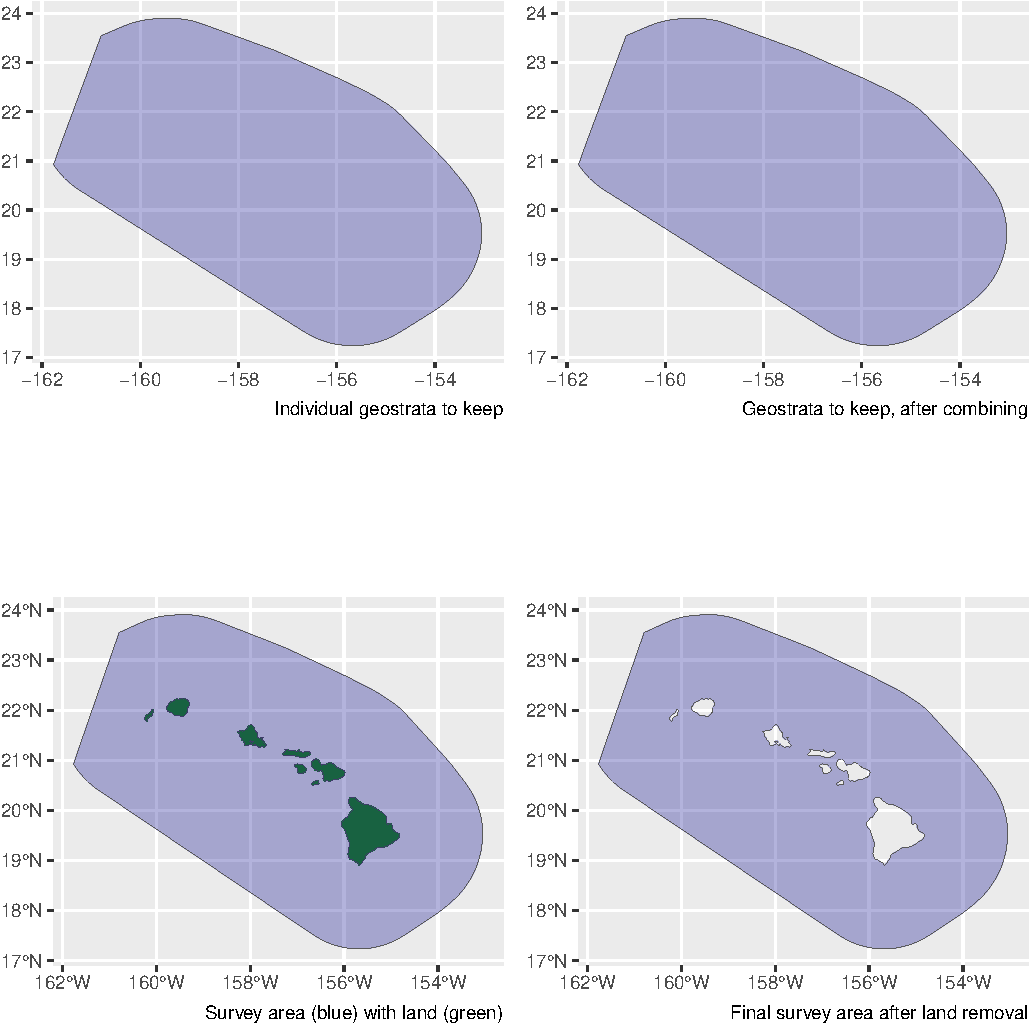
\includegraphics{figures/unnamed-chunk-250-1.pdf}

Say you want to estimate abundance in the pelagic Hawaiian EEZ, ignoring effort and sightings within the Main Hawaiian Islands stratum and accurately removing small islands in northwest Hawaii:

\begin{Shaded}
\begin{Highlighting}[]
\NormalTok{demo }\OtherTok{\textless{}{-}} \FunctionTok{strata\_area}\NormalTok{(}\AttributeTok{strata\_all =}\NormalTok{ cruz}\SpecialCharTok{$}\NormalTok{settings}\SpecialCharTok{$}\NormalTok{strata,}
                    \AttributeTok{strata\_keep =} \FunctionTok{c}\NormalTok{(}\StringTok{\textquotesingle{}HI\_EEZ\textquotesingle{}}\NormalTok{),}
                    \AttributeTok{strata\_remove =} \FunctionTok{c}\NormalTok{(}\StringTok{\textquotesingle{}MHI\textquotesingle{}}\NormalTok{),}
                    \AttributeTok{verbose =} \ConstantTok{FALSE}\NormalTok{)}
\end{Highlighting}
\end{Shaded}

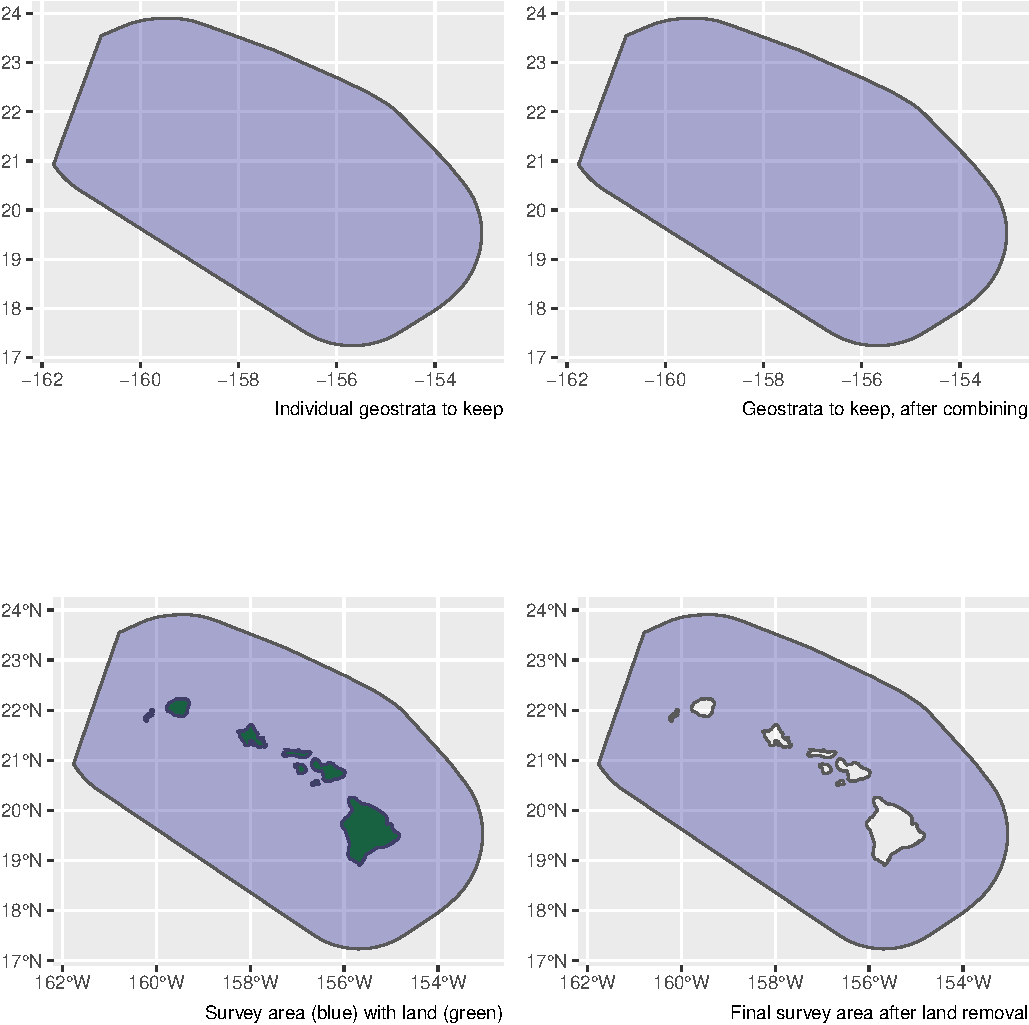
\includegraphics{figures/unnamed-chunk-251-1.pdf}

Say you want to estimate abundance of pelagic bottlenose dolphins within the WHICEAS study area, ignoring the insular stocks:

\begin{Shaded}
\begin{Highlighting}[]
\NormalTok{demo }\OtherTok{\textless{}{-}} \FunctionTok{strata\_area}\NormalTok{(}\AttributeTok{strata\_all =}\NormalTok{ cruz}\SpecialCharTok{$}\NormalTok{settings}\SpecialCharTok{$}\NormalTok{strata,}
                    \AttributeTok{strata\_keep =} \FunctionTok{c}\NormalTok{(}\StringTok{\textquotesingle{}WHICEAS\textquotesingle{}}\NormalTok{),}
                    \AttributeTok{strata\_remove =} \FunctionTok{c}\NormalTok{(}\StringTok{\textquotesingle{}Bottlenose\_KaNi\textquotesingle{}}\NormalTok{,}\StringTok{\textquotesingle{}Bottlenose\_OUFI\textquotesingle{}}\NormalTok{,}\StringTok{\textquotesingle{}Bottlenose\_BI\textquotesingle{}}\NormalTok{),}
                    \AttributeTok{verbose =} \ConstantTok{FALSE}\NormalTok{)}
\end{Highlighting}
\end{Shaded}

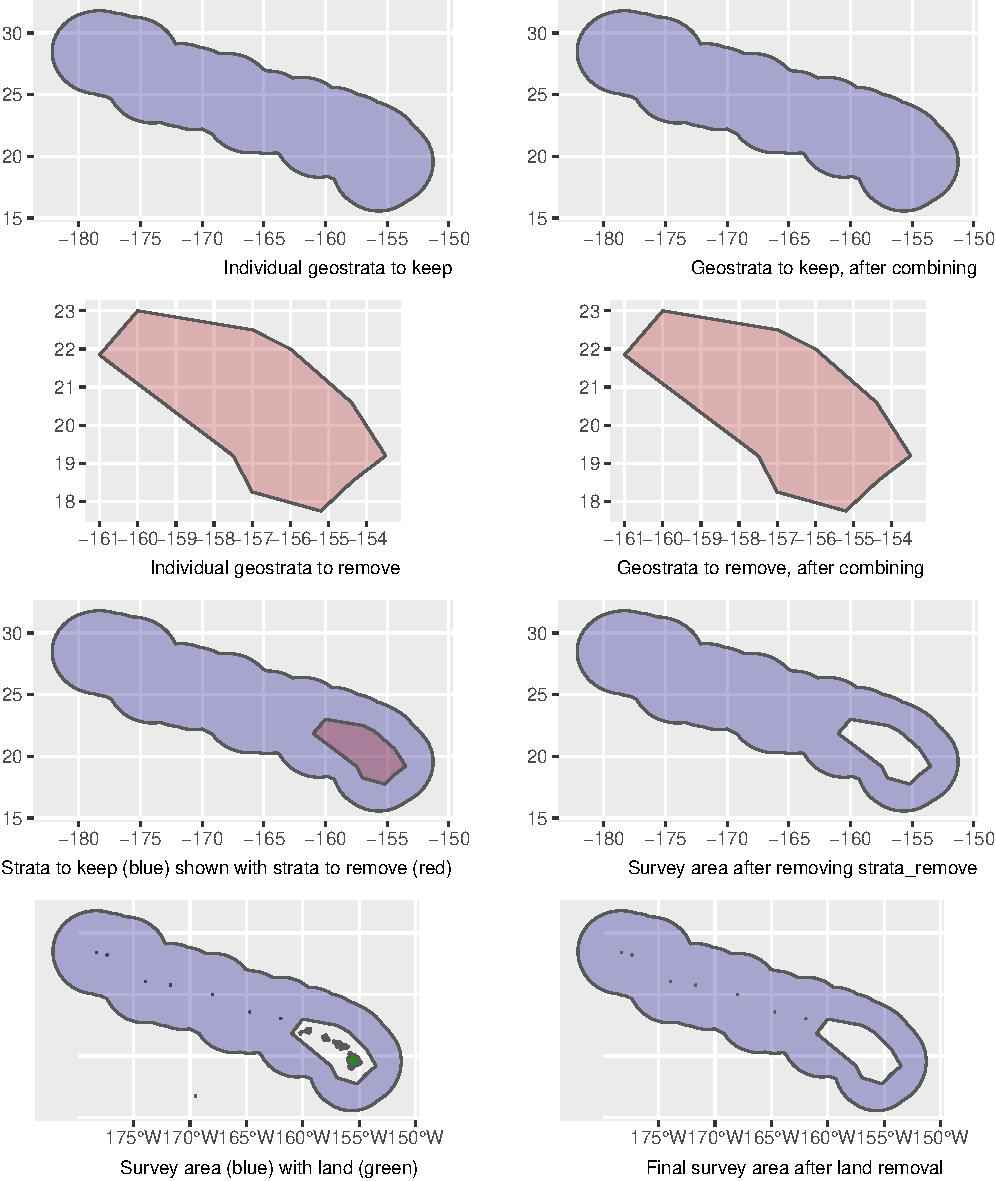
\includegraphics{figures/unnamed-chunk-252-1.pdf}

Say you want to estimate abundance for \emph{only} the insular bottlenose stocks:

\begin{Shaded}
\begin{Highlighting}[]
\NormalTok{demo }\OtherTok{\textless{}{-}} \FunctionTok{strata\_area}\NormalTok{(}\AttributeTok{strata\_all =}\NormalTok{ cruz}\SpecialCharTok{$}\NormalTok{settings}\SpecialCharTok{$}\NormalTok{strata,}
                    \AttributeTok{strata\_keep =} \FunctionTok{c}\NormalTok{(}\StringTok{\textquotesingle{}Bottlenose\_KaNi\textquotesingle{}}\NormalTok{,}\StringTok{\textquotesingle{}Bottlenose\_OUFI\textquotesingle{}}\NormalTok{,}\StringTok{\textquotesingle{}Bottlenose\_BI\textquotesingle{}}\NormalTok{),}
                    \AttributeTok{verbose =} \ConstantTok{FALSE}\NormalTok{)}
\end{Highlighting}
\end{Shaded}

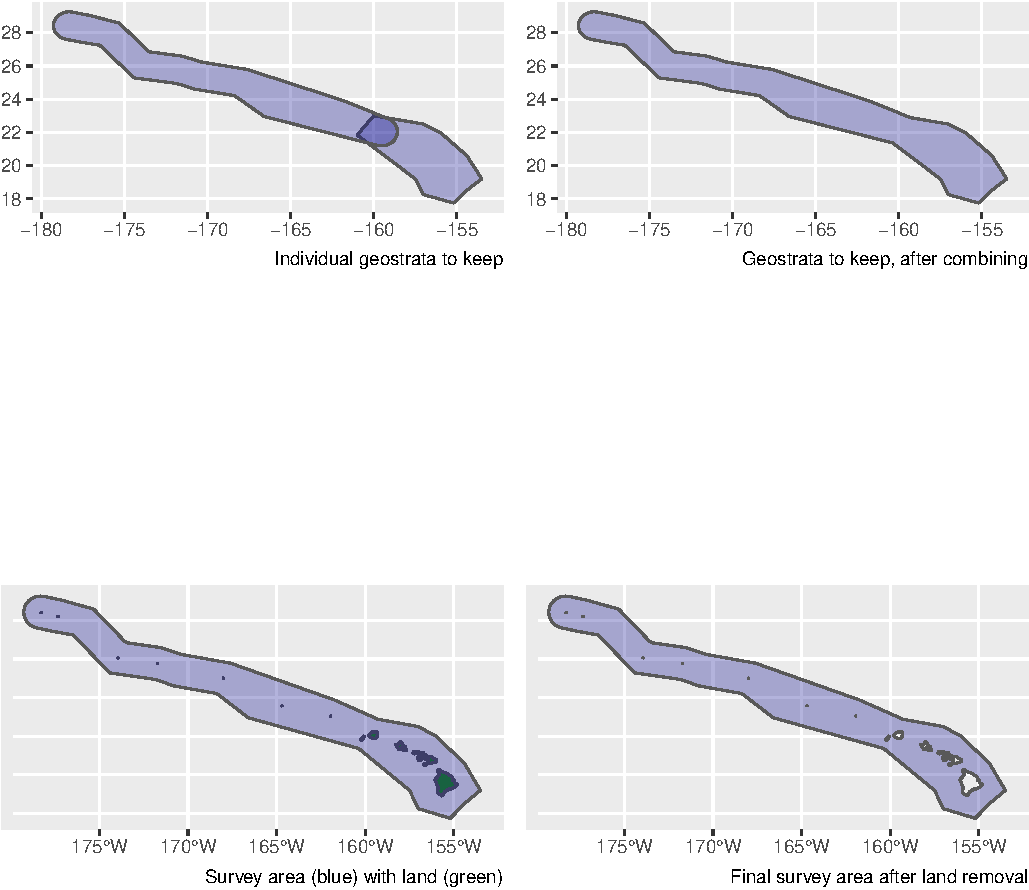
\includegraphics{figures/unnamed-chunk-253-1.pdf}

Say you want to estimate abundance for false killer whales within the Northwest Hawaiian Islands and Main Hawaiian Islands study areas combined, but those geostrata partially overlap:

\begin{Shaded}
\begin{Highlighting}[]
\NormalTok{demo }\OtherTok{\textless{}{-}} \FunctionTok{strata\_area}\NormalTok{(}\AttributeTok{strata\_all =}\NormalTok{ cruz}\SpecialCharTok{$}\NormalTok{settings}\SpecialCharTok{$}\NormalTok{strata,}
                    \AttributeTok{strata\_keep =} \FunctionTok{c}\NormalTok{(}\StringTok{\textquotesingle{}MHI\textquotesingle{}}\NormalTok{,}\StringTok{\textquotesingle{}NWHI\textquotesingle{}}\NormalTok{),}
                    \AttributeTok{verbose =} \ConstantTok{FALSE}\NormalTok{)}
\end{Highlighting}
\end{Shaded}

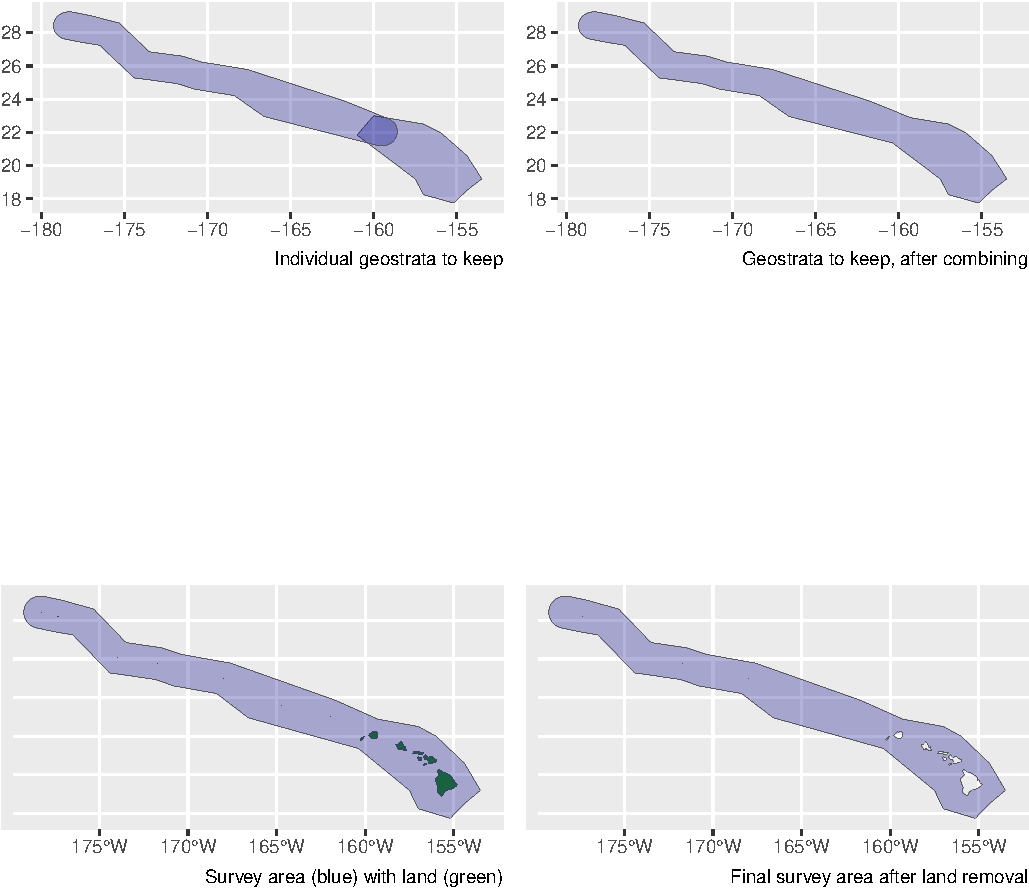
\includegraphics{figures/unnamed-chunk-254-1.pdf}

Say you want to estimate abundance for the Hawaiian EEZ \emph{outside} of those partially overlapping geostrata:

\begin{Shaded}
\begin{Highlighting}[]
\NormalTok{demo }\OtherTok{\textless{}{-}} \FunctionTok{strata\_area}\NormalTok{(}\AttributeTok{strata\_all =}\NormalTok{ cruz}\SpecialCharTok{$}\NormalTok{settings}\SpecialCharTok{$}\NormalTok{strata,}
                    \AttributeTok{strata\_keep =} \StringTok{\textquotesingle{}HI\_EEZ\textquotesingle{}}\NormalTok{,}
                    \AttributeTok{strata\_remove =} \FunctionTok{c}\NormalTok{(}\StringTok{\textquotesingle{}MHI\textquotesingle{}}\NormalTok{,}\StringTok{\textquotesingle{}NWHI\textquotesingle{}}\NormalTok{),}
                    \AttributeTok{verbose =} \ConstantTok{FALSE}\NormalTok{)}
\end{Highlighting}
\end{Shaded}

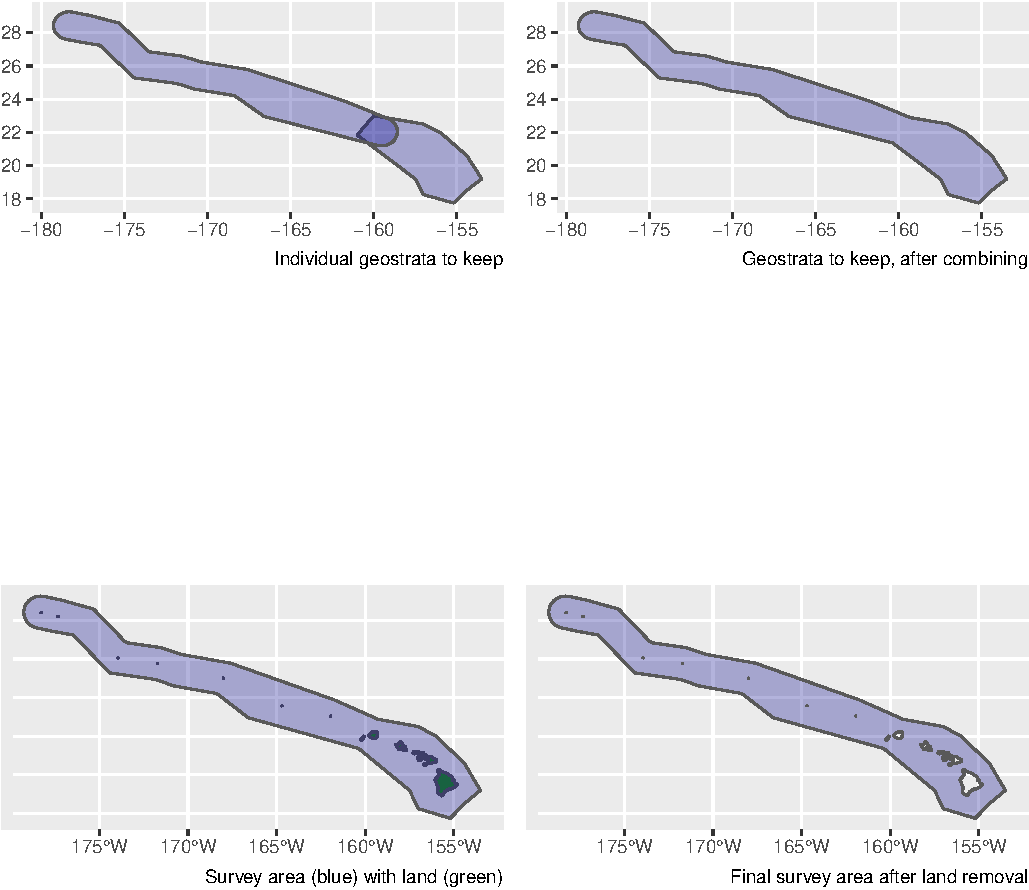
\includegraphics{figures/unnamed-chunk-255-1.pdf}

\hypertarget{g0-estimation}{%
\subsection*{\texorpdfstring{\emph{g(0)} estimation}{g(0) estimation}}\label{g0-estimation}}
\addcontentsline{toc}{subsection}{\emph{g(0)} estimation}

If you want \texttt{lta()} to calculate a weighted \emph{g(0)} estimate (and associated CV) that is specific to the conditions associated with your \texttt{estimates} sub-list parameters, all you need to do is provide the \texttt{Rg0} input. When you do this, the \texttt{lta()} function will find the \texttt{Rg0} values associated with the species code(s) in your \texttt{estimates} sub-list, then calculate weighted \emph{g(0)} and its CV using the \texttt{LTabundR} function, \texttt{g0\_weighted()}, which we discussed and demonstrated on the previous page.

If \texttt{lta()} can't find your species code in the \texttt{Rg0} table you provide, it will give up and assume that \texttt{g(0)} is 1.0 and that \texttt{g0\_cv} is 0.0.

If your \texttt{estimates} sub-list has a \texttt{alt\_g0\_spp} slot, \texttt{lta()} will use that species code instead to filter the \texttt{Rg0} table.

If your \texttt{estimates} sub-list has a \texttt{combine\_g0} slot that is \texttt{TRUE}, \texttt{lta()} will filter the \texttt{Rg0} table using all species codes you provide. If that filtration results in multiple \texttt{Rg0} species being found, weighted \emph{g(0)} will be calculated for each of those species separately, then those \emph{g(0)} estimates will be combined using a geometric mean (using the \texttt{LTabundR} function \texttt{g0\_combine()}). If \texttt{combine\_g0} is \texttt{FALSE}, only the first species code provided in your \texttt{estimates} sub-list will be used to filter \texttt{Rg0}.

If you want to supply a weighted \emph{g(0)} estimate and its CV yourself, you can add the \texttt{g0} and \texttt{g0\_cv} slots to your \texttt{estlimates} sublist, as explained above.

If you want to coerce \emph{g(0)} to be assumed to be 1.0 (with CV = 0.0), you can either (1) \emph{not} supply the \texttt{Rg0} input, or (2) manually specify the \texttt{g0} and \texttt{g0\_cv} slots in your \texttt{estimates} sub-list accordingly.

\hypertarget{covariates-in-detection-function-estimation}{%
\subsection*{Covariates in detection function estimation}\label{covariates-in-detection-function-estimation}}
\addcontentsline{toc}{subsection}{Covariates in detection function estimation}

Before detection functions are modelled, any covariates supplied by the user and specified as a factor are first tested for eligibility. Only factors with at least two levels (or whatever you specified with \texttt{df\_settings\$covariates\_levels}) and 10 observations in each level (or whatever you specified with \texttt{df\_settings\$covariates\_n\_per\_level}) are eligible for inclusion.

\hypertarget{fitting-a-detection-function}{%
\subsection*{Fitting a detection function}\label{fitting-a-detection-function}}
\addcontentsline{toc}{subsection}{Fitting a detection function}

The detection function is estimated using functions in the package \texttt{mrds}, primarily the main function \texttt{mrds::ddf()}, which uses a Horvitz-Thompson-like estimator to predict the probability of detection for each sighting. If multiple base key functions (e.g., half-normal or hazard-rate) are provided, and/or if covariates are specified, model fitting is done in a forward stepwise procedure:

\begin{itemize}
\tightlist
\item
  In the first round, the base model (no covariates, i.e., \texttt{"\textasciitilde{}1"}) is fit first.\\
\item
  In the second round, each covariate is added one at a time; at the end of the round, the covariate, if any, that produces the lowest AIC below the AIC from the previous round is added to the formula.\\
\item
  This process is repeated in subsequent rounds, adding a new covariate term in each round, until the AIC no longer improves.
\item
  If a second base key is provided, the process is repeated for that second key.
\end{itemize}

All models within \texttt{delta\_aic} of the model with the lowest AIC qualify as best-fitting models. The best-fitting model(s) is(are) then used to estimate the Effective Strip half-Width (ESW) based on the covariates associated with each sighting.

If multiple best-fitting models occur, we will find the average ESW for each sighting across all models, using a weighted mean approach in which we weight according to model AIC. To turn off this model averaging step, set \texttt{delta\_aic} to \texttt{0} to avoid passing multiple models to the abundance estimation stage.

Note that if \texttt{LnSsTot} is included as a covariate, the function will (1) check to see if the \texttt{sightings} dataframe has a column named \texttt{ss\_valid} (all \texttt{cruz} objects do), then, if so, (2) filter \texttt{sightings} only to rows where \texttt{ss\_valid} is \texttt{TRUE}, meaning the school size estimate for that sighting is a valid estimate.

This stage of the \texttt{lta()} command is executed within a backend function, \texttt{LTabundR::fit\_df()}, which has its own documentation for your reference.

\hypertarget{estimating-density-abundance}{%
\subsection*{Estimating density \& abundance}\label{estimating-density-abundance}}
\addcontentsline{toc}{subsection}{Estimating density \& abundance}

Estimates are produced for various combinations of species, regions, and years, according to the arguments specified in your \texttt{estimates} list(s). Before these estimates are produced, we filter the data used to fit the detection function to strictly systematic (design-based) effort (i.e., \texttt{EffType\ =\ "S"}), in which standard protocols are in use (i.e., \texttt{OnEffort\ =\ TRUE}) and the Beaufort sea state is less than 7 (though these controls can be modified using the \texttt{lta()} inputs \texttt{abund\_eff\_types} and \texttt{abund\_bft\_range} (see above).

Note that if \texttt{sightings} has a column named \texttt{ss\_valid} (all standard \texttt{cruz} objects do) and any of the rows in that column are \texttt{FALSE}, those rows will have their \texttt{best} school size estimate (which will be \texttt{NA} or \texttt{1}, since they are invalid) replaced by the mean best estimate for their respective species.

This stage of the \texttt{lta()} command is executed within a back-end function, \texttt{LTabundR::abundance()}, which has its own documentation for your reference.

\hypertarget{bootstrap-variance-estimation}{%
\subsection*{Bootstrap variance estimation}\label{bootstrap-variance-estimation}}
\addcontentsline{toc}{subsection}{Bootstrap variance estimation}

If the \texttt{bootstraps} input value is greater than 1, bootstrap variance estimation will be attempted. In each bootstrap iteration, survey segments are re-sampled with replacement before fitting the detection function and estimating density/abundance. Re-sampling is done in a routine that preserves the proportion of segments from each geostratum.

Note that the entire process is repeated in each bootstrap: step-wise fitting of the detection function, averaging of the best-fitting models, and density/abundance estimation for all species/region/year combinations specified in your \texttt{estimates} input. At the end of the bootstrap process, results are summarized for each species/region/year combination. 95\% confidence intervals are calculated using the BCA method (package \texttt{coxed}, function \texttt{bca()}).

\hypertarget{g0-values-during-bootstrapping}{%
\subsection*{\texorpdfstring{\texttt{g(0)} values during bootstrapping}{g(0) values during bootstrapping}}\label{g0-values-during-bootstrapping}}
\addcontentsline{toc}{subsection}{\texttt{g(0)} values during bootstrapping}

When conducting the non-parametric bootstrap routine to estimate the CV of density and abundance, uncertainty is incorporated into the g(0) value in each iteration using a parametric bootstrapping subroutine: First, a logit-transformed distribution is modeled based upon the mean and CV of g(0) provided by the user in the \texttt{estimates} input (see documentation for \texttt{LTabundR::g0\_optimize()} for details on this step). This modeled distribution is used to randomly draw a g(0) value for each iteration of the density/abundance bootstrap routine. In this way, the uncertainty in g(0) is propagated into uncertainty in density/abundance.

\hypertarget{destratify}{%
\chapter{Stratified analysis}\label{destratify}}

Field surveys are sometimes stratified such that trackline design and/or density can differ substantially across regions. Also, analysts may sometimes wish to estimate density/abundance for individual regions separately, regardless of design stratification.

On the previous page, we demonstrated how to accommodate a stratified analysis by providing an \texttt{estimates} sub-list for each geostratum.

For example, in 2002 the Hawaiian EEZ was surveyed with different effort intensity in the Main Hawaiian Islands region compared to pelagic waters.

Here is the code that generates density/abundance estimates of striped dolphins in 2002 (stratified) and 2010 (unstratified), with only 10 bootstrap iterations:

\begin{Shaded}
\begin{Highlighting}[]
\CommentTok{\# Survey data}
\FunctionTok{data}\NormalTok{(}\StringTok{"cnp\_150km\_1986\_2020"}\NormalTok{)}
\NormalTok{cruz }\OtherTok{\textless{}{-}}\NormalTok{ cnp\_150km\_1986\_2020}

\CommentTok{\# Rg0 table}
\FunctionTok{data}\NormalTok{(}\StringTok{"g0\_results"}\NormalTok{)}
\NormalTok{Rg0 }\OtherTok{\textless{}{-}}\NormalTok{ g0\_results}

\CommentTok{\# Detection function filters}
\NormalTok{fit\_filters }\OtherTok{\textless{}{-}} \FunctionTok{list}\NormalTok{(}\AttributeTok{spp =} \FunctionTok{c}\NormalTok{(}\StringTok{\textquotesingle{}013\textquotesingle{}}\NormalTok{, }\StringTok{\textquotesingle{}026\textquotesingle{}}\NormalTok{, }\StringTok{\textquotesingle{}031\textquotesingle{}}\NormalTok{), }
                   \AttributeTok{pool =} \StringTok{\textquotesingle{}Multi{-}species pool 1\textquotesingle{}}\NormalTok{,}
                   \AttributeTok{cohort =} \StringTok{\textquotesingle{}all\textquotesingle{}}\NormalTok{,}
                   \AttributeTok{truncation\_distance =} \DecValTok{5}\NormalTok{,}
                   \AttributeTok{other\_species =} \StringTok{\textquotesingle{}remove\textquotesingle{}}\NormalTok{)}

\CommentTok{\# Detection function settings}
\NormalTok{df\_settings }\OtherTok{\textless{}{-}} \FunctionTok{list}\NormalTok{(}\AttributeTok{covariates =} \FunctionTok{c}\NormalTok{(}\StringTok{\textquotesingle{}bft\textquotesingle{}}\NormalTok{,}\StringTok{\textquotesingle{}lnsstot\textquotesingle{}}\NormalTok{,}\StringTok{\textquotesingle{}cruise\textquotesingle{}}\NormalTok{,}\StringTok{\textquotesingle{}year\textquotesingle{}}\NormalTok{,}\StringTok{\textquotesingle{}ship\textquotesingle{}}\NormalTok{,}\StringTok{\textquotesingle{}species\textquotesingle{}}\NormalTok{),}
                   \AttributeTok{covariates\_factor =} \FunctionTok{c}\NormalTok{(}\ConstantTok{FALSE}\NormalTok{, }\ConstantTok{FALSE}\NormalTok{, }\ConstantTok{TRUE}\NormalTok{, }\ConstantTok{TRUE}\NormalTok{, }\ConstantTok{TRUE}\NormalTok{, }\ConstantTok{TRUE}\NormalTok{),}
                   \AttributeTok{covariates\_levels =} \DecValTok{2}\NormalTok{,}
                   \AttributeTok{covariates\_n\_per\_level =} \DecValTok{10}\NormalTok{,}
                   \AttributeTok{detection\_function\_base =} \StringTok{\textquotesingle{}hn\textquotesingle{}}\NormalTok{,}
                   \AttributeTok{base\_model =} \StringTok{\textquotesingle{}\textasciitilde{}1\textquotesingle{}}\NormalTok{,}
                   \AttributeTok{delta\_aic =} \DecValTok{2}\NormalTok{)}

\CommentTok{\# Estimates}
\NormalTok{estimates }\OtherTok{\textless{}{-}} \FunctionTok{list}\NormalTok{(}
    \FunctionTok{list}\NormalTok{(}\AttributeTok{spp =} \StringTok{\textquotesingle{}013\textquotesingle{}}\NormalTok{,}
         \AttributeTok{title =} \StringTok{\textquotesingle{}Striped dolphin\textquotesingle{}}\NormalTok{,}
         \AttributeTok{years =} \DecValTok{2002}\NormalTok{,}
         \AttributeTok{regions =} \StringTok{\textquotesingle{}MHI\textquotesingle{}}\NormalTok{),}
    \FunctionTok{list}\NormalTok{(}\AttributeTok{spp =} \StringTok{\textquotesingle{}013\textquotesingle{}}\NormalTok{,}
         \AttributeTok{title =} \StringTok{\textquotesingle{}Striped dolphin\textquotesingle{}}\NormalTok{,}
         \AttributeTok{years =} \DecValTok{2002}\NormalTok{,}
         \AttributeTok{regions =} \StringTok{\textquotesingle{}HI\_EEZ\textquotesingle{}}\NormalTok{,}
         \AttributeTok{regions\_remove =} \StringTok{\textquotesingle{}MHI\textquotesingle{}}\NormalTok{),}
    \FunctionTok{list}\NormalTok{(}\AttributeTok{spp =} \StringTok{\textquotesingle{}013\textquotesingle{}}\NormalTok{,}
         \AttributeTok{title =} \StringTok{\textquotesingle{}Striped dolphin\textquotesingle{}}\NormalTok{,}
         \AttributeTok{years =} \DecValTok{2010}\NormalTok{,}
         \AttributeTok{regions =} \StringTok{\textquotesingle{}HI\_EEZ\textquotesingle{}}\NormalTok{))}

\CommentTok{\# Run it}
\NormalTok{results }\OtherTok{\textless{}{-}} \FunctionTok{lta}\NormalTok{(cruz, Rg0, }
\NormalTok{               fit\_filters, df\_settings, estimates, }
               \AttributeTok{bootstraps =} \DecValTok{10}\NormalTok{)}

\CommentTok{\# Save it locally}
\FunctionTok{saveRDS}\NormalTok{(results, }\AttributeTok{file=}\StringTok{\textquotesingle{}lta/multispecies\_pool\_1.RData\textquotesingle{}}\NormalTok{)}
\end{Highlighting}
\end{Shaded}

Let's read these results back in using the \texttt{LTabundR} function \texttt{lta\_enlist()}, which stores LTA results in a flexible list structure.

\begin{Shaded}
\begin{Highlighting}[]
\NormalTok{ltas }\OtherTok{\textless{}{-}} \FunctionTok{lta\_enlist}\NormalTok{(}\StringTok{\textquotesingle{}lta/\textquotesingle{}}\NormalTok{)}
\end{Highlighting}
\end{Shaded}

As these results stand, 2002 estimates are stratified into 2 separate regions:

\begin{Shaded}
\begin{Highlighting}[]
\NormalTok{(ltas }\SpecialCharTok{\%\textgreater{}\%} \FunctionTok{lta\_report}\NormalTok{(}\AttributeTok{verbose =} \ConstantTok{FALSE}\NormalTok{))}\SpecialCharTok{$}\NormalTok{table4}
                         \DecValTok{2002}\NormalTok{ (HI\_EEZ) }\SpecialCharTok{{-}}\NormalTok{ (MHI)                       }\DecValTok{2002}
\DecValTok{1}\NormalTok{ Species or category Density        Abundance   CV        }\DecValTok{95}\NormalTok{\% CI Density}
\DecValTok{2}\NormalTok{     Striped dolphin    }\FloatTok{9.22}           \DecValTok{20}\NormalTok{,}\DecValTok{855} \FloatTok{0.26} \DecValTok{21}\NormalTok{,}\DecValTok{638{-}44}\NormalTok{,}\DecValTok{648}    \FloatTok{8.44}
\NormalTok{      (MHI)                 }\DecValTok{2010}\NormalTok{  (HI\_EEZ)                   }
\DecValTok{1}\NormalTok{ Abundance   CV  }\DecValTok{95}\SpecialCharTok{\% CI Density Abundance   CV        95\%}\NormalTok{ CI}
\DecValTok{2}     \DecValTok{1}\NormalTok{,}\DecValTok{790} \FloatTok{0.81} \DecValTok{0{-}3}\NormalTok{,}\DecValTok{854}   \FloatTok{14.36}    \DecValTok{35}\NormalTok{,}\DecValTok{527} \FloatTok{0.27} \DecValTok{35}\NormalTok{,}\DecValTok{038{-}77}\NormalTok{,}\DecValTok{911}
\end{Highlighting}
\end{Shaded}

Now let's process these LTA results through an \texttt{LTabundR} function, \texttt{lta\_destratify()}, which will combine the separate regional estimates from 2002 into a single estimate for the year.

\begin{Shaded}
\begin{Highlighting}[]
\NormalTok{ltas\_2a }\OtherTok{\textless{}{-}}
  \FunctionTok{lta\_destratify}\NormalTok{(ltas,}
               \AttributeTok{years =} \DecValTok{2002}\NormalTok{,}
               \AttributeTok{combine\_method =} \StringTok{\textquotesingle{}arithmetic\textquotesingle{}}\NormalTok{,}
               \AttributeTok{new\_region =} \StringTok{\textquotesingle{}(HI\_EEZ)\textquotesingle{}}\NormalTok{)}
\end{Highlighting}
\end{Shaded}

The \texttt{new\_region} argument specifies how to refer to the combined region. In this case we want the 2002 study area to be named the same as the unstratified 2010 study area, hence \texttt{"(HI\_EEZ)"}. The \texttt{combine\_method} argument is explained below.

Now let's re-check the summary table:

\begin{Shaded}
\begin{Highlighting}[]
\NormalTok{(ltas\_2a }\SpecialCharTok{\%\textgreater{}\%} \FunctionTok{lta\_report}\NormalTok{(}\AttributeTok{verbose=}\ConstantTok{FALSE}\NormalTok{))}\SpecialCharTok{$}\NormalTok{table4}
                         \DecValTok{2002}\NormalTok{  (HI\_EEZ)                      }\DecValTok{2010}\NormalTok{  (HI\_EEZ)}
\DecValTok{1}\NormalTok{ Species or category Density Abundance   CV       }\DecValTok{95}\NormalTok{\% CI Density Abundance}
\DecValTok{2}\NormalTok{     Striped dolphin    }\FloatTok{9.15}    \DecValTok{22}\NormalTok{,}\DecValTok{646} \FloatTok{0.74} \DecValTok{6}\NormalTok{,}\DecValTok{176{-}83}\NormalTok{,}\DecValTok{039}   \FloatTok{14.36}    \DecValTok{35}\NormalTok{,}\DecValTok{527}
                    
\DecValTok{1}\NormalTok{   CV        }\DecValTok{95}\NormalTok{\% CI}
\DecValTok{2} \FloatTok{0.27} \DecValTok{35}\NormalTok{,}\DecValTok{038{-}77}\NormalTok{,}\DecValTok{911}
\end{Highlighting}
\end{Shaded}

There is now only one set of columns for 2002, and the values therein are combinations of the stratified regions.

The ``de-stratification'' routine within \texttt{lta\_destratify()} sums abundance estimates across regions to get combined abundance. To estimate density in the combined regions, the function uses weighted averaging in which the area of a geostratum serves as its weight. To estimate CV and confidence interval of the combined result, the function uses one of two \texttt{combine\_methods} (this is an argument in the function). The default method is \texttt{"arithmetic"}, which uses classic formulae to estimate the combined variance and the corresponding confidence interval. This is done in a way that allows multiple geostrata to be combined, not just two.

The second option, \texttt{"bootstrap"}, uses an iterative method that draws bootstrap samples, with replacement, from the bootstrap estimate of density within each stratified region.

\begin{Shaded}
\begin{Highlighting}[]
\NormalTok{ltas\_2b }\OtherTok{\textless{}{-}}
  \FunctionTok{lta\_destratify}\NormalTok{(ltas,}
               \AttributeTok{years =} \DecValTok{2002}\NormalTok{,}
               \AttributeTok{combine\_method =} \StringTok{\textquotesingle{}bootstrap\textquotesingle{}}\NormalTok{,}
               \AttributeTok{new\_region =} \StringTok{\textquotesingle{}(HI\_EEZ)\textquotesingle{}}\NormalTok{)}
\end{Highlighting}
\end{Shaded}

\begin{Shaded}
\begin{Highlighting}[]
\NormalTok{(ltas\_2b }\SpecialCharTok{\%\textgreater{}\%} \FunctionTok{lta\_report}\NormalTok{(}\AttributeTok{verbose=}\ConstantTok{FALSE}\NormalTok{))}\SpecialCharTok{$}\NormalTok{table4}
                         \DecValTok{2002}\NormalTok{  (HI\_EEZ)                       }\DecValTok{2010}\NormalTok{  (HI\_EEZ)}
\DecValTok{1}\NormalTok{ Species or category Density Abundance   CV        }\DecValTok{95}\NormalTok{\% CI Density Abundance}
\DecValTok{2}\NormalTok{     Striped dolphin    }\FloatTok{9.15}    \DecValTok{22}\NormalTok{,}\DecValTok{646} \FloatTok{0.23} \DecValTok{22}\NormalTok{,}\DecValTok{484{-}48}\NormalTok{,}\DecValTok{617}   \FloatTok{14.36}    \DecValTok{35}\NormalTok{,}\DecValTok{527}
                    
\DecValTok{1}\NormalTok{   CV        }\DecValTok{95}\NormalTok{\% CI}
\DecValTok{2} \FloatTok{0.27} \DecValTok{35}\NormalTok{,}\DecValTok{038{-}77}\NormalTok{,}\DecValTok{911}
\end{Highlighting}
\end{Shaded}

Note that use of \texttt{lta\_destratify()} only makes sense if the stratified regions have zero overlap.

\hypertarget{trend-analysis}{%
\chapter{Trend analysis}\label{trend-analysis}}

When a species' density appears to change dramatically from one survey year to the next, it could be due to several factors: the species' abundance may have changed; its range may have shifted; or the timing of its migratory movements may have shifted. This apparent change could also be due solely to random chance: you can sample the exact same population in two different surveys, and you are liable to produce different abundance estimates due simply to random variation in how often you encounter your target species. In other words, \emph{random variation in the encounter rate} may lead you to estimate a change in abundance, when in fact there is no change.

For this reason, whenever you suspect that abundance has changed between years -- i.e., whenever the confidence intervals for two years do not overlap -- it is good practice to carry out follow-up tests. One such test was developed in (\href{https://www.fisheries.noaa.gov/inport/item/59592}{Bradford et al.~2020} and Bradford et al.~(2021). That test has been provided in \texttt{LTabundR} with the function \texttt{er\_simulator()}, which refers to a simulation-based test of random variation in the \textbf{e}ncounter \textbf{r}ate (ER).

This function uses randomization simulations to test for the probability that year-to-year changes observed in a species' encounter rate are due to random sampling variation (and not actual change in the encounter rate). More specifcially, this function uses bootstrap sampling of survey segments to see if random variation in sampling could possibly produce an apparent but immaterial change in encounter rate across years.

You will find full analytical details in the Appendix to Bradford et al.~(2020) for analytical details, but briefly: in each bootstrap iteration, survey segments are resampled in a way that preserves the proportion of effort occurring within each geostratum in the data. The resampled data are used to calculate the overall ER across all survey years, since the null hypothesis is that the ER does not change across years. This overall ER is used to predict the number of sightings in each year, based on the distance covered by the resampled segments in each year. This process is repeated (typically hundreds to thousands of times) to produce a distribution of predicted sighting counts in each year. This distribution reflects the range of ERs that could be possible due simply to random variation and \emph{not} to underlying changes in abundance. These distributions are compared to the actual number of sightings observed in their respective year. The fraction of simulated sightings counts that are more extreme than the observed count reflects the probability that the observed count is due to random sample variation alone.

For example, Bradford et al.~(2021) found non-overlapping confidence intervals in their estimates of Bryde's whale abundance in 2002, 2010, and 2017. To test for the significance of these trends, they carried out the ``ER simulator'' routine described above. In \texttt{LTabundR}, we would carry out the same analysis as follows:

Take your processed data:

\begin{Shaded}
\begin{Highlighting}[]
\FunctionTok{data}\NormalTok{(cnp\_150km\_1986\_2020)}
\NormalTok{cruz }\OtherTok{\textless{}{-}}\NormalTok{ cnp\_150km\_1986\_2020}
\end{Highlighting}
\end{Shaded}

Filter it to systematic effort in the years of interest:

\begin{Shaded}
\begin{Highlighting}[]
\NormalTok{cruzi }\OtherTok{\textless{}{-}} 
  \FunctionTok{filter\_cruz}\NormalTok{(cruz,}
              \AttributeTok{analysis\_only =} \ConstantTok{TRUE}\NormalTok{,}
              \AttributeTok{years =} \FunctionTok{c}\NormalTok{(}\DecValTok{2002}\NormalTok{, }\DecValTok{2010}\NormalTok{, }\DecValTok{2017}\NormalTok{),}
              \AttributeTok{regions =} \StringTok{\textquotesingle{}HI\_EEZ\textquotesingle{}}\NormalTok{,}
              \AttributeTok{eff\_types =} \StringTok{\textquotesingle{}S\textquotesingle{}}\NormalTok{,}
              \AttributeTok{bft\_range =} \DecValTok{0}\SpecialCharTok{:}\DecValTok{6}\NormalTok{)}
\end{Highlighting}
\end{Shaded}

Conduct the ER simulation, passing the species code for the Bryde's whale (\texttt{"072"}). For the purposes of this example, we will only use 100 iterations.

\begin{Shaded}
\begin{Highlighting}[]
\NormalTok{er\_results }\OtherTok{\textless{}{-}} 
  \FunctionTok{er\_simulator}\NormalTok{(}\AttributeTok{spp =} \StringTok{\textquotesingle{}072\textquotesingle{}}\NormalTok{, }\AttributeTok{cruz =}\NormalTok{ cruzi, }\AttributeTok{iterations =} \DecValTok{100}\NormalTok{)}
\end{Highlighting}
\end{Shaded}

This routine provides a list with two slots:

\begin{Shaded}
\begin{Highlighting}[]
\NormalTok{er\_results }\SpecialCharTok{\%\textgreater{}\%}\NormalTok{ names}
\NormalTok{[}\DecValTok{1}\NormalTok{] }\StringTok{"summary"} \StringTok{"details"}
\end{Highlighting}
\end{Shaded}

The \texttt{summary} slot returns the p-value for each year, i.e., the chances that the observed number of sightings was due purely to random variation in the encounter rate.

\begin{Shaded}
\begin{Highlighting}[]
\NormalTok{er\_results}\SpecialCharTok{$}\NormalTok{summary}
\NormalTok{  years observed    p}
\DecValTok{1}  \DecValTok{2002}      \DecValTok{158} \FloatTok{0.96}
\DecValTok{2}  \DecValTok{2010}      \DecValTok{210} \FloatTok{0.00}
\DecValTok{3}  \DecValTok{2017}      \DecValTok{146} \FloatTok{0.97}
\end{Highlighting}
\end{Shaded}

In this example, the encounter rates observed in 2002 and 2010 are very likely due to some process \emph{other} than random variation in the encounter rate, such as range shifts, seasonal movement timing shifts, and/or changes in abundance. However, the observed encounter rate in 2017 could easily be explained by random variation in the ER.

The \texttt{details} slot returns the simulation predictions for each year, which can be used to replicate the histograms that are printed when the function is run.

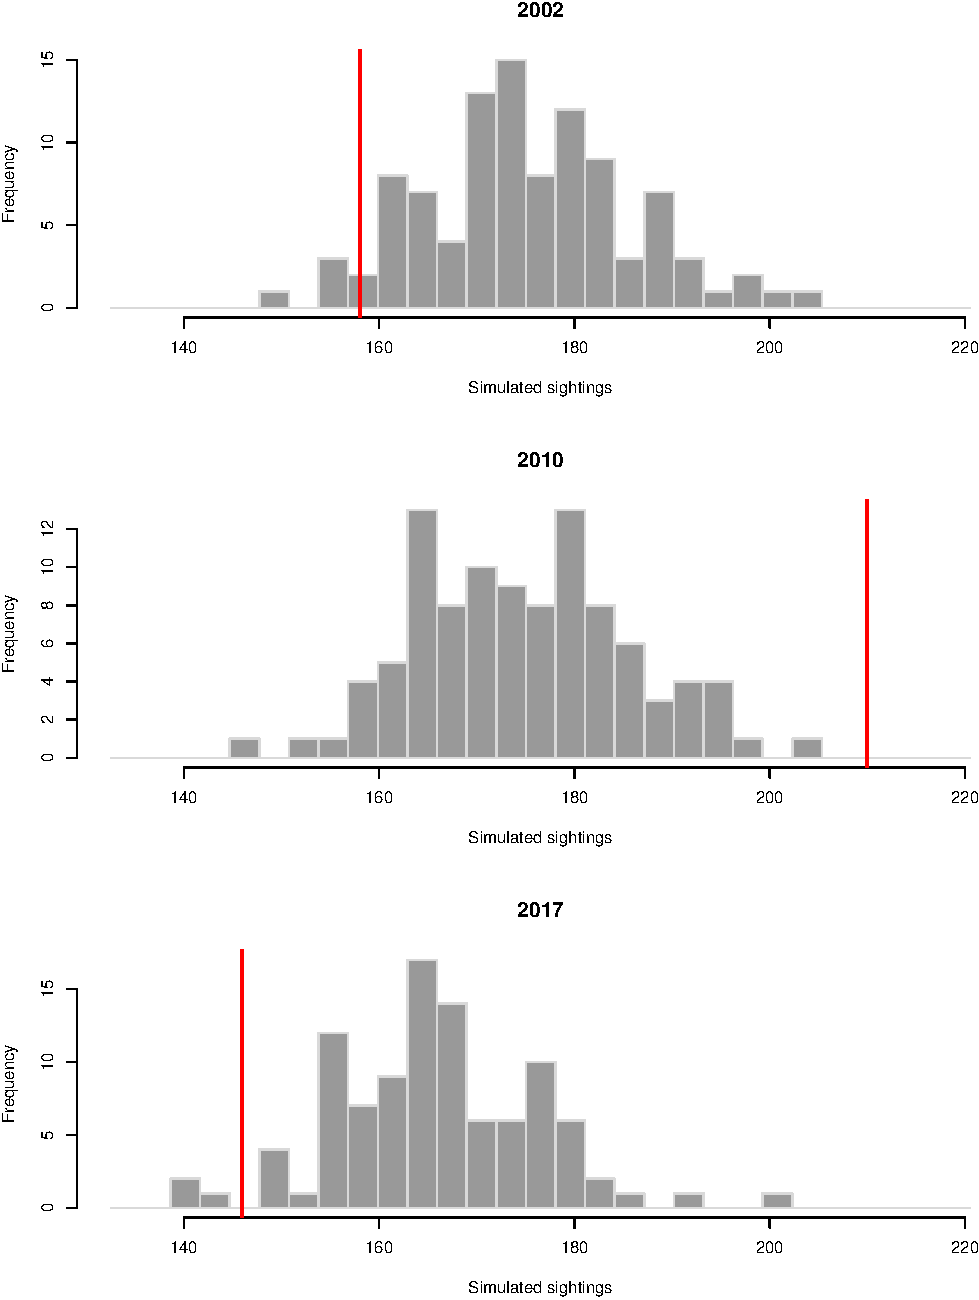
\includegraphics{figures/unnamed-chunk-272-1.pdf}

A dataframe with a row for each year. Columns provide the number of observations of the species of interest during systematic effort, and the p-value of the test. The p-value represents the fraction of simulated encounter rates that exceed the observed encounter rate.

\hypertarget{subgroups}{%
\chapter{Subgroup-based analysis}\label{subgroups}}

False killer whales (\emph{Pseudorca crassidens}) are rare and occur in dispersed subgroups, which complicates conventional distance sampling approaches to line-transect analysis. To better estimate their abundance, in 2010 the Pacific Islands Fisheries Science Center (PIFSC) initiated a sub-group protocol referred to as the ``PC Protocol'', a reference to the species' scientific name.

To conduct line-transect analysis with this sub-group-based protocol, a method was developed in 2014 - 2017
To handle this, a separate, \emph{subgroup-based} analytical approach was developed in 2014 - 2017, then updated in 2020 (\href{https://www.fisheries.noaa.gov/inport/item/59592}{Bradford et al.~2020}).

An additional complication is that false killer whales in Hawaiian waters belong to two discrete populations -- the Northwest Hawaiian Islands (NWHI) population and a pelagic population -- whose ranges partially overlap, which means that population assignment cannot always be based simply on the geographic location of sightings. When geographic inference of population is not possible, biopsy-sampled genetics, photo-identification, and acoustics are used to assign each sighting to a population \emph{post-hoc}.

To accommodate these special circumstances with an appropriate balance of flexibility and efficiency, \texttt{LTabundR} includes a function named \texttt{lta\_subgroup()}, whose use will look something like this:

\begin{Shaded}
\begin{Highlighting}[]
\FunctionTok{lta\_subgroup}\NormalTok{(df\_sits,}
\NormalTok{             truncation\_distance,}
\NormalTok{             ss,}
\NormalTok{             cruz10,}
\NormalTok{             g0\_spp,}
\NormalTok{             g0\_truncation,}
\NormalTok{             g0\_pool\_bft,}
             \AttributeTok{g0\_jackknife\_fraction =} \FloatTok{0.1}\NormalTok{,}
\NormalTok{             density\_segments,}
\NormalTok{             density\_das,}
\NormalTok{             density\_sightings,}
\NormalTok{             abundance\_area,}
             \AttributeTok{iterations =} \DecValTok{1000}\NormalTok{,}
             \AttributeTok{output\_dir =} \StringTok{\textquotesingle{}../test\_code/subgroup/\textquotesingle{}}\NormalTok{,}
             \AttributeTok{toplot =} \ConstantTok{TRUE}\NormalTok{,}
             \AttributeTok{verbose =} \ConstantTok{TRUE}\NormalTok{,}
             \AttributeTok{density\_bootstraps =} \DecValTok{10000}\NormalTok{)}
\end{Highlighting}
\end{Shaded}

We will step through each of these inputs below, using a case study in which we estimate false killer whale abundance in the Hawaiian EEZ for 2017.

\hypertarget{inputs-1}{%
\section*{Inputs}\label{inputs-1}}
\addcontentsline{toc}{section}{Inputs}

\hypertarget{df_sits}{%
\subsection*{\texorpdfstring{\texttt{df\_sits}}{df\_sits}}\label{df_sits}}
\addcontentsline{toc}{subsection}{\texttt{df\_sits}}

This is a \texttt{data.frame} of sightings you want to use to fit the detection function model. For false killer whales in Bradford et al.~(2020), this is a combination of systematic sightings prior to 2010 and Phase 1 sightings from 2010 onwards (using the PC protocol). No filtering will be applied to these sightings within this function, so make sure you provide the data pre-filtered. Bradford et al.~(2020) used a single detection function for all populations of false killer whale.

\texttt{LTabundR} has a built-in dataset for processed Central North Pacific surveys, 1986-2020, using 150-km segments. We will use that here:

\begin{Shaded}
\begin{Highlighting}[]
\FunctionTok{data}\NormalTok{(}\StringTok{"cnp\_150km\_1986\_2020"}\NormalTok{)}
\NormalTok{cruz }\OtherTok{\textless{}{-}}\NormalTok{ cnp\_150km\_1986\_2020}
\end{Highlighting}
\end{Shaded}

The code used to generate this dataset can be seen by pulling up the help documentation: \texttt{?noaa\_10km\_1986\_2020}.

As mentioned above, for 1986 - 2010, all detections are assumed to be `Phase 1' sightings, and therefore usable in detection function estimation. Here we draw those sightings from the above \texttt{cruz} object, filtering as needed (the species code for false killer whales is \texttt{"033"}), and to simplify we will select only a few key columns.

\begin{Shaded}
\begin{Highlighting}[]
\NormalTok{sits1  }\OtherTok{\textless{}{-}}
\NormalTok{  cruz}\SpecialCharTok{$}\NormalTok{cohorts}\SpecialCharTok{$}\NormalTok{all}\SpecialCharTok{$}\NormalTok{sightings }\SpecialCharTok{\%\textgreater{}\%}
  \FunctionTok{filter}\NormalTok{(OnEffort }\SpecialCharTok{==} \ConstantTok{TRUE}\NormalTok{,}
\NormalTok{         year }\SpecialCharTok{\textless{}} \DecValTok{2011}\NormalTok{,}
\NormalTok{         Lat }\SpecialCharTok{\textgreater{}=} \DecValTok{5}\NormalTok{, Lat }\SpecialCharTok{\textless{}=} \DecValTok{40}\NormalTok{, Lon }\SpecialCharTok{\textgreater{}=} \SpecialCharTok{{-}}\DecValTok{185}\NormalTok{, Lon }\SpecialCharTok{\textless{}=} \SpecialCharTok{{-}}\DecValTok{120}\NormalTok{,}
\NormalTok{         species }\SpecialCharTok{==} \StringTok{\textquotesingle{}033\textquotesingle{}}\NormalTok{,}
\NormalTok{         mixed }\SpecialCharTok{==} \ConstantTok{FALSE}\NormalTok{) }\SpecialCharTok{\%\textgreater{}\%}
  \FunctionTok{select}\NormalTok{(DateTime, Lat, Lon, Cruise, PerpDistKm)}

\NormalTok{sits1 }\SpecialCharTok{\%\textgreater{}\%}\NormalTok{ nrow}
\NormalTok{[}\DecValTok{1}\NormalTok{] }\DecValTok{33}

\NormalTok{sits1 }\SpecialCharTok{\%\textgreater{}\%}\NormalTok{ head}
\NormalTok{             DateTime       Lat       Lon Cruise PerpDistKm}
\DecValTok{1} \DecValTok{1986{-}11{-}13} \DecValTok{09}\SpecialCharTok{:}\DecValTok{43}\SpecialCharTok{:}\DecValTok{00} \FloatTok{10.466667} \SpecialCharTok{{-}}\FloatTok{139.2833}    \DecValTok{990} \FloatTok{1.17493742}
\DecValTok{2} \DecValTok{1987{-}08{-}19} \DecValTok{15}\SpecialCharTok{:}\DecValTok{30}\SpecialCharTok{:}\DecValTok{00} \FloatTok{12.050000} \SpecialCharTok{{-}}\FloatTok{133.3000}   \DecValTok{1080} \FloatTok{2.24543067}
\DecValTok{3} \DecValTok{1987{-}12{-}01} \DecValTok{09}\SpecialCharTok{:}\DecValTok{23}\SpecialCharTok{:}\DecValTok{00}  \FloatTok{8.266667} \SpecialCharTok{{-}}\FloatTok{122.5500}   \DecValTok{1080} \FloatTok{0.42589077}
\DecValTok{4} \DecValTok{1989{-}08{-}22} \DecValTok{06}\SpecialCharTok{:}\DecValTok{45}\SpecialCharTok{:}\DecValTok{00} \FloatTok{11.800000} \SpecialCharTok{{-}}\FloatTok{141.7333}   \DecValTok{1268} \FloatTok{0.40838431}
\DecValTok{5} \DecValTok{1989{-}08{-}22} \DecValTok{16}\SpecialCharTok{:}\DecValTok{39}\SpecialCharTok{:}\DecValTok{00} \FloatTok{12.716667} \SpecialCharTok{{-}}\FloatTok{143.1000}   \DecValTok{1268} \FloatTok{0.68815211}
\DecValTok{6} \DecValTok{1989{-}09{-}10} \DecValTok{17}\SpecialCharTok{:}\DecValTok{18}\SpecialCharTok{:}\DecValTok{00}  \FloatTok{7.350000} \SpecialCharTok{{-}}\FloatTok{129.5333}   \DecValTok{1268} \FloatTok{0.07751339}
\end{Highlighting}
\end{Shaded}

For 2011 onwards, we will use Phase 1 subgroup detections from the PC protocol, making sure that the column holding detection distances is named \texttt{PerpDistKm}:

\begin{Shaded}
\begin{Highlighting}[]
\NormalTok{sits2  }\OtherTok{\textless{}{-}}
\NormalTok{  cruz}\SpecialCharTok{$}\NormalTok{cohorts}\SpecialCharTok{$}\NormalTok{all}\SpecialCharTok{$}\NormalTok{subgroups}\SpecialCharTok{$}\NormalTok{subgroups }\SpecialCharTok{\%\textgreater{}\%}
  \FunctionTok{filter}\NormalTok{(OnEffort }\SpecialCharTok{==} \ConstantTok{TRUE}\NormalTok{,}
\NormalTok{         lubridate}\SpecialCharTok{::}\FunctionTok{year}\NormalTok{(DateTime) }\SpecialCharTok{\textgreater{}=} \DecValTok{2011}\NormalTok{,}
\NormalTok{         Lat }\SpecialCharTok{\textgreater{}=} \DecValTok{5}\NormalTok{, Lat }\SpecialCharTok{\textless{}=} \DecValTok{40}\NormalTok{, Lon }\SpecialCharTok{\textgreater{}=} \SpecialCharTok{{-}}\DecValTok{185}\NormalTok{, Lon }\SpecialCharTok{\textless{}=} \SpecialCharTok{{-}}\DecValTok{120}\NormalTok{,}
\NormalTok{         Species }\SpecialCharTok{==} \StringTok{\textquotesingle{}033\textquotesingle{}}\NormalTok{,}
\NormalTok{         Phase }\SpecialCharTok{==} \DecValTok{1}\NormalTok{) }\SpecialCharTok{\%\textgreater{}\%}
  \FunctionTok{select}\NormalTok{(DateTime, Lat, Lon, Cruise, }\AttributeTok{PerpDistKm =}\NormalTok{ PerpDist)}

\NormalTok{sits2 }\SpecialCharTok{\%\textgreater{}\%}\NormalTok{ nrow}
\NormalTok{[}\DecValTok{1}\NormalTok{] }\DecValTok{53}

\NormalTok{sits1 }\SpecialCharTok{\%\textgreater{}\%}\NormalTok{ head}
\NormalTok{             DateTime       Lat       Lon Cruise PerpDistKm}
\DecValTok{1} \DecValTok{1986{-}11{-}13} \DecValTok{09}\SpecialCharTok{:}\DecValTok{43}\SpecialCharTok{:}\DecValTok{00} \FloatTok{10.466667} \SpecialCharTok{{-}}\FloatTok{139.2833}    \DecValTok{990} \FloatTok{1.17493742}
\DecValTok{2} \DecValTok{1987{-}08{-}19} \DecValTok{15}\SpecialCharTok{:}\DecValTok{30}\SpecialCharTok{:}\DecValTok{00} \FloatTok{12.050000} \SpecialCharTok{{-}}\FloatTok{133.3000}   \DecValTok{1080} \FloatTok{2.24543067}
\DecValTok{3} \DecValTok{1987{-}12{-}01} \DecValTok{09}\SpecialCharTok{:}\DecValTok{23}\SpecialCharTok{:}\DecValTok{00}  \FloatTok{8.266667} \SpecialCharTok{{-}}\FloatTok{122.5500}   \DecValTok{1080} \FloatTok{0.42589077}
\DecValTok{4} \DecValTok{1989{-}08{-}22} \DecValTok{06}\SpecialCharTok{:}\DecValTok{45}\SpecialCharTok{:}\DecValTok{00} \FloatTok{11.800000} \SpecialCharTok{{-}}\FloatTok{141.7333}   \DecValTok{1268} \FloatTok{0.40838431}
\DecValTok{5} \DecValTok{1989{-}08{-}22} \DecValTok{16}\SpecialCharTok{:}\DecValTok{39}\SpecialCharTok{:}\DecValTok{00} \FloatTok{12.716667} \SpecialCharTok{{-}}\FloatTok{143.1000}   \DecValTok{1268} \FloatTok{0.68815211}
\DecValTok{6} \DecValTok{1989{-}09{-}10} \DecValTok{17}\SpecialCharTok{:}\DecValTok{18}\SpecialCharTok{:}\DecValTok{00}  \FloatTok{7.350000} \SpecialCharTok{{-}}\FloatTok{129.5333}   \DecValTok{1268} \FloatTok{0.07751339}
\end{Highlighting}
\end{Shaded}

To create \texttt{df\_sits} for detection function fitting, we combine these datasets together:

\begin{Shaded}
\begin{Highlighting}[]
\NormalTok{df\_sits }\OtherTok{\textless{}{-}} \FunctionTok{rbind}\NormalTok{(sits1, sits2)}

\NormalTok{df\_sits }\SpecialCharTok{\%\textgreater{}\%}\NormalTok{ nrow}
\NormalTok{[}\DecValTok{1}\NormalTok{] }\DecValTok{86}
\end{Highlighting}
\end{Shaded}

\hypertarget{truncation_distance}{%
\subsection*{\texorpdfstring{\texttt{truncation\_distance}}{truncation\_distance}}\label{truncation_distance}}
\addcontentsline{toc}{subsection}{\texttt{truncation\_distance}}

The truncation distance, in km, will be applied during detection function model fitting. Typically the farthest 5 - 10\% of sightings are truncated, but this needs to be balanced by sample size considerations.

Get candidate distances:

\begin{Shaded}
\begin{Highlighting}[]
\NormalTok{truncation\_options }\OtherTok{\textless{}{-}} \FunctionTok{quantile}\NormalTok{(df\_sits}\SpecialCharTok{$}\NormalTok{PerpDistKm, }
                               \FunctionTok{c}\NormalTok{(}\FloatTok{0.90}\NormalTok{,}\FloatTok{0.91}\NormalTok{,}\FloatTok{0.92}\NormalTok{,}\FloatTok{0.93}\NormalTok{,}\FloatTok{0.94}\NormalTok{,.}\DecValTok{95}\NormalTok{))}

\NormalTok{truncation\_options}
     \DecValTok{90}\SpecialCharTok{\%      91\%}      \DecValTok{92}\SpecialCharTok{\%      93\%}      \DecValTok{94}\SpecialCharTok{\%      95\%} 
\FloatTok{4.249637} \FloatTok{4.350266} \FloatTok{4.403387} \FloatTok{4.486396} \FloatTok{4.881672} \FloatTok{5.217843} 
\end{Highlighting}
\end{Shaded}

Plot these options:

\begin{Shaded}
\begin{Highlighting}[]
\FunctionTok{hist}\NormalTok{(df\_sits}\SpecialCharTok{$}\NormalTok{PerpDistKm, }\AttributeTok{main=}\StringTok{\textquotesingle{}Detection distances\textquotesingle{}}\NormalTok{)}
\FunctionTok{abline}\NormalTok{(}\AttributeTok{v=}\NormalTok{truncation\_options, }\AttributeTok{col=}\StringTok{\textquotesingle{}red\textquotesingle{}}\NormalTok{, }\AttributeTok{lty=}\DecValTok{3}\NormalTok{)}
\end{Highlighting}
\end{Shaded}

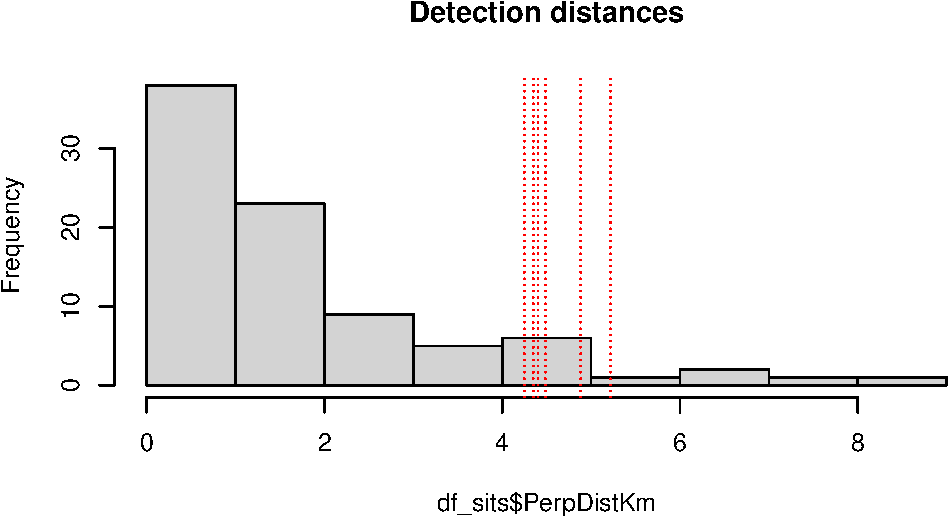
\includegraphics{figures/unnamed-chunk-280-1.pdf}

Get sample size remaining for each candidate distance:

\begin{Shaded}
\begin{Highlighting}[]
\FunctionTok{data.frame}\NormalTok{(}\AttributeTok{km =}\NormalTok{ truncation\_options, }
           \AttributeTok{n =} \FunctionTok{sapply}\NormalTok{(truncation\_options, }
                      \ControlFlowTok{function}\NormalTok{(x)\{}\FunctionTok{length}\NormalTok{(}\FunctionTok{which}\NormalTok{(df\_sits}\SpecialCharTok{$}\NormalTok{PerpDistKm }\SpecialCharTok{\textless{}=}\NormalTok{ x))\}))}
\NormalTok{          km  n}
\DecValTok{90}\NormalTok{\% }\FloatTok{4.249637} \DecValTok{77}
\DecValTok{91}\NormalTok{\% }\FloatTok{4.350266} \DecValTok{78}
\DecValTok{92}\NormalTok{\% }\FloatTok{4.403387} \DecValTok{79}
\DecValTok{93}\NormalTok{\% }\FloatTok{4.486396} \DecValTok{80}
\DecValTok{94}\NormalTok{\% }\FloatTok{4.881672} \DecValTok{80}
\DecValTok{95}\NormalTok{\% }\FloatTok{5.217843} \DecValTok{81}
\end{Highlighting}
\end{Shaded}

Based on these results, we will choose a truncation distance of 4.5 km.

\begin{Shaded}
\begin{Highlighting}[]
\NormalTok{truncation\_distance }\OtherTok{\textless{}{-}} \FloatTok{4.5}
\end{Highlighting}
\end{Shaded}

\hypertarget{ss}{%
\subsection*{\texorpdfstring{\texttt{ss}}{ss}}\label{ss}}
\addcontentsline{toc}{subsection}{\texttt{ss}}

This is a numeric vector of subgroup school sizes. The function will find this vector's geometric mean and bootstrapped CV. In Bradford et al.~(2020), school size data come from all Phase 1 and Phase 2 estimates of subgroup sizes from 2010 onwards. In the processed \texttt{cruz} object, each of those estimates is the geometric mean of repeat estimates from separate observers.

\begin{Shaded}
\begin{Highlighting}[]
\NormalTok{ss  }\OtherTok{\textless{}{-}}
\NormalTok{  cruz}\SpecialCharTok{$}\NormalTok{cohort}\SpecialCharTok{$}\NormalTok{all}\SpecialCharTok{$}\NormalTok{subgroups}\SpecialCharTok{$}\NormalTok{subgroups }\SpecialCharTok{\%\textgreater{}\%}
  \FunctionTok{filter}\NormalTok{(lubridate}\SpecialCharTok{::}\FunctionTok{year}\NormalTok{(DateTime) }\SpecialCharTok{\textgreater{}=} \DecValTok{2011}\NormalTok{,}
\NormalTok{         Lat }\SpecialCharTok{\textgreater{}=} \DecValTok{5}\NormalTok{, Lat }\SpecialCharTok{\textless{}=} \DecValTok{40}\NormalTok{, Lon }\SpecialCharTok{\textgreater{}=} \SpecialCharTok{{-}}\DecValTok{185}\NormalTok{, Lon }\SpecialCharTok{\textless{}=} \SpecialCharTok{{-}}\DecValTok{120}\NormalTok{,}
\NormalTok{         Species }\SpecialCharTok{==} \StringTok{\textquotesingle{}033\textquotesingle{}}\NormalTok{) }\SpecialCharTok{\%\textgreater{}\%}
  \FunctionTok{pull}\NormalTok{(GSBest\_geom)}
  
\NormalTok{ss }\SpecialCharTok{\%\textgreater{}\%}\NormalTok{ length}
\NormalTok{[}\DecValTok{1}\NormalTok{] }\DecValTok{183}

\NormalTok{ss}
\NormalTok{  [}\DecValTok{1}\NormalTok{]  }\FloatTok{5.00}  \FloatTok{7.00}  \FloatTok{1.00}  \FloatTok{1.00}  \FloatTok{1.00}  \FloatTok{1.33}  \FloatTok{2.00}  \FloatTok{2.75}  \FloatTok{2.67}  \FloatTok{1.00}  \FloatTok{6.00}  \FloatTok{1.00}
\NormalTok{ [}\DecValTok{13}\NormalTok{]  }\FloatTok{2.00} \FloatTok{18.50}  \FloatTok{1.00}  \FloatTok{4.00}  \FloatTok{5.00}  \FloatTok{2.00}  \FloatTok{1.00}  \FloatTok{4.00}  \FloatTok{4.50}  \FloatTok{2.50}  \FloatTok{2.00}  \FloatTok{2.00}
\NormalTok{ [}\DecValTok{25}\NormalTok{]  }\FloatTok{1.00}  \FloatTok{1.00}  \FloatTok{5.00}  \FloatTok{1.00}  \FloatTok{4.00}  \FloatTok{1.00}  \FloatTok{1.00}  \FloatTok{1.00}  \FloatTok{1.00}  \FloatTok{1.00}  \FloatTok{1.00}  \FloatTok{2.00}
\NormalTok{ [}\DecValTok{37}\NormalTok{]  }\FloatTok{2.00}  \FloatTok{1.00}  \FloatTok{4.00}  \FloatTok{9.83}  \FloatTok{2.50}  \FloatTok{4.75}  \FloatTok{8.25}  \FloatTok{3.00}  \FloatTok{2.00}  \FloatTok{3.00}  \FloatTok{3.67}  \FloatTok{3.50}
\NormalTok{ [}\DecValTok{49}\NormalTok{]  }\FloatTok{4.50}  \FloatTok{2.00}  \FloatTok{1.00}  \FloatTok{1.00}  \FloatTok{2.00}  \FloatTok{1.00}  \FloatTok{1.00}  \FloatTok{1.00}  \FloatTok{1.00}  \FloatTok{1.00}  \FloatTok{2.00}  \FloatTok{1.00}
\NormalTok{ [}\DecValTok{61}\NormalTok{]  }\FloatTok{1.00}  \FloatTok{1.00}  \FloatTok{2.00}  \FloatTok{3.00}  \FloatTok{2.00}  \FloatTok{1.50}  \FloatTok{2.67}  \FloatTok{1.33}  \FloatTok{2.00}  \FloatTok{6.00}  \FloatTok{4.33}  \FloatTok{2.00}
\NormalTok{ [}\DecValTok{73}\NormalTok{]  }\FloatTok{1.00}  \FloatTok{3.00}  \FloatTok{5.00}  \FloatTok{5.80}  \FloatTok{4.00}  \FloatTok{1.00}  \FloatTok{2.00}  \FloatTok{2.00}  \FloatTok{4.00}  \FloatTok{4.50}  \FloatTok{2.00}  \FloatTok{2.00}
\NormalTok{ [}\DecValTok{85}\NormalTok{]  }\FloatTok{2.00}  \FloatTok{4.50}  \FloatTok{2.00}  \FloatTok{1.00}  \FloatTok{2.00}  \FloatTok{1.00}  \FloatTok{1.00}  \FloatTok{2.00}  \FloatTok{2.00}  \FloatTok{1.50}  \FloatTok{4.50}  \FloatTok{1.00}
\NormalTok{ [}\DecValTok{97}\NormalTok{]  }\FloatTok{1.00}  \FloatTok{3.33}  \FloatTok{3.00}  \FloatTok{2.00}  \FloatTok{2.00}  \FloatTok{7.50}  \FloatTok{5.00}  \FloatTok{4.00}  \FloatTok{3.67}  \FloatTok{2.00}  \FloatTok{3.00}  \FloatTok{2.00}
\NormalTok{[}\DecValTok{109}\NormalTok{]  }\FloatTok{8.50}  \FloatTok{8.00}  \FloatTok{4.00}  \FloatTok{2.00}  \FloatTok{1.00}  \FloatTok{1.00}  \FloatTok{4.00}  \FloatTok{4.00}  \FloatTok{2.00}  \FloatTok{1.00}  \FloatTok{2.00}  \FloatTok{6.00}
\NormalTok{[}\DecValTok{121}\NormalTok{]  }\FloatTok{2.00}  \FloatTok{2.00}  \FloatTok{2.50}  \FloatTok{1.00}  \FloatTok{1.00}  \FloatTok{1.00}  \FloatTok{1.00}  \FloatTok{1.00}  \FloatTok{2.00}  \FloatTok{2.00}  \FloatTok{1.00}  \FloatTok{1.00}
\NormalTok{[}\DecValTok{133}\NormalTok{]  }\FloatTok{1.00}  \FloatTok{1.00}  \FloatTok{1.00}  \FloatTok{1.00}  \FloatTok{1.00}  \FloatTok{2.00}  \FloatTok{1.00}  \FloatTok{2.00}  \FloatTok{2.00}  \FloatTok{2.00}  \FloatTok{1.00}  \FloatTok{4.00}
\NormalTok{[}\DecValTok{145}\NormalTok{]  }\FloatTok{7.50}  \FloatTok{1.50}  \FloatTok{2.00}  \FloatTok{1.00}  \FloatTok{1.00}  \FloatTok{1.00}  \FloatTok{1.00}  \FloatTok{2.00}  \FloatTok{1.00}  \FloatTok{2.00}  \FloatTok{3.00}  \FloatTok{3.00}
\NormalTok{[}\DecValTok{157}\NormalTok{]  }\FloatTok{2.00}  \FloatTok{3.00}  \FloatTok{1.50}  \FloatTok{1.00}  \FloatTok{1.00}  \FloatTok{3.00}  \FloatTok{2.00}  \FloatTok{4.00}  \FloatTok{1.00}  \FloatTok{1.00}  \FloatTok{1.00}  \FloatTok{2.00}
\NormalTok{[}\DecValTok{169}\NormalTok{]  }\FloatTok{2.00}  \FloatTok{4.00}  \FloatTok{2.00}  \FloatTok{2.00}  \FloatTok{1.00}  \FloatTok{1.00}  \FloatTok{3.00}  \FloatTok{1.00}  \FloatTok{3.00}  \FloatTok{2.50}  \FloatTok{2.00}  \FloatTok{2.00}
\NormalTok{[}\DecValTok{181}\NormalTok{]  }\FloatTok{1.00}  \FloatTok{1.00}  \FloatTok{1.00}
\end{Highlighting}
\end{Shaded}

\hypertarget{cruz10}{%
\subsection*{\texorpdfstring{\texttt{cruz10}}{cruz10}}\label{cruz10}}
\addcontentsline{toc}{subsection}{\texttt{cruz10}}

This is a processed \texttt{cruz} object with short segment lengths, ideally 10 km or less (hence the 10 in the input name). This \texttt{cruz} object will be used to estimate \emph{Rg(0)}, i.e., the relative trackline detection probability (see its chapter). \texttt{LTabundR} comes with a built-in dataset we can use for this purpose:

\begin{Shaded}
\begin{Highlighting}[]
\FunctionTok{data}\NormalTok{(}\StringTok{"noaa\_10km\_1986\_2020"}\NormalTok{)}
\NormalTok{cruz10 }\OtherTok{\textless{}{-}}\NormalTok{ noaa\_10km\_1986\_2020}
\end{Highlighting}
\end{Shaded}

The code used to generate this dataset can be seen by pulling up the help documentation: \texttt{?noaa\_10km\_1986\_2020}.

\hypertarget{g0_spp}{%
\subsection*{\texorpdfstring{\texttt{g0\_spp}}{g0\_spp}}\label{g0_spp}}
\addcontentsline{toc}{subsection}{\texttt{g0\_spp}}

This is a character vector of species code(s) to use to estimate \emph{Rg(0)}. In most cases this will be a single species, e.g., \texttt{"033"} for false killer whales.

\begin{Shaded}
\begin{Highlighting}[]
\NormalTok{g0\_spp }\OtherTok{\textless{}{-}} \StringTok{\textquotesingle{}033\textquotesingle{}}
\end{Highlighting}
\end{Shaded}

\hypertarget{g0_truncation}{%
\subsection*{\texorpdfstring{\texttt{g0\_truncation}}{g0\_truncation}}\label{g0_truncation}}
\addcontentsline{toc}{subsection}{\texttt{g0\_truncation}}

The truncation distance to use when estimating Rg(0). In Bradford et al.~(2020) this is 5.5 km.

\begin{Shaded}
\begin{Highlighting}[]
\NormalTok{g0\_truncation }\OtherTok{\textless{}{-}} \FloatTok{5.5}
\end{Highlighting}
\end{Shaded}

\hypertarget{g0_pool_bft}{%
\subsection*{\texorpdfstring{\texttt{g0\_pool\_bft}}{g0\_pool\_bft}}\label{g0_pool_bft}}
\addcontentsline{toc}{subsection}{\texttt{g0\_pool\_bft}}

A way to specify that low Beaufort sea states, which are typically rare in open-ocean surveys, should be pooled. This step may be needed in order to achieve a monotonic decline in the \emph{g(0)} \textasciitilde{} Bft relationship, but the default is \texttt{NULL}, i.e., no pooling. If \texttt{g0\_pool\_bft} is the character string \texttt{"01"}, Beaufort states 1 will be pooled into state 0. If \texttt{g0\_pool\_bft} is the character string \texttt{"012"}, Beaufort states 1 and 2 will be pooled into state 0.

\begin{Shaded}
\begin{Highlighting}[]
\NormalTok{g0\_pool\_bft }\OtherTok{=} \ConstantTok{NULL}
\end{Highlighting}
\end{Shaded}

\hypertarget{g0_jackknife_fraction}{%
\subsection*{\texorpdfstring{\texttt{g0\_jackknife\_fraction}}{g0\_jackknife\_fraction}}\label{g0_jackknife_fraction}}
\addcontentsline{toc}{subsection}{\texttt{g0\_jackknife\_fraction}}

The proportion of data to leave out within each jackknife permutation. The default is \texttt{0.1} (i.e., 10\% of the data, yielding 10 jackknife loops), after Barlow (2015).

\begin{Shaded}
\begin{Highlighting}[]
\NormalTok{g0\_jackknife\_fraction }\OtherTok{=} \FloatTok{0.1}
\end{Highlighting}
\end{Shaded}

\hypertarget{density_segments}{%
\subsection*{\texorpdfstring{\texttt{density\_segments}}{density\_segments}}\label{density_segments}}
\addcontentsline{toc}{subsection}{\texttt{density\_segments}}

The survey segments to be used in density/abundance estimation. For example, Bradford et al.~(2020) used 150-km segments to estimate false killer whale density in the Hawaiian EEZ in 2017. For this we can use the 1986-2020 dataset we loaded above. Note that no filtering will be applied to these segments by the \texttt{lta\_subgroup()} function, so w need to filter them ourselves first: we want only systematic segments for the Hawaiian EEZ in 2017 (specially, just cruises 1705 and 1706).

\begin{Shaded}
\begin{Highlighting}[]
\NormalTok{cruzi }\OtherTok{\textless{}{-}} \FunctionTok{filter\_cruz}\NormalTok{(}\AttributeTok{cruz =}\NormalTok{ cruz,}
                      \AttributeTok{analysis\_only =} \ConstantTok{TRUE}\NormalTok{,}
                      \AttributeTok{years =} \DecValTok{2017}\NormalTok{,}
                      \AttributeTok{cruises =} \FunctionTok{c}\NormalTok{(}\DecValTok{1705}\NormalTok{, }\DecValTok{1706}\NormalTok{),}
                      \AttributeTok{regions =} \StringTok{\textquotesingle{}HI\_EEZ\textquotesingle{}}\NormalTok{,}
                      \AttributeTok{bft\_range =} \DecValTok{0}\SpecialCharTok{:}\DecValTok{6}\NormalTok{,}
                      \AttributeTok{eff\_types =} \StringTok{\textquotesingle{}S\textquotesingle{}}\NormalTok{,}
                      \AttributeTok{on\_off =} \ConstantTok{TRUE}\NormalTok{)}
\end{Highlighting}
\end{Shaded}

From this filtered cruz object, we will isolate the segments data:

\begin{Shaded}
\begin{Highlighting}[]
\NormalTok{density\_segments }\OtherTok{\textless{}{-}}\NormalTok{ cruzi}\SpecialCharTok{$}\NormalTok{cohorts}\SpecialCharTok{$}\NormalTok{all}\SpecialCharTok{$}\NormalTok{segments}
\end{Highlighting}
\end{Shaded}

Since we do not want to stratify our analysis by smaller geostrata, such as the Main Hawaiian Islands, we will go ahead and coerce all stratum assignments to the Hawaiian EEZ geostratum:

\begin{Shaded}
\begin{Highlighting}[]
\NormalTok{density\_segments}\SpecialCharTok{$}\NormalTok{stratum }\OtherTok{\textless{}{-}} \StringTok{\textquotesingle{}HI\_EEZ\textquotesingle{}}
\end{Highlighting}
\end{Shaded}

\hypertarget{density_das}{%
\subsection*{\texorpdfstring{\texttt{density\_das}}{density\_das}}\label{density_das}}
\addcontentsline{toc}{subsection}{\texttt{density\_das}}

This is the complete survey data corresponding to the above segments. These data will be used to determine the proportion of survey effort occurring in each Beaufort sea state during estimation of \emph{Relative g(0)}.

\begin{Shaded}
\begin{Highlighting}[]
\NormalTok{density\_das }\OtherTok{\textless{}{-}}\NormalTok{ cruzi}\SpecialCharTok{$}\NormalTok{cohorts}\SpecialCharTok{$}\NormalTok{all}\SpecialCharTok{$}\NormalTok{das}
\end{Highlighting}
\end{Shaded}

\hypertarget{density_sightings}{%
\subsection*{\texorpdfstring{\texttt{density\_sightings}}{density\_sightings}}\label{density_sightings}}
\addcontentsline{toc}{subsection}{\texttt{density\_sightings}}

These are the encounters to use in density/abundance estimation. In Bradford et al.~(20120), these were the Phase 1 detections of false killer whale subgroups within the population-region-year of interest, e.g., Northwest Hawaiian Island population sightings within the Hawaiian EEZ in 2017. No filtering is applied to these sightings within \texttt{lta\_subgroups()}, so make sure only the sightings you wish to use are included and nothing more.

In this example, since we do not have population information on hand, we will not filter detections to a specific population. Instead, we will estimate abundance of all false killer whales within the Hawaiian EEZ:

\begin{Shaded}
\begin{Highlighting}[]
\NormalTok{density\_sightings  }\OtherTok{\textless{}{-}}
\NormalTok{  cruz}\SpecialCharTok{$}\NormalTok{cohorts}\SpecialCharTok{$}\NormalTok{all}\SpecialCharTok{$}\NormalTok{subgroups}\SpecialCharTok{$}\NormalTok{subgroups }\SpecialCharTok{\%\textgreater{}\%}
  \FunctionTok{filter}\NormalTok{(EffType }\SpecialCharTok{==} \StringTok{\textquotesingle{}S\textquotesingle{}}\NormalTok{,}
\NormalTok{         OnEffort }\SpecialCharTok{==} \ConstantTok{TRUE}\NormalTok{,}
\NormalTok{         lubridate}\SpecialCharTok{::}\FunctionTok{year}\NormalTok{(DateTime) }\SpecialCharTok{==} \DecValTok{2017}\NormalTok{,}
\NormalTok{         PerpDist }\SpecialCharTok{\textless{}=}\NormalTok{ truncation\_distance,}
\NormalTok{         Species }\SpecialCharTok{==} \StringTok{\textquotesingle{}033\textquotesingle{}}\NormalTok{,}
\NormalTok{         Phase }\SpecialCharTok{==} \DecValTok{1}\NormalTok{)}

\NormalTok{density\_sightings }\SpecialCharTok{\%\textgreater{}\%}\NormalTok{ nrow}
\NormalTok{[}\DecValTok{1}\NormalTok{] }\DecValTok{32}

\NormalTok{density\_sightings }\SpecialCharTok{\%\textgreater{}\%}\NormalTok{ head}
\NormalTok{  Cruise       Date            DateTime      Lat       Lon OnEffort Bft EffType}
\DecValTok{1}   \DecValTok{1705} \DecValTok{2017{-}09{-}21} \DecValTok{2017{-}09{-}21} \DecValTok{14}\SpecialCharTok{:}\DecValTok{17}\SpecialCharTok{:}\DecValTok{27} \FloatTok{20.04283} \SpecialCharTok{{-}}\FloatTok{161.9177}     \ConstantTok{TRUE}   \DecValTok{5}\NormalTok{       S}
\DecValTok{2}   \DecValTok{1705} \DecValTok{2017{-}09{-}21} \DecValTok{2017{-}09{-}21} \DecValTok{14}\SpecialCharTok{:}\DecValTok{39}\SpecialCharTok{:}\DecValTok{40} \FloatTok{20.06017} \SpecialCharTok{{-}}\FloatTok{161.9840}     \ConstantTok{TRUE}   \DecValTok{5}\NormalTok{       S}
\DecValTok{3}   \DecValTok{1705} \DecValTok{2017{-}09{-}29} \DecValTok{2017{-}09{-}29} \DecValTok{13}\SpecialCharTok{:}\DecValTok{22}\SpecialCharTok{:}\DecValTok{08} \FloatTok{23.55750} \SpecialCharTok{{-}}\FloatTok{175.8527}     \ConstantTok{TRUE}   \DecValTok{1}\NormalTok{       S}
\DecValTok{4}   \DecValTok{1705} \DecValTok{2017{-}09{-}29} \DecValTok{2017{-}09{-}29} \DecValTok{13}\SpecialCharTok{:}\DecValTok{26}\SpecialCharTok{:}\DecValTok{05} \FloatTok{23.56050} \SpecialCharTok{{-}}\FloatTok{175.8643}     \ConstantTok{TRUE}   \DecValTok{1}\NormalTok{       S}
\DecValTok{5}   \DecValTok{1705} \DecValTok{2017{-}09{-}29} \DecValTok{2017{-}09{-}29} \DecValTok{13}\SpecialCharTok{:}\DecValTok{26}\SpecialCharTok{:}\DecValTok{43} \FloatTok{23.56083} \SpecialCharTok{{-}}\FloatTok{175.8662}     \ConstantTok{TRUE}   \DecValTok{1}\NormalTok{       S}
\DecValTok{6}   \DecValTok{1705} \DecValTok{2017{-}09{-}29} \DecValTok{2017{-}09{-}29} \DecValTok{13}\SpecialCharTok{:}\DecValTok{32}\SpecialCharTok{:}\DecValTok{33} \FloatTok{23.56517} \SpecialCharTok{{-}}\FloatTok{175.8832}     \ConstantTok{TRUE}   \DecValTok{1}\NormalTok{       S}
\NormalTok{  SightNo Species SubGrp Angle   RadDist seg\_id  PerpDist GSBest GSH  GSL}
\DecValTok{1}     \DecValTok{064}     \DecValTok{033}\NormalTok{      A    }\DecValTok{14} \FloatTok{5.0374102}   \DecValTok{1602} \FloatTok{1.2186598}   \FloatTok{3.00}   \DecValTok{4} \FloatTok{2.00}
\DecValTok{2}     \DecValTok{064}     \DecValTok{033}\NormalTok{      B    }\DecValTok{24} \FloatTok{3.1483814}   \DecValTok{1602} \FloatTok{1.2805621}   \FloatTok{3.67}   \DecValTok{6} \FloatTok{2.33}
\DecValTok{3}     \DecValTok{073}     \DecValTok{033}\NormalTok{      A    }\DecValTok{49} \FloatTok{3.3706200}   \DecValTok{1610} \FloatTok{2.5438392}   \FloatTok{2.00}   \DecValTok{3} \FloatTok{1.00}
\DecValTok{4}     \DecValTok{073}     \DecValTok{033}\NormalTok{      B    }\DecValTok{68} \FloatTok{0.6852359}   \DecValTok{1610} \FloatTok{0.6353397}   \FloatTok{1.00}   \DecValTok{2} \FloatTok{1.00}
\DecValTok{5}     \DecValTok{073}     \DecValTok{033}\NormalTok{      C    }\DecValTok{40} \FloatTok{0.3703978}   \DecValTok{1610} \FloatTok{0.2380871}   \FloatTok{1.00}   \DecValTok{1} \FloatTok{1.00}
\DecValTok{6}     \DecValTok{073}     \DecValTok{033}\NormalTok{      E    }\DecValTok{89} \FloatTok{2.9817023}   \DecValTok{1610} \FloatTok{2.9812482}   \FloatTok{1.00}   \DecValTok{2} \FloatTok{1.00}
\NormalTok{  GSBest\_geom GSH\_geom GSL\_geom  use stratum\_HI\_EEZ stratum\_OtherCNP}
\DecValTok{1}        \FloatTok{3.00}        \DecValTok{4}     \FloatTok{2.00} \ConstantTok{TRUE}           \ConstantTok{TRUE}             \ConstantTok{TRUE}
\DecValTok{2}        \FloatTok{3.67}        \DecValTok{6}     \FloatTok{2.33} \ConstantTok{TRUE}           \ConstantTok{TRUE}             \ConstantTok{TRUE}
\DecValTok{3}        \FloatTok{2.00}        \DecValTok{3}     \FloatTok{1.00} \ConstantTok{TRUE}           \ConstantTok{TRUE}             \ConstantTok{TRUE}
\DecValTok{4}        \FloatTok{1.00}        \DecValTok{2}     \FloatTok{1.00} \ConstantTok{TRUE}           \ConstantTok{TRUE}             \ConstantTok{TRUE}
\DecValTok{5}        \FloatTok{1.00}        \DecValTok{1}     \FloatTok{1.00} \ConstantTok{TRUE}           \ConstantTok{TRUE}             \ConstantTok{TRUE}
\DecValTok{6}        \FloatTok{1.00}        \DecValTok{2}     \FloatTok{1.00} \ConstantTok{TRUE}           \ConstantTok{TRUE}             \ConstantTok{TRUE}
\NormalTok{  stratum\_MHI stratum Phase}
\DecValTok{1}       \ConstantTok{FALSE}\NormalTok{  HI\_EEZ     }\DecValTok{1}
\DecValTok{2}       \ConstantTok{FALSE}\NormalTok{  HI\_EEZ     }\DecValTok{1}
\DecValTok{3}       \ConstantTok{FALSE}\NormalTok{  HI\_EEZ     }\DecValTok{1}
\DecValTok{4}       \ConstantTok{FALSE}\NormalTok{  HI\_EEZ     }\DecValTok{1}
\DecValTok{5}       \ConstantTok{FALSE}\NormalTok{  HI\_EEZ     }\DecValTok{1}
\DecValTok{6}       \ConstantTok{FALSE}\NormalTok{  HI\_EEZ     }\DecValTok{1}
\end{Highlighting}
\end{Shaded}

As above, let's make sure the geostratum assignments for these sightings are simple:

\begin{Shaded}
\begin{Highlighting}[]
\NormalTok{density\_segments}\SpecialCharTok{$}\NormalTok{stratum }\OtherTok{\textless{}{-}} \StringTok{\textquotesingle{}HI\_EEZ\textquotesingle{}}
\end{Highlighting}
\end{Shaded}

\hypertarget{abundance_area}{%
\subsection*{\texorpdfstring{\texttt{abundance\_area}}{abundance\_area}}\label{abundance_area}}
\addcontentsline{toc}{subsection}{\texttt{abundance\_area}}

This is the area, in square km, of the region of interest. The density estimate will be scaled by this area.

We have two options for finding this area. The first is to draw the area from our \texttt{cohort\$strata} slot:

\begin{Shaded}
\begin{Highlighting}[]
\NormalTok{cruz}\SpecialCharTok{$}\NormalTok{strata}\SpecialCharTok{$}\NormalTok{area[cruz}\SpecialCharTok{$}\NormalTok{strata}\SpecialCharTok{$}\NormalTok{stratum }\SpecialCharTok{==} \StringTok{\textquotesingle{}HI\_EEZ\textquotesingle{}}\NormalTok{]}
\NormalTok{[}\DecValTok{1}\NormalTok{] }\DecValTok{2474596}
\end{Highlighting}
\end{Shaded}

The second is to calculate it ourselves using the \texttt{LTabundR} function \texttt{strata\_area()}. This second option will be useful if your study area is a complicated combination/substraction of multiple geostrata.

\begin{Shaded}
\begin{Highlighting}[]
\FunctionTok{data}\NormalTok{(strata\_cnp)}

\NormalTok{abundance\_area }\OtherTok{\textless{}{-}} 
  \FunctionTok{strata\_area}\NormalTok{(}\AttributeTok{strata\_all =}\NormalTok{ strata\_cnp,}
              \AttributeTok{strata\_keep =} \StringTok{\textquotesingle{}HI\_EEZ\textquotesingle{}}\NormalTok{)}\SpecialCharTok{$}\NormalTok{km2}
\end{Highlighting}
\end{Shaded}

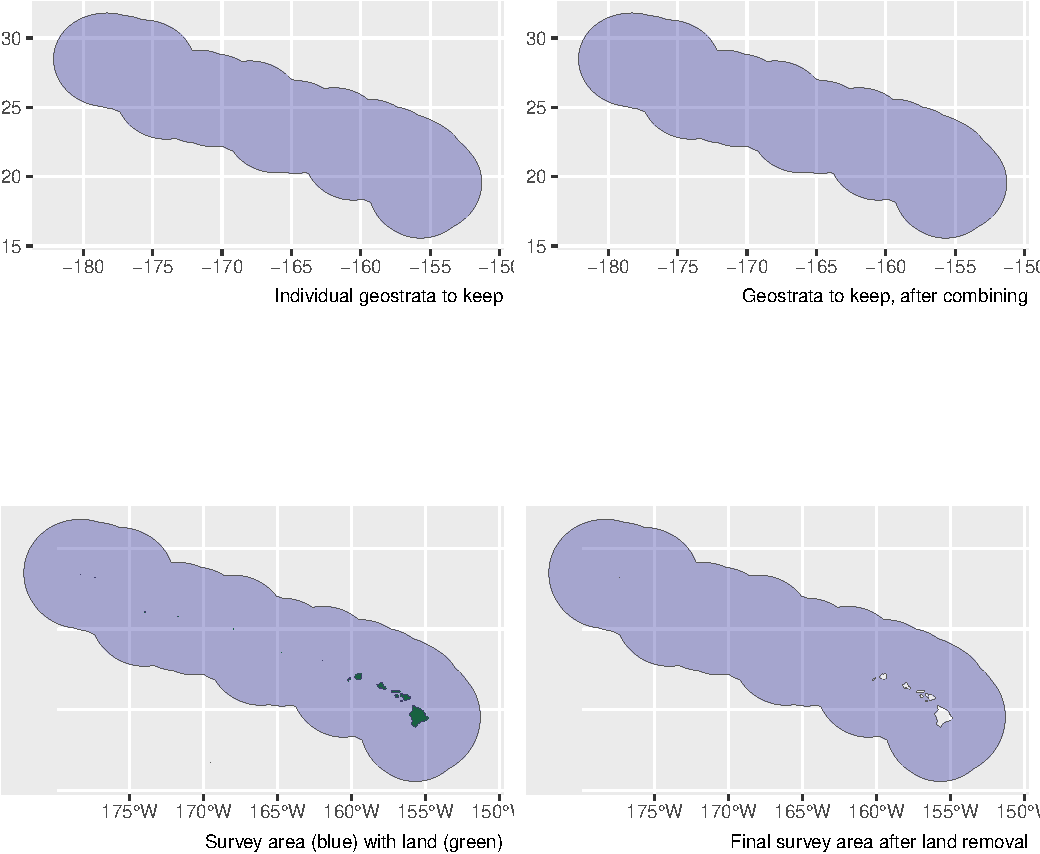
\includegraphics{figures/unnamed-chunk-296-1.pdf}

\begin{Shaded}
\begin{Highlighting}[]

\NormalTok{abundance\_area}
\NormalTok{[}\DecValTok{1}\NormalTok{] }\DecValTok{2474596}
\end{Highlighting}
\end{Shaded}

\hypertarget{remaining-inputs}{%
\subsection*{Remaining inputs}\label{remaining-inputs}}
\addcontentsline{toc}{subsection}{Remaining inputs}

\textbf{\texttt{iterations}}: Number of iterations to use in the various CV bootstrapping procedures occurring throughout this function, specifically: Effective Strip Half-Width CV estimation, school size CV estimation, weighted g(0) CV estimation, and encounter rate estimation.

\textbf{\texttt{output\_dir}}: The path in which results RData files should be stored. If left ``\,``, the current working directory will be used.

\textbf{\texttt{toplot}}: A Boolean, with default FALSE, indicating whether to plot various aspects of the analysis.

\textbf{\texttt{verbose}}: A Boolean, with default TRUE, indicating whether to print status updates to the Console.

\textbf{\texttt{density\_bootstraps}}: Number of bootstrap iterations to use for the CV estimate of density and abundance specifically. This input allows this final step to use a different (typically larger) iteration size than the iterations input above.

\begin{Shaded}
\begin{Highlighting}[]
\FunctionTok{save}\NormalTok{(results\_subgroup, }\AttributeTok{file=}\StringTok{\textquotesingle{}results\_subgroup.RData\textquotesingle{}}\NormalTok{)}
\end{Highlighting}
\end{Shaded}

\begin{Shaded}
\begin{Highlighting}[]
\FunctionTok{load}\NormalTok{(}\StringTok{\textquotesingle{}results\_subgroup.RData\textquotesingle{}}\NormalTok{)}
\end{Highlighting}
\end{Shaded}

\hypertarget{outputs-1}{%
\section*{Outputs}\label{outputs-1}}
\addcontentsline{toc}{section}{Outputs}

The function returns a \texttt{list} with many slots, including estimates of density and abundance -- along with estimates of intermediate parameters -- with a CV derived from a bootstrapping routine. To demonstrate this output, we will use results from a call with only 10 bootstrap iterations.

\begin{Shaded}
\begin{Highlighting}[]
\NormalTok{results\_subgroup }\SpecialCharTok{\%\textgreater{}\%}\NormalTok{ names}
\NormalTok{ [}\DecValTok{1}\NormalTok{] }\StringTok{"D"}                  \StringTok{"D\_CV"}               \StringTok{"D\_L95"}             
\NormalTok{ [}\DecValTok{4}\NormalTok{] }\StringTok{"D\_U95"}              \StringTok{"N"}                  \StringTok{"N\_CV"}              
\NormalTok{ [}\DecValTok{7}\NormalTok{] }\StringTok{"N\_L95"}              \StringTok{"N\_U95"}              \StringTok{"ER"}                
\NormalTok{[}\DecValTok{10}\NormalTok{] }\StringTok{"ss"}                 \StringTok{"n"}                  \StringTok{"L"}                 
\NormalTok{[}\DecValTok{13}\NormalTok{] }\StringTok{"n\_segments"}         \StringTok{"g0"}                 \StringTok{"g0\_cv"}             
\NormalTok{[}\DecValTok{16}\NormalTok{] }\StringTok{"g0\_details"}         \StringTok{"df"}                 \StringTok{"bootstraps"}        
\NormalTok{[}\DecValTok{19}\NormalTok{] }\StringTok{"iterations"}         \StringTok{"density\_bootstraps"}
\end{Highlighting}
\end{Shaded}

Most of these slots hold best-estimates of parameters or sample size details:

\begin{Shaded}
\begin{Highlighting}[]
\NormalTok{results\_subgroup[}\FunctionTok{c}\NormalTok{(}\DecValTok{1}\SpecialCharTok{:}\DecValTok{15}\NormalTok{, }\DecValTok{19}\SpecialCharTok{:}\DecValTok{20}\NormalTok{)]}
\SpecialCharTok{$}\NormalTok{D}
          \DecValTok{1} 
\FloatTok{0.001663263} 

\SpecialCharTok{$}\NormalTok{D\_CV}
       \DecValTok{1} 
\FloatTok{1.344861} 

\SpecialCharTok{$}\NormalTok{D\_L95}
\NormalTok{[}\DecValTok{1}\NormalTok{] }\FloatTok{0.0005004478}

\SpecialCharTok{$}\NormalTok{D\_U95}
\NormalTok{[}\DecValTok{1}\NormalTok{] }\FloatTok{0.01547307}

\SpecialCharTok{$}\NormalTok{N}
\NormalTok{[}\DecValTok{1}\NormalTok{] }\DecValTok{4116}

\SpecialCharTok{$}\NormalTok{N\_CV}
\NormalTok{[}\DecValTok{1}\NormalTok{] }\FloatTok{1.344829}

\SpecialCharTok{$}\NormalTok{N\_L95}
\NormalTok{[}\DecValTok{1}\NormalTok{] }\FloatTok{1238.357}

\SpecialCharTok{$}\NormalTok{N\_U95}
\NormalTok{[}\DecValTok{1}\NormalTok{] }\DecValTok{38290}

\SpecialCharTok{$}\NormalTok{ER}
\NormalTok{[}\DecValTok{1}\NormalTok{] }\FloatTok{0.001860071}

\SpecialCharTok{$}\NormalTok{ss}
\NormalTok{[}\DecValTok{1}\NormalTok{] }\FloatTok{2.466557}

\SpecialCharTok{$}\NormalTok{n}
\NormalTok{[}\DecValTok{1}\NormalTok{] }\DecValTok{32}

\SpecialCharTok{$}\NormalTok{L}
\NormalTok{[}\DecValTok{1}\NormalTok{] }\FloatTok{17203.64}

\SpecialCharTok{$}\NormalTok{n\_segments}
\NormalTok{[}\DecValTok{1}\NormalTok{] }\DecValTok{136}

\SpecialCharTok{$}\NormalTok{g0}
\NormalTok{[}\DecValTok{1}\NormalTok{] }\FloatTok{0.571}

\SpecialCharTok{$}\NormalTok{g0\_cv}
\NormalTok{[}\DecValTok{1}\NormalTok{] }\FloatTok{0.365}

\SpecialCharTok{$}\NormalTok{iterations}
\NormalTok{[}\DecValTok{1}\NormalTok{] }\DecValTok{10}

\SpecialCharTok{$}\NormalTok{density\_bootstraps}
\NormalTok{[}\DecValTok{1}\NormalTok{] }\DecValTok{10000}
\end{Highlighting}
\end{Shaded}

The \texttt{g0\_details} slot includes the results from the \texttt{g0\_model()} and \texttt{g0\_weighted()} functions called internally by \texttt{lta\_subgroup()}. See those functions' documentation pages for details.

\begin{Shaded}
\begin{Highlighting}[]
\NormalTok{results\_subgroup}\SpecialCharTok{$}\NormalTok{g0\_details }\SpecialCharTok{\%\textgreater{}\%}\NormalTok{ names}
\NormalTok{[}\DecValTok{1}\NormalTok{] }\StringTok{"Rg0"}       \StringTok{"gam"}       \StringTok{"jackknife"} \StringTok{"summary"}   \StringTok{"sightings"} \StringTok{"segments"} 
\end{Highlighting}
\end{Shaded}

The \texttt{df} slot includes details of the detection function fit. See the documentation for \texttt{df\_plot()} for details.

\begin{Shaded}
\begin{Highlighting}[]
\NormalTok{results\_subgroup}\SpecialCharTok{$}\NormalTok{df }\SpecialCharTok{\%\textgreater{}\%}\NormalTok{ names}
\NormalTok{[}\DecValTok{1}\NormalTok{] }\StringTok{"best\_models"}  \StringTok{"all\_models"}   \StringTok{"best\_objects"} \StringTok{"sightings"}   
\end{Highlighting}
\end{Shaded}

The \texttt{bootstraps} slot has the bootstrapped values for various parameters, in case they are useful for troubleshooting, subsequent analyses, and/or plotting:

\begin{Shaded}
\begin{Highlighting}[]
\NormalTok{results\_subgroup}\SpecialCharTok{$}\NormalTok{bootstraps }\SpecialCharTok{\%\textgreater{}\%}\NormalTok{ names}
\NormalTok{[}\DecValTok{1}\NormalTok{] }\StringTok{"esw"} \StringTok{"ss"}  \StringTok{"g0"}  \StringTok{"er"}  \StringTok{"D"}   \StringTok{"N"}  
\end{Highlighting}
\end{Shaded}

Some examples:

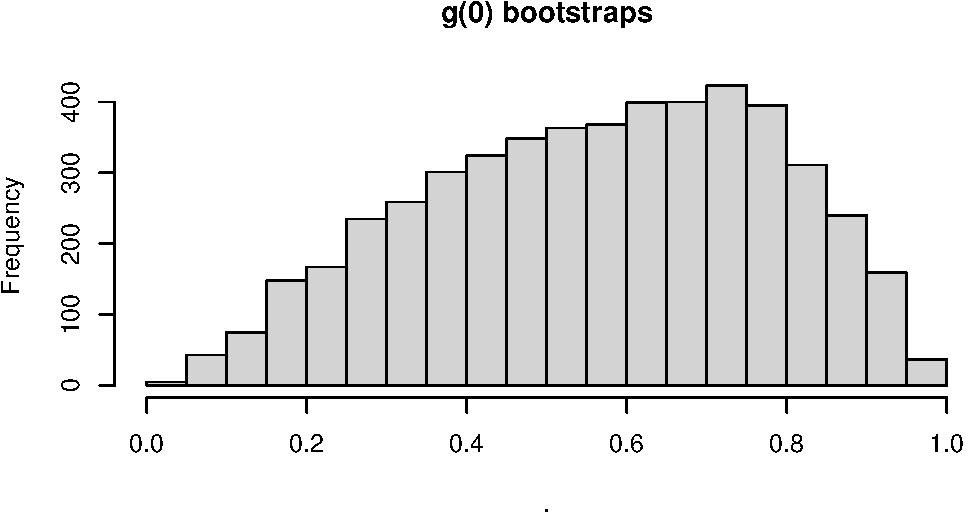
\includegraphics{figures/unnamed-chunk-305-1.pdf}

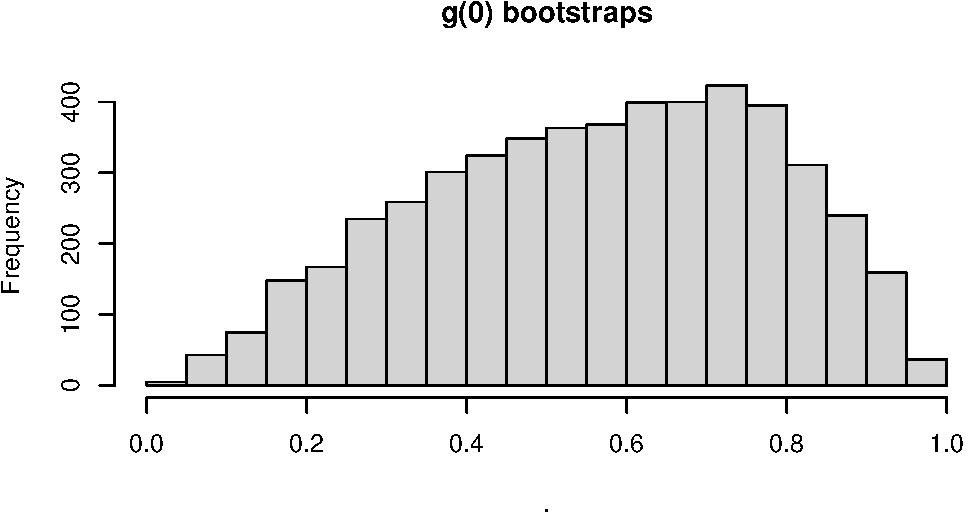
\includegraphics{figures/unnamed-chunk-306-1.pdf}

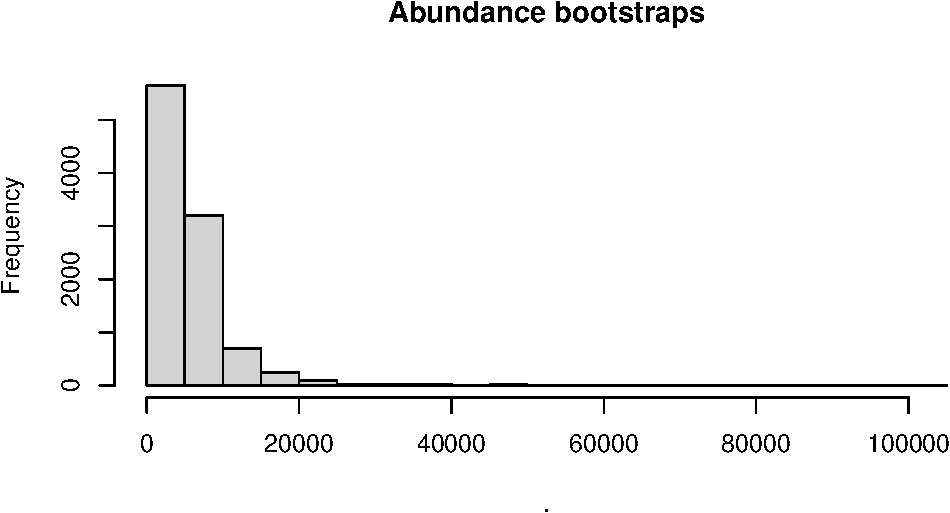
\includegraphics{figures/unnamed-chunk-307-1.pdf}

\hypertarget{behind-the-scenes-2}{%
\section*{Behind the scenes}\label{behind-the-scenes-2}}
\addcontentsline{toc}{section}{Behind the scenes}

This function performs the following operations:

\begin{enumerate}
\def\labelenumi{\arabic{enumi}.}
\item
  Fits a detection function to \texttt{df\_sits} without covariates, using the \texttt{LTabundR} function \texttt{df\_fit()}, in order to estimate the effective strip half-width (ESW).
\item
  Conducts bootstrap re-sampling of the detection function fitting routine in order to estimate the CV of ESW.
\item
  Estimates the geometric mean of subgroup school size based on the \texttt{ss} input.
\item
  Creates a bootstrap-resampled distribution of subgroup school sizes, with which CV is estimated.
\item
  Models the \emph{Relative g(0)} in different survey conditions using the \texttt{LTabundR} function \texttt{g0\_model()}. This function also estimates the CV of the \emph{Rg(0)} estimate in each Beaufort sea state using jackknife resampling.
\item
  Estimates the encounter rate (subgroup detections / trackline surveyed).
\item
  Creates a bootstrap-resampled distribution of encounter rate estimates.
\item
  Calculates a weighted \emph{g(0)} estimate according to the proportion of effort occurring in each Beaufort sea state, then uses an automated parameter optimization routine (see details in \texttt{LTabundR} function \texttt{g0\_weighted()}) to estimate the CV of the weighted \emph{g(0)} estimate.
\item
  Creates a bootstrap-resampled distribution of the weighted \emph{g(0)} estimate.
\item
  Estimates density using the best estimates of effective strip half-width, school size, \emph{g(0)}, and the encounter rate.
\item
  Estimates abundance by scaling the density estimate by the provided abundance\_area.
\item
  Creates a bootstrap-resampled distribution of the density estimate by iteratively drawing values from the resampled distributions of the constituent parameters of the density equation.
\item
  Creates a bootstrap-resampled distribtion of the abundance estimate by scaling the density distribution by abundance\_area.
\end{enumerate}

Note that this approach could theoretically be used for other species that occur in subgroups.

\hypertarget{part-results}{%
\part{Results}\label{part-results}}

\hypertarget{tables}{%
\chapter{Tables}\label{tables}}

To demonstrate how LTA results can be summarized, tabularized, and plotted, we will use a built-in \texttt{LTabundR} dataset, which has denisty/abundance estimates for the Hawaiian EEZ in 2010 and 2017 for striped dolphins, Fraser's dolphins, and melon-headed whales, ran with only 20 iterations:

\begin{Shaded}
\begin{Highlighting}[]
\FunctionTok{data}\NormalTok{(lta\_result)}
\end{Highlighting}
\end{Shaded}

We created these LTA results using the following built-in dataset:

\begin{Shaded}
\begin{Highlighting}[]
\FunctionTok{data}\NormalTok{(cnp\_150km\_1986\_2020)}
\end{Highlighting}
\end{Shaded}

\hypertarget{summary-tables}{%
\section*{Summary tables}\label{summary-tables}}
\addcontentsline{toc}{section}{Summary tables}

To summarize \texttt{lta()} results using the standard table format provided in recent NOAA stock assessment reports, use the function \texttt{lta\_report()}.

\begin{Shaded}
\begin{Highlighting}[]
\NormalTok{tables }\OtherTok{\textless{}{-}} \FunctionTok{lta\_report}\NormalTok{(lta\_result, }
                     \AttributeTok{cruz =}\NormalTok{ cnp\_150km\_1986\_2020,}
                     \AttributeTok{verbose =} \ConstantTok{TRUE}\NormalTok{)}
\end{Highlighting}
\end{Shaded}

Providing the \texttt{cruz} object is not required, but if it is not provided, one of the five summary tables (\texttt{\$table1a} below) will not be returned.

\begin{Shaded}
\begin{Highlighting}[]
\NormalTok{tables }\SpecialCharTok{\%\textgreater{}\%}\NormalTok{ names}
\NormalTok{[}\DecValTok{1}\NormalTok{] }\StringTok{"table1a"} \StringTok{"table1b"} \StringTok{"table2"}  \StringTok{"table3"}  \StringTok{"table4"}  \StringTok{"tableA1"} \StringTok{"tableA2"}
\end{Highlighting}
\end{Shaded}

\hypertarget{table-1-in-reports-sample-sizes}{%
\subsection*{Table 1 in reports: Sample sizes}\label{table-1-in-reports-sample-sizes}}
\addcontentsline{toc}{subsection}{Table 1 in reports: Sample sizes}

\hypertarget{table-1a}{%
\subsubsection*{Table 1a}\label{table-1a}}
\addcontentsline{toc}{subsubsection}{Table 1a}

If \texttt{cruz} was provided, \texttt{\$table1a} 1a will include total sighting counts for all species in the years from \texttt{lta\_result}, broken down by region. The \texttt{Ntot} column holds all sightings, regardless of effort status or Beaufort sea state. \texttt{Nsys} holds counts of systematic-only sightings (i.e., EffType = ``S'' and Bft \textless= 6), which may still include sightings that are beyond the species-specific truncation distance and were therefore excluded from density/abundance estimation.

These counts are provided separately from the \texttt{\$table1b} slot below, since those counts are based on the \texttt{lta\_result} object, and will not include sightings for species that did not have a specific LTA estimate specified when it was made. We also include this separately so as to give the user full flexibility in how they summarize sighting counts by region/population/stock.

\begin{Shaded}
\begin{Highlighting}[]
\NormalTok{tables}\SpecialCharTok{$}\NormalTok{table1a }\SpecialCharTok{\%\textgreater{}\%}
\NormalTok{  DT}\SpecialCharTok{::}\FunctionTok{datatable}\NormalTok{(}\AttributeTok{options=}\FunctionTok{list}\NormalTok{(}\AttributeTok{initComplete =}\NormalTok{ htmlwidgets}\SpecialCharTok{::}\FunctionTok{JS}\NormalTok{(}
    \StringTok{"function(settings, json) \{$(this.api().table().container()).css(\{\textquotesingle{}font{-}size\textquotesingle{}: \textquotesingle{}9pt\textquotesingle{}\});\}"}\NormalTok{)}
\NormalTok{  ))}
\end{Highlighting}
\end{Shaded}

\hypertarget{table-1b}{%
\subsubsection*{Table 1b}\label{table-1b}}
\addcontentsline{toc}{subsubsection}{Table 1b}

This table holds sighting counts used in estimates of density/abundance. The rows match the rows for Tables 3 and 4. In this table, columns are still prepared for total sightings (\texttt{Ntot}) and systematic sightings (\texttt{Nsys}), but they are left blank, since it is not clear how sightings from multiple regions in \texttt{\$table1a} would be concatenated for this table. The user can fill in those gaps accordingly.

\begin{Shaded}
\begin{Highlighting}[]
\NormalTok{tables}\SpecialCharTok{$}\NormalTok{table1b }\SpecialCharTok{\%\textgreater{}\%}
\NormalTok{  DT}\SpecialCharTok{::}\FunctionTok{datatable}\NormalTok{(}\AttributeTok{options=}\FunctionTok{list}\NormalTok{(}\AttributeTok{initComplete =}\NormalTok{ htmlwidgets}\SpecialCharTok{::}\FunctionTok{JS}\NormalTok{(}
    \StringTok{"function(settings, json) \{$(this.api().table().container()).css(\{\textquotesingle{}font{-}size\textquotesingle{}: \textquotesingle{}9pt\textquotesingle{}\});\}"}\NormalTok{)}
\NormalTok{  ))}
\end{Highlighting}
\end{Shaded}

\hypertarget{table-2-in-reports-detection-functions}{%
\subsection*{Table 2 in reports: Detection functions}\label{table-2-in-reports-detection-functions}}
\addcontentsline{toc}{subsection}{Table 2 in reports: Detection functions}

\hypertarget{table-3-parameter-estimates}{%
\subsection*{Table 3: Parameter estimates}\label{table-3-parameter-estimates}}
\addcontentsline{toc}{subsection}{Table 3: Parameter estimates}

\hypertarget{table-4-densityabundance}{%
\subsection*{Table 4: Density/abundance}\label{table-4-densityabundance}}
\addcontentsline{toc}{subsection}{Table 4: Density/abundance}

\hypertarget{appendix-tables}{%
\section*{Appendix tables}\label{appendix-tables}}
\addcontentsline{toc}{section}{Appendix tables}

\hypertarget{table-a1-study-areas}{%
\subsection*{Table A1: Study areas}\label{table-a1-study-areas}}
\addcontentsline{toc}{subsection}{Table A1: Study areas}

\hypertarget{table-a2-effort-totals-parsed-by-beaufort-sea-state}{%
\subsection*{Table A2: Effort totals (parsed by Beaufort sea state)}\label{table-a2-effort-totals-parsed-by-beaufort-sea-state}}
\addcontentsline{toc}{subsection}{Table A2: Effort totals (parsed by Beaufort sea state)}

\begin{Shaded}
\begin{Highlighting}[]
\NormalTok{tables}\SpecialCharTok{$}\NormalTok{tableA2}
\SpecialCharTok{$}\StringTok{\textasciigrave{}}\AttributeTok{2010}\StringTok{\textasciigrave{}}
\CommentTok{\# A tibble: 1 x 10}
\NormalTok{  Species Stratum Effort      B0     B1     B2    B3    B4    B5     B6}
  \SpecialCharTok{\textless{}}\NormalTok{chr}\SpecialCharTok{\textgreater{}}   \ErrorTok{\textless{}}\NormalTok{chr}\SpecialCharTok{\textgreater{}}    \ErrorTok{\textless{}}\NormalTok{dbl}\SpecialCharTok{\textgreater{}}   \ErrorTok{\textless{}}\NormalTok{dbl}\SpecialCharTok{\textgreater{}}  \ErrorTok{\textless{}}\NormalTok{dbl}\SpecialCharTok{\textgreater{}}  \ErrorTok{\textless{}}\NormalTok{dbl}\SpecialCharTok{\textgreater{}} \ErrorTok{\textless{}}\NormalTok{dbl}\SpecialCharTok{\textgreater{}} \ErrorTok{\textless{}}\NormalTok{dbl}\SpecialCharTok{\textgreater{}} \ErrorTok{\textless{}}\NormalTok{dbl}\SpecialCharTok{\textgreater{}}  \ErrorTok{\textless{}}\NormalTok{dbl}\SpecialCharTok{\textgreater{}}
\DecValTok{1}\NormalTok{ all     HI\_EEZ   }\DecValTok{16166} \FloatTok{0.00124} \FloatTok{0.0127} \FloatTok{0.0383} \FloatTok{0.117} \FloatTok{0.480} \FloatTok{0.303} \FloatTok{0.0474}

\SpecialCharTok{$}\StringTok{\textasciigrave{}}\AttributeTok{2017}\StringTok{\textasciigrave{}}
\CommentTok{\# A tibble: 1 x 10}
\NormalTok{  Species Stratum Effort       B0     B1     B2    B3    B4    B5    B6}
  \SpecialCharTok{\textless{}}\NormalTok{chr}\SpecialCharTok{\textgreater{}}   \ErrorTok{\textless{}}\NormalTok{chr}\SpecialCharTok{\textgreater{}}    \ErrorTok{\textless{}}\NormalTok{dbl}\SpecialCharTok{\textgreater{}}    \ErrorTok{\textless{}}\NormalTok{dbl}\SpecialCharTok{\textgreater{}}  \ErrorTok{\textless{}}\NormalTok{dbl}\SpecialCharTok{\textgreater{}}  \ErrorTok{\textless{}}\NormalTok{dbl}\SpecialCharTok{\textgreater{}} \ErrorTok{\textless{}}\NormalTok{dbl}\SpecialCharTok{\textgreater{}} \ErrorTok{\textless{}}\NormalTok{dbl}\SpecialCharTok{\textgreater{}} \ErrorTok{\textless{}}\NormalTok{dbl}\SpecialCharTok{\textgreater{}} \ErrorTok{\textless{}}\NormalTok{dbl}\SpecialCharTok{\textgreater{}}
\DecValTok{1}\NormalTok{ all     HI\_EEZ   }\DecValTok{15913} \FloatTok{0.000828} \FloatTok{0.0102} \FloatTok{0.0370} \FloatTok{0.117} \FloatTok{0.312} \FloatTok{0.350} \FloatTok{0.173}
\end{Highlighting}
\end{Shaded}

\hypertarget{plots}{%
\chapter{Plots}\label{plots}}

\hypertarget{abundance-plots}{%
\section*{Abundance plots}\label{abundance-plots}}
\addcontentsline{toc}{section}{Abundance plots}

To plot the abundance estimate with error bars representing the 95\% confidence interval, use the function \texttt{lta\_plot()}:

\begin{Shaded}
\begin{Highlighting}[]
\FunctionTok{lta\_plot}\NormalTok{(lta\_result, }
         \AttributeTok{nrows=}\DecValTok{1}\NormalTok{)}
\end{Highlighting}
\end{Shaded}

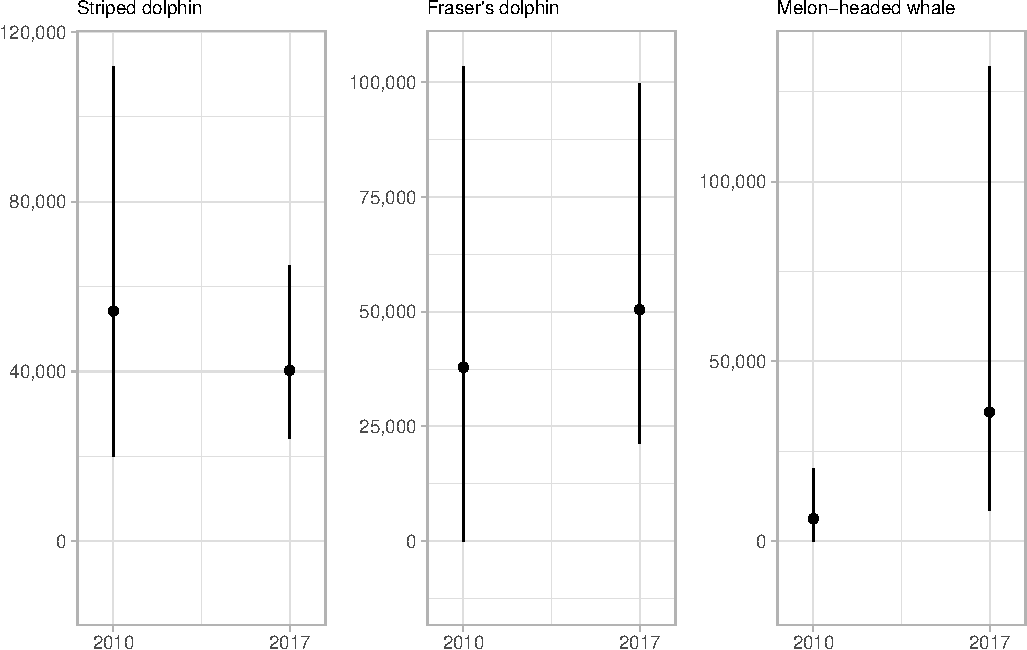
\includegraphics{figures/unnamed-chunk-320-1.pdf}

\hypertarget{detection-function-plots}{%
\section*{Detection function plots}\label{detection-function-plots}}
\addcontentsline{toc}{section}{Detection function plots}

To plot the best-fit detection model for a species pool, use the \texttt{df\_plot()} function.

\begin{Shaded}
\begin{Highlighting}[]
\FunctionTok{df\_plot}\NormalTok{(lta\_result)}
\end{Highlighting}
\end{Shaded}

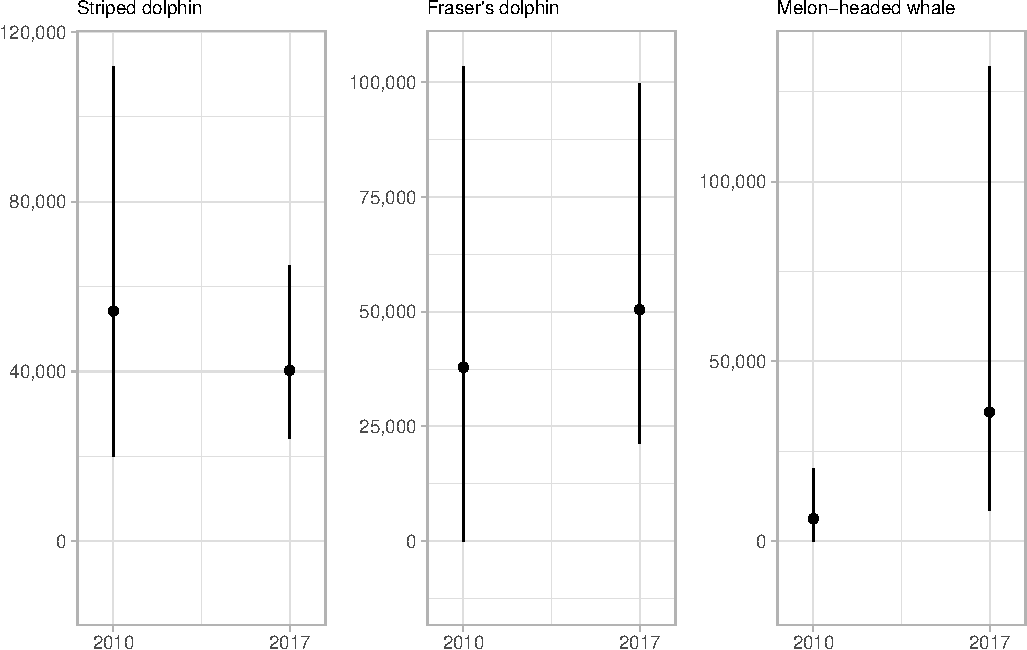
\includegraphics{figures/unnamed-chunk-321-1.pdf}

This function provides various stylization options, including the option to show multiple best-fitting models atop a single histogram of detections:

\begin{Shaded}
\begin{Highlighting}[]
\FunctionTok{df\_plot}\NormalTok{(lta\_result,}
        \AttributeTok{model\_colors=}\NormalTok{RColorBrewer}\SpecialCharTok{::}\FunctionTok{brewer.pal}\NormalTok{(}\AttributeTok{n =} \DecValTok{4}\NormalTok{, }\AttributeTok{name =} \StringTok{"Dark2"}\NormalTok{),}
        \AttributeTok{model\_pch =} \DecValTok{16}\NormalTok{,}
        \AttributeTok{pt\_show=}\DecValTok{2}\NormalTok{,}
        \AttributeTok{pt\_alpha=}\NormalTok{.}\DecValTok{3}\NormalTok{,}
        \AttributeTok{bootstrap\_show =} \ConstantTok{FALSE}\NormalTok{,}
        \AttributeTok{legend\_show=}\ConstantTok{TRUE}\NormalTok{,}
        \AttributeTok{legend\_x=}\FloatTok{2.8}\NormalTok{)}
\end{Highlighting}
\end{Shaded}

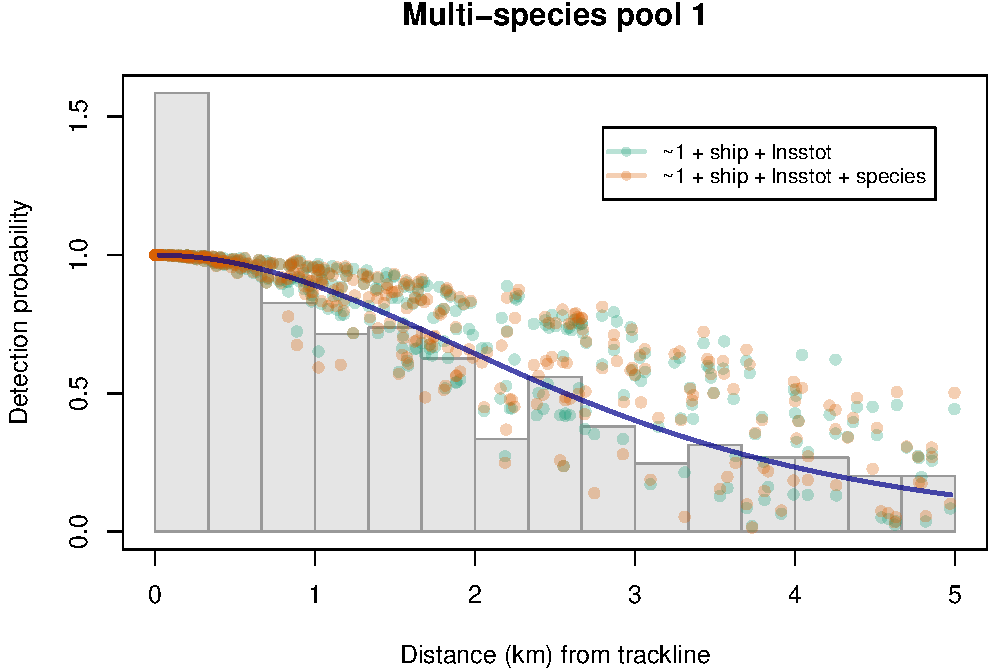
\includegraphics{figures/unnamed-chunk-322-1.pdf}

\hypertarget{part-case-studies}{%
\part{Case studies}\label{part-case-studies}}

\hypertarget{whiceas}{%
\chapter{WHICEAS}\label{whiceas}}

Here we demonstrate code that reproduces the Bradford et al.~(2022) WHICEAS report within the new \texttt{LTabundR} framework. This study estimates cetacean abundance for Hawaiian WHICEAS study area for 2017 and 2020. Here we use survey data from 1986 to 2020 to estimate \emph{Relative g(0)} and detection functions. Currently, coefficients of variation (CV) of density and abundance are estimated using only 100 bootstrap iterations (the publication uses 1,000) to reduce processing time.

\begin{Shaded}
\begin{Highlighting}[]
\FunctionTok{library}\NormalTok{(dplyr)}
\FunctionTok{library}\NormalTok{(LTabundR)}
\FunctionTok{library}\NormalTok{(ggplot2)}
\end{Highlighting}
\end{Shaded}

\hypertarget{data-processing}{%
\section*{Data processing}\label{data-processing}}
\addcontentsline{toc}{section}{Data processing}

\hypertarget{settings-1}{%
\subsection*{Settings}\label{settings-1}}
\addcontentsline{toc}{subsection}{Settings}

\hypertarget{survey-wide-settings-2}{%
\subsubsection*{Survey-wide settings}\label{survey-wide-settings-2}}
\addcontentsline{toc}{subsubsection}{Survey-wide settings}

\begin{Shaded}
\begin{Highlighting}[]
\FunctionTok{data}\NormalTok{(species\_codes)}
\FunctionTok{data}\NormalTok{(ships)}
\FunctionTok{data}\NormalTok{(group\_size\_coefficients)}
\NormalTok{edits }\OtherTok{\textless{}{-}} \FunctionTok{readRDS}\NormalTok{(}\StringTok{\textquotesingle{}cnp\_1986\_2020\_edits.RData\textquotesingle{}}\NormalTok{)}

\NormalTok{survey }\OtherTok{\textless{}{-}} \FunctionTok{load\_survey\_settings}\NormalTok{(}
  \AttributeTok{out\_handling =} \StringTok{\textquotesingle{}remove\textquotesingle{}}\NormalTok{,}
  \AttributeTok{max\_row\_interval =} \ConstantTok{Inf}\NormalTok{,}
  \AttributeTok{segment\_method =} \StringTok{"equallength"}\NormalTok{,}
  \AttributeTok{segment\_target\_km =} \DecValTok{150}\NormalTok{,}
  \AttributeTok{segment\_max\_interval =} \DecValTok{24}\NormalTok{,}
  \AttributeTok{segment\_remainder\_handling =} \FunctionTok{c}\NormalTok{(}\StringTok{"segment"}\NormalTok{),}
  \AttributeTok{ship\_list =}\NormalTok{ ships,}
  \AttributeTok{species\_codes =}\NormalTok{ species\_codes,}
  \AttributeTok{group\_size\_coefficients =}\NormalTok{ group\_size\_coefficients,}
  \AttributeTok{smear\_angles =} \ConstantTok{FALSE}
\NormalTok{)}
\end{Highlighting}
\end{Shaded}

\hypertarget{geostrata-1}{%
\subsubsection*{Geostrata}\label{geostrata-1}}
\addcontentsline{toc}{subsubsection}{Geostrata}

\begin{Shaded}
\begin{Highlighting}[]
\FunctionTok{data}\NormalTok{(strata\_cnp)}
\end{Highlighting}
\end{Shaded}

\hypertarget{cohort-specific-settings-1}{%
\subsubsection*{Cohort-specific settings}\label{cohort-specific-settings-1}}
\addcontentsline{toc}{subsubsection}{Cohort-specific settings}

\hypertarget{cohort-1-all-species}{%
\paragraph*{Cohort 1: all species}\label{cohort-1-all-species}}
\addcontentsline{toc}{paragraph}{Cohort 1: all species}

\begin{Shaded}
\begin{Highlighting}[]
\NormalTok{all\_species }\OtherTok{\textless{}{-}} \FunctionTok{load\_cohort\_settings}\NormalTok{(}
  \AttributeTok{id =} \StringTok{"all"}\NormalTok{, }\CommentTok{\# *}
  \AttributeTok{species =} \ConstantTok{NULL}\NormalTok{, }
  \AttributeTok{strata =} \FunctionTok{c}\NormalTok{(}\StringTok{\textquotesingle{}WHICEAS\textquotesingle{}}\NormalTok{, }\StringTok{\textquotesingle{}HI\_EEZ\textquotesingle{}}\NormalTok{, }\StringTok{\textquotesingle{}OtherCNP\textquotesingle{}}\NormalTok{), }\CommentTok{\# *}
  \AttributeTok{probable\_species =} \ConstantTok{FALSE}\NormalTok{,}
  \AttributeTok{sighting\_method =} \DecValTok{0}\NormalTok{,}
  \AttributeTok{cue\_range =} \DecValTok{0}\SpecialCharTok{:}\DecValTok{7}\NormalTok{,}
  \AttributeTok{school\_size\_range =} \FunctionTok{c}\NormalTok{(}\DecValTok{0}\NormalTok{, }\DecValTok{10000}\NormalTok{),}
  \AttributeTok{school\_size\_calibrate =} \ConstantTok{TRUE}\NormalTok{,}
  \AttributeTok{calibration\_floor =} \DecValTok{0}\NormalTok{,}
  \AttributeTok{use\_low\_if\_na =} \ConstantTok{TRUE}\NormalTok{,}
  \AttributeTok{io\_sightings =} \DecValTok{0}\NormalTok{,}
  \AttributeTok{geometric\_mean\_group =} \ConstantTok{TRUE}\NormalTok{,}
  \AttributeTok{truncation\_km =} \FloatTok{7.5}\NormalTok{, }\CommentTok{\# *}
  \AttributeTok{beaufort\_range =} \DecValTok{0}\SpecialCharTok{:}\DecValTok{6}\NormalTok{,}
  \AttributeTok{abeam\_sightings =} \ConstantTok{TRUE}\NormalTok{,}
  \AttributeTok{strata\_overlap\_handling =} \FunctionTok{c}\NormalTok{(}\StringTok{"smallest"}\NormalTok{),}
  \AttributeTok{distance\_types =} \FunctionTok{c}\NormalTok{(}\StringTok{\textquotesingle{}S\textquotesingle{}}\NormalTok{,}\StringTok{\textquotesingle{}F\textquotesingle{}}\NormalTok{,}\StringTok{\textquotesingle{}N\textquotesingle{}}\NormalTok{),}
  \AttributeTok{distance\_modes =} \FunctionTok{c}\NormalTok{(}\StringTok{\textquotesingle{}P\textquotesingle{}}\NormalTok{,}\StringTok{\textquotesingle{}C\textquotesingle{}}\NormalTok{),}
  \AttributeTok{distance\_on\_off =} \ConstantTok{TRUE}
\NormalTok{)}
\end{Highlighting}
\end{Shaded}

\hypertarget{cohort-2-bottlenose-dolphins}{%
\paragraph*{Cohort 2: bottlenose dolphins}\label{cohort-2-bottlenose-dolphins}}
\addcontentsline{toc}{paragraph}{Cohort 2: bottlenose dolphins}

\begin{Shaded}
\begin{Highlighting}[]
\NormalTok{bottlenose }\OtherTok{\textless{}{-}} \FunctionTok{load\_cohort\_settings}\NormalTok{(}
  \AttributeTok{id =} \StringTok{"bottlenose"}\NormalTok{,}
  \AttributeTok{species =} \FunctionTok{c}\NormalTok{(}\StringTok{\textquotesingle{}015\textquotesingle{}}\NormalTok{, }\StringTok{\textquotesingle{}018\textquotesingle{}}\NormalTok{, }\StringTok{\textquotesingle{}021\textquotesingle{}}\NormalTok{, }\StringTok{\textquotesingle{}032\textquotesingle{}}\NormalTok{),}
  \AttributeTok{strata =} \FunctionTok{c}\NormalTok{(}\StringTok{\textquotesingle{}WHICEAS\textquotesingle{}}\NormalTok{, }\StringTok{\textquotesingle{}HI\_EEZ\textquotesingle{}}\NormalTok{, }\StringTok{\textquotesingle{}OtherCNP\textquotesingle{}}\NormalTok{,}
             \StringTok{\textquotesingle{}Bottlenose\_BI\textquotesingle{}}\NormalTok{, }\StringTok{\textquotesingle{}Bottlenose\_OUFI\textquotesingle{}}\NormalTok{, }\StringTok{\textquotesingle{}Bottlenose\_KaNi\textquotesingle{}}\NormalTok{),}
  \AttributeTok{truncation\_km =} \FloatTok{7.5}\NormalTok{)}
\end{Highlighting}
\end{Shaded}

\hypertarget{cohort-3-pantropical-spotted-dolphins}{%
\paragraph*{Cohort 3: pantropical spotted dolphins}\label{cohort-3-pantropical-spotted-dolphins}}
\addcontentsline{toc}{paragraph}{Cohort 3: pantropical spotted dolphins}

\begin{Shaded}
\begin{Highlighting}[]
\NormalTok{spotted }\OtherTok{\textless{}{-}} \FunctionTok{load\_cohort\_settings}\NormalTok{(}
  \AttributeTok{id =} \StringTok{"spotted"}\NormalTok{,}
  \AttributeTok{species =} \StringTok{\textquotesingle{}002\textquotesingle{}}\NormalTok{,}
  \AttributeTok{strata =} \FunctionTok{c}\NormalTok{(}\StringTok{\textquotesingle{}WHICEAS\textquotesingle{}}\NormalTok{, }\StringTok{\textquotesingle{}HI\_EEZ\textquotesingle{}}\NormalTok{, }\StringTok{\textquotesingle{}OtherCNP\textquotesingle{}}\NormalTok{,}
             \StringTok{\textquotesingle{}Spotted\_OU\textquotesingle{}}\NormalTok{,}\StringTok{\textquotesingle{}Spotted\_FI\textquotesingle{}}\NormalTok{,}\StringTok{\textquotesingle{}Spotted\_BI\textquotesingle{}}\NormalTok{),}
  \AttributeTok{truncation\_km =} \FloatTok{7.5}\NormalTok{)}
\end{Highlighting}
\end{Shaded}

\hypertarget{process}{%
\subsection*{Process}\label{process}}
\addcontentsline{toc}{subsection}{Process}

\begin{Shaded}
\begin{Highlighting}[]
\NormalTok{settings }\OtherTok{\textless{}{-}} \FunctionTok{load\_settings}\NormalTok{(}\AttributeTok{strata =}\NormalTok{ strata\_cnp,}
                          \AttributeTok{survey =}\NormalTok{ survey,}
                          \AttributeTok{cohorts =} \FunctionTok{list}\NormalTok{(all\_species,}
\NormalTok{                                         bottlenose,}
\NormalTok{                                         spotted))}

\NormalTok{cruz }\OtherTok{\textless{}{-}} 
  \FunctionTok{process\_surveys}\NormalTok{(}\AttributeTok{das\_file =} \StringTok{\textquotesingle{}data/surveys/CenPac1986{-}2020\_Final\_alb.das\textquotesingle{}}\NormalTok{,}
                  \AttributeTok{settings =}\NormalTok{ settings,}
                  \AttributeTok{edits =}\NormalTok{ edits) }

\FunctionTok{save}\NormalTok{(cruz, }\AttributeTok{file=}\StringTok{\textquotesingle{}whiceas/whiceas\_cruz.RData\textquotesingle{}}\NormalTok{)}
\end{Highlighting}
\end{Shaded}

\begin{Shaded}
\begin{Highlighting}[]
\FunctionTok{load}\NormalTok{(}\StringTok{\textquotesingle{}whiceas/whiceas\_cruz.RData\textquotesingle{}}\NormalTok{)}
\end{Highlighting}
\end{Shaded}

\hypertarget{data-exploration}{%
\section*{Data exploration}\label{data-exploration}}
\addcontentsline{toc}{section}{Data exploration}

\hypertarget{processed-data-structure}{%
\subsection*{Processed data structure}\label{processed-data-structure}}
\addcontentsline{toc}{subsection}{Processed data structure}

\begin{Shaded}
\begin{Highlighting}[]
\FunctionTok{cruz\_structure}\NormalTok{(cruz)}
\end{Highlighting}
\end{Shaded}

\hypertarget{map-of-sightings}{%
\subsection*{Map of sightings}\label{map-of-sightings}}
\addcontentsline{toc}{subsection}{Map of sightings}

For the entire \texttt{cruz} object:

\begin{Shaded}
\begin{Highlighting}[]
\FunctionTok{map\_cruz}\NormalTok{(cruz, }\AttributeTok{sightings\_color =} \StringTok{\textquotesingle{}firebrick\textquotesingle{}}\NormalTok{)}
\end{Highlighting}
\end{Shaded}

For just the surveys of interest:

\begin{Shaded}
\begin{Highlighting}[]
\CommentTok{\# Filter}
\NormalTok{cruz1720 }\OtherTok{\textless{}{-}} \FunctionTok{filter\_cruz}\NormalTok{(cruz, }
                        \AttributeTok{years =} \FunctionTok{c}\NormalTok{(}\DecValTok{2017}\NormalTok{, }\DecValTok{2020}\NormalTok{), }
                        \AttributeTok{regions =} \StringTok{\textquotesingle{}WHICEAS\textquotesingle{}}\NormalTok{,}
                        \AttributeTok{eff\_types =} \StringTok{\textquotesingle{}S\textquotesingle{}}\NormalTok{,}
                        \AttributeTok{bft\_range =} \DecValTok{0}\SpecialCharTok{:}\DecValTok{6}\NormalTok{)}

\CommentTok{\# Map, including survey tracks}
\FunctionTok{map\_cruz}\NormalTok{(cruz1720,}
         \AttributeTok{sightings\_color =} \StringTok{\textquotesingle{}firebrick\textquotesingle{}}\NormalTok{, }
         \AttributeTok{effort\_show =} \ConstantTok{TRUE}\NormalTok{, }
         \AttributeTok{effort\_resolution =} \DecValTok{3}\NormalTok{,}
         \AttributeTok{effort\_weight =} \DecValTok{4}\NormalTok{,}
         \AttributeTok{effort\_opacity =}\NormalTok{ .}\DecValTok{4}\NormalTok{)}
\end{Highlighting}
\end{Shaded}

\hypertarget{interactive-dashboard-1}{%
\subsection*{Interactive dashboard}\label{interactive-dashboard-1}}
\addcontentsline{toc}{subsection}{Interactive dashboard}

Use this to determine truncation distances. Note them in your \texttt{lta()} code below:

\begin{Shaded}
\begin{Highlighting}[]
\FunctionTok{cruz\_explorer}\NormalTok{(cruz)}
\end{Highlighting}
\end{Shaded}

\hypertarget{rg0-1}{%
\section*{Rg0}\label{rg0-1}}
\addcontentsline{toc}{section}{Rg0}

We can use the built-in dataset, \texttt{data(g0\_results)}, which has Beaufort-specific \emph{Relative g(0)} estimates for most species based on 1986-2020 surveys.

\begin{Shaded}
\begin{Highlighting}[]
\FunctionTok{data}\NormalTok{(}\StringTok{"g0\_results"}\NormalTok{)}
\NormalTok{Rg0 }\OtherTok{\textless{}{-}}\NormalTok{ g0\_results}
\end{Highlighting}
\end{Shaded}

\begin{Shaded}
\begin{Highlighting}[]
\CommentTok{\# Plot the results: }
\FunctionTok{g0\_plot}\NormalTok{(Rg0, }\AttributeTok{panes =} \DecValTok{3}\NormalTok{)}
\end{Highlighting}
\end{Shaded}

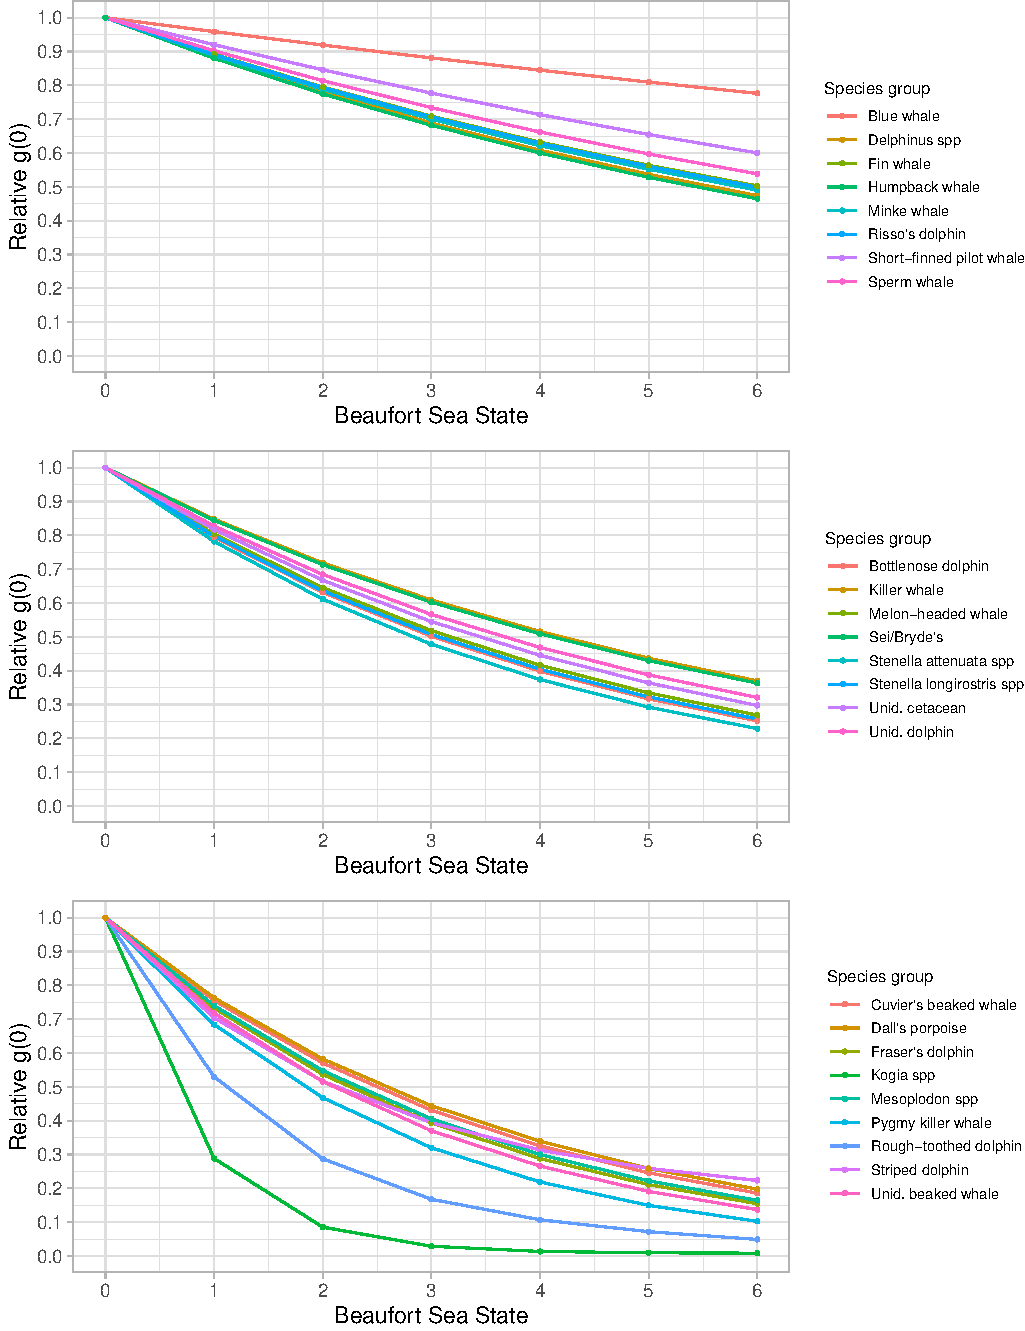
\includegraphics{figures/unnamed-chunk-338-1.pdf}

To explore the effects of \texttt{LTabundR}'s \emph{g(0)} estimation routines on our abundance estimates, we will be running the analyses below with three different \emph{g(0)} scenarios. In scenario 1, we will manually specify the weighted \texttt{g(0)} and its CV for each species in 2020; these results should be nearly exact replicates of those from Bradford et al.~(2021), and we can be sure that any discrepancy between the two sets of results are not attributable the \emph{g(0)} aspect of the analysis. Second, we will allow \texttt{LTabundR} to calculate the weighted \texttt{g(0)} and its CV using the same \emph{Relative g(0)} values that were used in Bradford et al.~(2021) (i.e., the results of Barlow (2015), which used surveys from 1986 to 2010 and is provided in \texttt{LTabundR} as a built-in dataset), such that any difference between scenarios 1 and 2 are likely due to the weighted \emph{g(0)} subroutines. Finally, in scenario 3, we will use the \emph{Relative g(0)} esitmates produced by \texttt{LTabundR} using a more extensive survey dataset (1986-2020).

For each \emph{g(0)} scenario, our \texttt{Rg0} object and \texttt{results\_path} will differ:

\begin{Shaded}
\begin{Highlighting}[]
\CommentTok{\# Specify scenario number here}
\NormalTok{g0\_scenario }\OtherTok{\textless{}{-}} \DecValTok{2}
\end{Highlighting}
\end{Shaded}

\begin{Shaded}
\begin{Highlighting}[]
\CommentTok{\# Set Rg0 source and results path}
\ControlFlowTok{if}\NormalTok{(g0\_scenario }\SpecialCharTok{==} \DecValTok{1}\NormalTok{)\{ }\CommentTok{\# Using manually{-}specified g0 and its CV}
\NormalTok{  Rg0 }\OtherTok{\textless{}{-}} \ConstantTok{NULL}
\NormalTok{  results\_path }\OtherTok{\textless{}{-}} \StringTok{\textquotesingle{}whiceas/lta\_manual/\textquotesingle{}}
\NormalTok{\}}
\ControlFlowTok{if}\NormalTok{(g0\_scenario }\SpecialCharTok{==} \DecValTok{2}\NormalTok{)\{ }\CommentTok{\# Using Rg0 estimates from Barlow 2015}
  \FunctionTok{data}\NormalTok{(barlow\_2015)}
\NormalTok{  Rg0 }\OtherTok{\textless{}{-}}\NormalTok{ barlow\_2015}
\NormalTok{  results\_path }\OtherTok{\textless{}{-}} \StringTok{\textquotesingle{}whiceas/lta\_barlow/\textquotesingle{}}
\NormalTok{\}}
\ControlFlowTok{if}\NormalTok{(g0\_scenario }\SpecialCharTok{==} \DecValTok{3}\NormalTok{)\{ }\CommentTok{\# New LTabundR estimates of Rg0}
  \FunctionTok{data}\NormalTok{(g0\_results)}
\NormalTok{  Rg0 }\OtherTok{\textless{}{-}}\NormalTok{ g0\_results}
\NormalTok{  results\_path }\OtherTok{\textless{}{-}} \StringTok{\textquotesingle{}whiceas/lta/\textquotesingle{}}
\NormalTok{\}}
\end{Highlighting}
\end{Shaded}

\hypertarget{density-abundance}{%
\section*{Density \& abundance}\label{density-abundance}}
\addcontentsline{toc}{section}{Density \& abundance}

First we can define common values that will be constant across all estimates we produce:

\begin{Shaded}
\begin{Highlighting}[]
\NormalTok{bootstraps }\OtherTok{\textless{}{-}} \DecValTok{200}
\NormalTok{years }\OtherTok{\textless{}{-}} \DecValTok{1986}\SpecialCharTok{:}\DecValTok{2020}
\NormalTok{fit\_regions }\OtherTok{\textless{}{-}} \ConstantTok{NULL}
\NormalTok{fit\_not\_regions }\OtherTok{\textless{}{-}} \ConstantTok{NULL}
\NormalTok{toplot }\OtherTok{=} \ConstantTok{TRUE}
\NormalTok{verbose }\OtherTok{=} \ConstantTok{TRUE}

\NormalTok{df\_settings }\OtherTok{\textless{}{-}}
  \FunctionTok{list}\NormalTok{(}\AttributeTok{covariates =} \FunctionTok{c}\NormalTok{(}\StringTok{\textquotesingle{}bft\textquotesingle{}}\NormalTok{,}\StringTok{\textquotesingle{}lnsstot\textquotesingle{}}\NormalTok{,}\StringTok{\textquotesingle{}cruise\textquotesingle{}}\NormalTok{,}\StringTok{\textquotesingle{}year\textquotesingle{}}\NormalTok{,}\StringTok{\textquotesingle{}ship\textquotesingle{}}\NormalTok{,}\StringTok{\textquotesingle{}species\textquotesingle{}}\NormalTok{),}
       \AttributeTok{covariates\_factor =} \FunctionTok{c}\NormalTok{(}\ConstantTok{FALSE}\NormalTok{, }\ConstantTok{FALSE}\NormalTok{, }\ConstantTok{TRUE}\NormalTok{, }\ConstantTok{TRUE}\NormalTok{, }\ConstantTok{TRUE}\NormalTok{, }\ConstantTok{TRUE}\NormalTok{),}
       \AttributeTok{covariates\_levels =} \DecValTok{2}\NormalTok{,}
       \AttributeTok{covariates\_n\_per\_level =} \DecValTok{10}\NormalTok{,}
       \AttributeTok{simplify\_cue =} \ConstantTok{TRUE}\NormalTok{,}
       \AttributeTok{simplify\_bino =} \ConstantTok{TRUE}\NormalTok{,}
       \AttributeTok{detection\_function\_base =} \StringTok{\textquotesingle{}hn\textquotesingle{}}\NormalTok{,}
       \AttributeTok{base\_model =} \StringTok{\textquotesingle{}\textasciitilde{}1\textquotesingle{}}\NormalTok{,}
       \AttributeTok{delta\_aic =} \DecValTok{2}\NormalTok{)}
\end{Highlighting}
\end{Shaded}

For most species, we want to estimate density/abundance for the same set of year-region scenarios. To reduce code redundancy, as well as the risk of typing errors (and our work!), we can use the \texttt{LTabundR} function \texttt{lta\_estimates()} to economize how we prepare our \texttt{estimates} input.

For most species, these are the year-region scenarios for which we want estimates:

\begin{Shaded}
\begin{Highlighting}[]
\NormalTok{scenarios }\OtherTok{\textless{}{-}} \FunctionTok{list}\NormalTok{(}\FunctionTok{list}\NormalTok{(}\AttributeTok{years =} \DecValTok{2017}\NormalTok{,}
                       \AttributeTok{regions =} \StringTok{\textquotesingle{}WHICEAS\textquotesingle{}}\NormalTok{),}
                  \FunctionTok{list}\NormalTok{(}\AttributeTok{years =} \DecValTok{2020}\NormalTok{, }
                       \AttributeTok{regions =} \StringTok{\textquotesingle{}WHICEAS\textquotesingle{}}\NormalTok{))}
\end{Highlighting}
\end{Shaded}

The \texttt{lta\_estimates()} function will generate a custom function that makes it easy to create a set of \texttt{estimates} sub-lists for each species of interest:

\begin{Shaded}
\begin{Highlighting}[]
\NormalTok{estimator }\OtherTok{\textless{}{-}} \FunctionTok{lta\_estimates}\NormalTok{(scenarios)}
\end{Highlighting}
\end{Shaded}

That result, \texttt{estimator}, is actually a function. Here's an example of how this function will work, using the first species pool as an example:

\begin{Shaded}
\begin{Highlighting}[]
\NormalTok{estimates }\OtherTok{\textless{}{-}}
  \FunctionTok{c}\NormalTok{(}\FunctionTok{estimator}\NormalTok{(}\AttributeTok{spp =} \StringTok{\textquotesingle{}013\textquotesingle{}}\NormalTok{, }\AttributeTok{title =} \StringTok{"Striped dolphin"}\NormalTok{),}
    \FunctionTok{estimator}\NormalTok{(}\AttributeTok{spp =} \StringTok{\textquotesingle{}026\textquotesingle{}}\NormalTok{, }\AttributeTok{title =} \StringTok{"Fraser\textquotesingle{}s dolphin"}\NormalTok{, }\AttributeTok{alt\_g0\_spp =} \StringTok{\textquotesingle{}013\textquotesingle{}}\NormalTok{),}
    \FunctionTok{estimator}\NormalTok{(}\AttributeTok{spp =} \StringTok{\textquotesingle{}031\textquotesingle{}}\NormalTok{, }\AttributeTok{title =} \StringTok{"Melon{-}headed whale"}\NormalTok{, }\AttributeTok{alt\_g0\_spp =} \StringTok{\textquotesingle{}013\textquotesingle{}}\NormalTok{))}

\NormalTok{estimates  }
\NormalTok{[[}\DecValTok{1}\NormalTok{]]}
\NormalTok{[[}\DecValTok{1}\NormalTok{]]}\SpecialCharTok{$}\NormalTok{years}
\NormalTok{[}\DecValTok{1}\NormalTok{] }\DecValTok{2017}

\NormalTok{[[}\DecValTok{1}\NormalTok{]]}\SpecialCharTok{$}\NormalTok{regions}
\NormalTok{[}\DecValTok{1}\NormalTok{] }\StringTok{"WHICEAS"}

\NormalTok{[[}\DecValTok{1}\NormalTok{]]}\SpecialCharTok{$}\NormalTok{spp}
\NormalTok{[}\DecValTok{1}\NormalTok{] }\StringTok{"013"}

\NormalTok{[[}\DecValTok{1}\NormalTok{]]}\SpecialCharTok{$}\NormalTok{title}
\NormalTok{[}\DecValTok{1}\NormalTok{] }\StringTok{"Striped dolphin"}


\NormalTok{[[}\DecValTok{2}\NormalTok{]]}
\NormalTok{[[}\DecValTok{2}\NormalTok{]]}\SpecialCharTok{$}\NormalTok{years}
\NormalTok{[}\DecValTok{1}\NormalTok{] }\DecValTok{2020}

\NormalTok{[[}\DecValTok{2}\NormalTok{]]}\SpecialCharTok{$}\NormalTok{regions}
\NormalTok{[}\DecValTok{1}\NormalTok{] }\StringTok{"WHICEAS"}

\NormalTok{[[}\DecValTok{2}\NormalTok{]]}\SpecialCharTok{$}\NormalTok{spp}
\NormalTok{[}\DecValTok{1}\NormalTok{] }\StringTok{"013"}

\NormalTok{[[}\DecValTok{2}\NormalTok{]]}\SpecialCharTok{$}\NormalTok{title}
\NormalTok{[}\DecValTok{1}\NormalTok{] }\StringTok{"Striped dolphin"}


\NormalTok{[[}\DecValTok{3}\NormalTok{]]}
\NormalTok{[[}\DecValTok{3}\NormalTok{]]}\SpecialCharTok{$}\NormalTok{years}
\NormalTok{[}\DecValTok{1}\NormalTok{] }\DecValTok{2017}

\NormalTok{[[}\DecValTok{3}\NormalTok{]]}\SpecialCharTok{$}\NormalTok{regions}
\NormalTok{[}\DecValTok{1}\NormalTok{] }\StringTok{"WHICEAS"}

\NormalTok{[[}\DecValTok{3}\NormalTok{]]}\SpecialCharTok{$}\NormalTok{spp}
\NormalTok{[}\DecValTok{1}\NormalTok{] }\StringTok{"026"}

\NormalTok{[[}\DecValTok{3}\NormalTok{]]}\SpecialCharTok{$}\NormalTok{title}
\NormalTok{[}\DecValTok{1}\NormalTok{] }\StringTok{"Fraser\textquotesingle{}s dolphin"}

\NormalTok{[[}\DecValTok{3}\NormalTok{]]}\SpecialCharTok{$}\NormalTok{alt\_g0\_spp}
\NormalTok{[}\DecValTok{1}\NormalTok{] }\StringTok{"013"}


\NormalTok{[[}\DecValTok{4}\NormalTok{]]}
\NormalTok{[[}\DecValTok{4}\NormalTok{]]}\SpecialCharTok{$}\NormalTok{years}
\NormalTok{[}\DecValTok{1}\NormalTok{] }\DecValTok{2020}

\NormalTok{[[}\DecValTok{4}\NormalTok{]]}\SpecialCharTok{$}\NormalTok{regions}
\NormalTok{[}\DecValTok{1}\NormalTok{] }\StringTok{"WHICEAS"}

\NormalTok{[[}\DecValTok{4}\NormalTok{]]}\SpecialCharTok{$}\NormalTok{spp}
\NormalTok{[}\DecValTok{1}\NormalTok{] }\StringTok{"026"}

\NormalTok{[[}\DecValTok{4}\NormalTok{]]}\SpecialCharTok{$}\NormalTok{title}
\NormalTok{[}\DecValTok{1}\NormalTok{] }\StringTok{"Fraser\textquotesingle{}s dolphin"}

\NormalTok{[[}\DecValTok{4}\NormalTok{]]}\SpecialCharTok{$}\NormalTok{alt\_g0\_spp}
\NormalTok{[}\DecValTok{1}\NormalTok{] }\StringTok{"013"}


\NormalTok{[[}\DecValTok{5}\NormalTok{]]}
\NormalTok{[[}\DecValTok{5}\NormalTok{]]}\SpecialCharTok{$}\NormalTok{years}
\NormalTok{[}\DecValTok{1}\NormalTok{] }\DecValTok{2017}

\NormalTok{[[}\DecValTok{5}\NormalTok{]]}\SpecialCharTok{$}\NormalTok{regions}
\NormalTok{[}\DecValTok{1}\NormalTok{] }\StringTok{"WHICEAS"}

\NormalTok{[[}\DecValTok{5}\NormalTok{]]}\SpecialCharTok{$}\NormalTok{spp}
\NormalTok{[}\DecValTok{1}\NormalTok{] }\StringTok{"031"}

\NormalTok{[[}\DecValTok{5}\NormalTok{]]}\SpecialCharTok{$}\NormalTok{title}
\NormalTok{[}\DecValTok{1}\NormalTok{] }\StringTok{"Melon{-}headed whale"}

\NormalTok{[[}\DecValTok{5}\NormalTok{]]}\SpecialCharTok{$}\NormalTok{alt\_g0\_spp}
\NormalTok{[}\DecValTok{1}\NormalTok{] }\StringTok{"013"}


\NormalTok{[[}\DecValTok{6}\NormalTok{]]}
\NormalTok{[[}\DecValTok{6}\NormalTok{]]}\SpecialCharTok{$}\NormalTok{years}
\NormalTok{[}\DecValTok{1}\NormalTok{] }\DecValTok{2020}

\NormalTok{[[}\DecValTok{6}\NormalTok{]]}\SpecialCharTok{$}\NormalTok{regions}
\NormalTok{[}\DecValTok{1}\NormalTok{] }\StringTok{"WHICEAS"}

\NormalTok{[[}\DecValTok{6}\NormalTok{]]}\SpecialCharTok{$}\NormalTok{spp}
\NormalTok{[}\DecValTok{1}\NormalTok{] }\StringTok{"031"}

\NormalTok{[[}\DecValTok{6}\NormalTok{]]}\SpecialCharTok{$}\NormalTok{title}
\NormalTok{[}\DecValTok{1}\NormalTok{] }\StringTok{"Melon{-}headed whale"}

\NormalTok{[[}\DecValTok{6}\NormalTok{]]}\SpecialCharTok{$}\NormalTok{alt\_g0\_spp}
\NormalTok{[}\DecValTok{1}\NormalTok{] }\StringTok{"013"}
\end{Highlighting}
\end{Shaded}

The output of \texttt{estimator()} is a list of sub-lists specifying a set of density/abundance estimates you want to produce based on the detection function for a single species pool.

Here is the full code for producing those estimates for all species from Bradford et al.~(2021):

\hypertarget{multi-species-pool-1}{%
\subsection*{Multi-species pool 1}\label{multi-species-pool-1}}
\addcontentsline{toc}{subsection}{Multi-species pool 1}

\begin{Shaded}
\begin{Highlighting}[]
\CommentTok{\# Striped dolphin (013), Fraser\textquotesingle{}s dolphin (026), Melon{-}headed whale (031)}

\ControlFlowTok{if}\NormalTok{(}\ConstantTok{TRUE}\NormalTok{)\{ }\CommentTok{\# toggle}

  \CommentTok{\# Detection function specifications}
\NormalTok{  fit\_filters }\OtherTok{\textless{}{-}}
    \FunctionTok{list}\NormalTok{(}\AttributeTok{spp =} \FunctionTok{c}\NormalTok{(}\StringTok{\textquotesingle{}013\textquotesingle{}}\NormalTok{, }\StringTok{\textquotesingle{}026\textquotesingle{}}\NormalTok{, }\StringTok{\textquotesingle{}031\textquotesingle{}}\NormalTok{),}
         \AttributeTok{pool =} \StringTok{\textquotesingle{}Multi{-}species pool 1\textquotesingle{}}\NormalTok{,}
         \AttributeTok{cohort =} \StringTok{\textquotesingle{}all\textquotesingle{}}\NormalTok{,}
         \AttributeTok{truncation\_distance =} \DecValTok{5}\NormalTok{,}
         \AttributeTok{other\_species =} \StringTok{\textquotesingle{}remove\textquotesingle{}}\NormalTok{,}
         \AttributeTok{years =}\NormalTok{ years,}
         \AttributeTok{regions =}\NormalTok{ fit\_regions,}
         \AttributeTok{not\_regions =}\NormalTok{ fit\_not\_regions)}

  \CommentTok{\# Density / abundance estimation plan}
\NormalTok{  estimates }\OtherTok{\textless{}{-}}
    \FunctionTok{c}\NormalTok{(}\FunctionTok{estimator}\NormalTok{(}\AttributeTok{spp =} \StringTok{\textquotesingle{}013\textquotesingle{}}\NormalTok{, }\AttributeTok{title =} \StringTok{"Striped dolphin"}\NormalTok{),}
      \FunctionTok{estimator}\NormalTok{(}\AttributeTok{spp =} \StringTok{\textquotesingle{}026\textquotesingle{}}\NormalTok{, }\AttributeTok{title =} \StringTok{"Fraser\textquotesingle{}s dolphin"}\NormalTok{, }\AttributeTok{alt\_g0\_spp =} \StringTok{\textquotesingle{}013\textquotesingle{}}\NormalTok{),}
      \FunctionTok{estimator}\NormalTok{(}\AttributeTok{spp =} \StringTok{\textquotesingle{}031\textquotesingle{}}\NormalTok{, }\AttributeTok{title =} \StringTok{"Melon{-}headed whale"}\NormalTok{, }\AttributeTok{alt\_g0\_spp =} \StringTok{\textquotesingle{}013\textquotesingle{}}\NormalTok{))}
  
\NormalTok{  estimates}
  
  \CommentTok{\# Manually specify g0 and its CV {-}{-} only for g0\_scenario 1}
  \CommentTok{\# Two specifications per species, one for 2017 and one for 2020}
  \ControlFlowTok{if}\NormalTok{(g0\_scenario}\SpecialCharTok{==}\DecValTok{1}\NormalTok{)\{}
    \CommentTok{\# Striped }
\NormalTok{    estimates[[}\DecValTok{1}\NormalTok{]]}\SpecialCharTok{$}\NormalTok{g0 }\OtherTok{\textless{}{-}} \FloatTok{0.35}\NormalTok{; estimates[[}\DecValTok{1}\NormalTok{]]}\SpecialCharTok{$}\NormalTok{g0\_cv }\OtherTok{\textless{}{-}} \FloatTok{0.19}
\NormalTok{    estimates[[}\DecValTok{2}\NormalTok{]]}\SpecialCharTok{$}\NormalTok{g0 }\OtherTok{\textless{}{-}} \FloatTok{0.31}\NormalTok{; estimates[[}\DecValTok{2}\NormalTok{]]}\SpecialCharTok{$}\NormalTok{g0\_cv }\OtherTok{\textless{}{-}} \FloatTok{0.22}
    \CommentTok{\# Fraser\textquotesingle{}s}
\NormalTok{    estimates[[}\DecValTok{3}\NormalTok{]]}\SpecialCharTok{$}\NormalTok{g0 }\OtherTok{\textless{}{-}} \FloatTok{0.35}\NormalTok{; estimates[[}\DecValTok{3}\NormalTok{]]}\SpecialCharTok{$}\NormalTok{g0\_cv }\OtherTok{\textless{}{-}} \FloatTok{0.10}
\NormalTok{    estimates[[}\DecValTok{4}\NormalTok{]]}\SpecialCharTok{$}\NormalTok{g0 }\OtherTok{\textless{}{-}} \FloatTok{0.31}\NormalTok{; estimates[[}\DecValTok{4}\NormalTok{]]}\SpecialCharTok{$}\NormalTok{g0\_cv }\OtherTok{\textless{}{-}} \FloatTok{0.22}
    \CommentTok{\# Melon{-}headed}
\NormalTok{    estimates[[}\DecValTok{5}\NormalTok{]]}\SpecialCharTok{$}\NormalTok{g0 }\OtherTok{\textless{}{-}} \FloatTok{0.35}\NormalTok{; estimates[[}\DecValTok{5}\NormalTok{]]}\SpecialCharTok{$}\NormalTok{g0\_cv }\OtherTok{\textless{}{-}} \FloatTok{0.19}
\NormalTok{    estimates[[}\DecValTok{6}\NormalTok{]]}\SpecialCharTok{$}\NormalTok{g0 }\OtherTok{\textless{}{-}} \FloatTok{0.31}\NormalTok{; estimates[[}\DecValTok{6}\NormalTok{]]}\SpecialCharTok{$}\NormalTok{g0\_cv }\OtherTok{\textless{}{-}} \FloatTok{0.22}
\NormalTok{  \}}
  
  \CommentTok{\# Run analysis}
\NormalTok{  results }\OtherTok{\textless{}{-}} \FunctionTok{lta}\NormalTok{(cruz, Rg0, fit\_filters, df\_settings, estimates,}
                 \AttributeTok{bootstraps =}\NormalTok{ bootstraps,}
                 \AttributeTok{toplot=}\NormalTok{toplot, }\AttributeTok{verbose=}\NormalTok{verbose)}

  \CommentTok{\# Save result}
\NormalTok{  (results\_file }\OtherTok{\textless{}{-}} \FunctionTok{paste0}\NormalTok{(results\_path, fit\_filters}\SpecialCharTok{$}\NormalTok{pool, }\StringTok{\textquotesingle{}.RData\textquotesingle{}}\NormalTok{))}
  \FunctionTok{saveRDS}\NormalTok{(results, }\AttributeTok{file=}\NormalTok{results\_file)}
\NormalTok{\}}
\end{Highlighting}
\end{Shaded}

\hypertarget{multi-species-pool-2}{%
\subsection*{Multi-species pool 2}\label{multi-species-pool-2}}
\addcontentsline{toc}{subsection}{Multi-species pool 2}

\begin{Shaded}
\begin{Highlighting}[]
\CommentTok{\# Rough{-}toothed dolphin (15), Common bottlenose dolphin (18), Risso\textquotesingle{}s (21),}
\CommentTok{\# Pygmy killer whale (32)}

\CommentTok{\# Notes}
\CommentTok{\# Bottlenose abundance is estimated in a separate cohort, but included here for DF fitting}

\ControlFlowTok{if}\NormalTok{(}\ConstantTok{TRUE}\NormalTok{)\{ }\CommentTok{\# toggle}

  \CommentTok{\# Detection function specifications}
\NormalTok{  fit\_filters }\OtherTok{\textless{}{-}}
    \FunctionTok{list}\NormalTok{(}\AttributeTok{spp =} \FunctionTok{c}\NormalTok{(}\StringTok{\textquotesingle{}015\textquotesingle{}}\NormalTok{, }\StringTok{\textquotesingle{}018\textquotesingle{}}\NormalTok{, }\StringTok{\textquotesingle{}021\textquotesingle{}}\NormalTok{, }\StringTok{\textquotesingle{}032\textquotesingle{}}\NormalTok{),}
         \AttributeTok{pool =} \StringTok{\textquotesingle{}Multi{-}species pool 2\textquotesingle{}}\NormalTok{,}
         \AttributeTok{cohort =} \StringTok{\textquotesingle{}all\textquotesingle{}}\NormalTok{,}
         \AttributeTok{truncation\_distance =} \DecValTok{5}\NormalTok{,}
         \AttributeTok{years =}\NormalTok{ years,}
         \AttributeTok{regions =}\NormalTok{ fit\_regions,}
         \AttributeTok{not\_regions =}\NormalTok{ fit\_not\_regions)}

  \CommentTok{\# Density / abundance estimation plan}
\NormalTok{  estimates }\OtherTok{\textless{}{-}}
      \FunctionTok{c}\NormalTok{(}\FunctionTok{estimator}\NormalTok{(}\AttributeTok{spp =} \StringTok{\textquotesingle{}015\textquotesingle{}}\NormalTok{, }\AttributeTok{title =} \StringTok{"Rough{-}toothed dolphin"}\NormalTok{),}
        \FunctionTok{estimator}\NormalTok{(}\AttributeTok{spp =} \StringTok{\textquotesingle{}021\textquotesingle{}}\NormalTok{, }\AttributeTok{title =} \StringTok{"Risso\textquotesingle{}s dolphin"}\NormalTok{),}
        \FunctionTok{estimator}\NormalTok{(}\AttributeTok{spp =} \StringTok{\textquotesingle{}032\textquotesingle{}}\NormalTok{, }\AttributeTok{title =} \StringTok{"Pygmy killer whale"}\NormalTok{))}

  \ControlFlowTok{if}\NormalTok{(g0\_scenario}\SpecialCharTok{==}\DecValTok{1}\NormalTok{)\{}
    \CommentTok{\# Rough{-}toothed }
\NormalTok{    estimates[[}\DecValTok{1}\NormalTok{]]}\SpecialCharTok{$}\NormalTok{g0 }\OtherTok{\textless{}{-}} \FloatTok{0.09}\NormalTok{; estimates[[}\DecValTok{1}\NormalTok{]]}\SpecialCharTok{$}\NormalTok{g0\_cv }\OtherTok{\textless{}{-}} \FloatTok{0.45}
\NormalTok{    estimates[[}\DecValTok{2}\NormalTok{]]}\SpecialCharTok{$}\NormalTok{g0 }\OtherTok{\textless{}{-}} \FloatTok{0.07}\NormalTok{; estimates[[}\DecValTok{2}\NormalTok{]]}\SpecialCharTok{$}\NormalTok{g0\_cv }\OtherTok{\textless{}{-}} \FloatTok{0.51}
    \CommentTok{\# Risso\textquotesingle{}s}
\NormalTok{    estimates[[}\DecValTok{3}\NormalTok{]]}\SpecialCharTok{$}\NormalTok{g0 }\OtherTok{\textless{}{-}} \FloatTok{0.57}\NormalTok{; estimates[[}\DecValTok{3}\NormalTok{]]}\SpecialCharTok{$}\NormalTok{g0\_cv }\OtherTok{\textless{}{-}} \FloatTok{0.18}
\NormalTok{    estimates[[}\DecValTok{4}\NormalTok{]]}\SpecialCharTok{$}\NormalTok{g0 }\OtherTok{\textless{}{-}} \FloatTok{0.52}\NormalTok{; estimates[[}\DecValTok{4}\NormalTok{]]}\SpecialCharTok{$}\NormalTok{g0\_cv }\OtherTok{\textless{}{-}} \DecValTok{021}
    \CommentTok{\# Pygmy killer}
\NormalTok{    estimates[[}\DecValTok{5}\NormalTok{]]}\SpecialCharTok{$}\NormalTok{g0 }\OtherTok{\textless{}{-}} \FloatTok{0.14}\NormalTok{; estimates[[}\DecValTok{5}\NormalTok{]]}\SpecialCharTok{$}\NormalTok{g0\_cv }\OtherTok{\textless{}{-}} \FloatTok{0.25}
\NormalTok{    estimates[[}\DecValTok{6}\NormalTok{]]}\SpecialCharTok{$}\NormalTok{g0 }\OtherTok{\textless{}{-}} \FloatTok{0.11}\NormalTok{; estimates[[}\DecValTok{6}\NormalTok{]]}\SpecialCharTok{$}\NormalTok{g0\_cv }\OtherTok{\textless{}{-}} \FloatTok{0.28}
\NormalTok{  \}}
  
  \CommentTok{\# Run analysis}
\NormalTok{  results }\OtherTok{\textless{}{-}} \FunctionTok{lta}\NormalTok{(cruz, Rg0, fit\_filters, df\_settings, estimates,}
                 \AttributeTok{use\_g0 =} \ConstantTok{TRUE}\NormalTok{,}
                 \AttributeTok{bootstraps =}\NormalTok{ bootstraps,}
                 \AttributeTok{toplot=}\NormalTok{toplot, }\AttributeTok{verbose=}\NormalTok{verbose)}

  \CommentTok{\# Save result}
\NormalTok{  (results\_file }\OtherTok{\textless{}{-}} \FunctionTok{paste0}\NormalTok{(results\_path, fit\_filters}\SpecialCharTok{$}\NormalTok{pool, }\StringTok{\textquotesingle{}.RData\textquotesingle{}}\NormalTok{))}
  \FunctionTok{saveRDS}\NormalTok{(results, }\AttributeTok{file=}\NormalTok{results\_file)}
\NormalTok{\}}
\end{Highlighting}
\end{Shaded}

\hypertarget{multi-species-pool-3}{%
\subsection*{Multi-species pool 3}\label{multi-species-pool-3}}
\addcontentsline{toc}{subsection}{Multi-species pool 3}

\begin{Shaded}
\begin{Highlighting}[]
\CommentTok{\# Short{-}finned pilot whale (036), Longman\textquotesingle{}s beaked whale (065)}

\CommentTok{\# No Rg(0) available for Longman\textquotesingle{}s {-}{-} will use SF pilot whale instead to estimate its weighted g0}

\ControlFlowTok{if}\NormalTok{(}\ConstantTok{TRUE}\NormalTok{)\{ }\CommentTok{\# toggle}

  \CommentTok{\# Detection function specifications}
\NormalTok{  fit\_filters }\OtherTok{\textless{}{-}}
    \FunctionTok{list}\NormalTok{(}\AttributeTok{spp =} \FunctionTok{c}\NormalTok{(}\StringTok{\textquotesingle{}036\textquotesingle{}}\NormalTok{, }\StringTok{\textquotesingle{}065\textquotesingle{}}\NormalTok{),}
         \AttributeTok{pool =} \StringTok{\textquotesingle{}Multi{-}species pool 3\textquotesingle{}}\NormalTok{,}
         \AttributeTok{cohort =} \StringTok{\textquotesingle{}all\textquotesingle{}}\NormalTok{,}
         \AttributeTok{truncation\_distance =} \DecValTok{5}\NormalTok{,}
         \AttributeTok{years =}\NormalTok{ years,}
         \AttributeTok{regions =}\NormalTok{ fit\_regions,}
         \AttributeTok{not\_regions =}\NormalTok{ fit\_not\_regions)}

  \CommentTok{\# Density / abundance estimation plan}
\NormalTok{  estimates }\OtherTok{\textless{}{-}}
    \FunctionTok{c}\NormalTok{(}\FunctionTok{estimator}\NormalTok{(}\AttributeTok{spp =} \StringTok{\textquotesingle{}036\textquotesingle{}}\NormalTok{, }\AttributeTok{title =} \StringTok{"Short{-}finned pilot whale"}\NormalTok{),}
      \FunctionTok{estimator}\NormalTok{(}\AttributeTok{spp =} \StringTok{\textquotesingle{}065\textquotesingle{}}\NormalTok{, }\AttributeTok{title =} \StringTok{"Longman\textquotesingle{}s beaked whale"}\NormalTok{, }
                \AttributeTok{alt\_g0\_spp =} \StringTok{\textquotesingle{}036\textquotesingle{}}\NormalTok{))}

  \ControlFlowTok{if}\NormalTok{(g0\_scenario}\SpecialCharTok{==}\DecValTok{1}\NormalTok{)\{}
    \CommentTok{\# Short{-}finned }
\NormalTok{    estimates[[}\DecValTok{1}\NormalTok{]]}\SpecialCharTok{$}\NormalTok{g0 }\OtherTok{\textless{}{-}} \FloatTok{0.58}\NormalTok{; estimates[[}\DecValTok{1}\NormalTok{]]}\SpecialCharTok{$}\NormalTok{g0\_cv }\OtherTok{\textless{}{-}} \FloatTok{0.15}
\NormalTok{    estimates[[}\DecValTok{2}\NormalTok{]]}\SpecialCharTok{$}\NormalTok{g0 }\OtherTok{\textless{}{-}} \FloatTok{0.52}\NormalTok{; estimates[[}\DecValTok{2}\NormalTok{]]}\SpecialCharTok{$}\NormalTok{g0\_cv }\OtherTok{\textless{}{-}} \FloatTok{0.19}
    \CommentTok{\# Longman\textquotesingle{}s}
\NormalTok{    estimates[[}\DecValTok{3}\NormalTok{]]}\SpecialCharTok{$}\NormalTok{g0 }\OtherTok{\textless{}{-}} \FloatTok{0.58}\NormalTok{; estimates[[}\DecValTok{3}\NormalTok{]]}\SpecialCharTok{$}\NormalTok{g0\_cv }\OtherTok{\textless{}{-}} \FloatTok{0.15}
\NormalTok{    estimates[[}\DecValTok{4}\NormalTok{]]}\SpecialCharTok{$}\NormalTok{g0 }\OtherTok{\textless{}{-}} \FloatTok{0.52}\NormalTok{; estimates[[}\DecValTok{4}\NormalTok{]]}\SpecialCharTok{$}\NormalTok{g0\_cv }\OtherTok{\textless{}{-}} \FloatTok{0.19}
\NormalTok{  \}}
  
  \CommentTok{\# Run analysis}
\NormalTok{  results }\OtherTok{\textless{}{-}} \FunctionTok{lta}\NormalTok{(cruz, Rg0, fit\_filters, df\_settings, estimates,}
                 \AttributeTok{use\_g0 =} \ConstantTok{TRUE}\NormalTok{,}
                 \AttributeTok{bootstraps =}\NormalTok{ bootstraps,}
                 \AttributeTok{toplot=}\NormalTok{toplot, }\AttributeTok{verbose=}\NormalTok{verbose)}

  \CommentTok{\# Save result}
\NormalTok{  (results\_file }\OtherTok{\textless{}{-}} \FunctionTok{paste0}\NormalTok{(results\_path, fit\_filters}\SpecialCharTok{$}\NormalTok{pool, }\StringTok{\textquotesingle{}.RData\textquotesingle{}}\NormalTok{))}
  \FunctionTok{saveRDS}\NormalTok{(results, }\AttributeTok{file=}\NormalTok{results\_file)}
\NormalTok{\}}
\end{Highlighting}
\end{Shaded}

\hypertarget{multi-species-pool-4}{%
\subsection*{Multi-species pool 4}\label{multi-species-pool-4}}
\addcontentsline{toc}{subsection}{Multi-species pool 4}

\begin{Shaded}
\begin{Highlighting}[]
\CommentTok{\# Killer whale (37), sperm whale (46)}

\ControlFlowTok{if}\NormalTok{(}\ConstantTok{TRUE}\NormalTok{)\{ }\CommentTok{\# toggle}

  \CommentTok{\# Detection function specifications}
\NormalTok{  fit\_filters }\OtherTok{\textless{}{-}}
    \FunctionTok{list}\NormalTok{(}\AttributeTok{spp =} \FunctionTok{c}\NormalTok{(}\StringTok{\textquotesingle{}037\textquotesingle{}}\NormalTok{, }\StringTok{\textquotesingle{}046\textquotesingle{}}\NormalTok{),}
         \AttributeTok{pool =} \StringTok{\textquotesingle{}Multi{-}species pool 4\textquotesingle{}}\NormalTok{,}
         \AttributeTok{cohort =} \StringTok{\textquotesingle{}all\textquotesingle{}}\NormalTok{,}
         \AttributeTok{truncation\_distance =} \FloatTok{5.5}\NormalTok{,}
         \AttributeTok{other\_species =} \StringTok{\textquotesingle{}remove\textquotesingle{}}\NormalTok{,}
         \AttributeTok{years =}\NormalTok{ years,}
         \AttributeTok{regions =}\NormalTok{ fit\_regions,}
         \AttributeTok{not\_regions =}\NormalTok{ fit\_not\_regions)}

  \CommentTok{\# Density / abundance estimation plan}
\NormalTok{  estimates }\OtherTok{\textless{}{-}}
      \FunctionTok{c}\NormalTok{(}\FunctionTok{estimator}\NormalTok{(}\AttributeTok{spp =} \StringTok{\textquotesingle{}037\textquotesingle{}}\NormalTok{, }\AttributeTok{title =} \StringTok{"Killer whale"}\NormalTok{),}
        \FunctionTok{estimator}\NormalTok{(}\AttributeTok{spp =} \StringTok{\textquotesingle{}046\textquotesingle{}}\NormalTok{, }\AttributeTok{title =} \StringTok{"Sperm whale"}\NormalTok{))}

  \ControlFlowTok{if}\NormalTok{(g0\_scenario}\SpecialCharTok{==}\DecValTok{1}\NormalTok{)\{}
    \CommentTok{\# Killer (no sightings in ALB et al 2021)}
\NormalTok{    estimates[[}\DecValTok{1}\NormalTok{]]}\SpecialCharTok{$}\NormalTok{g0 }\OtherTok{\textless{}{-}} \DecValTok{1}\NormalTok{; estimates[[}\DecValTok{1}\NormalTok{]]}\SpecialCharTok{$}\NormalTok{g0\_cv }\OtherTok{\textless{}{-}} \DecValTok{0}
\NormalTok{    estimates[[}\DecValTok{2}\NormalTok{]]}\SpecialCharTok{$}\NormalTok{g0 }\OtherTok{\textless{}{-}} \DecValTok{1}\NormalTok{; estimates[[}\DecValTok{2}\NormalTok{]]}\SpecialCharTok{$}\NormalTok{g0\_cv }\OtherTok{\textless{}{-}} \DecValTok{0}
    \CommentTok{\# Sperm}
\NormalTok{    estimates[[}\DecValTok{3}\NormalTok{]]}\SpecialCharTok{$}\NormalTok{g0 }\OtherTok{\textless{}{-}} \FloatTok{0.63}\NormalTok{; estimates[[}\DecValTok{3}\NormalTok{]]}\SpecialCharTok{$}\NormalTok{g0\_cv }\OtherTok{\textless{}{-}} \FloatTok{0.34}
\NormalTok{    estimates[[}\DecValTok{4}\NormalTok{]]}\SpecialCharTok{$}\NormalTok{g0 }\OtherTok{\textless{}{-}} \FloatTok{0.61}\NormalTok{; estimates[[}\DecValTok{4}\NormalTok{]]}\SpecialCharTok{$}\NormalTok{g0\_cv }\OtherTok{\textless{}{-}} \FloatTok{0.37}
\NormalTok{  \}}
  
  \CommentTok{\# Run analysis}
\NormalTok{  results }\OtherTok{\textless{}{-}} \FunctionTok{lta}\NormalTok{(cruz, Rg0, fit\_filters, df\_settings, estimates,}
                 \AttributeTok{use\_g0 =} \ConstantTok{TRUE}\NormalTok{,}
                 \AttributeTok{bootstraps =}\NormalTok{ bootstraps,}
                 \AttributeTok{toplot=}\NormalTok{toplot, }\AttributeTok{verbose=}\NormalTok{verbose)}

  \CommentTok{\# Save result}
\NormalTok{  (results\_file }\OtherTok{\textless{}{-}} \FunctionTok{paste0}\NormalTok{(results\_path, fit\_filters}\SpecialCharTok{$}\NormalTok{pool, }\StringTok{\textquotesingle{}.RData\textquotesingle{}}\NormalTok{))}
  \FunctionTok{saveRDS}\NormalTok{(results, }\AttributeTok{file=}\NormalTok{results\_file)}
\NormalTok{\}}
\end{Highlighting}
\end{Shaded}

\hypertarget{multi-species-pool-5}{%
\subsection*{Multi-species pool 5}\label{multi-species-pool-5}}
\addcontentsline{toc}{subsection}{Multi-species pool 5}

\begin{Shaded}
\begin{Highlighting}[]
\CommentTok{\# Pygmy sperm whale (47), dwarf sperm whale (48), UNID Kogia (80),}
\CommentTok{\# Blainville\textquotesingle{}s beaked whale (59), Cuvier\textquotesingle{}s beaked whale (61),}
\CommentTok{\# UNID Mesoplodon (51), UNID beaked whale (49), Minke whale (71)}

\ControlFlowTok{if}\NormalTok{(}\ConstantTok{TRUE}\NormalTok{)\{ }\CommentTok{\# toggle}

  \CommentTok{\# Detection function specifications}
\NormalTok{  fit\_filters }\OtherTok{\textless{}{-}}
    \FunctionTok{list}\NormalTok{(}\AttributeTok{spp =} \FunctionTok{c}\NormalTok{(}\StringTok{\textquotesingle{}047\textquotesingle{}}\NormalTok{, }\StringTok{\textquotesingle{}048\textquotesingle{}}\NormalTok{, }\StringTok{\textquotesingle{}080\textquotesingle{}}\NormalTok{, }\StringTok{\textquotesingle{}059\textquotesingle{}}\NormalTok{, }\StringTok{\textquotesingle{}061\textquotesingle{}}\NormalTok{, }\StringTok{\textquotesingle{}051\textquotesingle{}}\NormalTok{, }\StringTok{\textquotesingle{}049\textquotesingle{}}\NormalTok{, }\StringTok{\textquotesingle{}071\textquotesingle{}}\NormalTok{),}
         \AttributeTok{pool =} \StringTok{\textquotesingle{}Multi{-}species pool 5\textquotesingle{}}\NormalTok{,}
         \AttributeTok{cohort =} \StringTok{\textquotesingle{}all\textquotesingle{}}\NormalTok{,}
         \AttributeTok{truncation\_distance =} \FloatTok{4.5}\NormalTok{,}
         \AttributeTok{years =}\NormalTok{ years,}
         \AttributeTok{regions =}\NormalTok{ fit\_regions,}
         \AttributeTok{not\_regions =}\NormalTok{ fit\_not\_regions)}

  \CommentTok{\# Density / abundance estimation plan}
\NormalTok{  estimates }\OtherTok{\textless{}{-}}
      \FunctionTok{c}\NormalTok{(}\FunctionTok{estimator}\NormalTok{(}\AttributeTok{spp =} \StringTok{\textquotesingle{}047\textquotesingle{}}\NormalTok{, }\AttributeTok{title =} \StringTok{"Pygmy sperm whale"}\NormalTok{),}
        \FunctionTok{estimator}\NormalTok{(}\AttributeTok{spp =} \StringTok{\textquotesingle{}048\textquotesingle{}}\NormalTok{, }\AttributeTok{title =} \StringTok{"Dwarf sperm whale"}\NormalTok{),}
        \FunctionTok{estimator}\NormalTok{(}\AttributeTok{spp =} \StringTok{\textquotesingle{}080\textquotesingle{}}\NormalTok{, }\AttributeTok{title =} \StringTok{"Unidentified Kogia"}\NormalTok{),}
        \FunctionTok{estimator}\NormalTok{(}\AttributeTok{spp =} \StringTok{\textquotesingle{}059\textquotesingle{}}\NormalTok{, }\AttributeTok{title =} \StringTok{"Blainville\textquotesingle{}s beaked whale"}\NormalTok{),}
        \FunctionTok{estimator}\NormalTok{(}\AttributeTok{spp =} \StringTok{\textquotesingle{}061\textquotesingle{}}\NormalTok{, }\AttributeTok{title =} \StringTok{"Cuvier\textquotesingle{}s beaked whale"}\NormalTok{),}
        \FunctionTok{estimator}\NormalTok{(}\AttributeTok{spp =} \StringTok{\textquotesingle{}051\textquotesingle{}}\NormalTok{, }\AttributeTok{title =} \StringTok{"Unidentified Mesoplodon"}\NormalTok{),}
        \FunctionTok{estimator}\NormalTok{(}\AttributeTok{spp =} \StringTok{\textquotesingle{}049\textquotesingle{}}\NormalTok{, }
                  \AttributeTok{title =} \StringTok{"Unidentified beaked whale"}\NormalTok{,}
                  \AttributeTok{alt\_g0\_spp =} \FunctionTok{c}\NormalTok{(}\StringTok{\textquotesingle{}061\textquotesingle{}}\NormalTok{,}\StringTok{\textquotesingle{}051\textquotesingle{}}\NormalTok{),}
                  \AttributeTok{combine\_g0 =} \ConstantTok{TRUE}\NormalTok{),}
        \FunctionTok{estimator}\NormalTok{(}\AttributeTok{spp =} \StringTok{\textquotesingle{}071\textquotesingle{}}\NormalTok{, }\AttributeTok{title =} \StringTok{"Minke whale"}\NormalTok{))}

  \CommentTok{\# Note Barlow2015 provides absolute estimates for Cuviers and UNID Mesop}
  
  \ControlFlowTok{if}\NormalTok{(g0\_scenario}\SpecialCharTok{==}\DecValTok{1}\NormalTok{)\{}
    \CommentTok{\# Pygmy sperm (no sightings in ALB, using other kogia values)}
\NormalTok{    estimates[[}\DecValTok{1}\NormalTok{]]}\SpecialCharTok{$}\NormalTok{g0 }\OtherTok{\textless{}{-}} \FloatTok{0.005}\NormalTok{; estimates[[}\DecValTok{1}\NormalTok{]]}\SpecialCharTok{$}\NormalTok{g0\_cv }\OtherTok{\textless{}{-}} \FloatTok{0.15}
\NormalTok{    estimates[[}\DecValTok{2}\NormalTok{]]}\SpecialCharTok{$}\NormalTok{g0 }\OtherTok{\textless{}{-}} \FloatTok{0.004}\NormalTok{; estimates[[}\DecValTok{2}\NormalTok{]]}\SpecialCharTok{$}\NormalTok{g0\_cv }\OtherTok{\textless{}{-}} \FloatTok{0.15}
    \CommentTok{\# Dwarf sperm (no ALB sightings in 2017, using 2020 g0)}
\NormalTok{    estimates[[}\DecValTok{3}\NormalTok{]]}\SpecialCharTok{$}\NormalTok{g0 }\OtherTok{\textless{}{-}} \FloatTok{0.005}\NormalTok{; estimates[[}\DecValTok{3}\NormalTok{]]}\SpecialCharTok{$}\NormalTok{g0\_cv }\OtherTok{\textless{}{-}} \FloatTok{0.15}
\NormalTok{    estimates[[}\DecValTok{4}\NormalTok{]]}\SpecialCharTok{$}\NormalTok{g0 }\OtherTok{\textless{}{-}} \FloatTok{0.004}\NormalTok{; estimates[[}\DecValTok{4}\NormalTok{]]}\SpecialCharTok{$}\NormalTok{g0\_cv }\OtherTok{\textless{}{-}} \FloatTok{0.15}
    \CommentTok{\# UNID Kogia (no ALB sightings 2020, using 2017 g0)}
\NormalTok{    estimates[[}\DecValTok{5}\NormalTok{]]}\SpecialCharTok{$}\NormalTok{g0 }\OtherTok{\textless{}{-}} \FloatTok{0.005}\NormalTok{; estimates[[}\DecValTok{5}\NormalTok{]]}\SpecialCharTok{$}\NormalTok{g0\_cv }\OtherTok{\textless{}{-}} \FloatTok{0.15}
\NormalTok{    estimates[[}\DecValTok{6}\NormalTok{]]}\SpecialCharTok{$}\NormalTok{g0 }\OtherTok{\textless{}{-}} \FloatTok{0.004}\NormalTok{; estimates[[}\DecValTok{6}\NormalTok{]]}\SpecialCharTok{$}\NormalTok{g0\_cv }\OtherTok{\textless{}{-}} \FloatTok{0.15}
    \CommentTok{\# Blainville\textquotesingle{}s (no ALB sightings 2017, using 2020 g0)}
\NormalTok{    estimates[[}\DecValTok{7}\NormalTok{]]}\SpecialCharTok{$}\NormalTok{g0 }\OtherTok{\textless{}{-}} \FloatTok{0.11}\NormalTok{; estimates[[}\DecValTok{7}\NormalTok{]]}\SpecialCharTok{$}\NormalTok{g0\_cv }\OtherTok{\textless{}{-}} \FloatTok{0.30}
\NormalTok{    estimates[[}\DecValTok{8}\NormalTok{]]}\SpecialCharTok{$}\NormalTok{g0 }\OtherTok{\textless{}{-}} \FloatTok{0.11}\NormalTok{; estimates[[}\DecValTok{6}\NormalTok{]]}\SpecialCharTok{$}\NormalTok{g0\_cv }\OtherTok{\textless{}{-}} \FloatTok{0.30}
    \CommentTok{\# Cuvier\textquotesingle{}s (no sightings in ALB {-}{-} using unid beaked g0)}
\NormalTok{    estimates[[}\DecValTok{9}\NormalTok{]]}\SpecialCharTok{$}\NormalTok{g0 }\OtherTok{\textless{}{-}} \FloatTok{0.13}\NormalTok{; estimates[[}\DecValTok{9}\NormalTok{]]}\SpecialCharTok{$}\NormalTok{g0\_cv }\OtherTok{\textless{}{-}} \FloatTok{0.20}
\NormalTok{    estimates[[}\DecValTok{10}\NormalTok{]]}\SpecialCharTok{$}\NormalTok{g0 }\OtherTok{\textless{}{-}} \FloatTok{0.11}\NormalTok{; estimates[[}\DecValTok{10}\NormalTok{]]}\SpecialCharTok{$}\NormalTok{g0\_cv }\OtherTok{\textless{}{-}} \FloatTok{0.21}
    \CommentTok{\# UNID Mesop (no ALB sightings 2017, using 2020 g0)}
\NormalTok{    estimates[[}\DecValTok{11}\NormalTok{]]}\SpecialCharTok{$}\NormalTok{g0 }\OtherTok{\textless{}{-}} \FloatTok{0.11}\NormalTok{; estimates[[}\DecValTok{11}\NormalTok{]]}\SpecialCharTok{$}\NormalTok{g0\_cv }\OtherTok{\textless{}{-}} \FloatTok{0.30}
\NormalTok{    estimates[[}\DecValTok{12}\NormalTok{]]}\SpecialCharTok{$}\NormalTok{g0 }\OtherTok{\textless{}{-}} \FloatTok{0.11}\NormalTok{; estimates[[}\DecValTok{12}\NormalTok{]]}\SpecialCharTok{$}\NormalTok{g0\_cv }\OtherTok{\textless{}{-}} \FloatTok{0.30}
    \CommentTok{\# UNID beaked}
\NormalTok{    estimates[[}\DecValTok{13}\NormalTok{]]}\SpecialCharTok{$}\NormalTok{g0 }\OtherTok{\textless{}{-}} \FloatTok{0.13}\NormalTok{; estimates[[}\DecValTok{13}\NormalTok{]]}\SpecialCharTok{$}\NormalTok{g0\_cv }\OtherTok{\textless{}{-}} \FloatTok{0.20}
\NormalTok{    estimates[[}\DecValTok{14}\NormalTok{]]}\SpecialCharTok{$}\NormalTok{g0 }\OtherTok{\textless{}{-}} \FloatTok{0.11}\NormalTok{; estimates[[}\DecValTok{14}\NormalTok{]]}\SpecialCharTok{$}\NormalTok{g0\_cv }\OtherTok{\textless{}{-}} \FloatTok{0.21}
\NormalTok{  \}}
  
  \CommentTok{\# Run analysis}
\NormalTok{  results }\OtherTok{\textless{}{-}} \FunctionTok{lta}\NormalTok{(cruz, Rg0, fit\_filters, df\_settings, estimates,}
                 \AttributeTok{use\_g0 =} \ConstantTok{TRUE}\NormalTok{,}
                 \AttributeTok{bootstraps =}\NormalTok{ bootstraps,}
                 \AttributeTok{toplot=}\NormalTok{toplot, }\AttributeTok{verbose=}\NormalTok{verbose)}

  \CommentTok{\# Save result}
\NormalTok{  (results\_file }\OtherTok{\textless{}{-}} \FunctionTok{paste0}\NormalTok{(results\_path, fit\_filters}\SpecialCharTok{$}\NormalTok{pool, }\StringTok{\textquotesingle{}.RData\textquotesingle{}}\NormalTok{))}
  \FunctionTok{saveRDS}\NormalTok{(results, }\AttributeTok{file=}\NormalTok{results\_file)}
\NormalTok{\}}
\end{Highlighting}
\end{Shaded}

\hypertarget{multi-species-pool-6}{%
\subsection*{Multi-species pool 6}\label{multi-species-pool-6}}
\addcontentsline{toc}{subsection}{Multi-species pool 6}

\begin{Shaded}
\begin{Highlighting}[]
\CommentTok{\# Bryde\textquotesingle{}s whale (72), Sei whale (73), Fin whale (74), Blue whale (75),}
\CommentTok{\# Sei/Bryde\textquotesingle{}s (99), Fin/Sei/Bryde\textquotesingle{}s (72, 73, 74, 99)}

\CommentTok{\# Bryde\textquotesingle{}s, Sei\textquotesingle{}s, and Sei/Bryde\textquotesingle{}s all use same Rg0 (title = "Sei/Bryde\textquotesingle{}s")}
\CommentTok{\# Sei/Bryde\textquotesingle{}s/Fin use an average of Fin and Sei/Bryde\textquotesingle{}s.}

\ControlFlowTok{if}\NormalTok{(}\ConstantTok{TRUE}\NormalTok{)\{ }\CommentTok{\# toggle}

  \CommentTok{\# Detection function specifications}
\NormalTok{  fit\_filters }\OtherTok{\textless{}{-}}
    \FunctionTok{list}\NormalTok{(}\AttributeTok{spp =} \FunctionTok{c}\NormalTok{(}\StringTok{\textquotesingle{}072\textquotesingle{}}\NormalTok{, }\StringTok{\textquotesingle{}073\textquotesingle{}}\NormalTok{, }\StringTok{\textquotesingle{}074\textquotesingle{}}\NormalTok{,}\StringTok{\textquotesingle{}075\textquotesingle{}}\NormalTok{,}\StringTok{\textquotesingle{}099\textquotesingle{}}\NormalTok{),}
         \AttributeTok{pool =} \StringTok{\textquotesingle{}Multi{-}species pool 6\textquotesingle{}}\NormalTok{,}
         \AttributeTok{cohort =} \StringTok{\textquotesingle{}all\textquotesingle{}}\NormalTok{,}
         \AttributeTok{truncation\_distance =} \FloatTok{5.0}\NormalTok{,}
         \AttributeTok{years =}\NormalTok{ years,}
         \AttributeTok{regions =}\NormalTok{ fit\_regions,}
         \AttributeTok{not\_regions =}\NormalTok{ fit\_not\_regions)}

  \CommentTok{\# Density / abundance estimation plan}
\NormalTok{   estimates }\OtherTok{\textless{}{-}}
      \FunctionTok{c}\NormalTok{(}\FunctionTok{estimator}\NormalTok{(}\AttributeTok{spp =} \StringTok{\textquotesingle{}072\textquotesingle{}}\NormalTok{, }\AttributeTok{title =} \StringTok{"Bryde\textquotesingle{}s whale"}\NormalTok{),}
        \FunctionTok{estimator}\NormalTok{(}\AttributeTok{spp =} \StringTok{\textquotesingle{}073\textquotesingle{}}\NormalTok{, }\AttributeTok{title =} \StringTok{"Sei whale"}\NormalTok{),}
        \FunctionTok{estimator}\NormalTok{(}\AttributeTok{spp =} \StringTok{\textquotesingle{}074\textquotesingle{}}\NormalTok{, }\AttributeTok{title =} \StringTok{"Fin whale"}\NormalTok{),}
        \FunctionTok{estimator}\NormalTok{(}\AttributeTok{spp =} \StringTok{\textquotesingle{}075\textquotesingle{}}\NormalTok{, }\AttributeTok{title =} \StringTok{"Blue whale"}\NormalTok{),}
        \FunctionTok{estimator}\NormalTok{(}\AttributeTok{spp =} \StringTok{\textquotesingle{}099\textquotesingle{}}\NormalTok{, }\AttributeTok{title =} \StringTok{"Sei/Bryde\textquotesingle{}s whale"}\NormalTok{),}
        \FunctionTok{estimator}\NormalTok{(}\AttributeTok{spp =} \FunctionTok{c}\NormalTok{(}\StringTok{\textquotesingle{}072\textquotesingle{}}\NormalTok{, }\StringTok{\textquotesingle{}073\textquotesingle{}}\NormalTok{, }\StringTok{\textquotesingle{}099\textquotesingle{}}\NormalTok{, }\StringTok{\textquotesingle{}074\textquotesingle{}}\NormalTok{), }
                  \AttributeTok{title =} \StringTok{"Sei/Bryde\textquotesingle{}s/Fin whale"}\NormalTok{,}
                  \AttributeTok{combine\_g0 =} \ConstantTok{TRUE}\NormalTok{))}
  
   \ControlFlowTok{if}\NormalTok{(g0\_scenario}\SpecialCharTok{==}\DecValTok{1}\NormalTok{)\{}
    \CommentTok{\# Brydes (no ALB sightings {-}{-} using sei values)}
\NormalTok{    estimates[[}\DecValTok{1}\NormalTok{]]}\SpecialCharTok{$}\NormalTok{g0 }\OtherTok{\textless{}{-}} \FloatTok{0.38}\NormalTok{; estimates[[}\DecValTok{1}\NormalTok{]]}\SpecialCharTok{$}\NormalTok{g0\_cv }\OtherTok{\textless{}{-}} \FloatTok{0.21}
\NormalTok{    estimates[[}\DecValTok{2}\NormalTok{]]}\SpecialCharTok{$}\NormalTok{g0 }\OtherTok{\textless{}{-}} \FloatTok{0.38}\NormalTok{; estimates[[}\DecValTok{2}\NormalTok{]]}\SpecialCharTok{$}\NormalTok{g0\_cv }\OtherTok{\textless{}{-}} \FloatTok{0.21}
    \CommentTok{\# Sei (no ALB sightings in 2017, using 2020 g0)}
\NormalTok{    estimates[[}\DecValTok{3}\NormalTok{]]}\SpecialCharTok{$}\NormalTok{g0 }\OtherTok{\textless{}{-}} \FloatTok{0.38}\NormalTok{; estimates[[}\DecValTok{3}\NormalTok{]]}\SpecialCharTok{$}\NormalTok{g0\_cv }\OtherTok{\textless{}{-}} \FloatTok{0.21}
\NormalTok{    estimates[[}\DecValTok{4}\NormalTok{]]}\SpecialCharTok{$}\NormalTok{g0 }\OtherTok{\textless{}{-}} \FloatTok{0.38}\NormalTok{; estimates[[}\DecValTok{4}\NormalTok{]]}\SpecialCharTok{$}\NormalTok{g0\_cv }\OtherTok{\textless{}{-}} \FloatTok{0.21}
    \CommentTok{\# Fin (no ALB sightings in 2017, using 2020 g0)}
\NormalTok{    estimates[[}\DecValTok{5}\NormalTok{]]}\SpecialCharTok{$}\NormalTok{g0 }\OtherTok{\textless{}{-}} \FloatTok{0.30}\NormalTok{; estimates[[}\DecValTok{5}\NormalTok{]]}\SpecialCharTok{$}\NormalTok{g0\_cv }\OtherTok{\textless{}{-}} \FloatTok{0.29}
\NormalTok{    estimates[[}\DecValTok{6}\NormalTok{]]}\SpecialCharTok{$}\NormalTok{g0 }\OtherTok{\textless{}{-}} \FloatTok{0.30}\NormalTok{; estimates[[}\DecValTok{6}\NormalTok{]]}\SpecialCharTok{$}\NormalTok{g0\_cv }\OtherTok{\textless{}{-}} \FloatTok{0.29}
    \CommentTok{\# Blue (no ALB sightings, using fin values)}
\NormalTok{    estimates[[}\DecValTok{7}\NormalTok{]]}\SpecialCharTok{$}\NormalTok{g0 }\OtherTok{\textless{}{-}} \FloatTok{0.30}\NormalTok{; estimates[[}\DecValTok{7}\NormalTok{]]}\SpecialCharTok{$}\NormalTok{g0\_cv }\OtherTok{\textless{}{-}} \FloatTok{0.29}
\NormalTok{    estimates[[}\DecValTok{8}\NormalTok{]]}\SpecialCharTok{$}\NormalTok{g0 }\OtherTok{\textless{}{-}} \FloatTok{0.30}\NormalTok{; estimates[[}\DecValTok{8}\NormalTok{]]}\SpecialCharTok{$}\NormalTok{g0\_cv }\OtherTok{\textless{}{-}} \FloatTok{0.29}
    \CommentTok{\# Sei / Bryde\textquotesingle{}s (no ALB sightings in 2017, using 2020 g0)}
\NormalTok{    estimates[[}\DecValTok{9}\NormalTok{]]}\SpecialCharTok{$}\NormalTok{g0 }\OtherTok{\textless{}{-}} \FloatTok{0.38}\NormalTok{; estimates[[}\DecValTok{9}\NormalTok{]]}\SpecialCharTok{$}\NormalTok{g0\_cv }\OtherTok{\textless{}{-}} \FloatTok{0.21}
\NormalTok{    estimates[[}\DecValTok{10}\NormalTok{]]}\SpecialCharTok{$}\NormalTok{g0 }\OtherTok{\textless{}{-}} \FloatTok{0.38}\NormalTok{; estimates[[}\DecValTok{10}\NormalTok{]]}\SpecialCharTok{$}\NormalTok{g0\_cv }\OtherTok{\textless{}{-}} \FloatTok{0.21}
    \CommentTok{\# Sei / Bryde\textquotesingle{}s / Fin (no ALB sightings in 2017, using 2020 g0)}
\NormalTok{    estimates[[}\DecValTok{11}\NormalTok{]]}\SpecialCharTok{$}\NormalTok{g0 }\OtherTok{\textless{}{-}} \FloatTok{0.34}\NormalTok{; estimates[[}\DecValTok{11}\NormalTok{]]}\SpecialCharTok{$}\NormalTok{g0\_cv }\OtherTok{\textless{}{-}} \FloatTok{0.17}
\NormalTok{    estimates[[}\DecValTok{12}\NormalTok{]]}\SpecialCharTok{$}\NormalTok{g0 }\OtherTok{\textless{}{-}} \FloatTok{0.34}\NormalTok{; estimates[[}\DecValTok{12}\NormalTok{]]}\SpecialCharTok{$}\NormalTok{g0\_cv }\OtherTok{\textless{}{-}} \FloatTok{0.17}
\NormalTok{  \}}
  
  \CommentTok{\# Run analysis}
\NormalTok{  results }\OtherTok{\textless{}{-}} \FunctionTok{lta}\NormalTok{(cruz, Rg0, fit\_filters, df\_settings, estimates,}
                 \AttributeTok{use\_g0 =} \ConstantTok{TRUE}\NormalTok{,}
                 \AttributeTok{bootstraps =}\NormalTok{ bootstraps,}
                 \AttributeTok{toplot=}\NormalTok{toplot, }\AttributeTok{verbose=}\NormalTok{verbose)}

  \CommentTok{\# Save result}
\NormalTok{  (results\_file }\OtherTok{\textless{}{-}} \FunctionTok{paste0}\NormalTok{(results\_path, fit\_filters}\SpecialCharTok{$}\NormalTok{pool, }\StringTok{\textquotesingle{}.RData\textquotesingle{}}\NormalTok{))}
  \FunctionTok{saveRDS}\NormalTok{(results, }\AttributeTok{file=}\NormalTok{results\_file)}
\NormalTok{\}}
\end{Highlighting}
\end{Shaded}

\hypertarget{humpback-whale}{%
\subsection*{Humpback whale}\label{humpback-whale}}
\addcontentsline{toc}{subsection}{Humpback whale}

\begin{Shaded}
\begin{Highlighting}[]
\ControlFlowTok{if}\NormalTok{(}\ConstantTok{TRUE}\NormalTok{)\{ }\CommentTok{\# toggle}

  \CommentTok{\# Detection function specifications}
\NormalTok{  fit\_filters }\OtherTok{\textless{}{-}}
    \FunctionTok{list}\NormalTok{(}\AttributeTok{spp =} \FunctionTok{c}\NormalTok{(}\StringTok{\textquotesingle{}076\textquotesingle{}}\NormalTok{),}
         \AttributeTok{pool =} \StringTok{\textquotesingle{}Humpback whale\textquotesingle{}}\NormalTok{,}
         \AttributeTok{cohort =} \StringTok{\textquotesingle{}all\textquotesingle{}}\NormalTok{,}
         \AttributeTok{truncation\_distance =} \FloatTok{5.5}\NormalTok{,}
         \AttributeTok{years =}\NormalTok{ years,}
         \AttributeTok{regions =}\NormalTok{ fit\_regions,}
         \AttributeTok{not\_regions =}\NormalTok{ fit\_not\_regions)}

  \CommentTok{\# Density / abundance estimation plan}
\NormalTok{   estimates }\OtherTok{\textless{}{-}}\FunctionTok{c}\NormalTok{(}\FunctionTok{estimator}\NormalTok{(}\AttributeTok{spp =} \StringTok{\textquotesingle{}076\textquotesingle{}}\NormalTok{, }\AttributeTok{title =} \StringTok{"Humpback whale"}\NormalTok{))}
   
   \ControlFlowTok{if}\NormalTok{(g0\_scenario}\SpecialCharTok{==}\DecValTok{1}\NormalTok{)\{}
    \CommentTok{\# No ALB sightings in 2017, using 2020 g0}
\NormalTok{    estimates[[}\DecValTok{1}\NormalTok{]]}\SpecialCharTok{$}\NormalTok{g0 }\OtherTok{\textless{}{-}} \FloatTok{0.68}\NormalTok{; estimates[[}\DecValTok{1}\NormalTok{]]}\SpecialCharTok{$}\NormalTok{g0\_cv }\OtherTok{\textless{}{-}} \FloatTok{0.36}
\NormalTok{    estimates[[}\DecValTok{2}\NormalTok{]]}\SpecialCharTok{$}\NormalTok{g0 }\OtherTok{\textless{}{-}} \FloatTok{0.68}\NormalTok{; estimates[[}\DecValTok{2}\NormalTok{]]}\SpecialCharTok{$}\NormalTok{g0\_cv }\OtherTok{\textless{}{-}} \FloatTok{0.36}
\NormalTok{   \}}
  
  \CommentTok{\# Run analysis}
\NormalTok{  results }\OtherTok{\textless{}{-}} \FunctionTok{lta}\NormalTok{(cruz, Rg0, fit\_filters, df\_settings, estimates,}
                 \AttributeTok{use\_g0 =} \ConstantTok{TRUE}\NormalTok{,}
                 \AttributeTok{bootstraps =}\NormalTok{ bootstraps,}
                 \AttributeTok{toplot=}\NormalTok{toplot, }\AttributeTok{verbose=}\NormalTok{verbose)}

  \CommentTok{\# Save result}
\NormalTok{  (results\_file }\OtherTok{\textless{}{-}} \FunctionTok{paste0}\NormalTok{(results\_path, fit\_filters}\SpecialCharTok{$}\NormalTok{pool, }\StringTok{\textquotesingle{}.RData\textquotesingle{}}\NormalTok{))}
  \FunctionTok{saveRDS}\NormalTok{(results, }\AttributeTok{file=}\NormalTok{results\_file)}
\NormalTok{\}}
\end{Highlighting}
\end{Shaded}

\hypertarget{unidentified-rorquals}{%
\subsection*{Unidentified rorquals}\label{unidentified-rorquals}}
\addcontentsline{toc}{subsection}{Unidentified rorquals}

\begin{Shaded}
\begin{Highlighting}[]
\CommentTok{\# UNID rorquals (70)}

\ControlFlowTok{if}\NormalTok{(}\ConstantTok{TRUE}\NormalTok{)\{ }\CommentTok{\# toggle}

  \CommentTok{\# Detection function specifications}
\NormalTok{  fit\_filters }\OtherTok{\textless{}{-}}
    \FunctionTok{list}\NormalTok{(}\AttributeTok{spp =} \FunctionTok{c}\NormalTok{(}\StringTok{\textquotesingle{}070\textquotesingle{}}\NormalTok{),}
         \AttributeTok{pool =} \StringTok{\textquotesingle{}Unidentified rorqual\textquotesingle{}}\NormalTok{,}
         \AttributeTok{cohort =} \StringTok{\textquotesingle{}all\textquotesingle{}}\NormalTok{,}
         \AttributeTok{truncation\_distance =} \FloatTok{5.5}\NormalTok{,}
         \AttributeTok{years =}\NormalTok{ years,}
         \AttributeTok{regions =}\NormalTok{ fit\_regions,}
         \AttributeTok{not\_regions =}\NormalTok{ fit\_not\_regions)}

  \CommentTok{\# Density / abundance estimation plan}
\NormalTok{  estimates }\OtherTok{\textless{}{-}}
      \FunctionTok{c}\NormalTok{(}\FunctionTok{estimator}\NormalTok{(}\AttributeTok{spp =} \StringTok{\textquotesingle{}070\textquotesingle{}}\NormalTok{, }
                  \AttributeTok{title =} \StringTok{"Unidentified rorqual"}\NormalTok{,}
                  \AttributeTok{alt\_g0\_spp =} \FunctionTok{c}\NormalTok{(}\StringTok{\textquotesingle{}071\textquotesingle{}}\NormalTok{,}\StringTok{\textquotesingle{}099\textquotesingle{}}\NormalTok{,}\StringTok{\textquotesingle{}074\textquotesingle{}}\NormalTok{,}\StringTok{\textquotesingle{}075\textquotesingle{}}\NormalTok{),}
                  \AttributeTok{combine\_g0 =} \ConstantTok{TRUE}\NormalTok{))}
  
  \ControlFlowTok{if}\NormalTok{(g0\_scenario}\SpecialCharTok{==}\DecValTok{1}\NormalTok{)\{}
\NormalTok{    estimates[[}\DecValTok{1}\NormalTok{]]}\SpecialCharTok{$}\NormalTok{g0 }\OtherTok{\textless{}{-}} \FloatTok{0.35}\NormalTok{; estimates[[}\DecValTok{1}\NormalTok{]]}\SpecialCharTok{$}\NormalTok{g0\_cv }\OtherTok{\textless{}{-}} \FloatTok{0.18}
\NormalTok{    estimates[[}\DecValTok{2}\NormalTok{]]}\SpecialCharTok{$}\NormalTok{g0 }\OtherTok{\textless{}{-}} \FloatTok{0.32}\NormalTok{; estimates[[}\DecValTok{2}\NormalTok{]]}\SpecialCharTok{$}\NormalTok{g0\_cv }\OtherTok{\textless{}{-}} \FloatTok{0.20}
\NormalTok{  \}}
  
  \CommentTok{\# Run analysis}
\NormalTok{  results }\OtherTok{\textless{}{-}} \FunctionTok{lta}\NormalTok{(cruz, Rg0, fit\_filters, df\_settings, estimates,}
                 \AttributeTok{use\_g0 =} \ConstantTok{TRUE}\NormalTok{,}
                 \AttributeTok{bootstraps =}\NormalTok{ bootstraps,}
                 \AttributeTok{toplot=}\NormalTok{toplot, }\AttributeTok{verbose=}\NormalTok{verbose)}

\NormalTok{  results}\SpecialCharTok{$}\NormalTok{bootstrap}\SpecialCharTok{$}\NormalTok{summary }\SpecialCharTok{\%\textgreater{}\%}\NormalTok{ as.data.frame}
  
  \CommentTok{\# Save result}
\NormalTok{  (results\_file }\OtherTok{\textless{}{-}} \FunctionTok{paste0}\NormalTok{(results\_path, fit\_filters}\SpecialCharTok{$}\NormalTok{pool, }\StringTok{\textquotesingle{}.RData\textquotesingle{}}\NormalTok{))}
  \FunctionTok{saveRDS}\NormalTok{(results, }\AttributeTok{file=}\NormalTok{results\_file)}
\NormalTok{\}}
\end{Highlighting}
\end{Shaded}

\hypertarget{unidentified-dolphins}{%
\subsection*{Unidentified dolphins}\label{unidentified-dolphins}}
\addcontentsline{toc}{subsection}{Unidentified dolphins}

\begin{Shaded}
\begin{Highlighting}[]
\CommentTok{\# UNID dolphin (177, 277, 377, 77)}

\ControlFlowTok{if}\NormalTok{(}\ConstantTok{TRUE}\NormalTok{)\{ }\CommentTok{\# toggle}

\NormalTok{  spp }\OtherTok{\textless{}{-}} \FunctionTok{c}\NormalTok{(}\StringTok{\textquotesingle{}177\textquotesingle{}}\NormalTok{,}\StringTok{\textquotesingle{}277\textquotesingle{}}\NormalTok{,}\StringTok{\textquotesingle{}377\textquotesingle{}}\NormalTok{,}\StringTok{\textquotesingle{}077\textquotesingle{}}\NormalTok{)}
\NormalTok{  pool\_title }\OtherTok{\textless{}{-}} \StringTok{\textquotesingle{}Unidentified dolphin\textquotesingle{}}

  \CommentTok{\# Detection function specifications}
\NormalTok{  fit\_filters }\OtherTok{\textless{}{-}}
    \FunctionTok{list}\NormalTok{(}\AttributeTok{spp =} \FunctionTok{c}\NormalTok{(}\StringTok{\textquotesingle{}177\textquotesingle{}}\NormalTok{,}\StringTok{\textquotesingle{}277\textquotesingle{}}\NormalTok{,}\StringTok{\textquotesingle{}377\textquotesingle{}}\NormalTok{,}\StringTok{\textquotesingle{}077\textquotesingle{}}\NormalTok{),}
         \AttributeTok{pool =}\NormalTok{ pool\_title,}
         \AttributeTok{cohort =} \StringTok{\textquotesingle{}all\textquotesingle{}}\NormalTok{,}
         \AttributeTok{truncation\_distance =} \FloatTok{5.5}\NormalTok{,}
         \AttributeTok{other\_species =} \StringTok{\textquotesingle{}coerce\textquotesingle{}}\NormalTok{,}
         \AttributeTok{years =}\NormalTok{ years,}
         \AttributeTok{regions =}\NormalTok{ fit\_regions,}
         \AttributeTok{not\_regions =}\NormalTok{ fit\_not\_regions)}

  \CommentTok{\# Density / abundance estimation plan}
\NormalTok{  estimates }\OtherTok{\textless{}{-}} \FunctionTok{estimator}\NormalTok{(}\AttributeTok{spp =}\NormalTok{ spp, }
                         \AttributeTok{title =}\NormalTok{ pool\_title,}
                         \AttributeTok{alt\_g0\_spp =} \FunctionTok{c}\NormalTok{(}\StringTok{\textquotesingle{}002\textquotesingle{}}\NormalTok{,}\StringTok{\textquotesingle{}013\textquotesingle{}}\NormalTok{,}\StringTok{\textquotesingle{}018\textquotesingle{}}\NormalTok{,}\StringTok{\textquotesingle{}015\textquotesingle{}}\NormalTok{, }\StringTok{\textquotesingle{}036\textquotesingle{}}\NormalTok{, }\StringTok{\textquotesingle{}021\textquotesingle{}}\NormalTok{),}
                         \AttributeTok{combine\_g0 =} \ConstantTok{TRUE}\NormalTok{)}
  
  \ControlFlowTok{if}\NormalTok{(g0\_scenario}\SpecialCharTok{==}\DecValTok{1}\NormalTok{)\{}
\NormalTok{    estimates[[}\DecValTok{1}\NormalTok{]]}\SpecialCharTok{$}\NormalTok{g0 }\OtherTok{\textless{}{-}} \FloatTok{0.33}\NormalTok{; estimates[[}\DecValTok{1}\NormalTok{]]}\SpecialCharTok{$}\NormalTok{g0\_cv }\OtherTok{\textless{}{-}} \FloatTok{0.08}
\NormalTok{    estimates[[}\DecValTok{2}\NormalTok{]]}\SpecialCharTok{$}\NormalTok{g0 }\OtherTok{\textless{}{-}} \FloatTok{0.29}\NormalTok{; estimates[[}\DecValTok{2}\NormalTok{]]}\SpecialCharTok{$}\NormalTok{g0\_cv }\OtherTok{\textless{}{-}} \FloatTok{0.10}
\NormalTok{  \}}
  
  \CommentTok{\# Run analysis}
\NormalTok{  results }\OtherTok{\textless{}{-}} \FunctionTok{lta}\NormalTok{(cruz, Rg0, fit\_filters, df\_settings, estimates,}
                 \AttributeTok{use\_g0 =} \ConstantTok{TRUE}\NormalTok{,}
                 \AttributeTok{bootstraps =}\NormalTok{ bootstraps,}
                 \AttributeTok{toplot=}\NormalTok{toplot, }\AttributeTok{verbose=}\NormalTok{verbose)}

  \CommentTok{\# Save result}
\NormalTok{  (results\_file }\OtherTok{\textless{}{-}} \FunctionTok{paste0}\NormalTok{(results\_path, fit\_filters}\SpecialCharTok{$}\NormalTok{pool, }\StringTok{\textquotesingle{}.RData\textquotesingle{}}\NormalTok{))}
  \FunctionTok{saveRDS}\NormalTok{(results, }\AttributeTok{file=}\NormalTok{results\_file)}
\NormalTok{\}}
\end{Highlighting}
\end{Shaded}

\hypertarget{unidentified-cetaceans}{%
\subsection*{Unidentified cetaceans}\label{unidentified-cetaceans}}
\addcontentsline{toc}{subsection}{Unidentified cetaceans}

\begin{Shaded}
\begin{Highlighting}[]
\CommentTok{\# UNID cetacean (78, 79, 98, 96)}

\ControlFlowTok{if}\NormalTok{(}\ConstantTok{TRUE}\NormalTok{)\{ }\CommentTok{\# toggle}

\NormalTok{  spp }\OtherTok{\textless{}{-}} \FunctionTok{c}\NormalTok{(}\StringTok{\textquotesingle{}078\textquotesingle{}}\NormalTok{,}\StringTok{\textquotesingle{}079\textquotesingle{}}\NormalTok{,}\StringTok{\textquotesingle{}098\textquotesingle{}}\NormalTok{,}\StringTok{\textquotesingle{}096\textquotesingle{}}\NormalTok{)}
\NormalTok{  pool\_title }\OtherTok{\textless{}{-}} \StringTok{\textquotesingle{}Unidentified cetacean\textquotesingle{}}

  \CommentTok{\# Detection function specifications}
\NormalTok{  fit\_filters }\OtherTok{\textless{}{-}}
    \FunctionTok{list}\NormalTok{(}\AttributeTok{spp =}\NormalTok{ spp,}
         \AttributeTok{pool =}\NormalTok{ pool\_title,}
         \AttributeTok{cohort =} \StringTok{\textquotesingle{}all\textquotesingle{}}\NormalTok{,}
         \AttributeTok{truncation\_distance =} \FloatTok{5.5}\NormalTok{,}
         \AttributeTok{other\_species =} \StringTok{\textquotesingle{}coerce\textquotesingle{}}\NormalTok{,}
         \AttributeTok{years =}\NormalTok{ years,}
         \AttributeTok{regions =}\NormalTok{ fit\_regions,}
         \AttributeTok{not\_regions =}\NormalTok{ fit\_not\_regions)}

  \CommentTok{\# Density / abundance estimation plan}
\NormalTok{  estimates }\OtherTok{\textless{}{-}} \FunctionTok{estimator}\NormalTok{(}\AttributeTok{spp =}\NormalTok{ spp, }
                         \AttributeTok{title =}\NormalTok{ pool\_title, }
                         \AttributeTok{g0=}\FloatTok{1.0}\NormalTok{, }
                         \AttributeTok{g0\_cv =} \FloatTok{0.0}\NormalTok{)}

  \ControlFlowTok{if}\NormalTok{(g0\_scenario}\SpecialCharTok{==}\DecValTok{1}\NormalTok{)\{}
\NormalTok{    estimates[[}\DecValTok{1}\NormalTok{]]}\SpecialCharTok{$}\NormalTok{g0 }\OtherTok{\textless{}{-}} \FloatTok{1.0}\NormalTok{; estimates[[}\DecValTok{1}\NormalTok{]]}\SpecialCharTok{$}\NormalTok{g0\_cv }\OtherTok{\textless{}{-}} \FloatTok{0.0}
\NormalTok{    estimates[[}\DecValTok{2}\NormalTok{]]}\SpecialCharTok{$}\NormalTok{g0 }\OtherTok{\textless{}{-}} \FloatTok{1.0}\NormalTok{; estimates[[}\DecValTok{2}\NormalTok{]]}\SpecialCharTok{$}\NormalTok{g0\_cv }\OtherTok{\textless{}{-}} \FloatTok{0.0}
\NormalTok{  \}}
  
  \CommentTok{\# Run analysis}
\NormalTok{  results }\OtherTok{\textless{}{-}} \FunctionTok{lta}\NormalTok{(cruz, Rg0, fit\_filters, df\_settings, estimates,}
                 \AttributeTok{use\_g0 =} \ConstantTok{TRUE}\NormalTok{,}
                 \AttributeTok{bootstraps =}\NormalTok{ bootstraps,}
                 \AttributeTok{toplot=}\NormalTok{toplot, }\AttributeTok{verbose=}\NormalTok{verbose)}

  \CommentTok{\# Save result}
\NormalTok{  (results\_file }\OtherTok{\textless{}{-}} \FunctionTok{paste0}\NormalTok{(results\_path, fit\_filters}\SpecialCharTok{$}\NormalTok{pool, }\StringTok{\textquotesingle{}.RData\textquotesingle{}}\NormalTok{))}
  \FunctionTok{saveRDS}\NormalTok{(results, }\AttributeTok{file=}\NormalTok{results\_file)}
\NormalTok{\}}
\end{Highlighting}
\end{Shaded}

\hypertarget{bottlenose-dolphin}{%
\subsection*{Bottlenose dolphin}\label{bottlenose-dolphin}}
\addcontentsline{toc}{subsection}{Bottlenose dolphin}

\begin{Shaded}
\begin{Highlighting}[]
\CommentTok{\# Bottlenose dolphin (018)}

\ControlFlowTok{if}\NormalTok{(}\ConstantTok{TRUE}\NormalTok{)\{ }\CommentTok{\# toggle}

  \CommentTok{\# Detection function specifications}
\NormalTok{  fit\_filters }\OtherTok{\textless{}{-}}
    \FunctionTok{list}\NormalTok{(}\AttributeTok{spp =} \FunctionTok{c}\NormalTok{(}\StringTok{\textquotesingle{}015\textquotesingle{}}\NormalTok{, }\StringTok{\textquotesingle{}018\textquotesingle{}}\NormalTok{, }\StringTok{\textquotesingle{}021\textquotesingle{}}\NormalTok{, }\StringTok{\textquotesingle{}032\textquotesingle{}}\NormalTok{),}
         \AttributeTok{pool =} \StringTok{\textquotesingle{}Bottlenose dolphin\textquotesingle{}}\NormalTok{,}
         \AttributeTok{cohort =} \StringTok{\textquotesingle{}bottlenose\textquotesingle{}}\NormalTok{,}
         \AttributeTok{truncation\_distance =} \DecValTok{5}\NormalTok{,}
         \AttributeTok{years =}\NormalTok{ years,}
         \AttributeTok{regions =}\NormalTok{ fit\_regions,}
         \AttributeTok{not\_regions =}\NormalTok{ fit\_not\_regions)}

  \CommentTok{\# Density / abundance estimation plan}
\NormalTok{  scenarios }\OtherTok{\textless{}{-}} \FunctionTok{list}\NormalTok{(}
    \FunctionTok{list}\NormalTok{(}\AttributeTok{years =} \DecValTok{2017}\NormalTok{,}
       \AttributeTok{regions =} \StringTok{\textquotesingle{}WHICEAS\textquotesingle{}}\NormalTok{,}
       \AttributeTok{regions\_remove =} \FunctionTok{c}\NormalTok{(}\StringTok{\textquotesingle{}Bottlenose\_KaNi\textquotesingle{}}\NormalTok{, }\StringTok{\textquotesingle{}Bottlenose\_OUFI\textquotesingle{}}\NormalTok{, }\StringTok{\textquotesingle{}Bottlenose\_BI\textquotesingle{}}\NormalTok{),}
       \AttributeTok{region\_title =} \StringTok{\textquotesingle{}(WHICEAS)\textquotesingle{}}\NormalTok{),}
    \FunctionTok{list}\NormalTok{(}\AttributeTok{years =} \DecValTok{2020}\NormalTok{,}
       \AttributeTok{regions =} \StringTok{\textquotesingle{}WHICEAS\textquotesingle{}}\NormalTok{,}
       \AttributeTok{regions\_remove =} \FunctionTok{c}\NormalTok{(}\StringTok{\textquotesingle{}Bottlenose\_KaNi\textquotesingle{}}\NormalTok{, }\StringTok{\textquotesingle{}Bottlenose\_OUFI\textquotesingle{}}\NormalTok{, }\StringTok{\textquotesingle{}Bottlenose\_BI\textquotesingle{}}\NormalTok{),}
       \AttributeTok{region\_title =} \StringTok{\textquotesingle{}(WHICEAS)\textquotesingle{}}\NormalTok{))}
  
\NormalTok{  estimator }\OtherTok{\textless{}{-}} \FunctionTok{lta\_estimates}\NormalTok{(scenarios)}
\NormalTok{  estimates }\OtherTok{\textless{}{-}} \FunctionTok{estimator}\NormalTok{(}\AttributeTok{spp =} \StringTok{\textquotesingle{}018\textquotesingle{}}\NormalTok{, }\AttributeTok{title =} \StringTok{\textquotesingle{}Bottlenose dolphin\textquotesingle{}}\NormalTok{)}
  
  \ControlFlowTok{if}\NormalTok{(g0\_scenario}\SpecialCharTok{==}\DecValTok{1}\NormalTok{)\{}
    \CommentTok{\# No ALB sightings in 2017, using 2020 g0}
\NormalTok{    estimates[[}\DecValTok{1}\NormalTok{]]}\SpecialCharTok{$}\NormalTok{g0 }\OtherTok{\textless{}{-}} \FloatTok{0.24}\NormalTok{; estimates[[}\DecValTok{1}\NormalTok{]]}\SpecialCharTok{$}\NormalTok{g0\_cv }\OtherTok{\textless{}{-}} \FloatTok{0.38}
\NormalTok{    estimates[[}\DecValTok{2}\NormalTok{]]}\SpecialCharTok{$}\NormalTok{g0 }\OtherTok{\textless{}{-}} \FloatTok{0.24}\NormalTok{; estimates[[}\DecValTok{2}\NormalTok{]]}\SpecialCharTok{$}\NormalTok{g0\_cv }\OtherTok{\textless{}{-}} \FloatTok{0.38}
\NormalTok{  \}}
  
  \CommentTok{\# Run analysis}
\NormalTok{  results }\OtherTok{\textless{}{-}} \FunctionTok{lta}\NormalTok{(cruz, Rg0, fit\_filters, df\_settings, estimates,}
                 \AttributeTok{use\_g0 =} \ConstantTok{TRUE}\NormalTok{,}
                 \AttributeTok{bootstraps =}\NormalTok{ bootstraps,}
                 \AttributeTok{toplot=}\NormalTok{toplot, }\AttributeTok{verbose=}\NormalTok{verbose)}

  \CommentTok{\# Save result}
\NormalTok{  (results\_file }\OtherTok{\textless{}{-}} \FunctionTok{paste0}\NormalTok{(results\_path, fit\_filters}\SpecialCharTok{$}\NormalTok{pool, }\StringTok{\textquotesingle{}.RData\textquotesingle{}}\NormalTok{))}
  \FunctionTok{saveRDS}\NormalTok{(results, }\AttributeTok{file=}\NormalTok{results\_file)}
\NormalTok{\}}
\end{Highlighting}
\end{Shaded}

\hypertarget{pantropical-spotted-dolphin}{%
\subsection*{Pantropical spotted dolphin}\label{pantropical-spotted-dolphin}}
\addcontentsline{toc}{subsection}{Pantropical spotted dolphin}

\begin{Shaded}
\begin{Highlighting}[]
\CommentTok{\# Pantropical spotted dolphin (002)}

\ControlFlowTok{if}\NormalTok{(}\ConstantTok{TRUE}\NormalTok{)\{ }\CommentTok{\# toggle}

  \CommentTok{\# Detection function specifications}
\NormalTok{  fit\_filters }\OtherTok{\textless{}{-}}
    \FunctionTok{list}\NormalTok{(}\AttributeTok{spp =} \FunctionTok{c}\NormalTok{(}\StringTok{\textquotesingle{}002\textquotesingle{}}\NormalTok{),}
         \AttributeTok{pool =} \StringTok{\textquotesingle{}Pantropical spotted dolphin\textquotesingle{}}\NormalTok{,}
         \AttributeTok{cohort =} \StringTok{\textquotesingle{}spotted\textquotesingle{}}\NormalTok{,}
         \AttributeTok{truncation\_distance =} \DecValTok{5}\NormalTok{,}
         \AttributeTok{years =}\NormalTok{ years,}
         \AttributeTok{regions =}\NormalTok{ fit\_regions,}
         \AttributeTok{not\_regions =}\NormalTok{ fit\_not\_regions)}

  \CommentTok{\# Density / abundance estimation plan}
\NormalTok{  scenarios }\OtherTok{\textless{}{-}} \FunctionTok{list}\NormalTok{(}
    \FunctionTok{list}\NormalTok{(}\AttributeTok{years =} \DecValTok{2017}\NormalTok{,}
       \AttributeTok{regions =} \StringTok{\textquotesingle{}WHICEAS\textquotesingle{}}\NormalTok{,}
       \AttributeTok{regions\_remove =} \FunctionTok{c}\NormalTok{(}\StringTok{\textquotesingle{}Spotted\_OU\textquotesingle{}}\NormalTok{, }\StringTok{\textquotesingle{}Spotted\_FI\textquotesingle{}}\NormalTok{, }\StringTok{\textquotesingle{}Spotted\_BI\textquotesingle{}}\NormalTok{),}
       \AttributeTok{region\_title =} \StringTok{\textquotesingle{}(WHICEAS)\textquotesingle{}}\NormalTok{),}
    \FunctionTok{list}\NormalTok{(}\AttributeTok{years =} \DecValTok{2020}\NormalTok{,}
       \AttributeTok{regions =} \StringTok{\textquotesingle{}WHICEAS\textquotesingle{}}\NormalTok{,}
       \AttributeTok{regions\_remove =} \FunctionTok{c}\NormalTok{(}\StringTok{\textquotesingle{}Spotted\_OU\textquotesingle{}}\NormalTok{, }\StringTok{\textquotesingle{}Spotted\_FI\textquotesingle{}}\NormalTok{, }\StringTok{\textquotesingle{}Spotted\_BI\textquotesingle{}}\NormalTok{),}
       \AttributeTok{region\_title =} \StringTok{\textquotesingle{}(WHICEAS)\textquotesingle{}}\NormalTok{))}
  
\NormalTok{  estimator }\OtherTok{\textless{}{-}} \FunctionTok{lta\_estimates}\NormalTok{(scenarios)}
\NormalTok{  estimates }\OtherTok{\textless{}{-}} \FunctionTok{estimator}\NormalTok{(}\AttributeTok{spp =} \StringTok{\textquotesingle{}002\textquotesingle{}}\NormalTok{, }\AttributeTok{title =} \StringTok{\textquotesingle{}Pantropical spotted dolphin\textquotesingle{}}\NormalTok{)}
  
  \ControlFlowTok{if}\NormalTok{(g0\_scenario}\SpecialCharTok{==}\DecValTok{1}\NormalTok{)\{}
\NormalTok{    estimates[[}\DecValTok{1}\NormalTok{]]}\SpecialCharTok{$}\NormalTok{g0 }\OtherTok{\textless{}{-}} \FloatTok{0.28}\NormalTok{; estimates[[}\DecValTok{1}\NormalTok{]]}\SpecialCharTok{$}\NormalTok{g0\_cv }\OtherTok{\textless{}{-}} \FloatTok{0.11}
\NormalTok{    estimates[[}\DecValTok{2}\NormalTok{]]}\SpecialCharTok{$}\NormalTok{g0 }\OtherTok{\textless{}{-}} \FloatTok{0.25}\NormalTok{; estimates[[}\DecValTok{2}\NormalTok{]]}\SpecialCharTok{$}\NormalTok{g0\_cv }\OtherTok{\textless{}{-}} \FloatTok{0.13}
\NormalTok{  \}}
  
  \CommentTok{\# Run analysis}
\NormalTok{  results }\OtherTok{\textless{}{-}} \FunctionTok{lta}\NormalTok{(cruz, Rg0, fit\_filters, df\_settings, estimates,}
                 \AttributeTok{use\_g0 =} \ConstantTok{TRUE}\NormalTok{,}
                 \AttributeTok{bootstraps =}\NormalTok{ bootstraps,}
                 \AttributeTok{toplot=}\NormalTok{toplot, }\AttributeTok{verbose=}\NormalTok{verbose)}

  \CommentTok{\# Save result}
\NormalTok{  (results\_file }\OtherTok{\textless{}{-}} \FunctionTok{paste0}\NormalTok{(results\_path, fit\_filters}\SpecialCharTok{$}\NormalTok{pool, }\StringTok{\textquotesingle{}.RData\textquotesingle{}}\NormalTok{))}
  \FunctionTok{saveRDS}\NormalTok{(results, }\AttributeTok{file=}\NormalTok{results\_file)}
\NormalTok{\}}
\end{Highlighting}
\end{Shaded}

\hypertarget{results}{%
\section*{Results}\label{results}}
\addcontentsline{toc}{section}{Results}

To review results, we will use \emph{g(0)} scenario 3 (new auto-generated estimates of \emph{Relative g(0)} from \texttt{LTabundR}).

\begin{Shaded}
\begin{Highlighting}[]
\CommentTok{\# Load results}
\NormalTok{ltas }\OtherTok{\textless{}{-}} \FunctionTok{lta\_enlist}\NormalTok{(}\StringTok{\textquotesingle{}whiceas/lta/\textquotesingle{}}\NormalTok{)}
\end{Highlighting}
\end{Shaded}

\hypertarget{tables-1}{%
\subsection*{Tables}\label{tables-1}}
\addcontentsline{toc}{subsection}{Tables}

Generate report:

\begin{Shaded}
\begin{Highlighting}[]
\NormalTok{reporti }\OtherTok{\textless{}{-}} \FunctionTok{lta\_report}\NormalTok{(ltas, cruz)}
\end{Highlighting}
\end{Shaded}

\textbf{Table 1.} \emph{Sample sizes.}

The \texttt{lta\_report()} function above attempts to generate sample size tables based on the \texttt{cruz} object and \texttt{ltas} results (see \texttt{\$table1a} and \texttt{\$table1b} outputs of \texttt{lta\_report()}), but this is difficult to generalize into an automatic function, especially when cohort-specific geostrata are involved. To determine sample sizes with more control, we can write a quick helper function:

\begin{Shaded}
\begin{Highlighting}[]
\NormalTok{sample\_size }\OtherTok{\textless{}{-}} \ControlFlowTok{function}\NormalTok{(cruz, spp, cohort, years, td, }\AttributeTok{in\_region=}\ConstantTok{NULL}\NormalTok{, }\AttributeTok{region\_remove =} \ConstantTok{NULL}\NormalTok{)\{}
  \FunctionTok{suppressMessages}\NormalTok{(\{}
\NormalTok{    sits }\OtherTok{\textless{}{-}} 
\NormalTok{    cruz}\SpecialCharTok{$}\NormalTok{cohorts[[cohort]]}\SpecialCharTok{$}\NormalTok{sightings }\SpecialCharTok{\%\textgreater{}\%} 
    \FunctionTok{filter}\NormalTok{(species }\SpecialCharTok{\%in\%}\NormalTok{ spp) }\SpecialCharTok{\%\textgreater{}\%} 
    \FunctionTok{filter}\NormalTok{(year }\SpecialCharTok{\%in\%}\NormalTok{ years) }\SpecialCharTok{\%\textgreater{}\%} 
    \FunctionTok{filter}\NormalTok{(stratum }\SpecialCharTok{\%in\%}\NormalTok{ in\_region) }\SpecialCharTok{\%\textgreater{}\%} 
    \FunctionTok{filter}\NormalTok{(}\SpecialCharTok{!}\NormalTok{ stratum }\SpecialCharTok{\%in\%}\NormalTok{ region\_remove) }\SpecialCharTok{\%\textgreater{}\%} 
    \FunctionTok{mutate}\NormalTok{(}\AttributeTok{species =} \FunctionTok{paste}\NormalTok{(spp, }\AttributeTok{collapse=}\StringTok{\textquotesingle{}/\textquotesingle{}}\NormalTok{)) }\SpecialCharTok{\%\textgreater{}\%} 
    \FunctionTok{group\_by}\NormalTok{(species, year) }\SpecialCharTok{\%\textgreater{}\%} 
    \FunctionTok{summarize}\NormalTok{(}\AttributeTok{ntot =} \FunctionTok{n}\NormalTok{(),}
              \AttributeTok{nsys =} \FunctionTok{length}\NormalTok{(}\FunctionTok{which}\NormalTok{(use }\SpecialCharTok{==} \ConstantTok{TRUE} \SpecialCharTok{\&} 
\NormalTok{                                    Bft }\SpecialCharTok{\textless{}=} \DecValTok{6} \SpecialCharTok{\&} 
\NormalTok{                                    EffType }\SpecialCharTok{==} \StringTok{\textquotesingle{}S\textquotesingle{}}\NormalTok{)),}
              \AttributeTok{nest =} \FunctionTok{length}\NormalTok{(}\FunctionTok{which}\NormalTok{(use }\SpecialCharTok{==} \ConstantTok{TRUE} \SpecialCharTok{\&}
\NormalTok{                                    included }\SpecialCharTok{==} \ConstantTok{TRUE} \SpecialCharTok{\&} 
\NormalTok{                                    Bft }\SpecialCharTok{\textless{}=} \DecValTok{6} \SpecialCharTok{\&} 
\NormalTok{                                    EffType }\SpecialCharTok{==} \StringTok{\textquotesingle{}S\textquotesingle{}} \SpecialCharTok{\&} 
\NormalTok{                                    PerpDistKm }\SpecialCharTok{\textless{}=}\NormalTok{ td))) }\SpecialCharTok{\%\textgreater{}\%} 
\NormalTok{    tidyr}\SpecialCharTok{::}\FunctionTok{pivot\_longer}\NormalTok{(}\AttributeTok{cols =}\NormalTok{ ntot}\SpecialCharTok{:}\NormalTok{nest) }\SpecialCharTok{\%\textgreater{}\%} 
\NormalTok{    tidyr}\SpecialCharTok{::}\FunctionTok{pivot\_wider}\NormalTok{(}\AttributeTok{id\_cols =}\NormalTok{ species,}
                \AttributeTok{names\_from =}\NormalTok{ year}\SpecialCharTok{:}\NormalTok{name,}
                \AttributeTok{values\_from =}\NormalTok{ value)}
\NormalTok{  \})}
  \FunctionTok{return}\NormalTok{(sits)}
\NormalTok{\}}
\end{Highlighting}
\end{Shaded}

Now we can use this function to generate sample size totals for each species/stock of interest:

\begin{Shaded}
\begin{Highlighting}[]
\CommentTok{\# Save years to re{-}use in the lines below}
\NormalTok{years }\OtherTok{\textless{}{-}} \FunctionTok{c}\NormalTok{(}\DecValTok{2017}\NormalTok{, }\DecValTok{2020}\NormalTok{)}

\CommentTok{\# Spotted dolphin}
\FunctionTok{sample\_size}\NormalTok{(cruz, }
            \AttributeTok{spp =} \StringTok{\textquotesingle{}002\textquotesingle{}}\NormalTok{, }
            \AttributeTok{cohort =} \DecValTok{3}\NormalTok{, }
\NormalTok{            years, }
            \AttributeTok{td =} \DecValTok{5}\NormalTok{, }
            \AttributeTok{in\_region =} \StringTok{\textquotesingle{}WHICEAS\textquotesingle{}}\NormalTok{,}
            \AttributeTok{region\_remove =} \FunctionTok{c}\NormalTok{(}\StringTok{\textquotesingle{}Spotted\_OU\textquotesingle{}}\NormalTok{,}\StringTok{\textquotesingle{}Spotted\_FI\textquotesingle{}}\NormalTok{,}\StringTok{\textquotesingle{}Spotted\_BI\textquotesingle{}}\NormalTok{))}
\CommentTok{\# A tibble: 1 x 7}
\CommentTok{\# Groups:   species [1]}
\NormalTok{  species }\StringTok{\textasciigrave{}}\AttributeTok{2017\_ntot}\StringTok{\textasciigrave{}} \StringTok{\textasciigrave{}}\AttributeTok{2017\_nsys}\StringTok{\textasciigrave{}} \StringTok{\textasciigrave{}}\AttributeTok{2017\_nest}\StringTok{\textasciigrave{}} \StringTok{\textasciigrave{}}\AttributeTok{2020\_ntot}\StringTok{\textasciigrave{}} \StringTok{\textasciigrave{}}\AttributeTok{2020\_nsys}\StringTok{\textasciigrave{}}
  \SpecialCharTok{\textless{}}\NormalTok{chr}\SpecialCharTok{\textgreater{}}         \ErrorTok{\textless{}}\NormalTok{int}\SpecialCharTok{\textgreater{}}       \ErrorTok{\textless{}}\NormalTok{int}\SpecialCharTok{\textgreater{}}       \ErrorTok{\textless{}}\NormalTok{int}\SpecialCharTok{\textgreater{}}       \ErrorTok{\textless{}}\NormalTok{int}\SpecialCharTok{\textgreater{}}       \ErrorTok{\textless{}}\NormalTok{int}\SpecialCharTok{\textgreater{}}
\DecValTok{1} \DecValTok{002}              \DecValTok{10}           \DecValTok{7}           \DecValTok{6}           \DecValTok{6}           \DecValTok{4}
\CommentTok{\# i 1 more variable: \textasciigrave{}2020\_nest\textasciigrave{} \textless{}int\textgreater{}}

\CommentTok{\# More efficient code for remaining species: }
\FunctionTok{sample\_size}\NormalTok{(cruz, }\StringTok{\textquotesingle{}013\textquotesingle{}}\NormalTok{, }\DecValTok{1}\NormalTok{, years, }\DecValTok{5}\NormalTok{, }\StringTok{\textquotesingle{}WHICEAS\textquotesingle{}}\NormalTok{) }\CommentTok{\# striped dolphin}
\CommentTok{\# A tibble: 1 x 7}
\CommentTok{\# Groups:   species [1]}
\NormalTok{  species }\StringTok{\textasciigrave{}}\AttributeTok{2017\_ntot}\StringTok{\textasciigrave{}} \StringTok{\textasciigrave{}}\AttributeTok{2017\_nsys}\StringTok{\textasciigrave{}} \StringTok{\textasciigrave{}}\AttributeTok{2017\_nest}\StringTok{\textasciigrave{}} \StringTok{\textasciigrave{}}\AttributeTok{2020\_ntot}\StringTok{\textasciigrave{}} \StringTok{\textasciigrave{}}\AttributeTok{2020\_nsys}\StringTok{\textasciigrave{}}
  \SpecialCharTok{\textless{}}\NormalTok{chr}\SpecialCharTok{\textgreater{}}         \ErrorTok{\textless{}}\NormalTok{int}\SpecialCharTok{\textgreater{}}       \ErrorTok{\textless{}}\NormalTok{int}\SpecialCharTok{\textgreater{}}       \ErrorTok{\textless{}}\NormalTok{int}\SpecialCharTok{\textgreater{}}       \ErrorTok{\textless{}}\NormalTok{int}\SpecialCharTok{\textgreater{}}       \ErrorTok{\textless{}}\NormalTok{int}\SpecialCharTok{\textgreater{}}
\DecValTok{1} \DecValTok{013}               \DecValTok{4}           \DecValTok{3}           \DecValTok{3}           \DecValTok{8}           \DecValTok{3}
\CommentTok{\# i 1 more variable: \textasciigrave{}2020\_nest\textasciigrave{} \textless{}int\textgreater{}}

\FunctionTok{sample\_size}\NormalTok{(cruz, }\StringTok{\textquotesingle{}015\textquotesingle{}}\NormalTok{, }\DecValTok{1}\NormalTok{, years, }\DecValTok{5}\NormalTok{, }\StringTok{\textquotesingle{}WHICEAS\textquotesingle{}}\NormalTok{) }\CommentTok{\# rough{-}toothed dolphin}
\CommentTok{\# A tibble: 1 x 7}
\CommentTok{\# Groups:   species [1]}
\NormalTok{  species }\StringTok{\textasciigrave{}}\AttributeTok{2017\_ntot}\StringTok{\textasciigrave{}} \StringTok{\textasciigrave{}}\AttributeTok{2017\_nsys}\StringTok{\textasciigrave{}} \StringTok{\textasciigrave{}}\AttributeTok{2017\_nest}\StringTok{\textasciigrave{}} \StringTok{\textasciigrave{}}\AttributeTok{2020\_ntot}\StringTok{\textasciigrave{}} \StringTok{\textasciigrave{}}\AttributeTok{2020\_nsys}\StringTok{\textasciigrave{}}
  \SpecialCharTok{\textless{}}\NormalTok{chr}\SpecialCharTok{\textgreater{}}         \ErrorTok{\textless{}}\NormalTok{int}\SpecialCharTok{\textgreater{}}       \ErrorTok{\textless{}}\NormalTok{int}\SpecialCharTok{\textgreater{}}       \ErrorTok{\textless{}}\NormalTok{int}\SpecialCharTok{\textgreater{}}       \ErrorTok{\textless{}}\NormalTok{int}\SpecialCharTok{\textgreater{}}       \ErrorTok{\textless{}}\NormalTok{int}\SpecialCharTok{\textgreater{}}
\DecValTok{1} \DecValTok{015}              \DecValTok{18}           \DecValTok{4}           \DecValTok{4}           \DecValTok{7}           \DecValTok{4}
\CommentTok{\# i 1 more variable: \textasciigrave{}2020\_nest\textasciigrave{} \textless{}int\textgreater{}}

\FunctionTok{sample\_size}\NormalTok{(cruz, }\StringTok{\textquotesingle{}018\textquotesingle{}}\NormalTok{, }\DecValTok{2}\NormalTok{, years, }\DecValTok{5}\NormalTok{, }\StringTok{\textquotesingle{}WHICEAS\textquotesingle{}}\NormalTok{, }\CommentTok{\# bottlenose dolphin}
            \FunctionTok{c}\NormalTok{(}\StringTok{\textquotesingle{}Bottlenose\_KaNi\textquotesingle{}}\NormalTok{,}\StringTok{\textquotesingle{}Bottlenose\_OUFI\textquotesingle{}}\NormalTok{,}\StringTok{\textquotesingle{}Bottlenose\_BI\textquotesingle{}}\NormalTok{))}
\CommentTok{\# A tibble: 1 x 7}
\CommentTok{\# Groups:   species [1]}
\NormalTok{  species }\StringTok{\textasciigrave{}}\AttributeTok{2017\_ntot}\StringTok{\textasciigrave{}} \StringTok{\textasciigrave{}}\AttributeTok{2017\_nsys}\StringTok{\textasciigrave{}} \StringTok{\textasciigrave{}}\AttributeTok{2017\_nest}\StringTok{\textasciigrave{}} \StringTok{\textasciigrave{}}\AttributeTok{2020\_ntot}\StringTok{\textasciigrave{}} \StringTok{\textasciigrave{}}\AttributeTok{2020\_nsys}\StringTok{\textasciigrave{}}
  \SpecialCharTok{\textless{}}\NormalTok{chr}\SpecialCharTok{\textgreater{}}         \ErrorTok{\textless{}}\NormalTok{int}\SpecialCharTok{\textgreater{}}       \ErrorTok{\textless{}}\NormalTok{int}\SpecialCharTok{\textgreater{}}       \ErrorTok{\textless{}}\NormalTok{int}\SpecialCharTok{\textgreater{}}       \ErrorTok{\textless{}}\NormalTok{int}\SpecialCharTok{\textgreater{}}       \ErrorTok{\textless{}}\NormalTok{int}\SpecialCharTok{\textgreater{}}
\DecValTok{1} \DecValTok{018}               \DecValTok{1}           \DecValTok{0}           \DecValTok{0}           \DecValTok{3}           \DecValTok{3}
\CommentTok{\# i 1 more variable: \textasciigrave{}2020\_nest\textasciigrave{} \textless{}int\textgreater{}}

\FunctionTok{sample\_size}\NormalTok{(cruz, }\StringTok{\textquotesingle{}021\textquotesingle{}}\NormalTok{, }\DecValTok{1}\NormalTok{, years, }\DecValTok{5}\NormalTok{, }\StringTok{\textquotesingle{}WHICEAS\textquotesingle{}}\NormalTok{) }\CommentTok{\# risso\textquotesingle{}s dolphin}
\CommentTok{\# A tibble: 1 x 7}
\CommentTok{\# Groups:   species [1]}
\NormalTok{  species }\StringTok{\textasciigrave{}}\AttributeTok{2017\_ntot}\StringTok{\textasciigrave{}} \StringTok{\textasciigrave{}}\AttributeTok{2017\_nsys}\StringTok{\textasciigrave{}} \StringTok{\textasciigrave{}}\AttributeTok{2017\_nest}\StringTok{\textasciigrave{}} \StringTok{\textasciigrave{}}\AttributeTok{2020\_ntot}\StringTok{\textasciigrave{}} \StringTok{\textasciigrave{}}\AttributeTok{2020\_nsys}\StringTok{\textasciigrave{}}
  \SpecialCharTok{\textless{}}\NormalTok{chr}\SpecialCharTok{\textgreater{}}         \ErrorTok{\textless{}}\NormalTok{int}\SpecialCharTok{\textgreater{}}       \ErrorTok{\textless{}}\NormalTok{int}\SpecialCharTok{\textgreater{}}       \ErrorTok{\textless{}}\NormalTok{int}\SpecialCharTok{\textgreater{}}       \ErrorTok{\textless{}}\NormalTok{int}\SpecialCharTok{\textgreater{}}       \ErrorTok{\textless{}}\NormalTok{int}\SpecialCharTok{\textgreater{}}
\DecValTok{1} \DecValTok{021}               \DecValTok{5}           \DecValTok{2}           \DecValTok{2}           \DecValTok{5}           \DecValTok{4}
\CommentTok{\# i 1 more variable: \textasciigrave{}2020\_nest\textasciigrave{} \textless{}int\textgreater{}}

\FunctionTok{sample\_size}\NormalTok{(cruz, }\StringTok{\textquotesingle{}026\textquotesingle{}}\NormalTok{, }\DecValTok{1}\NormalTok{, years, }\DecValTok{5}\NormalTok{, }\StringTok{\textquotesingle{}WHICEAS\textquotesingle{}}\NormalTok{) }\CommentTok{\# fraser\textquotesingle{}s dolphin}
\CommentTok{\# A tibble: 1 x 4}
\CommentTok{\# Groups:   species [1]}
\NormalTok{  species }\StringTok{\textasciigrave{}}\AttributeTok{2020\_ntot}\StringTok{\textasciigrave{}} \StringTok{\textasciigrave{}}\AttributeTok{2020\_nsys}\StringTok{\textasciigrave{}} \StringTok{\textasciigrave{}}\AttributeTok{2020\_nest}\StringTok{\textasciigrave{}}
  \SpecialCharTok{\textless{}}\NormalTok{chr}\SpecialCharTok{\textgreater{}}         \ErrorTok{\textless{}}\NormalTok{int}\SpecialCharTok{\textgreater{}}       \ErrorTok{\textless{}}\NormalTok{int}\SpecialCharTok{\textgreater{}}       \ErrorTok{\textless{}}\NormalTok{int}\SpecialCharTok{\textgreater{}}
\DecValTok{1} \DecValTok{026}               \DecValTok{3}           \DecValTok{2}           \DecValTok{2}

\FunctionTok{sample\_size}\NormalTok{(cruz, }\StringTok{\textquotesingle{}031\textquotesingle{}}\NormalTok{, }\DecValTok{1}\NormalTok{, years, }\DecValTok{5}\NormalTok{, }\StringTok{\textquotesingle{}WHICEAS\textquotesingle{}}\NormalTok{) }\CommentTok{\# melon{-}headed whale}
\CommentTok{\# A tibble: 1 x 7}
\CommentTok{\# Groups:   species [1]}
\NormalTok{  species }\StringTok{\textasciigrave{}}\AttributeTok{2017\_ntot}\StringTok{\textasciigrave{}} \StringTok{\textasciigrave{}}\AttributeTok{2017\_nsys}\StringTok{\textasciigrave{}} \StringTok{\textasciigrave{}}\AttributeTok{2017\_nest}\StringTok{\textasciigrave{}} \StringTok{\textasciigrave{}}\AttributeTok{2020\_ntot}\StringTok{\textasciigrave{}} \StringTok{\textasciigrave{}}\AttributeTok{2020\_nsys}\StringTok{\textasciigrave{}}
  \SpecialCharTok{\textless{}}\NormalTok{chr}\SpecialCharTok{\textgreater{}}         \ErrorTok{\textless{}}\NormalTok{int}\SpecialCharTok{\textgreater{}}       \ErrorTok{\textless{}}\NormalTok{int}\SpecialCharTok{\textgreater{}}       \ErrorTok{\textless{}}\NormalTok{int}\SpecialCharTok{\textgreater{}}       \ErrorTok{\textless{}}\NormalTok{int}\SpecialCharTok{\textgreater{}}       \ErrorTok{\textless{}}\NormalTok{int}\SpecialCharTok{\textgreater{}}
\DecValTok{1} \DecValTok{031}               \DecValTok{4}           \DecValTok{2}           \DecValTok{2}           \DecValTok{6}           \DecValTok{3}
\CommentTok{\# i 1 more variable: \textasciigrave{}2020\_nest\textasciigrave{} \textless{}int\textgreater{}}

\FunctionTok{sample\_size}\NormalTok{(cruz, }\StringTok{\textquotesingle{}032\textquotesingle{}}\NormalTok{, }\DecValTok{1}\NormalTok{, years, }\DecValTok{5}\NormalTok{, }\StringTok{\textquotesingle{}WHICEAS\textquotesingle{}}\NormalTok{) }\CommentTok{\# pygmy killer whale}
\CommentTok{\# A tibble: 1 x 7}
\CommentTok{\# Groups:   species [1]}
\NormalTok{  species }\StringTok{\textasciigrave{}}\AttributeTok{2017\_ntot}\StringTok{\textasciigrave{}} \StringTok{\textasciigrave{}}\AttributeTok{2017\_nsys}\StringTok{\textasciigrave{}} \StringTok{\textasciigrave{}}\AttributeTok{2017\_nest}\StringTok{\textasciigrave{}} \StringTok{\textasciigrave{}}\AttributeTok{2020\_ntot}\StringTok{\textasciigrave{}} \StringTok{\textasciigrave{}}\AttributeTok{2020\_nsys}\StringTok{\textasciigrave{}}
  \SpecialCharTok{\textless{}}\NormalTok{chr}\SpecialCharTok{\textgreater{}}         \ErrorTok{\textless{}}\NormalTok{int}\SpecialCharTok{\textgreater{}}       \ErrorTok{\textless{}}\NormalTok{int}\SpecialCharTok{\textgreater{}}       \ErrorTok{\textless{}}\NormalTok{int}\SpecialCharTok{\textgreater{}}       \ErrorTok{\textless{}}\NormalTok{int}\SpecialCharTok{\textgreater{}}       \ErrorTok{\textless{}}\NormalTok{int}\SpecialCharTok{\textgreater{}}
\DecValTok{1} \DecValTok{032}               \DecValTok{2}           \DecValTok{1}           \DecValTok{1}           \DecValTok{3}           \DecValTok{3}
\CommentTok{\# i 1 more variable: \textasciigrave{}2020\_nest\textasciigrave{} \textless{}int\textgreater{}}

\FunctionTok{sample\_size}\NormalTok{(cruz, }\StringTok{\textquotesingle{}036\textquotesingle{}}\NormalTok{, }\DecValTok{1}\NormalTok{, years, }\DecValTok{5}\NormalTok{, }\StringTok{\textquotesingle{}WHICEAS\textquotesingle{}}\NormalTok{) }\CommentTok{\# short{-}finned pilot whale}
\CommentTok{\# A tibble: 1 x 7}
\CommentTok{\# Groups:   species [1]}
\NormalTok{  species }\StringTok{\textasciigrave{}}\AttributeTok{2017\_ntot}\StringTok{\textasciigrave{}} \StringTok{\textasciigrave{}}\AttributeTok{2017\_nsys}\StringTok{\textasciigrave{}} \StringTok{\textasciigrave{}}\AttributeTok{2017\_nest}\StringTok{\textasciigrave{}} \StringTok{\textasciigrave{}}\AttributeTok{2020\_ntot}\StringTok{\textasciigrave{}} \StringTok{\textasciigrave{}}\AttributeTok{2020\_nsys}\StringTok{\textasciigrave{}}
  \SpecialCharTok{\textless{}}\NormalTok{chr}\SpecialCharTok{\textgreater{}}         \ErrorTok{\textless{}}\NormalTok{int}\SpecialCharTok{\textgreater{}}       \ErrorTok{\textless{}}\NormalTok{int}\SpecialCharTok{\textgreater{}}       \ErrorTok{\textless{}}\NormalTok{int}\SpecialCharTok{\textgreater{}}       \ErrorTok{\textless{}}\NormalTok{int}\SpecialCharTok{\textgreater{}}       \ErrorTok{\textless{}}\NormalTok{int}\SpecialCharTok{\textgreater{}}
\DecValTok{1} \DecValTok{036}              \DecValTok{27}           \DecValTok{1}           \DecValTok{1}           \DecValTok{6}           \DecValTok{5}
\CommentTok{\# i 1 more variable: \textasciigrave{}2020\_nest\textasciigrave{} \textless{}int\textgreater{}}

\FunctionTok{sample\_size}\NormalTok{(cruz, }\StringTok{\textquotesingle{}037\textquotesingle{}}\NormalTok{, }\DecValTok{1}\NormalTok{, years, }\FloatTok{5.5}\NormalTok{, }\StringTok{\textquotesingle{}WHICEAS\textquotesingle{}}\NormalTok{) }\CommentTok{\# killer whale}
\CommentTok{\# A tibble: 0 x 1}
\CommentTok{\# Groups:   species [0]}
\CommentTok{\# i 1 variable: species \textless{}chr\textgreater{}}

\FunctionTok{sample\_size}\NormalTok{(cruz, }\StringTok{\textquotesingle{}046\textquotesingle{}}\NormalTok{, }\DecValTok{1}\NormalTok{, years, }\FloatTok{5.5}\NormalTok{, }\StringTok{\textquotesingle{}WHICEAS\textquotesingle{}}\NormalTok{) }\CommentTok{\# sperm whale}
\CommentTok{\# A tibble: 1 x 7}
\CommentTok{\# Groups:   species [1]}
\NormalTok{  species }\StringTok{\textasciigrave{}}\AttributeTok{2017\_ntot}\StringTok{\textasciigrave{}} \StringTok{\textasciigrave{}}\AttributeTok{2017\_nsys}\StringTok{\textasciigrave{}} \StringTok{\textasciigrave{}}\AttributeTok{2017\_nest}\StringTok{\textasciigrave{}} \StringTok{\textasciigrave{}}\AttributeTok{2020\_ntot}\StringTok{\textasciigrave{}} \StringTok{\textasciigrave{}}\AttributeTok{2020\_nsys}\StringTok{\textasciigrave{}}
  \SpecialCharTok{\textless{}}\NormalTok{chr}\SpecialCharTok{\textgreater{}}         \ErrorTok{\textless{}}\NormalTok{int}\SpecialCharTok{\textgreater{}}       \ErrorTok{\textless{}}\NormalTok{int}\SpecialCharTok{\textgreater{}}       \ErrorTok{\textless{}}\NormalTok{int}\SpecialCharTok{\textgreater{}}       \ErrorTok{\textless{}}\NormalTok{int}\SpecialCharTok{\textgreater{}}       \ErrorTok{\textless{}}\NormalTok{int}\SpecialCharTok{\textgreater{}}
\DecValTok{1} \DecValTok{046}               \DecValTok{5}           \DecValTok{1}           \DecValTok{1}          \DecValTok{14}          \DecValTok{10}
\CommentTok{\# i 1 more variable: \textasciigrave{}2020\_nest\textasciigrave{} \textless{}int\textgreater{}}

\FunctionTok{sample\_size}\NormalTok{(cruz, }\StringTok{\textquotesingle{}047\textquotesingle{}}\NormalTok{, }\DecValTok{1}\NormalTok{, years, }\FloatTok{4.5}\NormalTok{, }\StringTok{\textquotesingle{}WHICEAS\textquotesingle{}}\NormalTok{) }\CommentTok{\# pygmy sperm whale}
\CommentTok{\# A tibble: 0 x 1}
\CommentTok{\# Groups:   species [0]}
\CommentTok{\# i 1 variable: species \textless{}chr\textgreater{}}

\FunctionTok{sample\_size}\NormalTok{(cruz, }\StringTok{\textquotesingle{}048\textquotesingle{}}\NormalTok{, }\DecValTok{1}\NormalTok{, years, }\FloatTok{4.5}\NormalTok{, }\StringTok{\textquotesingle{}WHICEAS\textquotesingle{}}\NormalTok{) }\CommentTok{\# dwarf sperm whale}
\CommentTok{\# A tibble: 1 x 4}
\CommentTok{\# Groups:   species [1]}
\NormalTok{  species }\StringTok{\textasciigrave{}}\AttributeTok{2020\_ntot}\StringTok{\textasciigrave{}} \StringTok{\textasciigrave{}}\AttributeTok{2020\_nsys}\StringTok{\textasciigrave{}} \StringTok{\textasciigrave{}}\AttributeTok{2020\_nest}\StringTok{\textasciigrave{}}
  \SpecialCharTok{\textless{}}\NormalTok{chr}\SpecialCharTok{\textgreater{}}         \ErrorTok{\textless{}}\NormalTok{int}\SpecialCharTok{\textgreater{}}       \ErrorTok{\textless{}}\NormalTok{int}\SpecialCharTok{\textgreater{}}       \ErrorTok{\textless{}}\NormalTok{int}\SpecialCharTok{\textgreater{}}
\DecValTok{1} \DecValTok{048}               \DecValTok{1}           \DecValTok{1}           \DecValTok{1}

\FunctionTok{sample\_size}\NormalTok{(cruz, }\StringTok{\textquotesingle{}080\textquotesingle{}}\NormalTok{, }\DecValTok{1}\NormalTok{, years, }\FloatTok{4.5}\NormalTok{, }\StringTok{\textquotesingle{}WHICEAS\textquotesingle{}}\NormalTok{) }\CommentTok{\# UNID Kogia}
\CommentTok{\# A tibble: 1 x 4}
\CommentTok{\# Groups:   species [1]}
\NormalTok{  species }\StringTok{\textasciigrave{}}\AttributeTok{2017\_ntot}\StringTok{\textasciigrave{}} \StringTok{\textasciigrave{}}\AttributeTok{2017\_nsys}\StringTok{\textasciigrave{}} \StringTok{\textasciigrave{}}\AttributeTok{2017\_nest}\StringTok{\textasciigrave{}}
  \SpecialCharTok{\textless{}}\NormalTok{chr}\SpecialCharTok{\textgreater{}}         \ErrorTok{\textless{}}\NormalTok{int}\SpecialCharTok{\textgreater{}}       \ErrorTok{\textless{}}\NormalTok{int}\SpecialCharTok{\textgreater{}}       \ErrorTok{\textless{}}\NormalTok{int}\SpecialCharTok{\textgreater{}}
\DecValTok{1} \DecValTok{080}               \DecValTok{2}           \DecValTok{1}           \DecValTok{1}

\FunctionTok{sample\_size}\NormalTok{(cruz, }\StringTok{\textquotesingle{}049\textquotesingle{}}\NormalTok{, }\DecValTok{1}\NormalTok{, years, }\FloatTok{4.5}\NormalTok{, }\StringTok{\textquotesingle{}WHICEAS\textquotesingle{}}\NormalTok{) }\CommentTok{\# UNID beaked whale}
\CommentTok{\# A tibble: 1 x 7}
\CommentTok{\# Groups:   species [1]}
\NormalTok{  species }\StringTok{\textasciigrave{}}\AttributeTok{2017\_ntot}\StringTok{\textasciigrave{}} \StringTok{\textasciigrave{}}\AttributeTok{2017\_nsys}\StringTok{\textasciigrave{}} \StringTok{\textasciigrave{}}\AttributeTok{2017\_nest}\StringTok{\textasciigrave{}} \StringTok{\textasciigrave{}}\AttributeTok{2020\_ntot}\StringTok{\textasciigrave{}} \StringTok{\textasciigrave{}}\AttributeTok{2020\_nsys}\StringTok{\textasciigrave{}}
  \SpecialCharTok{\textless{}}\NormalTok{chr}\SpecialCharTok{\textgreater{}}         \ErrorTok{\textless{}}\NormalTok{int}\SpecialCharTok{\textgreater{}}       \ErrorTok{\textless{}}\NormalTok{int}\SpecialCharTok{\textgreater{}}       \ErrorTok{\textless{}}\NormalTok{int}\SpecialCharTok{\textgreater{}}       \ErrorTok{\textless{}}\NormalTok{int}\SpecialCharTok{\textgreater{}}       \ErrorTok{\textless{}}\NormalTok{int}\SpecialCharTok{\textgreater{}}
\DecValTok{1} \DecValTok{049}               \DecValTok{4}           \DecValTok{1}           \DecValTok{1}           \DecValTok{4}           \DecValTok{4}
\CommentTok{\# i 1 more variable: \textasciigrave{}2020\_nest\textasciigrave{} \textless{}int\textgreater{}}

\FunctionTok{sample\_size}\NormalTok{(cruz, }\StringTok{\textquotesingle{}051\textquotesingle{}}\NormalTok{, }\DecValTok{1}\NormalTok{, years, }\FloatTok{4.5}\NormalTok{, }\StringTok{\textquotesingle{}WHICEAS\textquotesingle{}}\NormalTok{) }\CommentTok{\# UNID Mesoplodon}
\CommentTok{\# A tibble: 1 x 7}
\CommentTok{\# Groups:   species [1]}
\NormalTok{  species }\StringTok{\textasciigrave{}}\AttributeTok{2017\_ntot}\StringTok{\textasciigrave{}} \StringTok{\textasciigrave{}}\AttributeTok{2017\_nsys}\StringTok{\textasciigrave{}} \StringTok{\textasciigrave{}}\AttributeTok{2017\_nest}\StringTok{\textasciigrave{}} \StringTok{\textasciigrave{}}\AttributeTok{2020\_ntot}\StringTok{\textasciigrave{}} \StringTok{\textasciigrave{}}\AttributeTok{2020\_nsys}\StringTok{\textasciigrave{}}
  \SpecialCharTok{\textless{}}\NormalTok{chr}\SpecialCharTok{\textgreater{}}         \ErrorTok{\textless{}}\NormalTok{int}\SpecialCharTok{\textgreater{}}       \ErrorTok{\textless{}}\NormalTok{int}\SpecialCharTok{\textgreater{}}       \ErrorTok{\textless{}}\NormalTok{int}\SpecialCharTok{\textgreater{}}       \ErrorTok{\textless{}}\NormalTok{int}\SpecialCharTok{\textgreater{}}       \ErrorTok{\textless{}}\NormalTok{int}\SpecialCharTok{\textgreater{}}
\DecValTok{1} \DecValTok{051}               \DecValTok{1}           \DecValTok{0}           \DecValTok{0}           \DecValTok{3}           \DecValTok{2}
\CommentTok{\# i 1 more variable: \textasciigrave{}2020\_nest\textasciigrave{} \textless{}int\textgreater{}}

\FunctionTok{sample\_size}\NormalTok{(cruz, }\StringTok{\textquotesingle{}059\textquotesingle{}}\NormalTok{, }\DecValTok{1}\NormalTok{, years, }\FloatTok{4.5}\NormalTok{, }\StringTok{\textquotesingle{}WHICEAS\textquotesingle{}}\NormalTok{) }\CommentTok{\# Blainville\textquotesingle{}s beaked whale}
\CommentTok{\# A tibble: 1 x 7}
\CommentTok{\# Groups:   species [1]}
\NormalTok{  species }\StringTok{\textasciigrave{}}\AttributeTok{2017\_ntot}\StringTok{\textasciigrave{}} \StringTok{\textasciigrave{}}\AttributeTok{2017\_nsys}\StringTok{\textasciigrave{}} \StringTok{\textasciigrave{}}\AttributeTok{2017\_nest}\StringTok{\textasciigrave{}} \StringTok{\textasciigrave{}}\AttributeTok{2020\_ntot}\StringTok{\textasciigrave{}} \StringTok{\textasciigrave{}}\AttributeTok{2020\_nsys}\StringTok{\textasciigrave{}}
  \SpecialCharTok{\textless{}}\NormalTok{chr}\SpecialCharTok{\textgreater{}}         \ErrorTok{\textless{}}\NormalTok{int}\SpecialCharTok{\textgreater{}}       \ErrorTok{\textless{}}\NormalTok{int}\SpecialCharTok{\textgreater{}}       \ErrorTok{\textless{}}\NormalTok{int}\SpecialCharTok{\textgreater{}}       \ErrorTok{\textless{}}\NormalTok{int}\SpecialCharTok{\textgreater{}}       \ErrorTok{\textless{}}\NormalTok{int}\SpecialCharTok{\textgreater{}}
\DecValTok{1} \DecValTok{059}               \DecValTok{3}           \DecValTok{0}           \DecValTok{0}           \DecValTok{2}           \DecValTok{0}
\CommentTok{\# i 1 more variable: \textasciigrave{}2020\_nest\textasciigrave{} \textless{}int\textgreater{}}

\FunctionTok{sample\_size}\NormalTok{(cruz, }\StringTok{\textquotesingle{}061\textquotesingle{}}\NormalTok{, }\DecValTok{1}\NormalTok{, years, }\FloatTok{4.5}\NormalTok{, }\StringTok{\textquotesingle{}WHICEAS\textquotesingle{}}\NormalTok{) }\CommentTok{\# Cuvier\textquotesingle{}s beaked whale}
\CommentTok{\# A tibble: 1 x 4}
\CommentTok{\# Groups:   species [1]}
\NormalTok{  species }\StringTok{\textasciigrave{}}\AttributeTok{2017\_ntot}\StringTok{\textasciigrave{}} \StringTok{\textasciigrave{}}\AttributeTok{2017\_nsys}\StringTok{\textasciigrave{}} \StringTok{\textasciigrave{}}\AttributeTok{2017\_nest}\StringTok{\textasciigrave{}}
  \SpecialCharTok{\textless{}}\NormalTok{chr}\SpecialCharTok{\textgreater{}}         \ErrorTok{\textless{}}\NormalTok{int}\SpecialCharTok{\textgreater{}}       \ErrorTok{\textless{}}\NormalTok{int}\SpecialCharTok{\textgreater{}}       \ErrorTok{\textless{}}\NormalTok{int}\SpecialCharTok{\textgreater{}}
\DecValTok{1} \DecValTok{061}               \DecValTok{3}           \DecValTok{0}           \DecValTok{0}

\FunctionTok{sample\_size}\NormalTok{(cruz, }\StringTok{\textquotesingle{}065\textquotesingle{}}\NormalTok{, }\DecValTok{1}\NormalTok{, years, }\FloatTok{4.5}\NormalTok{, }\StringTok{\textquotesingle{}WHICEAS\textquotesingle{}}\NormalTok{) }\CommentTok{\# Longman\textquotesingle{}s beaked whale}
\CommentTok{\# A tibble: 1 x 7}
\CommentTok{\# Groups:   species [1]}
\NormalTok{  species }\StringTok{\textasciigrave{}}\AttributeTok{2017\_ntot}\StringTok{\textasciigrave{}} \StringTok{\textasciigrave{}}\AttributeTok{2017\_nsys}\StringTok{\textasciigrave{}} \StringTok{\textasciigrave{}}\AttributeTok{2017\_nest}\StringTok{\textasciigrave{}} \StringTok{\textasciigrave{}}\AttributeTok{2020\_ntot}\StringTok{\textasciigrave{}} \StringTok{\textasciigrave{}}\AttributeTok{2020\_nsys}\StringTok{\textasciigrave{}}
  \SpecialCharTok{\textless{}}\NormalTok{chr}\SpecialCharTok{\textgreater{}}         \ErrorTok{\textless{}}\NormalTok{int}\SpecialCharTok{\textgreater{}}       \ErrorTok{\textless{}}\NormalTok{int}\SpecialCharTok{\textgreater{}}       \ErrorTok{\textless{}}\NormalTok{int}\SpecialCharTok{\textgreater{}}       \ErrorTok{\textless{}}\NormalTok{int}\SpecialCharTok{\textgreater{}}       \ErrorTok{\textless{}}\NormalTok{int}\SpecialCharTok{\textgreater{}}
\DecValTok{1} \DecValTok{065}               \DecValTok{3}           \DecValTok{2}           \DecValTok{2}           \DecValTok{1}           \DecValTok{1}
\CommentTok{\# i 1 more variable: \textasciigrave{}2020\_nest\textasciigrave{} \textless{}int\textgreater{}}

\FunctionTok{sample\_size}\NormalTok{(cruz, }\StringTok{\textquotesingle{}070\textquotesingle{}}\NormalTok{, }\DecValTok{1}\NormalTok{, years, }\FloatTok{4.5}\NormalTok{, }\StringTok{\textquotesingle{}WHICEAS\textquotesingle{}}\NormalTok{) }\CommentTok{\# UNID rorqual}
\CommentTok{\# A tibble: 1 x 7}
\CommentTok{\# Groups:   species [1]}
\NormalTok{  species }\StringTok{\textasciigrave{}}\AttributeTok{2017\_ntot}\StringTok{\textasciigrave{}} \StringTok{\textasciigrave{}}\AttributeTok{2017\_nsys}\StringTok{\textasciigrave{}} \StringTok{\textasciigrave{}}\AttributeTok{2017\_nest}\StringTok{\textasciigrave{}} \StringTok{\textasciigrave{}}\AttributeTok{2020\_ntot}\StringTok{\textasciigrave{}} \StringTok{\textasciigrave{}}\AttributeTok{2020\_nsys}\StringTok{\textasciigrave{}}
  \SpecialCharTok{\textless{}}\NormalTok{chr}\SpecialCharTok{\textgreater{}}         \ErrorTok{\textless{}}\NormalTok{int}\SpecialCharTok{\textgreater{}}       \ErrorTok{\textless{}}\NormalTok{int}\SpecialCharTok{\textgreater{}}       \ErrorTok{\textless{}}\NormalTok{int}\SpecialCharTok{\textgreater{}}       \ErrorTok{\textless{}}\NormalTok{int}\SpecialCharTok{\textgreater{}}       \ErrorTok{\textless{}}\NormalTok{int}\SpecialCharTok{\textgreater{}}
\DecValTok{1} \DecValTok{070}               \DecValTok{2}           \DecValTok{1}           \DecValTok{1}          \DecValTok{15}           \DecValTok{4}
\CommentTok{\# i 1 more variable: \textasciigrave{}2020\_nest\textasciigrave{} \textless{}int\textgreater{}}

\FunctionTok{sample\_size}\NormalTok{(cruz, }\StringTok{\textquotesingle{}071\textquotesingle{}}\NormalTok{, }\DecValTok{1}\NormalTok{, years, }\FloatTok{4.5}\NormalTok{, }\StringTok{\textquotesingle{}WHICEAS\textquotesingle{}}\NormalTok{) }\CommentTok{\# Minke whale}
\CommentTok{\# A tibble: 1 x 4}
\CommentTok{\# Groups:   species [1]}
\NormalTok{  species }\StringTok{\textasciigrave{}}\AttributeTok{2020\_ntot}\StringTok{\textasciigrave{}} \StringTok{\textasciigrave{}}\AttributeTok{2020\_nsys}\StringTok{\textasciigrave{}} \StringTok{\textasciigrave{}}\AttributeTok{2020\_nest}\StringTok{\textasciigrave{}}
  \SpecialCharTok{\textless{}}\NormalTok{chr}\SpecialCharTok{\textgreater{}}         \ErrorTok{\textless{}}\NormalTok{int}\SpecialCharTok{\textgreater{}}       \ErrorTok{\textless{}}\NormalTok{int}\SpecialCharTok{\textgreater{}}       \ErrorTok{\textless{}}\NormalTok{int}\SpecialCharTok{\textgreater{}}
\DecValTok{1} \DecValTok{071}               \DecValTok{1}           \DecValTok{1}           \DecValTok{0}

\FunctionTok{sample\_size}\NormalTok{(cruz, }\FunctionTok{c}\NormalTok{(}\StringTok{\textquotesingle{}199\textquotesingle{}}\NormalTok{), }
            \DecValTok{1}\NormalTok{, years, }\DecValTok{5}\NormalTok{, }\StringTok{\textquotesingle{}WHICEAS\textquotesingle{}}\NormalTok{) }\CommentTok{\# Sei/Bryde\textquotesingle{}s/Fin}
\CommentTok{\# A tibble: 1 x 4}
\CommentTok{\# Groups:   species [1]}
\NormalTok{  species }\StringTok{\textasciigrave{}}\AttributeTok{2020\_ntot}\StringTok{\textasciigrave{}} \StringTok{\textasciigrave{}}\AttributeTok{2020\_nsys}\StringTok{\textasciigrave{}} \StringTok{\textasciigrave{}}\AttributeTok{2020\_nest}\StringTok{\textasciigrave{}}
  \SpecialCharTok{\textless{}}\NormalTok{chr}\SpecialCharTok{\textgreater{}}         \ErrorTok{\textless{}}\NormalTok{int}\SpecialCharTok{\textgreater{}}       \ErrorTok{\textless{}}\NormalTok{int}\SpecialCharTok{\textgreater{}}       \ErrorTok{\textless{}}\NormalTok{int}\SpecialCharTok{\textgreater{}}
\DecValTok{1} \DecValTok{199}               \DecValTok{1}           \DecValTok{1}           \DecValTok{1}

\FunctionTok{sample\_size}\NormalTok{(cruz, }\StringTok{\textquotesingle{}073\textquotesingle{}}\NormalTok{, }\DecValTok{1}\NormalTok{, years, }\DecValTok{5}\NormalTok{, }\StringTok{\textquotesingle{}WHICEAS\textquotesingle{}}\NormalTok{) }\CommentTok{\# Sei whale}
\CommentTok{\# A tibble: 1 x 4}
\CommentTok{\# Groups:   species [1]}
\NormalTok{  species }\StringTok{\textasciigrave{}}\AttributeTok{2020\_ntot}\StringTok{\textasciigrave{}} \StringTok{\textasciigrave{}}\AttributeTok{2020\_nsys}\StringTok{\textasciigrave{}} \StringTok{\textasciigrave{}}\AttributeTok{2020\_nest}\StringTok{\textasciigrave{}}
  \SpecialCharTok{\textless{}}\NormalTok{chr}\SpecialCharTok{\textgreater{}}         \ErrorTok{\textless{}}\NormalTok{int}\SpecialCharTok{\textgreater{}}       \ErrorTok{\textless{}}\NormalTok{int}\SpecialCharTok{\textgreater{}}       \ErrorTok{\textless{}}\NormalTok{int}\SpecialCharTok{\textgreater{}}
\DecValTok{1} \DecValTok{073}               \DecValTok{5}           \DecValTok{3}           \DecValTok{3}

\FunctionTok{sample\_size}\NormalTok{(cruz, }\StringTok{\textquotesingle{}074\textquotesingle{}}\NormalTok{, }\DecValTok{1}\NormalTok{, years, }\DecValTok{5}\NormalTok{, }\StringTok{\textquotesingle{}WHICEAS\textquotesingle{}}\NormalTok{) }\CommentTok{\# Fin whale}
\CommentTok{\# A tibble: 1 x 4}
\CommentTok{\# Groups:   species [1]}
\NormalTok{  species }\StringTok{\textasciigrave{}}\AttributeTok{2020\_ntot}\StringTok{\textasciigrave{}} \StringTok{\textasciigrave{}}\AttributeTok{2020\_nsys}\StringTok{\textasciigrave{}} \StringTok{\textasciigrave{}}\AttributeTok{2020\_nest}\StringTok{\textasciigrave{}}
  \SpecialCharTok{\textless{}}\NormalTok{chr}\SpecialCharTok{\textgreater{}}         \ErrorTok{\textless{}}\NormalTok{int}\SpecialCharTok{\textgreater{}}       \ErrorTok{\textless{}}\NormalTok{int}\SpecialCharTok{\textgreater{}}       \ErrorTok{\textless{}}\NormalTok{int}\SpecialCharTok{\textgreater{}}
\DecValTok{1} \DecValTok{074}               \DecValTok{1}           \DecValTok{1}           \DecValTok{1}

\FunctionTok{sample\_size}\NormalTok{(cruz, }\StringTok{\textquotesingle{}076\textquotesingle{}}\NormalTok{, }\DecValTok{1}\NormalTok{, years, }\FloatTok{5.5}\NormalTok{, }\StringTok{\textquotesingle{}WHICEAS\textquotesingle{}}\NormalTok{) }\CommentTok{\# Humpback whale}
\CommentTok{\# A tibble: 1 x 7}
\CommentTok{\# Groups:   species [1]}
\NormalTok{  species }\StringTok{\textasciigrave{}}\AttributeTok{2017\_ntot}\StringTok{\textasciigrave{}} \StringTok{\textasciigrave{}}\AttributeTok{2017\_nsys}\StringTok{\textasciigrave{}} \StringTok{\textasciigrave{}}\AttributeTok{2017\_nest}\StringTok{\textasciigrave{}} \StringTok{\textasciigrave{}}\AttributeTok{2020\_ntot}\StringTok{\textasciigrave{}} \StringTok{\textasciigrave{}}\AttributeTok{2020\_nsys}\StringTok{\textasciigrave{}}
  \SpecialCharTok{\textless{}}\NormalTok{chr}\SpecialCharTok{\textgreater{}}         \ErrorTok{\textless{}}\NormalTok{int}\SpecialCharTok{\textgreater{}}       \ErrorTok{\textless{}}\NormalTok{int}\SpecialCharTok{\textgreater{}}       \ErrorTok{\textless{}}\NormalTok{int}\SpecialCharTok{\textgreater{}}       \ErrorTok{\textless{}}\NormalTok{int}\SpecialCharTok{\textgreater{}}       \ErrorTok{\textless{}}\NormalTok{int}\SpecialCharTok{\textgreater{}}
\DecValTok{1} \DecValTok{076}               \DecValTok{3}           \DecValTok{0}           \DecValTok{0}         \DecValTok{164}          \DecValTok{85}
\CommentTok{\# i 1 more variable: \textasciigrave{}2020\_nest\textasciigrave{} \textless{}int\textgreater{}}

\FunctionTok{sample\_size}\NormalTok{(cruz, }\StringTok{\textquotesingle{}099\textquotesingle{}}\NormalTok{, }\DecValTok{1}\NormalTok{, years, }\DecValTok{5}\NormalTok{, }\StringTok{\textquotesingle{}WHICEAS\textquotesingle{}}\NormalTok{) }\CommentTok{\# Sei/Brydes}
\CommentTok{\# A tibble: 1 x 4}
\CommentTok{\# Groups:   species [1]}
\NormalTok{  species }\StringTok{\textasciigrave{}}\AttributeTok{2020\_ntot}\StringTok{\textasciigrave{}} \StringTok{\textasciigrave{}}\AttributeTok{2020\_nsys}\StringTok{\textasciigrave{}} \StringTok{\textasciigrave{}}\AttributeTok{2020\_nest}\StringTok{\textasciigrave{}}
  \SpecialCharTok{\textless{}}\NormalTok{chr}\SpecialCharTok{\textgreater{}}         \ErrorTok{\textless{}}\NormalTok{int}\SpecialCharTok{\textgreater{}}       \ErrorTok{\textless{}}\NormalTok{int}\SpecialCharTok{\textgreater{}}       \ErrorTok{\textless{}}\NormalTok{int}\SpecialCharTok{\textgreater{}}
\DecValTok{1} \DecValTok{099}               \DecValTok{5}           \DecValTok{4}           \DecValTok{4}

\FunctionTok{sample\_size}\NormalTok{(cruz, }\FunctionTok{c}\NormalTok{(}\StringTok{\textquotesingle{}177\textquotesingle{}}\NormalTok{,}\StringTok{\textquotesingle{}277\textquotesingle{}}\NormalTok{,}\StringTok{\textquotesingle{}377\textquotesingle{}}\NormalTok{,}\StringTok{\textquotesingle{}077\textquotesingle{}}\NormalTok{), }
            \DecValTok{1}\NormalTok{, years, }\FloatTok{5.5}\NormalTok{, }\StringTok{\textquotesingle{}WHICEAS\textquotesingle{}}\NormalTok{) }\CommentTok{\# UNID dolphin}
\CommentTok{\# A tibble: 1 x 7}
\CommentTok{\# Groups:   species [1]}
\NormalTok{  species         }\StringTok{\textasciigrave{}}\AttributeTok{2017\_ntot}\StringTok{\textasciigrave{}} \StringTok{\textasciigrave{}}\AttributeTok{2017\_nsys}\StringTok{\textasciigrave{}} \StringTok{\textasciigrave{}}\AttributeTok{2017\_nest}\StringTok{\textasciigrave{}} \StringTok{\textasciigrave{}}\AttributeTok{2020\_ntot}\StringTok{\textasciigrave{}} \StringTok{\textasciigrave{}}\AttributeTok{2020\_nsys}\StringTok{\textasciigrave{}}
  \SpecialCharTok{\textless{}}\NormalTok{chr}\SpecialCharTok{\textgreater{}}                 \ErrorTok{\textless{}}\NormalTok{int}\SpecialCharTok{\textgreater{}}       \ErrorTok{\textless{}}\NormalTok{int}\SpecialCharTok{\textgreater{}}       \ErrorTok{\textless{}}\NormalTok{int}\SpecialCharTok{\textgreater{}}       \ErrorTok{\textless{}}\NormalTok{int}\SpecialCharTok{\textgreater{}}       \ErrorTok{\textless{}}\NormalTok{int}\SpecialCharTok{\textgreater{}}
\DecValTok{1} \DecValTok{177}\SpecialCharTok{/}\DecValTok{277}\SpecialCharTok{/}\DecValTok{377}\SpecialCharTok{/}\DecValTok{077}          \DecValTok{18}           \DecValTok{4}           \DecValTok{3}          \DecValTok{23}          \DecValTok{11}
\CommentTok{\# i 1 more variable: \textasciigrave{}2020\_nest\textasciigrave{} \textless{}int\textgreater{}}

\FunctionTok{sample\_size}\NormalTok{(cruz, }\FunctionTok{c}\NormalTok{(}\StringTok{\textquotesingle{}078\textquotesingle{}}\NormalTok{,}\StringTok{\textquotesingle{}079\textquotesingle{}}\NormalTok{,}\StringTok{\textquotesingle{}098\textquotesingle{}}\NormalTok{,}\StringTok{\textquotesingle{}096\textquotesingle{}}\NormalTok{), }
            \DecValTok{1}\NormalTok{, years, }\FloatTok{5.5}\NormalTok{, }\StringTok{\textquotesingle{}WHICEAS\textquotesingle{}}\NormalTok{) }\CommentTok{\# UNID cetacean}
\CommentTok{\# A tibble: 1 x 7}
\CommentTok{\# Groups:   species [1]}
\NormalTok{  species         }\StringTok{\textasciigrave{}}\AttributeTok{2017\_ntot}\StringTok{\textasciigrave{}} \StringTok{\textasciigrave{}}\AttributeTok{2017\_nsys}\StringTok{\textasciigrave{}} \StringTok{\textasciigrave{}}\AttributeTok{2017\_nest}\StringTok{\textasciigrave{}} \StringTok{\textasciigrave{}}\AttributeTok{2020\_ntot}\StringTok{\textasciigrave{}} \StringTok{\textasciigrave{}}\AttributeTok{2020\_nsys}\StringTok{\textasciigrave{}}
  \SpecialCharTok{\textless{}}\NormalTok{chr}\SpecialCharTok{\textgreater{}}                 \ErrorTok{\textless{}}\NormalTok{int}\SpecialCharTok{\textgreater{}}       \ErrorTok{\textless{}}\NormalTok{int}\SpecialCharTok{\textgreater{}}       \ErrorTok{\textless{}}\NormalTok{int}\SpecialCharTok{\textgreater{}}       \ErrorTok{\textless{}}\NormalTok{int}\SpecialCharTok{\textgreater{}}       \ErrorTok{\textless{}}\NormalTok{int}\SpecialCharTok{\textgreater{}}
\DecValTok{1} \DecValTok{078}\SpecialCharTok{/}\DecValTok{079}\SpecialCharTok{/}\DecValTok{098}\SpecialCharTok{/}\DecValTok{096}           \DecValTok{6}           \DecValTok{1}           \DecValTok{1}          \DecValTok{23}          \DecValTok{13}
\CommentTok{\# i 1 more variable: \textasciigrave{}2020\_nest\textasciigrave{} \textless{}int\textgreater{}}
\end{Highlighting}
\end{Shaded}

To expedite building up this sample size table, consider copying and pasting the table produced by \texttt{lta\_report()\$table1b}, then filling in the blanks with values from above:

\textbf{Table 1b.} \emph{Sample sizes of sightings used in density esitmation.}

\begin{center}\rule{0.5\linewidth}{0.5pt}\end{center}

\textbf{Table 2.} \emph{Detection functions for cetacean species and taxonomic categories.}

\begin{Shaded}
\begin{Highlighting}[]
\NormalTok{reporti}\SpecialCharTok{$}\NormalTok{table2 }
\end{Highlighting}
\end{Shaded}

\begin{center}\rule{0.5\linewidth}{0.5pt}\end{center}

\textbf{Table 3.} \emph{Estimates of line-transect parameters for cetacean species and taxonomic categories.}

\begin{Shaded}
\begin{Highlighting}[]
\NormalTok{reporti}\SpecialCharTok{$}\NormalTok{table3 }
\end{Highlighting}
\end{Shaded}

\begin{center}\rule{0.5\linewidth}{0.5pt}\end{center}

\textbf{Table 4.} \emph{Estimates of density (individuals per 1,000 km2) and abundance for cetacean species and taxonomic categories sighted while on systematic survey effort.}

\begin{Shaded}
\begin{Highlighting}[]
\NormalTok{reporti}\SpecialCharTok{$}\NormalTok{table4 }
\end{Highlighting}
\end{Shaded}

\begin{center}\rule{0.5\linewidth}{0.5pt}\end{center}

\textbf{Table A1.} \emph{Study areas}.

\begin{Shaded}
\begin{Highlighting}[]
\NormalTok{reporti}\SpecialCharTok{$}\NormalTok{tableA1}
\end{Highlighting}
\end{Shaded}

\begin{center}\rule{0.5\linewidth}{0.5pt}\end{center}

\textbf{Table A2.} \emph{Effort totals and by Beaufort sea-state, in each survey year}.

\begin{Shaded}
\begin{Highlighting}[]
\NormalTok{reporti}\SpecialCharTok{$}\NormalTok{tableA2}
\SpecialCharTok{$}\StringTok{\textasciigrave{}}\AttributeTok{2017}\StringTok{\textasciigrave{}}
\CommentTok{\# A tibble: 3 x 9}
\NormalTok{  Species    Stratum Effort     B1     B2    B3    B4    B5     B6}
  \SpecialCharTok{\textless{}}\NormalTok{chr}\SpecialCharTok{\textgreater{}}      \ErrorTok{\textless{}}\NormalTok{chr}\SpecialCharTok{\textgreater{}}    \ErrorTok{\textless{}}\NormalTok{dbl}\SpecialCharTok{\textgreater{}}  \ErrorTok{\textless{}}\NormalTok{dbl}\SpecialCharTok{\textgreater{}}  \ErrorTok{\textless{}}\NormalTok{dbl}\SpecialCharTok{\textgreater{}} \ErrorTok{\textless{}}\NormalTok{dbl}\SpecialCharTok{\textgreater{}} \ErrorTok{\textless{}}\NormalTok{dbl}\SpecialCharTok{\textgreater{}} \ErrorTok{\textless{}}\NormalTok{dbl}\SpecialCharTok{\textgreater{}}  \ErrorTok{\textless{}}\NormalTok{dbl}\SpecialCharTok{\textgreater{}}
\DecValTok{1}\NormalTok{ spotted    WHICEAS   }\DecValTok{2787} \FloatTok{0.0125} \FloatTok{0.103}  \FloatTok{0.114} \FloatTok{0.304} \FloatTok{0.368} \FloatTok{0.0987}
\DecValTok{2}\NormalTok{ bottlenose WHICEAS   }\DecValTok{2939} \FloatTok{0.0119} \FloatTok{0.0911} \FloatTok{0.114} \FloatTok{0.312} \FloatTok{0.380} \FloatTok{0.0910}
\DecValTok{3}\NormalTok{ all        WHICEAS   }\DecValTok{3040} \FloatTok{0.0115} \FloatTok{0.0942} \FloatTok{0.111} \FloatTok{0.320} \FloatTok{0.370} \FloatTok{0.0934}

\SpecialCharTok{$}\StringTok{\textasciigrave{}}\AttributeTok{2020}\StringTok{\textasciigrave{}}
\CommentTok{\# A tibble: 3 x 9}
\NormalTok{  Species    Stratum Effort     B1     B2     B3    B4    B5    B6}
  \SpecialCharTok{\textless{}}\NormalTok{chr}\SpecialCharTok{\textgreater{}}      \ErrorTok{\textless{}}\NormalTok{chr}\SpecialCharTok{\textgreater{}}    \ErrorTok{\textless{}}\NormalTok{dbl}\SpecialCharTok{\textgreater{}}  \ErrorTok{\textless{}}\NormalTok{dbl}\SpecialCharTok{\textgreater{}}  \ErrorTok{\textless{}}\NormalTok{dbl}\SpecialCharTok{\textgreater{}}  \ErrorTok{\textless{}}\NormalTok{dbl}\SpecialCharTok{\textgreater{}} \ErrorTok{\textless{}}\NormalTok{dbl}\SpecialCharTok{\textgreater{}} \ErrorTok{\textless{}}\NormalTok{dbl}\SpecialCharTok{\textgreater{}} \ErrorTok{\textless{}}\NormalTok{dbl}\SpecialCharTok{\textgreater{}}
\DecValTok{1}\NormalTok{ spotted    WHICEAS   }\DecValTok{4079} \FloatTok{0.0147} \FloatTok{0.0382} \FloatTok{0.0710} \FloatTok{0.274} \FloatTok{0.401} \FloatTok{0.201}
\DecValTok{2}\NormalTok{ bottlenose WHICEAS   }\DecValTok{4417} \FloatTok{0.0174} \FloatTok{0.0390} \FloatTok{0.0715} \FloatTok{0.281} \FloatTok{0.407} \FloatTok{0.185}
\DecValTok{3}\NormalTok{ all        WHICEAS   }\DecValTok{4585} \FloatTok{0.0170} \FloatTok{0.0406} \FloatTok{0.0695} \FloatTok{0.281} \FloatTok{0.407} \FloatTok{0.184}
\end{Highlighting}
\end{Shaded}

\hypertarget{plots-1}{%
\subsection*{Plots}\label{plots-1}}
\addcontentsline{toc}{subsection}{Plots}

\begin{Shaded}
\begin{Highlighting}[]
\FunctionTok{lta\_plot}\NormalTok{(}\AttributeTok{species =} \ConstantTok{NULL}\NormalTok{, }
         \AttributeTok{lta\_result =}\NormalTok{ ltas, }
         \AttributeTok{years =} \FunctionTok{c}\NormalTok{(}\DecValTok{2017}\NormalTok{, }\DecValTok{2020}\NormalTok{))}
\end{Highlighting}
\end{Shaded}

\includegraphics{figures/unnamed-chunk-375-1.pdf}

\hypertarget{validation-1}{%
\section*{Validation}\label{validation-1}}
\addcontentsline{toc}{section}{Validation}

To validate our results and the routines within \texttt{LTabundR}, we will compare the \texttt{LTabundR} WHICEAS results to those from A.L. Bradford et al.~(2022). To do so, we first bring in their results, which we've staged in a GoogleSheet provided in the code chunk below:

\begin{Shaded}
\begin{Highlighting}[]
\FunctionTok{library}\NormalTok{(gsheet)}
\NormalTok{url }\OtherTok{\textless{}{-}} \StringTok{\textquotesingle{}https://docs.google.com/spreadsheets/d/1S94I9I0R589Z8PFP41lYOF8hM6yetap7RFlPdBeet1M/edit?usp=sharing\textquotesingle{}}
\NormalTok{alb }\OtherTok{\textless{}{-}} \FunctionTok{gsheet2tbl}\NormalTok{(url)}
\end{Highlighting}
\end{Shaded}

Next we format these data to facilitate joining and analyzing alongside our new WHICEAS results within a \texttt{tidyverse} framework:

\begin{Shaded}
\begin{Highlighting}[]
\FunctionTok{library}\NormalTok{(dplyr)}
\FunctionTok{library}\NormalTok{(tidyr)}
\NormalTok{alb }\OtherTok{\textless{}{-}}
\NormalTok{    alb }\SpecialCharTok{\%\textgreater{}\%}
    \FunctionTok{mutate}\NormalTok{(}\AttributeTok{title=}\FunctionTok{gsub}\NormalTok{(}\StringTok{"\textquotesingle{}"}\NormalTok{,}\StringTok{""}\NormalTok{,species)) }\SpecialCharTok{\%\textgreater{}\%}
\NormalTok{    tidyr}\SpecialCharTok{::}\FunctionTok{pivot\_longer}\NormalTok{(}\DecValTok{3}\SpecialCharTok{:}\FunctionTok{ncol}\NormalTok{(alb),}
                        \AttributeTok{names\_to=}\StringTok{\textquotesingle{}column\textquotesingle{}}\NormalTok{,}
                        \AttributeTok{values\_to=}\StringTok{\textquotesingle{}value\textquotesingle{}}\NormalTok{,}
                        \AttributeTok{values\_transform =}\NormalTok{ as.character) }\SpecialCharTok{\%\textgreater{}\%}
    \FunctionTok{mutate}\NormalTok{(}\AttributeTok{source=}\StringTok{\textquotesingle{}ALB et al. (2022)\textquotesingle{}}\NormalTok{,}
           \AttributeTok{title =}\NormalTok{ species,}
           \AttributeTok{code =}\NormalTok{ stringr}\SpecialCharTok{::}\FunctionTok{str\_pad}\NormalTok{(code,}\AttributeTok{width=}\DecValTok{3}\NormalTok{, }\AttributeTok{side=}\StringTok{\textquotesingle{}left\textquotesingle{}}\NormalTok{, }\AttributeTok{pad=}\StringTok{\textquotesingle{}0\textquotesingle{}}\NormalTok{),}
           \AttributeTok{year =} \FunctionTok{ifelse}\NormalTok{(}\FunctionTok{grepl}\NormalTok{(}\StringTok{\textquotesingle{}17\textquotesingle{}}\NormalTok{, column), }\DecValTok{2017}\NormalTok{, }\DecValTok{2020}\NormalTok{) }\SpecialCharTok{\%\textgreater{}\%}\NormalTok{ as.numeric) }\SpecialCharTok{\%\textgreater{}\%}
    \FunctionTok{select}\NormalTok{(}\SpecialCharTok{{-}}\NormalTok{species) }\SpecialCharTok{\%\textgreater{}\%}
    \FunctionTok{rename}\NormalTok{(}\AttributeTok{species =}\NormalTok{ code) }\SpecialCharTok{\%\textgreater{}\%}
    \FunctionTok{mutate}\NormalTok{(}\AttributeTok{column =} \FunctionTok{gsub}\NormalTok{(}\StringTok{\textquotesingle{}17\textquotesingle{}}\NormalTok{,}\StringTok{\textquotesingle{}\textquotesingle{}}\NormalTok{,column)) }\SpecialCharTok{\%\textgreater{}\%}
    \FunctionTok{mutate}\NormalTok{(}\AttributeTok{column =} \FunctionTok{gsub}\NormalTok{(}\StringTok{\textquotesingle{}20\textquotesingle{}}\NormalTok{,}\StringTok{\textquotesingle{}\textquotesingle{}}\NormalTok{,column)) }\SpecialCharTok{\%\textgreater{}\%}
    \FunctionTok{group\_by}\NormalTok{(title, species, year) }\SpecialCharTok{\%\textgreater{}\%}
    \FunctionTok{summarize}\NormalTok{(}\AttributeTok{g0 =}\NormalTok{ value[column }\SpecialCharTok{==} \StringTok{\textquotesingle{}g0\textquotesingle{}}\NormalTok{][}\DecValTok{1}\NormalTok{] }\SpecialCharTok{\%\textgreater{}\%}\NormalTok{ as.numeric,}
              \AttributeTok{g0\_cv =}\NormalTok{ value[column }\SpecialCharTok{==} \StringTok{\textquotesingle{}gcv\textquotesingle{}}\NormalTok{][}\DecValTok{1}\NormalTok{] }\SpecialCharTok{\%\textgreater{}\%}\NormalTok{ as.numeric,}
              \AttributeTok{ESW =}\NormalTok{ value[column }\SpecialCharTok{==} \StringTok{\textquotesingle{}esw\textquotesingle{}}\NormalTok{] }\SpecialCharTok{\%\textgreater{}\%}\NormalTok{ as.numeric,}
              \AttributeTok{ss =}\NormalTok{ value[column }\SpecialCharTok{==} \StringTok{\textquotesingle{}ss\textquotesingle{}}\NormalTok{] }\SpecialCharTok{\%\textgreater{}\%}\NormalTok{ as.numeric,}
              \AttributeTok{D =}\NormalTok{ value[column }\SpecialCharTok{==} \StringTok{\textquotesingle{}d\textquotesingle{}}\NormalTok{] }\SpecialCharTok{\%\textgreater{}\%}\NormalTok{ as.numeric,}
              \AttributeTok{N =} \FunctionTok{gsub}\NormalTok{(}\StringTok{\textquotesingle{},\textquotesingle{}}\NormalTok{,}\StringTok{\textquotesingle{}\textquotesingle{}}\NormalTok{, value[column }\SpecialCharTok{==} \StringTok{\textquotesingle{}n\textquotesingle{}}\NormalTok{]) }\SpecialCharTok{\%\textgreater{}\%}\NormalTok{ as.numeric,}
              \AttributeTok{CV =}\NormalTok{ value[column }\SpecialCharTok{==} \StringTok{\textquotesingle{}cv\textquotesingle{}}\NormalTok{] }\SpecialCharTok{\%\textgreater{}\%}\NormalTok{ as.numeric,}
              \AttributeTok{L95 =} \FunctionTok{gsub}\NormalTok{(}\StringTok{\textquotesingle{},\textquotesingle{}}\NormalTok{,}\StringTok{\textquotesingle{}\textquotesingle{}}\NormalTok{, value[column }\SpecialCharTok{==} \StringTok{\textquotesingle{}lci\textquotesingle{}}\NormalTok{]) }\SpecialCharTok{\%\textgreater{}\%}\NormalTok{ as.numeric,}
              \AttributeTok{U95 =} \FunctionTok{gsub}\NormalTok{(}\StringTok{\textquotesingle{},\textquotesingle{}}\NormalTok{,}\StringTok{\textquotesingle{}\textquotesingle{}}\NormalTok{, value[column }\SpecialCharTok{==} \StringTok{\textquotesingle{}uci\textquotesingle{}}\NormalTok{]) }\SpecialCharTok{\%\textgreater{}\%}\NormalTok{ as.numeric) }\SpecialCharTok{\%\textgreater{}\%}
    \FunctionTok{filter}\NormalTok{(}\SpecialCharTok{!}\FunctionTok{is.na}\NormalTok{(D)) }\SpecialCharTok{\%\textgreater{}\%}
    \FunctionTok{mutate}\NormalTok{(}\AttributeTok{N =} \FunctionTok{round}\NormalTok{(N))}

\CommentTok{\# Modify names}
\FunctionTok{names}\NormalTok{(alb)[}\DecValTok{4}\SpecialCharTok{:}\FunctionTok{ncol}\NormalTok{(alb)] }\OtherTok{\textless{}{-}} \FunctionTok{paste0}\NormalTok{(}\StringTok{\textquotesingle{}alb\_\textquotesingle{}}\NormalTok{,}\FunctionTok{names}\NormalTok{(alb)[}\DecValTok{4}\SpecialCharTok{:}\FunctionTok{ncol}\NormalTok{(alb)] )}
\end{Highlighting}
\end{Shaded}

Review these results:

\begin{Shaded}
\begin{Highlighting}[]
\NormalTok{alb}
\end{Highlighting}
\end{Shaded}

\hypertarget{ltabundr-results}{%
\subsection*{\texorpdfstring{\texttt{LTabundR} results}{LTabundR results}}\label{ltabundr-results}}
\addcontentsline{toc}{subsection}{\texttt{LTabundR} results}

We will compare the ALB et al.~(2022) results to all three versions of the WHICEAS analysis we have produced: (1) manually specified g(0) parameters, (2) Rg(0) estimates from Barlow et al.~(2015), and (3) new Rg(0) estimates produced by \texttt{LTabundR} automatically. We will bring those results back in and join each to the results from ALB et al.~(2022), using a custom helper function, \texttt{whiceas\_join()}:

\begin{Shaded}
\begin{Highlighting}[]
\NormalTok{whiceas\_join }\OtherTok{\textless{}{-}} \ControlFlowTok{function}\NormalTok{(alb, ltas)\{}
  \CommentTok{\# Combine core info from each LTA list into a dataframe}
\NormalTok{  ltabundr }\OtherTok{\textless{}{-}} \FunctionTok{data.frame}\NormalTok{()}
  \ControlFlowTok{for}\NormalTok{(i }\ControlFlowTok{in} \DecValTok{1}\SpecialCharTok{:}\FunctionTok{length}\NormalTok{(ltas))\{}
\NormalTok{    lti }\OtherTok{\textless{}{-}}\NormalTok{ ltas[[i]]}
\NormalTok{    ltabundi }\OtherTok{\textless{}{-}}
      \FunctionTok{left\_join}\NormalTok{(lti}\SpecialCharTok{$}\NormalTok{estimate,}
\NormalTok{                lti}\SpecialCharTok{$}\NormalTok{bootstrap}\SpecialCharTok{$}\NormalTok{summary }\SpecialCharTok{\%\textgreater{}\%} 
                  \FunctionTok{select}\NormalTok{(title, Region, year, species, iterations, }
\NormalTok{                         g0\_cv, CV, L95, U95),}
                \AttributeTok{by=}\FunctionTok{c}\NormalTok{(}\StringTok{\textquotesingle{}title\textquotesingle{}}\NormalTok{, }\StringTok{\textquotesingle{}Region\textquotesingle{}}\NormalTok{, }\StringTok{\textquotesingle{}year\textquotesingle{}}\NormalTok{, }\StringTok{\textquotesingle{}species\textquotesingle{}}\NormalTok{))}
\NormalTok{    ltabundr }\OtherTok{\textless{}{-}} \FunctionTok{rbind}\NormalTok{(ltabundr, ltabundi)}
\NormalTok{  \}}

  \CommentTok{\# Format ltabundr data}
\NormalTok{  ltabundr }\OtherTok{\textless{}{-}}\NormalTok{ ltabundr }\SpecialCharTok{\%\textgreater{}\%}
    \FunctionTok{mutate}\NormalTok{(}\AttributeTok{year =} \FunctionTok{as.numeric}\NormalTok{(year),}
           \AttributeTok{D =}\NormalTok{ D}\SpecialCharTok{*}\DecValTok{1000}\NormalTok{,}
           \AttributeTok{N =} \FunctionTok{round}\NormalTok{(N)) }\SpecialCharTok{\%\textgreater{}\%}
    \FunctionTok{select}\NormalTok{(title, species, year, }\AttributeTok{g0=}\NormalTok{g0\_est, g0\_cv, }
           \AttributeTok{ESW =}\NormalTok{ ESW\_mean, }\AttributeTok{ss =}\NormalTok{ size\_mean, D, N, CV, L95, U95)}

  \CommentTok{\# Join ALB to LTabundR}
\NormalTok{  mr }\OtherTok{\textless{}{-}} \FunctionTok{left\_join}\NormalTok{(ltabundr, alb, }\AttributeTok{by=}\FunctionTok{c}\NormalTok{(}\StringTok{\textquotesingle{}title\textquotesingle{}}\NormalTok{, }\StringTok{\textquotesingle{}year\textquotesingle{}}\NormalTok{))}
  \FunctionTok{return}\NormalTok{(mr)}
\NormalTok{\}}
\end{Highlighting}
\end{Shaded}

Read in, format, and join the results:

\begin{Shaded}
\begin{Highlighting}[]
\CommentTok{\# Manually{-}specified g0}
\NormalTok{ltas }\OtherTok{\textless{}{-}} \FunctionTok{lta\_enlist}\NormalTok{(}\StringTok{\textquotesingle{}whiceas/lta\_manual/\textquotesingle{}}\NormalTok{)}
\NormalTok{mr1 }\OtherTok{\textless{}{-}} \FunctionTok{whiceas\_join}\NormalTok{(alb, ltas) }\SpecialCharTok{\%\textgreater{}\%} \FunctionTok{mutate}\NormalTok{(}\AttributeTok{scenario =} \StringTok{\textquotesingle{}ALB et al. (2022)\textquotesingle{}}\NormalTok{)}

\CommentTok{\# Barlow (2015) Rg0}
\NormalTok{ltas }\OtherTok{\textless{}{-}} \FunctionTok{lta\_enlist}\NormalTok{(}\StringTok{\textquotesingle{}whiceas/lta\_barlow/\textquotesingle{}}\NormalTok{)}
\NormalTok{mr2 }\OtherTok{\textless{}{-}} \FunctionTok{whiceas\_join}\NormalTok{(alb, ltas) }\SpecialCharTok{\%\textgreater{}\%} \FunctionTok{mutate}\NormalTok{(}\AttributeTok{scenario =} \StringTok{\textquotesingle{}Barlow (2015)\textquotesingle{}}\NormalTok{)}

\CommentTok{\# New auto{-}generated Rg(0)}
\NormalTok{ltas }\OtherTok{\textless{}{-}} \FunctionTok{lta\_enlist}\NormalTok{(}\StringTok{\textquotesingle{}whiceas/lta/\textquotesingle{}}\NormalTok{)}
\NormalTok{mr3 }\OtherTok{\textless{}{-}} \FunctionTok{whiceas\_join}\NormalTok{(alb, ltas) }\SpecialCharTok{\%\textgreater{}\%} \FunctionTok{mutate}\NormalTok{(}\AttributeTok{scenario =} \StringTok{\textquotesingle{}LTabundR\textquotesingle{}}\NormalTok{)}

\CommentTok{\# Join them together}
\NormalTok{mr }\OtherTok{\textless{}{-}} \FunctionTok{rbind}\NormalTok{(mr1, mr2, mr3) }\SpecialCharTok{\%\textgreater{}\%} 
  \FunctionTok{mutate}\NormalTok{(}\AttributeTok{scenario =} \FunctionTok{factor}\NormalTok{(scenario, }\AttributeTok{levels =} \FunctionTok{c}\NormalTok{(}\StringTok{\textquotesingle{}ALB et al. (2022)\textquotesingle{}}\NormalTok{,}
                                                \StringTok{\textquotesingle{}Barlow (2015)\textquotesingle{}}\NormalTok{,}
                                                \StringTok{\textquotesingle{}LTabundR\textquotesingle{}}\NormalTok{)))}
\end{Highlighting}
\end{Shaded}

Now we can compare \texttt{LTabundR} estimates to those from ALB et al.~(2021):

\begin{Shaded}
\begin{Highlighting}[]
\FunctionTok{library}\NormalTok{(ggplot2)}
\FunctionTok{library}\NormalTok{(plotly)}

\CommentTok{\# Density}
\FunctionTok{ggplot}\NormalTok{(mr,}
       \FunctionTok{aes}\NormalTok{(}\AttributeTok{x=}\NormalTok{alb\_D, }\AttributeTok{y=}\NormalTok{D, }\AttributeTok{color=}\NormalTok{title, }\AttributeTok{shape=}\FunctionTok{factor}\NormalTok{(year))) }\SpecialCharTok{+}
    \FunctionTok{geom\_point}\NormalTok{() }\SpecialCharTok{+}
    \FunctionTok{scale\_x\_continuous}\NormalTok{(}\AttributeTok{trans=}\StringTok{\textquotesingle{}log\textquotesingle{}}\NormalTok{, }\AttributeTok{limits=}\FunctionTok{c}\NormalTok{(}\FloatTok{0.1}\NormalTok{, }\DecValTok{50}\NormalTok{), }
                       \AttributeTok{breaks =} \FunctionTok{c}\NormalTok{(}\FloatTok{0.01}\NormalTok{, }\FloatTok{0.1}\NormalTok{, }\FloatTok{0.25}\NormalTok{, }\FloatTok{0.5}\NormalTok{, }\FloatTok{1.0}\NormalTok{, }\FloatTok{2.5}\NormalTok{, }\DecValTok{5}\NormalTok{, }\DecValTok{10}\NormalTok{, }\DecValTok{25}\NormalTok{, }\DecValTok{50}\NormalTok{),}
                       \AttributeTok{labels =} \ControlFlowTok{function}\NormalTok{(x)}\FunctionTok{round}\NormalTok{(x, }\DecValTok{2}\NormalTok{)) }\SpecialCharTok{+}
    \FunctionTok{scale\_y\_continuous}\NormalTok{(}\AttributeTok{trans=}\StringTok{\textquotesingle{}log\textquotesingle{}}\NormalTok{, }\AttributeTok{limits=}\FunctionTok{c}\NormalTok{(}\FloatTok{0.1}\NormalTok{, }\DecValTok{50}\NormalTok{), }
                       \AttributeTok{breaks =} \FunctionTok{c}\NormalTok{(}\FloatTok{0.01}\NormalTok{, }\FloatTok{0.1}\NormalTok{, }\FloatTok{0.25}\NormalTok{, }\FloatTok{0.5}\NormalTok{, }\FloatTok{1.0}\NormalTok{, }\FloatTok{2.5}\NormalTok{, }\DecValTok{5}\NormalTok{, }\DecValTok{10}\NormalTok{, }\DecValTok{25}\NormalTok{, }\DecValTok{50}\NormalTok{),}
                       \AttributeTok{labels =} \ControlFlowTok{function}\NormalTok{(x)}\FunctionTok{round}\NormalTok{(x, }\DecValTok{2}\NormalTok{)) }\SpecialCharTok{+}
    \FunctionTok{geom\_abline}\NormalTok{(}\AttributeTok{slope =} \DecValTok{1}\NormalTok{, }\AttributeTok{intercept =} \DecValTok{0}\NormalTok{, }\AttributeTok{lty=}\DecValTok{3}\NormalTok{, }\AttributeTok{alpha=}\NormalTok{.}\DecValTok{6}\NormalTok{) }\SpecialCharTok{+}
    \FunctionTok{ylab}\NormalTok{(}\StringTok{\textquotesingle{}LTabundR\textquotesingle{}}\NormalTok{) }\SpecialCharTok{+} \FunctionTok{xlab}\NormalTok{(}\StringTok{\textquotesingle{}ALB et al. (2022)\textquotesingle{}}\NormalTok{) }\SpecialCharTok{+}
  \FunctionTok{facet\_wrap}\NormalTok{(}\SpecialCharTok{\textasciitilde{}}\NormalTok{scenario, }\AttributeTok{nrow=}\DecValTok{3}\NormalTok{) }\SpecialCharTok{+} 
  \FunctionTok{labs}\NormalTok{(}\AttributeTok{title=}\StringTok{\textquotesingle{}Density (cetaceans per 1,000 km2)\textquotesingle{}}\NormalTok{, }
       \AttributeTok{shape=}\StringTok{\textquotesingle{}Year\textquotesingle{}}\NormalTok{, }\AttributeTok{color =} \StringTok{\textquotesingle{}Species\textquotesingle{}}\NormalTok{) }\SpecialCharTok{+} 
  \FunctionTok{theme\_light}\NormalTok{()}
\end{Highlighting}
\end{Shaded}

\includegraphics{figures/unnamed-chunk-383-1.pdf}

~

\begin{Shaded}
\begin{Highlighting}[]
\CommentTok{\# Abundance}
\FunctionTok{ggplot}\NormalTok{(mr,}
       \FunctionTok{aes}\NormalTok{(}\AttributeTok{x=}\NormalTok{alb\_N, }\AttributeTok{y=}\NormalTok{N, }
           \AttributeTok{color=}\NormalTok{title, }\AttributeTok{shape=}\FunctionTok{factor}\NormalTok{(year))) }\SpecialCharTok{+}
    \FunctionTok{geom\_point}\NormalTok{() }\SpecialCharTok{+}
    \FunctionTok{scale\_x\_continuous}\NormalTok{(}\AttributeTok{trans=}\StringTok{\textquotesingle{}log\textquotesingle{}}\NormalTok{, }
                       \AttributeTok{limits=}\FunctionTok{c}\NormalTok{(}\DecValTok{10}\NormalTok{, }\DecValTok{30000}\NormalTok{), }
                       \AttributeTok{breaks =} \FunctionTok{c}\NormalTok{(}\DecValTok{10}\NormalTok{, }\DecValTok{25}\NormalTok{, }\DecValTok{100}\NormalTok{, }\DecValTok{250}\NormalTok{, }\DecValTok{1000}\NormalTok{, }\DecValTok{2500}\NormalTok{, }\DecValTok{10000}\NormalTok{, }\DecValTok{30000}\NormalTok{),}
                       \AttributeTok{labels =} \ControlFlowTok{function}\NormalTok{(x)}\FunctionTok{round}\NormalTok{(x)) }\SpecialCharTok{+}
    \FunctionTok{scale\_y\_continuous}\NormalTok{(}\AttributeTok{trans=}\StringTok{\textquotesingle{}log\textquotesingle{}}\NormalTok{, }
                       \AttributeTok{limits=}\FunctionTok{c}\NormalTok{(}\DecValTok{10}\NormalTok{, }\DecValTok{30000}\NormalTok{), }
                       \AttributeTok{breaks =} \FunctionTok{c}\NormalTok{(}\DecValTok{10}\NormalTok{, }\DecValTok{25}\NormalTok{, }\DecValTok{100}\NormalTok{, }\DecValTok{250}\NormalTok{, }\DecValTok{1000}\NormalTok{, }\DecValTok{2500}\NormalTok{, }\DecValTok{10000}\NormalTok{, }\DecValTok{30000}\NormalTok{),}
                       \AttributeTok{labels =} \ControlFlowTok{function}\NormalTok{(x)}\FunctionTok{round}\NormalTok{(x)) }\SpecialCharTok{+}
    \FunctionTok{geom\_abline}\NormalTok{(}\AttributeTok{slope =} \DecValTok{1}\NormalTok{, }\AttributeTok{intercept =} \DecValTok{0}\NormalTok{, }\AttributeTok{lty=}\DecValTok{3}\NormalTok{, }\AttributeTok{alpha=}\NormalTok{.}\DecValTok{6}\NormalTok{) }\SpecialCharTok{+}
    \FunctionTok{ylab}\NormalTok{(}\StringTok{\textquotesingle{}LTabundR\textquotesingle{}}\NormalTok{) }\SpecialCharTok{+} \FunctionTok{xlab}\NormalTok{(}\StringTok{\textquotesingle{}ALB et al. (2022)\textquotesingle{}}\NormalTok{) }\SpecialCharTok{+}
  \FunctionTok{facet\_wrap}\NormalTok{(}\SpecialCharTok{\textasciitilde{}}\NormalTok{scenario, }\AttributeTok{nrow=}\DecValTok{3}\NormalTok{) }\SpecialCharTok{+} 
  \FunctionTok{labs}\NormalTok{(}\AttributeTok{title=}\StringTok{\textquotesingle{}WHICEAS abundance\textquotesingle{}}\NormalTok{, }
       \AttributeTok{shape=}\StringTok{\textquotesingle{}Year\textquotesingle{}}\NormalTok{, }\AttributeTok{color =} \StringTok{\textquotesingle{}Species\textquotesingle{}}\NormalTok{) }\SpecialCharTok{+} 
  \FunctionTok{theme\_light}\NormalTok{()}
\end{Highlighting}
\end{Shaded}

\includegraphics{figures/unnamed-chunk-384-1.pdf}

~

\begin{Shaded}
\begin{Highlighting}[]
\CommentTok{\# g(0) estimate}
\FunctionTok{ggplot}\NormalTok{(mr,}
       \FunctionTok{aes}\NormalTok{(}\AttributeTok{x=}\NormalTok{alb\_g0, }\AttributeTok{y=}\NormalTok{g0, }
           \AttributeTok{color=}\NormalTok{title, }\AttributeTok{shape=}\FunctionTok{factor}\NormalTok{(year))) }\SpecialCharTok{+}
    \FunctionTok{geom\_point}\NormalTok{() }\SpecialCharTok{+}
    \FunctionTok{geom\_abline}\NormalTok{(}\AttributeTok{slope =} \DecValTok{1}\NormalTok{, }\AttributeTok{intercept =} \DecValTok{0}\NormalTok{, }\AttributeTok{lty=}\DecValTok{3}\NormalTok{, }\AttributeTok{alpha=}\NormalTok{.}\DecValTok{6}\NormalTok{) }\SpecialCharTok{+}
    \FunctionTok{ylab}\NormalTok{(}\StringTok{\textquotesingle{}LTabundR\textquotesingle{}}\NormalTok{) }\SpecialCharTok{+} \FunctionTok{xlab}\NormalTok{(}\StringTok{\textquotesingle{}ALB et al. (2022)\textquotesingle{}}\NormalTok{) }\SpecialCharTok{+}
  \FunctionTok{facet\_wrap}\NormalTok{(}\SpecialCharTok{\textasciitilde{}}\NormalTok{scenario, }\AttributeTok{nrow=}\DecValTok{3}\NormalTok{) }\SpecialCharTok{+} 
  \FunctionTok{labs}\NormalTok{(}\AttributeTok{title=}\StringTok{\textquotesingle{}Estimates of g(0)\textquotesingle{}}\NormalTok{, }
       \AttributeTok{shape=}\StringTok{\textquotesingle{}Year\textquotesingle{}}\NormalTok{, }\AttributeTok{color =} \StringTok{\textquotesingle{}Species\textquotesingle{}}\NormalTok{) }\SpecialCharTok{+} 
  \FunctionTok{theme\_light}\NormalTok{()}
\end{Highlighting}
\end{Shaded}

\includegraphics{figures/unnamed-chunk-385-1.pdf}

~

\begin{Shaded}
\begin{Highlighting}[]
\CommentTok{\# g(0) CV estimate}
\FunctionTok{ggplot}\NormalTok{(mr,}
       \FunctionTok{aes}\NormalTok{(}\AttributeTok{x=}\NormalTok{alb\_g0\_cv, }\AttributeTok{y=}\NormalTok{g0\_cv, }
           \AttributeTok{color=}\NormalTok{title, }\AttributeTok{shape=}\FunctionTok{factor}\NormalTok{(year))) }\SpecialCharTok{+}
    \FunctionTok{geom\_point}\NormalTok{() }\SpecialCharTok{+}
    \FunctionTok{geom\_abline}\NormalTok{(}\AttributeTok{slope =} \DecValTok{1}\NormalTok{, }\AttributeTok{intercept =} \DecValTok{0}\NormalTok{, }\AttributeTok{lty=}\DecValTok{3}\NormalTok{, }\AttributeTok{alpha=}\NormalTok{.}\DecValTok{6}\NormalTok{) }\SpecialCharTok{+}
    \FunctionTok{ylab}\NormalTok{(}\StringTok{\textquotesingle{}LTabundR\textquotesingle{}}\NormalTok{) }\SpecialCharTok{+} \FunctionTok{xlab}\NormalTok{(}\StringTok{\textquotesingle{}ALB et al. (2022)\textquotesingle{}}\NormalTok{) }\SpecialCharTok{+}
  \FunctionTok{facet\_wrap}\NormalTok{(}\SpecialCharTok{\textasciitilde{}}\NormalTok{scenario, }\AttributeTok{nrow=}\DecValTok{3}\NormalTok{) }\SpecialCharTok{+} 
  \FunctionTok{labs}\NormalTok{(}\AttributeTok{title=}\StringTok{\textquotesingle{}Estimates of CV of g(0)\textquotesingle{}}\NormalTok{, }
       \AttributeTok{shape=}\StringTok{\textquotesingle{}Year\textquotesingle{}}\NormalTok{, }\AttributeTok{color =} \StringTok{\textquotesingle{}Species\textquotesingle{}}\NormalTok{) }\SpecialCharTok{+} 
  \FunctionTok{theme\_light}\NormalTok{()}
\end{Highlighting}
\end{Shaded}

\includegraphics{figures/unnamed-chunk-386-1.pdf}

\hypertarget{part-appendix}{%
\part{Appendix}\label{part-appendix}}

\hypertarget{stratagallery}{%
\chapter{Strata gallery}\label{stratagallery}}

This packages comes with several built-in datasets of geographic strata that are commonly used in NOAA/NMFS surveys. The functions \texttt{strata\_explore()} and \texttt{strata\_select()} were developed to help you explore those built-in options.

\hypertarget{central-north-pacific}{%
\section*{Central North Pacific}\label{central-north-pacific}}
\addcontentsline{toc}{section}{Central North Pacific}

\begin{Shaded}
\begin{Highlighting}[]
\FunctionTok{strata\_explore}\NormalTok{(}\StringTok{\textquotesingle{}cnp\textquotesingle{}}\NormalTok{)}
\end{Highlighting}
\end{Shaded}

To acquire the filepath to one of these strata, pass the index (or indices) printed in the map titles above to the function \texttt{strata\_select()}:

\begin{Shaded}
\begin{Highlighting}[]
\NormalTok{strata }\OtherTok{\textless{}{-}} \FunctionTok{strata\_select}\NormalTok{(}\AttributeTok{selections =} \FunctionTok{c}\NormalTok{(}\DecValTok{2}\NormalTok{,}\DecValTok{3}\NormalTok{),}
                              \AttributeTok{region =} \StringTok{\textquotesingle{}cnp\textquotesingle{}}\NormalTok{)}
\end{Highlighting}
\end{Shaded}

This function returns a named list that can be passed directly to the \texttt{strata} argument in \texttt{load\_settings()}.

\begin{Shaded}
\begin{Highlighting}[]
\NormalTok{strata }\SpecialCharTok{\%\textgreater{}\%}\NormalTok{ names}
\NormalTok{[}\DecValTok{1}\NormalTok{] }\StringTok{"OtherCNP"} \StringTok{"MHI"}     

\NormalTok{strata}
\SpecialCharTok{$}\NormalTok{OtherCNP}
\NormalTok{   Lon   Lat}
\DecValTok{1} \SpecialCharTok{{-}}\DecValTok{131} \FloatTok{40.00}
\DecValTok{2} \SpecialCharTok{{-}}\DecValTok{126} \FloatTok{32.05}
\DecValTok{3} \SpecialCharTok{{-}}\DecValTok{120} \FloatTok{25.00}
\DecValTok{4} \SpecialCharTok{{-}}\DecValTok{120} \SpecialCharTok{{-}}\FloatTok{5.00}
\DecValTok{5} \SpecialCharTok{{-}}\DecValTok{185} \SpecialCharTok{{-}}\FloatTok{5.00}
\DecValTok{6} \SpecialCharTok{{-}}\DecValTok{185} \FloatTok{40.00}
\DecValTok{7} \SpecialCharTok{{-}}\DecValTok{131} \FloatTok{40.00}

\SpecialCharTok{$}\NormalTok{MHI}
\NormalTok{       Lon   Lat}
\DecValTok{1}  \SpecialCharTok{{-}}\FloatTok{156.00} \FloatTok{22.00}
\DecValTok{2}  \SpecialCharTok{{-}}\FloatTok{154.40} \FloatTok{20.60}
\DecValTok{3}  \SpecialCharTok{{-}}\FloatTok{153.50} \FloatTok{19.20}
\DecValTok{4}  \SpecialCharTok{{-}}\FloatTok{154.35} \FloatTok{18.55}
\DecValTok{5}  \SpecialCharTok{{-}}\FloatTok{155.20} \FloatTok{17.75}
\DecValTok{6}  \SpecialCharTok{{-}}\FloatTok{157.00} \FloatTok{18.25}
\DecValTok{7}  \SpecialCharTok{{-}}\FloatTok{157.50} \FloatTok{19.20}
\DecValTok{8}  \SpecialCharTok{{-}}\FloatTok{161.00} \FloatTok{21.84}
\DecValTok{9}  \SpecialCharTok{{-}}\FloatTok{160.00} \FloatTok{23.00}
\DecValTok{10} \SpecialCharTok{{-}}\FloatTok{157.00} \FloatTok{22.50}
\DecValTok{11} \SpecialCharTok{{-}}\FloatTok{156.00} \FloatTok{22.00}
\end{Highlighting}
\end{Shaded}

\hypertarget{california-current}{%
\section*{California Current}\label{california-current}}
\addcontentsline{toc}{section}{California Current}

\begin{Shaded}
\begin{Highlighting}[]
\FunctionTok{strata\_explore}\NormalTok{(}\StringTok{\textquotesingle{}ccs\textquotesingle{}}\NormalTok{)}
\end{Highlighting}
\end{Shaded}

\hypertarget{etp}{%
\section*{ETP}\label{etp}}
\addcontentsline{toc}{section}{ETP}

You can do the same for the Eastern Tropical Pacific (ETP); there are about 70 polygons built-in to \texttt{LTabundR} for this region. We will just show a few of them here, using the \texttt{start\_at} argument.

\begin{Shaded}
\begin{Highlighting}[]
\FunctionTok{strata\_explore}\NormalTok{(}\StringTok{\textquotesingle{}etp\textquotesingle{}}\NormalTok{,}
               \AttributeTok{start\_at =} \DecValTok{64}\NormalTok{)}
\end{Highlighting}
\end{Shaded}

\hypertarget{segmentizing}{%
\chapter{Segmentizing}\label{segmentizing}}

The package's \texttt{segmentize()} function and its associated settings were designed to give researchers full control over how data are segmented, be it for design-based density analysis (which tend to use long segments of 100 km or more and allow for non-contiguous effort to be included in the same segment) or for habitat modeling (which tend to use short segments of 5 - 10 km and disallow non-contiguous effort to be pooled into the same segment).

\hypertarget{approach}{%
\section*{Approach}\label{approach}}
\addcontentsline{toc}{section}{Approach}

\begin{itemize}
\item
  Segments are built and stored separately for each cohort of species, since each cohort has specific settings for segmentizing.
\item
  Within each cohort, the survey is first grouped into blocs of data that all share the same ``effort scenario'', i.e., all rows share the same Cruise number, study area status (in or out), geographic stratum, and year. Since a survey may leave a stratum then return to it many days hence, it is normal for these blocs to contain non-contiguous data with large spatial gaps. These gaps will be addressed a few steps down.
\item
  The blocs are split a final time according to whether the effort scenario meets inclusion criteria for the analysis. These inclusion criteria are controlled by the cohort-specific settings such as \texttt{distance\_types}, \texttt{distance\_modes}, and \texttt{distance\_on\_off}. Rows of data that meet the inclusion criteria are relegated to their own data bloc, and given a new column, \texttt{use}, with the value \texttt{TRUE}. Data that do \emph{not} meet the criteria are relegated to their own bloc as well (column \texttt{use} is \texttt{FALSE}). This means that, at the end of this process, we will have segments that \emph{will} be used in the density/detection function analysis, and segments that will \emph{not}. (The excluded segments are not deleted or transformed in any other way; they can still be used in summarizing detections, etc.)
\item
  Next, the \texttt{segmentize()} function loops through each of these blocs of effort and parses its data into segments according to the \texttt{segment\_method}. If segmentizing by \texttt{"day"}, this is straightforward: all data occurring on a unique date are assigned to its own segment. Segmentizing by \texttt{"equallength"} is a bit more complicated in terms of coding: segments are built up one line of data at a time; if the \texttt{segment\_target\_km} is reached or the \texttt{segment\_max\_interval} is exceeded, a new segment begins.
\end{itemize}

At the end of this process, you have lists of data sorted into their segments, each with a unique \texttt{seg\_id}, as well as a summary dataframe that provides the distance (km); time and coordinates for the beginning, middle, and end of the segment; and the weighted averages of sighting conditions and weather data contained in the segment.

\hypertarget{setting-up-this-demo}{%
\subsection*{Setting up this demo}\label{setting-up-this-demo}}
\addcontentsline{toc}{subsection}{Setting up this demo}

The demonstration of \texttt{segmentize()} on in \protect\hyperlink{processing}{Processing chapter} relies on the \texttt{settings} list that is attached as a slot in the \texttt{cruz} object. But you can override those settings with direct function inputs in \texttt{segmentize()}, which gives us a chance to explore segmentization options.

First we load the demo data and carry out initial processing:

\begin{Shaded}
\begin{Highlighting}[]
\CommentTok{\# Load built{-}in settings example}
\FunctionTok{data}\NormalTok{(example\_settings)}
\NormalTok{settings }\OtherTok{\textless{}{-}}\NormalTok{ example\_settings}

\CommentTok{\# Set path to DAS file}
\NormalTok{das\_file }\OtherTok{\textless{}{-}} \StringTok{\textquotesingle{}data/surveys/HICEASwinter2020.das\textquotesingle{}}

\CommentTok{\# First steps of formatting}
\NormalTok{das }\OtherTok{\textless{}{-}} \FunctionTok{das\_load}\NormalTok{(das\_file, }
                \AttributeTok{perform\_checks =} \ConstantTok{FALSE}\NormalTok{,}
                \AttributeTok{print\_glimpse =} \ConstantTok{FALSE}\NormalTok{)}
\NormalTok{cruz }\OtherTok{\textless{}{-}} \FunctionTok{process\_strata}\NormalTok{(das,}
\NormalTok{                       settings,}
                       \AttributeTok{verbose=}\ConstantTok{FALSE}\NormalTok{)}
\NormalTok{cruz }\OtherTok{\textless{}{-}} \FunctionTok{das\_format}\NormalTok{(cruz)}
\end{Highlighting}
\end{Shaded}

And this is the histogram function we will be using to display the results of each run of \texttt{segmentize()}:

\begin{Shaded}
\begin{Highlighting}[]
\NormalTok{segment\_histogram }\OtherTok{\textless{}{-}} \ControlFlowTok{function}\NormalTok{(cruz, }\AttributeTok{cohort=}\DecValTok{1}\NormalTok{, }\AttributeTok{by\_day=}\ConstantTok{FALSE}\NormalTok{)\{}
\NormalTok{  (settings }\OtherTok{\textless{}{-}}\NormalTok{ cruz}\SpecialCharTok{$}\NormalTok{settings)}
\NormalTok{  (segs }\OtherTok{\textless{}{-}}\NormalTok{ cruz}\SpecialCharTok{$}\NormalTok{cohorts[[cohort]]}\SpecialCharTok{$}\NormalTok{segments)}
\NormalTok{  (segmax }\OtherTok{\textless{}{-}} \FunctionTok{max}\NormalTok{(segs}\SpecialCharTok{$}\NormalTok{dist,}\AttributeTok{na.rm=}\ConstantTok{TRUE}\NormalTok{)}\SpecialCharTok{*}\FloatTok{1.1}\NormalTok{)}
  
  \ControlFlowTok{if}\NormalTok{(by\_day)\{}
\NormalTok{    main\_use }\OtherTok{\textless{}{-}} \FunctionTok{paste0}\NormalTok{(}\StringTok{\textquotesingle{}Segments (use) |  by day\textquotesingle{}}\NormalTok{)}
\NormalTok{    main\_exclude }\OtherTok{\textless{}{-}} \FunctionTok{paste0}\NormalTok{(}\StringTok{\textquotesingle{}Segments (exclude) |  by day\textquotesingle{}}\NormalTok{)}
\NormalTok{  \}}\ControlFlowTok{else}\NormalTok{\{}
\NormalTok{    (main\_use }\OtherTok{\textless{}{-}} \FunctionTok{paste0}\NormalTok{(}\StringTok{\textquotesingle{}Segments (use) |  target: \textquotesingle{}}\NormalTok{,settings}\SpecialCharTok{$}\NormalTok{survey}\SpecialCharTok{$}\NormalTok{segment\_target\_km,}\StringTok{\textquotesingle{} km\textquotesingle{}}\NormalTok{))}
\NormalTok{    (main\_exclude }\OtherTok{\textless{}{-}} \FunctionTok{paste0}\NormalTok{(}\StringTok{\textquotesingle{}Segments (exclude) |  target: \textquotesingle{}}\NormalTok{,settings}\SpecialCharTok{$}\NormalTok{survey}\SpecialCharTok{$}\NormalTok{segment\_target\_km,}\StringTok{\textquotesingle{} km\textquotesingle{}}\NormalTok{))}
\NormalTok{  \}}
  \FunctionTok{par}\NormalTok{(}\AttributeTok{mfrow=}\FunctionTok{c}\NormalTok{(}\DecValTok{1}\NormalTok{,}\DecValTok{2}\NormalTok{))}
  \FunctionTok{par}\NormalTok{(}\AttributeTok{mar=}\FunctionTok{c}\NormalTok{(}\FloatTok{4.2}\NormalTok{,}\FloatTok{4.2}\NormalTok{,}\FloatTok{2.5}\NormalTok{,.}\DecValTok{5}\NormalTok{))}
  \FunctionTok{hist}\NormalTok{(segs}\SpecialCharTok{$}\NormalTok{dist[segs}\SpecialCharTok{$}\NormalTok{use],}
       \AttributeTok{breaks =} \FunctionTok{seq}\NormalTok{(}\DecValTok{0}\NormalTok{,segmax,}\AttributeTok{by=}\NormalTok{segmax}\SpecialCharTok{/}\DecValTok{40}\NormalTok{),}
       \AttributeTok{xlab=}\StringTok{\textquotesingle{}Segment lengths (km)\textquotesingle{}}\NormalTok{,}
       \AttributeTok{main=}\NormalTok{main\_use,}
       \AttributeTok{cex.main =}\NormalTok{ .}\DecValTok{8}\NormalTok{, }\AttributeTok{cex.axis =}\NormalTok{ .}\DecValTok{8}\NormalTok{, }\AttributeTok{cex.lab =}\NormalTok{ .}\DecValTok{8}\NormalTok{)}

  \FunctionTok{hist}\NormalTok{(segs}\SpecialCharTok{$}\NormalTok{dist[}\SpecialCharTok{!}\NormalTok{segs}\SpecialCharTok{$}\NormalTok{use],}
       \AttributeTok{breaks =} \FunctionTok{seq}\NormalTok{(}\DecValTok{0}\NormalTok{,segmax,}\AttributeTok{by=}\NormalTok{segmax}\SpecialCharTok{/}\DecValTok{40}\NormalTok{),}
       \AttributeTok{xlab=}\StringTok{\textquotesingle{}Segment lengths (km)\textquotesingle{}}\NormalTok{,}
       \AttributeTok{main=}\NormalTok{main\_exclude,}
       \AttributeTok{cex.main =}\NormalTok{ .}\DecValTok{8}\NormalTok{, }\AttributeTok{cex.axis =}\NormalTok{ .}\DecValTok{8}\NormalTok{, }\AttributeTok{cex.lab =}\NormalTok{ .}\DecValTok{8}\NormalTok{)}
  \FunctionTok{par}\NormalTok{(}\AttributeTok{mfrow=}\FunctionTok{c}\NormalTok{(}\DecValTok{1}\NormalTok{,}\DecValTok{1}\NormalTok{))}
\NormalTok{\}}
\end{Highlighting}
\end{Shaded}

\hypertarget{defaults-2}{%
\section*{Defaults}\label{defaults-2}}
\addcontentsline{toc}{section}{Defaults}

Here is the \texttt{segmentize()} function parameterized with the ``factory default'' settings from \texttt{load\_settings()}.

\begin{Shaded}
\begin{Highlighting}[]
\NormalTok{cruz\_demo }\OtherTok{\textless{}{-}} \FunctionTok{segmentize}\NormalTok{(cruz,}
                        \AttributeTok{segment\_method =} \StringTok{\textquotesingle{}equallength\textquotesingle{}}\NormalTok{,}
                        \AttributeTok{segment\_target\_km =} \DecValTok{30}\NormalTok{,}
                        \AttributeTok{segment\_max\_interval =} \DecValTok{48}\NormalTok{,}
                        \AttributeTok{segment\_remainder\_handling =} \FunctionTok{c}\NormalTok{(}\StringTok{\textquotesingle{}append\textquotesingle{}}\NormalTok{,}\StringTok{\textquotesingle{}segment\textquotesingle{}}\NormalTok{),}
                        \AttributeTok{distance\_types =} \FunctionTok{c}\NormalTok{(}\StringTok{\textquotesingle{}S\textquotesingle{}}\NormalTok{,}\StringTok{\textquotesingle{}F\textquotesingle{}}\NormalTok{,}\StringTok{\textquotesingle{}N\textquotesingle{}}\NormalTok{),}
                        \AttributeTok{distance\_modes =} \FunctionTok{c}\NormalTok{(}\StringTok{\textquotesingle{}P\textquotesingle{}}\NormalTok{,}\StringTok{\textquotesingle{}C\textquotesingle{}}\NormalTok{),}
                        \AttributeTok{distance\_on\_off =} \FunctionTok{c}\NormalTok{(}\ConstantTok{TRUE}\NormalTok{),}
                        \AttributeTok{verbose=}\ConstantTok{FALSE}\NormalTok{)}

\CommentTok{\# Number of segments}
\NormalTok{cruz\_demo}\SpecialCharTok{$}\NormalTok{cohorts}\SpecialCharTok{$}\NormalTok{default}\SpecialCharTok{$}\NormalTok{segments }\SpecialCharTok{\%\textgreater{}\%}\NormalTok{ nrow}
\NormalTok{[}\DecValTok{1}\NormalTok{] }\DecValTok{273}

\CommentTok{\# Plot}
\FunctionTok{segment\_histogram}\NormalTok{(cruz\_demo)}
\end{Highlighting}
\end{Shaded}

\includegraphics{figures/unnamed-chunk-396-1.pdf}

\hypertarget{day-vs-equal-length}{%
\section*{Day vs Equal Length}\label{day-vs-equal-length}}
\addcontentsline{toc}{section}{Day vs Equal Length}

\hypertarget{by-day}{%
\subsection*{By day}\label{by-day}}
\addcontentsline{toc}{subsection}{By day}

\begin{Shaded}
\begin{Highlighting}[]
\NormalTok{cruz\_demo }\OtherTok{\textless{}{-}} \FunctionTok{segmentize}\NormalTok{(cruz,}
                        \AttributeTok{segment\_method =} \StringTok{\textquotesingle{}day\textquotesingle{}}\NormalTok{,}
                        \AttributeTok{segment\_target\_km =} \DecValTok{30}\NormalTok{,}
                        \AttributeTok{segment\_max\_interval =} \DecValTok{48}\NormalTok{,}
                        \AttributeTok{verbose=}\ConstantTok{FALSE}\NormalTok{)}

\CommentTok{\# Number of segments}
\NormalTok{cruz\_demo}\SpecialCharTok{$}\NormalTok{cohorts}\SpecialCharTok{$}\NormalTok{default}\SpecialCharTok{$}\NormalTok{segments }\SpecialCharTok{\%\textgreater{}\%}\NormalTok{ nrow}
\NormalTok{[}\DecValTok{1}\NormalTok{] }\DecValTok{113}

\CommentTok{\# Plot}
\FunctionTok{segment\_histogram}\NormalTok{(cruz\_demo, }\AttributeTok{by\_day =} \ConstantTok{TRUE}\NormalTok{)}
\end{Highlighting}
\end{Shaded}

\includegraphics{figures/unnamed-chunk-397-1.pdf}

\hypertarget{by-target-length-of-150-km}{%
\subsection*{By target length of 150 km}\label{by-target-length-of-150-km}}
\addcontentsline{toc}{subsection}{By target length of 150 km}

\begin{Shaded}
\begin{Highlighting}[]
\NormalTok{cruz\_demo }\OtherTok{\textless{}{-}} \FunctionTok{segmentize}\NormalTok{(cruz,}
                        \AttributeTok{segment\_method =} \StringTok{\textquotesingle{}equallength\textquotesingle{}}\NormalTok{,}
                        \AttributeTok{segment\_target\_km =} \DecValTok{150}\NormalTok{,}
                        \AttributeTok{segment\_max\_interval =} \DecValTok{48}\NormalTok{,}
                        \AttributeTok{verbose=}\ConstantTok{FALSE}\NormalTok{)}

\CommentTok{\# Number of segments}
\NormalTok{cruz\_demo}\SpecialCharTok{$}\NormalTok{cohorts}\SpecialCharTok{$}\NormalTok{default}\SpecialCharTok{$}\NormalTok{segments }\SpecialCharTok{\%\textgreater{}\%}\NormalTok{ nrow}
\NormalTok{[}\DecValTok{1}\NormalTok{] }\DecValTok{68}

\CommentTok{\# Plot}
\FunctionTok{segment\_histogram}\NormalTok{(cruz\_demo, }\AttributeTok{by\_day =} \ConstantTok{TRUE}\NormalTok{)}
\end{Highlighting}
\end{Shaded}

\includegraphics{figures/unnamed-chunk-398-1.pdf}

\hypertarget{contiguous-vs.-non-contiguous-effort}{%
\section*{Contiguous vs.~non-contiguous effort}\label{contiguous-vs.-non-contiguous-effort}}
\addcontentsline{toc}{section}{Contiguous vs.~non-contiguous effort}

The example above allows for non-contiguous effort; a segment is allowed to contain effort separated by gaps as large as 24 hours (\texttt{settings\$max\_interval}). To coerce segments to represent only contiguous effort, make that setting very small:

\begin{Shaded}
\begin{Highlighting}[]
\NormalTok{cruz\_demo }\OtherTok{\textless{}{-}} \FunctionTok{segmentize}\NormalTok{(cruz,}
                        \AttributeTok{segment\_method =} \StringTok{\textquotesingle{}equallength\textquotesingle{}}\NormalTok{,}
                        \AttributeTok{segment\_target\_km =} \DecValTok{30}\NormalTok{,}
                        \AttributeTok{segment\_max\_interval =}\NormalTok{ .}\DecValTok{1}\NormalTok{,}
                        \AttributeTok{verbose=}\ConstantTok{FALSE}\NormalTok{)}

\CommentTok{\# Number of segments}
\NormalTok{cruz\_demo}\SpecialCharTok{$}\NormalTok{cohorts}\SpecialCharTok{$}\NormalTok{default}\SpecialCharTok{$}\NormalTok{segments }\SpecialCharTok{\%\textgreater{}\%}\NormalTok{ nrow}
\NormalTok{[}\DecValTok{1}\NormalTok{] }\DecValTok{596}

\CommentTok{\# Plot}
\FunctionTok{segment\_histogram}\NormalTok{(cruz\_demo, }\AttributeTok{by\_day =} \ConstantTok{TRUE}\NormalTok{)}
\end{Highlighting}
\end{Shaded}

\includegraphics{figures/unnamed-chunk-399-1.pdf}

You can see that many contiguous periods of effort were much shorter than the target length of 30 km. This is why allowing for non-contiguous effort can be advantageous for target segment lengths larger than 5 - 10 km.

\hypertarget{segment-remainder-handling}{%
\section*{Segment remainder handling}\label{segment-remainder-handling}}
\addcontentsline{toc}{section}{Segment remainder handling}

The default setting for \texttt{segment\_remainder\_handling}, \texttt{c(\textquotesingle{}append\textquotesingle{},\textquotesingle{}segment\textquotesingle{})}, means that remainders less than half the target length will be randomly appended to another segment, while remainders more than half will be treated as their own segment (and will be placed randomly along the trackline).

If you don't want that level of complexity, you can simply assign a single setting: \texttt{\textquotesingle{}append\textquotesingle{}} will append the remainder in all cases, regardless of remainder length relative to the target length. The same idea goes for \texttt{\textquotesingle{}segment\textquotesingle{}}.

The other possible setting is \texttt{\textquotesingle{}disperse\textquotesingle{}}, which disperses the remainder evenly across all segments. To demonstrate, let's use a target length of 100 km.

\begin{Shaded}
\begin{Highlighting}[]
\NormalTok{cruz\_demo }\OtherTok{\textless{}{-}} \FunctionTok{segmentize}\NormalTok{(cruz,}
                        \AttributeTok{segment\_method =} \StringTok{\textquotesingle{}equallength\textquotesingle{}}\NormalTok{,}
                        \AttributeTok{segment\_target\_km =} \DecValTok{100}\NormalTok{,}
                        \AttributeTok{segment\_max\_interval =} \DecValTok{48}\NormalTok{,}
                        \AttributeTok{verbose=}\ConstantTok{FALSE}\NormalTok{)}

\CommentTok{\# Number of segments}
\NormalTok{cruz\_demo}\SpecialCharTok{$}\NormalTok{cohorts}\SpecialCharTok{$}\NormalTok{default}\SpecialCharTok{$}\NormalTok{segments }\SpecialCharTok{\%\textgreater{}\%}\NormalTok{ nrow}
\NormalTok{[}\DecValTok{1}\NormalTok{] }\DecValTok{94}

\CommentTok{\# Plot}
\FunctionTok{segment\_histogram}\NormalTok{(cruz\_demo, }\AttributeTok{by\_day =} \ConstantTok{TRUE}\NormalTok{)}
\end{Highlighting}
\end{Shaded}

\includegraphics{figures/unnamed-chunk-400-1.pdf}

Note that most segments are longer than the target length, due to the impact of dispersing the remainder. If you wanted, you could combat this by making the target length slightly smaller:

\begin{Shaded}
\begin{Highlighting}[]
\NormalTok{cruz\_demo }\OtherTok{\textless{}{-}} \FunctionTok{segmentize}\NormalTok{(cruz,}
                        \AttributeTok{segment\_method =} \StringTok{\textquotesingle{}equallength\textquotesingle{}}\NormalTok{,}
                        \AttributeTok{segment\_target\_km =} \DecValTok{90}\NormalTok{,}
                        \AttributeTok{segment\_max\_interval =} \DecValTok{48}\NormalTok{,}
                        \AttributeTok{verbose=}\ConstantTok{FALSE}\NormalTok{)}

\CommentTok{\# Number of segments}
\NormalTok{cruz\_demo}\SpecialCharTok{$}\NormalTok{cohorts}\SpecialCharTok{$}\NormalTok{default}\SpecialCharTok{$}\NormalTok{segments }\SpecialCharTok{\%\textgreater{}\%}\NormalTok{ nrow}
\NormalTok{[}\DecValTok{1}\NormalTok{] }\DecValTok{102}

\CommentTok{\# Plot}
\FunctionTok{segment\_histogram}\NormalTok{(cruz\_demo, }\AttributeTok{by\_day =} \ConstantTok{TRUE}\NormalTok{)}
\end{Highlighting}
\end{Shaded}

\includegraphics{figures/unnamed-chunk-401-1.pdf}

But in general, the \texttt{disperse} option may be more appropriate for shorter segment lengths.

\hypertarget{typical-settings}{%
\section*{Typical settings}\label{typical-settings}}
\addcontentsline{toc}{section}{Typical settings}

\hypertarget{design-based-line-transect-analysis}{%
\subsection*{Design-based line transect analysis}\label{design-based-line-transect-analysis}}
\addcontentsline{toc}{subsection}{Design-based line transect analysis}

To replicate methods used in density estimation analyses, use large segment lengths (100 km or more) or simply segmentize by day. (See the examples above.) Remember that long segment lengths won't work well unless you allow for non-contiguous effort.

\hypertarget{habitat-modeling}{%
\subsection*{Habitat modeling}\label{habitat-modeling}}
\addcontentsline{toc}{subsection}{Habitat modeling}

To replicate the methods used in typical habitat modeling studies, use smaller segment lengths of contiguous effort.

\begin{Shaded}
\begin{Highlighting}[]
\NormalTok{cruz\_demo }\OtherTok{\textless{}{-}} \FunctionTok{segmentize}\NormalTok{(cruz,}
                        \AttributeTok{segment\_method =} \StringTok{\textquotesingle{}equallength\textquotesingle{}}\NormalTok{,}
                        \AttributeTok{segment\_target\_km =} \DecValTok{5}\NormalTok{,}
                        \AttributeTok{segment\_max\_interval =}\NormalTok{ .}\DecValTok{1}\NormalTok{,}
                        \AttributeTok{verbose=}\ConstantTok{FALSE}\NormalTok{)}

\CommentTok{\# Number of segments}
\NormalTok{cruz\_demo}\SpecialCharTok{$}\NormalTok{cohorts}\SpecialCharTok{$}\NormalTok{default}\SpecialCharTok{$}\NormalTok{segments }\SpecialCharTok{\%\textgreater{}\%}\NormalTok{ nrow}
\NormalTok{[}\DecValTok{1}\NormalTok{] }\DecValTok{1823}

\CommentTok{\# Plot}
\FunctionTok{segment\_histogram}\NormalTok{(cruz\_demo, }\AttributeTok{by\_day =} \ConstantTok{TRUE}\NormalTok{)}
\end{Highlighting}
\end{Shaded}

\includegraphics{figures/unnamed-chunk-402-1.pdf}

\hypertarget{abund9_compare}{%
\chapter{\texorpdfstring{\texttt{LTabundR} vs.~\texttt{ABUND9}}{LTabundR vs.~ABUND9}}\label{abund9_compare}}

We have tried to develop \texttt{LTabundR} with the flexibility either to replicate \texttt{ABUND} results or to produce customizable results that could potentially vary from \texttt{ABUND} quite significantly (e.g., formatted for habitat modeling). However, even when we use \texttt{LTabundR} settings intended to replicate ABUND results, there are likely to be some small differences. These are detailed below:

\hypertarget{differences-in-total-effort}{%
\section*{Differences in total effort}\label{differences-in-total-effort}}
\addcontentsline{toc}{section}{Differences in total effort}

\begin{itemize}
\item
  After loading the data, \texttt{LTabundR} removes rows with invalid Cruise numbers, invalid times, and invalid coordinates. As far as we can tell, \texttt{ABUND} does not remove such missing data. This is a relatively minor point; in processing the 1986-2020 data (623,640 rows), 287 rows are missing Cruise info; 1,430 are missing valid times; and 556 are missing valid coordinates, for a total of 2,273 rows removed out of more than 625,000 (0.3\% of rows). Many of these rows with missing data have the same coordinates as complete rows nearby (since \emph{WinCruz} can sometimes produce multiple lines at the same time when setting up metadata for the research day).
\item
  In \texttt{ABUND}, custom functions are used to calculate whether DAS coordinates occur within geostrata are difficult to validate, and it is possible that they differ from the functions used in R for the same purpose. \texttt{LTabundR} uses functions within the well-established \texttt{sf} package to do these same calculations.
\item
  Both \texttt{ABUND} and \texttt{LTabundR} calculate the distance surveyed based on the sum of distances between adjacent rows in the \texttt{DAS} file. They do this differently (see below), based on the way they loop through the data, which may yield minor differences in segment track lengths.
\item
  \texttt{ABUND} loops through the data one row at a time, calculating distance traveled at the same time as allocating effort to segments and processing sightings. It calculates the distance between each new row and the beginning of a segment of effort. That beginning location (object \texttt{BEGTIME} in the \texttt{Fortran} code) is reset with various triggers (including a new date), and the distance traveled is calculated using a subroutine (\texttt{DISTRAV}). For surveys occurring after 1991, the distance between a new coordinate and the \texttt{BEGTIME} coordinate is calculated using a subroutine named \texttt{GRCIRC} (great-circle distance). Prior to 1991, the ship speed and the time since \texttt{BEGTIME} is used to estimate distance traveled. After 1991, the function calculates distance based on coordinates. For all years, the distance calculation only happens if the time gap in time is at least 1.2 minutes (line 405 in \texttt{ABUND9.FOR}), otherwise the distance is returned as 0 km. This function also seems to allow for large gaps between subsequent rows within a single day of effort. The subroutine prints a warning message when the gap is greater than 30 km, but does not modify its estimate of distance traveled. This allows for the possibility that, in rare cases, estimates of distance surveyed will be spuriously large.
\item
  \texttt{LTabundR} processes data using a modular approach rather than a single large loop. Prior to the segmentizing stage, it calculates the distance between rows of data. Its approach is to calculate the distance between each row and its subsequent row (it does so using the \texttt{swfscDAS} function \texttt{distance\_greatcircle()}, which is a nearly-exact recode of the \texttt{ABUND} subroutine \texttt{GRCIRC} for \texttt{R}. There are two important differences that \texttt{LTabundR} applies: (1) In anticipation of \texttt{WinCruz} surveys that operate on much smaller scales with more frequent position updates, we calculate distances for time gaps as small as 30 seconds, not 1.2 minutes. This may generate minor differences in the total length of tracks; (2) If the distance between rows is greater than 30 km, then it is assumed that effort has stopped and the distance is changed to 0 km (that distance can be modified by the user; see the \texttt{LTabundR} function \texttt{load\_survey\_settings()}. This approach should avoid the misinterpretation of large gaps in effort as large periods of effort.
\end{itemize}

\hypertarget{differences-in-on-effort-distance}{%
\section*{Differences in on-effort distance}\label{differences-in-on-effort-distance}}
\addcontentsline{toc}{section}{Differences in on-effort distance}

\begin{itemize}
\item
  \texttt{LTabundR} works with \texttt{DAS} data that are loaded and formatted using \texttt{swfscDAS:das\_read()} and \texttt{das\_process()}. It is possible that these functions categorize events as On- or Off-Effort slightly differently than \texttt{ABUND}, or apply other differences that would be difficult for us to know or track.
\item
  While \texttt{ABUND} uses a minimum length threshold to create segments, such that full-length segments are never less than that threshold and small remainder segments always occur at the end of a continuous period of effort, \texttt{LTabundR} uses an approach more similar to the effort-chopping functions in \texttt{swfscDAS}: it looks at continuous blocs of effort, determines how many full-length segments can be defined in each bloc, then randomly places the remainder within that bloc according to a set of user-defined settings (see \texttt{load\_survey\_settings()}. This process produces full-length segments whose distribution of exact lengths is centered about the target length, rather than always being greater than the target length.
\item
  To control the particularities of segmentizing, \texttt{LTabundR} uses settings such as \texttt{segment\_max\_interval}, which controls how discontinuous effort is allowed to be pooled into the same segment. These rules may produce slight differences in segment lengths.
\item
  Note that, since \texttt{ABUND} is a loop-based routine while \texttt{LTabundR} is modular, segments identified by the two program will never be exactly identical, and a 1:1 comparison of segments produced by the two programs is not possible.
\end{itemize}

\hypertarget{differences-in-total-sightings}{%
\section*{Differences in total sightings}\label{differences-in-total-sightings}}
\addcontentsline{toc}{section}{Differences in total sightings}

\begin{itemize}
\tightlist
\item
  In \texttt{ABUND9}, only sightings that occur while \texttt{OnEffort\ ==\ TRUE} are returned; in contrast, \texttt{LTabundR} does not remove any sightings (it just flags them differently, using the \texttt{included} column variable). But we can easily filter \texttt{LTabundR} sightings to emulate \texttt{ABUND9} output.
\end{itemize}

\hypertarget{differences-in-on-effort-sightings}{%
\section*{Differences in on-effort sightings}\label{differences-in-on-effort-sightings}}
\addcontentsline{toc}{section}{Differences in on-effort sightings}

\begin{itemize}
\item
  \texttt{LTabundR} includes an additional criterion for inclusion in analysis: the sighting must occur at or forward of the beam (this can be deactivated in \texttt{load\_survey\_settings()}.
\item
  Since geostratum handling is different in the two programs, it is possible that sightings occurring near stratum margins may be included/excluded differently.
\end{itemize}

\hypertarget{differences-in-school-size-estimation}{%
\section*{Differences in school size estimation}\label{differences-in-school-size-estimation}}
\addcontentsline{toc}{section}{Differences in school size estimation}

\begin{itemize}
\item
  If an observer is not included in the Group Size Calibration Coefficients \texttt{.DAT} file, \texttt{ABUND} applies a default coefficient (\texttt{0.8625}) to scale group size estimates; however, it applies this calibration to group sizes of all sizes, including solo animals or small groups of 2-3. In \texttt{LTabundR}, users can choose to restrict calibrations for unknown observers to group size estimates of any size (see \texttt{load\_cohort\_settings()})
\item
  Note that \texttt{ABUND9} calibrates school sizes slightly differently than \texttt{ABUND7}. The \texttt{ABUND9} release notes mention a bug in previous versions that incorrectly calibrated school size. \texttt{LTabundR} corresponds perfectly with \texttt{ABUND9} school size calibrations, but not with \texttt{ABUND8} or earlier.
\end{itemize}

\hypertarget{spp_codes}{%
\chapter{NOAA/NMFS species codes}\label{spp_codes}}

\hypertarget{table}{%
\section*{Table}\label{table}}
\addcontentsline{toc}{section}{Table}

\texttt{LTabundR} provides the standard table of NOAA/NMFS species codes as a built-in dataset:

This version of the species codes table was provided by Amanda Bradford (Pacific Islands Fisheries Science Center) in 2021.

For an easier way to find a species of interest, look into the \texttt{species\_translator()} function on the \protect\hyperlink{misc_functions}{Miscellaneous functions} page.

\hypertarget{species_translator}{%
\section*{\texorpdfstring{\texttt{species\_translator()}}{species\_translator()}}\label{species_translator}}
\addcontentsline{toc}{section}{\texttt{species\_translator()}}

To streamline the management of species codes, scientific names, common names, etc., in the functions throughout this package, we have developed a ``translator'' function that returns the various identifiers for a species according to a variety of search terms.

You can search by species code:

\begin{Shaded}
\begin{Highlighting}[]
\CommentTok{\# source(\textquotesingle{}R/species\_translator.R\textasciigrave{})}
\FunctionTok{species\_translator}\NormalTok{(}\AttributeTok{id =} \StringTok{\textquotesingle{}035\textquotesingle{}}\NormalTok{) }\SpecialCharTok{\%\textgreater{}\%} \FunctionTok{t}\NormalTok{()}
                \DecValTok{35}                       
\NormalTok{code            }\StringTok{"035"}                    
\NormalTok{short\_name      }\StringTok{"LONG\_PILOT"}             
\NormalTok{scientific\_name }\StringTok{"Globicephala melas"}     
\NormalTok{common\_name1    }\StringTok{"Long{-}finned pilot whale"}
\NormalTok{common\_name2    }\StringTok{"Atlantic pilot whale"}   
\NormalTok{common\_name3    }\StringTok{"blackfish"}              
\NormalTok{common\_name4    }\StringTok{"pothead"}                
\end{Highlighting}
\end{Shaded}

By the short code name:

\begin{Shaded}
\begin{Highlighting}[]
\FunctionTok{species\_translator}\NormalTok{(}\AttributeTok{id =} \StringTok{\textquotesingle{}LONG\_PILOT\textquotesingle{}}\NormalTok{) }\SpecialCharTok{\%\textgreater{}\%} \FunctionTok{t}\NormalTok{()}
                \DecValTok{35}                       
\NormalTok{code            }\StringTok{"035"}                    
\NormalTok{short\_name      }\StringTok{"LONG\_PILOT"}             
\NormalTok{scientific\_name }\StringTok{"Globicephala melas"}     
\NormalTok{common\_name1    }\StringTok{"Long{-}finned pilot whale"}
\NormalTok{common\_name2    }\StringTok{"Atlantic pilot whale"}   
\NormalTok{common\_name3    }\StringTok{"blackfish"}              
\NormalTok{common\_name4    }\StringTok{"pothead"}                
\end{Highlighting}
\end{Shaded}

By the scientific name:

\begin{Shaded}
\begin{Highlighting}[]
\FunctionTok{species\_translator}\NormalTok{(}\AttributeTok{id =} \StringTok{\textquotesingle{}Globicephala melas\textquotesingle{}}\NormalTok{) }\SpecialCharTok{\%\textgreater{}\%} \FunctionTok{t}\NormalTok{()}
                \DecValTok{35}                       
\NormalTok{code            }\StringTok{"035"}                    
\NormalTok{short\_name      }\StringTok{"LONG\_PILOT"}             
\NormalTok{scientific\_name }\StringTok{"Globicephala melas"}     
\NormalTok{common\_name1    }\StringTok{"Long{-}finned pilot whale"}
\NormalTok{common\_name2    }\StringTok{"Atlantic pilot whale"}   
\NormalTok{common\_name3    }\StringTok{"blackfish"}              
\NormalTok{common\_name4    }\StringTok{"pothead"}                
\end{Highlighting}
\end{Shaded}

Or by one of the species' common names:

\begin{Shaded}
\begin{Highlighting}[]
\FunctionTok{species\_translator}\NormalTok{(}\AttributeTok{id =} \StringTok{\textquotesingle{}Long{-}finned pilot whale\textquotesingle{}}\NormalTok{) }\SpecialCharTok{\%\textgreater{}\%} \FunctionTok{t}\NormalTok{()}
                \DecValTok{35}                       
\NormalTok{code            }\StringTok{"035"}                    
\NormalTok{short\_name      }\StringTok{"LONG\_PILOT"}             
\NormalTok{scientific\_name }\StringTok{"Globicephala melas"}     
\NormalTok{common\_name1    }\StringTok{"Long{-}finned pilot whale"}
\NormalTok{common\_name2    }\StringTok{"Atlantic pilot whale"}   
\NormalTok{common\_name3    }\StringTok{"blackfish"}              
\NormalTok{common\_name4    }\StringTok{"pothead"}                
\end{Highlighting}
\end{Shaded}

The function will return any species for which there is a partial match:

\begin{Shaded}
\begin{Highlighting}[]
\FunctionTok{species\_translator}\NormalTok{(}\AttributeTok{id =} \StringTok{\textquotesingle{}megap\textquotesingle{}}\NormalTok{) }\SpecialCharTok{\%\textgreater{}\%} \FunctionTok{t}\NormalTok{()}
                \DecValTok{76}                      
\NormalTok{code            }\StringTok{"076"}                   
\NormalTok{short\_name      }\StringTok{"HUMPBACK\_W"}            
\NormalTok{scientific\_name }\StringTok{"Megaptera novaeangliae"}
\NormalTok{common\_name1    }\StringTok{"Humpback whale"}        
\NormalTok{common\_name2    }\StringTok{""}                      
\NormalTok{common\_name3    }\StringTok{""}                      
\NormalTok{common\_name4    }\StringTok{""}                      
                \DecValTok{70}                                              
\NormalTok{code            }\StringTok{"070"}                                           
\NormalTok{short\_name      }\StringTok{"UNID\_RORQL"}                                    
\NormalTok{scientific\_name }\StringTok{"Balaenopterid sp"}                              
\NormalTok{common\_name1    }\StringTok{"Unidentified rorqual (Balaenoptera; Megaptera)"}
\NormalTok{common\_name2    }\StringTok{""}                                              
\NormalTok{common\_name3    }\StringTok{""}                                              
\NormalTok{common\_name4    }\StringTok{""}                                              
\end{Highlighting}
\end{Shaded}

\begin{Shaded}
\begin{Highlighting}[]
\FunctionTok{species\_translator}\NormalTok{(}\AttributeTok{id =} \StringTok{\textquotesingle{}killer\textquotesingle{}}\NormalTok{)}
\NormalTok{    code short\_name      scientific\_name                  common\_name1}
\DecValTok{32}   \DecValTok{032}\NormalTok{ PYGMY\_KLLR     Feresa attenuata            Pygmy killer whale}
\DecValTok{33}   \DecValTok{033}\NormalTok{ FALSE\_KLLR Pseudorca crassidens            False killer whale}
\DecValTok{37}   \DecValTok{037}\NormalTok{ KILLER\_WHA         Orcinus orca                  Killer whale}
\DecValTok{110}  \DecValTok{110}\NormalTok{                    Orcinus orca        Transient killer whale}
\DecValTok{111}  \DecValTok{111}\NormalTok{                    Orcinus orca         Resident killer whale}
\DecValTok{112}  \DecValTok{112}\NormalTok{                    Orcinus orca         Offshore killer whale}
\DecValTok{113}  \DecValTok{113}\NormalTok{                    Orcinus orca Type A Antarctic killer whale}
\DecValTok{114}  \DecValTok{114}\NormalTok{                    Orcinus orca Type B Antarctic killer whale}
\DecValTok{115}  \DecValTok{115}\NormalTok{                    Orcinus orca Type C Antarctic killer whale}
\NormalTok{         common\_name2 common\_name3 common\_name4}
\DecValTok{32}\NormalTok{  slender blackfish                          }
\DecValTok{33}                                             
\DecValTok{37}                                             
\DecValTok{110}                                            
\DecValTok{111}                                            
\DecValTok{112}                                            
\DecValTok{113}                                            
\DecValTok{114}                                            
\DecValTok{115}                                            
\end{Highlighting}
\end{Shaded}

Note that if \texttt{species\_codes} is \texttt{NULL}, as in the examples above, the list of codes used in \texttt{ABUND9} will be used as a default.

  \bibliography{book.bib,packages.bib}

\end{document}
